\frontmatter

%!TEX root = forallxyyc.tex

% Bastard Title

\pagestyle{empty}

\vspace*{80pt}

\begin{raggedleft}
\fontsize{30pt}{24pt}\sffamily
\selectfont
  \textbf{Para Tod{\fontsize{37pt}{24pt}\selectfont\rmfamily\textit{x}}s:
  Natal}

\medskip\fontsize{18pt}{20pt}\selectfont

\textbf{uma introdução à\\ lógica formal}


%\begin{raggedleft}
%\fontsize{30pt}{24pt}\sffamily
%\selectfont
%  \textbf{ParaTod{\HUGE \emph{x}}s 
%  {\fontsize{37pt}{24pt}\selectfont\rmfamily \ --\ } 
%  Natal}

%\medskip\fontsize{18pt}{20pt}\selectfont

%\textbf{uma introdução à\\ lógica formal}

\vfill
\fontsize{12pt}{16pt}\selectfont \textit{De } \textbf{P.~D. Magnus}\\
\textbf{Tim Button}\\
\textit{com acréscimos de}\\
\textbf{J.~Robert Loftis}\\
\textbf{Robert Trueman}\\
\textit{remixado e revisado por}\\
\textbf{Aaron Thomas-Bolduc}\\ \textbf{Richard Zach}\\
\textit{adaptado, re-remixado, re-revisado e ampliado  pelo}\\ \textbf{GEL - Grupo de Estudos em Lógica da UFRN}

\vfill
%\textbf{maio, 2020}\par
\textbf{\today}\par
\end{raggedleft}


\newpage

\thispagestyle{empty}
\onecolumn
\ 
\vfill

\parbox{3 in}{
Esta é a versão rascunho (0.4) de um livro que ainda não está pronto.
Você pode verificar neste link, \hbox{http://tiny.cc/wwpksz}, se alguma versão mais recente já está disponível.
Este livro está sendo testado em uma disciplina de lógica da UFRN e pretendemos finalizar uma primeira edição para publicação no final de 2020 ou início de 2021. 
%Suas versões de rasEsta versão (0.3) está sendo testada com estudantes da UFRN e é a base para uma versão final que pretende-se seja devidamente publicada no final de 2020 ou início de 2021.
Para esta finalização ainda falta produzirmos duas partes do livro, uma tratando de rudimentos de lógica modal e outra de metateoria, além de considerações finais, alguns apêndices sobre notação e jargão e um glossário.
Falta, principalmente, uma rigorosa revisão e homogeneização do texto.
Caso você tenha interesse neste projeto e queira participar mais ativamente, conctacte-nos através do email durante10@gmail.com. 
Também agradecemos se nos contactar apontando  erros (sim, ainda há muitos!), ou tenha sugestões, discordâncias, críticas,... suas contribuições serão todas muito bem-vindas.

%\medskip

%The same might be said for this volume, although readers are forgiven if they take a break for snacks after \emph{two} readings.
}

\newpage

\noindent Esta obra é baseada no livro \forallx: \textit{Calgary} de P.D. Magnus, Tim Button, J. Robert Loftis, Robert Trueman, Aaron Thomas-Bolduc e Richard Zach, que foi utilizado aqui sob a licença \href{https://creativecommons.org/licenses/by/4.0/}{CC BY 4.0}.
Mas para você entender direito a autoria deste livro, é preciso listar alguns outros livros e explicar a relação entre todos eles.

\begin{enumerate}
   \item \forallx, de P.D. Magnus

   \item \forallx: \textit{Cambridge}, de Tim Button

   \item \forallx: \textit{Calgary} de P.D. Magnus, Tim Button, J. Robert Loftis, Robert Trueman, Aaron Thomas-Bolduc e Richard Zach
   
   \item \textit{Metatheory}, de Tim Button
   
   \item  \forallx: \textit{Lorain Conty Remix}, de Cathal Woods e J. Robert Loftis
   
   \item \textit{A Modal Logic Primer}, de Robert Trueman
\end{enumerate}

\noindent A história é a seguinte.
P. D. Magnus escreveu o livro (1). Tim Button produziu o livro (2) baseado no livro (1) e Aaron Thomas-Bolduc junto com Richard Zach produziram  livro (3) com base no livro (2).
Mas Thomas-Bolduc e Zach também utilizaram materiais dos livros (1), (4), (5) e (6) na produção do livro (3).
Aí nós, do GEL-UFRN (grupo de estudos em lógica do departamento de filosofia da universidade federal do Rio Grande do Norte), 
utilizamos o livro (3) como texto base para a produção deste livro, que não é uma tradução, mas uma adaptação livre, em que fizemos modificações, alterações e inclusões.
Nossa adaptação foi feita tendo estudantes de graduação em filosofia como público alvo.
Nossa experiência ao longo dos anos nos sugere que  os estudantes de filosofia se interessam mais e aproveitam mais a lógica quando a estudam juntamente com a filosofia da lógica.
O que fizemos, então, foi amplificar os elementos de filosofia da lógica que já estavam presentes no livro (3), e adaptá-los às nossas concepções.

Os livros (1), (2), (3) e (4) estão todos sob a licença \href{https://creativecommons.org/licenses/by/4.0/}{CC BY 4.0}, e os livros (5) e (6) foram utilizados por Thomas-Bolduc e Zach com permissão.



%\bigskip

Esta obra está protegida sob a licença \href{https://creativecommons.org/licenses/by/4.0/}{Creative Commons \hbox{Attribution 4.0}}. 
Você é livre para copiar e redistribuir este material em qualquer meio ou formato, remixar, transformar e desenvolvê-lo para qualquer finalidade, mesmo comercialmente, nos seguintes termos:
\begin{itemize}
\item Você deve dar o crédito apropriado, fornecer um link para a licença e indicar se foram feitas alterações. Você pode fazê-lo de qualquer maneira razoável, mas não de maneira que sugira que os licenciantes (os demais autores) endossam você ou seu uso.
\item Você não pode aplicar termos legais ou medidas tecnológicas que restrinjam legalmente outras pessoas a fazer o que a licença permite.
\end{itemize}

\noindent A editoração gráfica deste livro foi produzida com base no código fonte \LaTeX{} do livro (3), que está disponível em \hbox{\href{https://forallx.openlogicproject.org}{forallx.openlogicproject.org}}.
A capa e o design são de Mark Lyall.
%Esta versão é a revisão \gitAbbrevHash{} (\gitAuthorDate).
Esta versão é a revisão (0.4) (\today)

%\bigskip
%\noindent A preparação da versão em inglês deste livro foi possível graças a uma bolsa concedida por \href{https://www.ucalgary.ca/taylorinstitute/}{Taylor Institute for Teaching and Learning}.

%\bigskip
%\noindent
%\href{https://www.ucalgary.ca/taylorinstitute/}{\includegraphics[width=8cm]{assets/ti-color}}

%\bigskip
%\noindent Capa e design de Mark Lyall.

\pagestyle{leadbeater}
\currentpdfbookmark{Table of Contents}{name}
\tableofcontents*

\chapter{Prefácio}

Como o título indica, este é um livro sobre lógica formal.
A lógica formal diz respeito ao estudo de um certo tipo de linguagem que, como qualquer linguagem, pode servir para expressar situações, estados de coisas.
O caráter formal do tipo de linguagem estudada na lógica a torna uma ferramenta muito útil, devido à precisão com a qual suas sentenças descrevem as situações.
Em particular, é bem difícil ser ambíguo na lógica formal.
O foco do estudo da lógica é a relação de consequência entre as sentenças, ou seja, a determinação e identificação de quais sentenças se seguem de quais outras sentenças.

Mas o que exatamente isso significa?
Vamos, obviamente, tratar da relação de consequência lógica com a devida minúnica no decorrer deste livro.
No entanto, para você ter uma primeira ideia de onde está pisando ao iniciar o estudo da lógica, vejamos aqui um exemplo ilustrativo.
Suponha que Virgínia more em Ponta Negra, mas que você não saiba disso.
De que modo você poderia ficar sabendo?
Bem, você pode ficar sabendo que Virgínia mora em Ponta Negra diretamente, caso você venha a conhecer a casa de Virgínia, ou seu endereço, pelo menos.
Mas você pode também ficar sabendo indiretamente, através da lógica.
Suponha que você ouça trechos de uma conversa de Virgínia com uma amiga, e que tenha ouvido as seguintes sentenças ditas por ela:
\begin{earg}
	\item Eu vou à praia de Ponta Negra a pé todas as manhãs.
	\item Eu permaneço 30 minutos na praia todos os dias.
	\item Eu costumo sair de casa para a praia às 6h15 e às 7h já estou de volta.
\end{earg}
Bem, você não ouviu Virgínia dizendo onde morava, mas se você conhece Natal, você sabe que:

\begin{earg}
	\item[4.] Não é possível ir e voltar a pé à praia de Ponta Negra de nenhum outro bairro (que não seja Ponta Negra) em 15 minutos ou menos.
\end{earg}
Então, se você juntar o que ouviu Virgínia dizer (1, 2 e 3) com o que sabe sobre Natal (4), você conclui que:
\begin{earg}
	\item[5.]  Virgínia mora em Ponta Negra.
\end{earg}
Em outras palavras, a afirmação de que Virgínia mora em Ponta Negra é consequência das afirmações 1, 2, 3 e 4.
É exatamente este tipo de relação de consequência entre afirmações que é o assunto da lógica.

Estudamos lógica, principalmente, para saber identificar e caracterizar os casos em que a verdade de certas sentenças, tais como as sentenças 1 a 4 acima, configura-se em uma justificativa suficiente para a verdade de alguma outra sentença, tal como a sentença 5.
Dizer, então, que uma sentença é consequência lógica de outras, é dizer que ela não pode ser falsa quando essas outras são verdadeiras.
Não é possível que Virgínia não more em Ponta Negra se as sentenças 1 a 4 forem todas verdadeiras.\footnote{
	Contemporaneamente as pesquisas em lógica ampliaram-se e é possível encontrar abordagens heterodoxas onde são estudados outros tipos de relação de consequência.
	Neste livro, no entanto, nos limitaremos à concepção ortodoxa de consequência lógica como preservação da verdade.}

A relação de consequência é fundamental porque ela nos ajuda a reconhecer a verdade.
Entendendo-a melhor, poderemos identificar situações que inevitavelmente ocorreriam sempre que certas outras situações tivessem ocorrido.
Além do reconhecimento da verdade, a lógica nos ajuda também a reconhecer a mentira (ou a falsidade).
A satisfatoriedade conjunta, uma outra noção importante que estudaremos, nos ajudará a identificar se as sentenças de um dado grupo podem ou não ser todas conjuntamente verdadeiras.
Se elas não podem, qualquer um que as tenha afirmado todas ou está mentindo ou está equivocado.
%Também consideraremos a relação de satisfatoriedade conjunta entre sentenças, ou seja,
%também faz parte dos interesses da lógica saber identificar se as sentenças de um dado grupo são ou não mutuamente contraditórias; 


%além de algumas outras noções relacionadas.
%Os conceitos que fazem parte da lógica podem ser definidos tanto de modo semântico, através de definições precisas de consequência, baseadas em interpretações da linguagem, quanto de modo demonstrativo, através de sistemas formais de manipulação simbólica.

A lógica formal ocupa posição privilegiada na metodologia da filosofia. 
As suposições especulativas, explicações e sistemas que os filósofos propõem  são, quase sempre, abstratos demais para que possam ser avaliados diretamente. 
Sua profundidade, relevância, veracidade, consistência e plausibilidade são avaliadas e comparadas principalmente através daquelas suas consequências lógicas que nos são mais imediatamente acessíveis.
Um recurso comum dos diálogos platônicos, por exemplo, é a proposição especulativa de algum princípio moral ou metafísico abstrato que posteriormente é descartado quando se demonstra que sua admissão tem consequências (lógicas) mais imediatamente percebidas como inaceitáveis.

Mas a lógica não é importante para a filosofia apenas como instrumento metodológico.
Ela, tanto quanto a ética, a metafísica, a política, a estética e a epistemologia é também uma disciplina filosófica.
A lógica é parte da filosofia porque seu objeto de estudo, a relação de consequência, levanta questões cujas respostas não podem ser dadas através de pesquisa empírica.
Os princípios lógicos, tanto quanto os sistemas éticos, metafísicos e das demais áreas da filosofia, são resultado de especulação racional livre e são objeto de divergências e disputas para as quais não há um tribunal último capaz de resolvê-las objetivamente.
A lógica faz parte da filosofia porque como todas as outras disciplinas filosóficas ela lida com questões cujas respostas sempre envolverão algum tipo de escolha, de engajamento.

Este caráter mais filosófico da lógica costuma ser cuidadosamente apagado e escondido na esmagadora maioria dos livros didáticos, que tendem a apresentar uma versão higienizada da lógica, imitando o que costumeiramente é feito no ensino das ciências e da matemática.

Talvez a justificativa dessa escolha pedagógica seja a disputável ideia de que é preciso  primeiro aprender os rudimentos de um assunto (a lógica), para depois questioná-lo e situá-lo filosoficamente.
Não cabe discutir aqui os defeitos e méritos desta abordagem. 
No entanto, o que nossa experiência ao longo dos anos com o ensino da lógica para estudantes de filosofia nos sugere é que os alunos e alunas naturalmente se interessam pelas questões filosóficas que a lógica suscita e tendem a aproveitar melhor a disciplina quando são introduzidos simultaneamente à lógica e à filosofia da lógica.

O livro \forallx: \emph{Calgary}, base deste, foi o primeiro manual de lógica com o qual nos deparamos que não esconde nem evita as dificuldades filosóficas da lógica, e a apresenta de um modo que nos parece melhor tanto para ajudar o estudante que se especializará em outra área da filosofia a entender o caráter da lógica como disciplina filosófica, quanto a preparar a estudante que se especializará em lógica a compreender o ambiente plural das pesquisas contemporâneas, no qual não há mais nenhum protagonismo para a lógica clássica, e onde o debate e a divergência são tão ou mais intensos que nas outras áreas da filosofia.

A principal diretriz que guiou esta nossa adaptação do livro \forallx: \emph{Calgary} foi uma tentativa de aprofundar o tratamento dos pontos de filosofia da lógica, juntamente com adaptações contextuais à realidade de nossos estudantes.


%Dado que um elemento essencial da atividade filosófica, que é base racional de sua metodologia, é o relacionamento entre suposições especulativas com as diversas consequências destas suposições, a lógica formal é, obviamente, uma sub-disciplina central da filosofia.
%É com base nas consequências das definições, suposições e especulações que propõem, que os filósofos avaliam a profundidade, relevância, veracidade, consistência e plausibilidade de suas propostas.
Mas a lógica formal não é importante só para a filosofia.
Ela também tem papel privilegiado tanto na matemática quanto na ciência da computação.
Em matemática, as linguagens formais são usadas para descrever não estados de coisas ``do dia a dia'', mas estados de coisas matemáticos.
Os matemáticos também se interessam pelas consequências de definições e suposições e, para eles, também é importante estabelecer essas consequências (que eles chamam de ``teoremas'') usando métodos completamente precisos e rigorosos.
A lógica formal fornece esses métodos.
Na ciência da computação, a lógica formal é aplicada para descrever o estado e os comportamentos dos sistemas computacionais, tais como circuitos, programas, bancos de dados, etc.
Os métodos da lógica formal também podem ser usados para estabelecer as consequências de tais descrições, como, por exemplo, se um dado circuito está ou não livre de erros, ou se um programa faz o que se pretende que ele faça, ou se um banco de dados é consistente, ou se algo é verdadeiro a partir dos dados nele contidos.

Este livro está dividido em nove partes.
A parte~\ref{ch.intro} introduz o assunto e as noções da lógica de maneira informal, ainda sem utilizar uma linguagem formal.
As partes \ref{ch.TFL}, \ref{ch.TruthTables} e \ref{ch.NDTFL} tratam das linguagens verofuncionais.  Em tais linguagens as sentenças são formadas a partir de sentenças básicas através de certos termos (`ou', `e', `não', `se \dots então') que conectam sentenças mais simples de modo a formar outras sentenças mais complexas.
Noções lógicas tais como a relação de consequência são discutidas de duas maneiras:
semanticamente, usando o método das tabelas de verdade (na Parte~\ref{ch.TruthTables}) e demonstrativamente, usando um sistema de derivações formais (na Parte~\ref{ch.NDTFL}).
As partes \ref{ch.FOL}, \ref{ch.semantics} e \ref{ch.NDFOL} lidam com uma linguagem mais complexa, a da lógica de primeira ordem.
Além dos conectivos da lógica verofuncional, esta linguagem inclui também nomes, predicados, a relação de identidade e os chamados quantificadores.
Esses elementos adicionais da linguagem a tornam muito mais expressiva do que a linguagem verofuncional, e passaremos um bom tempo investigando quanto se pode expressar nela.
As noções da lógica de primeira ordem também são definidas tanto semanticamente, através interpretações (na Parte \ref{ch.semantics}), quanto demonstrativamente (na Parte \ref{ch.NDFOL}), usando uma versão mais complexa do sistema de derivação formal introduzido na Parte~\ref{ch.NDTFL}.
%\ref{ch.ML}
A Parte VIII discute uma extensão da LVF (a lógica verofuncional) obtida a partir de operadores não verofuncionais para a possibilidade e a necessidade, conhecida como lógica modal.
%\ref{ch.normalform}
A Parte IX abrange dois tópicos avançados:
o tópico das formas normais conjuntivas e disjuntivas e da adequação expressiva dos conectivos verofuncionais, e o tópico da correção do sistema de dedução natural para a LVF.

Nos apêndices, você encontrará uma discussão sobre notações alternativas para as linguagens tratadas neste texto, uma outra sobre sistemas de derivação alternativos, além  de um guia de referência rápida listando a maioria das regras e definições importantes.
Os termos principais estão listados em um glossário no final.

Este livro  é uma versão adaptada e ampliada do livro \forallx: \emph{Calgary}, que é uma versão revista e ampliada por Aaron Thomas-Bolduc e Richard Zach do livro \forallx: \emph{Cambridge}, que, por sua vez, é uma versão revista e ampliada por Tim Button do livro \forallx, de P.D. Magnus.
Além disso, a editoração gráfica desta edição se baseia na estrutura e digramação de Mark Lyall para a versão de Thomas-Bolduc e Zach, que está livremente disponível em \hbox{\href{https://forallx.openlogicproject.org}{forallx.openlogicproject.org}}.

Este livro é mesmo Para Tod$x$s (para todas e para todos).
Você é livre para copiar e redistribuir gratuitamente este material em qualquer meio ou formato, remixar, transformar e desenvolvê-lo para qualquer finalidade, mesmo comercialmente, desde que respeite as restrições da licença  \href{https://creativecommons.org/licenses/by/4.0/}{Creative Commons Attribution 4.0} descritas na página iii.


   

\mainmatter

%!TEX root = forallxyyc.tex
\part{Noções-chave da lógica}
\label{ch.intro}
\addtocontents{toc}{\protect\mbox{}\protect\hrulefill\par}


\chapter{Argumentos}
\label{s:Arguments}

O assunto da lógica é a avaliação de argumentos.  Um argumento, no sentido em que empregaremos aqui, é algo parecido com isto:

	\begin{earg}\label{argButlerGardner}
		\item[] Ou foi o mordomo, ou foi o jardineiro.
		\item[] Não foi o mordomo.
		\item[\therefore] Foi o jardineiro.
	\end{earg}
Aqui temos uma série de sentenças.
Os três pontos na terceira linha do argumento significam ``portanto''.
Eles indicam que a sentença final expressa a \emph{conclusão} do argumento.
As duas sentenças anteriores são as \emph{premissas} do argumento.
Se você acredita nas premissas e acha que a conclusão se segue das premissas---que o argumento, como diremos, é válido---então isso forneçe uma razão para você acreditar na conclusão.

É nesse tipo de coisa que os lógicos estão interessados. Diremos que um argumento é qualquer coleção de premissas, juntamente com uma conclusão.

A Parte I deste livro discute algumas noções lógicas básicas que se aplicam a argumentos em um idioma natural, tal como o português.
É fundamental começar com uma compreensão clara do que são argumentos e do que significa um argumento ser válido.
Mais tarde, traduziremos os argumentos do português para uma linguagem formal. Queremos que a validade formal, conforme será definida na linguagem formal, tenha pelo menos algumas das características importantes que a validade nas linguagens naturais tem.

No exemplo recém apresentado, expressamos cada premissa através de uma sentença separada, e usamos uma terceira sentença para expressar a conclusão do argumento.
Muitos argumentos são expressos dessa maneira, mas uma única sentença pode conter um argumento completo.
Considere:
	\begin{quote}
		O mordomo tem um álibi, logo não foi ele.
	\end{quote}
Este argumento tem uma premissa seguida de uma conclusão.

Muitos argumentos começam com as premissas e terminam com uma conclusão, mas nem todos. O argumento com o qual esta seção começou poderia igualmente ter sido apresentado com a conclusão no início, da seguinte forma:
	\begin{quote}
		Foi o jardineiro. Afinal, ou foi o mordomo, ou o jardineiro. E não foi o mordomo.
	\end{quote}
Este mesmo argumento também poderia ter sido apresentado com a conclusão no meio:
	\begin{quote}
		Não foi o mordomo. Consequentemente foi o jardineiro, dado que ou foi o mordomo, ou o jardineiro.
	\end{quote}
Ao avaliar um argumento, queremos saber se a conclusão se segue ou não das premissas.
Então, a primeira coisa a fazer é identificar a conclusão e separá-la das premissas.
As expressões abaixo são frequentemente usadas para indicar a conclusão de um argumento:
	\begin{center}
		logo\\ portanto\\ por conseguinte\\ sendo assim\\ assim\\ deste modo\\ por isso\\ em vista disso\\ isto (prova/mostra/demonstra) que\\ desta forma\\ consequentemente
	\end{center}
Por esse motivo são, às vezes, chamadas de \define{expressões indicativas de conslusão}.

Por outro lado, as expressões abaixo são \define{expressões indicativas de premissa}, dado que geralmente elas indicam que a frase que as segue é uma premissa e não uma conclusão:
	\begin{center}
		porque\\ visto que\\ desde que\\ dado que\\ uma vez que\\ afinal\\ afinal de contas\\ pois\\ assuma que\\ é sabido que\\ por causa de
	\end{center}
Tanto as expressões indicativas de conclusão quanto as expressões indicativas de premissa são apenas uma ajuda.
O fundamental é ter em mente que a conclusão é sempre aquilo que se quer dizer, a ``moral da história''; já as premissas sempre são uma justificativa (ou explicação) da conclusão. 

%************
% É preciso cuidar do Glossario
%***********


\newglossaryentry{premise indicator word}
{
name=premise indicator,
description={a word or phrase such as ``because'' used to indicate that what follows is the premise of an argument}
}

\newglossaryentry{conclusion indicator word}
{
name=conclusion indicator,
description={a word or phrase such as ``therefore'' used to indicate that what follows is the conclusion of an argument}
}

\newglossaryentry{argument}
{
name=argument,
description={a connected series of sentences, divided into \gls{premise}s and \gls{conclusion}}
}

\newglossaryentry{premise}
{
name=premise,
description={a sentence in an \gls{argument} other than the \gls{conclusion}}
}

\newglossaryentry{conclusion}
{
name=conclusion,
description={the last sentence in an \gls{argument}}
}


\section{Sentenças}
\label{intro.sentences}

De um modo bastante geral, podemos definir um \define{argumento} como uma série de sentenças.
Uma delas, geralmente a última, é a conclusão, e as outras são as premissas.
Se as premissas são verdadeiras e o argumento é válido, então você tem um motivo para aceitar a conclusão.

Neste livro, estamos interessados apenas em sentenças que podem ser verdadeiras ou falsas.
Portanto, nos restringiremos a sentenças desse tipo e definiremos \define{sentença} como frases ou expressões que podem ser verdadeiras ou falsas.

Não confunda a ideia de uma sentença que pode ser verdadeira ou falsa com a diferença entre fato e opinião.
Frequentemente, as sentenças que consideramos na lógica expressam coisas que contariam como fatos, tais como ``Kierkegaard era corcunda'' ou ``Kierkegaard gostava de amêndoas''.
Mas as sentenças da lógica também podem expressar coisas que nos parecem mais com uma opinião do que com um fato, tais como ``Amêndoas são saborosas''.
Estas expressões de opinião são sentenças legítimas, no sentido lógico que estamos adotando aqui.
Em outras palavras, uma sentença não é desqualificada como parte legítima de um argumento só porque não sabemos se ela é verdadeira ou falsa, nem porque sua verdade ou falsidade é uma questão de opinião.
Não importa se sabemos, nem mesmo se é possível ou não saber se a sentença é verdadeira ou falsa.
Se a sentença for do tipo que pode ser verdadeira ou falsa, então ela será uma sentença em nossa acepção lógica  e pode desempenhar o papel de premissa ou conclusão e fazer parte de um argumento lógico.
Estas sentenças que podem fazer parte de um argumento, que podem ser verdadeiras ou falsas, são conhecidas como \emph{sentenças declarativas}.

Por outro lado, há coisas que seriam consideradas `sentenças' por um linguista ou gramático, mas que não são sentenças declarativas e portanto, não serão contadas como sentenças.

\paragraph{Perguntas}  Em uma aula de gramática, a expressão ``Você já está com sono?'' contaria como uma sentença interrogativa. Mas ainda que você esteja mesmo sonolento, a pergunta em si não será verdadeira por causa disso.
Perguntas, em geral, não fazem declarações e por isso não são nem verdadeiras nem falsas.
Se, por exemplo, você disser ``não estou com sono'' em resposta à pergunta acima, sua resposta será uma sentença no sentido lógico, porque diferentemente da pergunta, ela é do tipo que pode ser verdadeira ou falsa.
Geralmente, \emph{perguntas} não serão contadas como sentenças, mas \emph{respostas} sim.

`Sobre o que é este curso?' não é uma sentença (no nosso sentido).
Por outro lado, `Ninguém sabe sobre o que este curso trata' é uma sentença.

\paragraph{Imperativos} As ordens costumam ser formuladas como imperativos tais como ``Acorde!'', ``Sente-se direito'' e assim por diante.
Em uma aula de gramática, isso contaria como sentenças imperativas.
Ainda que seja aconselhável sentar-se com a coluna ereta, a ordem não será verdadeira ou falsa por causa disso.
Observe, no entanto, que as ordens ou comandos nem sempre são expressos como imperativos.
Por exemplo, a expressão `Você respeitará minha autoridade' \emph{é} ou verdadeira ou falsa, pois você respeitará ou não.
Então, estritamente falando, trata-se de uma sentença no sentido lógico, ainda que consigamos perceber que por trás desta declaração há uma intenção de dar uma ordem.

\paragraph{Exclamações} Expressões como `Ai!' às vezes são chamadas de sentenças exclamatórias.
No entanto, elas não são nem verdadeiras nem falsas.
No que diz respeito à lógica, vamos tratar aqui sentenças do tipo `Ai, machuquei meu dedão!' como significando a mesma coisa que `Machuquei meu dedão.'
O `ai' não acrescenta nada que possa alterar a verdade ou falsidade da sentença e, por isso, é desconsiderado nas avaliações lógicas.


\practiceproblems
No final de alguns capítulos, existem exercícios que ajudam a revisar e explorar 
o material abordado no capítulo.
Fazer estes exercícios é parte essencial e insubstituível do seu aprendizado.
Aprender lógica é como aprender a falar uma língua estrangeira, ou aprender a jogar tênis, ou a tocar piano.
Não basta ler e entender a teoria.
A parte mais importante do aprendizado é a prática.

\medskip


Então, aqui está o primeiro exercício. Identifique a conclusão em cada um dos 4 argumentos abaixo.
\begin{earg}
	\item Faz sol. Logo eu deveria levar meus óculos escuros.
	\item Deve ter feito muito sol. Afinal de contas, eu estava de óculos escuros.
	\item Ninguém, exceto você, pôs as mãos no pote de biscoitos.
	E a cena do crime está cheia de migalhas de biscoito.
	Você é o culpado!
	\item A Srta. Rosa e o Prof. Black estavam no escritório na hora do crime.
	O Sr. Marinho estava com o candelabro no salão de festas,
	e sabemos que não há sangue em suas mãos.
	Consequentemente, o Coronel Mostarda cometeu o crime na cozinha, com a chave inglesa.
	Lembre-se, afinal, que a pistola não foi disparada.
\end{earg}



\chapter{O alcance da lógica}
\label{s:Valid}

\section{Consequência e validade}

No Capítulo \ref{s:Arguments}, falamos sobre argumentos, ou seja, uma coleção de sentenças (as premissas), seguidas por uma única sentença (a conclusão).
Dissemos que algumas palavras, tal como ``portanto'', indicam qual sentença deve ser a conclusão.
A palavra ``portanto'', é claro, sugere que há uma conexão entre as premissas e a conclusão.
A conclusão \emph{segue-se} ou \emph{é uma consequência} das premissas.

A principal preocupação da lógica é, exatamente, esta noção de consequência.
Pode-se até dizer que a lógica, enquanto um campo do conhecimento, investiga o que se segue de que.
Ela é constituída por teorias e ferramentas que nos apontam quando uma sentença se segue de outras.

Pois bem, voltemos ao argumento principal apresentado em \S\ref{s:Arguments}: 

	\begin{earg}
		\item[] Ou foi o mordomo, ou foi o jardineiro.
		\item[] Não foi o mordomo.
		\item[\therefore] Foi o jardineiro.
	\end{earg}
Não sabemos ao quê, exatamente, estas sentenças se referem.
Talvez você suspeite que ``foi'' signifique ``foi o autor de algum crime'' não especificado.
Podemos imaginar, por exemplo, que este argumento tenha sido dito por um detetive que estivesse considerando as evidências de um crime em um livro de mistério ou em uma série de TV.
Mas mesmo sem ter qualquer dessas informações, você provavelmente concorda que o argumento é bom no sentido de que, independentemente de a quê exatamente as premissas se referem, se elas forem ambas verdadeiras, a conclusão não pode deixar de ser verdadeira também.
Se a primeira premissa for verdadeira, ou seja, se for verdade que ``ou foi o mordomo, ou foi o jardineiro'', então pelo menos um deles ``foi'', seja lá o que ``foi'' signifique.
E se a segunda premissa também for verdadeira, não ``foi'' o mordomo.
Isso deixa apenas uma opção: ``foi o jardineiro''. Esta sentença, a conclusão, deve ser verdadeira.
Então, neste caso, a conclusão se segue das premissas.
Um argumento que possui esta propriedade é chamado de \define{válido}.

Um argumento, então, é \emph{válido}, quando em qualquer situação na qual suas premissas são verdadeiras, sua conclusão também é.
Nós sabemos que o argumento do mordomo e do jardineiro é válido porque mesmo sem saber exatamente do que as sentenças estão falando, podemos ver que em qualquer situação na qual as duas premissas forem verdadeiras, a conclusão também será.

Considere, agora, o seguinte argumento:
\begin{earg}\label{argMaidDriver}
	\item[] Se foi o motorista, então não foi a babá.
	\item[] Não foi a babá.
	\item[\therefore] Foi o motorista.
\end{earg}
Aqui também não temos ideia do que, especificamente, está sendo dito.
No entanto, você provavelmente concorda que esse argumento é diferente do anterior em um aspecto importante.
Mesmo que suas premissas sejam ambas verdadeiras, não é garantido que a conclusão também será.
Aceitar as premissas desse argumento como verdadeiras não descarta a possibilidade de que ``foi'' outra pessoa diferente da babá e do motorista.
É, portanto, perfeitamente possível que estas sentenças estejam se referindo a uma situação na qual  ambas as premissas são verdadeiras e, no entanto, não ``foi'' o motorista.
Nesta situação as premissas são verdadeiras, mas a conclusão não é.
Então, neste segundo argumento, a conclusão não segue das premissas.
Chamamos de \define{inválido} qualquer argumento em que, como este, a conclusão não se segue das premissas.

Um argumento é, então, inválido, quando suas sentenças podem estar se referindo a uma situação na qual todas as premissas são verdadeiras, mas a conclusão não é.
Nós sabemos que o argumento do motorista e da babá é inválido porque há situações específicas às quais as sentenças do argumento podem estar se referindo, nas quais as premissas são verdadeiras, mas a conclusão é falsa.
Uma destas situações ocorre quando, por exemplo, ``foi'' significa ``foi a última pessoa a deixar a mansão na noite de ontem'', e quando, além disso, ontem, a última pessoa que deixou a mansão foi o jardineiro.
Como o jardineiro foi o último a deixar a mansão ontem, então a conclusão, que diz que foi o motorista, é falsa, e segunda premissa, que diz que não foi a babá, é verdadeira.
E a primeira premissa é verdadeira porque se tivesse sido o motorista o último a deixar a mansão, certamente não teria sido a babá.
Então, há uma situação onde as duas premissas do argumento são verdadeiras, mas a conclusão é falsa e, portanto, o argumento é inválido.


\section{Situações e tipos de validade}
\label{ss:Validade}

Nosso reconhecimento da invalidade do argumento do motorista e da babá foi obtido pela proposição de uma situação na qual as premissas do argumento são verdadeiras, mas a conclusão não é.
Chamamos uma situação como esta, que prova a invalidade de um argumento, de \define{contraexemplo} ao argumento.
Sempre que um argumento possui algum contraexemplo, a conclusão não poderá ser uma consequência das premissas.
Para que a conclusão seja uma consequência das premissas, a verdade das premissas deve garantir a verdade da conclusão. Quando há um contraexemplo, a verdade das premissas não garante a verdade da conclusão.

Enquanto lógicos, queremos poder determinar quando a conclusão de um argumento decorre das premissas.
E a conclusão será uma consequência das premissas se não houver contraexemplo, uma situação (ou caso) em que as premissas são todas verdadeiras, mas a conclusão não é.
Diante disso, podemos propor a seguinte definição:

	\factoidbox{
		Uma sentença $A$ é \define{consequência} das sentenças $B_1$, \dots, $B_n$ se e somente se não houver nenhuma situação em que $B_1$, \dots, $B_n$ sejam todas verdadeiras e $A$ não seja. (Também dizemos que $A$ \define{se segue de} $B_1$, \dots, $B_n$ ou que $B_1$, \dots, $B_n$ \define{sustentam}~$A$.)
	}

Essa ``definição'' ainda está incompleta. Ela não nos diz o que é uma ``situação'' ou o que significa ser ``verdadeiro em uma situação''.
Até agora, vimos apenas um exemplo:
um cenário hipotético envolvendo três pessoas, um motorista, uma babá e um jardineiro; nesse cenário, não foi o motorista nem a babá. Foi o jardineiro. Nesse cenário, conforme vimos, as premissas do nosso segundo argumento são verdadeiras, mas a conclusão não é:
o cenário é um contraexemplo.

Dissemos que argumentos onde a conclusão é uma consequência das premissas são válidos e aqueles onde a conclusão não é uma consequência das premissas são inválidos.
Como já apresentamos uma priemeira aproximação de uma definição de consequência, vamos utilizá-la para registrar as definições de argumento válido e inválido:

	\factoidbox{
		Um argumento é \define{válido} se e somente se a conclusão é uma consequência das premissas.
	}

	\factoidbox{
		Um argumento é \define{inválido} se e somente se ele não é válido, ou seja, se ele possui um contraexemplo.
	}

%\newglossaryentry{valid}
%{
%name=valid,
%description={A property of arguments where there conclusion is a consequence of the premises}
%}

%\newglossaryentry{invalid}
%{
%name=invalid,
%description={A property of arguments that holds when the conclusion is not a conseqeucne of the premises; the opposite of %\gls{valid}} 
%}

A principal tarefa dos lógicos é tornar esta noção de ``situação'' mais precisa e investigar em que medida diferentes modos de tornar mais precisa a noção de ``situação'' afetam quais argumentos serão classificados como válidos e quais não serão. 
Se, por exemplo, considerarmos que uma ``situação'' é um ``cenário hipotético'', tal como o do contraexemplo do argumento do motorista e da babá, fica claro que o primeiro argumento, o do mordomo e do jardineiro, será classificado como válido.
Isso porque em qualquer cenário que imaginarmos no qual ou foi o mordomo, ou foi o jardineiro (ou seja, no qual a primeira premissa é verdadeira) e no qual, além disso, não foi o mordomo (a segunda premissa também é verdadeira), neste cenário, inevitavelmente, foi o jardineiro (a conclusão é verdadeira).
Qualquer cenário hipotético em que as premissas de nosso primeiro argumento sejam verdadeiras, a conclusão, inevitavelmente, também será verdadeira.
Isso torna nosso primeiro argumento válido.

Tornar a noção de ``situação'' mais específica, interpretando-a como ``cenário hipotético'' é um avanço.
Mas não é o fim da história.
O primeiro problema é que não sabemos o que pode e o que não pode ser considerado como um cenário hipotético.
Os cenários hipotéticos são limitados pelas leis da física?
São eles obrigados a serem compatíveis com nossos conceitos e o modo como estes se relacionam uns com os outros?
Quais os limites para o que é aceitável que seja considerado como um cenário hipotético?
Respostas diferentes a estas perguntas levarão a diferentes modos de separar os argumentos em válidos e inválidos.

Suponha, por exemplo, que os cenários hipotéticos sejam limitados pelas leis da física.
Ou seja, suponha que um cenário hipotético que viola alguma lei da física não possa ser considerado como uma situação legitimamente aceitável para refutar um argumento.
Considere, então, o seguinte argumento:
	\begin{earg}
		\item[] A espaçonave \emph{Rocinante} levou seis horas na viagem entre a estação espacial Tycho e o planeta Júpiter.
		\item[\therefore] A distância entre a estação espacial Tycho e Júpiter é menor do que 14~bilhões de quilómetros.
	\end{earg}
Um contraexemplo para esse argumento seria um cenário hipotético em que a nave \emph{Rocinante} faz uma viagem de mais de 14 bilhões de quilômetros em 6 horas, excedendo, assim, a velocidade da luz.
Mas esse cenário é incompatível com as leis da física, já que de acordo com elas nada pode exceder a velocidade da luz.
Então, se aceitarmos nossa suposição de que os cenários hipotéticos devem respeitar as leis da física, não conseguiremos produzir nenhum contraexemplo a este argumento, que será, por isso, considerado válido.
Por outro lado, se os cenários hipotéticos puderem desafiar as leis da física, então é fácil propor um no qual a premissa deste argumento é verdadeira e a conclusão é falsa.
Basta que, neste cenário, a nave \emph{Rocinante} viaje mais rápido que a luz.
Sendo aceitável, este cenário torna-se um contraexemplo ao argumento que, por isso, não será considerado válido.	

Suponha, agora, que os cenários hipotéticos sejam limitados pelos nossos conceitos e pelo modo que eles se relacionam, e considere este outro argumento:
	\begin{earg}
		\item[] Jussara é uma oftalmologista.
		\item[\therefore] Jussara é uma médica de olhos.
	\end{earg}
Se estamos permitindo apenas cenários compatíveis com nossos conceitos e suas relações, então este também é um argumento válido.
Afinal, em qualquer cenário que imaginarmos no qual Jussara é uma oftalmologista, Jussara será uma médica de olhos, porque os conceitos de ser uma oftalmologista e ser uma médica de olhos são idênticos, têm o mesmo significado.
Então, qualquer situação que seria contraexemplo ao argumento, na qual Jussara é uma oftalmologista, mas não uma médica de olhos, está proibida sob a suposição de que os cenários hipotéticos estão restritos aos nossos conceitos e suas relações.
Sob esta suposição o argumento não terá qualquer contraexemplo e, portanto, será válido.

Dependendo dos tipos de cenários que consideramos aceitáveis como situações que representam contra-exemplos, chegaremos a diferentes noções de validade e consequência.
Podemos chamar de \define{nomologicamente válido} um argumento para o qual não há contra-exemplos que não violem as leis da natureza.
E podemos chamar de \define{conceitualmente válido} um argumento para o qual não há contra-exemplos que não violem as conexões de nossos conceitos.
Estes dois casos nos dão uma primeira e importante lição sobre a lógica.
Eles mostram que a lógica e suas as noções principais, tais como a validade e a consequência, não é anterior, separada ou prioritária com relação a outros domínios, tais como o domínio da realidade natural e das leis da natureza, e o domínio dos conceitos e significados das sentenças.
O modo como entendermos e concebermos estes outros domínios poderá interferir e alterar nosso entendimento sobre se um argumento é válido ou não.


\section{Validade Formal}

Uma característica distintiva da consequência \emph{lógica} é que ela não deve depender do conteúdo das premissas e conclusões, mas apenas de sua forma lógica.
Em outras palavras, como lógicos, queremos desenvolver uma teoria que possa fazer distinções ainda mais finas. Por exemplo, ambos os argumentos

\begin{earg}
	\item[] Jussara é uma oftalmologista ou uma dentista.
	\item[] Jussara não é uma dentista.
	\item[\therefore] Jussara é uma médica de olhos.
\end{earg}
e
\begin{earg}
	\item[] Jussara é uma oftalmologista ou uma dentista.
	\item[] Jussara não é uma dentista.
	\item[\therefore] Jussara é uma oftalmologista.
\end{earg}
são argumentos válidos. Mas enquanto a validade do primeiro depende do conteúdo (ou seja, o significado de ``oftalmologista'' e ``médico de olhos''), a validade do segundo não depende disso.
O segundo argumento é \define{formalmente válido}.
Podemos descrever a ``forma'' desse argumento através de um padrão mais ou menos assim:
\begin{earg}
	\item[] $A$ é um $X$ ou um $Y$.
	\item[] $A$ não é um $Y$.
	\item[\therefore] $A$ é um $X$.
\end{earg}
Aqui, $A$, $X$ e $Y$ funcionam como espaços reservados para expressões apropriadas que, quando substituem $A$, $X$ e $Y$, transformam este padrão em um argumento de fato, constituído por sentenças.
Por exemplo,
\begin{earg}
	\item[] Edna é uma matemática ou uma bióloga.
	\item[] Edna não é uma bióloga.
	\item[\therefore] Edna é uma matemática.
\end{earg}
é um argumento com esta mesma forma que o padrão acima descreve.
Já o primeiro argumento sobre Jussara, da página anterior, não.
Porque nele há duas expressões diferentes substituindo $Y$: ``oftalmologista'' e ``médica de olhos''.

Mais ainda, este primeiro argumento não é formalmente válido. \emph{sua} forma é:
\begin{earg}
	\item[] $A$ é um $X$ ou um $Y$.
	\item[] $A$ não é um $Y$.
	\item[\therefore] $A$ é um $Z$.
\end{earg}
Quando substituímos, neste padrão, $X$ por ``oftalmologista'' e $Z$ por ``médica de olhos'', obtemos o primeiro argumento original.
Mas eis aqui um outro argumento com esta mesma forma:
\begin{earg}
	\item[] Edna é uma matemática ou uma bióloga.
	\item[] Edna não é uma bióloga.
	\item[\therefore] Edna é uma trapezista.
\end{earg}
Este argumento claramente não é válido, uma vez que podemos imaginar (uma situação em que há) uma matemática chamada Edna que não é uma trapezista nem uma bióloga.
Nesta situação as duas premissas são verdadeiras, mas a conclusão não é, e o argumento, por isso, não é válido.

Nossa estratégia, enquanto lógicos, será a de apresentar uma noção de ``situação'' na qual um argumento se torne válido se ele for formalmente válido.
Claramente, essa noção de ``situação'' violará não apenas algumas leis da natureza, mas algumas regras da língua portuguesa.
Como o primeiro argumento desta seção é inválido nesse sentido formal, devemos admitir como contraexemplo uma situação em que Jussara é uma oftalmologista, mas não uma médica de olhos.
Esta situação não é conceitualmente concebível: ela é descartada pelos significados de ``oftalmologista'' e ``médica de olhos''.

Faremos algumas suposições sobre os diversos tipos diferentes de situações que admitiremos na análise da validade de um argumento.
A primeira suposição é que toda situação admissível tem que ser capaz de determinar a verdade ou não de cada sentença do argumento em consideração.
Isso significa, em primeiro lugar, que não será aceito como uma situação admissível para um possível contra-exermplo, qualquer cenário imaginário no qual a verdade ou não de alguma sentença do argumento considerado não seja determinada.
Por exemplo, um cenário em que Jussara é dentista, mas não oftalmologista, contará como uma situação a ser considerada nos primeiros argumentos desta seção, mas não como uma situação a ser considerada nos últimos dois argumentos:
este cenário nada nos diz sobre se Edna é matemática, bióloga ou trapezista.
Se uma situação não determina que uma sentença é verdadeira, diremos que ela determina que a sentença é \define{falsa}.
Assumiremos, então, que as situações determinam a verdade ou a falsidade das sentenças, mas nunca ambas.\footnote{
	Ainda que estas suposições sobre as situações admissíveis pareçam nada mais do que recomendações do senso comum, elas são controversas entre os filósofos da lógica.
Em primeiro lugar, há lógicos que querem admitir situações em que as sentenças não são verdadeiras nem falsas, mas têm algum tipo de nível intermediário de verdade.
De modo um pouco mais controverso, outros filósofos pensam que devemos permitir a possibilidade de que as sentenças sejam verdadeiras e falsas ao mesmo tempo. Existem sistemas de lógica, que não discutiremos neste livro, em que uma sentença pode tanto ser nem verdadeira nem falsa, quanto ser ambas, verdadeira e falsa.}


\section{Argumentos Corretos}

Antes de prosseguirmos, alguns esclarecimentos.
Argumentos em nosso sentido, compostos por conclusões que (supostamente) se seguem de premissas, são usados o tempo todo no discurso cotidiano e científico.
E em seu uso, os argumentos são apresentados para dar suporte ou mesmo provar as suas conclusões.
Mas um argumento válido dá suporte para sua conclusão \emph{somente se} suas premissas forem todas verdadeiras.
Se o argumento é válido, sabemos que não é possível que sua conclusão seja falsa e suas premissas verdadeiras.
Mas um argumento válido pode sim ter a conclusão falsa se alguma ou algumas de suas premissas também forem falsas.
Ou seja, é sim perfeitamente possível que um argumento válido tenha conclusão que não é verdadeira.

Considere o seguinte exemplo:
	\begin{earg}
		\item[] As laranjas ou são frutas ou são instrumentos musicais.
		\item[] As laranjas não são frutas.
		\item[\therefore] As laranjas são instrumentos musicais.
	\end{earg}
A conclusão desse argumento é ridícula. No entanto, ela se segue das premissas. \emph{Se} ambas as premissas são verdadeiras, \emph{então} a conclusão deve ser verdadeira. E por isso o argumento é válido, apesar de ter uma conclusão falsa.

Por outro lado, ter premissas verdadeiras e uma conclusão verdadeira não é suficiente para validar um argumento. Considere este exemplo:
	\begin{earg}
		\item[] Todo potiguar é brasileiro.
		\item[] Oscar Schmidt é brasileiro.
		\item[\therefore] Oscar Schmidt é potiguar.
	\end{earg}
As premissas e a conclusão desse argumento são todas verdadeiras, mas o argumento é inválido.
Se Oscar Schmidt tivesse nascido na Paraíba, as duas premissas continuariam sendo verdadeiras, mas a conclusão não seria.
Então há um caso em que as premissas desse argumento são verdadeiras, mas a conclusão não é.
Portanto, o argumento é inválido.

O mais importante é lembrar que a validade não se refere à verdade ou falsidade real das sentenças do argumento.
Ela é sobre se é \emph{possível} que todas as premissas sejam verdadeiras e que a conclusão não seja verdadeira ao mesmo tempo (em alguma situação hipotética).
A situação que realmente ocorre não tem nenhum papel especial na determinação de se um argumento é válido ou não.\footnote{Bem, o único caso em que a situação real parece interferir na avaliação lógica de um argumento é quando as premissas são de fato verdadeiras e a conclusão de fato não é verdade.
Neste caso o contraexemplo será um fato (real) e não uma possibilidade imaginada.
Vivemos no contraexemplo, e o argumento é inválido.
Mas a realidade do contraexemplo não o torna especial.
De um ponto de vista lógico, um contraexemplo imaginário é tão forte quanto um contraexemplo real.}
Nada sobre o modo como as coisas são na realidade pode, por si só, determinar se um argumento é válido.
Costuma-se dizer que a lógica não se importa com sentimentos.
Na verdade, também não se importa muito com fatos.

A moral da história aqui é que quando usamos um argumento para provar que sua conclusão \emph{é verdadeira}, precisamos de duas coisas.
Primeiro, precisamos que o argumento seja válido, ou seja, precisamos que a conclusão se siga das premissas.
E segundo, precisamos também que as premissas sejam verdadeiras.
Diremos que um argumento válido com todas as suas premissas verdadeiras é um argumento \define{correto}.


\newglossaryentry{correcao}
{
name=correcao,
description={Propriedade possuída pelos argumentos que são válidos e têm todas as premissas verdadeiras.}
}

Em contrapartida, quando queremos refutar um argumento, temos duas opções à disposição: podemos mostrar que uma (ou mais) premissas não são verdadeiras, ou podemos mostrar que o argumento não é válido.
A lógica, no entanto, só nos ajuda na segunda opção!


\section{Argumentos Indutivos}

Muitos argumentos bons são inválidos. Considere o seguinte:
	\begin{earg}
		\item[] Até hoje jamais nevou em Natal.
	\item[\therefore] Não nevará em Natal no próximo inverno.
\end{earg}
Esse argumento faz uma generalização baseada na observação sobre muitas situações (passadas) e conclui sobre todas as situações (futuras).
Tais argumentos são chamados argumentos \define{indutivos}.
No entanto, este argumento é inválido.
Mesmo que jamais tenha nevado em Natal até agora, permanece \emph{possível} que 
uma onda súbita de frio e umidade chegue a Natal no próximo inverno e neve na cidade.
Esta situação configura-se em um cenário hipotético bastante implausível, mas ainda assim possível, em que a premissa do argumento é verdadeira, mas sua conclusão não é, o que caracteriza o argumento com inválido.

A questão importante aqui é que argumentos indutivos---mesmo os bons argumentos indutivos---não são (dedutivamente) válidos.
Eles não são \emph{infalíveis}.
Por mais improvável que seja, é \emph{possível} que sua conclusão seja falsa, mesmo quando todas as suas premissas são verdadeiras.
Neste livro, deixaremos de lado (inteiramente) a questão do que gera um bom argumento indutivo.
Nosso interesse é apenas separar os argumentos (dedutivamente) válidos dos inválidos.

Antes de finalizar o capítulo um alerta vocabular: estamos interessados em saber se uma conclusão se \emph{segue} de algumas premissas.
Não diga, porém, que as premissas \emph{inferem} a conclusão.
Implicar ou seguir-se de é uma relação entre premissas e conclusões; já inferência é algo que nós fazemos.
Portanto, se você quiser falar em inferência, você pode dizer que quando a conclusão se segue das premissas, então \emph{alguém} pode corretamente \emph{inferir} a conclusão das premissas.


\practiceproblems
\problempart
Quais argumentos a seguir são válidos? Quais são inválidos?

\begin{earg}
\item Sócrates é um homem.
\item Todos os homens são repolhos.
\item[\therefore] Sócrates é um repolho.
\end{earg}

\begin{earg}
\item  Lula nasceu em Porto Alegre ou foi presidente do Brasil.
\item Lula nunca foi presidente do Brasil.
\item[\therefore] Lula nasceu em Porto Alegre.
\end{earg}

\begin{earg}
\item Se eu acordar tarde eu me atrasarei.
\item Eu não acordei tarde.
\item[\therefore] Eu não me atrasei.
\end{earg}

\begin{earg}
\item Lula é gaúcho ou mato-grossense.
\item Lula não é mato-grossense.
\item[\therefore] Lula é gaúcho.
\end{earg}

\begin{earg}
\item Se o mundo acabar hoje, não precisarei acordar cedo amanhã.
\item Precisarei acordar cedo amanhã.
\item[\therefore] O mundo não vai acabar hoje.
\end{earg}

\begin{earg}
\item Lula tem hoje 74 anos.
\item Lula tem hoje 39 anos.
\item[\therefore] Lula tem hoje 50 anos.
\end{earg}

\problempart
\label{pr.EnglishCombinations}
Será que pode...
	\begin{earg}
		\item Um argumento válido com uma premissa falsa e uma verdadeira?
		\item Um argumento válido com todas as premissas falsas e a conclusão verdadeira?
		\item Um argumento válido com todas as premissas e também a conclusão falsa?
		\item Um argumento inválido com todas as premissas e também a conclusão verdadeiras?
		\item Um argumento válido com as premissas verdadeiras e a conclusão falsa?
		\item Um argumento inválido se tornar válido devido a adição de uma premissa extra?
		\item Um argumento válido se tornar inválido devido a adição de uma premissa extra?
	\end{earg}
Em cada caso, se pode, dê um exemplo, e se não pode, explique por que não.




\chapter{Outras noções lógicas}\label{s:BasicNotions}

No Capítulo \ref{s:Valid}, introduzimos as noções correlatas de consequência e de argumento válido.
Essas são as noções mais importantes da lógica.
Neste Capítulo, no entanto, apresentaremos algumas outras noções igualmente importantes.
Todos elas dependem, tanto quanto a validade, da pressuposição de que sentenças são sempre classificáveis como  verdadeiras ou não por aquilo que estamos chamando de ``situações''.
No restante deste Capítulo, consideraremos como situações aceitáveis apenas aqueles cenários que respeitem nossos conceitos e a relação entre eles, com os quais definimos os argumentos conceitualmente válidos (p 12).
O que dissemos até agora sobre os diferentes tipos de validade (validade nomológica, conceitual ou formal) pode ser estendido para as noções que apresentaremos neste capítulo. Ou seja, sempre que usarmos uma ideia diferente do que conta como uma ``situação'', teremos noções diferentes.
E, enquanto lógicos, nós eventualmente consideraremos, mais adiante, uma definição de situação mais permissiva do que esta, da validade conceitual, apenas provisoriamente assumida.

\section{Possibilidade Conjunta}
Considere estas duas sentenças:
	\begin{ebullet}
		\item[B1.] O único irmão de Joana é mais baixo que ela.
		\item[B2.] O único irmão de Joana é mais alto do que ela.
	\end{ebullet}	
A lógica não consegue, sozinha, nos dizer qual dessas frases é verdadeira.
No entanto, é evidente que \emph{se} a primeira sentença (B1) for verdadeira, \emph{então} a segunda (B2) deve ser falsa.
Da mesma forma, se a segunda (B2) for verdadeira, então a primeira (B1) deve ser falsa.
Não há cenário possível em que ambas as sentenças sejam verdadeiras juntas.
Essas sentenças são incompatíveis entre si, não podem ser ambas verdadeiras ao mesmo tempo.
Isso motiva a seguinte definição:

	\factoidbox{
		As sentenças de um grupo são \define{conjuntamente possíveis} se e somente se houver uma situação em que todas elas sejam verdadeiras.
	}
B1 e B2 são, então, \emph{conjuntamente impossíveis}, ao passo que, as duas sentenças abaixo são conjuntamente possíveis:
	\begin{ebullet}
		\item[B3.] O único irmão de Joana é mais baixo do que ela.
		\item[B4.] O único irmão de Joana é mais velho do qu ela.
	\end{ebullet}

\newglossaryentry{possibility}
{
name=joint possibility,
text={jointly possible},
description={A property possessed by some sentences when they are all true in a single case}
}

Podemos nos perguntar sobre a possibilidade conjunta de um número qualquer de sentenças.
Por exemplo, considere as seguintes quatro sentenças:
	\begin{ebullet}	
		\item[G1.] \label{MartianGiraffes} Há pelo menos quatro girafas no zoológico de Natal.
		\item[G2.] Há exatamente sete gorilas no zoológico de Natal.
		\item[G3.] Não há mais do que dois marcianos no zoológico de Natal.
		\item[G4.] Cada girafa no zoológico de Natal é um marciano.
	\end{ebullet}
G1 e G4 juntas implicam que há pelo menos quatro girafas marcianas no zoológico de Natal.
E isso entra em conflito com o G3, que afirma não haver mais de dois marcianos no zoológico de Natal.
Portanto, as sentenças G1, G2, G3, G4 são impossíveis em conjunto.
Não há situação na qual todas elas sejam verdadeiras. 
(Observe que as sentenças G1, G3 e G4, sem G2, já são impossíveis em conjunto.
Mas se elas são impossíveis em conjunto, adicionar uma frase extra ao grupo, como G2, não vai jamais torná-las possíveis em conjunto!)

\section[Verdades e falsidades necessárias e contingência]{Verdades necessárias, falsidades necessárias e contingências}

Quando avaliamos se um argumento é válido ou não, nossa preocupação é com o que seria verdadeiro \emph{se} as premissas fossem verdadeiras.
Mas além das sentenças que podem ser verdadeiras e podem não ser, existem algumas sentenças que simplesmente têm que ser verdadeiras, que não é possível que não sejam verdadeiras.
E existem outras que simplesmente têm que ser falsas, que não é possível que sejam verdadeiras.
Considere as seguintes sentenças:
	\begin{earg}
		\item[\ex{Acontingent}] Está chovendo.
		\item[\ex{Atautology}] Ou está chovendo, ou não está.
		\item[\ex{Acontradiction}] Está e não está chovendo.
	\end{earg}
Para saber se a sentença \ref{Acontingent} é verdadeira, você precisa olhar pela janela. Ela pode ser verdadeira, mas também pode ser falsa.
Uma sentença como \ref{Acontingent} que é capaz de ser verdadeira e capaz de ser falsa (em diferentes circunstâncias, é claro) é chamada \define{contingente}.

\newglossaryentry{contingent sentence}
{
name=contingent sentence,
description={A sentence that is neither a \gls{necessary truth} nor a \gls{necessary falsehood}; a sentence that in some case is true and in some other case, false}
}

A sentença \ref{Atautology} é diferente.
Você não precisa olhar pela janela para saber que ela é verdadeira. Independentemente de como está o tempo, ou está chovendo ou não está.
Uma sentença como \ref{Atautology} que é incapaz de ser falsa, ou seja, que é verdadeira em qualquer situação, é chamada de \define{verdade necessária}.

\newglossaryentry{necessary truth}
{
name={necessary truth},
description={A sentence that is true in every case}
}

Da mesma forma, você não precisa verificar o clima para saber se a sentença \ref{Acontradiction} é verdadeira.
Ela não pode ser verdadeira, tem que ser falsa.
Pode estar chovendo aqui e não estar chovendo em outro lugar; pode estar chovendo agora, e parar de chover antes mesmo de você terminar de ler esta sentença; mas é impossível que esteja e não esteja chovendo no mesmo lugar e ao mesmo tempo.
Então, independentemente de como seja o mundo, a sentença \ref{Acontradiction}, que afirma que está e não está chovendo, é falsa.
Uma sentença como \ref{Acontradiction}, que é incapaz de ser verdadeira, ou seja, que é falsa em qualquer situação, é uma \define{falsidade necessária}.

\newglossaryentry{necessary falsehood}
{
name={necessary falsehood},
description={A sentence that is false in every case}
}

Algo, porém, pode ser verdadeiro \emph{sempre} e, mesmo assim, ainda ser contingente. Por exemplo, se é verdade que nenhum ser humano jamais viveu 150 anos ou mais, então a sentença `Nenhum ser humano morreu com 150 anos ou mais' sempre foi verdadeira.
Apesar disso, esta ainda é uma sentença contingente, porque podemos conceber um cenário hipotético, uma situação, na qual os seres humanos vivem mais do que 150 anos.
Então a sentença é e sempre foi verdadeira, mas poderia ser falsa e é, por isso, uma sentença contingente.


\subsection{Equivalência Necessária}

Podemos também perguntar sobre as relações lógicas \emph{entre} duas sentenças.
Por exemplo:
\begin{earg}
\item[] Isabel foi trabalhar depois de lavar a louça.
\item[] Isabel lavou a louça antes de ir trabalhar.
\end{earg}
Essas duas sentenças são contingentes, pois Isabel poderia não ter lavado a louça, ou não ter ido trabalhar.
No entanto, se uma delas for verdadeira, a outra também será; se uma for falsa, a outra também será.
Quando duas sentenças têm sempre o mesmo valor de verdade em todas as situações, dizemos que elas são \define{necessariamente equivalentes}.

\newglossaryentry{necessary equivalence}
{
name={necessary equivalence},
text={necessarily equivalent},
description={A property held by a pair of sentences that, in every case, are either both true or both false}
}


\section*{Sumário das noções lógicas}

\begin{itemize}
	\item Um argumento é \define{válido} se não houver nenhuma situação em que as premissas sejam todas verdadeiras e a conclusão não seja; é \define{inválido} caso contrário.

\item Uma \define{verdade necessária} é uma sentença verdadeira em todas as situações.

\item Uma \define{falsidade necessária} é uma sentença que é falsa em todas as situações.

\item Uma \define{sentença contingente} não é nem uma verdade necessária nem uma falsidade necessária; é verdadeira em algumas situações e falsa em outras.

\item Duas sentenças são \define{necessariamente equivalentes} se, em qualquer situação, têm o mesmo valor de verdade; ou são ambas verdadeiras ou ambas falsas.

\item Uma coleção de sentenças é \define{conjuntamente possível} se houver uma situação em que todas sejam verdadeiras; e é \define{conjuntamente impossivel} caso contrário.
\end{itemize}


\practiceproblems
\problempart
\label{pr.EnglishTautology2}
Para cada uma das sentenças seguintes, decida se ela é uma verdade necessária, uma falsidade necessária, ou se é contingente.
\begin{earg}
\item Penélope atravessou a estrada.
\item Alguém uma vez atravessou a estrada.
\item Ninguém jamais atravessou a estrada.
\item Se Penélope atravessou a estrada, então alguém atravessou.
\item Embora Penélope tenha atravessado a estrada, ninguém jamais atravessou a estrada.
\item Se alguém alguma vez atravessou a estrada, foi Penélope.
\end{earg}

\problempart
Para cada uma das sentenças seguintes, decida se ela é uma verdade necessária, uma falsidade necessária, ou se é contingente.
\begin{earg}
\item Os elefantes dissolvem na água.
\item A madeira é uma substância leve e durável, útil para construir coisas.
\item Se a madeira fosse um bom material de construção, seria útil para construir coisas.
\item Eu moro em um prédio de três andares que é de dois andares.
\item Se os calangos fossem mamíferos, eles amamentariam seus filhotes.
\end{earg}

\problempart Quais pares abaixo possuem sentenças necessariamente equivalentes?

\begin{earg}
\item Os elefantes dissolvem na água.	\\
	Se você colocar um elefante na água, ele irá se desmanchar.
\item Todos os mamíferos dissolvem na água. \\		
	Se você colocar um elefante na água, ele irá se desmanchar. 
\item Lula foi o 4º presidente depois da ditadura militar de 64--85. \\
	 Dilma foi a 5ª presidenta depois da ditadura militar de 64--85. 
\item Dilma foi a 5ª presidenta depois da ditadura militar de 64--85. \\
	  Dilma foi a presidenta imediatamente após o 4º presidente depois da ditadura militar de 64--85.
\item Os elefantes dissolvem na água. 	\\	
	Todos os mamíferos dissolvem na água. 
\end{earg}

\problempart Quais pares abaixo possuem sentenças necessariamente equivalentes?

\begin{earg}
\item Luiz Gonzaga tocava sanfona. \\
	Jackson do Pandeiro tocava pandeiro.

\item Luiz Gonzaga tocou junto com Jackson do Pandeiro. \\
	Jackson do Pandeiro tocou junto com Luiz Gonzaga.

\item Todos pianistas profissionais têm mãos grandes. \\
	A pianista Nina Simone tinha mãos grandes.

\item Nina Simone tinha a saúde mental abalada. \\
	Todos os pianistas têm a saúde mental abalada.

\item Roberto Carlos é profundamente religioso. \\
	Roberto Carlos concebe a música como uma expressão de sua espiritualidade.
\end{earg}


\noindent \problempart Considere as seguintes sentenças: 
\begin{enumerate}%[label=(\alph*)]
\item[G1.] \label{itm:at_least_four} Há pelo menos quatro girafas no zoológico de Natal.
\item[G2.] \label{itm:exactly_seven} Há exatamente sete gorilas no zoológico de Natal.
\item[G3.] \label{itm:not_more_than_two} Não há mais do que dois marcianos no zoológico de Natal.
\item[G4.] \label{itm:martians} Cada girafa do zoológico de Natal é um marciano.
\end{enumerate}

Agora considere cada uma das seguintes coleções de sentenças. Quais são conjuntamente possíveis? Quais são conjuntamente impossíveis?
\begin{earg}
\item Sentenças G2, G3 e G4
\item Sentenças G1, G3 e G4
\item Sentenças G1, G2 e G4
\item Sentenças G1, G2 e G3
\end{earg}

\problempart Considere as seguintes sentenças.
\begin{enumerate}%[label=(\alph*)]
\item[M1.] \label{itm:allmortal} Todas as pessoas são mortais.
\item[M2.] \label{itm:socperson} Sócrates é uma pessoa.
\item[M3.] \label{itm:socnotdie} Sócrates nunca morrerá.
\item[M4.] \label{itm:socmortal} Sócrates é mortal.
\end{enumerate}
Quais combinações de sentenças são conjuntamente possíveis? Quais são impossíveis?
\begin{earg}
\item Sentenças M1, M2, e M3
\item Sentenças M2, M3, e M4
\item Sentenças M2 e M3
\item Sentenças M1 e M4
\item Sentenças M1, M2, M3 e M4
\end{earg}

\problempart
\label{pr.EnglishCombinations2}
Para cada item abaixo, decida se ele é possível ou impossível.
Se for possível apresente um exemplo.
Se for impossível, explique por quê.
\begin{earg}
\item Um argumento válido que possui uma premissa falsa e uma premissa verdadeira.

\item Um argumento válido que tem a conclusão falsa.

\item Um argumento válido, cuja conclusão é uma falsidade necessária.

\item Um argumento inválido, cuja conclusão é uma verdade necessária.

\item Uma verdade necessária que é contingente.

\item Duas sentenças necessariamente equivalentes, ambas verdades necessárias.

\item Duas sentenças necessariamente equivalentes, uma das quais é uma verdade necessária e uma das quais é contingente.

\item Duas sentenças necessariamente equivalentes que são conjuntamente impossíveis.

\item Um grupo de sentenças conjuntamente possíveis que contém uma falsidade necessária.

\item Um grupo de sentenças conjuntamente impossíveis que contém uma verdade necessária.
\end{earg}


\problempart
Para cada item abaixo, decida se ele é possível ou impossível.
Se for possível apresente um exemplo.
Se for impossível, explique por quê.
\begin{earg}
\item Um argumento válido, cujas premissas são todas verdades necessárias e cuja conclusão é contingente.
\item Um argumento válido com premissas verdadeiras e conclusão falsa.
\item Um grupo de sentenças conjuntamente possíveis que contém duas sentenças que não são necessariamente equivalentes.
\item Uma coleção de sentenças conjuntamente possíveis, todas elas contingentes.
\item Uma verdade necessária falsa.
\item Um argumento válido com premissas falsas.
\item Um par de sentenças necessariamente equivalentes que não são conjuntamente possíveis.
\item Uma verdade necessária que também é uma falsidade necessária.
\item Um grupo de sentenças conjuntamente possíveis que também são falsidades necessárias.
\end{earg}


%!TEX root = forallxyyc.tex
\normalsize
\part{Lógica Proposicional}
\label{ch.TFL}
\addtocontents{toc}{\protect\mbox{}\protect\hrulefill\par}

\chapter{Primeiros passos para a simbolização}

Para poder estabelecer se um argumento é ou não formalmente válido, precisamos de duas coisas: uma noção de \emph{forma lógica}  e uma especificação do que consistirá a validade formal. 
A escolha de uma certa forma lógica envolve uma seleção de aspectos estruturais das sentenças declarativas, aspectos estes considerados relevantes para a validez, e uma seleção de operadores lógicos.
Vimos acima alguns operadores lógicos, como `e',`ou', etc. 
Os aspectos estruturais das sentenças podem ser: sujeito e predicado; nomes e predicados, nomes e relações, etc.  
Por questões de simplicidade não foi considerado nenhum aspecto estrutural das sentenças nos exemplos dos capítulos anteriores, ou seja, uma sentença como ``Jussara é oftalmologista'' foi considerada como não tendo nenhuma estrutura, sua forma lógica foi representada como $A$.
Adiante veremos outras noções de forma lógica mais ricas.
Por agora focaremos na especificação de uma noção de forma lógica e isso se dará pela definição uma \define{linguagem formal}.
Essa linguagem será a \emph{linguagem proposicional}, ou LP.
Feito isso, passaremos à segunda etapa de especificar uma noção de validade formal, que consistirá em dar um significado preciso aos operadores lógicos.



\section{Sentenças atômicas}

Na Seção \ref{s:ValidityInVirtueOfForm} começamos a isolar a forma de um argumento substituindo \emph{subsentenças} de sentenças por letras específicas.
Assim, no primeiro exemplo daquela seção, `chove lá fora' é uma subsentença de `Se chove lá fora, então Sheila está melancólica', e substituímos essa subsentença por `$A$'.

Nossa linguagem artificial, a LP (linguagem proposicional), leva a cabo essa ideia de forma absolutamente implacável.
Seu componente mais básico é uma coleção destas letras que chamaremos de \emph{letras sentenciais}.
Elas serão os blocos de construção básicos a partir dos quais sentenças mais complexas são construídas.
Usaremos as letras maiúsculas do alfabeto como letras sentenciais da LP.
Existem apenas 26 letras diferentes, mas não há limite para o número de letras sentenciais que podemos querer considerar.
Obtemos novas letras sentenciais adicionando subíndices às letras do alfabeto.
Por exemplo, abaixo temos cinco letras sentenciais diferentes:
	$$A, P, P_1, P_2, A_{234}$$
Usaremos as letras sentenciais para representar ou \emph{simbolizar} certas sentenças em português.
Para fazer isso, precisamos fornecer um \define{esquema de simbolizacao}, tal como o seguinte
	\begin{ekey}
		\item[A] Chove lá fora
		\item[C] Sheila está melancólica
	\end{ekey}
<<<<<<< HEAD
Ao fazer isso, não estamos fixando essa chave simbolização \emph{para sempre}.
Estamos apenas dizendo que, por enquanto, usaremos a letra sentencial `$A$'  da LP para simbolizar a sentença em português `Chove lá fora', e a letra sentencial `$C$' para simbolizar a sentença `Sheila está melancólica'.
Mais tarde, quando estivermos lidando com sentenças diferentes ou argumentos diferentes, poderemos fornecer uma nova chave de simbolização, tal como:
=======
Ao fazer isso, não estamos fixando esse esquema de simbolização \emph{para sempre}.
Estamos apenas dizendo que, por enquanto, usaremos a letra sentencial `$A$'  da LP para simbolizar a sentença em português `Chove lá fora', e a letra sentencial `$C$' para simbolizar a sentença `Sheila está melancólica'.
Mais tarde, quando estivermos lidando com sentenças diferentes ou argumentos diferentes, poderemos fornecer um novo esquema de simbolização, tal como:
>>>>>>> 6d1739c (chave de simbolização -> esquema de simbolização)
	\begin{ekey}
		\item[A] Márcia é uma sindicalista anarquista
		\item[C] Sílvio é um ávido leitor de Tolstoy
	\end{ekey}
É importante entender que qualquer que seja a estrutura interna que uma sentença em português possa ter, esta estrutura é perdida quando a sentença é simbolizada por uma letra sentencial da LP.
Do ponto de vista da LP, uma letra sentencial é apenas uma letra.
Ela pode ser usada para criar sentenças mais complexas, mas não pode ser desmontada.

\newglossaryentry{sentence letter}
{
name=sentence letter,
description={An letter used to represent a basic sentence in TFL}
}
\newglossaryentry{atomic sentence}
{
name=atomic sentence,
description={An expression used to represent a basic sentence; a sentence letter in TFL, or a predicate symbol followed by names in FOL}
}

\newglossaryentry{symbolization key}
{
name=symbolization key,
description={A list that shows which English sentences are represented by which \glspl{sentence letter} in TFL}
}


\chapter{Conectivos}
\label{s:TFLConnectives}

No capítulo anterior, propusemos simbolizar as sentenças básicas do português através das letras sentenciais da linguagem proposicional (LP).
Neste capítulo veremos como simbolizar as expressões `e', `ou', `não',\ldots\ 
que normalmente ligam, conectam as sentenças.
As suas simbolizações na LP são, por esta razão, chamadas de \emph{conectivos}.
Usaremos os conectivos lógicos para criar sentenças complexas a partir de componentes atômicos. Existem cinco conectivos na LP.
A tabela a seguir os resume e a explicação de cada um deles será dada nas seções seguintes.


\newglossaryentry{connective}
{
name=connective,
description={A logical operator in TFL used to combine \glspl{sentence letter} into larger sentences}
}
	\begin{table}[h]
	\center
	\begin{tabular}{l l l}
	
	\textbf{símbolo}&\textbf{nome do símbolo}&\textbf{significado}\\
	\hline
	\enot&negação&`não é o caso que$\ldots$'\\
	\eand&conjunção&`$\ldots$\ e $\ldots$'\\
	\eor&disjunção&`$\ldots$\ ou $\ldots$'\\
	\eif&condicional&`se $\ldots$\ então $\ldots$'\\
	\eiff&bicondicional&`$\ldots$ se e somente se $\ldots$'\\
	
	\end{tabular}
	\end{table}

Esses não são os únicos conectivos do português que interessam.
Outros são, por exemplo, `a menos que', `nem\ldots{}nem\ldots' e `porque'.
Veremos que os dois primeiros podem ser expressos através dos conectivos da tabela acima, enquanto o último não pode.
`Porque', diferentemente dos outros, não é um conectivo \emph{proposicional}.
        
\section{Negação}

Considere como nós poderíamos simbolizar estas sentenças:
	\begin{earg}
	\item[\ex{not1}] Maria está em Mossoró.
	\item[\ex{not2}] Não é o caso de que Maria esteja em Mossoró.
	\item[\ex{not3}] Maria não está em Mossoró.
	\end{earg}
Para simbolizar a sentença \ref{not1}, simplesmente adotamos uma letra sentencial.
Podemos propor o seguinte esquema de simbolização:
	\begin{ekey}
		\item[M] Maria está em Mossoró.
	\end{ekey}
Dessa forma, a sentença \ref{not1} é simbolizada simplesmente por:
$$M$$
Como a sentença \ref{not2} é claramente relacionada à sentença \ref{not1}, não devemos simbolizá-la com uma nova letra sentencial.
Grosso modo, a sentença \ref{not2} significa algo como `Não é o caso que $M$'.
Na tabela acima o símbolo de negação `$\enot$' faz este papel.
Podemos, agora, simbolizar a sentença \ref{not2} como:
$$\enot M$$
A sentença \ref{not3} também contém a palavra `não' e claramente diz a mesma coisa que a sentença \ref{not2}.
Portanto, também podemos simbolizá-la como:
$$\enot M$$
As sentenças \ref{not1} a \ref{not3} acima podem, então, ser simbolizadas como:
	\begin{ekey}
		\item[M] Maria está em Mossoró.
		\item[$\enot$M] Não é o caso de que Maria esteja em Mossoró.
		\item[$\enot$M] Maria não está em Mossoró.
	\end{ekey}
A regra básica para saber se usamos a negação ($\enot$) na simbolização de uma sentença pode ser assim expressa:

\factoidbox{
Uma sentença pode ser simbolizada como $\enot\meta{A}$ se puder ser parafraseada em português como `Não é o caso que \ldots'.
}
\noindent Considerar mais alguns exemplos nos ajudará a entender melhor a negação.
	\begin{earg}
		\item[\ex{not4}] O dispositivo pode ser substituído.
		\item[\ex{not5}] O dispositivo é insubstituível.
		\item[\ex{not5b}] O dispositivo não é insubstituível.
	\end{earg}
<<<<<<< HEAD
Vamos usar a seguinte chave de simbolização:
=======
Vamos usar o seguinte esquema de substituição:
>>>>>>> 6d1739c (chave de simbolização -> esquema de simbolização)
	\begin{ekey}
		\item[S] O dispositivo é substituível
	\end{ekey}
A sentença \ref{not4} agora pode ser simbolizada por:
$$S$$
Repare que a sentença do esquema de simbolização é ligeiramente diferente de \ref{not4}, mas é evidente que elas têm o mesmo significado, afinal ser substituível é poder ser substituído.
Passando para a sentença \ref{not5}, dizer que o dispositivo é insubstituível significa que não é o caso que o dispositivo é substituível.
Portanto, mesmo que a sentença \ref{not5} não contenha a palavra `não', nós a simbolizaremos da seguinte forma: $$\enot S$$
A sentença \ref{not5b} pode ser parafraseada como `Não é o caso que o dispositivo seja insubstituível.'
E esta paráfrase pode novamente ser parafraseada como `Não é o caso que não é o caso que o dispositivo seja substituível'.
Portanto, podemos simbolizar essa sentença na LP como:
$$\enot\enot S$$
As sentenças \ref{not4} a \ref{not5b} acima podem, então, ser simbolizadas como:
	\begin{ekey}
		\item[S] O dispositivo pode ser substituído.
		\item[$\enot$S] O dispositivo é insubstituível.
		\item[$\enot\enot$S] O dispositivo não é insubstituível.
	\end{ekey}

Mas é necessário termos cuidado quando lidamos com negações. Considere:
	\begin{earg}
		\item[\ex{not6}] Glória está feliz.
		\item[\ex{not7}] Glória está infeliz.
	\end{earg}
Se usamos como esquema de simbolização
	\begin{ekey}
		\item[F] Glória está feliz
	\end{ekey}
então podemos simbolizar a sentença \ref{not6} como `$F$'.
No entanto, seria um erro simbolizar a sentença \ref{not7} como `$\enot{F}$'. 
Porque a sentença \ref{not7} diz que Glória está infeliz.
Mas isso não é o mesmo que `Não é o caso que Glória está feliz'.
Glória pode, por exemplo, estar estudando lógica, e não estar nem feliz nem infeliz, mas em um estado  de plácida indiferença.
Como `estar infeliz' não significa o mesmo que `não estar feliz', então, para simbolizar a sentença \ref{not7}, precisamos de uma nova letra sentencial da LP.

As sentenças \ref{not6} e \ref{not7} acima são melhor simbolizadas na LP como:
	\begin{ekey}
		\item[F] Glória está feliz.
		\item[I] Glória está infeliz.
	\end{ekey}

\newglossaryentry{negation}
{
name=negation,
description={The symbol \enot, used to represent words and phrases that function like the English word ``not''}
}


\section{Conjunção}
\label{s:ConnectiveConjunction}

Considere estas sentenças:
	\begin{earg}
		\item[\ex{and1}]Suzana é atleta.
		\item[\ex{and2}]Bárbara é artista.
		\item[\ex{and3}]Suzana é atleta e, além disso, Bárbara é artista.
	\end{earg}
Precisamos de duas letras sentenciais diferentes para simbolizar as sentenças \ref{and1} e \ref{and2}.
Nosso esquema de simbolização pode ser:
	\begin{ekey}
		\item[S] Suzana é atleta.
		\item[B] Bárbara é artista.
	\end{ekey}
A sentença \ref{and1} pode, então, ser simbolizada como `$S$' e a sentença \ref{and2} como `$B$'.
A sentença \ref{and3} diz, aproximadamente, `A e B'.
Usaremos um outro conectivo da lógica para lidar com este `e'.
Vamos usar, para isso, o símbolo `\eand', que chamamos na tabela da p. 31 de \define{conjuncao}.
Assim, simbolizaremos a sentença \ref{and3} como:
$$(S \eand B)$$
Dizemos que `$S$' e `$B$' são os dois \define{conjuntos} da conjunção `$(S \eand B)$'.

Resumindo, simbolizamos as sentenças  \ref{and1} a \ref{and3} acima como:
	\begin{ekey}
		\item[S]Suzana é atleta.
		\item[B]Bárbara é artista.
		\item[$($S$\eand$B$)$]Suzana é atleta e, além disso, Bárbara é artista.
	\end{ekey}
Observe que não fizemos nenhuma tentativa de simbolizar a expressão `além disso' na sentença \ref{and3}.
Expressões como `além disso', `ambos' e `também' funcionam para chamar nossa atenção para o fato de que duas coisas estão sendo conjuntamente ditas.
Talvez elas afetem a ênfase de uma frase, mas a ênfase é algo que em geral não interfere na validade ou não de um argumento e não é considerada na LP.

\newglossaryentry{conjunction}
{
name=conjunction,
description={The symbol \eand, used to represent words and phrases that function like the English word ``and''; or a sentence formed using that symbol}
}

\newglossaryentry{conjunct}
{
name=conjunct,
description={A sentence joined to another by a \gls{conjunction}}
}

Mais alguns exemplos ajudarão a esclarecer um pouco mais esse ponto:
	\begin{earg}
		\item[\ex{and4}]Suzana é atleta e canhota.
		\item[\ex{and5}]Bárbara e Renata são ambas saxofonistas.
		\item[\ex{and6}]Embora Bárbara seja saxofonista, ela não é canhota.
		\item[\ex{and7}]Romeu é compreensivo, mas Bárbara é mais compreensiva do que ele.
	\end{earg}
A sentença \ref{and4} é obviamente uma conjunção.
Ela diz duas coisas (sobre Suzana).
Em português é permitido dizer as duas coisas mencionando o nome Suzana apenas uma vez.
Como definimos acima o esquema de simbolização 
	\begin{ekey}
		\item[S] Suzana é atleta.
	\end{ekey}
\emph{pode} ser tentador pensar que devemos simbolizar a sentença \ref{and4} com algo parecido a `$S$ e canhota'.
Mas isso seria um erro.
`Canhota' não é uma sentença completa do português.
Não poderíamos simbolizar `canhota' como uma letra sentencial.
O que estamos buscando é algo como `$S$ e Suzana é canhota'.
Portanto, precisamos adicionar outra letra sentencial ao esquema de simbolização. Utilizemos `$C$' para simbolizar 'Suzana é canhota'.
Agora a sentença inteira pode ser simbolizada como:
$$(S \eand C)$$	
A sentença \ref{and5} diz uma única coisa de duas pessoas diferentes, ou seja, atribui um predicado único a dois sujeitos.
Diz tanto de Bárbara como de Renata que elas são saxofonistas, ainda que em português tenhamos usado a palavra ``saxofonista'' apenas uma vez.
A sentença \ref{and5} pode claramente ser parafraseada como `Bárbara é saxofonista e Renata é saxofonista'.
Podemos então usar o seguinte esquema
	\begin{ekey}
		\item[B_1] Bárbara é saxofonista.
		\item[R] Renata é saxofonista.
	\end{ekey}
e simbolizar \ref{and5} na LP como
$$(B_1 \eand R)$$
A sentença \ref {and6} é um pouco mais complicada.
A palavra ``embora'' estabelece um contraste entre a primeira parte da frase e a segunda parte.
No entanto, a sentença nos diz que Bárbara é saxofonista e que ela não é canhota.
Para fazer com que cada um dos conjuntos (sentenças que compõe uma conjunção) seja uma letra sentencial, precisamos substituir ``ela'' por ``Bárbara''.
Portanto, podemos parafrasear a frase \ref{and6} como: `Bárbara é saxofonista \emph{e} Bárbara não é canhota'.
O segundo conjunto contém uma negação, então parafraseando mais uma vez, chegamos a: `Bárbara é saxofonista \emph{e} \emph{não é o caso que} Bárbara é canhota'.
Como já propusemos o esquema de que $B_1$ simboliza ``Bárbara é saxofonista'', então completamos nosso esquema de simbolização com mais uma letra sentencial:
	\begin{ekey}
		\item[C_1] Bárbara é canhota.
	\end{ekey}
Agora, finalmente, usamos a paráfrase acima para simbolizar a sentença \ref{and6} como a seguinte sentença da LP:
$$(B_1 \eand \enot C_1)$$
Observe que perdemos todos as nuances da sentença original em português nessa simbolização.
Existe uma clara diferença de tom, ênfase, entre a sentença `Embora Bárbara seja saxofonista, ela não é canhota' (a sentença \ref{and6}) e `Bárbara é saxofonista e não é o caso de que Bárbara é canhota' (a paráfrase que fizemos para simbolizá-la na LP).
A LP não preserva (e não pode) preservar esse tipo nuance.

A sentença \ref{and7} levanta questões semelhantes.
Existe um claro contraste entre o que é dito de Romeu com o que é dito de Bárbara, mas isso não é algo com o qual a LP consiga lidar.
Assim, podemos parafrasear \ref{and7} como `Romeu é compreensivo \emph{e} Bárbara é mais compreensiva que Romeu'.
(Observe que mais uma vez substituímos, em nossa paráfrase, um pronome [ele] por um nome [Romeu].)
Considere o seguinte esquema de simbolização:
	\begin{ekey}
		\item[R_1] Romeu é compreensivo.
		\item[B_2] Bárbara é compreensiva.
	\end{ekey}
Para simbolizar o primeiro conjunto da paráfrase acima, `$R_1$' basta.
Mas como devemos simbolizar o segundo conjunto? O que diz: `Bárbara é mais compreensiva que Romeu'?
Não tem como dizer que Bárbara é \emph{mais} compreensiva que Romeu usando este esquema.
Precisamos de uma nova letra sentencial para simbolizar `Bárbara é mais compreensiva que Romeu'. Seja `$M_1$' esta letra.
Podemos agora simbolizar a sentença \ref{and7} como:
$$(R_1 \eand M_1)$$
A regra básica para saber se usamos a conjunção ($\eand$) na simbolização de uma sentença pode ser assim expressa:
	\factoidbox{
		Uma sentença pode ser simbolizada como $(\meta{A} \eand \meta{B})$ se puder ser parafraseada em português como `\ldots{}e\ldots{}' ou como `\ldots, mas\ldots', ou como `embora\ldots, \ldots'.
	}
Você pode estar se perguntando por que colocamos parênteses em volta das conjunções.
A razão para isso ficará clara ao observarmos como a negação pode interagir com a conjunção.
Considere:
	\begin{earg}
		\item[\ex{negcon1}] Você não beberá ambos, refrigerante e suco.
		\item[\ex{negcon2}] Você não beberá refrigerante, mas beberá suco.
	\end{earg}
A sentença \ref{negcon1} pode ser parafraseada como `Não é o caso que: você beberá refrigerante e você beberá suco'.
Usando este esquema de simbolização
	\begin{ekey}
		\item[S_1] Você beberá refrigerante.
		\item[S_2] Você beberá suco.
	\end{ekey}
podemos simbolizar `você beberá refrigerante e você beberá suco' como `$(S_1 \eand S_2)$'.
Então, para simbolizar \ref{negcon1}, nós simplesmente negamos esta sentença toda:
$$\enot(S_1 \eand S_2)$$
A sentença \ref{negcon2} é uma conjunção:
você \emph{não} beberá refrigerante e você \emph{beberá} suco.
Dado o esquema de simbolização recém proposto, simbolizamos `Você não beberá refrigerante' como `$\enot S_1$' e `Você beberá suco' como `$S_2$.
Então, a sentença \ref{negcon2} é simbolizada como:
$$(\enot S_1 \eand S_2)$$
As sentenças \ref{negcon1} e \ref{negcon2} têm, em português, significados muito diferentes e por isso suas simbolizações têm que ser também diferentes.
Em \ref{negcon1}, o \emph{âmbito} (ou \emph{escopo}) da negação é toda a conjunção.
O posicionamento da negação `$\enot$' antes do símbolo de abre parênteses `$($'  em `$\enot(S_1 \eand S_2)$' indica que toda a sentença que está entre parênteses está sendo negada. O âmbito da negação é a conjunção como um todo.
Já em \ref{negcon2}, o âmbito da negação é apenas o primeiro conjunto (a sentença $S_1$).
Isso é indicado pelo posicionamento de `$\enot$' após o parêntese `$($' em `$(\enot S_1 \eand S_2)$'.
O uso dos parênteses tem o propósito de distinguir situações como estas e ajudar a definir o escopo (ou âmbito) da negação.


\section{Disjunção}

Considere as seguintes sentenças:
	\begin{earg}
		\item[\ex{or1}]Fátima vai jogar videogame ou ela vai assistir TV.
		\item[\ex{or2}]Fátima ou Omar vão jogar videogame. 
	\end{earg}
Podemos, para estas sentenças, usar o seguinte esquema de simbolização:
	\begin{ekey}
		\item[F] Fátima vai jogar videogame.
		\item[O] Omar vai jogar videogame.
		\item[T] Fátima vai assistir TV.
	\end{ekey}
A sentença \ref{or1} diz, aproximadamente, que `$F$ ou $T$'.
Usaremos um símbolo novo da LP para simbolizar este `ou'.
É o símbolo `$\eor$' que na tabela da página 31 foi chamado de \define{disjuncao}. 
A sentença \ref{or1} é, então, simbolizada como:
$$(F \eor T)$$
Além disso, dizemos que `$F$' e `$T$' são os \define{disjuntos} da disjunção `$(F \eor T)$'.

\newglossaryentry{disjunction}
{
name=disjunction,
description={The connective \eor, used to represent words and phrases that function like the English word ``or'' in its inclusive sense; or a sentence formed by using this connective}
}

\newglossaryentry{disjunct}
{
name=disjunct,
description={A sentence joined to another by a \gls{disjunction}}
}
A sentença \ref{or2} é apenas um pouco mais complicada.
Há dois sujeitos (ou, como dizem os gramáticos, um sujeito composto) para os quais uma única predicação é feita.
A seguinte paráfrase, no entanto, tem claramente o mesmo significado da sentença  \ref{or2}:
`Fátima vai jogar videogame ou Omar vai jogar videogame'.
Podemos, então, simbolizá-la como:
$$(F \eor O)$$
A regra para saber se usamos a disjunção ($\eor$) na simbolização de uma sentença pode ser assim expressa:
	\factoidbox{
		Uma sentença pode ser simbolizada como $(\meta{A} \eor \meta{B})$ se ela puder ser parafraseada por `\ldots{}ou\ldots'.
		Cada um dos disjuntos deve ser uma sentença.
	}
Às vezes, em português, a palavra `ou' é usada de uma maneira que exclui a possibilidade de que ambos os disjuntos sejam verdadeiros.
Isso é chamado de \define{ou exclusivo}.
Um caso claro de uso do ou exclusivo ocorre quando no cardápio de uma lanchonete você lê ``todos os sanduíches vêm acompanhados de um refrigerante \emph{ou} um suco''.
Você pode beber o refrigerante, pode beber o suco, mas se quiser beber \emph{os dois}, terá que pagar a mais por isso.

Outras vezes, a palavra `ou' permite a possibilidade de ambos os disjuntos serem verdadeiros.
Este é provavelmente o caso da sentença \ref{or2}, acima.
Fátima pode jogar sozinha, Omar pode jogar sozinho, ou os dois podem jogar.
A sentença \ref{or2} apenas diz que \emph{pelo menos} um deles vai jogar videogame. Isso é chamado de \define{ou inclusivo}.
Na lógica, adotou-se a convenção de que o símbolo `\eor' da LP sempre simboliza um \emph{ou inclusivo}.
Abaixo veremos como simbolizar um ou exclusivo na LP usando os símbolos que já vimos `$\eor$', `$\eand$' e `$\enot$'.

Vejamos como a negação interage com a disjunção. Considere:
	\begin{earg}
		\item[\ex{or3}] Você não beberá refrigerante ou você não beberá suco.
		\item[\ex{or4}] Você não beberá nem refrigerante nem suco.
		\item[\ex{or.xor}] Você beberá refrigerante ou suco, mas não ambos.
	\end{earg}

Usando o mesma esquema de simbolização apresentado anteriormente,
	\begin{ekey}
		\item[S_1] Você beberá refrigerante.
		\item[S_2] Você beberá suco.
	\end{ekey}
a sentença \ref{or3} pode ser parafraseada da seguinte forma:
`\emph{Não é o caso de que} você beberá refrigerante ou \emph{não é o caso de que} você beberá suco'.
Para simbolizar isso na LP precisamos da disjunção e da negação.
`Não é o caso de que você beberá refrigerante' é simbolizado por `$\enot S_1$'. `Não é o caso de que você beberá suco' é simbolizado por `$\enot S_2$'. Portanto, a sentença \ref{or3} é simbolizada como:
$$(\enot S_1 \eor \enot S_2)$$
A sentença \ref{or4} também requer a negação para ser simbolizada.
Ela pode ser parafraseada como:
`\emph{Não é o caso de que} você beberá refrigerante ou você beberá suco'.
Como isso nega toda a disjunção, simbolizamos a sentença \ref{or4} como:\footnote{
	Uma outra possibilidade aceitável para parafrasear \ref{or4}, que talvez seja até mais natural, é a seguinte:
	`\emph{Não é o caso de que} você beberá refrigerante \textbf{e} \emph{não é o caso de que} você beberá suco'. Neste caso a simbolização da sentença utilizará a conjunção das negações de cada uma das subsentenças e será: `$(\enot S_1 \eand \enot S_2)$'.
	Mais adiante veremos que estas duas simbolizações distintas da sentença \ref{or4} como `$\enot(S_1 \eor S_2)$' ou como `$(\enot S_1 \eand \enot S_2)$' são, de uma perspectiva lógica, perfeitamente equivalentes na LP.}
$$\enot(S_1 \eor S_2)$$
A sentença \ref{or.xor} corresponde a uma explicitação clara e não ambígua de um \emph{ou exclusivo}. 
Podemos dividi-la em duas partes.
A primeira parte diz que você beberá refrigerante ou suco.
Nós simbolizamos isso como `$(S_1 \eor S_2)$'.
A segunda parte diz que você não beberá os dois.
Podemos parafrasear isso como:
``Não é o caso de que você beberá refrigerante e você beberá suco''.
Usando a negação e a conjunção, simbolizamos isso como `$\enot(S_1 \eand S_2)$'.
Agora só precisamos juntar as duas partes.
Como vimos anteriormente, a palavra `mas' usada para juntar as duas partes da sentença \ref{or.xor}, geralmente pode ser simbolizada como `$\eand$'.
Então, simbolizamos a sentença \ref{or.xor} como:
$$((S_1 \eor S_2) \eand \enot (S_1 \eand S_2))$$
Este último exemplo mostra algo importante.
Embora o símbolo `\eor' da LP sempre simbolize o \emph{ou inclusivo}, o \emph{ou exclusivo} pode também ser simbolizado na LP.
Nós apenas temos que usar alguns de nossos outros símbolos também.




\section{Condicional}
Considere as seguintes sentenças:
	\begin{earg}
		\item[\ex{if1}] Se Oscar está em Caicó, então Oscar está no Rio Grande do Norte.
		\item[\ex{if2}] Oscar está no Rio Grande do Norte apenas se Oscar está em Caicó.
	\end{earg}
Vamos usar o seguinte esquema de simbolização:
	\begin{ekey}
		\item[C] Oscar está em Caicó.
		\item[R] Oscar está no Rio Grande do Norte.
	\end{ekey}
A sentença \ref{if1} tem aproximadamente esta forma: `se C, então R'.
Usaremos um símbolo novo, `\eif', para simbolizar essa estrutura `se\ldots, então\ldots'.
Deste modo, simbolizamos a sentença \ref{if1} como:
$$(C \eif R)$$
O conectivo `\eif' é chamado de \define{o condicional}.
Na sentença condicional `$(C \eif R)$', `$C$' é chamado de \define{antecedente} e `$R$' é chamado de \define{consequente}.

\newglossaryentry{conditional}
{
name=conditional,
description={The symbol \eif, used to represent words and phrases that function like the English phrase ``if \dots{} then \dots''; a sentence formed by using this symbol}
}

\newglossaryentry{antecedent}
{
name=antecedent,
description={The sentence on the left side of a \gls{conditional}}
}


\newglossaryentry{consequent}
{
name=consequent,
description={The sentence on the right side of a \gls{conditional}}
}

A sentença \ref{if2} também é um condicional.
Como a palavra ``se'' aparece na segunda metade da frase, pode ser tentador simbolizá-la da mesma maneira que a sentença \ref{if1}, como `$(C \eif R)$'.
Mas isso seria um erro.
Quando pensamos no significado destas duas sentenças, nossos conhecimentos de geografia garantem que \ref{if1} é verdadeira, mas \ref{if2} não é.
Afinal, não há como Oscar estar em Caicó sem que ele esteja também no Rio Grande do Norte.
E isso parece assegurar a verdade de \ref{if1}.
Por outro lado, reconhecemos a sentença \ref{if2} como falsa porque sabemos que se Oscar estiver em Natal, Mossoró ou Currais Novos, por exemplo, ele estará no Rio Grande do Norte sem estar em Caicó.
Então não parece verdade que `Oscar está no Rio Grande do Norte apenas se Oscar está em Caicó'.
Portanto, como \ref{if1} é verdadeira e \ref{if2} é falsa, elas não dizem a mesma coisa e não podem, por isso, ser simbolizadas pela mesma sentença da  LP.

A sentença \ref{if2}, na verdade, pode ser parafraseada como `Se Oscar está no Rio Grande do Norte, então Oscar está em Caicó'.
Podemos simbolizá-la, então, como:
$$(R \eif C)$$
A regra para saber se usamos o condicional ($\eif$) na simbolização de uma sentença pode então ser assim expressa:
	\factoidbox{
		Uma sentença pode ser simbolizada como $(\meta{A} \eif \meta{B})$ se ela puder ser parafraseada em português como `Se A, então B' ou como `A apenas se B'.
	}
\noindent De fato, muitas expressões em português podem ser representadas usando o condicional. Considere:
	\begin{earg}
		\item[\ex{ifnec1}] Para Oscar estar em Caicó, é necessário que Oscar esteja no Rio Grande do Norte.
		\item[\ex{ifnec2}] Uma condição necessária para que Oscar esteja em Caicó é que ele esteja no Rio Grande do Norte.
		\item[\ex{ifsuf1}] Para que Oscar esteja no Rio Grande do Norte, é suficiente que ele esteja em Caicó.
		\item[\ex{ifsuf2}] Uma condição suficiente para que Oscar esteja no Rio Grande do Norte é que ele esteja em Caicó.
	\end{earg}
Quando pensamos com calma sobre o significado destas quatro sentenças, sobre o que cada uma delas afirma, vemos que todas elas significam o mesmo que `Se Oscar está em Caicó, então Oscar está no Rio Grande do Norte'.
Por isso todas elas podem ser simbolizadas como:
$$(C \eif R)$$
É importante ter em mente que o conectivo `\eif' diz apenas que, se o antecedente for verdadeiro, o consequente será verdadeiro.
Ele não diz nada sobre uma possível conexão \emph{causal} entre o antecedente e o consequente.
De fato, o nosso uso dos condicionais na língua portuguesa é muito rico em informação e sutilezas que não cabem no conectivo `$\eif$' da LP.
Portanto, muito está sendo perdido quando simbolizamos um condicional do português com `$\eif$'.
Voltaremos a estas questões mais adiante neste livro, nas Seções \ref{s:IndicativeSubjunctive} e \ref{s:ParadoxesOfMaterialConditional}.


\section{Bicondicional}
Considere as sentenças:
	\begin{earg}
		\item[\ex{iff1}] Olavo é um asno apenas se ele for um mamífero.
		\item[\ex{iff2}] Olavo é um asno se ele for um mamífero.
		\item[\ex{iff3}] Olavo é um asno se e somente se ele for um mamífero.
	\end{earg}
Usaremos o seguinte esquema de simbolização:
	\begin{ekey}
		\item[A_3] Olavo é um asno.
		\item[M_3] Olavo é um mamífero.
	\end{ekey}
A sentença \ref{iff1}, conforme acabamos de ver na Seção anterior, pode ser simbolizada como:
$$(A_3 \eif M_3)$$
A sentença \ref{iff2}, apesar de muito parecida, difere de \ref{iff1} em um aspecto bastante importante:
o sentido do condicional.
Ela pode ser parafraseada como:
``Se Olavo é um mamífero, então Olavo é um asno''.
Portanto, pode ser simbolizada por:
$$(M_3 \eif A_3)$$
A sentença \ref{iff3} diz algo mais forte que tanto \ref{iff1} quanto \ref{iff2}.
Ela pode ser parafraseada como ``Olavo é um asno se Olavo for um mamífero, e Olavo é um asno apenas se Olavo for um mamífero''.
Esta paráfrase nada mais é do que a conjunção das sentenças \ref{iff1} e \ref{iff2}.
Portanto, podemos simbolizá-la como:
$$((A_3 \eif M_3) \eand (M_3 \eif A_3))$$
Nós chamamos uma sentença deste tipo de \define{bicondicional}, porque corresponde ao condicional em ambas as direções.

\newglossaryentry{biconditional}
{
name=biconditional,
description={The symbol \eiff, used to represent words and phrases that function like the English phrase ``if and only if''; or a sentence formed using this connective}
}

Poderíamos simbolizar todos os bicondicionais dessa maneira.
Portanto, assim como não precisamos de um novo símbolo da LP para lidar com o \emph{ou exclusivo}, também não precisamos de um novo símbolo da LP para lidar com os bicondicionais.
Mas como o bicondicional ocorre com bastante frequência, usaremos o símbolo `\eiff' para ele.
Podemos então simbolizar a sentença \ref{iff3} como:
$$(A_3 \eiff M_3)$$
A expressão ``se e somente se'' é bastante usada em filosofia, matemática e lógica.
Por uma questão de economia, ela é costumeiramente abreviada por `sse'.
Nós vamos seguir esta prática neste livro.
Portanto, `se' com apenas \emph {um} `s' é o condicional.
Mas `sse' com \emph{dois} `s's é o bicondicional.
Diante disso, podemos apresentar a regra que indica se usamos o bicondicional (\eiff) na simbolização de uma sentença como:
	\factoidbox{
		Uma sentença pode ser simbolizada como $(\meta{A} \eiff \meta{B})$ se ela puder ser parafraseada como `A sse B'; isto é, como `A se e somente se B'.
	}


\subsection{Condicionais que expressam bicondicionais e o princípio da caridade}
Aqui vai um alerta.
Apesar de bastante usada na filosofia e na matemática, a expressão `se e somente se', que indica o bicondicional, é uma expressão `técnica' que quase nunca é usada na linguagem falada ou mesmo em textos não acadêmicos.
Quando foi a última vez que você ouviu alguém dizendo `se e somente se' em uma conversa?
O que acontece é que, nas conversas comuns, expressamos bicondicionais de um modo `relaxado' através de sentenças condicionais.
Ou seja, usamos a expressão `se\ldots, então\ldots' onde, de acordo com a lógica, deveríamos usar  `\ldots{}se e somente se\ldots'.
Um exemplo deste `uso relaxado' é o seguinte.
Suponha que o pai diga à filha:
	\begin{earg}
		\item[\ex{if_iff1}] Se você não comer toda a verdura, então não ganhará sobremesa.
	\end{earg}
Aí a filha, interessada no sorvete que viu no congelador, come toda a verdura.
Bem, conforme a interpretação lógica que vimos aqui, o pai poderia mesmo assim se recusar a dar sobremesa à filha, alegando que ele fez uma afirmação condicional e não bicondicional.
Ao proferir a sentença \ref{if_iff1} o pai se compromete com o que fará caso a filha \emph{não} coma toda a verdura.
A sentença diz apenas que se ela não comer toda a verdura, ela não ganhará sobremesa.
Mas nada é dito sobre o que acontece se a filha come toda a verdura.
No entanto, ao ouvir a sentença \ref{if_iff1}, a filha espera do pai não só o compromisso condicional que a sentença literalmente expressa, mas ela espera também o compromisso de que `ela não ganhará sobremesa \emph{apenas se} não comer toda a verdura'.
E como vimos na Seção anterior, este compromisso pode ser parafraseado na sentença
\begin{earg}
		\item[\ex{if_iff2}] Se você não ganhar sobremesa, então você não comeu toda a verdura.
	\end{earg}
%É importante notarmos que a pressuposição deste compromisso dado pela sentença \ref{if_iff2} e não explícito na fala do pai não é um erro lógico da filha.
É importante notarmos que quando a filha ouve a sentença \ref{if_iff1} e pressupõe que o pai também se compromete com a sentença \ref{if_iff2}, ela não está cometendo um erro lógico.
A motivação mais plausível para o pai ter dito a sentença \ref{if_iff1} para a filha é justamente a de convencê-la a comer toda a verdura.
Ou seja, não ganhar sobremesa seria um castigo por não comer toda a verdura:
a filha não ganharia a sobremesa \emph{apenas se} não comesse toda a verdura; situação esta parafraseada na sentença \ref{if_iff2}.
Então, quando levamos em conta as motivações do pai, vemos que também ele assume que sua afirmação de \ref{if_iff1} o compromete adicionalmente com \ref{if_iff2}.
A filha teria razão em fazer pantim se o pai se recusasse a lhe dar a sobremesa, tendo ela comido toda a verdura.
Portanto, no contexto informal em que a sentença \ref{if_iff1} foi proferida, está claro que devemos entendê-la não como um condicional, mas como o bicondicional dado pela conjunção de \ref{if_iff1} e \ref{if_iff2}.\footnote{
	Não se preocupe muito se você ainda tem dúvidas sobre por que em uma análise estritamente lógica a afirmação do pai (a sentença \ref{if_iff1}) não o obriga a dar sobremesa à filha mesmo quando ela come toda a verdura.
	Mais adiante, com mais recursos, voltaremos a este ponto e esclareceremos a questão.}

A moral da história aqui é que em muitos contextos de uso da linguagem nós utilizamos sentenças condicionais para fazer afirmações bicondicionais.
A expressão `se e somente se', que marca o bicondicional, é uma expressão técnica, um jargão lógico-matemático que não costuma aparecer nos usos não acadêmicos da linguagem.
Quando, portanto, estamos interessados em fazer uma análise lógica de um diálogo, texto, discurso, ... temos que ter muito cuidado em perceber estes usos `relaxados' de sentenças condicionais que fazem afirmações bicondicionais.
É importante levar o contexto em consideração e aplicar o que costuma ser chamado de  \emph{princípio da caridade}.
Segundo este princípio devemos simbolizar as sentenças da maneira mais próxima possível às intenções dos sujeitos envolvidos no diálogo ou texto, mesmo que para isso tenhamos que `corrigir' ou completar algumas de suas formulações.


\section{A menos que}
Os cinco conectivos introduzidos até agora (`$\enot$', `$\eand$', `$\eor$', `$\eif$' e `$\eiff$') correspondem a todos os conectivos da LP.
Podemos, agora, usá-los em conjunto para simbolizar muitos tipos diferentes de sentenças.
Um caso especialmente difícil é o de sentenças com as expressões sinônimas  `a menos que' e `a não ser que'.

\begin{earg}
\item[\ex{unless1}] A não ser que você saia do sol, você terá uma insolação.
\item[\ex{unless2}] Você terá uma insolação a menos que você saia do sol.
\end{earg}
Estas duas sentenças são claramente equivalentes.
Para simbolizá-las usaremos o seguinte esquema:
	\begin{ekey}
		\item[S] Você sairá do sol.
		\item[I] Você terá uma insolação.
	\end{ekey}
Ambas as sentenças significam que, se você não sair do sol, então você terá uma insolação.
Com isso em mente, podemos simbolizá-las como:
$$(\enot S \eif I)$$
Da mesma forma, as duas frases significam também que, se você não tem uma insolação, então deve ter saído do sol.
Com isso em mente, podemos simbolizá-las como:
$$(\enot I \eif S)$$
Além disso, ambas as sentenças também significam que você sairá do sol ou terá uma insolação. Então, também podemos simbolizá-las como:
$$(S \eor I)$$
Todas essas três simbolizações estão corretas.
De fato, no Capítulo \ref{s:SemanticConcepts}, veremos que todas essas três simbolizações são sentenças equivalentes na LP.
Vamos então, por economia, usar a terceira simbolização, que utiliza menos símbolos, na seguinte regra:
% TODO: it might be useful to reference exercise 11.F.3 explicitly
% here, since the point is not discussed in the main text
	\factoidbox{
		Se uma sentença puder ser parafraseada como `A não ser que $A$, $B$' ou por `A menos que $A$, $B$', então ela pode ser simbolizada como `$(\meta{A} \eor \meta{B})$'.
	}
Há, porém, uma pequena complicação também neste caso.
`A menos que' pode ser simbolizado tanto como condicional quanto como disjunção.
Mas, como vimos acima, as pessoas às vezes usam a forma do condicional quando pretendem dizer o bicondicional.
Além disso, vimos também que há dois tipos de disjunção, a exclusiva e a inclusiva.
Diante disso, não é surpresa nenhuma o fato de que os falantes comuns do português muitas vezes utilizam as expressões `a menos que' e `a não ser que' de um modo `relaxado', pretendendo fazer afirmações bicondicionais ou disjunções exclusivas.
Suponha que uma pessoa diga:
`Vou correr a menos que chova'.
Ela provavelmente está querendo dizer algo como:
``Vou correr se e somente se não chover'' ou ``Ou vou correr ou vai chover, mas não as duas coisas''.
O primeiro caso é um bicondicional e o segundo uma disjunção exclusiva.
Então, aqui também a moral da história é que temos que estar cientes destes usos `relaxados' e aplicar o princípio da caridade em nossas simbolizações para que elas reflitam o melhor possível a intenção dos falantes, ainda que para isso tenhamos que `corrigir' algumas de suas formulações.


\practiceproblems
\solutions
<<<<<<< HEAD
\problempart Usando a chave a seguir, simbolize cada uma das 6 sentenças abaixo na LP.\label{pr.monkeysuits}
=======
\problempart Usando o esquema a seguir, simbolize cada uma das 6 sentenças abaixo na LP.\label{pr.monkeysuits}
>>>>>>> 6d1739c (chave de simbolização -> esquema de simbolização)
	\begin{ekey}
		\item[H] Essas criaturas são homens de terno. 
		\item[C] Essas criaturas são chimpanzés.
		\item[G] Essas criaturas são gorilas.
	\end{ekey}
\begin{earg}
	\item Essas criaturas não são homens de terno.
	\item Essas criaturas são homens de terno, ou não.
	\item Essas criaturas são gorilas ou chimpanzés.
	\item Essas criaturas não são gorilas nem chimpanzés.
	\item Se essas criaturas são chimpanzés, então não são gorilas nem homens de terno.
	\item A menos que essas criaturas sejam homens de terno, elas são chimpanzés ou gorilas.
\end{earg}

<<<<<<< HEAD
\problempart Usando a chave a seguir, simbolize cada uma das 12 sentenças abaixo na LP.
=======
\problempart Usando o esquema a seguir, simbolize cada uma das 12 sentenças abaixo na LP.
>>>>>>> 6d1739c (chave de simbolização -> esquema de simbolização)
\begin{ekey}
	\item[A] O Sr. Abel foi assassinado.
	\item[B] Foi a babá.
	\item[C] Foi o cozinheiro.
	\item[D] A Duquesa está mentindo.
	\item[E] A Sra. Elsa foi assassinada.
	\item[F] A arma do crime foi uma frigideira.
\end{ekey}
\begin{earg}
	\item O Sr. Abel ou a Sra. Elsa foram assassinados.
	\item Se o Sr. Abel foi assassinado, então foi o cozinheiro.
	\item Se a Sra. Elsa foi assassinada, então não foi o cozinheiro.
	\item Foi a babá ou a Duquesa está mentindo.
	\item Foi o cozinheiro apenas se a Duquesa estiver mentindo.
	\item Se a arma do crime foi uma frigideira, então o culpado deve ter sido o cozinheiro.
	\item Se a arma do crime não foi uma frigideira, então o culpado foi o cozinheiro ou a babá.
	\item O Sr. Abel foi assassinado se e somente se a Sra. Elsa não foi assassinada.
	\item A Duquesa está mentindo, a menos que a vítima do assassinato tenha sido a Sra. Elsa.
	\item Se o Sr. Abel foi assassinado, ele foi morto com uma frigideira.
	\item Uma vez que foi o cozinheiro, não foi a babá.
	\item É claro que a Duquesa está mentindo!
\end{earg}
\solutions

<<<<<<< HEAD
\problempart Usando a chave a seguir, simbolize cada uma das 12 sentenças abaixo na LP.\label{pr.avacareer}
=======
\problempart Usando o esquema a seguir, simbolize cada uma das 12 sentenças abaixo na LP.\label{pr.avacareer}
>>>>>>> 6d1739c (chave de simbolização -> esquema de simbolização)
	\begin{ekey}
		\item[E_1] Aline é eletricista.
		\item[E_2] Helena é eletricista.
		\item[B_1] Aline é bombeira.
		\item[B_2] Helena é bombeira.
		\item[S_1] Aline está satisfeita com sua carreira.
		\item[S_2] Helena está satisfeita com sua carreira.
	\end{ekey}
	\begin{earg}
		\item Aline e Helena são eletricistas.
		\item Se Aline é bombeira, então ela está satisfeita com sua carreira.
		\item Aline é bombeira, a menos que seja eletricista.
		\item Helena é uma eletricista insatisfeita.
		\item Nem Aline nem Helena são eletricistas.
		\item Tanto Aline quanto Helena são eletricistas, mas nenhuma delas está satisfeita com isso.
		\item Helena está satisfeita apenas se ela for bombeira.
		\item Se Aline não é eletricista, então Helena também não, mas se a primeira for, então a outra também é.
		\item Aline está satisfeita com sua carreira, se e somente se Helena não estiver satisfeito com a dela.
		\item Se Helena é eletricista e bombeira, então ela deve estar satisfeita com seu trabalho.
		\item Não é possível que Helena seja ambos eletricista e bombeira.
		\item Helena e Aline são ambas bombeiras se e somente se nenhuma delas é uma eletricista.
	\end{earg}

\problempart
<<<<<<< HEAD
Usando a chave a seguir, simbolize cada uma das 9 sentenças abaixo na LP.
=======
Usando o esquema a seguir, simbolize cada uma das 9 sentenças abaixo na LP.
>>>>>>> 6d1739c (chave de simbolização -> esquema de simbolização)
\label{pr.jazzinstruments}
\begin{ekey}
	\item[J_1] John Coltrane tocava sax tenor.
	\item[J_2] John Coltrane tocava sax soprano.
	\item[J_3] John Coltrane tocava tuba.
	\item[M_1] Miles Davis tocava trompete.
	\item[M_2] Miles Davis tocava tuba.
\end{ekey}

\begin{earg}
	\item John Coltrane tocava sax tenor e soprano.
	\item Nem Miles Davis nem John Coltrane tocavam tuba.
	\item John Coltrane não tocava ambos, sax tenor e tuba.
	\item John Coltrane não tocava sax tenor, a menos que ele também tocasse sax soprano.
	\item John Coltrane não tocava tuba, mas Miles Davis tocava.
	\item Miles Davis tocava trompete apenas se ele também tocava tuba.
	\item Se Miles Davis tocava trompete, John Coltrane tocava pelo menos um destes três instrumentos: sax tenor, sax soprano ou tuba.
	\item Se John Coltrane tocava tuba, então  Miles Davis não tocava trompete nem tuba.
	\item Miles Davis e John Coltrane tocavam tuba se e somente se Coltrane não tocava sax tenor e Miles Davis não tocava trompete.
\end{earg}

\solutions
\problempart
\label{pr.spies}
<<<<<<< HEAD
Proponha uma chave de simbolização e utilize-a para simbolizar  cada uma das 6 sentenças abaixo na LP.
=======
Proponha um esquema de simbolização e utilize-o para simbolizar  cada uma das 6 sentenças abaixo na LP.
>>>>>>> 6d1739c (chave de simbolização -> esquema de simbolização)
\begin{earg}
	\item Amália e Betina são espiãs.
	\item Se Amália ou Betina são espiãs, então o código foi quebrado.
	\item Se nem Amália nem Betina são espiãs, então o código permanece desconhecido.
	\item A embaixada peruana ficará em polvorosa, a menos que alguém tenha quebrado o código.
	\item O código foi quebrado ou não, mas a embaixada peruana ficará em polvorosa, independentemente.
	\item Amália ou Betina é uma espiã, mas não ambas.
\end{earg}

\solutions
<<<<<<< HEAD
\problempart Proponha uma chave de simbolização e utilize-a para simbolizar  cada uma das 5 sentenças abaixo na LP.
=======
\problempart Proponha um esquema de simbolização e utilize-o para simbolizar  cada uma das 5 sentenças abaixo na LP.
>>>>>>> 6d1739c (chave de simbolização -> esquema de simbolização)
\begin{earg}
	\item Se não houver álcool gel na dispensa, então Celso sairá de casa na quarentena.
	\item Celso sairá de casa na quarentena, a menos que haja álcool gel na dispensa.
	\item Celso sairá de casa na quarentena ou não, mas há álcool gel na dispensa, independentemente.
	\item Úrsula permanecerá calma se e somente se houver álcool gel na dispensa.
	\item Se Celso sair de casa na quarentena, então Úrsula não permanecerá calma.
\end{earg}

\problempart
<<<<<<< HEAD
Para cada um dos 3 argumentos abaixo, identifique sua conclusão e suas premissas, proponha uma chave de simbolização e use-a para simbolizar todas as sentenças do argumento na LP.
=======
Para cada um dos 3 argumentos abaixo, identifique sua conclusão e suas premissas, proponha um esquema de simbolização e use-o para simbolizar todas as sentenças do argumento na LP.
>>>>>>> 6d1739c (chave de simbolização -> esquema de simbolização)
\begin{earg}
	\item Se Danina toca piano de manhã, então Richard acorda irritadiço. Danina toca piano de manhã, a menos que esteja distraída. Portanto, se Richard não acorda irritadiço, Danina deve estar distraída.
	\item Vai chover ou ventar forte na terça-feira. Se chover, Natália ficará triste. Se ventar forte, Natália ficará descabelada. Portanto, Natália ficará triste ou descabelada na terça-feira.
	\item Se Zé se lembrou de ir fazer compras, então sua dispensa está cheia, mas sua casa não está arrumada. Se ele se esqueceu, então sua casa está arrumada, mas sua dispensa não está cheia. Portanto, a dispensa de Zé está cheia ou sua casa está arrumada, mas não ambos.
\end{earg}

\problempart
<<<<<<< HEAD
Para cada um dos três argumentos abaixo, identifique sua conclusão e suas premissas, proponha uma chave de simbolização e utilize-a para simbolizar o  argumento da melhor maneira possível na LP.
=======
Para cada um dos três argumentos abaixo, identifique sua conclusão e suas premissas, proponha um esquema de simbolização e utilize-o para simbolizar o  argumento da melhor maneira possível na LP.
>>>>>>> 6d1739c (chave de simbolização -> esquema de simbolização)
Os trechos em \emph{itálico} apenas ajudam a fornecer um contexto para a melhor interpretação do argumento e não precisam ser simbolizados.
\begin{earg}
\item Vai chover em breve. Eu sei porque minha perna está doendo, e minha perna dói se vai chover.

%{\color{red}
%\begin{ekey}
%\item[A:]  
%\item[B:]  
%\item[C:]  %\end{ekey}

%begin{\earg}
%\item[1.]  
%\item[2.]  
%\item[$\therefore$]  
%}

\item  \emph{O Homem-Aranha está tentando entender o plano malígno do Dr. Octopus.} Se o Dr. Octopus conseguir obter urânio, ele chantageará a cidade. Estou certo disso, porque se o Dr. Octopus conseguir obter urânio, ele poderá fazer uma bomba suja e, se ele puder fazer uma bomba suja, chantageará a cidade.

%{\color{red}
%\begin{ekey}
%\item[A:]  
%\item[B:]  
%\item[C:]  %\end{ekey}

%begin{\earg}
%\item[1.]  
%\item[2.]  
%\item[$\therefore$]  
%}

\item \emph{Um analista ocidental está tentando prever as políticas do governo chinês.} Se o governo chinês não conseguir resolver a escassez de água em Pequim, ele terá que transferir sua capital. O governo chinês não quer transferir a capital. Portanto, ele tem que resolver a escassez de água. Mas a única maneira de resolver a escassez de água é desviar quase toda a água do rio Yangzi para o norte. Portanto, o governo chinês executará o projeto para desviar a água do sul para o norte.       



%{\color{red}
%\begin{ekey}
%\item[A:]  
%\item[B:]  
%\item[C:]  %\end{ekey}

%begin{\earg}
%\item[1.]  
%\item[2.]  
%\item[$\therefore$]  
%}

\end{earg}

\problempart
Nós simbolizamos o \emph{ou exclusivo} usando os conectivos `$\eor$', `$\eand$' e `$\enot$'.
Como você poderia simbolizar o \emph{ou exclusivo} usando apenas dois conectivos?
Existe alguma maneira de simbolizar o \emph{ou exclusivo} usando apenas um conectivo?


\chapter{Sentenças da LP}\label{s:TFLSentences}
A expressão ``as maçãs são vermelhas ou as jaboticabas são pretas'' é uma sentença em português e a expressão ``$(M \eor J)$'' é uma sentença da LP.
Embora não tenhamos em geral dificuldades em identificar uma expressão como sendo ou não uma sentença do português, não há uma definição formal que esclareça completamente o que conta como sentença na língua portuguesa.
Neste capítulo, no entanto, ofereceremos uma \emph{definição} completa do que conta como uma sentença de LP.
E esse é um dos motivos pelos quais dizemos que uma linguagem formal como a LP é mais precisa do que uma linguagem natural como o português.


\section{Expressões}

Vimos que há três tipos diferentes de símbolos na LP:
\begin{center}
\begin{tabular}{l l}
Sentenças atômicas: & $A,B,C,\ldots,Z$\\
com subíndices, se necessário: & $A_1, B_1,Z_1,A_2,A_{25},J_{375},\ldots$\\
\\
Conectivos: & $\enot,\eand,\eor,\eif,\eiff$\\
\\
Parênteses: &( , )\\
\end{tabular}
\end{center}
Definimos uma \define{expressao da LP} como qualquer sequência de símbolos da LP.
Pegue uma quantidade qualquer de símbolos da LP e escreva-os, em qualquer ordem, e você terá uma expressão da LP.


\section{Sentenças}\label{s:Sentences}
Obviamente, muitas expressões de LP serão totalmente sem sentido.
Nós precisamos saber quando uma expressão de LP constitui uma \emph{sentença}.

Letras sentenciais individuais tais como `$A$' e `$G_{13}$' devem, claramente, contar como sentenças.
(Nós as chamaremos de sentenças \emph{atomicas}.)
Podemos formar sentenças adicionais a partir das sentenças atômicas usando os vários conectivos.
Usando negação, podemos obter `$\enot A$' e `$\enot G_{13} $'.
Usando conjunção, podemos obter `$(A \eand G_{13})$', `$(G_{13} \eand A)$', `$(A \eand A)$' e `$(G_{13} \eand G_{13})$'.
Também poderíamos aplicar negação repetidamente para obter sentenças como `$\enot\enot A$', ou aplicar a negação junto com a conjunção para obter sentenças como `$\enot(A \eand G_{13})$' e `$\enot(G_{13} \eand \enot G_{13})$'.
As combinações possíveis são infinitas, mesmo começando com apenas essas duas letras sentenciais, e há infinitas letras sentenciais.
Portanto, não faz sentido tentar listar todas as sentenças uma por uma.

Em vez disso, descreveremos o processo pelo qual as sentenças podem ser \emph{construídas}.
Considere a negação: dada qualquer sentença \meta{A} da LP, $\enot\meta{A}$ é uma sentença da LP.
(Por que as fontes engraçadas? Trataremos disso na Seção \ref{s:Metavariables}.)

Podemos fazer o mesmo para cada um dos outros conectivos da LP.
Por exemplo, se \meta{A} e \meta{B} são sentenças da LP, então $(\meta{A}\eand\meta{B})$ é uma sentença da LP.
Fornecendo cláusulas como essa para todos os conectivos, chegamos à seguinte definição formal para uma \define{sentenca da LP}:
{\small 
	\factoidbox{\label{TFLsentences}
	\begin{enumerate}
		\item Toda letra sentencial é uma sentença.
		\item Se \meta{A} é uma sentença, então $\enot\meta{A}$ é uma sentença.
		\item Se \meta{A} e \meta{B} são sentenças, então $(\meta{A}\eand\meta{B})$ é uma sentença.
		\item Se \meta{A} e \meta{B} são sentenças, então $(\meta{A}\eor\meta{B})$ é uma sentença.
		\item Se \meta{A} e \meta{B} são sentenças, então $(\meta{A}\eif\meta{B})$ é uma sentença.
		\item Se \meta{A} e \meta{B} são sentenças, então $(\meta{A}\eiff\meta{B})$ é uma sentença.
		\item Nada além do estabelecido por essas cláusulas é uma sentença.
	\end{enumerate}
	}}
\newglossaryentry{sentence of TFL}
{
name=sentence (of TFL),
description={A string of symbols in TFL that can be built up according to the inductive rules given on p.~\pageref{TFLsentences}}
}

Definições como essa são chamadas \emph{indutivas}.
As definições indutivas começam com alguns elementos básicos especificáveis e, em seguida, apresentam regras que regulam a geração de novos elementos, combinando os já estabelecidos.
Na definição de sentença da LP acima, a cláusula básica é a 1; as cláusulas 2 a 6 correspondem às regras para a geração de novos elementos a partir dos já estabelecidos, e a cláusula 7 é o fechamento, que garante que nada além do que for assim gerado será uma sentença.
Para dar a você uma ideia melhor do que é uma definição indutiva, vou definir indutivamente o que é ser \emph{um ancestral meu}.
A cláusula básica pode ser assim especificada:
	\begin{ebullet}
		\item Meus pais são meus ancestrais.
	\end{ebullet}
a regra para geração de novos elementos e o fechamento são dados pelas seguintes cláusulas:
	\begin{ebullet}
		\item Se $x$ is meu acestral, então os pais de $x$ são meus ancestrais.
		\item Nada além do estabelecido por estas cláusulas é meu ancestral.
	\end{ebullet}
Usando essa definição, podemos facilmente verificar se alguém é ou não meu ancestral:
basta verificar se a pessoa é um dos pais de um dos pais de...um dos meus pais.
O mesmo se aplica à nossa definição indutiva de sentenças de LP.
A definição indutiva permite não apenas construir sentenças complexas a partir de partes mais simples, mas permite também verificar se uma expressão qualquer é uma sentença, decompondo-a em partes mais simples. Se ao final chegarmos em letras sentenciais, então a expressão inicial era uma sentença.

Vejamos alguns exemplos.

Suponha que queiramos saber se
$$\enot\enot\enot D$$
é ou não uma sentença da LP.
Olhando para a segunda cláusula da definição, sabemos que '$\enot\enot\enot D$' será uma sentença \emph{se} `$\enot\enot D$' for uma sentença.
Então, precisamos agora perguntar se '$\enot\enot D$' é ou não uma sentença.
Olhando novamente para a segunda cláusula da definição, sabemos que `$\enot\enot D$' será uma sentença \emph{se} `$\enot D$' for.
E, da mesma forma, `$\enot D$' será uma sentença \emph{se} `$D$' for uma sentença.
Bem, `$D$' é uma letra sentencial da LP, então, sabemos que `$D$' é uma sentença por causa da primeira cláusula da definição.
Portanto, quando partimos de uma sentença composta qualquer, tal como `$\enot\enot\enot D$', e aplicamos a definição repetidamente, nós eventualmente chegaremos às letras sentenciais das quais a sentença é constituída.

Vejamos agora o seguinte exemplo:
$$\enot (P \eand \enot (\enot Q \eor R))$$
A segunda cláusula da definição nos diz que esta é uma sentença se `$(P \eand \enot (\enot Q \eor R))$' for, e a cláusula 3 nos diz que essa é uma sentença se \emph{ambas} `$P$' \emph{e} `$\enot (\enot Q \eor R)$' forem sentenças.
A primeira é uma letra sentencial e a segunda é uma sentença se `$(\enot Q \eor R)$' for uma sentença.
E ela é.
Pois de acordo com a quarta cláusula da definição `$(\enot Q \eor R)$' é uma sentença se ``$\enot Q$'' e `$R$' são sentenças. E ambas são!

Cada sentença é harmoniosamente construída a partir de letras sentenciais.
Quando estamos diante de uma \emph{sentença} diferente de uma letra sentencial, vemos que sempre há um conectivo que é o \emph{último} que foi introduzido na construção dessa sentença.
Chamamos este conectivo de o \define{conectivo principal} da sentença.
No caso de `$\enot\enot\enot D$', por exemplo, o conectivo principal é o primeiro `$\enot$' (o mais à esquerda).
No caso de `$(P \eand \enot (\enot Q \eor R))$', o conectivo principal é o `$\eand$'.
Já no caso de `$((\enot E \eor F) \eif \enot\enot G)$', o conectivo principal  é `$\eif$'.

O conectivo principal é sempre o envolvido por menos parênteses, ou seja, o mais externo com relação aos parênteses.
Em geral conseguimos identificá-lo sem muita dificuldade apenas olhando para a sentença.
Mas se você tiver dúvidas sobre qual é o conectivo principal de alguma sentença, o seguinte método pode ser usado:
\begin{ebullet}
	\item Se o primeiro símbolo da sentença for `$\enot$', ele é o conectivo principal.
	\item  Caso contrário, percorra todos os símbolos da sentença da esquerda para a direita e faça a seguinte contagem: sempre que encontrar um símbolo de `abre parênteses', ou seja, `$($', adicione $1$ à sua contagem. Sempre que encontrar um símbolo de `fecha parênteses', ou seja `$)$', subtraia $1$ de sua contagem. O conectivo principal de sua sentença será o primeiro conectivo diferente de `\enot' que ocorre na sentença no ponto em que a contagem for igual a $1$.
\end{ebullet}

\noindent (\textbf{Nota}: antes de aplicar este método, assegure-se de que a sentença esteja escrita com todos os seus parênteses.
Não aplique este método em sentenças nas quais parentes foram omitidos ou substituídos através das convenções que veremos na próxima Seção!)

\newglossaryentry{main logical operator}
{
name=main connective,
description={The last connective that you add when you assemble a sentence using the inductive definition}
}

Considere, por exemplo, a sentença
$$((A \eor B) \eand C))$$
Ela não começa com uma negação, então é preciso fazer a contagem dos parênteses para aplicar o método.
Se marcarmos cada símbolo de parênteses com o número da contagem obtemos:
$$(^1 (^2 A \eor B)^1 \eand C)^0$$
Nesta sentença temos $2$ conectivos.
A disjunção `\eor' ocorre em um ponto no qual a contagem está em $2$, então não é o conectivo principal.
A conjunção `\eand', por sua vez, é o primeiro concectivo que ocorre à direita do ponto em que a contagem está em 1.
Então, de acordo com nosso método, `\eand' é o conectivo principal.
Já em
$$(A \eor (B \eand C))$$
a marcação da contagem nos dá
$$(^1 A \eor (^2 B \eand C)^1 )^0$$
Aqui, o primeiro conectivo à direita do ponto em que a contagem está em 1 é `\eor' que será, por isso, o conectivo principal.

Isso pode à primeira vista parecer confuso, mas não é.
Se uma sentença começa com uma negação, `\enot', esta negação inicial é o conectivo principal, porque ela é o último conectivo introduzido na construção da sentença (pela cláusula 2 da tabela acima).
Quando a sentença não começa com uma negação, precisamos encontrar este último conectivo introduzido na construção da sentença.
E é isso que a contagem faz.
Os números nos parênteses apenas indicam explicitamente quão internos ou externos esses parênteses são.
O conectivo que ocorre no ponto em que a contagem está em $1$ será o mais externo, o envolvido por apenas um par de parênteses.
Um conectivo que ocorra no ponto em que a contatem está em $3$, por exemplo, é um conectivo envolvido por 3 pares de parênteses.
 
A estrutura indutiva das sentenças da LP será importante quando considerarmos as circunstâncias sob as quais uma determinada sentença seria verdadeira ou falsa.
Por exemplo, a sentença `$\enot\enot\enot D$' é verdadeira se e somente se a sentença `$\enot\enot D$' for falsa, e assim por diante, através da estrutura da sentença, até chegarmos aos componentes atômicos.
Nós estudaremos detalhadamente este ponto mais adiante, nos capítulos da Parte \ref{ch.TruthTables} deste livro.

A estrutura indutiva das sentenças da LP também nos permite dar uma definição formal da noção de \emph{escopo} de uma negação (mencionado na Seção  \ref{s:ConnectiveConjunction}).
O escopo de um `$\enot$' é a subsentença da qual `$\enot$' é o conectivo principal.
Considere, por exemplo, a sentença:
$$(P \eand (\enot (R \eand B) \eiff Q))$$
que foi construída fazendo-se a conjunção de `$P$' com \mbox{`$(\enot(R \eand B) \eiff Q)$'}.
Esta última sentença, por sua vez, foi construída colocando um bicondicional entre `$\enot(R \eand B)$' e `$Q$'.
A primeira dessas duas sentenças---uma subsentença da sentença original---tem o `\enot' como seu conectivo principal.
Portanto, o escopo desta negação é apenas `$\enot(R \eand B)$'.
De forma geral:
	\factoidbox{O \define{escopo} de um conectivo (em uma sentença) é a subsentença da qual esse conectivo é o conectivo principal.}


\section{Convenções sobre o uso de parênteses}
\label{TFLconventions}
A rigor, os parênteses em `$(Q \eand R)$' são uma parte indispensável da sentença.
Isto é assim porque podemos querer usar `$(Q \eand R)$' como subsentença de uma sentença mais complexa.
Por exemplo, podemos querer negar `$(Q \eand R)$', obtendo `$\enot(Q \eand R)$'.
Se a sentença `$Q \eand R$' estivesse assim, sem parênteses, e colocássemos uma negação na sua frente, obteríamos `$\enot Q \eand R$'.
E é mais natural ler isso como significando a mesma coisa que `$(\enot Q \eand R)$'.
Mas já vimos na Seção \ref{s:ConnectiveConjunction}, que isso é muito diferente de `$\enot(Q \eand R)$'.

Estritamente falando, então, `$Q \eand R$' \emph{não} é uma sentença.
É apenas uma sequência de símbolos da LP, ou seja, uma \emph{expressão}.

No entanto, em muitas situações em que a LP é utilizada, as pessoas são menos rigorosas sobre o uso dos parênteses.
Existem algumas convenções que regulam a omissão e a substituição de alguns destes parênteses, que nós precisamos conhecer.

A mais comum delas é a omissão dos parênteses \emph{mais externos} de uma sentença.
Assim, muitas vezes nos permitimos escrever `$Q \eand R$' em vez de `$(Q \eand R)$'.
No entanto, devemos nos lembrar de colocar de volta os parênteses quando quisermos utilizar esta sentença como parte de uma sentença mais complexa, tal como `$A \eif (Q \eand R)$'.

Segundo, pode ser um pouco difícil olhar para sentenças longas com muitos pares de parênteses aninhados.
Para tornar as coisas um pouco mais fáceis para os olhos, nos permitiremos usar colchetes, `[', `]' e chaves, `\{', `\}' juntamente com os parênteses, `(' e `)'.
Geralmente os parênteses mais internos são os arredondados, intermediariamente usamos colchetes, e as chaves reservamos para os mais externos.
Entretanto, não há regras rígidas.
A idéia é apenas facilitar a leitura.
Neste sentido, não há qualquer diferença lógica entre a sentença
$$((((H \eif I) \eor Z) \eand (J \eor K)) \eiff (A \eor B))$$
e a sentença
$$\{[(H \eif I) \eor Z] \eand (J \eor K)\} \eiff (A \eor B)$$
A única diferença é que a segunda é um pouco mais fácil de ser lida.


\practiceproblems

\solutions
\problempart
\label{pr.wiffTFL}
Para cada uma das $8$ expressões abaixo, decida (a) se ela é uma sentença da LP, estritamente falando; (b) se é uma sentença da LP quando permitimos as convenções sobre o uso de parênteses; (c) se ela for uma sentença apontada em (a) ou em (b), indique seu conectivo principal.
\begin{earg}
\item $(A)$
\item $J_{374} \eor \enot J_{374}$
\item $\enot \enot \enot \enot F$
\item $\enot \eand S$
\item $(G \eand \enot G)$
\item $(A \eif (A \eand \enot F)) \eor (D \eiff E)$
\item $[(Z \eiff S) \eif W] \eand [J \eor X]$
\item $(F \eiff \enot D \eif J) \eor (C \eand D)$
\end{earg}

\problempart
Existem sentenças da LP que não contêm letras sentenciais? Explique sua resposta.

\problempart
Qual é o escopo de cada conectivo na sentença abaixo?
$$\bigl[(H \eif I) \eor (I \eif H)\bigr] \eand (J \eor K)$$


\chapter{Uso e menção}\label{s:UseMention}
Temos, nesta Parte do livro, falado bastante \emph{sobre} sentenças.
Devemos, por isso, fazer uma pausa para explicar um ponto importante e bastante geral.

\section{Convenções sobre uso de aspas}
Considere as duas seguintes sentenças:
	\begin{ebullet}
		\item Fátima Bezerra é a terceira mulher a governar o Rio Grande do Norte.
		\item A expressão `Fátima Bezerra' é composta por duas letras maiúsculas e onze letras minúsculas.
	\end{ebullet}
Quando queremos falar sobre a governadora, nós \emph{usamos} o nome dela.
Quando queremos falar sobre o nome da governadora, nós \emph{mencionamos} seu nome, o que é feito colocando-o entre aspas simples.

Há um ponto mais geral aqui.
Quando queremos falar sobre coisas no mundo, apenas \emph{usamos} as palavras.
Mas às vezes queremos falar sobre as próprias palavras, e não sobre as coisas às quais elas se referem.
Nestes casos nós não estamos usando as palavras, mas \emph{mencionando}-as.
Para não sermos ambíguos e para diminuir o risco de sermos mal entendidos, precisamos indicar (marcar de alguma forma) estes casos onde não estamos usando, mas mencionando as palavras. 
E para fazer isso, é necessária alguma convenção.
A convenção largamente adotada entre filósofos e lógicos é a de que uma expressão entre \emph{aspas simples} não está sendo usada, mas sim mencionada.
Então esta frase:
	\begin{ebullet}
		\item `Fátima Bezerra' é a terceira mulher a governar o Rio Grande do Norte.
	\end{ebullet}
diz que uma certa \emph{expressão} é a terceira mulher a governar o Rio Grande do Norte.
E isso é claramente falso.
A \emph{pessoa} com este nome é a terceira mulher a governar o estado; não o próprio nome.
Por outro lado, esta sentença:
	\begin{ebullet}
		\item Fátima Bezerra é composta por duas letras maiúsculas e onze letras minúsculas.
	\end{ebullet}
também diz algo falso:
Fátima Bezerra é uma mulher, feita de carne e osso, e não de letras.
Um último exemplo:
	\begin{ebullet}
		\item `\,`Fátima Bezerra'\,' é o nome de `Fátima Bezerra'.
	\end{ebullet} 
No lado esquerdo da sentença temos, de acordo com nossa convenção, o nome de um nome.
No lado direito, temos um nome.
Bem, talvez esse tipo de sentença, com nomes de nomes, ocorra apenas nos livros de lógica, mas mesmo assim é uma sentença verdadeira.

Essas são apenas regras gerais para o uso de aspas simples, e você deve segui-las cuidadosamente, sempre!
Para ficar claro, as aspas simples aqui não indicam o mesmo que as aspas duplas normalmente indicam em um romance:
uma fala indireta, o discurso de um personagem.
Não.
As aspas simples, em nosso contexto aqui, indicam que você está deixando de falar sobre um objeto para falar sobre o nome desse objeto.


\section{Linguagem objeto e metalinguagem}\label{s:LingObjMeta}
Essas convenções gerais sobre o uso de aspas são de particular importância para nós.
Afinal, estamos descrevendo uma linguagem formal aqui, a LP, e, portanto, muito frequentemente \emph{mencionaremos} as expressões da LP.

Quando falamos sobre uma linguagem, a linguagem \emph{sobre a qual} estamos falando é chamada de \define {linguagem objeto}.
E a linguagem \emph{que usamos para falar sobre} a linguagem objeto é chamada de \define{metalinguagem}.
\label{def.metalanguage}
\newglossaryentry{object language}
{
name=object language,
description={A language that is constructed and studied by logicians. In this textbook,
 the object languages are TFL and FOL}
}

\newglossaryentry{metalanguage}
{
name=metalanguage,
description={The language logicians use to talk about the object language. In this textbook, the metalanguage is English, supplemented by certain symbols like metavariables and technical terms like ``valid''}
}

A linguagem objeto que tem nos ocupado até aqui e também nas próximas Partes deste livro é a linguagem formal que estamos desenvolvendo: a LP.
Já a metalinguagem, a linguagem que estamos usando para falar da LP, é o português.
Bem, não exatamente o português de nossas conversas comuns, mas um \emph{português aumentado}, que é suplementado por um vocabulário técnico adicional, que nos ajuda nesta tarefa.

Por exemplo, temos usado as letras maiúsculas como letras sentenciais da LP:
	$$A, B, C, Z, A_1, B_4, A_{25}, J_{375},\ldots$$
Esta é uma lista de sentenças da linguagem objeto (LP).
As letras nesta lista não são sentenças do português.
Portanto, não devemos dizer, por exemplo:
	\begin{ebullet}
		\item $D$ é uma letra sentencial da LP.
	\end{ebullet}
Estamos, obviamente, tentando criar uma sentença em português que diga algo sobre a linguagem objeto (LP), mas `$D$' é uma sentença da LP, e não parte do português.
Portanto, a expressão acima é sem sentido.
É como se tivéssemos dito algo como:
	\begin{ebullet}
		\item Schnee ist wei\ss\ é uma sentença do alemão.
	\end{ebullet}
Mas o que de verdade estamos querendo dizer, neste caso, é:
	\begin{ebullet}
		\item `Schnee ist wei\ss' é uma sentença do alemão.
	\end{ebullet}
Da mesma forma, o que pretendíamos dizer acima era apenas:
	\begin{ebullet}
		\item `$D$' é uma letra sentencial da LP.
	\end{ebullet}
O ponto geral é que, sempre que quisermos falar em português sobre alguma expressão específica da LP, precisamos indicar que estamos \emph{mencionando} a expressão, em vez de \emph{usando}-a.
Podemos empregar aspas simples ou adotar alguma convenção semelhante, tal como destacar a expressão em uma linha separada, centralizando-a horizontalmente na página.
Como você já deve ter notado, neste livro estamos utilizando estas duas convenções.
Então, quando, por exemplo, destacamos uma sentença, tal como $$(A \eand \enot A)$$ que está sem aspas, isolada na linha e centralizada, estamos mencionando-a, tanto quanto em `$(A \eand \enot A)$', onde a sentença está entre aspas simples e acompanha o fluxo do texto.
Estas duas maneiras de apresentar indicam que a sentença da LP está sento mencionada, não usada.
Estamos, nos dois casos, apenas nos referindo, através nossa metalinguagem, o português aumentado, a uma expressão da LP.


\section{Metavariáveis}\label{s:Metavariables}
Nós, no entanto, não queremos falar apenas sobre expressões \emph{específicas} da LP. 
Queremos também poder falar sobre \emph{qualquer sentença arbitrária} da LP.
Nós, de fato, já fizemos isso na Seção \ref{s:Sentences}, quando apresentamos a definição indutiva de sentença da LP.
Usamos as letras maiúsculas cursivas para fazer isso, a saber:
	$$\meta{A}, \meta{B}, \meta{C}, \meta{D}, \ldots$$
Diferentemente das letras sentenciais, essas letras não pertencem à LP.
Elas, na verdade, fazem parte da metalinguagem (o português aumentado) que usamos para falar sobre a as expressões da LP.
Neste caso, usamos as letras maiúsculas cursivas para nos referir genericamente a uma expressão \emph{qualquer} da LP.
Por exemplo, a segunda cláusula da definição indutiva de sentença da LP foi assim expressada:
	\begin{earg}
		\item[2.] Se $\meta{A}$ é uma sentença, então $\enot \meta{A}$ é uma sentença.
	\end{earg}
Nesta cláusula, `$\meta{A}$' se refere de modo genérico a uma expressão qualquer da LP.
Ela não é uma expressão específica da LP, como `$A$', mas uma váriável da metalinguagem (metavariável) que se refere genericamente a qualquer expressão da LP, tal como $$A,\ \ B,\ \  (A \eif (Q \eand R)),\ \  \enot\enot(B_3 \eif Z),\ \ldots$$
Se, no lugar da cláusula 2, tivéssemos usado a seguinte formulação:
	\begin{ebullet}
		\item Se `$A$' é uma sentença, então `$\enot A$' é uma sentença.
	\end{ebullet}
nós não poderíamos, com esta formulação, determinar se `$\enot B$' ou `$\enot A_7$' são sentenças, porque a cláusula seria específica e exclusiva para a letra sentencial $A$.

Fazendo uma analogia com a matemática, é como se as letras sentencias tais como `$A$', `$D_3$',\ldots\ fossem os números, tais como $2$, $17$, \ldots\ e as metavariáveis tais como \meta{A}, \meta{B}, \ldots\ fossem as variáveis, tais como $n$, $x$, \ldots\ que podem assumir quaisquer valores entre os números.
Para enfatizar:
	\factoidbox{
`$\meta{A}$' é um símbolo, que chamamos de \define{metavariavel} e que usamos para falar sobre qualquer expressão da LP.

`$A$' é apenas uma letra sentencial específica da LP.
Nós incluímos as metavariáveis `$\meta{A}$', `$\meta{B}$', `$\meta{C}$',\ldots\ ao português, para construir nossa metalinguagem, o \emph{português aumentado}, que usamos para falar da LP.}

        \newglossaryentry{metavariables}
{
name=metavariables,
description={A variable in the metalanguage that can represent any sentence in the object language}
}

Mas este último exemplo suscita uma complicação adicional para nossas convenções sobre o uso das aspas.
Nós não incluímos aspas na segunda cláusula de nossa definição indutiva. Deveríamos ter feito isso?

O problema é que a expressão no lado direito daquela cláusula não é uma sentença do português, nem do português aumentado com as metavariáveis, pois contém o símbolo `$\enot$'.
Poderíamos, então, tentar reformular a cláusula como:
	\begin{enumerate}
		\item[2$'$.] Se \meta{A} é uma sentença, então `$\enot \meta{A}$' é uma sentença.
	\end{enumerate}
Mas esta reformulação também não é boa:
`$\enot\meta{A}$' não é uma sentença da LP, pois `$\meta{A}$' é um símbolo da metalinguagem, do português aumentado, e não um símbolo da LP.

O que realmente queremos dizer ali é algo como:
	\begin{enumerate}
		\item[2$''$.] Se \meta{A} é uma sentença, então o resultado da concatenação do símbolo `$\enot$' com a sentença \meta{A} é uma sentença.
	\end{enumerate}
Esta formulação é impecável, mas exageradamente eloquente e pouco econômica.
Podemos, no entanto, evitar esta falta de economia criando nossas próprias convenções.
Podemos, perfeitamente, estipular que uma expressão como `$\enot\meta{A}$' deva ser entendida como uma abreviação para a expressão:
\begin{quote}
	o resultado da concatenação do símbolo `$\enot$' com a sentença \meta{A}
\end{quote}
e, da mesma forma, expressões como `$(\meta{A} \eand \meta{B})$' e `$(\meta{A} \eor \meta{B})$' também são convencionalmente tomadas como abreviações para as expressões que afirmam explicitamente as concatenações que elas indicam.


\section{Convenções para representação de argumentos}
Um dos nossos principais objetivos para o uso da LP é estudar argumentos. Este será o foco das Partes \ref{ch.TruthTables} e \ref{ch.NDTFL} do livro.
Em português, cada premissa de um argumento é geralmente expressa por uma sentença individual e a conclusão por outra sentença.
Da mesma forma que podemos simbolizar sentenças do português na LP, podemos também simbolizar argumentos em português usando a LP.
Assim, poderíamos, por exemplo, perguntar se o argumento cujas premissas são as sentenças da LP `$A$' e `$A \eif C$' e cuja conclusão é `$C$' é válido.
No entanto, escrever tudo isso, sempre, é bem pouco econômico.
Então, em vez disso, proporemos mais uma convenção para ampliar um pouco mais nossa metalinguagem:
	$$\meta{A}_1, \meta{A}_2, \ldots, \meta{A}_n \therefore \meta{C}$$
será uma abreviação para:
	\begin{quote}
		o argumento com as premissas $\meta{A}_1, \meta{A}_2, \ldots, \meta{A}_n$ e a conclusão $\meta{C}$
	\end{quote}
Para manter o texto mais limpo e evitar confusões desnecessárias, não exigiremos aspas nesta representação de argumentos.
<<<<<<< HEAD
(Note que `$\therefore$' é um símbolo de nossa \emph{metalinguagem}, o português aumentado, e não um novo símbolo de LP.
=======
(Note que `$\therefore$' é um símbolo de nossa \emph{metalinguagem}, o português aumentado, e não um novo símbolo de LP.
>>>>>>> 6d1739c (chave de simbolização -> esquema de simbolização)

%!TEX root = forallxyyc.tex
\normalsize
\part{Tabelas de verdade}
\label{ch.TruthTables}
\addtocontents{toc}{\protect\mbox{}\protect\hrulefill\par}

\chapter{Tabelas de verdade características}
\label{s:CharacteristicTruthTables}

Qualquer sentença da LVF é composta por letras sentenciais, possivelmente combinadas pelos conectivos sentenciais.
O valor de verdade de uma sentença composta depende apenas do valor de verdade das letras sentenciais que a compõem.
Para sabermos o valor de verdade de `$(D \eand E)$', por exemplo, basta sabermos o valor de verdade de `$D$' e `$E$'; exatamente do mesmo modo que saber o valor numérico de `$x+y$' depende apenas de saber os valores numéricos de `$x$' e `$y$'.

No Capítulo \ref{s:TFLConnectives} nós apresentamos os cinco conectivos da LVF:
`$\enot$', `$\eand$', `$\eor$', `$\eif$', `$\eiff$'.
O que precisamos fazer agora é explicar qual é o tipo de operação que cada um deles faz com os valores de verdade.
Por conveniência, abreviaremos `Verdadeiro' por `V' e `Falso' por `F'.
Mas, que fique bem claro, os dois valores de verdade que nos interessam são o Verdadeiro (a verdade) e o Falso (a falsidade). Os valores de verdade não são \emph{letras}!

\newglossaryentry{truth value}
                 {
                   name = truth value,
                   description = {One of the two logical values sentences can have: True and False}
                   }

\paragraph{Negação.} Para qualquer sentença \meta{A}: Se \meta{A} for verdadeira, então \enot\meta{A} é falsa e se \meta{A} for falsa, então \enot\meta{A} é verdadeira. Essa regra pode ser expressa na seguinte \emph{tabela de verdade característica} para a negação:
\begin{center}
\begin{tabular}{c|c}
\meta{A} & \enot\meta{A}\\
\hline
V & F\\
F & V 
\end{tabular}
\end{center}

\paragraph{Conjunção.} Para quaisquer sentenças \meta{A} e \meta{B}, a sentença \mbox{\meta{A} \eand\ \meta{B}} é verdadeira se e somente se \meta{A} e \meta{B} forem ambas verdadeiras.
Podemos expressar esta regra na seguinte tabela da verdade característica para conjunção:
\begin{center}
\begin{tabular}{c c |c}
\meta{A} & \meta{B} & $\meta{A}\eand\meta{B}$\\
\hline
V & V & V\\
V & F & F\\
F & V & F\\
F & F & F
\end{tabular}
\end{center}
Observe que a conjunção é uma operação \emph{simétrica}.
Ou seja, o valor de verdade para $\meta{A} \eand \meta{B}$ sempre é o mesmo que o valor de verdade para $\meta{B} \eand \meta {A}$.  

\paragraph{Disjunção.} Lembre-se de que `$\eor$' sempre representa o ou inclusivo.
Portanto, para quaisquer sentenças \meta{A} e \meta{B}, a sentença $\meta{A} \eor \meta{B}$ é verdadeira se e somente se \meta{A} ou \meta{B} forem verdadeiros. Podemos expressar isso na seguinte tabela da verdade característica para disjunção:
\begin{center}
\begin{tabular}{c c|c}
\meta{A} & \meta{B} & $\meta{A}\eor\meta{B}$ \\
\hline
V & V & V\\
V & F & V\\
F & V & V\\
F & F & F
\end{tabular}
\end{center}
Como a conjunção, a disjunção também é simétrica.
$\meta{A} \eor \meta{B}$ sempre tem o mesmo valor de verdade que $\meta{B} \eand \meta {A}$.

\paragraph{Condicional.} Temos que admitir, sem meias palavras, que os condicionais são uma bagunça na LVF.
Exatamente quão bagunçados os condicionais da LVF são, é uma questão \emph{filosoficamente} controversa.
Discutiremos algumas de suas sutilezas nas Seções \ref{s:IndicativeSubjunctive} e \ref{s:ParadoxesOfMaterialConditional}.
Por enquanto, vamos estipular o seguinte:
$\meta{A} \eif \meta{B}$ será uma sentença falsa se e somente se \meta{A} for verdadeira e \meta{B} for falsa.
Podemos expressar esta regra através da seguinte tabela de verdade característica para o condicional.
\begin{center}
\begin{tabular}{c c|c}
\meta{A} & \meta{B} & $\meta{A}\eif\meta{B}$\\
\hline
V & V & V\\
V & F & F\\
F & V & V\\
F & F & V
\end{tabular}
\end{center}
O condicional, diferentemente da conjunção e disjunção, é um operador \emph{assimétrico}.
Você não pode trocar o antecedente pelo consequente sem alterar o significado da sentença, porque \mbox{$\meta{A} \eif \meta{B}$} tem uma tabela de verdade muito diferente de $\meta{B} \eif \meta{A}$.

Apesar de estranha, a estipulação dada pela tabela acima não é de todo arbitrária.
Um modo de entendermos isso é pensarmos o seguinte:
quem sustenta que `Se A então B', ou seja `$(A \eif B)$' é uma sentença verdadeira, está assumindo um único compromisso:
o de que `$B$' tem que ser verdadeira sempre que `$A$' for verdadeira.
Se, por acaso, `$A$' for falsa, nenhum compromisso sobre a verdade ou falsidade de `$B$' é assumido.
Por exemplo, se a professora diz a uma de suas alunas que se ela tiver mais de dez faltas, então ela será reprovada, `$(D \eif R)$', o único compromisso que a professora está assumindo é que mais de dez faltas reprova a aluna.
Ao tomar esta sentença condicional como verdadeira, a professora não está dizendo nada sobre o que acontece à aluna caso ela não tenha mais do que dez faltas.
Ou seja, se o antecedente do condicional `$D$' for falso (a aluna não tem mais de dez faltas), a aluna tanto pode ser aprovada como reprovada, dependendo de seu desempenho na disciplina.
E nem a aprovação nem a reprovação da aluna falsificam a afirmação condicional da professora.
Então, a única situação que falsifica a sentença condicional é quando seu antecedente é verdadeiro e seu consequente falso (segunda linha da tabela).
Em todas as outras situações (outras três linhas da tabela) a afirmação condicional pode ser sustentada sem qualquer quebra de compromisso e, por isso, deve ser considerada verdadeira.

\paragraph{Bicondicional.}Dado que um bicondicional deve ser o mesmo que a conjunção das duas direções de um condicional, sua tabela de verdade característica deve ser:
\begin{center}
\begin{tabular}{c c|c}
\meta{A} & \meta{B} & $\meta{A}\eiff\meta{B}$\\
\hline
V & V & V\\
V & F & F\\
F & V & F\\
F & F & V
\end{tabular}
\end{center}
Sem surpresa, o bicondicional é simétrico.


\chapter{Conectivos verofuncionais}
\label{s:TruthFunctionality}

\section{A ideia da verofuncionalidade}
Vamos introduzir uma ideia importante.
	\factoidbox{
		Um conectivo é \define{verofuncional} (também chamado de \define{funcao de verdade}) se o valor de verdade de uma sentença em que esse conectivo é o conectivo principal for determinado exclusivamente pelos valores de verdade das sentenças que a constituem.
	}
\newglossaryentry{truth-functional connective}
{
name=truth-functional connective,
description={an operator that builds larger sentences out of smaller ones and fixes the \gls{truth value} of the resulting sentence based only on the truth value of the component sentences}
}
        
Todos os conectivos da LVF são realmente verofuncionais (funções de verdade).
O valor de verdade de uma negação é determinado exclusivamente pelo valor de verdade da sentença não negada.
O valor de verdade de uma conjunção é determinado exclusivamente pelo valor de verdade de ambos os conjuntos.
O valor de verdade de uma disjunção é determinado exclusivamente pelo valor de verdade de ambos os disjuntos, e assim por diante.
Para determinar o valor de verdade de qualquer sentença LVF, precisamos apenas conhecer o valor de verdade de suas partes componentes.

A LVF é, então, a lógica das funções de verdade, e é este fato que seu nome indica: \emph{LVF $=$ lógica verofuncional}.

Em inúmeras linguagens, há conectivos que não são verofuncionais.
Em português, por exemplo, podemos formar uma nova sentença a partir de qualquer sentença mais simples, prefixando-a com `É necessariamente o caso que\ldots'.
Mas o valor de verdade desta nova sentença não é determinado apenas pelo valor de verdade da sentença original.
Considere, por exemplo, duas sentenças verdadeiras:
	\begin{earg}
		\item $2 + 2 = 4$
		\item Luiz Gonzaga e Humberto Teixeira compuseram Asa Branca
	\end{earg}
Enquanto é necessariamente o caso que $2+2=4$, obviamente não é \emph{necessariamente} o caso que Luiz Gonzaga e Humberto Teixeira compuseram Asa Branca.
Luiz Gonzaga poderia nunca ter conhecido Humberto Teixeira, Asa Branca poderia nunca ter sido composta, ou muitas outras possibilidades.
Portanto, `é necessariamente o caso que\ldots' é um conectivo do português, mas não é uma função de verdade.
Não é um conectivo \emph{verofuncional}.



\section{Simbolização \emph{versus} Tradução}
Todos os conectivos da LVF são funções de verdade.
Mais do que isso:  eles realmente não fazem \emph{nada além de} um mapeamento entre os valores de verdade.  

Quando nós simbolizamos uma sentença ou argumento na LVF, ignoramos tudo que \emph{extrapola} a contribuição que os valores de verdade de um componente podem dar ao valor de verdade do todo.
Existem sutilezas em nossas afirmações comuns que ultrapassam em muito seus meros valores de verdade.
Sarcasmo; lirismo; conotações maliciosas; ênfase; ironia; essas são partes importantes do discurso cotidiano, mas nada disso é capturado pela LVF.
Conforme observado no Capítulo \ref{s:TFLConnectives},
a LVF não pode capturar as diferenças sutis entre, por exemplo, as seguintes sentenças em português:
	\begin{earg}
		\item Mila é professora de lógica e Mila é uma pessoa legal.
		\item Embora Mila seja uma professora de lógica, Mila é uma pessoa legal.
		\item Mila é uma professora de lógica, apesar de ser uma pessoa legal.
		\item Mila é uma pessoa legal, mas também uma professora de lógica.
		\item Mila, não obstante a ser uma professora de lógica, é uma pessoa legal.
	\end{earg}
Todas essas sentenças são simbolizadas com a mesma sentença da LVF, talvez `$P \eand L$'.

Nós temos dito que usamos as sentenças da LVF para \emph{simbolizar} sentenças em português.
Muitos outros livros preferem dizer que as sentenças do português são \emph{traduzidas} para a LVF.
No entanto, uma boa tradução deve preservar certas facetas do significado e, como acabamos de salientar, a LVF simplesmente não consegue fazer isso.
É por isso que falaremos de \emph{simbolização} das sentenças em português, em vez de \emph{tradução}.\footnote{
Um outro termo empregado por filósofos e lógicos com este sentido de simbolização que se contrapõe à ideia de tradução é: \emph{arregimentação}.}

Isso afeta o modo como devemos entender as nossas chaves de simbolização.
Considere a seguinte chave de simbolização:
	\begin{ekey}
		\item[P] Mila é uma professora de lógica.
		\item[L] Mila é uma pessoa legal.
	\end{ekey}
Outros livros didáticos entenderão isso como uma estipulação de que a sentença `$L$' da LVF deve \emph{significar} que Mila é uma professora de lógica, e `$N$' deve \emph{significar} que Mila é uma pessoa legal.
No entanto, a LVF não possui nenhum recurso para lidar com significados de letras sentenciais.
A chave de simbolização acima está fazendo nada mais nem menos do que estipular que a sentença `$P$' deve ter o mesmo valor de verdade que a sentença do português `Mila é uma professora de lógica' (qualquer que seja este valor) e que a sentença `$L$' deve ter o mesmo valor de verdade que `Mila é uma pessoa legal' (qualquer que seja ele).
	\factoidbox{
		Ao consideramos que uma sentença da LVF apenas \emph{simboliza} uma sentença em português, estamos, com isso, nada mais que estipulando que a sentença da LVF deve ter o mesmo valor de verdade que a sentença em português.
	}

\section[Indicativo \emph{versus} subjuntivo]{Condicionais indicativos \emph{versus} condicionais subjuntivos}\label{s:IndicativeSubjunctive}
Vamos esclarecer um pouco melhor a limitação da LVF que restringe seus conectivos a funções de verdade, olhando um pouco mais atentamente para o caso das sentenças condicionais.
Quando introduzimos a tabela de verdade característica para o condicional material, no Capítulo \ref{s:CharacteristicTruthTables}, reconhecemos sua estranheza e procuramos justificá-la com um exemplo.
Vamos, agora, aprofundar um pouco mais aquela justificativa, seguindo as indicações de Dorothy Edgington.\footnote{Dorothy Edgington, `Conditionals', 2006, em \emph{Stanford Encyclopedia of Philosophy} (\url{http://plato.stanford.edu/entries/conditionals/}).} 

Suponha que Lara tenha desenhado algumas formas em um pedaço de papel e tenha pintado algumas delas.
Eu não vi o que ela fez, mas, mesmo assim, faço a seguinte afirmação:
	\begin{quote}
		Se alguma forma é cinza, então esta forma é também circular.
	\end{quote}
Suponha que Lara tenha feito os seguintes desenhos:
\begin{center}
\begin{tikzpicture}
	\node[circle, grey_shape] (cat1) {A};
	\node[right=10pt of cat1, diamond, phantom_shape] (cat2)  { } ;
	\node[right=10pt of cat2, circle, white_shape] (cat3)  {C} ;
	\node[right=10pt of cat3, diamond, white_shape] (cat4)  {D};
\end{tikzpicture}
\end{center}
Nesse caso, minha afirmação é certamente verdadeira.
As formas C e D não são cinza e por isso não se constituem em \emph{contraexemplos} à minha afirmação.
A forma A \emph{é} cinza, mas felizmente também é circular.
Portanto, minha afirmação não tem contra-exemplos.
Deve, por isso, ser verdadeira.
Isso significa que cada uma das seguintes \emph{instâncias} da minha afirmação também deve ser verdadeira:
{\small 
	\begin{ebullet}
		\item Se A é cinza, então é circular\ \ \hfill (antecedente V, consequente V)
		\item Se C é cinza, então é circular\ \ \hfill (antecedente F, consequente V)
		\item Se D é cinza, então é circular\  \ \hfill (antecedente F, consequente F)
	\end{ebullet}}
No entanto, suponha que Lara tivesse desenhado uma forma a mais:
\begin{center}
\begin{tikzpicture}
	\node[circle, grey_shape] (cat1) {A};
	\node[right=10pt of cat1, diamond, grey_shape] (cat2)  {B};
	\node[right=10pt of cat2, circle, white_shape] (cat3)  {C};
	\node[right=10pt of cat3, diamond, white_shape] (cat4)  {D};
\end{tikzpicture}
\end{center}
neste caso, podemos ver que não é verdade que ``se alguma forma é cinza, então esta forma também é circular''.
A figura B corresponde a um contraexemplo para a minha afirmação, que seria, por isso, falsa.
Portanto, a seguinte instância de minha afirmação tem que ser  falsa:
{\small
	\begin{ebullet}
		\item Se B é cinza, então é circular \ \ \hfill (antecedente V, consequente F)
	\end{ebullet}}
Agora, lembre-se de que todos os conectivos da LVF são verofuncionais. Isso significa que os valores de verdade do antecedente e consequente devem determinar exclusivamente o valor de verdade do condicional como um todo.
Assim, a partir dos valores de verdade das quatro instâncias de minha afirmação---que nos fornecem todas as combinações possíveis para a verdade e falsidade de antecedente e consequente---obtemos a tabela da verdade para o condicional material.
As instâncias relacionadas às figuras A, C e D nos dão as linhas em que o condicional é verdadeiro, e a instância relacionada à figura B nos dá a linha em que o condicional é falso.

O que essa explicação mostra é que o `$\eif$' da LVF é o \emph{melhor} que uma interpretação verofuncional do condicional pode nos dar.
Dito de outra forma, \emph{é o melhor condicional que a LVF pode fornecer}.
Mas será que o `$\eif$' da LVF é bom como um substituto dos condicionais que usamos na linguagem cotidiana?
Considere as duas sentenças seguintes:
	\begin{earg}
		\item[\ex{brownwins1}] Se Fernando Haddad tivesse vencido a eleição de 2018, ele teria sido o 38º  presidente do Brasil.
		\item[\ex{brownwins2}] Se Fernando Haddad tivesse vencido a eleição de 2018, ele teria sido o 99º presidente do Brasil.
	\end{earg}
Uma rápida pesquisa na internet sobre as eleições de 2018 e sobre os presidentes do Brasil nos mostra claramente que a sentença \ref{brownwins1} é verdadeira e a sentença \ref{brownwins2} é falsa.
No entanto, ambas são sentenças condicionais (têm a forma `se\ldots então\ldots') e, de acordo com os fatos que realmente ocorreram, as indicações dos antecedentes e dos consequentes das duas sentenças, quando consideradas isoladamente, são todas falsas.
Ou seja, Fernando Haddad não venceu as eleições de 2018 (os dois antecedentes, vistos isoladamente, são falsos), e ele não foi nem o 38º nem o 99º presidente do Brasil (os dois consequentes, vistos isoladamente, são falsos).
Portanto, o valor de verdade das sentenças \ref{brownwins1} e \ref{brownwins2} acima não são determinados  exclusivamente pelos valores de verdade de suas partes (antecedentes e consequentes),
porque valores idênticos aos antecedentes e consequentes (Falso e Falso) levaram a valores de verdade distintos nas sentenças.
A primeira é verdadeira e a segunda é falsa.
Nenhuma tabela de verdade jamais conseguirá apontar a diferença entre o valor de verdade de \ref{brownwins1} e \ref{brownwins2}.
Isso mostra que os condicionais usados nas sentenças \ref{brownwins1} e \ref{brownwins2} não são verofuncionais.
Não são funções de verdade e, por isso, não podem ser adequadamente simbolizados na LVF.

Esta é uma lição de cautela e modéstia.
Não assuma, levianamente, que você sempre consegue simbolizar adequadamente as sentenças condicionais do português `se\ldots, então\ldots' com o `$\eif$' da LVF, porque em muitos casos você simplesmente não conseguirá.

O ponto crucial é que as sentenças \ref{brownwins1} e \ref{brownwins2} empregam condicionais \emph{subjuntivos}, em vez de \emph{indicativos}.
Eles nos solicitam que imaginemos algo contrário aos fatos---Fernando Haddad perdeu a eleição de 2018---e depois nos pedem para avaliar o que \emph{teria} acontecido nesse caso.
Tais considerações simplesmente não podem ser abordadas com o  `$\eif$'.

Falaremos mais sobre as dificuldades com condicionais na Seção \ref{s:ParadoxesOfMaterialConditional}.
Por enquanto é suficiente lembrarmos da observação de que `$\eif$' é o único candidato a um condicional verofuncional da TFL; no entanto, muitas sentenças condicionais em português não serão representadas adequadamente por `$\eif$'.
A LVF é uma linguagem intrinsecamente limitada.


\chapter{Tabelas de verdade completas}
\label{s:CompleteTruthTables}

Até agora, consideramos atribuir valores de verdade às sentenças LVF apenas indiretamente.
Dissemos, por exemplo, que uma sentença LVF como `$C$' deve ter o mesmo valor de verdade que a sentença em português `A praia de Copacabana fica no Rio de Janeiro' (qualquer que seja esse valor de verdade).
Mas também podemos atribuir valores de verdade \emph{diretamente} às letras sentenciais da LVF.
Podemos simplesmente estipular que `$C$' deve ser verdadeira, ou estipular que deve ser falsa.
	\factoidbox{
		Uma \define{valoracao} é qualquer atribuição de valores de verdade a um grupo particular de sentenças da LVF.
	}

\newglossaryentry{valuation}
{
name=valuation,
description={An assignment of \glspl{truth value} to particular \glspl{sentence letter}}
}

O poder das tabelas de verdade consiste no seguinte:
dado um certo conjunto de letras sentenciais, cada linha de uma tabela de verdade representa uma valoração possível para este conjunto de letras sentenciais.
A tabela da verdade completa representa todas valorações possíveis para estas letras sentenciais; assim, a tabela verdade nos fornece um meio de calcular os valores de verdade de sentenças complexas, em cada uma das valorações possíveis.
Isso é mais fácil de entender através de um exemplo.

\section{Exemplo de uma tabela de verdade}
Considere a sentença:
$$(H\eand I)\eif H$$
Existem quatro maneiras possíveis de atribuir Verdadeiro e Falso às letras sentenciais `$H$' e `$I$' que ocorrem nesta sentença---ou seja, existem quatro valorações possíveis para este conjunto de duas letras sentenicias---que podemos representar da seguinte maneira:
\begin{center}
\begin{tabular}{c c|d e e e f}
$H$&$I$&$(H$&\eand&$I)$&\eif&$H$\\
\hline
 V & V\\
 V & F\\
 F & V\\
 F & F
\end{tabular}
\end{center}
Para calcular o valor de verdade da sentença completa \mbox{`$(H \eand I) \eif H$'}, primeiro copiamos os valores de verdade das letras sentenciais (lado esquerdo do traço vertical da tabela abaixo), de cada linha, e os escrevemos abaixo das letras sentenciais na sentença (lado direito do traço vertical da tabela abaixo):
\begin{center}
\begin{tabular}{c c|d e e e f}
$H$&$I$&$(H$&\eand&$I)$&\eif&$H$\\
\hline
 V & V & {V} & & {V} & & {V}\\
 V & F & {V} & & {F} & & {V}\\
 F & V & {F} & & {V} & & {F}\\
 F & F & {F} & & {F} & & {F}
\end{tabular}
\end{center}
Agora considere a subsentença `$(H \eand I)$'.
Ela é uma conjunção, $(\meta{A} \eand \meta{B})$, com `$H$' como \meta{A} e `$I$' como \meta{B}.
A tabela de verdade característica para conjunção, que vimos no Capítulo \ref{s:CharacteristicTruthTables}, fornece as condições de verdade para \emph{qualquer} sentença no formato $(\meta{A} \eand \meta{B})$, qualquer que sejam as sentenças $\meta{A}$ e $\meta{B}$.
Aquela tabela característica apenas indica o fato de que uma conjunção é verdadeira se ambos os conjuntos (as subsentenças da conjunção) forem verdadeiros.
Nesse caso, nossos conjuntos são apenas `$H$' e `$I$'.
E ambos são verdadeiros na (e somente na) primeira linha da tabela de verdade.
Então, usando este fato, podemos preencher o valor de verdade desta conjunção nas quatro linhas.
\begin{center}
\begin{tabular}{c c|d e e e f}
 & & \meta{A} & \eand & \meta{B} & & \\
$H$&$I$&$(H$&\eand&$I)$&\eif&$H$\\
\hline
 V & V & V & {\textbf{V}} & V & & V\\
 V & F & V & {\textbf{F}} & F & & V\\
 F & V & F & {\textbf{F}} & V & & F\\
 F & F & F & {\textbf{F}} & F & & F
\end{tabular}
\end{center}
Agora, a sentença completa que nos interessa aqui é um condicional $\meta{A} \eif \meta{B}$, com `$(H \eand I)$' como \meta{A} e com `$H$' como \meta{B}.
Então, para preencher nossa tabela, usamos a tabela de verdade característica do condicional, que estabelece que um condicional é falso apenas quando seu antecedente é verdadeiro e seu consequente é falso.
Por exemplo, na primeira linha de preenchimento `$(H \eand I)$' e `$H$' são ambas verdadeiras.
Então, de acordo com a tabela característica, o condicional é verdadeiro neste caso, e colocamos um `V' na primeira linha, abaixo do símbolo do condicional.
Fazemos o mesmo procedimento nas outras três linhas e obtemos o seguinte:
\begin{center}
\begin{tabular}{c c| d e e e f}
 & &  & \meta{A} &  &\eif &\meta{B} \\
$H$&$I$&$(H$&\eand&$I)$&\eif&$H$\\
\hline
 V & V &  & {V} &  &{\textbf{V}} & V\\
 V & F &  & {F} &  &{\textbf{V}} & V\\
 F & V &  & {F} &  &{\textbf{V}} & F\\
 F & F &  & {F} &  &{\textbf{V}} & F
\end{tabular}
\end{center}
O condicional é o conectivo principal da sentença, portanto, a coluna de `V's abaixo do condicional nos diz que a sentença \mbox{`$(H \eand I) \eif H$'} é verdadeira em todos os casos possíveis para os valores de verdade de `$H$' e `$I$'.
Como consideramos todas as quatro valorações possíveis para o par `$H$' e `$I$', podemos dizer que `$(H \eand I) \eif H$' é verdadeira em todas as valorações.

Neste exemplo, não repetimos todas as inscrições de `V' e `F' em todas as colunas de cada tabela que apresentamos.
Porém, quando de fato fazemos tabelas de verdade no papel, é impraticável apagar colunas inteiras ou reescrever a tabela inteira em cada etapa.
Embora fique mais poluída (cheia de `V's e `F's), esta tabela de verdade quando feita, de modo completo, sem apagar nada, fica da seguinte maneira:
\begin{center}
\begin{tabular}{c c| d e e e f}
$H$&$I$&$(H$&\eand&$I)$&\eif&$H$\\
\hline
 V & V & V & {V} & V & \TTbf{V} & V\\
 V & F & V & {F} & F & \TTbf{V} & V\\
 F & V & F & {F} & V & \TTbf{V} & F\\
 F & F & F & {F} & F & \TTbf{V} & F
\end{tabular}
\end{center}
A maioria das inscrições de `V' e `F' abaixo da sentença (nas colunas do lado direito do traço vertical) está ali apenas para fins de contabilidade.
Elas representam os passos intermediários na construção da tabela.
A coluna que mais importa é a coluna abaixo do \emph{conectivo principal} da sentença, pois ela indica o valor de verdade da sentença completa em cada valoração.
Nós enfatizamos isso, colocando esta coluna em negrito.
Quando você trabalhar nas suas tabelas da verdade, enfatize-as da mesma forma (talvez sublinhando, mudando a cor,...).


\section{Construindo tabelas de verdade completas}
Uma \define{tabela de verdade completa} para uma sentença \meta{A} tem uma linha para cada atribuição possível de Verdadeiro ou Falso para as letras sentencias presentes na sentença.
Cada linha da tabela corresponde a uma \emph{valoração} das letras sentencias de \meta{A}, e uma tabela de verdade completa possuirá, portanto, uma linha para cada uma destas valorações.

\newglossaryentry{complete truth table}
{
name=complete truth table,
description={A table that gives all the possible \glspl{truth value} for a \gls{sentence of TFL} or sentences in TFL, with a line for every possible \gls{valuation} of all sentence letters}
}

Então o tamanho (a quantidade de linhas) de uma tabela de verdade completa depende do número de letras sentenciais diferentes na tabela.
Uma sentença que contém apenas uma letra sentencial requer apenas duas linhas, como na tabela de verdade característica para negação.
E isso é verdade mesmo que a mesma letra seja repetida várias vezes, como na sentença:
$$[(C\eiff C) \eif C] \eand \enot(C \eif C)$$
Sua tabela de verdade completa requer apenas duas linhas, porque existem apenas duas possibilidades:
`$C$' pode ser verdadeira ou falsa.
A tabela de verdade para esta sentença fica assim:
\begin{center}
\begin{tabular}{c| d e e e e e e e e e e e e e e f}
$C$&$[($&$C$&\eiff&$C$&$)$&\eif&$C$&$]$&\eand&\enot&$($&$C$&\eif&$C$&$)$\\
\hline
 V &    & V &  V  & V &   & V  & V & &\TTbf{F}&  F& &   V &  V  & V &   \\
 F &    & F &  V  & F &   & F  & F & &\TTbf{F}&  F& &   F &  V  & F &   \\
\end{tabular}
\end{center}
Observando a coluna abaixo do operador lógico principal, vemos que a sentença é falsa nas duas linhas da tabela; ou seja, a sentença é falsa, independentemente de `$C$' ser verdadeira ou falsa.
A sentença é falsa em todas as valorações.

Uma sentença que contenha duas letras sentenciais requer quatro linhas para uma tabela de verdade completa, como nas tabelas de verdade características para nossos conectivos binários e como na tabela de verdade completa para `$(H \eand I) \eif H$'.

Uma sentença \meta{A} que contenha três letras sentenciais requer oito linhas para sua tabela completa:
\begin{center}
\begin{tabular}{c c c|d e e e f}
$M$&$N$&$P$&$M$&\eand&$(N$&\eor&$P)$\\
\hline
%           M        &     N   v   P
V & V & V & V & \TTbf{V} & V & V & V\\
V & V & F & V & \TTbf{V} & V & V & F\\
V & F & V & V & \TTbf{V} & F & V & V\\
V & F & F & V & \TTbf{F} & F & F & F\\
F & V & V & F & \TTbf{F} & V & V & V\\
F & V & F & F & \TTbf{F} & V & V & F\\
F & F & V & F & \TTbf{F} & F & V & V\\
F & F & F & F & \TTbf{F} & F & F & F
\end{tabular}
\end{center}
Através desta tabela sabemos que a sentença `$M \eand (N \eor P)$' pode ser verdadeira ou falsa, dependendo dos valores de verdade de `$M$', `$N$' e `$P$'.
A segunda linha, por exemplo, nos mostra, que quando `$M$' e `$N$' são verdadeiras e `$P$' é falsa, a sentença `$M \eand (N \eor P)$' é verdadeira.
Já a oitava linha nos mostra quer quando `$M$', `$N$' e `$P$' são todas falsas, a sentença completa também é falsa.

Uma tabela de verdade completa para uma sentença com quatro letras sentenciais diferentes requer 16 linhas.
Cinco letras, 32 linhas.
Seis letras, 64 linhas.
E assim por diante.
Para ser perfeitamente geral: se uma tabela verdade completa tiver $n$ letras sentenciais diferentes, ela deverá ter $2^n$ linhas.

Para preencher as colunas abaixo das letras sentenciais de uma tabela de verdade completa, que indicam as diversas valorações (a parte do lado esquerdo do traço vertical da tabela), comece com a letra sentencial mais à direita e preencha as linhas de sua coluna com valores alternados `V' e `F', até completar o número total de linhas.
Na próxima coluna à esquerda, preencha-a de duas em duas linhas, alternando entre dois `V's, depois dois `F's, até completar o número total de linhas.
Para a terceira letra sentencial, preencha sua coluna com quatro `T's seguidos de quatro `F's. Isso gera uma tabela de verdade de 8 linhas como a acima.
Para uma tabela de verdade de 16 linhas, a próxima coluna de letras sentenciais deve ter oito `T's seguidos de oito `F's.
Para uma tabela de 32 linhas, a próxima coluna teria 16 `T's seguidos por 16` F's e assim por diante.

Seguindo este procedimento, uma tabela para uma sentença como
$$(A \eand B) \eiff (C \eor \enot D)$$
com 4 letras sentenciais, terá
$$2^4=16$$
linhas, cujo preenchimento das colunas das valorações nos daria:
\begin{center}
\begin{tabular}{c c c c|c}
$A$&$B$&$C$&$D$&$(A \eand B) \eiff (C \eor \enot D)$\\
\hline
V & V & V & V &  \\
V & V & V & F &  \\
V & V & F & V & \\
V & V & F & F & \\
V & F & V & V & \\
V & F & V & F & \\
V & F & F & V & \\
V & F & F & F & \\
F & V & V & V & \\
F & V & V & F & \\
F & V & F & V & \\
F & V & F & F & \\
F & F & V & V & \\
F & F & V & F & \\
F & F & F & V & \\
F & F & F & F & 
\end{tabular}
\end{center}
Bem, aproveite a ocasião e preencha todos os valores deta tabela de verdade!


\section{Mais sobre os parênteses}\label{s:MoreBracketingConventions}
Considere as duas seguintes sentenças:
	\begin{align*}
		((A \eand B) \eand C)\\
		(A \eand (B \eand C))
	\end{align*}
Elas são verofuncionalmente equivalentes.
Ou seja, é impossível que tenham valores de verdade diferentes.
Suas tabelas de verdade são idênticas.
Para mesmos valores de verdade de `$A$', `$B$' e `$C$', as duas sentenças terão exatamente os mesmos valores de verdade.
São ambas verdadeiras apenas no caso de suas três letras sentenciais serem todas verdadeiras e são falsas em todos os outros casos.
Como os valores de verdade são tudo o que importa na LVF (veja o Capítulo \ref{s:TruthFunctionality}), não faz muita diferença diferenciar uma da outra.
Apesar disso, não devemos simplesmente descartar os parênteses nessas sentenças.
A expressão
	\begin{align*}
		A \eand B \eand C
	\end{align*}
é ambígua entre as duas sentenças acima e não deve ser usada.
A mesma observação vale para as disjunções.
As seguintes sentenças são logicamente equivalentes:
	\begin{align*}
		((A \eor B) \eor C)\\
		(A \eor (B \eor C))
	\end{align*}
Mas não devemos, por isso, escrever simplesmente:
	\begin{align*}
		A \eor B \eor C
	\end{align*}
De fato, é uma especificidade das tabelas de verdade características de $\eor$ e $\eand$ que garante que quaisquer duas conjunções (ou disjunções) das mesmas sentenças sejam verofuncionalmente equivalentes, independentemente de como os parênteses estejam dispostos.
No entanto, \emph{isto é válido apenas para conjunções e disjunções}.
As duas sentenças seguintes, por exemplo, possuem tabelas de verdade \emph{diferentes} e não são, por isso, equivalentes.
	\begin{align*}
		((A \eif B) \eif C)\\
		(A \eif (B \eif C))
	\end{align*}
Então, se escrevêssemos:
	\begin{align*}
		A \eif B \eif C
	\end{align*}
isto seria perigosamente ambíguo.
Não usar parênteses neste caso seria desastroso.
Da mesma forma as sentenças abaixo também têm tabelas de verdade diferentes:
	\begin{align*}
		((A \eor B) \eand C)\\
		(A \eor (B \eand C))
	\end{align*}
Então, se escrevêssemos:
	\begin{align*}
		A \eor B \eand C
	\end{align*}
isto seria perigosamente ambíguo.
A moral da estória é: \emph{nunca omita os parênteses} (exceto os mais externos).


\practiceproblems\label{pr.TT.TTorC}
\problempart
Faça as tabelas de verdade completas para cada uma das seguintes 9 sentenças:
\begin{earg}
\item $A \eif A$ %taut
\item $C \eif\enot C$ %contingent
\item $(A \eiff B) \eiff \enot(A\eiff \enot B)$ %tautology
\item $(A \eif B) \eor (B \eif A)$ % taut
\item $(A \eand B) \eif (B \eor A)$  %taut
\item $\enot(A \eor B) \eiff (\enot A \eand \enot B)$ %taut
\item $\bigl[(A\eand B) \eand\enot(A\eand B)\bigr] \eand C$ %contradiction
\item $[(A \eand B) \eand C] \eif B$ %taut
\item $\enot\bigl[(C\eor A) \eor B\bigr]$ %contingent
\end{earg}

\problempart
Verifique se as afirmações sobre equivalência que acabamos de fazer na Seção \ref{s:MoreBracketingConventions} estão de fato corretas.
Ou seja, mostre que:
\begin{earg}
	\item `$((A \eand B) \eand C)$' e `$(A \eand (B \eand C))$' têm tabelas de verdade idênticas.
	\item `$((A \eor B) \eor C)$' e `$(A \eor (B \eor C))$' têm tabelas de verdade idênticas.
	\item `$((A \eor B) \eand C)$' e `$(A \eor (B \eand C))$' têm tabelas de verdade diferentes.
	\item `$((A \eif B) \eif C)$' e `$(A \eif (B \eif C))$' têm tabelas de verdade diferentes.
\end{earg}
Verifique também se:
\begin{earg}
	\item[5.] `$((A \eiff B) \eiff C)$' e `$(A \eiff (B \eiff C))$' têm tabelas de verdade idênticas ou diferentes.
\end{earg}

\problempart
Escreva tabelas de verdade completas para as cinco sentenças a seguir e indique a coluna que representa os possíveis valores de verdade da sentença completa.

\begin{earg}

\item $\enot (S \eiff (P \eif S))$

%\begin{tabular}{c|c|ccccc}
%\cline{2-2}
%1.	&	\enot 	&	(S 	&	\eiff	&	(P 	&	\eif	&	S))	\\ 
%\cline{2-7}
%	& 	F 		&	T	&	T	&	T	&	T	&	T	\\
%	& 	F 		&	T	&	T	&	F	&	T	&	T	\\
%	& 	F 		&	F	&	T	&	T	&	F	&	F	\\
%	& 	T 		&	F	&	F	&	F	&	T	&	F	\\
%\cline{2-2}
%\end{tabular}


 \item $\enot [(X \eand Y) \eor (X \eor Y)]$

%\begin{tabular}{c|c|ccccccc}
%\cline{2-2}
%2.	&	\enot	&	 [(X 	&	\eand& 	Y) 	&	\eor 	&	(X 	&	\eor 	&	Y)] \\
%\cline{2-9}
%	&	F	&	T	&	T	&	T	&	T	&	T	&	T	&	T	\\
%	&	F	&	T	&	F	&	F	&	T	&	T	&	T	&	F	\\
%	&	F	&	F	&	F	&	T	&	T	&	F	&	T	&	T	\\
%	&	T	&	F	&	F	&	F	&	F	&	F	&	F	&	F	\\
%\cline{2-2}
%\end{tabular}


\item $(A \eif B) \eiff (\enot B\eiff \enot A)$
%\begin{tabular}{cccc|c|ccccc}
%\cline{5-5}
%3.	&	(A 	&	\eif	&	B)	&	 \eiff 	&	(\enot&	B 	&	\eiff 	&	 \enot 	& 	 A) \\
%\cline{2-10}
%	&	T	&	T	&	T	&	T		&	F	 &	T	&	T	&	F		&	T	\\	
%	&	T	&	F	&	F	&	T		&	T	 &	F	&	F	&	F		&	T	\\
%	&	F	&	T	&	T	&	F		&	F	 &	T	&	F	&	T		&	F	\\
%	&	F	&	T	&	F	&	T		&	T	 &	F	&	T	&	T		&	F	\\
%\cline{5-5}
%\end{tabular}

\item $[C \eiff (D \eor E)] \eand \enot C$

%\begin{tabular}{cccccc|c|cc}
%\cline{7-7}
%4.	&	[C 	&	\eiff 	&	(D 	&	\eor 	&	E)] 	&	\eand 	&	 \enot 	&	 C \\
%\cline{2-9}
%	&	T	&	T	&	T	&	T	&	T	&	F		&	F		&	T	\\
%	&	T	&	T	&	T	&	T	&	F	&	F		&	F		&	T	\\
%	&	T	&	T	&	F	&	T	&	T	&	F		&	F		&	T	\\
%	&	T	&	F	&	F	&	F	&	F	&	F		&	F		&	T	\\
%	&	F	&	F	&	T	&	T	&	T	&	F		&	T		&	F	\\
%	&	F	&	F	&	T	&	T	&	F	&	F		&	T		&	F	\\
%	&	F	&	F	&	F	&	T	&	T	&	F		&	T		&	F	\\
%	&	F	&	T	&	F	&	F	&	F	&	T		&	T		&	F	\\
%\cline{7-7}
%\end{tabular}

\item $\enot(G \eand (B \eand H)) \eiff (G \eor (B \eor H))$
%
%\begin{tabular}{ccccccc|c|ccccc}
%\cline{8-8}
%5.	&\enot&	(G 	&\eand &	(B 	&	 \eand 	&	 H))	&	\eiff 	&	(G 	& \eor 	& (B 	& \eor	& H))	\\
%\cline{2-13}
%	&F	   &	T	&	  T &	T	&	T		&	T	&	F	&	T	&	T	&	T	&	T	&	T	\\
%	&T	   &	T	&	  F &	T	&	F		&	F	&	T	&	T	&	T	&	T	&	T	&	F	\\	
%	&T	   &	T	&	 F  &	F	&	F		&	T	&	T	&	T	&	T	&	F	&	T	&	T	\\
%	&T	   &	T	&	 F  &	F	&	F		&	F	&	T	&	T	&	T	&	F	&	F	&	F	\\
%	&T	   &	F	&	F   &	T	&	T		&	T	&	T	&	F	&	T	&	T	&	T	&	T	\\
%	&T	   &	F	&	F   &	T	&	F		&	F	&	T	&	F	&	T	&	T	&	T	&	F	\\
%	&T	   &	F	&	F   &	F	&	F		&	T	&	T	&	F	&	T	&	F	&	T	&	T	\\
%	&T	   &	F	&	F   &	F	&	F		&	F	&	F	&	F	&	F	&	F	&	F	&	F	\\
%\cline{8-8}
%\end{tabular}

%\vspace{1em}

\end{earg}

\problempart
Escreva tabelas de verdade completas para as cinco sentenças a seguir e indique a coluna que representa os possíveis valores de verdade da sentença completa.

\begin{earg}

\item	$(D \eand \enot D) \eif G $

%\vspace{1em}

%\begin{tabular}{ccccc|c|c}
%\cline{6-6}
%1.	&	(D 	&	 \eand 	& 	 \enot	&	 D) 	&	 \eif 	&	 G \\
%	&	T	&	F		&	F		&	T	&	T	&	T	\\
%	&	T	&	F		&	F		&	T	&	T	&	F	\\
%	&	F	&	F		&	T		&	F	&	T	&	T	\\
%	&	F	&	F		&	T		&	F	&	T	&	F	\\
%\cline{6-6}
%\end{tabular}
%\vspace{1em}


\item	$(\enot P \eor \enot M) \eiff M $

%\begin{tabular}{cccccc|c|c}
%\cline{7-7}
%2.	&	(\enot 	&	P 	&	\eor 	&	\enot 	& 	 M) 	& 	\eiff 	&	 M \\
%	&	F		&	T	&	F	&	F		&	T	&	T	&	T	\\
%	&	F		&	T	&	T	&	T		&	F	&	F	&	F	\\
%	&	T		&	F	&	T	&	F		&	T	&	T	&	T	\\
%	&	T		&	F	&	T	&	T		&	F	&	T	&	F	\\
%\cline{7-7}
%\end{tabular}
%\vspace{1em}



\item	$\enot \enot (\enot A \eand \enot B)  $

%\begin{tabular}{c|c|cccccc}
%\cline{2-2}
%3.	&	\enot		&	 \enot 	&	(\enot 	& 	 A 	& \eand 	& 	\enot 	&	 B)  \\
%	&	F		&	T		&	F		&	T	&	F	&	F		&	T	\\
%	&	F		&	T		&	F		&	T	&	F	&	T		&	F	\\
%	&	F		&	T		&	T		&	F	&	F	&	F		&	T	\\
%	&	T		&	F		&	T		&	F	&	T	&	T		&	F	\\
%\cline{2-2}
%\end{tabular}
%\vspace{1em}



\item 	$[(D \eand R) \eif I] \eif \enot(D \eor R) $

%\begin{tabular}{cccccc|c|cccc}
%\cline{7-7}
%4.	&	[(D 	& 	 \eand 	& 	 R)	& 	\eif 	&	I] 	&	\eif 	&	 \enot 	&	(D 	&	 \eor 	& R) \\
%	&	T	&	T		&	T	&	T	&	T	&	F	&	F		&	T	&	T		&T	\\
%	&	T	&	T		&	T	&	F	&	F	&	T	&	F		&	T	&	T		&T	\\
%	&	T	&	F		&	F	&	T	&	T	&	F	&	F		&	T	&	T		&F	\\
%	&	T	&	F		&	F	&	T	&	F	&	F	&	F		&	T	&	T		&F	\\
%	&	F	&	F		&	T	&	T	&	T	&	F	&	F		&	F	&	T		&T	\\
%	&	F	&	F		&	T	&	T	&	F	&	F	&	F		&	F	&	T		&T	\\
%	&	F	&	F		&	F	&	T	&	T	&	T	&	T		&	F	&	F		&F	\\
%	&	F	&	F		&	F	&	T	&	F	&	T	&	T		&	F	&	F		&F	\\
%\cline{7-7}
%\end{tabular}
%	
%\vspace{1em}


\item	$\enot [(D \eiff O) \eiff A] \eif (\enot D \eand O) $

%\begin{tabular}{ccccccc|c|cccc}
%\cline{8-8}
%5.	&	\enot 	&	[(D 	&	\eiff 	&	O) 	&	\eiff 	&	 A]	& 	\eif 	 &	(\enot 	& 	D 	 & 	 \eand &O) \\ 
%	&	F		&	T	&	T	&	T	&	T	&	T	&	T	&	F		&	T	&	F	&T	\\
%	&	T		&	T	&	T	&	T	&	F	&	F	&	F	&	F		&	T	&	F	&T	\\
%	&	T		&	T	&	F	&	F	&	F	&	T	&	F	&	F		&	T	&	F	&F	\\
%	&	F		&	T	&	F	&	F	&	T	&	F	&	T	&	F		&	T	&	F	&F	\\
%	&	T		&	F	&	F	&	T	&	F	&	T	&	T	&	T		&	F	&	T	&T	\\
%	&	F		&	F	&	F	&	T	&	T	&	F	&	T	&	T		&	F	&	T	&T	\\
%	&	F		&	F	&	T	&	F	&	T	&	T	&	T	&	T		&	F	&	F	&F	\\
%	&	T		&	F	&	T	&	F	&	F	&	F	&	T	&	T		&	F	&	F	&F	\\
%\cline{8-8}
%\end{tabular}
%\vspace{1em}
\end{earg}

Para praticar mais, você pode construir tabelas de verdade para todas as sentenças e argumentos nos exercícios dos capítulos anteriores.


\chapter{Conceitos semânticos}
\label{s:SemanticConcepts}

No Capítulo anterior, introduzimos a ideia de valoração e mostramos como determinar o valor de verdade de qualquer sentença da LVF, em qualquer valoração, usando as tabelas de verdade.
Neste Capítulo, apresentaremos alguns conceitos importantes em lógica e mostraremos como usar tabelas de verdade para testar quando eles se aplicam ou não.

Este é um capítulo muito importante, o mais importante sobre a LVF.
Além das definições dos conceitos e dos métodos sobre como verificá-los através das tabelas de verdade, apresentaremos também muitos esclarecimentos fundamentais sobre a lógica enquanto disciplina, sobre suas possibilidades e limites de aplicação. Leia com calma e anote suas dúvidas para discuti-las com os monitores e o professor.


\section{Tautologias e contradições}\label{s:TautContra}
No Capítulo \ref{s:BasicNotions}, introduzimos as noções gerais de \emph{verdade necessária} e \emph{falsidade necessária}.
Estas duas noções têm representantes mais específicas na LVF.
Comecemos com um representante para a noção de verdade necessária.
	\factoidbox{
		Uma sentença $\meta{A}$ é uma \define{tautologia} se e somente se ela for verdadeira em todas as valorações.
	}

\newglossaryentry{tautology}
{
name=tautology,
description={A sentence that has only Ts in the column under the main logical operator of its \gls{complete truth table}; a sentence that is true on every \gls{valuation}}
}

Podemos usar as tabelas de verdade para determinar se uma sentença é uma tautologia ou não.
Se a sentença for verdadeira em todas as linhas de sua tabela de verdade completa, então ela é verdadeira em todas as valorações e, portanto, é uma tautologia.
A sentença
$$(H \eand I) \eif H$$
apresentada como exemplo no Capítulo \ref{s:CompleteTruthTables}, é uma tautologia, porque sua tabela de verdade completa tem `V' em todas as linhas:
\begin{center}
\begin{tabular}{c c| d e e e f}
$H$&$I$&$(H$&\eand&$I)$&\eif&$H$\\
\hline
 V & V & V & {V} & V & \TTbf{V} & V\\
 V & F & V & {F} & F & \TTbf{V} & V\\
 F & V & F & {F} & V & \TTbf{V} & F\\
 F & F & F & {F} & F & \TTbf{V} & F
\end{tabular}
\end{center}

A noção de tautologia é apenas um \emph{caso especial} na LVF da noção geral de verdade necessária.
Isso porque existem algumas verdades necessárias que não podem ser simbolizadas adequadamente na LVF.
Um exemplo é
$$2+2=4$$
Esta afirmação é \emph{necessariamente} verdadeira.
Sua falsidade não faz sentido, é impossível.
No entanto, quando tentamos simbolizá-la na LVF, o melhor que conseguimos fazer é atribuir-lhe uma letra sentencial.
Mas nenhuma letra sentencial sozinha é uma tautologia.
Entretanto, mesmo havendo muitas verdades necessárias como esta, cujas simbolizações na LVF não são tautologias, quando uma simbolização aceitável na LVF de alguma sentença em português for uma tautologia, podemos ter confiança que essa sentença em português expressa uma verdade necessária.
Ou seja, as tautologias representam um subgrupo das verdades necessárias:
algumas verdades necessárias não são tautologias, mas todas as tautologias são verdades necessárias.

De modo semelhante, temos também um representante na LVF para a noção de falsidade necessária:
	\factoidbox{
		Uma sentença $\meta{A}$ é uma \define{contradicao} (na LVF) se e somente se ela for falsa em todas as valorações.
	}
\newglossaryentry{contradiction of TFL}
{
  name=contradiction (of TFL),
  text = contradiction,
description={A sentence that has only Fs in the column under the main logical operator of its \gls{complete truth table}; a sentence that is false on every \gls{valuation}}
}

Aqui também podemos usar as tabelas de verdade para determinar se uma sentença é uma contradição ou não.
Se a sentença for falsa em todas as linhas de sua tabela de verdade completa, então ela é falsa em todas as valorações e, portanto, é uma contradição.
A sentença
$$[(C\eiff C) \eif C] \eand \enot(C \eif C)$$
apresentada como exemplo no Capítulo \ref{s:CompleteTruthTables}, é uma contradição, porque sua tabela de verdade completa tem `F' em todas as linhas:
\begin{center}
\begin{tabular}{c| d e e e e e e e e e e e e e e f}
$C$&$[($&$C$&\eiff&$C$&$)$&\eif&$C$&$]$&\eand&\enot&$($&$C$&\eif&$C$&$)$\\
\hline
 V &    & V &  V  & V &   & V  & V & &\TTbf{F}&  F& &   V &  V  & V &   \\
 F &    & F &  V  & F &   & F  & F & &\TTbf{F}&  F& &   F &  V  & F &   \\
\end{tabular}
\end{center}


\section{Equivalência}
Eis aqui uma noção bastante útil:
	\factoidbox{
		$\meta{A}$ e $\meta{B}$ são sentenças \define{equivalentes} (na LVF) se e somente se, em todas as valorações, seus valores de verdade são idênticos, ou seja, se e somente se não há valoração na qual o valor de verdade de $\meta{A}$ seja distinto do valor de verdade de $\meta{B}$.
	}
\newglossaryentry{equivalent}
{
  name=equivalence (in TFL),
  text = equivalent,
description={A property held by pairs of sentences if and only if the \gls{complete truth table} for those sentences has identical columns under the two main logical operators, i.e., if the sentences have the same truth value on every valuation}
}

Essa noção já foi utilizada por nós na Seção \ref{s:MoreBracketingConventions}, quando dissemos que as sentenças `$(A \eand B) \eand C$' e `$A \eand (B \eand C)$' são equivalentes.
Novamente, é fácil testar a equivalência usando tabelas de verdade.
Considere as sentenças
\begin{center}
$\enot(P \eor Q)$\ \ \ \ \ \  e \ \ \ \ \ $\enot P \eand \enot Q$
\end{center}
Será que elas são equivalentes? Para descobrir, construímos uma tabela de verdade.
\begin{center}
\begin{tabular}{c c|d e e f |d e e e f}
$P$&$Q$&\enot&$(P$&\eor&$Q)$&\enot&$P$&\eand&\enot&$Q$\\
\hline
 V & V & \TTbf{F} & V & V & V & F & V & \TTbf{F} & F & V\\
 V & F & \TTbf{F} & V & V & F & F & V & \TTbf{F} & V & F\\
 F & V & \TTbf{F} & F & V & V & V & F & \TTbf{F} & F & V\\
 F & F & \TTbf{V} & F & F & F & V & F & \TTbf{V} & V & F
\end{tabular}
\end{center}
Repare nas colunas dos conectivos principais (destacadas em negrito):
a negação, na primeira sentença, e a conjunção, na segunda.
Nas três primeiras linhas, ambas são falsas.
Na linha final, ambas são verdadeiras.
Como em cada linha os valores são os mesmos, as duas sentenças são equivalentes.\footnote{
	Um nome mais preciso para o que estamos chamando aqui simplesmente de equivalência seria `equivalência na LVF' ou `LVF-equivalência', porque corresponde à equivalência entre sentenças capaz de ser detectada pela LVF.
	Linguagens lógicas diferentes apontarão diferentes sentenças como equivalentes. Estudaremos mais adiante neste livro  a LPO, uma linguagem lógica mais poderosa que a LVF, que reconhece equivalências que a LVF não consegue reconhecer.
	Estas noções de equivalência cujas definições são dependentes de linguagens lógicas específicas são genericamente chamadas de `equivalências lógicas'.
	Ou seja, quando se diz que as sentenças de um grupo são todas \emph{equivalentes} ou \emph{logicamente equivalentes}, deve estar subentendida uma linguagem lógica. No nosso caso, por enquanto, é a LVF.
	Apesar destas variações, todas as noções de `equivalência lógica' são derivadas da noção geral de \emph{equivalência necessária}, que não depende de qualquer sistema lógico e que apresentamos ao final do Capítulo 3. }


\section{Satisfação}
No Capítulo \ref{s:BasicNotions}, dissemos que as sentenças de um grupo são conjuntamente possíveis se for possível que todas elas sejam conjuntmente verdadeiras (verdadeiras ao mesmo tempo, na mesma circunstância).
Também para esta noção podemos oferecer um representante na LVF:
	\factoidbox{
		As sentenças $\meta{A}_1, \meta{A}_2, \ldots, \meta{A}_n$ são \define{conjuntamente satisfatorias} (na LVF) se e somente se há alguma valoração na qual todas elas são verdadeiras.
	}

\newglossaryentry{satisfiability in TFL}
{
  name=satisfiability (in TFL),
  text=jointly satisfiable,
description={A property held by sentences if and only if the \gls{complete truth table} for those sentences contains one line on which all the sentences are true, i.e., if some \gls{valuation} makes all the sentences true}
}

Derivativamente, podemos definir que as sentenças de um grupo são \define{conjuntamente insatisfatorias} se não houver nenhuma valoração na qual todas elas sejam verdadeiras.
Novamente, é fácil testar a satisfação e a insatisfação conjuntas usando tabelas de verdade. 
Por exemplo, a tabela de verdade abaixo mostra que as sentenças
\begin{center}
 $P \eor Q$\ \ \ \ \ \  e \ \ \ \ \ $\enot P \eor \enot Q$
\end{center}
são conjuntamente satisfatórias, porque há valorações (a segunda e a terceira linhas) nas quais ambas são verdadeiras.
\begin{center}
\begin{tabular}{c c|d e f |d e e e f}
$P$&$Q$&$P$&\eor&$Q$&\enot&$P$&\eor&\enot&$Q$\\
\hline
 V & V & V & \TTbf{V} & V & F & V & \TTbf{F} & F & V\\
 V & F & V & \TTbf{V} & F & F & V & \TTbf{V} & V & F\\
 F & V & F & \TTbf{V} & V & V & F & \TTbf{V} & F & V\\
 F & F & F & \TTbf{F} & F & V & F & \TTbf{V} & V & F
\end{tabular}
\end{center}
Já na tabela seguinte, podemos ver que as sentenças
\begin{center}
$A \eand B$\ \ \ \ \ \  e \ \ \ \ \ $\enot A \eand B$
\end{center}
são conjuntamente insatisfatórias pois em nenhuma linha da tabela as sentenças são ambas verdadeiras. 
\begin{center}
\begin{tabular}{c c|d e f |d e e f}
$A$&$B$&$A$&\eand&$B$&\enot&$A$&\eand&$B$\\
\hline
 V & V & V & \TTbf{V} & V & F & V & \TTbf{F} & V\\
 V & F & V & \TTbf{F} & F & F & V & \TTbf{F} & F\\
 F & V & F & \TTbf{F} & V & V & F & \TTbf{V} & V\\
 F & F & F & \TTbf{F} & F & V & F & \TTbf{F} & F
\end{tabular}
\end{center}


\section{Sustentação e validade}\label{s:SustentValid}
A ideia a seguir está intimamente ligada à noção de satisfação conjunta:
	\factoidbox{
		As sentenças $\meta{A}_1, \meta{A}_2, \ldots, \meta{A}_n$ \define{sustentam} (na LVF) a sentença $\meta{C}$ se não há valoração na qual $\meta{A}_1, \meta{A}_2, \ldots, \meta{A}_n$ são todas verdadeiras e $\meta{C}$ é falsa.
	}
       \newglossaryentry{valid in TFL}
{
  name= validity of arguments (in TFL),
  text = valid,
description={A property held by arguments if and only if the \gls{complete truth table} for the argument contains no rows where the \glspl{premise} are all true and the \gls{conclusion} false, i.e., if no \gls{valuation} makes all premises true and the conclusion false}
}
 
Novamente, não é difícil verificar a sustentação com uma tabela de verdade.
Vamos, a título de exemplo, verificar se
\begin{center}
$\enot L \eif (J \eor L)$ \ \ \ \ \  e \ \ \ \ $\enot L$ \ \ \ \ \ \ \ sustentam \ \ \ \ \ \ \ $J$
\end{center}
Para fazer isso, basta fazer uma tabela de verdade completa para estas três sentenças e verificar se há alguma valoração (ou seja, alguma linha da tabela) em que `$\enot L \eif (J \eor L)$' e `$\enot L$' são ambas verdadeiras e  `$J$' é falsa.
Se houver tal linha na tabela, então `$\enot L \eif (J \eor L)$' e `$\enot L$' \emph{não sustentam} `$J$'.
Caso contrário, quando não há uma tal valoração, `$\enot L \eif (J \eor L)$' e `$\enot L$' \emph{sustentam} `$J$'.
Vejamos: 
\begin{center}
\begin{tabular}{c c|d e e e e f|d f| c}
$J$&$L$&\enot&$L$&\eif&$(J$&\eor&$L)$&\enot&$L$&$J$\\
\hline
%J   L   -   L      ->     (J   v   L)
 T & T & F & T & \TTbf{T} & T & T & T & \TTbf{F} & T & \TTbf{T}\\
 T & F & T & F & \TTbf{T} & T & T & F & \TTbf{T} & F & \TTbf{T}\\
 F & T & F & T & \TTbf{T} & F & T & T & \TTbf{F} & T & \TTbf{F}\\
 F & F & T & F & \TTbf{F} & F & F & F & \TTbf{T} & F & \TTbf{F}
\end{tabular}
\end{center}
A única linha na qual `$\enot L \eif (J \eor L)$' e `$\enot L$' são ambas verdadeiras é a segunda linha, e nessa linha `$J$' também é verdadeira.
Portanto, de acordo com nossa definição, `$\enot L \eif (J \eor L)$' e `$\enot L$' sustentam `$J$'.

A seguinte observação é de extrema importância:
	\factoidbox{
		Se $\meta{A}_1, \meta{A}_2, \ldots, \meta{A}_n$ sustentam $\meta{C}$ na LVF, então o argumento  $\meta{A}_1, \meta{A}_2, \ldots, \meta{A}_n \therefore \meta{C}$ é  válido.
	}
%Aqui está a explicação.
%Conforme vimos na Seção \ref{ss:Validade}, um argumento é válido quando ele não tem contraexemplo, ou seja, quando não há situação na qual suas premissas sejam todas verdadeiras e sua conclusão seja falsa.
%A ideia geral, então, é a seguinte:
%se houvesse um contraexemplo que invalidasse o argumento, este contraexemplo, a situação à qual ele corresponde, geraria uma valoração na qual $\meta{A}_1, \meta{A}_2, \ldots, \meta{A}_n$ seriam todas verdadeiras e $\meta{C}$ seria falsa, e portanto, $\meta{A}_1, \meta{A}_2, \ldots, \meta{A}_n$ não sustentariam $\meta{C}$.
%Mas como estamos assumindo que $\meta{A}_1, \meta{A}_2, \ldots, \meta{A}_n$ sustentam $\meta{C}$, então o argumento não pode ter um contraexemplo e, por isso, é um argumento válido.

Aqui está a explicação.
Conforme vimos na Seção \ref{ss:Validade}, um argumento é válido quando ele não tem contraexemplo, ou seja, quando não há situação na qual suas premissas sejam todas verdadeiras e sua conclusão seja falsa.
A ideia geral, então, é a seguinte:
as situações são cenários hipotéticos, são possibilidades em que os fatos podem ocorrer.
Estes cenários hipotéticos correspondem a diferentes versões possíveis para os fatos.
Cada um deles é uma estória diferente que utilizamos como fonte de informação para dizer de cada sentença se ela é verdadeira ou falsa.
Por causa disso, qualquer valoração liga-se a alguma situação que a gera; e valorações diferentes têm que ter sido geradas por situações diferentes.
Então, se houvesse um contraexemplo que invalidasse o argumento $\meta{A}_1, \meta{A}_2, \ldots, \meta{A}_n \therefore \meta{C}$, a situação que o caracteriza geraria uma valoração na qual $\meta{A}_1, \meta{A}_2, \ldots, \meta{A}_n$ seriam todas verdadeiras e $\meta{C}$ seria falsa e, portanto, $\meta{A}_1, \meta{A}_2, \ldots, \meta{A}_n$ não sustentariam $\meta{C}$.
Por isso, quando $\meta{A}_1, \meta{A}_2, \ldots, \meta{A}_n$ sustentam $\meta{C}$ e não há tal valoração, não pode haver também situação que a gere e, por isso, o argumento não tem contraexemplo e é válido.

Como este é um ponto crucial, talvez o ponto mais importante de toda a lógica, vamos avançar com calma aqui, examinando-o mais detidamente.
Você pode, com razão, estar se perguntando:
como é que podemos garantir que um contraexemplo para um argumento gera uma valoração na qual suas premissas não sustentam sua conclusão?
Um exemplo nos ajudará a entender melhor.
Considere o segundo argumento que apresentamos na Seção \ref{ss:Validade}:
\begin{earg}
	\item[] Se foi o motorista, então não foi a babá.
	\item[] Não foi a babá.
	\item[\therefore] Foi o motorista.
\end{earg}
Este argumento não é válido.
Eis um contraexemplo:
\begin{ebullet}
	\item A expressão `foi' refere-se ao assassinato do patrão, dono e morador da mansão.
	O assassino foi o mordomo, e ele trabalhou sozinho, sem cúmplices.
\end{ebullet}

De acordo com este contraexemplo, as duas premissas do argumento são verdadeiras, pois como o assassino trabalhou sozinho, se foi o motorista, não pode ter sido a babá.
Logo, a primeira premissa é verdadeira.
Além disso, como o assassino foi o mordomo, e ele agiu sozinho, então não foi mesmo a babá, e, portanto, a segunda premissa também é verdadeira.
A conclusão, por sua vez, é falsa, porque no contraexemplo o assassino foi o mordomo, não o motorista.

Então, na situação descrita no contraexemplo, as premissas são todas verdadeiras e a conclusão é falsa.
Logo, o argumento é inválido.
Vamos agora simbolizar este argumento de acordo com a seguinte chave de simbolização:
	\begin{ekey}
		\item[M] Foi o motorista
		\item[B] Foi a babá
	\end{ekey}
Com esta chave nosso argumento simbolizado na LVF fica:
\begin{earg}
	\item[] $M \eif \enot B$
	\item[] $\enot B$
	\item[\therefore] $M$
\end{earg}
O ponto crucial é o seguinte:
se utilizarmos a situação do contraexemplo como o critério (a estória que é fonte de informação) para atribuir os valores de verdade para as letras sentenciais do argumento, nós obteremos uma valoração na qual as premissas são verdadeiras e a conclusão é falsa.

Vejamos.
De acordo com nosso contraexemplo e chave de simbolização, `$M$' e `$B$' são ambas falsas, já que no contraexemplo o assassino foi o mordomo, não a babá, nem o motorista.
Então o nosso contraexemplo está gerando uma valoração em que as duas letras sentenciais do argumento são falsas.
Podemos agora construir a tabela de verdade completa das sentenças de nosso argumento e analisar o que acontece nesta valoração:
\begin{center}
\begin{tabular}{c c|d e e f|d f| c}
$M$&$B$&$M$&\eif&\enot&$B$&\enot&$B$&$M$\\
\hline
 V & V & V & \TTbf{F} & F & V & \TTbf{F} & V & \TTbf{V}\\
 V & F & V & \TTbf{V} & V & F & \TTbf{V} & F & \TTbf{V}\\
 F & V & F & \TTbf{V} & F & V & \TTbf{F} & V & \TTbf{F}\\
 F & F & F & \TTbf{V} & V & F & \TTbf{V} & F & \TTbf{F}
\end{tabular}
\end{center}
Repare que a valoração gerada pelo contraexemplo, na qual as duas letras sentenciais `$M$' e `$B$' são falsas, corresponde à última linha de nossa tabela.
Repare também que exatamente nesta valoração (linha) as duas premissas do argumento são verdadeiras e sua conclusão é falsa.
Ou seja, exatamente esta linha nos mostra que as premissas não sustentam a conclusão.

A ideia central aqui é que as situações, os cenários hipotéticos, funcionam como uma interpretação (uma estória) que usamos como fonte de informação para atribuir valores de verdade às letras sentenciais dos argumentos.
O que este caso ilustra é que quando a situação é um contraexemplo que invalida o argumento, então ela nos dará uma valoração (uma distribuição de valores de verdade para as letras sentenciais do argumento) na qual as premissas são todas verdadeiras, mas a conclusão é falsa.
Esta valoração garante, portanto, que as premissas não sustentam a conclusão do argumento.

É por isso que podemos dizer, como fizemos no quadro acima, que se as premissas de um argumento sustentam sua conclusão, então o argumento é válido.
Quando as premissas sustentam a conclusão, sabemos, pela definição de sustentação, que não existe valoração na qual suas premissas são verdadeiras e sua conclusão é falsa.
Mas se não existe tal valoração, não pode haver nenhuma situação que a gere, ou seja, o argumento não tem contraexemplo.
E se um argumento não tem contraexemplo, ele é válido!

Em resumo, a noção de sustentação é um representante na LVF da noção de validade.
Ela nos dá uma maneira de usar a LVF para testar a validade de (alguns) argumentos em português.
Primeiro nós os simbolizamos na LVF e em seguida usamos as tabelas de verdade para testar se suas premissas, $\meta{A}_1, \meta{A}_2, \ldots, \meta{A}_n$ sustentam sua conclusão $\meta{C}$.
Se elas sustentam, então podemos confiar que o argumento é válido.\footnote{
	O termo original em inglês para a noção que denominamos por `sustentação' é \emph{entailment}, que costuma ser traduzido ao português como `implicação' ou `acarretamento'.
	Ou seja, quando nós dizemos neste livro que $\meta{A}_1, \meta{A}_2, \ldots, \meta{A}_n$ \emph{sustentam} $\meta{C}$, a maioria dos outros livros diriam que $\meta{A}_1, \meta{A}_2, \ldots, \meta{A}_n$ \emph{implicam} (ou \emph{acarretam}) $\meta{C}$.
	O termo `implicação', no entanto, é ambíguo e confunde a relação entre premissas e conclusão em um argumento válido, com a relação entre antecedente e consequente dada pelo operador condicional da LVF, `$\eif$', que muitas vezes é chamado de `implicação material' ou mesmo apenas de `implicação'.
	Mas esta confusão é um equívoco.
	A relação entre premissas e conclusão de um argumento válido é diferente da relação entre antecedente e consequente de um condicional verdadeiro, conforme veremos mais detalhadamente na Seção \ref{s:SustVsCond}.
	Já o termo `acarretamento' pode sugerir que há uma conexão causal entre as premissas e a conclusão de um argumento válido, que as premissas levam a ou produzem a conclusão.
	Mas isso também é um equívoco.
	Não é preciso que haja qualquer relação causal ou de produção entre as premissas e a conclusão de um argumento para que ele seja válido.
	Para evitar estas más interpretações, preferimos usar o termo pouco comum `sustentação'.
	É importante, no entanto, que você saiba que aquilo que estamos chamando de `sustentação', outros livros chamam de `acarretamento' ou `implicação (estrita)'.}


\section{Alcance e limites da LVF}\label{s:ParadoxesOfMaterialConditional}
Atingimos, na Seção anterior, um marco importante para os objetivos da lógica enquanto disciplina: um teste para a validade de argumentos!
É fundamentalmente para fazer testes como este que estudamos lógica.
Estudamos lógica para saber distinguir os bons dos maus argumentos, e o teste de validade via tabelas de verdade, que aprendemos na Seção anterior, corresponde a uma das respostas que a lógica pode nos dar.
%Há muitas outras que ainda não estudamos, claro.
%\label{key}Este livro é apenas uma introdução ao estudo da lógica.
É essencial, portanto, entendermos \emph{o alcance} e também \emph{os limites} desta nossa primeira conquista.

Um aspecto básico das limitações não só da LVF, mas da lógica como um todo, é que ela é um método indireto.
Não conseguimos, com a LVF, testar diretamente a validade dos argumentos originais em português.
Conseguimos apenas testar a validade de suas simbolizações.
Então os resultados de nossos testes lógicos serão tão confiáveis quanto as simbolizações forem aceitáveis como substitutos fiéis para os argumentos originais.
No exemplo da Seção anterior, não testamos diretamente a validade do argumento
	\begin{earg}
		\item[] Se foi o motorista, então não foi a babá.
		\item[] Não foi a babá.
		\item[\therefore] Foi o motorista.
	\end{earg}
O que testamos foi a validade do argumento
	\begin{earg}
		\item[] $M \eif \enot B$
		\item[] $\enot B$
		\item[\therefore] $M$
	\end{earg}

Este ponto é fundamental.
Quando afirmamos, como fizemos no segundo box da Seção anterior, que se $\meta{A}_1, \meta{A}_2, \ldots, \meta{A}_n$ sustentam $\meta{C}$ na LVF, então o argumento  $\meta{A}_1, \meta{A}_2, \ldots, \meta{A}_n \therefore \meta{C}$ é  válido; estamos nos referindo à validade do argumento simbolizado, não à validade do argumento original em português.

Vimos, através da tabela de verdade, que as premissas deste argumento não sustentam sua conclusão, porque na valoração em quem `$M$' e `$B$' são ambas falsas (última linha da tabela), as premissas são verdadeiras, mas a conclusão é falsa.  
A LVF não vai além disso.
Sua avaliação não atinge o argumento original; limita-se ao argumento simbolizado.
Precisamos de uma chave de simbolização, tal como
\begin{ekey}
	\item[M] Foi o motorista
	\item[B] Foi a babá
\end{ekey}
para ligar o argumento original ao argumento simbolizado, que é o único tipo de argumento que a LVF consegue avaliar.
O teste da validade do argumento simbolizado, então, só será um bom teste de validade para o argumento original se a simbolização for aceitável, se não for problemática.
Ou seja, a avaliação que a LVF pode fazer de um argumento em português será tão boa quanto o argumento simbolizado for um bom substituto para o argumento original.
Neste exemplo, o argumento simbolizado é um bom substituto.
Dada a chave de simbolização proposta, as mais variadas situações (cenários hipotéticos) que pudermos imaginar para o argumento original vão se ligar a valorações nas quais os valores de verdade das sentenças do argumento simbolizado coincidem com os valores de verdade das sentenças originais dados pelas situações.
Quando há sincronia entre as valorações do argumento simbolizado e as situações para o argumento original, nós podemos confiar amplamente nas avaliações feitas através da LVF.
Ela será um instrumento útil, poderoso, simples e extremamente confiável para a avaliação de argumentos.

No entanto, em muitos casos não conseguiremos uma simbolização na LVF que seja um substituto à altura do argumento original.
Veremos, em muitos casos, que haverá uma assincronia entre os valores de verdade das sentenças originais nas diversas situações e os valores de verdade das sentenças simbolizadas nas diversas valorações.
A ligação entre situações e valorações não será perfeita.
Nestes casos, a LVF não será um bom instrumento para avaliar o argumento.
Ilustraremos esses limites com alguns exemplos.

Considere, em primeiro lugar, o seguinte argumento:
	\begin{earg}
		\item Olga tem quatro patas. Logo Olga tem mais de duas patas.
	\end{earg}
Para simbolizar esse argumento na LVF precisamos de duas letras sentenciais diferentes---talvez `$Q$' e `$D$'---a primeira para a premissa e a outra para a conclusão.
É óbvio que `$Q$' não sustenta `$D$', para ver isso, basta considerarmos a valoração em que `$Q$' é verdadeira e `$D$' é falsa.
No entanto, o argumento original em português é claramente válido.
Não é possível que a premissa seja verdadeira (Olga tenha quatro patas) e a conclusão falsa (Olga não tenha mais de duas patas).
Há, então, uma clara discrepância entre as situações (cenários hipotéticos) e as valorações, pois a valoração em que `$Q$' é verdadeira e `$D$' é falsa não corresponde a nenhum cenário concebível.

Considere agora esta segunda sentença:
	\begin{earg} \setcounter{eargnum}{1}
		\item\label{n:JanBald} João não é careca nem não-careca.
	\end{earg}
Ao simbolizar esta sentença na LVF obteríamos algo como
$$\enot C \eand \enot \enot C$$
Esta sentença é uma contradição (verifique isso fazendo uma tabela de verdade para a sentença; você verá que ela não é verdadeira em nenhuma linha).
Porém, a sentença \ref{n:JanBald} não parece uma falsidade necessária; após afirmá-la poderíamos acrescentar que `João está no limite da calvície.
Tem cabelo ralo. Seria injusto classificá-lo tanto como careca quanto como não careca.'
Aqui também há uma discrepância entre as situações e as valorações.
Não há valoração na qual a simbolização de 2 é verdadeira, mas há sim um cenário hipotético concebível no qual 2 é verdadeira.

Em terceiro lugar, considere a seguinte sentença:
	\begin{earg}
\setcounter{eargnum}{2}	
		\item\label{n:GodParadox}	Não é o caso que se deus existe, então ela atende a preces que pedem o mal.\footnote{ Sim, estou me referindo a deus com letra minúscula e no gênero feminino. Por que não?}
%	Aaliyah wants to kill Zebedee. She knows that, if she puts chemical A into Zebedee's water bottle, Zebedee will drink the contaminated water and die. Equally, Bathsehba wants to kill Zebedee. She knows that, if she puts chemical B into Zebedee's water bottle, then Zebedee will drink the contaminated water and die. But chemicals A and B neutralize each other; so that if both are added to the water bottle, then Zebedee will not die.
	\end{earg}
Considere agora a seguinte chave de simbolização:
\begin{ekey}
	\item[D] deus existe.
	\item[M] deus atende preces que pedem o mal.
\end{ekey}
Com esta chave, a simbolização mais natural na LVF da sentença \ref{n:GodParadox} seria:
$$\enot (D \eif M)$$
Acontece que `$\enot (D \eif M)$' sustenta `$D$' (novamente, verifique isso com uma tabela de verdade).
Ou seja, o argumento
	\begin{earg}
		\item[] $\enot (D \eif M)$
		\item[\therefore] $D$
	\end{earg}
é um argumento válido.
Mas, por outro lado, o argumento correspondente em português
	\begin{earg}
		\item[] Não é o caso que se deus existe, então ela atende a preces que pedem o mal.
		\item[\therefore] Deus existe.
	\end{earg}
não parece de modo algum um argumento válido.

Afinal de contas, até mesmo um ateu pode aceitar a sentença \ref{n:GodParadox} sem se contradizer.
Você, por exemplo, certamente não acredita mais na existência do Papai Noel, eu espero.
Mas mesmo sem acreditar que Papai Noel existe, você sabe que em todas as descrições desta figura fictícia, ele se veste de vermelho na noite de natal.
Logo, a afirmação ``não é o caso que se o Papai Noel existe, então ele se veste de azul na noite de natal'' parece perfeitamente aceitável, mesmo para você, que não acredita em Papai Noel.
Porém, com a seguinte chave de simbolização
\begin{ekey}
	\item[D] Papai Noel existe.
	\item[M] Papai Noel se veste de azul na noite de natal.
\end{ekey}
O mesmo argumento da LVF acima que parecia provar a existência de deus, agora parece provar a existência do Papai Noel.
Mudando engenhosamente a chave de simbolização, você pode usar este argumento para provar a existência de qualquer coisa que você queira.
Bem, isso não pode estar certo.
Ainda que o caso da existência de deus esteja sob permanente discussão, o de Papai Noel não está. Ele não existe. %Este, certamente, não pode ser um bom argumento.

Temos aqui um caso de assincronia entre a simbolização na LVF e o que o argumento em português afirma.
Conseguimos conceber um contraexemplo para o argumento em português, uma situação na qual a premissa é verdadeira e conclusão é falsa, mas esta situação não tem lugar nas valorações possíveis da versão simbolizada do argumento, porque na simbolização a premissa sustenta a conclusão.

Como a simbolização da sentença \ref{n:GodParadox} como `$\enot (D \eif M)$' parece irresistível, uma lição que este exemplo nos dá é que talvez a própria sentença \ref{n:GodParadox} não esteja bem formulada em português.
Ou seja, talvez o que queiramos expressar com ela seja melhor dito com outra sentença, tal como
        	\begin{earg}
                  \setcounter{eargnum}{3}	
                \item\label{n:GodParadox2} Se deus existe, então ela não atende a preces que pedem o mal.
  \end{earg}
Com a mesma chave, a simbolização da sentença \ref{n:GodParadox2} fica:
$$D \eif \enot M$$
E agora a simbolização nos dá o argumento
	\begin{earg}
		\item[] $D \eif \enot M$
		\item[\therefore] $D$
	\end{earg}
que não é válido, porque a premissa não sustenta a conclusão (outra vez, verifique isso com uma tabela de verdade), o que parece solucionar o quebra-cabeças.
Não conseguimos mais provar a existência de deus apenas por aceitar a sentença  \ref{n:GodParadox2}.

No entanto, outros problemas surgem.
Os dois argumentos a seguir são válidos (verifique isso também!):
	\begin{earg}
		\item[] $\enot D$
		\item[\therefore] $D \eif \enot M$
	\end{earg}
e
	\begin{earg}
		\item[] $\enot D$
		\item[\therefore] $D \eif M$
	\end{earg}
E o que eles dizem é que se os ateístas têm razão, se deus não existe, então ela tanto atende quanto não atende a preces que pedem o mal.
Qualquer condicional cujo antecedente é a suposição da existência de deus
$$(D \eif \ldots)$$
é sustentado pela afirmação de sua não existência
$$\enot D$$
Como qualquer condicional que tem antecedente falso é verdadeiro, independentemente do que diz o consequente,
nós não conseguiremos especificar as características de nada que não existe, porque tudo que dissermos será verdadeiro.
Mas isso também não pode estar certo.
Papai Noel não existe, mas o fato de que ele não existe não nos autoriza a afirmar qualquer coisa sobre ele.
Por exemplo, o fato de que Papai Noel não existe não nos autoriza a afirmar que se ele existisse ele usaria azul na noite de natal.
Não!
Sabemos que se o Papai Noel que as crianças acreditam existisse, ele usaria vermelho.
                
De maneiras diferentes, os exemplos vistos nesta Seção destacam algumas das limitações de utilizar uma linguagem como a LVF, que é restrita a conectivos verofuncionais (especificáveis via tabelas de verdade características).
Por outro lado, esses limites da LVF suscitam algumas questões filosóficas interessantes.
O caso da calvície (ou não) de João levanta a questão geral sobre qual deve ser a lógica dos discursos com termos \emph{vagos}, tais como careca, jovem, rica, bonito,... 
O caso da ateísta levanta a questão de como lidar com os (assim chamados) \emph{paradoxos da implicação material}.
Parte do objetivo deste livro é equipar vocês com as ferramentas para explorar essas questões de \emph{lógica filosófica}.
Mas temos que aprender a andar antes de conseguirmos correr; precisamos nos tornar proficientes no uso da LVF, antes que possamos discutir adequadamente seus limites e considerar outras alternativas.


\section{A roleta dupla}
A noção de sustentação é uma das mais importantes da lógica e será muito usada neste livro.
Facilitará nosso estudo se introduzirmos um símbolo para abreviá-la.
Uma afirmação como `as sentenças da LVF $\meta{A}_1, \meta{A}_2, \ldots$ e $\meta{A}_n$ sustentam $\meta{C}$', será abreviada por:
	$$\meta{A}_1, \meta{A}_2, \ldots, \meta{A}_n \entails \meta{C}$$
Chamaremos o símbolo `$\entails$' de \emph{roleta dupla}, pois ele parece uma roleta ou catraca de ônibus, com uma barra dupla.

Que fique claro: `$\entails$' não é um símbolo da LVF.
É um símbolo da nossa metalinguagem, o português aumentado (vale a pena reler e relembrar a diferença entre a linguagem objeto e a metalinguagem apresentada no Capítulo  \ref{s:UseMention}).
Então o arranjo simbólico abaixo é uma afirmação em nossa metalinguagem (o português aumentado):
	\begin{ebullet}
		\item $P, P \eif Q \entails Q$
	\end{ebullet}
e representa apenas uma abreviação da seguinte sentença do português:
	\begin{ebullet}
		\item As sentenças da LVF `$P$' e `$P \eif Q$' sustentam `$Q$'
	\end{ebullet}
Observe que não há limite para o número de sentenças da LVF que podem ser mencionadas à esquerda do símbolo `$\entails$'.
De fato, podemos até considerar o caso limite:
	$$\entails \meta{C}$$
Para entendermos o que isto quer dizer, basta aplicarmos a definição de sustentação.
%Vamos aplicar a definição de sustentação a esta afirmação para entender seu significado.
De acordo com nossa definição, apresentada na Seção \ref{s:SustentValid}, quando afirmamos, por exemplo, `$\meta{A}_1, \meta{A}_2 \entails \meta{C}$', estamos dizendo que não há valoração na qual todas as sentenças do lado esquerdo de `$\entails$' são verdadeiras e $\meta{C}$ é falsa.
Então, usando o mesmo princípio, quando dizemos `\ $\entails \meta{C}$', como não há qualquer sentença do lado esquerdo de `$\entails$', isto significa simplesmente que $\meta{C}$ não é falsa em nenhuma valoração.
Em outras palavras, `\ $\entails \meta{C}$' corresponde à afirmação de que $\meta{C}$ é verdadeira em todas as valorações.
Em outras palavras ainda, corresponde a dizer que $\meta{C}$ é uma tautologia.
Se raciocinarmos de modo similar, veremos que:
	$$\meta{A} \entails$$
diz exatamente que $\meta{A}$ é uma contradição (reveja as definições de tautologia e contradição na Seção \ref{s:TautContra}).


\section[Sustenta \emph{versus} implica]{Sustenta `$\entails$' \emph{versus} Implica `$\eif$'}\label{s:SustVsCond}
Vamos agora comparar a noção de sustentação, `$\entails$', com o conectivo condicional da LVF, `$\eif$'.
Uma primeira e importantíssima diferença entre `$\entails$' e `$\eif$' é que:
{\small
	\factoidbox{
		`$\eif $' \ \ é um conectivo que faz parte da LVF (a linguagem objeto) \\
		\\
		`$\entails$' \ \ é um símbolo da metalinguagem (o português aumentado)
	}}
De fato, quando `$\eif$' está entre duas sentenças da LVF, o resultado é uma sentença da LVF mais longa.
Já quando usamos `$\entails$', o que formamos é uma sentença do português aumentado (metalinguagem) que \emph{menciona} as sentenças LVF ao seu redor.

Mas há, também, um aspecto que aproxima estas noções.
Com base no que já sabemos sobre `$\entails$' e `$\eif$' podemos fazer as seguintes observações.

	\begin{ebullet}
		\item[\textbf{Observação 1:}] $\meta{A} \entails \meta{C}$ se e somente se não há valoração de letras sentencias na qual $\meta{A}$ é verdadeira e $\meta{C}$ é falsa.
	\end{ebullet}

	\begin{ebullet}
		\item[\textbf{Observação 2:}] $\meta{A} \eif \meta{C}$ é uma tautologia se e somente se em nenhuma valoração de letras sentencias, $\meta{A} \eif \meta{C}$ é falsa.
	\end{ebullet}
Dado que uma sentença condicional é falsa apenas quando seu antecedente é verdadeiro e seu consquente é falso, podemos reescrever a observação 2.

	\begin{ebullet}
		\item[\textbf{Observação 3:}] $\meta{A} \eif \meta{C}$ é uma tautologia se e somente se não há valoração de letras sentencias na qual $\meta{A}$ é verdadeira e $\meta{C}$ é falsa.
	\end{ebullet}
Combinando as observações 1 e 3, vemos que
\factoidbox{
	\begin{center}
		 $\meta{A} \eif \meta{C}$ é uma tautologia se e somente se $\meta{A} \entails \meta{C}$
	\end{center}
	}
Isso, de fato, indica uma aproximação entre `$\entails$' e `$\eif$'.
Mas esta aproximação de modo algum iguala as duas noções.
Há diferenças fundamentais entre elas.
Um exemplo nos ajudará aqui.
Considere a seguinte sentença:
	\begin{earg}\setcounter{eargnum}{4}
		\item \label{n:MariPraia}Se é domingo e Mariana está viva, então Mariana vai à praia.
	\end{earg}
Considere também a seguinte chave de simbolização:
\begin{ekey}
	\item[D] É domingo.
	\item [V] Mariana está viva.
	\item[P] Mariana vai à praia.
\end{ekey}
Com esta chave, a simbolização de \ref{n:MariPraia} na LVF fica:
	\begin{earg}\setcounter{eargnum}{5}
		\item \label{n:MariPraiaLVF}$(D \eand V) \eif P$
	\end{earg}
Podemos dizer que afirmar \ref{n:MariPraiaLVF} significa o mesmo que dizer que o mundo real corresponde a uma situação que gera uma valoração na qual \mbox{ `$(D \eand V) \eif P$'} é \emph{verdadeira}.
Ou seja, na valoração gerada pelo mundo real não ocorre que `$D \eand V$' é verdadeira e `$P$' é falsa.
Isso, dada nossa chave de simbolização, significa que no mundo real não acontece jamais de ser domingo e Mariana estar viva, mas ela não ir à praia.
A \emph{verdade} de \ref{n:MariPraiaLVF} significa que Mariana é extremamente sistemática em suas idas à Praia, que Mariana jamais deixou e, enquanto viver, jamais deixará de ir à Praia aos domingos. Chova ou faça sol.
Esta é uma afirmação bastante forte sobre Mariana, mas enquanto aceitarmos a simbolização proposta, é exatamente isso que significa dizer que a sentença original \ref{n:MariPraia} é \emph{verdadeira}.

Por outro lado, afirmar \mbox{`$D \eand V$' $\entails$ `$P$'} (ou seja, que `$D \eand V$' sustenta `$P$') significa algo muito mais forte ainda que isso.
Significa o mesmo que dizer que não apenas na valoração gerada pelo mundo real, mas em nenhuma valoração `$D \eand V$' é verdadeira e `$P$' é falsa.
Ou seja, significa o mesmo que dizer que `$(D \eand V) \eif P$' é uma tautologia.
Isso, dada nossa chave de simbolização, significa que em todas as alternativas concebíveis ao mundo real, em todos os cenários hipotéticos imagináveis, não acontece jamais de ser domingo e Mariana estar viva, mas ela não ir à praia.
Esta não é apenas uma afirmação bastante forte sobre Mariana, é uma afirmação bastante forte sobre como o mundo pode ser.
Enquanto aceitarmos a simbolização proposta, afirmar \mbox{`$D \eand V$' $\entails$ `$P$'} é afirmar que o mundo não pode ser de um modo tal que Mariana, estando viva, não vá a praia em um domingo.
E isso significa afirmar que a sentença original \ref{n:MariPraia} é uma \emph{verdade necessária} (ver definição na Seção 3.2): é verdadeira em todas as situações; é impossível que não seja verdadeira.

Então, dada uma simbolização aceitável, esta outra diferença fundamental entre `$\entails$' e `$\eif$' pode ser assim resumida em termos mais gerais:
\factoidbox{
	Afirmar $\meta{A} \eif \meta{C}$ é comprometer-se com a \emph{verdade} da sentença que $\meta{A} \eif \meta{C}$ simboliza. \\ \\
	Afirmar $\meta{A} \entails \meta{C}$ é comprometer-se com a \emph{necessidade} da sentença que $\meta{A} \eif \meta{C}$ simboliza.
	}

Estes dois compromissos são bastantes diferentes.
Quem afirma $\meta{A} \eif \meta{C}$ está dizendo que \emph{o mundo real} é tal que jamais ocorre $\meta{A}$ sem que também ocorra $\meta{C}$.
Quem afirma $\meta{A} \entails \meta{C}$ está dizendo que não só o mundo real, mas \emph{qualquer alternativa concebível ao mundo real} é tal que jamais ocorre $\meta{A}$ sem que também ocorra $\meta{C}$.
Em nosso exemplo `$(D \eand V) \eif P$' \emph{pode ser} uma afirmação verdadeira, desde que Mariana seja mesmo alguém que jamais falhou e jamais falhará em ir à praia aos Domingos.
No entanto, `$(D \eand V) \eif P$' \emph{não pode ser} uma verdade necessária.
Porque mesmo se esta sentença for verdadeira, os passeios dominicais de Mariana não parecem ser algo que delimite as possibilidades do mundo.
Conseguimos imaginar que o mundo poderia ser (ou ter sido) diferente, de modo que `$(D \eand V) \eif P$' fosse falsa.
Mariana, por algum motivo qualquer, poderia simplesmente não ter ido à praia em algum domingo.
Esta situação gera uma valoração na qual `$D \eand V$' é verdadeira, mas `$P$' é falsa.

Para finalizar.
Comprometer-se com a verdade de uma sentença é comprometer-se com o fato específico que ela afirma, que pode ser verificado no mundo real.
A lógica, a metafísica e a filosofia em geral pouco nos ajudam nesta verificação.
Melhor contar aqui com a ciência, nossos sentidos, o jornalismo, até a internet, se tivermos cuidado.
Por outro lado, comprometer-se com a necessidade de uma sentença é comprometer-se com algo que não se pode verificar no mundo real, é comprometer-se com certas características gerais que limitam e constrangem todas as alternativas concebíveis para o mundo real.
Para este tipo de verificação, a ciência, nossos sentidos, o jornalismo e a internet pouco nos ajudarão.
Aqui, sim, a lógica, a metafísica e a filosofia em geral serão os únicos instrumentos de que dispomos.


\practiceproblems
\problempart
Examine as tabelas de verdade que você fez como resposta ao Exercício \ref{s:CompleteTruthTables} \textbf{A} e determine quais sentenças são tautologias, quais são contradições e quais são contingências (ou seja, nem tautologias, nem contradições).
\solutions

\

\problempart
\label{pr.TT.satisfiable}
Use tabelas de verdade para determinar se as sentenças de cada um dos quatro itens abaixo são conjuntamente satisfatórias ou conjuntamente insatisfatórias:
\begin{earg}
\item $A\eif A$, $\enot A \eif \enot A$, $A\eand A$, $A\eor A$ %satisfiable
\item $A\eor B$, $A\eif C$, $B\eif C$ %satisfiable
\item $B\eand(C\eor A)$, $A\eif B$, $\enot(B\eor C)$  %unsatisfiable
\item $A\eiff(B\eor C)$, $C\eif \enot A$, $A\eif \enot B$ %satisfiable
\end{earg}


\solutions
\problempart
\label{pr.TT.valid}
Use tabelas de verdade para determinar se cada um dos cinco argumentos abaixo é válido ou inválido.
\begin{earg}
\item $A\eif A \therefore A$ %invalid
\item $A\eif(A\eand\enot A) \therefore \enot A$ %valid
\item $A\eor(B\eif A) \therefore \enot A \eif \enot B$ %valid
\item $A\eor B, B\eor C, \enot A \therefore B \eand C$ %invalid
\item $(B\eand A)\eif C, (C\eand A)\eif B \therefore (C\eand B)\eif A$ %invalid
\end{earg}

\problempart Para cada uma das seis sentenças abaixo, determine se ela é uma tautologia, uma contradição ou uma sentença contingente, usando, em cada caso, uma tabela de verdade completa.
\begin{earg}
\item $\enot B \eand B$ \vspace{.5ex}%contra


\item $\enot D \eor D$ \vspace{.5ex}%taut


\item $(A\eand B) \eor (B\eand A)$\vspace{.5ex} %contingent


\item $\enot[A \eif (B \eif A)]$\vspace{.5ex} %contra


\item $A \eiff [A \eif (B \eand \enot B)]$ \vspace{.5ex}%contra


\item $[(A \eand B) \eiff B] \eif (A \eif B)$ \vspace{.5ex}% contingent. 

\end{earg}



\noindent\problempart
\label{pr.TT.equiv}
Determine, para cada um dos cinco pares de sentença abaixo, se as sentenças do par são ou não são logicamente equivalentes, usando, para isso, tabelas de verdade completas.
\begin{earg}
\item $A$ e $\enot A$
\item $A \eand \enot A$ e $\enot B \eiff B$
\item $[(A \eor B) \eor C]$ e $[A \eor (B \eor C)]$
\item $A \eor (B \eand C)$ e $(A \eor B) \eand (A \eor C)$
\item $[A \eand (A \eor B)] \eif B$ e $A \eif B$\end{earg}


\problempart
\label{pr.TT.equiv2}
Determine, para cada um dos cinco pares de sentença abaixo, se as sentenças do par são ou não são logicamente equivalentes, usando, para isso, tabelas de verdade completas.
\begin{earg}
\item $A\eif A$ e $A \eiff A$
\item $\enot(A \eif B)$ e $\enot A \eif \enot B$
\item $A \eor B$ e $\enot A \eif B$
\item$(A \eif B) \eif C$ e $A \eif (B \eif C)$
\item $A \eiff (B \eiff C)$ e $A \eand (B \eand C)$
\end{earg}

\problempart
\label{pr.TT.satisfiable2}
Determine se as sentenças de cada uma das cinco coleções abaixo são conjuntamente satisfatórias ou conjuntamente insatisfatórias, usando, em cada caso, uma tabela de verdade completa.
\begin{earg}
\item $A \eand \enot B$, $\enot(A \eif B)$, $B \eif A$\vspace{.5ex} %Consistent

%\begin{tabular}{ccccccccccccccc} 
%1. 	&	A 					 & \eand 		&  \enot & B & & \enot  		& 	 (A	  & 	 \eif	 	 & 	 B)		 & 	 & 	 B	 	 & 	\eif 	 	 & 	A 	 	 & 	 Consistent \\ 
%\cline{2-5} \cline{7-10}\cline{12-14} 
%	& 	T 					 & 	 F	 		&  F	 & T & & F	 		& 	 T	  & 	 T	 	 & 	T 	 	 & 	 & 	 T	 	 & 	 T	 	 & T	 	 	&	  \\ 
%\cline{2-14}
%	& \multicolumn{1}{|r}{T}& 	\textbf{T}	 & T	 & F & & \textbf{T}	 & 	 T	 & 	 F	 	 & 	 F	 	 & 	 & 	 F	 	 & 	 \textbf{T}	 	 & 	 \multicolumn{1}{r|}{T}	 	 & 	  \\ 
%\cline{2-14}
%	& 	 F	 				 & 	 F	 & 	 F	 & T & 	& 	 F	 & 	 F	 & 	 T	 	 & 	 T	 	 & 	  & 	 T	 	 & 	 F	 	 & 	 F	 	 & 	  \\ 
%	& 	 F	  				& 	 F	 & 	 T	 & 	F&  & 	 F	 & 	 F	 & 	 T	 	 & 	 F	 	 & 	  & 	 F	 	 & 	 T	 	 & 	 F	 	 & 	  \\ 
%\end{tabular}

\item $A \eor B$, $A \eif \enot A$, $B \eif \enot B$ \vspace{.5ex}%unsatisfiable. 

%\begin{tabular}{ccccccccccccccc} 
%2. &A	 & \eor 	 & B 	 & 	 	 & A 	 & \eif 	 & 	\enot & A 	 & 	 	 & B 	 & \eif 	 & \enot	 & 	B 	 & 	Insatisfiable \\ 
%\cline{2-4}\cline{6- 9} \cline{11-14}
%   &	T	 & 	 T	 &T  	 & 	 	 & T	 & 	 F	 & 	F 	 & T 	 & 	 	 & 	T 	 & 	F 	 & 	 F	 & 	T 	 & 	 \\ 
%   &	 T	& 	 T	 & F 	 & 	 	 & 	T 	 & 	 F	 & 	 F	 & 	 T	 & 	 	 & 	F 	 & 	 T	 & 	 T	 & 	 F	 & 	 \\ 
%   &	 F	& 	 T	 & 	 T	 & 	 	 & 	F 	 & 	 T	 & 	 T	 & 	F 	 & 	 	 & 	 T	 & 	 F	 & 	 F	 & 	 T	 & 	 \\ 
%   &	 F	& 	 F	 & 	 F	 & 	 	 & 	 F	 & 	 T	 & 	 T	 & 	 F	 & 	 	 & 	 F	 & 	 T	 & 	 T	 & 	 F	 & 	 \\ 
%\end{tabular}

\item $\enot(\enot A \eor B) $, $A \eif \enot C$, $A \eif (B \eif C)$\vspace{.5ex} %Insatisfiable

%3. &\enot & (\enot & A & \eor &B) &  &A  & \eif 	 &\enot 	 &C & 	 & A &\eif 	& (B 	 &\eif 	& C)	 &Consistent \\ 
%\cline{2-6}\cline{8-11} \cline{13-17} 
%   &	F 	& 	F	 & 	T & T	 & T & 	  & T & F	 & 	 F&T 	 & 	 &T & T	 & T	 &T 	 &T 	 & \\ 
%   &	 F	& 	F	 & 	T & T	 & T & 	  & T & T	 & 	 T& F	 & 	 &T & F	 & T	 & F	 &F 	 & \\ 
% 
%  &	 T & 	F 	& 	T & F	 & F & 	  & T & F	 & 	 F& T	 & 	 &T & T	 & F	 & T	 &T 	 & \\ 
%\cline{2-17}
%   &	 \multicolumn{1}{|r}{{\color{red}T}}		&  F	 & 	T & F	 & 	F &  & 	T & {\color{red}T}	 & 	 T&F 	& 	 &T & {\color{red}T}	 & F	 & T	 &\multicolumn{1}{r|}{F} 	 & \\ 
%\cline{2-17}
%   &	 F	& 	T	 & 	F & T	 & 	T &  & 	F & T	 & 	 F& T	 & 	 &F	 & F	 & T	 & T	 &T 	 & \\ 
%   &	 F	& 	 T	& 	F & T	 & 	T &  & 	F & T	 & 	T & F 	& 	 &F	 & T	 & T	 &F 	 &F 	 & \\ 
%   &	 F	& 	 T	& 	F & T	 & 	F &  & 	F & T	 & 	F & T	 & 	 &F	 & T	 & F	 & T	 &T 	 & \\ 
%   &	 F	& 	 T	& 	F & T	 & 	F &  & 	F & T	 & 	T & F	 & 	 &F	 & T	 & F	 & T	 &F 	 & \\ 
%\end{tabular}
%


\item $A \eif B$, $A \eand \enot B$\vspace{.5ex} %Insatisfiable

\item $A \eif (B \eif C)$, $(A \eif B) \eif C$, $A \eif C$\vspace{.5ex} % satisfiable. 

\end{earg}

\noindent\problempart
\label{pr.TT.satisfiable3}
Determine se as sentenças de cada uma das cinco coleções abaixo são conjuntamente satisfatórias ou conjuntamente insatisfatórias, usando, em cada caso, uma tabela de verdade completa.
\begin{earg}
\item $\enot B$, $A \eif B$, $A$ \vspace{.5ex}%unsatisfiable.
\item $\enot(A \eor B)$, $A \eiff B$, $B \eif A$\vspace{.5ex} %Consistent
\item $A \eor B$, $\enot B$, $\enot B \eif \enot A$\vspace{.5ex} %Insatisfiable
\item $A \eiff B$, $\enot B \eor \enot A$, $A \eif B$\vspace{.5ex} %satisfiable. 
\item $(A \eor B) \eor C$, $\enot A \eor \enot B$, $\enot C \eor \enot B$\vspace{.5ex} %satisfiable
\end{earg}




\noindent\problempart
\label{pr.TT.valid2}
Determine se cada um dos quatro argumentos abaixo é válido ou inválido, usando, em cada caso, uma tabela de verdade completa.
\begin{earg}
\item $A\eif B$, $B \therefore  A$ %invalid

\item $A\eiff B$, $B\eiff C \therefore A\eiff C$ %valid

\item $A \eif B$, $A \eif C\therefore B \eif C$ %invalid. 

\item $A \eif B$, $B \eif A\therefore A \eiff B$ %valid. 

\end{earg}

\noindent\problempart
\label{pr.TT.valid3}
Determine se cada um dos cinco argumentos abaixo é válido ou inválido, usando, em cada caso, uma tabela de verdade completa.
\begin{earg}
\item $A\eor\bigl[A\eif(A\eiff A)\bigr] \therefore  A $\vspace{.5ex}%invalid
\item $A\eor B$, $B\eor C$, $\enot B \therefore A \eand C$\vspace{.5ex} %valid
\item $A \eif B$, $\enot A\therefore \enot B$ \vspace{.5ex}%invalid
\item $A$, $B\therefore \enot(A\eif \enot B)$ \vspace{.5ex}%valid
\item $\enot(A \eand B)$, $A \eor B$, $A \eiff B\therefore C$ \vspace{.5ex}%valid 
\end{earg}

\solutions
\problempart
\label{pr.TT.concepts}
Responda cada uma das sete perguntas abaixo e justifique todas as suas respostas.
\begin{earg}
\item Suponha que  \meta{A} e \meta{B} sejam logicamente equivalentes.
O que esta suposição nos diz a respeito de se $\meta{A}\eiff\meta{B}$ é uma tautologia, uma contradição ou uma contingência?
%\meta{A} and \meta{B} have the same truth value on every line of a complete truth table, so $\meta{A}\eiff\meta{B}$ is true on every line. It is a tautology.
\item Suponha que $(\meta{A}\eand\meta{B})\eif\meta{C}$ não seja nem uma tautologia, nem uma contradição.
O que esta suposição nos diz a respeito da validade ou não de $\meta{A}, \meta{B} \therefore\meta{C}$?
%The sentence is false on some line of a complete truth table. On that line, \meta{A} and \meta{B} are true and \meta{C} is false. So the argument is invalid.
\item Suponha que  $\meta{A}$, $\meta{B}$ e $\meta{C}$ sejam conjuntamente insatisfatórias.
O que esta suposição nos diz a respeito de se $(\meta{A}\eand\meta{B}\eand\meta{C})$ é uma tautologia, uma contradição ou uma contingência?
\item Suponha que \meta{A} seja uma contradição.
O que esta suposição nos diz a respeito de $\meta{A}, \meta{B} \entails \meta{C}$?
$\meta{A}$ e $\meta{B}$ sustentam $\meta{C}$ ou não?
%Since \meta{A} is false on every line of a complete truth table, there is no line on which \meta{A} and \meta{B} are true and \meta{C} is false. So the argument is valid.
\item Suponha que \meta{C} seja uma tautologia. 
O que esta suposição nos diz a respeito de $\meta{A}, \meta{B}\entails \meta{C}$?
$\meta{A}$ e $\meta{B}$ sustentam $\meta{C}$ ou não?
%Since \meta{C} is true on every line of a complete truth table, there is no line on which \meta{A} and \meta{B} are true and \meta{C} is false. So the argument is valid.
\item Suponha que \meta{A} e \meta{B} sejam logicamente equivalentes.
O que esta suposição nos diz a respeito de se $(\meta{A}\eor\meta{B})$ é uma tautologia, uma contradição ou uma contingência?
%Not much. $(\meta{A}\eor\meta{B})$ is a tautology if \meta{A} and \meta{B} are tautologies; it is a contradiction if they are contradictions; it is contingent if they are contingent.
\item Suponha que  \meta{A} e \meta{B} \emph{não} sejam logicamente equivalentes.
O que esta suposição nos diz a respeito de se $(\meta{A}\eor\meta{B})$ é uma tautologia, uma contradição ou uma contingência?
%\meta{A} and \meta{B} have different truth values on at least one line of a complete truth table, and $(\meta{A}\eor\meta{B})$ will be true on that line. On other lines, it might be true or false. So $(\meta{A}\eor\meta{B})$ is either a tautology or it is contingent; it is \emph{not} a contradiction.
\end{earg}
\problempart 
Considere o seguinte princípio:
	\begin{ebullet}
		\item Assuma que $\meta{A}$ e $\meta{B}$ sejam logicamente equivalentes.
		Suponha que um argumento contenha $\meta{A}$ (ou como uma premissa ou como a conclusão).
		A validade do argumento não é afetada quando substituímos $\meta{A}$ por $\meta{B}$.
	\end{ebullet}
Este princípio está correto? Explique sua resposta.


\chapter{Atalhos nas tabelas de verdade}
Com a prática, produzir tabelas de verdade se tornará uma atividade simples para você.
Ao fazer os exercícios do capítulo anterior você deve ter notado que, apesar de ser trabalhoso e um pouco monótono, preencher tabelas de verdade não é uma atividade assim tão difícil.
É uma espécie de contabilidade lógica.
Muito mais difícil do que preencher tabelas de verdade é produzir boas simbolizações e refletir sobre a adequação ou não das simbolizações com relação aos argumentos originais.
Vamos, neste capítulo e no próximo, facilitar um pouco mais as coisas com as tabelas de verdade, fornecendo alguns atalhos permitidos em seu preenchimento.

\section{Trabalhando com tabelas de verdade}
Você descobrirá rapidamente que não precisa copiar o valor de verdade de cada letra sentencial.
Você pode simplesmente consultá-los nas colunas do lado esquerdo do traço vertical.
Por exemplo:
\begin{center}
\begin{tabular}{c c|d e e e e e f}
$P$&$Q$&$(P$&\eor&$Q)$&\eiff&\enot&$P$\\
\hline
 V & V & V & V & V & \TTbf{F} & F & V\\
 V & F & V & V & F & \TTbf{F} & F & V\\
 F & V & F & V & V & \TTbf{V} & V & F\\
 F & F & F & F & F & \TTbf{F} & V & F
\end{tabular}
\end{center}
A tabela acima, quando não reescrevemos os valores de verdade abaixo das letras sentenciais do lado direito do traço vertical, pode ser preenchida, de modo mais abreviado, como:
\begin{center}
\begin{tabular}{c c|d e e e e f}
$P$&$Q$&$(P$&\eor&$Q)$&\eiff&\enot&$P$\\
\hline
 V & V &  & V &  & \TTbf{F} & F\\
 V & F &  & V &  & \TTbf{F} & F\\
 F & V &  & V & & \TTbf{V} & V\\
 F & F &  & F &  & \TTbf{F} & V
\end{tabular}
\end{center}
Você também sabe com certeza que para uma disjunção ser verdadeiras, basta que um de seus disjuntos seja verdadeiro.
Portanto, se em uma certa linha da tabela de verdade você encontrar um disjunto verdadeiro, não há necessidade de calcular o valor de verdade do outro disjunto para saber que a  disjunção é verdadeira naquela linha.

O conectivo principal da sentença da tabela de verdade abaixo é uma disjunção.
Um dos disjuntos é apenas uma negação e o outro uma sentença bem mais complexa.
Pouparemos trabalho se preenchermos a coluna do disjunto mais simples primeiro.
Fazendo isso, só precisaremos calcular os valores de verdade do disjunto mais complexo nas linhas em que o disjunto mais simples tem valor falso.
Veja:
\begin{center}
\begin{tabular}{c c|d e e e e e e f}
$P$&$Q$& $(\enot$ & $P$&\eor&\enot&$Q)$&\eor&\enot&$P$\\
\hline
 V & V & F & & F & F& & \TTbf{F} & F\\
 V & F &  F & & V& V& &  \TTbf{V} & F\\
 F & V & & & $-$ & &  & \TTbf{V} & V\\
 F & F & & & $-$ & & &\TTbf{V} & V
\end{tabular}
\end{center}
Apenas para registrar, colocaremos um traço `$-$' na coluna do conectivo principal da sentença ou subsentença que não precisa ser calculada.

Eis outro atalho.
Você também sabe com certeza que para uma conjunção ser falsa, basta que um dos conjuntos seja falso.
Portanto, se você encontrar um conjunto falso, não há necessidade de descobrir o valor de verdade do outro conjunto.
Assim, também com as conjunções você pode poupar trabalho se calcular os valores de verdade dos conjuntos mais simples, conforme o exemplo abaixo ilustra:
\begin{center}
\begin{tabular}{c c|d e e e e e e f}
$P$&$Q$&\enot &$(P$&\eand&\enot&$Q)$&\eand&\enot&$P$\\
\hline
 V & V & $-$ &  &  &  & & \TTbf{F} & F\\
 V & F & $-$  &  &  &  & & \TTbf{F} & F\\
 F & V & V &  & F &  & & \TTbf{V} & V\\
 F & F & V &  & F & & & \TTbf{V} & V
\end{tabular}
\end{center}
O condicional também tem atalhos semelhantes.
Duas possibilidades distintas garantem a verdade do condicional:
quando o consequente é verdadeiro sabemos que o condicional é verdadeiro; e quando o antecedente é falso, sabemos também que o condicional é verdadeiro.
Então, também com as sentenças condicionais, pouparemos trabalho se preenchermos primeiro a coluna da sub-sentença mais simples.
Os dois exemplos abaixo ilustram as duas possibilidades de atalho para o condicional:
\begin{center}
\begin{tabular}{c c|d e e e e e f}
$P$&$Q$& $((P$&\eif&$Q$)&\eif&$P)$&\eif&$P$\\
\hline
 V & V & &  & &$-$ & & \TTbf{V} & \\
 V & F &  &  & &$-$& & \TTbf{V} & \\
 F & V & & V & & F & & \TTbf{V} & \\
 F & F & & V & & F & &\TTbf{V} & 
\end{tabular}
\end{center}
e
\begin{center}
\begin{tabular}{c c|d e e e e e f}
$P$&$Q$& $P$&\eif&$((Q$&\eif&$P)$&\eif&$Q)$\\
\hline
 V & V & & \TTbf{V} & & $-$ & & V & \\
 V & F & & \TTbf{F} & & V & & F & \\
 F & V & & \TTbf{V} & &  & & $-$ & \\
 F & F & & \TTbf{V} & &  & & $-$ & 
\end{tabular}
\end{center}
Repare que `$((P \eif Q) \eif P) \eif P$' é uma tautologia.
Ela, de fato, é um exemplo da \emph{Lei de Peirce}, assim chamada em homenagem ao filósofo e lógico a Charles Sanders Peirce.


\section{Testando a validade ou sustentação}
Quando usamos tabelas verdadeiras para testar a validade ou sustentação, nossa tarefa é procurar as linhas \emph{ruins}, aquelas que indicam que as premissas \emph{não} sustentam a conclusão: ou seja, linhas onde as premissas são todas verdadeiras e a conclusão é falsa.
Repare que:
	\begin{earg}
		\item[\textbullet] Qualquer linha em que a conclusão seja verdadeira não será uma linha ruim. 
		\item[\textbullet] Qualquer linha em que alguma premissa seja falsa não será uma linha ruim. 
	\end{earg}
Se levarmos isso em consideração, podemos economizar muito trabalho.
Sempre que encontrarmos uma linha onde a conclusão é verdadeira, não precisamos avaliar mais nada nessa linha: saberemos que essa linha definitivamente não é ruim.
Da mesma forma, sempre que encontrarmos uma linha onde alguma premissa é falsa, não precisamos avaliar mais nada nessa linha.
Aqui também a estratégia é sempre preencher as colunas das sentenças mais simples antes das mais complicadas.

Com isso em mente, considere como poderíamos testar a validade do seguinte argumento:
	$$\enot L \eif (J \eor L), \enot L \therefore J$$
A \emph{primeira} coisa que devemos fazer é avaliar a conclusão.
Afinal ela é a sentença mais simples: apenas uma letra sentencial.
Qualquer linha na qual a conclusão é \emph{verdadeira} não é uma linha ruim, e, por isso, não precisaremos calcular mais nada nesta linha.
Após este primeiro estágio nossa tabela fica:
\begin{center}
\begin{tabular}{c c|d e e e e f |d f|c}
$J$&$L$&\enot&$L$&\eif&$(J$&\eor&$L)$&\enot&$L$&$J$\\
\hline
%J   L   -   L      ->     (J   v   L)
 V & V & &&$-$&&&&$-$&& {V}\\
 V & F & &&$-$&&&&$-$&& {V}\\
 F & V & &&&&&&&& {F}\\
 F & F & &&&&&&&& {F}
\end{tabular}
\end{center}
onde os traços indicam os valores com os quais não precisamos mais nos preocupar, já que as linhas em que ocorrem não são ruins, e não precisamos calcular mais nada nestas linhas.
Os espaços em branco indicam que os valores que, por ora, precisamos continuar investigando.

A premissa mais simples e fácil de avaliar é a segunda, então continuamos nossa tabela preenchendo a coluna da segunda premissa, nas linhas não marcadas com pontos (que ainda não foram descartadas).
\begin{center}
\begin{tabular}{c c|d e e e e f |d f|c}
$J$&$L$&\enot&$L$&\eif&$(J$&\eor&$L)$&\enot&$L$&$J$\\
\hline
%J   L   -   L      ->     (J   v   L)
 V & V & &&$-$&&&&$-$&& {V}\\
 V & F & &&$-$&&&&$-$&& {V}\\
 F & V & &&$-$&&&&{F}&& {F}\\
 F & F & &&&&&&{V}&& {F}
\end{tabular}
\end{center}
Observe que podemos descartar também a terceira linha: ela não será uma linha ruim porque (pelo menos) uma das premissas é falsa nesta linha.
Por fim, concluímos a tabela verdade calculando o valor da primeira premissa apenas na última linha, que ainda não foi descartada.
\begin{center}
\begin{tabular}{c c|d e e e e f |d f|c}
$J$&$L$&\enot&$L$&\eif&$(J$&\eor&$L)$&\enot&$L$&$J$\\
\hline
%J   L   -   L      ->     (J   v   L)
  V & V & &&$-$&&&&$-$&& {V}\\
  V & F & &&$-$&&&&$-$&& {V}\\
  F & V & &&$-$&&&&{F}&& {F}\\
 F & F & V &  & \TTbf{F} &  & F & & {V} & & {F}
\end{tabular}
\end{center}
A tabela de verdade não tem linhas ruins, portanto as premissas sustentam a conclusão e o argumento é válido.

Vamos fazer mais um exemplo e verificar se o seguinte argumento é válido
$$A\eor B, \enot (A\eand C), \enot (B \eand \enot D) \therefore (\enot C\eor D)$$
No primeiro estágio, calculamos o valor de verdade da conclusão.
Como se trata de uma disjunção, ela será verdadeira sempre que qualquer disjunto for verdadeiro, então aceleramos um pouco as coisas ali, calculando o valor de verdade de `$\enot C$' apenas nas linhas em que `$D$ é falso.
Feito isso, podemos então ignorar a maioria das linhas, exceto as poucas nas quais a conclusão é falsa.
\begin{center}
\begin{tabular}[t]{c c c c | c|c|c|d e e f }
$A$ & $B$ & $C$ & $D$ & $A\eor B$ & $\enot (A\eand C)$ & $\enot (B\eand \enot D)$ & $(\enot$ &$C$& $\eor$ & $D)$\\
\hline
V & V & V & V & $-$ & $-$ & $-$ & &  &  \TTbf{V} & \\
V & V & V & F & & & & F & &  \TTbf{F} & \\
V & V & F & V & $-$ & $-$ & $-$ & & &  \TTbf{V} & \\
V & V & F & F & $-$ & $-$ & $-$ & V & &  \TTbf{V} &\\
V & F & V & V & $-$ & $-$ & $-$ & & &  \TTbf{V} & \\
V & F & V & F &  &  &   & F &  &  \TTbf{F} &\\
V & F & F & V & $-$ & $-$ & $-$ & & & \TTbf{V} &\\
V & F & F & F & $-$ & $-$ & $-$ & V &  & \TTbf{V} & \\
F & V & V & V & $-$ & $-$ & $-$ & & & \TTbf{V} & \\
F & V & V & F &  &   &   & F &  & \TTbf{F} &\\
F & V & F & V & $-$ & $-$ & $-$ & & & \TTbf{V} & \\
F & V & F & F & $-$ & $-$ & $-$ &V & & \TTbf{V} & \\
F & F & V & V & $-$ & $-$ & $-$ & & & \TTbf{V} & \\
F & F & V & F &  &  &  & F & & \TTbf{F} & \\
F & F & F & V & $-$ & $-$ & $-$ & & & \TTbf{V} & \\
F & F & F & F & $-$ & $-$ & $-$ & V& & \TTbf{V} & \\
\end{tabular}
\end{center}
Devemos agora avaliar as premissas, começando pela mais simples, usando atalhos sempre que pudermos:
\begin{center}
\begin{tabular}[t]{c c c c | d e f |d e e f |d e e e f |d e e f }
$A$ & $B$ & $C$ & $D$ & $A$ & $\eor$ & $B$ & $\enot$ & $(A$ &$\eand$ &$ C)$ & $\enot$ & $(B$ & $\eand$ & $\enot$ & $D)$ & $(\enot$ &$C$& $\eor$ & $D)$\\
\hline
V & V & V & V & & $-$ & & $-$ & & & & $-$ & & & & & &  &  \TTbf{V} & \\
V & V & V & F & &\TTbf{V}& & \TTbf{F}& &V& & $-$ & & & & & F & &  \TTbf{F} & \\
V & V & F & V & & $-$ & & $-$ & & & & $-$ & &  & &   & & &  \TTbf{V} & \\
V & V & F & F & & $-$ & & $-$ & & & & $-$ &&  &  &   & V & &  \TTbf{V} & \\
V & F & V & V & & $-$ & & $-$ & & & & $-$ &&  &  &  & & &  \TTbf{V} & \\
V & F & V & F & &\TTbf{V}& &\TTbf{F}& &V& & $-$ && & & & F & & \TTbf{F} & \\
V & F & F & V & & $-$ & & $-$ & & & & $-$ && & & & & & \TTbf{V} & \\
V & F & F & F & & $-$ & & $-$ & & & & $-$ && & & & V &  & \TTbf{V} & \\
F & V & V & V& & $-$ & & $-$ & & & & $-$ & & & & & & & \TTbf{V} & \\
F & V & V & F & &\TTbf{V}& & \TTbf{V}& & F& & \TTbf{F}& & V& V&  & F &  & \TTbf{F} & \\
F & V & F & V & & $-$ & & $-$ & & & & $-$ && & &  & & & \TTbf{V} & \\
F & V & F & F& & $-$ & & $-$ & & & & $-$ && & & &V & & \TTbf{V} & \\
F & F & V & V & & $-$ & & $-$ & & & & $-$ && & & & & & \TTbf{V} & \\
F & F & V & F & & \TTbf{F} & & $-$ & & & & $-$ &&  &  &  & F & & \TTbf{F} & \\
F & F & F & V & & $-$ & & $-$ & & & & $-$ && & & & & & \TTbf{V} & \\
F & F & F & F & & $-$ & & $-$ & & & & $-$ && & & & V& & \TTbf{V} & \\
\end{tabular}
\end{center}
Podemos ver na tabela que o argumento é válido.
Ela não tem linha ruim, em que todas as premissas verdadeiras e a conclusão falsa.
Mesmo com a maioria dos valores não preenchidos, tudo o que é necessário para vermos este fato está na tabela.
Examine-a com calma e certifique-se disso.
Nossos atalhos nos ajudaram a poupar \emph{muito} trabalho.
Se tivéssemos preenchido toda a tabela, teríamos escrito 256 `V's ou `F's.
Como usamos atalhos, escrevemos apenas 37.


\practiceproblems
\problempart
\label{pr.TT.TTorC2}
Usando atalhos, determine se cada uma das nove sentenças abaixo é uma tautologia, uma contradição ou uma contingência.
\begin{earg}
\item $\enot B \eand B$ %contra
\item $\enot D \eor D$ %taut
\item $(A\eand B) \eor (B\eand A)$ %contingent
\item $\enot[A \eif (B \eif A)]$ %contra
\item $A \eiff [A \eif (B \eand \enot B)]$ %contra
\item $\enot(A\eand B) \eiff A$ %contingent
\item $A\eif(B\eor C)$ %contingent
\item $(A \eand\enot A) \eif (B \eor C)$ %tautology
\item $(B\eand D) \eiff [A \eiff(A \eor C)]$%contingent
\end{earg}


\chapter{Tabelas de verdade parciais}\label{s:PartialTruthTable}

Nem sempre precisamos das informações de todas as linhas de uma tabela da verdade.
Às vezes, apenas uma ou duas linhas bastam.

\paragraph{Tautologia.} 
Para mostrar que uma sentença é uma tautologia, precisamos mostrar que ela é verdadeira em todas as valorações.
Ou seja, precisamos saber que ela é verdadeira em todas as linhas da tabela de verdade.
Então, mesmo que usemos os atalhos aprendidos no Capítulo anterior, para mostrar que uma sentença é uma tautologia precisamos de uma tabela de verdade completa, com o conectivo principal da sentença preenchido em todas as linhas.

Entretanto, para mostrar que uma sentença \emph{não} é uma tautologia, basta uma linha na qual a sentença seja falsa.
Ou seja, não precisamos fazer uma tabela de verdade completa para mostrar que uma sentença não é uma tautologia.
Podemos fazer isso  com uma \emph{tabela de verdade parcial}.

Suponha que queiramos mostrar que a sentença
$$(U \eand T) \eif (S \eand W)$$
\emph{não} é uma tautologia.
Montamos, para isso, uma \define{tabela de verdade parcial}:
\begin{center}
\begin{tabular}{c c c c |d e e e e e f}
$S$&$T$&$U$&$W$&$(U$&\eand&$T)$&\eif    &$(S$&\eand&$W)$\\
\hline
   &   &   &   &    &   &    &  &    &   &   
\end{tabular}
\end{center}
A tabela completa teria 16 linhas, já que a sentença tem 4 letras sentenciais.
Mas deixamos espaço para apenas uma linha, pois uma linha em que a sentença seja falsa é suficiente para mostrar que ela não é uma tautologia.
Como o que nos interessa é uma linha na qual a sentença seja falsa, preenchemos com um `F' a coluna do conectivo principal da sentença: 
\begin{center}
\begin{tabular}{c c c c |d e e e e e f}
$S$&$T$&$U$&$W$&$(U$&\eand&$T)$&\eif    &$(S$&\eand&$W)$\\
\hline
   &   &   &   &    &   &    &\TTbf{F}&    &   &   
\end{tabular}
\end{center}
O que precisamos fazer agora é encontrar uma valoração na qual a sentença é mesmo falsa; ou seja, encontrar valores de verdade para as 4 letras sentencias ($S$, $T$, $U$ e $W$) para os quais a sentença \mbox{`$(U \eand T) \eif (S \eand W)$'} é falsa.
Como o conectivo principal da sentença é um condicional, e um condicional é falso sempre que seu antecedente for verdadeiro e seu consequente for falso, preenchemos isso na tabela:
\begin{center}
\begin{tabular}{c c c c |d e e e e e f}
$S$&$T$&$U$&$W$&$(U$&\eand&$T)$&\eif    &$(S$&\eand&$W)$\\
\hline
   &   &   &   &    &  V  &    &\TTbf{F}&    &   F &   
\end{tabular}
\end{center}
Para que o `$(U\eand T)$' seja verdadeira,`$U$' e `$T$' devem ser ambos verdadeiros.
Então, também preenchemos isso na tabela:
\begin{center}
\begin{tabular}{c c c c|d e e e e e f}
$S$&$T$&$U$&$W$&$(U$&\eand&$T)$&\eif    &$(S$&\eand&$W)$\\
\hline
   & V & V &   &  V &  V  & V  &\TTbf{F}&    &   F &   
\end{tabular}
\end{center}
Agora, apenas precisamos tornar `$(S \eand W)$' falsa.
Para fazer isso, pelo menos um entre `$S$' e `$W$' deve ser falso.
Podemos tornar ambos `$S$' e `$W$' falsos, se quisermos; ou apenas o primeiro, ou apenas o segundo.
Tanto faz.
Tudo o que importa é que a sentença completa seja falsa nessa linha.
Esta multiplicidade de opções apenas indica que a sentença é falsa em mais de uma linha da tabela de verdade completa.
Então, escolhendo arbitrariamente uma dessas três opções, concluímos assim a tabela:
\begin{center}
\begin{tabular}{c c c c|d e e e e e f}
$S$&$T$&$U$&$W$&$(U$&\eand&$T)$&\eif    &$(S$&\eand&$W)$\\
\hline
 F & V & V & F &  V &  V  & V  &\TTbf{F}&  F &   F & F  
\end{tabular}
\end{center}
O que obtivemos foi uma tabela de verdade parcial que mostra que `$(U \eand T) \eif (S \eand W)$' não é uma tautologia.
Em outras palavras, mostramos que existe uma valoração na qual `$(U \eand T) \eif (S \eand W)$' é falsa.
Esta valoração está explicitada na única linha da tabela que foi preenchida, e é caracterizada pelos seguintes valores de verdade das letras sentenciais:
`$S$' é falsa, `$T$' é verdadeira, `$U$' é verdadeira e `$W$' é falsa.


\paragraph{Contradição.}
Mostrar que algo é uma contradição requer uma tabela de verdade completa: precisamos mostrar que não há valoração na qual a sentença é verdadeira; isto é, precisamos mostrar que a sentença é falsa em todas as linhas da tabela de verdade.

No entanto, para mostrar que uma sentença \emph{não} é uma contradição, tudo o que precisamos fazer é encontrar uma valoração na qual a sentença é verdadeira.
E para fazer isso, uma única linha de uma tabela de verdade é suficiente.
Vamos ilustrar isso com a mesma sentença do exemplo anterior.
\begin{center}
\begin{tabular}{c c c c|d e e e e e f}
$S$&$T$&$U$&$W$&$(U$&\eand&$T)$&\eif    &$(S$&\eand&$W)$\\
\hline
  &  &  &  &   &   &   &\TTbf{V}&  &  &
\end{tabular}
\end{center}
Esta é uma sentença condicional (seu conectivo principal é um condicional) e sabemos que um condicional é verdadeiro tanto se seu antecedente for falso, quanto se seu consequente for verdadeiro.
Temos duas opções para trabalhar.
Escolhemos arbitrariamente a primeira:
vamos fazer o antecedente deste condicional `$(U \eand T)$' falso.
Como o antecedente é uma conjunção, basta que tenha um conjunto falso, para que seja falsa.
Também de modo arbitrário, sem qualquer motivo específico, vamos tornar `$U$' falsa.
Fazendo isso, podemos atribuir qualquer valor de verdade às outras letras que a sentença completa será falsa.
Então completamos a tabela assim:
\begin{center}
\begin{tabular}{c c c c|d e e e e e f}
$S$&$T$&$U$&$W$&$(U$&\eand&$T)$&\eif    &$(S$&\eand&$W)$\\
\hline
 F & V & F & F &  F &  F  & V  &\TTbf{V}&  F &   F & F
\end{tabular}
\end{center}
Esta tabela parcial mostra que a sentença \mbox{`$(U \eand T) \eif (S \eand W)$'} não é uma contradição porque ela mostra que na valoração em que `$S$' é falsa, `$T$' é verdadeira, `$U$' é falsa e `$W$' é falsa, a sentença condicional é verdadeira.


\paragraph{Equivalência.}
Para mostrar que duas sentenças são equivalentes, devemos mostrar que as sentenças têm o mesmo valor de verdade em todas as valorações.
Isso requer uma tabela de verdade completa, com todas as linhas.

Mas para mostrar que duas sentenças \emph{não} são equivalentes, precisamos apenas mostrar que existe uma valoração na qual elas têm valores de verdade diferentes.
Isso requer uma tabela de verdade parcial de uma linha apenas.
Para fazer isso aplicamos estes mesmos procedimentos para construir uma tabela parcial de uma linha, na qual uma das sentenças é verdadeira e a outra é falsa.

\paragraph{Consistência.}
Para mostrar que algumas sentenças são conjuntamente satisfatórias, devemos mostrar que existe uma valoração em que todas as sentenças são verdadeiras.
Uma tabela de verdade parcial com uma única linha é suficiente para fazer isso.

Já para mostrar que algumas sentenças são conjuntamente insatisfatórias, devemos mostrar que não há valoração em que todas as sentenças sejam verdadeiras. 
Para isso, uma tabela parcial não basta. Precisamos de uma tabela completa, com todas as linhas para ver que em cada linha da tabela pelo menos uma das sentenças é falsa.

\paragraph{Validade.}
Para mostrar que um argumento é válido (ou que suas premissas sustentam a conclusão), devemos mostrar que não há valoração na qual todas as premissas são verdadeiras e a conclusão é falsa.
Isso requer uma tabela de verdade completa, porque temos que mostrar que isso não ocorre em nenhuma linha da tabela.

No entanto, para mostrar que um argumento é \emph{inválido} (ou que suas premissas não sustentam a conclusão), devemos mostrar que existe uma valoração na qual todas as premissas são verdadeiras e a conclusão é falsa.
Uma tabela de verdade parcial com apenas uma linha será suficiente para isso.
Basta que nesta linha as premissas sejam todas verdadeiras e a conclusão seja falsa.
%Isso requer apenas uma tabela de verdade parcial de uma linha, na qual todas as premissas são verdadeiras e a conclusão é falsa.

Veja abaixo um resumo sobre que tipo de tabela de verdade é necessária nos diversos testes:
\begin{center}\label{t:TruthTable}
\begin{tabular}{l l l}
\cline{1-3}
\textbf{Teste} & \textbf{Sim} & \textbf{Não}\\
 \hline
\cline{1-3}
{\footnotesize A sentença é tautologia?} & {\footnotesize completa} & {\footnotesize uma linha} \\
{\footnotesize A sentença é  contradição?} &  {\footnotesize completa} & {\footnotesize uma linha} \\
{\footnotesize A sentença é contingente?} & {\footnotesize duas linhas} & {\footnotesize completa}\\
{\footnotesize As sentenças são equivalentes?} & {\footnotesize completa}  & {\footnotesize uma linha} \\
{\footnotesize As sentenças são cojuntamente satisfatórias?} & {\footnotesize uma linha} & {\footnotesize completa} \\
{\footnotesize O argumento válido?} & {\footnotesize completa} & {\footnotesize uma linha} \\
{\footnotesize As premissas sustentam a conclusão?} & {\footnotesize completa} & {\footnotesize uma linha}\\
\cline{1-3}
\end{tabular}
\end{center}
\label{table.CompleteVsPartial}


\practiceproblems
\solutions

\solutions
\problempart
\label{pr.TT.equiv3}
Use tabelas de verdade completas ou parciais (conforme o que for apropriado) para determinar se as sentenças de cada um dos oito pares abaixo são ou não logicamente equivalentes:
\begin{earg}
\item $A$, $\enot A$ %No
\item $A$, $A \eor A$ %Yes
\item $A\eif A$, $A \eiff A$ %Yes
\item $A \eor \enot B$, $A\eif B$ %No
\item $A \eand \enot A$, $\enot B \eiff B$ %Yes
\item $\enot(A \eand B)$, $\enot A \eor \enot B$ %Yes
\item $\enot(A \eif B)$, $\enot A \eif \enot B$ %No
\item $(A \eif B)$, $(\enot B \eif \enot A)$ %Yes
\end{earg}

\solutions
\problempart
\label{pr.TT.satisfiable4}
Use tabelas de verdade completas ou parciais (conforme o que for apropriado) para determinar se as sentenças de cada um dos seis grupos abaixo são ou não conjuntamente satisfatórias:
\begin{earg}
\item $A \eand B$, $C\eif \enot B$, $C$ %unsatisfiable
\item $A\eif B$, $B\eif C$, $A$, $\enot C$ %unsatisfiable
\item $A \eor B$, $B\eor C$, $C\eif \enot A$ %satisfiable
\item $A$, $B$, $C$, $\enot D$, $\enot E$, $F$ %satisfiable
\item $A \eand (B \eor C)$, $\enot(A \eand C)$, $\enot(B \eand C)$ %satisfiable
\item $A \eif B$, $B \eif C$, $\enot(A \eif C)$ %unsatisfiable
\end{earg}

\solutions
\problempart
\label{pr.TT.valid4}
Use tabelas de verdade completas ou parciais (conforme o que for apropriado) para determinar se cada um dos cinco argumentos abaixo é válido ou inválido:
\begin{earg}
\item $A\eor\bigl[A\eif(A\eiff A)\bigr] \therefore A$ %invalid
\item $A\eiff\enot(B\eiff A) \therefore A$ %invalid
\item $A\eif B, B \therefore A$ %invalid
\item $A\eor B, B\eor C, \enot B \therefore A \eand C$ %valid
\item $A\eiff B, B\eiff C \therefore A\eiff C$ %valid
\end{earg}

\problempart
\label{pr.TT.TTorC3}
Para cada uma das dez sentenças abaixo, decida se ela é uma tautologia, uma contradição ou uma sentença contingente.
Justifique sua resposta em cada caso com uma tabela de verdade completa ou, quando for apropriado, parcial.

% truth tables in LaTeX generated by http://www.curtisbright.com/logic/. Be sure to give him a shout out.

\begin{earg}
\item  $A \eif \enot A$ \vspace{.5ex}							

%{\color{red}
%$
%\begin{array}{c|cccc}
%A&A&\eif&\enot&A\\\hline
%T&T&\mathbf{F}&F&T\\
%F&F&\mathbf{T}&T&F
%\end{array}
%$ 
%
%Contingent	 \vspace{6pt}
%}
%	T letter, 2 connectives
\item $A \eif (A \eand (A \eor B))$ \vspace{.5ex}	

%{\color{red}
%$
%\begin{array}{cc|ccc@{}ccc@{}ccc@{}c@{}c}
%A&B&A&\eif&(&A&\eand&(&A&\eor&B&)&)\\\hline
%T&T&T&\mathbf{T}&&T&T&&T&T&T&&\\
%T&F&T&\mathbf{T}&&T&T&&T&T&F&&\\
%F&T&F&\mathbf{T}&&F&F&&F&T&T&&\\
%F&F&F&\mathbf{T}&&F&F&&F&F&F&&
%\end{array}
%$
%
%Tautology \vspace{6pt}
%}
%			2 letters, 3 connectives

\item $(A \eif B) \eiff (B \eif A)$ 	\vspace{.5ex}				%
%
%{\color{red}
%$
%\begin{array}{cc|c@{}ccc@{}ccc@{}ccc@{}c}
%a&b&(&a&\rightarrow&b&)&\leftrightarrow&(&b&\rightarrow&a&)\\\hline
%T&T&&T&T&T&&\mathbf{T}&&T&T&T&\\
%T&F&&T&F&F&&\mathbf{F}&&F&T&T&\\
%F&T&&F&T&T&&\mathbf{F}&&T&F&F&\\
%F&F&&F&T&F&&\mathbf{T}&&F&T&F&
%\end{array}
%$
%
%Contingent \vspace{6pt}
%
%}
%		2 letters, 3 connectives

\item $A \eif \enot(A \eand (A \eor B)) $	\vspace{.5ex}	

%{\color{red}
%$
%\begin{array}{cc|cccc@{}ccc@{}ccc@{}c@{}c}
%a&b&a&\rightarrow&\enot&(&a&\eand&(&a&\eor&b&)&)\\\hline
%T&T&T&\mathbf{F}&F&&T&T&&T&T&T&&\\
%T&F&T&\mathbf{F}&F&&T&T&&T&T&F&&\\
%F&T&F&\mathbf{T}&T&&F&F&&F&T&T&&\\
%F&F&F&\mathbf{T}&T&&F&F&&F&F&F&&
%\end{array}
%$
%
%Contingent	\vspace{6pt}
%
%}
%
% 2 letters, 4 connectives

\item $\enot B \eif [(\enot A \eand A) \eor B]$\vspace{.5ex} 

%{\color{red}
%$
%\begin{array}{cc|cccc@{}c@{}cccc@{}ccc@{}c}
%a&b&\enot&b&\rightarrow&(&(&\enot&a&\eand&a&)&\eor&b&)\\\hline
%T&T&F&T&\mathbf{T}&&&F&T&F&T&&T&T&\\
%T&F&T&F&\mathbf{F}&&&F&T&F&T&&F&F&\\
%F&T&F&T&\mathbf{T}&&&T&F&F&F&&T&T&\\
%F&F&T&F&\mathbf{F}&&&T&F&F&F&&F&F&
%\end{array}
%$
%Contingent	 \vspace{6pt}
%
%}
%	2 letters, 5 connectives

\item $\enot(A \eor B) \eiff (\enot A \eand \enot B)$ \vspace{.5ex}

%{\color{red}
%$
%\begin{array}{cc|cc@{}ccc@{}ccc@{}ccccc@{}c}
%a&b&\enot&(&a&\eor&b&)&\leftrightarrow&(&\enot&a&\eand&\enot&b&)\\\hline
%T&T&F&&T&T&T&&\mathbf{T}&&F&T&F&F&T&\\
%T&F&F&&T&T&F&&\mathbf{T}&&F&T&F&T&F&\\
%F&T&F&&F&T&T&&\mathbf{T}&&T&F&F&F&T&\\
%F&F&T&&F&F&F&&\mathbf{T}&&T&F&T&T&F&
%\end{array}
%$
%
%Tautology \vspace{6pt}
%}
%2 letters, 6 connectives

\item $[(A \eand B) \eand C] \eif B$\vspace{.5ex}							
%
%{\color{red}
%$
%\begin{array}{ccc|c@{}c@{}ccc@{}ccc@{}ccc}
%a&b&c&(&(&a&\eand&b&)&\eand&c&)&\rightarrow&b\\\hline
%T&T&T&&&T&T&T&&T&T&&\mathbf{T}&T\\
%T&T&F&&&T&T&T&&F&F&&\mathbf{T}&T\\
%T&F&T&&&T&F&F&&F&T&&\mathbf{T}&F\\
%T&F&F&&&T&F&F&&F&F&&\mathbf{T}&F\\
%F&T&T&&&F&F&T&&F&T&&\mathbf{T}&T\\
%F&T&F&&&F&F&T&&F&F&&\mathbf{T}&T\\
%F&F&T&&&F&F&F&&F&T&&\mathbf{T}&F\\
%F&F&F&&&F&F&F&&F&F&&\mathbf{T}&F
%\end{array}
%$
%
%Tautology \vspace{6pt}
%}
%
%3 letters, 3 connectives

\item $\enot\bigl[(C\eor A) \eor B\bigr]$\vspace{.5ex} 						
%
%{\color{red}
%$
%\begin{array}{ccc|cc@{}c@{}ccc@{}ccc@{}c}
%a&b&c&\enot&(&(&c&\eor&a&)&\eor&b&)\\\hline
%T&T&T&\mathbf{F}&&&T&T&T&&T&T&\\
%T&T&F&\mathbf{F}&&&F&T&T&&T&T&\\
%T&F&T&\mathbf{F}&&&T&T&T&&T&F&\\
%T&F&F&\mathbf{F}&&&F&T&T&&T&F&\\
%F&T&T&\mathbf{F}&&&T&T&F&&T&T&\\
%F&T&F&\mathbf{F}&&&F&F&F&&T&T&\\
%F&F&T&\mathbf{F}&&&T&T&F&&T&F&\\
%F&F&F&\mathbf{T}&&&F&F&F&&F&F&
%\end{array}
%$
%
%Contingent \vspace{6pt}
%
%}
%	 	3 letters, 3 connectives

\item $\bigl[(A\eand B) \eand\enot(A\eand B)\bigr] \eand C$ \vspace{.5ex}	
%
%{\color{red}
%$
%\begin{array}{ccc|c@{}c@{}ccc@{}cccc@{}ccc@{}c@{}ccc}
%a&b&c&(&(&a&\eand&b&)&\eand&\enot&(&a&\eand&b&)&)&\eand&c\\\hline
%T&T&T&&&T&T&T&&F&F&&T&T&T&&&\mathbf{F}&T\\
%T&T&F&&&T&T&T&&F&F&&T&T&T&&&\mathbf{F}&F\\
%T&F&T&&&T&F&F&&F&T&&T&F&F&&&\mathbf{F}&T\\
%T&F&F&&&T&F&F&&F&T&&T&F&F&&&\mathbf{F}&F\\
%F&T&T&&&F&F&T&&F&T&&F&F&T&&&\mathbf{F}&T\\
%F&T&F&&&F&F&T&&F&T&&F&F&T&&&\mathbf{F}&F\\
%F&F&T&&&F&F&F&&F&T&&F&F&F&&&\mathbf{F}&T\\
%F&F&F&&&F&F&F&&F&T&&F&F&F&&&\mathbf{F}&F
%\end{array}
%$
%
%Contradiction \vspace{6pt}
%
%}
%
%% 	3 letters, 5 connectives
%
\item $(A \eand B) ]\eif[(A \eand C) \eor (B \eand D)]$ \vspace{.5ex}		
%
%{\color{red}
%$
%\begin{array}{cccc|c@{}c@{}ccc@{}c@{}ccc@{}c@{}ccc@{}ccc@{}ccc@{}c@{}c}
%a&b&c&d&(&(&a&\eand&b&)&)&\eif&(&(&a&\eand&c&)&\eor&(&b&\eand&d&)&)\\\hline
%T&T&T&T&&&T&T&T&&&\mathbf{T}&&&T&T&T&&T&&T&T&T&&\\
%T&T&F&F&&&T&T&T&&&\mathbf{F}&&&T&F&F&&F&&T&F&F&&\\
%\end{array}
%$
%
%Contingent \vspace{6pt}
%}
%
%	4 letters, 5 connectives
\end{earg}

\noindent\problempart
\label{pr.TT.TTorC4}
Para cada uma das dez sentenças abaixo, decida se ela é uma tautologia, uma contradição ou uma sentença contingente.
Justifique sua resposta em cada caso com uma tabela de verdade completa ou, quando for apropriado, parcial.
\begin{earg}
\item  $\enot (A \eor A)$\vspace{.5ex}							%	Contradiction		1 letter, 2 connectives
\item $(A \eif B) \eor (B \eif A)$\vspace{.5ex}					%	Tautology			2 letters, 2 connectives
\item $[(A \eif B) \eif A] \eif A$\vspace{.5ex}					%	Tautology			2 letters, 3 connectives
\item $\enot[( A \eif B) \eor (B \eif A)]$\vspace{.5ex}			%	Contradiction		2 letters, 4 connectives
\item $(A \eand B) \eor (A \eor B)$\vspace{.5ex} 				%	Contingent		2 letters, 5 connectives
\item $\enot(A\eand B) \eiff A$\vspace{.5ex} 					%contingent			2 letters, 3 connectives
\item $A\eif(B\eor C)$\vspace{.5ex} 							%contingent			3 letters, 2 connectives
\item $(A \eand\enot A) \eif (B \eor C)$\vspace{.5ex} 			%tautology			3 letters, 4 connectives 
\item $(B\eand D) \eiff [A \eiff(A \eor C)]$\vspace{.5ex}			%contingent			4 letters, 4 connectives
\item $\enot[(A \eif B) \eor (C \eif D)]$\vspace{.5ex} 			% Contingent. 		4 letters, 4 connectives
\end{earg}


\noindent\problempart
Use tabelas de verdade completas ou parciais (conforme o que for apropriado) para decidir se as sentenças de cada um dos nove pares abaixo são ou não logicamente equivalentes:
\begin{earg}
\item $A$ and $A \eor A$
\item $A$ and $A \eand A$
\item $A \eor \enot B$ and $A\eif B$
\item $(A \eif B)$ and $(\enot B \eif \enot A)$
\item $\enot(A \eand B)$ and $\enot A \eor \enot B$
\item $ ((U \eif (X \eor X)) \eor U)$ and $\enot (X \eand (X \eand U))$
\item $ ((C \eand (N \eiff C)) \eiff C)$ and $(\enot \enot \enot N \eif C)$
\item $[(A \eor B) \eand C]$ and $[A \eor (B \eand C)]$
\item $((L \eand C) \eand I)$ and $L \eor C$
\end{earg}


\noindent\problempart
\label{pr.TT.satisfiable5}
Use tabelas de verdade completas ou parciais (conforme o que for apropriado) para decidir se as sentenças de cada um dos dez grupos abaixo são ou não conjuntamente satisfatórias:
\begin{earg}
\item $A\eif A$, $\enot A \eif \enot A$, $A\eand A$, $A\eor A$ %satisfiable
\item $A \eif \enot A$, $\enot A \eif A$%unsatisfiable. 
\item $A\eor B$, $A\eif C$, $B\eif C$ %satisfiable
\item $A \eor B$, $A \eif C$, $B \eif C$, $\enot C$ %	Insatisfiable
\item $B\eand(C\eor A)$, $A\eif B$, $\enot(B\eor C)$  %unsatisfiable
\item $(A \eiff B) \eif B$,  $B \eif \enot (A \eiff B)$, $A \eor B$  %	Consistent
\item $A\eiff(B\eor C)$, $C\eif \enot A$, $A\eif \enot B$ %satisfiable
\item  $A \eiff B$,  $\enot B \eor \enot A$,  $A \eif  B$ % Consistent
\item $A \eiff B$, $A \eif C$, $B \eif D$, $\enot(C \eor D)$ %consitent
\item $\enot (A \eand \enot B)$,  $B \eif \enot A$, $\enot B$   %Consistent
\end{earg}

\noindent\problempart 
Para cada um dos dez argumentos abaixo, decida se ele é válido ou inválido.
Use tabelas de verdade completas ou parciais (conforme o que for apropriado) para justificar sua resposta em cada caso:
\label{pr.TT.valid5} 
\begin{earg}
\item $A\eif(A\eand\enot A)\therefore \enot A$% valid
\item $A \eor B$, $A \eif B$, $B \eif A \therefore  A \eiff B$  % Valid
\item $A\eor(B\eif A)\therefore \enot A \eif \enot B$ %valid
\item $A \eor B$, $A \eif B$, $ B \eif A \therefore  A \eand B$ %valid
\item $(B\eand A)\eif C$, $(C\eand A)\eif B\therefore (C\eand B)\eif A$ % invalid
\item $\enot (\enot A \eor \enot B)$, $A \eif \enot C \therefore  A \eif (B \eif C)$ % invalid.
\item $A \eand (B \eif C)$, $\enot C \eand (\enot B \eif \enot A)\therefore C \eand \enot C$ % valid
\item $A \eand B$, $\enot A \eif \enot C$, $B \eif \enot D \therefore  A \eor B$ % Invalid
\item $A \eif B\therefore (A \eand B) \eor (\enot A \eand \enot B)$ % invalid
\item $\enot A \eif B$,$ \enot B \eif C $,$ \enot C \eif A \therefore  \enot A \eif (\enot B \eor \enot C) $% Invalid

\end{earg}

\noindent\problempart Para cada um dos cinco argumentos abaixo, decida se ele é válido ou inválido.
Use tabelas de verdade completas ou parciais (conforme o que for apropriado) para justificar sua resposta em cada caso:
\label{pr.TT.valid6} 
\begin{earg}
\item $A\eiff\enot(B\eiff A)\therefore A$ % invalid
\item $A\eor B$, $B\eor C$, $\enot A\therefore B \eand C$ % invalid
\item $A \eif C$, $E \eif (D \eor B)$, $B \eif \enot D\therefore (A \eor C) \eor (B \eif (E \eand D))$ % invalid
\item $A \eor B$, $C \eif A$, $C \eif B\therefore A \eif (B \eif C)$ % invalid
\item $A \eif B$, $\enot B \eor A\therefore A \eiff B$ % valid
\end{earg}


%!TEX root = forallxyyc.tex
\normalsize
\part{Lógica de primeira ordem}
\label{ch.FOL}
\addtocontents{toc}{\protect\mbox{}\protect\hrulefill\par}
\chapter{Elementos fundamentais da LPO}\label{s:FOLBuildingBlocks}

\section[Olhar dentro das sentenças]{A necessidade de `olhar dentro' das sentenças}
Considere o seguinte argumento, que é obviamente válido:
\begin{earg}\label{willard1}
	\item[] Samir é um lógico.
	\item[] Todos os lógicos usam chapéus ridículos.
	\item[\therefore] Samir usa chapéus ridículos.
\end{earg}
Repare que todas as sentenças deste argumento são atômicas, ou seja, não são compostas por sentenças mais simples ligadas por conectivos verofuncionais.
Por isso qualquer esquema de simbolização para o argumento na LVF seria semelhante a esta:
\begin{ekey}
\item[L] Samir é um lógico.
\item[T] Todos os lógicos usam chapéus ridículos.
\item[R] Samir usa chapéus ridículos.
\end{ekey}
Sob este esquema nosso argumento fica simplesmente:
$$L, T \therefore R$$
%\begin{center}
%	\item[] $L$
%	\item[] $T$
%	\item[\therefore] $R$
%\end{earg}
Essa forma argumentativa verofuncional é \emph{inválida}, porém o argumento original em português é claramente válido.

Temos um problema aqui.
O argumento em português é válido porque não tem contraexemplo, já que em todo cenário hipotético (situação concebível) em que é verdade que todos os lógicos usam chapéus ridículos e Samir é um lógico, também será verdade que Samir usa chapéus ridículos.
Mas há uma valoração na qual `$L$' e `$T$' são verdadeiras e `$R$' é falsa e, portanto, a forma puramente verofuncional do argumento não é válida.
Essa valoração, no entanto, não é contemplada por nenhuma situação concebível.
Isso demonstra que há uma assincronia (uma discrepância) entre as situações às quais as sentenças do  argumento original em português podem estar se referindo e as valorações do argumento simbolizado na LVF.

Acontece que não cometemos nenhum erro de simbolização.
Esta é a melhor simbolização na LVF que podemos oferecer a este argumento.
Qualquer outro esquema de simbolização aceitável na LVF diferiria deste apenas nas letras sentenciais utilizadas.
O argumento simbolizado continuaria inválido em qualquer uma delas.
Este fato, conforme vimos na Seção \ref{s:ParadoxesOfMaterialConditional}, é um indício de que este argumento está além dos limites da LVF e vai requerer uma nova linguagem, com mais recursos, para que possa ser adequadamente simbolizado.

A sentença `Todos os lógicos usam chapéus ridículos' é uma sentença sobre lógicos e seu gosto peculiar por chapéus.
Ela tem uma estrutura formal interna que reflete e expressa a relação de qualquer lógico com o tipo de chapéu que ele usa.
Muitas outras sentenças, tais como `Todos os filósofos adoram repolho', ou  `Todos os seres humanos são mortais', têm esta mesma estrutura formal que reflete um tipo de relação semelhante de qualquer filósofo com seu gosto por repolho e de qualquer ser humano com sua mortalidade. 
No entanto, todas estas sentenças são atômicas e por isso são todas simbolizadas na LVF por letras sentenciais independentes.
Mas nenhuma letra sentencial tem estrutura.
E, sem estrutura, nenhuma letra sentencial conseguirá expressar esta relação entre ser um lógico e usar chapéus ridículos, ou ser um filósofo e adorar repolho.

Para simbolizar adequadamente argumentos como este, precisamos de uma linguagem nova que nos possibilite olhar dentro das sentenças e decompor as letras sentenciais em partes, de modo que possamos levar em consideração a estrutura formal interna das sentenças.
Teremos que desenvolver uma nova linguagem lógica que nos permita \emph{dividir o átomo}.
Vamos chamar essa linguagem nova de \emph{lógica de primeira ordem} ou \emph{LPO}.

Os detalhes da LPO serão explicados ao longo de vários capítulos desta e da próxima parte deste livro; mas, antes de entrarmos nos detalhes, vejamos uma breve descrição das ideias básicas e das três ``partículas subatômicas'' nas quais  o átomo (a letra sentencial) será dividido.

Em primeiro lugar, a LPO terá \emph{nomes}.
Eles serão indicados por letras minúsculas em itálico.
Por exemplo, podemos usar `$b$' para representar Beto e `$k$' para representar Kaline.

Em segundo lugar, a LPO terá \emph{predicados}.
Em português os predicados são expressões como
\begin{center}
`\blank\ é um cachorro'\\ `\blank\ é uma advogada'
\end{center}
Estas expressões não são sentenças completas.
Para fazer um predicado tornar-se uma sentença completa é preciso preencher sua lacuna (com algum sujeito).
Precisamos dizer algo como
\begin{center}
``\underline{Beto} é um cachorro''\\
``\underline{Kaline} é uma advogada''
\end{center}
Na LPO, indicaremos predicados com letras maiúsculas em itálico.
Por exemplo, podemos usar o predicado da LPO `$C$' para simbolizar o predicado do português `\blank\ é um cachorro'.
E então, a expressão
$$\atom{C}{b}$$
será uma sentença da LPO, que simboliza a sentença em português
\begin{center}
`Beto é um cachorro'
\end{center}
Da mesma forma, podemos fazer o predicado `$A$' da LPO simbolizar o predicado do português `\blank\ é uma advogada'.
Neste caso a expressão
$$\atom{A}{k}$$
simbolizará a sentença do português
\begin{center}
`Kaline é uma advogada'
\end{center}
Em terceiro lugar, a LPO terá \emph{quantificadores}.
Por exemplo, `$\exists$' transmitirá aproximadamente a ideia de `Há pelo menos um \ldots'.
Portanto, podemos simbolizar a sentença do português
\begin{center}
`existe um cachorro'
\end{center}
com a sentença da LPO
$$\exists x\, \atom{C}{x}$$
que leríamos em voz alta como `existe pelo menos uma coisa, $x$, de tal forma que $x$ é um cachorro'.

Essa é apenas uma ideia geral.
A LPO é significativamente mais complexa e sutil que a LVF e, por isso, vamos começar agora a estudá-la lentamente.


\section{Nomes}
Em português, um \emph{termo singular} é uma palavra ou frase que se refere a uma pessoa, lugar ou coisa \emph{específicos}.
A palavra `cachorro', por exemplo, não é um termo singular, porque existem muitos cachorros e a palavra `cachorro' não se refere especificamente a nenhum deles.
Já a palavra `Beto' é termo singular, porque se refere a um vira-lata específico.
Da mesma forma, a expressão `o cachorro de Felipe' também é um termo singular, porque se refere a este mesmo  pequeno vira-lata específico.

Os \emph{nomes próprios} são um tipo particularmente importante de termo singular.
Eles são expressões que selecionam indivíduos sem descrevê-los.
O nome `Emília' é um nome próprio; e o nome, por si só, não diz nada sobre Emília.
Certamente, alguns nomes são tradicionalmente dados a meninos e outros são tradicionalmente dados a meninas.
Quando `Ivani' é usado como um termo singular, você pode achar que se refere a uma mulher.
Mas você pode estar cometendo um erro.
`Ivani' pode ser nome de um homem, pode nem ser o nome de uma pessoa, mas de um gato, ou de uma gata, ou uma tartaruga.

Na LPO, os \define{nomes} são letras minúsculas de `$a$' a `$r$'.
Podemos adicionar índices numéricos se quisermos usar a mesma letra para nomes diferentes.
Aqui estão alguns termos singulares distintos da LPO:
	$$a,\ b,\ c,\ldots, r, \ a_1, \ f_{32}, \ j_{390}, \ m_{12}$$
Os nomes da LPO devem ser entendidos de modo similar aos nomes próprios em português, com uma única diferença.
`José da Silva', por exemplo, é um nome próprio, mas existem muitas pessoas com esse mesmo nome.
Nós convivemos com esse tipo de ambiguidade em português, permitindo que o contexto individualize cada um dos vários `José da Silva'.
Na LPO esta ambiguidade não é tolerada.
Um nome não pode se referir a mais de uma coisa, mas apenas a uma \emph{única} coisa.
(Apesar disso, é sim permitido que uma única coisa tenha mais de um nome diferente.)

\newglossaryentry{name}{
  name = name,
  description = {A symbol of FOL used to pick out an object of the \gls{domain}}
  }

Como na LVF, utilizaremos esquemas de simbolização também na LPO.
Um primeiro elemento, então, que nossos esquemas de simbolização da LPO devem conter são os nomes.
Vamos utilizá-los para relacionar nomes da LPO com termos singulares (nomes próprios e descrições) do português.
Um esquema de simbolização da LPO pode, por exemplo, apresentar a seguinte conexão entre nomes próprios do português e nomes da LPO:
	\begin{ekey}
		\item[e] Emília
		\item[g] Glória
		\item[m] Marcelo
	\end{ekey}


\section{Predicados}
Os predicados mais simples são propriedades de indivíduos.
São coisas que você pode dizer sobre um objeto.
Aqui estão alguns exemplos de predicados em português:
	\begin{quote}
		\blank\ é um cachorro\\
		\blank\ estudou filosofia na UFRN\\
		Um raio caiu em \blank
	\end{quote}
Em geral, você pode pensar nos predicados como as coisas que se combinam com os termos singulares para formar sentenças completas.
Ou seja, ao combinar o predicado `\blank\ é um cachorro' com o termo singular `Beto', obtemos a sentença completa `Beto é um cachorro'.
Por outro lado, você pode começar com as sentenças e criar predicados a partir delas, removendo termos singulares.
Considere, por exemplo, a sentença `Viviane pegou emprestado o carro da família de Nelson'.
Ao remover um termo singular desta sentença, podemos obter qualquer um dos três predicados diferentes abaixo:
	\begin{quote}
		\blank\ pegou emprestado o carro da família de Nelson\\
		Viviane pegou emprestado \blank
		Viviane pegou emprestado o carro da família de \blank
	\end{quote}
Os \define{predicados} na LPO são letras maiúsculas de $A$ a $Z$, com ou sem índices numéricos.
Podemos apresentar um esquema de simbolização para predicados assim:
	\begin{ekey}
		\item[\atom{B}{x}] \gap{x} está bravo
		\item[\atom{A}{x}] \gap{x} está alegre
%		\item[\atom{T_1}{x,y}] \gap{x} is as tall or taller than \gap{y}
%		\item[\atom{T_2}{x,y}] \gap{x} is as tough or tougher than \gap{y}
%		\item[\atom{B}{x,y,z}] \gap{y} is between \gap{x} and \gap{z}
	\end{ekey}
       (Por que colocamos `$x$'s como índices das lacunas? Não se preocupe com isso agora.
       Nos dedicaremos a este ponto no Capítulo \ref{s:MultipleGenerality}.)

\newglossaryentry{predicate}{
  name = predicate,
  description = {A symbol of FOL used to symbolize a property or relation}
}

Se combinarmos isso com o esquema de simbolização para nomes que apresentamos na Seção anterior obtemos
	\begin{ekey}
		\item[\atom{B}{x}] \gap{x} está bravo
		\item[\atom{A}{x}] \gap{x} está alegre
		\item[e] Emília
		\item[g] Glória
		\item[m] Marcelo
	\end{ekey}
e podemos começar a simbolizar na LPO algumas sentenças do português que usam esses nomes e predicados.
Por exemplo, considere as seguintes sentenças:
	\begin{earg}
		\item[\ex{terms1}] Emília está brava.
		\item[\ex{terms2a}] Glória e Marcelo estão bravos.
		\item[\ex{terms2}] Se Emília está brava, então Glória e Marcelo também estão.
	\end{earg}

A sentença \ref{terms1} é imediatamente simbolizada por:
$$\atom{B}{e}$$
A sentença \ref{terms2a} é uma conjunção de duas sentenças mais simples.
As sentenças simples podem ser simbolizadas respectivamente por `$\atom{B}{g}$' e `$\atom{B}{m}$'.
Então nós utilizamos aqui os recursos da LVF e simbolizamos a sentença inteira por
$$\atom{B}{g} \eand \atom{B}{m}$$
Isso ilustra um ponto importante:
a LPO possui todos os conectivos verofuncionais da LVF.

A sentença~\ref{terms2} é um condicional, cujo antecedente é a sentença~\ref{terms1} e cujo consequente é a sentença~\ref{terms2a}.
Então, podemos simbolizá-la como:
$$\atom{B}{e} \eif (\atom{B}{g} \eand \atom{B}{m})$$


\section{Quantificadores}
Estamos agora prontos para introduzir os quantificadores.
Considere estas sentenças:
	\begin{earg}
		\item[\ex{q.a}] Todos estão alegres.
%		\item[\ex{q.ac}] Everyone is at least as tough as Elsa.
		\item[\ex{q.e}] Alguém está bravo.
	\end{earg}
Pode parecer tentador simbolizar a sentença \ref{q.a} como:
$$\atom{A}{e} \eand \atom{A}{g} \eand \atom{A}{m}$$
No entanto, isso diria apenas que Emília, Glória e Marcelo estão alegres.
Mas não é isso exatamente o que queremos dizer com a sentença \ref{q.a}.
Queremos dizer que \emph{todos} estão alegres, mesmo aqueles a quem não demos nome.
Para fazer isso, utilizaremos o símbolo `$\forall$', que é chamado de \define{quantificador universal}.

\newglossaryentry{universal quantifier}{
  name = universal quantifier,
  description = {The symbol $\forall$ of FOL used to symbolize generality; $\forall x\, \atom{F}{x}$ is true iff every member of the domain is~$F$}
}

Um quantificador deve ser seguido sempre por uma \define{variável}.
Na LPO, as variáveis são as letras minúsculas de `$s$' a `$z$', em itálico, com ou sem índices numéricos.
Podemos, assim, simbolizar a sentença \ref{q.a} como:
$$\forall x\, \atom{A}{x}$$
A variável `$x$' funciona como um tipo de marca que reserva um lugar.
A expressão `$\forall x$' grosso modo significa que você pode escolher qualquer coisa e colocá-la como `$x$'.
A expressão que a segue, `$\atom{A}{x}$', indica, desta coisa que você escolheu,  que ela está alegre.

\newglossaryentry{variable}{
  name = variable,
  description = {A symbol of FOL used following quantifiers and as placeholders in atomic formulas; lowercase letters between $s$ and~$z$}
}

Deve-se ressaltar que não há qualquer razão especial para usarmos `$x$' em vez de alguma outra variável.
As sentenças `$\forall x\, \atom{A}{x}$', `$\forall y\, \atom{A}{y}$', `$\forall z\, \atom{A}{z}$' e `$\forall x_5 \atom{A}{x_5}$' usam variáveis diferentes, mas todas são simbolizações logicamente equivalentes da sentença \ref{q.a}.

Para simbolizar a sentença \ref{q.e}, introduzimos mais um símbolo novo: o \define{quantificador existencial}, `$\exists$'.
Assim como o quantificador universal, o quantificador existencial também requer uma variável.
A sentença \ref{q.e} pode ser simbolizada por:
$$\exists x\,\atom{B}{x}$$
Enquanto `$\forall x\,\atom{B}{x}$' deve ser lida como `para todo $x$, $x$ está bravo', `$\exists x\,\atom{B}{x}$' deve ser lida como `existe algo, $x$, tal que $x$ está bravo'.
Aqui também a variável serve apenas para reservar um espaço; poderíamos facilmente simbolizar a sentença~\ref{q.e} por `$\exists z\, \atom{B}{z}$', `$\exists w_{256}\, \atom{B}{w_{256}}$', ou com qualquer outra variável.

\newglossaryentry{existential quantifier}{
  name = existential quantifier,
  description = {The symbol $\exists$ of FOL used to symbolize existence; $\exists x\, \atom{F}{x}$ is true iff at least one member of the domain is~$F$}
}

Mais alguns exemplos ajudarão. Considere estas outras sentenças:
	\begin{earg}
		\item[\ex{q.ne}] Ninguém está bravo.
		\item[\ex{q.en}] Há alguém que não está alegre.
		\item[\ex{q.na}] Nem todos estão alegres.
	\end{earg}
A sentença \ref{q.ne} pode ser parafraseada como:
`Não é o caso de que alguém está bravo'.
Podemos então simbolizá-la usando a negação e um quantificador existencial:
$$\enot \exists x\,\atom{B}{x}$$
Mas a sentença \ref{q.ne} também pode ser parafraseada (de um jeito um pouco menos comum, mas também aceitável em português) como:
`Todos não estão bravos'.
Com base nesta paráfrase ela pode também ser simbolizada usando a negação e um quantificador universal:
$$\forall x\, \enot \atom{B}{x}$$
Ambas são simbolizações aceitáveis.
De fato, conforme ficará claro mais adiante, em geral, $\forall x\, \enot\meta{A}$ é logicamente equivalente a $\enot\exists x\,\meta{A}$.
(Observe que voltamos aqui à prática, explicada no Capítulo \ref{s:UseMention}, de usar `$\meta{A}$' como meta-variável.)
A escolha sobre simbolizar uma sentença como \ref{q.ne} de uma maneira ou da outra depende do que soa mais natural em alguns contextos e  não representa muito mais do que uma mera questão de gosto.

A sentença \ref{q.en} é parafraseada mais naturalmente como:
`Há algum~$x$, de tal forma que $x$ não está alegre'.
E isso, por sua vez, se torna:
$$\exists x\, \enot \atom{A}{x}$$
Certamente, poderíamos igualmente tê-la simbolizado por:
$$\enot\forall x\,\atom{A}{x}$$
que, naturalmente, leríamos como `não é o caso de que todos estejam alegres'.
E essa também seria uma simbolização perfeitamente adequada da sentença \ref{q.na}.
Ou seja, de modo coerente com o que mencionamos no parágrafo anterior, \ref{q.en} e \ref{q.na} são sentenças equivalentes.


\section{Domínios}
Dado o esquema de simbolização que estamos usando, `$\forall x\,\atom{A}{x}$' simboliza `Todos estão alegres'.
Mas quem está incluído neste \emph{todos}?
Em português, quando usamos sentenças como esta, geralmente não queremos dizer com elas todos que estão atualmente vivos.
Certamente também não queremos dizer todos que já estiveram vivos ou que um dia viverão.
Normalmente, queremos dizer algo mais modesto, tal como:
todos nesta sala, ou todos que atualmente fazem o curso de dança contemporânea da professora Rita, ou todas as filhas de dona Arlete, ou algo do gênero.

Para eliminar essa ambiguidade, precisaremos especificar um \define{dominio}.
O domínio é a coleção das coisas sobre as quais estamos falando; e por isso é também chamado de \emph{domínio do discurso}.
Assim, se quisermos falar sobre as pessoas em Caicó, definimos nosso domínio como as pessoas em Caicó.
Anotamos o domínio no início do esquema de simbolização, assim:
\begin{center}
	\begin{ekey}
		\item[\text{domínio}] as pessoas em Caicó
	\end{ekey}
\end{center}
O alcance dos quantificadores fica, então, limitado ao domínio estabelecido.
Para expressar isso costuma-se dizer que os quantificadores \emph{variam sobre} o domínio.
Dado, então, o domínio especificado no esquema acima, `$\forall x$' deve ser lido, aproximadamente, como  `Toda pessoa em Caicó é tal que \ldots' e `$\exists x $' deve ser lido aproximadamente como `alguma pessoa em Caicó é tal que \ldots'. 

\newglossaryentry{domain}{
  name = domain,
  description = {The collection of objects assumed for a symbolization in FOL, or that gives the range of the quantifiers in an \gls{interpretation}}
}

Na LPO, o domínio nunca será vazio, deve sempre incluir pelo menos uma coisa. Além disso, nós, em português, normalmente podemos concluir `alguém está bravo' a partir de `Glória está brava'.
Se transferirmos isso para a LPO, devemos ser capazes de deduzir `$\exists x\, \atom{B}{x}$' a partir de `$\atom{B}{g}$'.
Bem, para que estas inferências sejam legítimas, cada nome deve ligar-se a uma coisa que esteja no domínio.
Se, por exemplo, quisermos nomear pessoas em outros lugares além de Caicó, precisamos ampliar o domínio para incluir essas pessoas. 
	\factoidbox{
		Um domínio deve ter \emph{pelo menos} um membro.
		Um nome deve ligar-se a \emph{exatamente} um membro do domínio, mas um membro do domínio pode ter um nome, muitos nomes ou nenhum nome.
	}

Domínios com apenas um membro podem produzir alguns resultados estranhos.
Considere o seguinte esquema de simbolização:
\begin{center}
\begin{ekey}
\item[\text{domínio}] a Torre Eiffel
\item[\atom{P}{x}] \gap{x} está em Paris.
\end{ekey}
\end{center}
Dado este esquema, a maneira mais natural de parafrasear a sentença `$\forall x\,\atom{P}{x}$' em português é como: `Tudo está em Paris'.
No entanto, dada a peculiaridade do domínio de nosso esquema de simbolização, isso seria enganoso.
Porque o que queremos dizer é que tudo \emph{no domínio} está em Paris.
Mas nosso domínio contém apenas a Torre Eiffel.
Portanto, com esse esquema de simbolização, $\forall x\,\atom{P}{x}$ significa o mesmo que a sentença `a Torre Eiffel está em Paris' e por isso deveria ser dessa forma parafraseada em português.


\subsection{Termos sem referência}

Na LPO, cada nome refere-se a exatamente um membro do domínio.
Isso significa que um nome não pode referir-se a mais de uma coisa (afinal, um nome é um termo \emph{singular}).
Isso significa também que um nome não pode não se referir a nenhum membro do domínio.
Todo nome tem que referir-se a \emph{algo}.
Este fato relaciona-se a um problema filosófico clássico: o chamado problema dos termos sem referência.

Os filósofos medievais costumavam usar sentenças sobre a \emph{Quimera} para exemplificar esse problema.
A Quimera é um monstro mitológico com cabeça de leão, corpo de cabra e rabo de dragão.
A Quimera não existe realmente, é uma ficção, um mito.
Considere, então, estas duas sentenças:
\begin{earg}
\item[\ex{chimera1}] A Quimera está brava.
\item[\ex{chimera2}] A Quimera não está brava.
\end{earg}
É tentador simplesmente definir um nome da LPO para significar `Quimera'.
Poderíamos obter assim o seguinte esquema de simbolização:
\begin{center}
\begin{ekey}
\item[\text{domínio}] seres na terra
\item[q] Quimera
\item[\atom{B}{x}] \gap{x} está brava
\end{ekey}
\end{center}
Com este esquema, poderíamos, então, simbolizar a sentença \ref{chimera1} como:
$$\atom{B}{q}$$
e a sentença \ref{chimera2} como:
$$\enot\atom{B}{q}$$
Problemas surgem quando nos perguntamos se essas sentenças são verdadeiras ou falsas.

Uma opção é dizer que a sentença \ref{chimera1} não é verdadeira, porque não há nenhuma Quimera. 
Mas se a sentença \ref{chimera1} for falsa porque se refere a algo inexistente, então a sentença \ref{chimera2} deve, pelo mesmo motivo, ser falsa também.
No entanto, isso significaria que $\atom{B}{q}$ e $\enot \atom{B}{q}$ seriam ambas falsas.
Mas dadas as condições de verdade da negação, este não pode ser o caso.
Sabemos que se $\meta{A}$ é falsa, então $\enot\meta{A}$ deveria ser verdadeira.

O que, então, devemos fazer? Como resolver este problema?
Uma outra opção é dizer que a sentença \ref{chimera1} é \emph{sem sentido}, porque fala sobre uma coisa que não existe.
Mas o sentido de uma expressão não deveria depender da existência das coisas referidas na sentença.
Por exemplo, quando um ateu e um crente discutem sobre a existência de deus, ambos entendem o sentido das afirmações sobre as características de deus (onipotência, onisciência,...) e é justamente porque entende o sentido das descrições sobre deus que o ateu afirma que ele não existe.
Ele acha que não deve haver um ser com tais características.
 
Além disso, se uma sentença só tem sentido quando seus termos têm referência, `$\atom{B}{q}$' seria uma expressão significativa na LPO em algumas interpretações (ou seja, com algums esquemas de interpretação), mas não seria significativa em outras.
Isso, no entanto, tornaria nossa linguagem formal refém de interpretações (esquemas de simbolização) particulares.
Mas uma vez que nós estamos interessados na forma lógica, nós queremos considerar a força lógica de uma sentença como `$\atom{B}{q}$' de modo independente de qualquer interpretação específica.
Se `$\atom{B}{q}$' às vezes fosse significativa e às vezes sem sentido, não poderíamos fazer isso.

Esse é o \emph{problema dos termos sem referência}.
%Trataremos dele mais tarde (consulte a p.~\pageref{subsec.defdesc}.)
Trataremos dele mais tarde (no Capítulo \ref{c:Desdef}, p.\,\pageref{c:Desdef}.)
Por ora vamos resolver este problema simplesmente proibindo termos sem referência e \emph{exigindo} que cada nome da LPO designe a algo no domínio.
Então, se quisermos simbolizar argumentos sobre criaturas mitológicas, devemos definir um domínio que as inclua.
Essa opção é importante se quisermos considerar a lógica de estórias ficcionais. Podemos simbolizar uma sentença como `Sherlock Holmes morava na rua Baker, número 221B', desde que aceitemos incluir personagens fictícios como Sherlock Holmes em nosso domínio.


\chapter{Sentenças com um quantificador}
\label{s:MoreMonadic}

Já temos à nossa disposição todas as peças da LPO.
Simbolizar sentenças mais complicadas será apenas uma questão de saber qual o caminho certo para combinar predicados, nomes, quantificadores e conectivos. Fazer isso de modo competente é uma arte e, como todas as artes,  só a adquiriremos com bastante prática.


\section{Sentenças quantificacionais comuns}
Considere as seguintes sentenças:
	\begin{earg}
		\item[\ex{quan1}] Todas as moedas no meu bolso são de 50 centavos.
		\item[\ex{quan2}] Alguma moeda sobre a mesa é de 10 centavos.
		\item[\ex{quan3}] Nem todas as moedas sobre a mesa são de 10 centavos.
		\item[\ex{quan4}] Nenhuma moeda em meu bolso é de 10 centavos.
	\end{earg}
Para fornecer um esquema de simbolização, precisamos especificar um domínio.
Como estamos falando de moedas no meu bolso e na mesa, o domínio deve conter pelo menos todas essas moedas.
Como não estamos falando de nada além de moedas, façamos o domínio ser todas moedas.
Como não estamos falando de moedas específicas, não precisamos de nomes.
Então aqui está a nosso esquema de simbolização:
	\begin{center}
	\begin{ekey}
		\item[\text{domínio}] todas as moedas
		\item[\atom{B}{x}] \gap{x} está no meu bolso
		\item[\atom{M}{x}] \gap{x} está sobre a mesa
		\item[\atom{C}{x}] \gap{x} é uma moeda de 50 centavos
		\item[\atom{D}{x}] \gap{x} é uma moeda de 10 centavos
	\end{ekey}
	\end{center}
A sentença \ref{quan1} é mais naturalmente simbolizada usando um quantificador universal.
O quantificador universal diz algo sobre tudo no domínio, não apenas sobre as moedas no meu bolso.
Por isso, a sentença \ref{quan1} pode ser parafraseada como `para qualquer moeda, \emph{se} essa moeda estiver no meu bolso, \emph{então} é uma moeda de 50 centavos'.
Portanto, podemos simbolizá-la como:
$$\forall x(\atom{B}{x} \eif \atom{C}{x})$$
Como a sentença \ref{quan1} é sobre moedas que estão no meu bolso \emph{e} que são de 50 centavos, poderíamos ficar tentados a simbolizá-la usando uma conjunção.
No entanto, a sentença `$\forall x(\atom{B}{x} \eand \atom{C}{x})$' seria uma simbolização para a sentença `todas as moedas estão no meu bolso e são de 50 centavos'. Isso, claramente, tem um significado muito diferente do significado da sentença \ref{quan1}.
Podemos, então, estabelecer que:
	\factoidbox{
		Uma sentença pode ser simbolizada como \mbox{$\forall x (\atom{\meta{F}}{x} \eif \atom{\meta{G}}{x})$} se ela puder ser parafraseada em português como `todo $F$ é $G$'.
	}
A sentença \ref{quan2} é mais naturalmente simbolizada usando um quantificador existencial.
Ela pode ser parafraseada como `há alguma moeda que está sobre a mesa e que é uma moeda de dez centavos'.
Portanto, podemos simbolizá-la como:
$$\exists x(\atom{M}{x} \eand \atom{D}{x})$$
Observe que com o quantificador universal nós tivemos que utilizar um condicional, mas com o quantificador existencial nós utilizamos uma conjunção.
Suponha que, em vez disso, tivéssemos simbolizado a sentença \ref{quan2} como `$\exists x(\atom{M}{x} \eif \atom{D}{x})$'.
Isso significaria que existe algum objeto no domínio para o qual \hbox{`$(\atom{M}{x} \eif \atom{D}{x})$'} é verdadeiro.
E lembre-se de que, na LVF, \hbox{$\meta{A} \eif \meta{B}$} é logicamente equivalente a $\enot\meta{A} \eor \meta{B}$.
Essa equivalência também será válida na LPO.
Portanto, `$\exists x(\atom{M}{x} \eif \atom{D}{x})$' será verdadeira se houver algum objeto no domínio tal que `$(\enot \atom{M}{x} \eor \atom{D}{x})$' for verdadeira para esse objeto.
Ou seja, `$\exists x (\atom{M}{x} \eif \atom{D}{x})$' é verdadeira se alguma moeda não estiver sobre a mesa \emph{ou} for uma moeda de dez centavos.
Claro que há uma moeda que não está sobre a mesa: há moedas em muitos outros lugares.
Portanto, é \emph{muito fácil} que `$\exists x(\atom{M}{x} \eif \atom{D}{x})$' seja verdadeira.
Um condicional geralmente será o conectivo natural a ser usado com um quantificador universal, ao passo que um condicional no escopo de um quantificador existencial tende a dizer algo muito fraco.
Como regra geral, não coloque condicionais no escopo dos quantificadores existenciais, a menos que você tenha certeza de que precisa de um.
	\factoidbox{
		Uma sentença pode ser simbolizada como $\exists x (\atom{\meta{F}}{x} \eand \atom{\meta{G}}{x})$ se puder ser parafraseada em português como `algum $F$ é~$G$'.
	}		
A sentença \ref{quan3} pode ser parafraseada como:
`Não é o caso de que todas as moedas sobre a mesa são moedas de dez centavos'.
Portanto, podemos simbolizá-la por:
$$\enot \forall x(\atom{M}{x} \eif \atom{D}{x})$$
Mas você também pode olhar para a sentença \ref{quan3} e parafrasea-la como `Alguma moeda sobre a mesa não é uma moeda de 10 centavos'.
Você, então, a simbolizaria como:
$$\exists x(\atom{M}{x} \eand \enot \atom{D}{x})$$
Embora talvez isso ainda não seja óbvio para você, essas duas sentenças são logicamente equivalentes.
(Isso se deve à equivalência lógica entre $\enot\forall x\,\meta{A}$ e $\exists x\enot\meta{A}$, mencionada no Capítulo \ref{s:FOLBuildingBlocks}, junto com a equivalência entre $\enot(\meta{A}\eif\meta{B})$ e $(\meta{A}\eand\enot\meta{B})$.)

A sentença \ref{quan4} pode ser parafraseada como:
`Não é o caso de que há alguma moeda de 10 centavos no meu bolso'.
Isso pode ser simbolizado por:
$$\enot\exists x(\atom{B}{x} \eand \atom{D}{x})$$
Mas a sentença \ref{quan4} também pode ser parafraseada  como:
`Qualquer coisa no meu bolso não é uma moeda de dez centavos' e, em seguida, pode ser simbolizada por:
$$\forall x(\atom{B}{x} \eif \enot \atom{D}{x})$$
Novamente, as duas simbolizações são logicamente equivalentes; ambas são simbolizações corretas da sentença \ref{quan4}.


\section{Predicados vazios}\label{s:PredVaz}

No Capítulo \ref{s:FOLBuildingBlocks}, enfatizamos que um nome deve selecionar exatamente um objeto no domínio.
No entanto, um predicado não precisa se aplicar a nada no domínio.
Um predicado que não se aplica a nada no domínio é chamado de \define{predicado vazio}.

\newglossaryentry{empty predicate}{
  name = {empty predicate},
  description = {A \gls{predicate} that applies to no object in the \gls{domain}}
}

Suponha que estejamos interessados em  simbolizar as duas sentenças seguintes:
	\begin{earg}
		\item[\ex{monkey1}] Todo macaco conhece a linguagem de sinais.
		\item[\ex{monkey2}] Algum macaco conhece a linguagem de sinais.
	\end{earg}
Podemos propor o seguinte esquema de simbolização para essas sentenças:
	\begin{center}
	\begin{ekey}
		\item[\text{domínio}] os animais
		\item[\atom{M}{x}] \gap{x} é um macaco.
		\item[\atom{L}{x}] \gap{x} conhece a linguagem de sinais.
	\end{ekey}
	\end{center}
A sentença \ref{monkey1} pode agora ser simbolizada por:
$$\forall x(\atom{M}{x} \eif \atom{L}{x})$$
E a sentença \ref{monkey2} por:
$$\exists x(\atom{M}{x} \eand \atom{L}{x})$$
Pode ser tentador pensar que a sentença \ref{monkey1} \emph{sustenta} a sentença \ref{monkey2}.
Ou seja, poderíamos pensar que é impossível que todo macaco conheça a linguagem de sinais, sem que também ocorra que algum macaco conheça a linguagem de sinais.
Mas isso seria um erro.
É possível que a sentença `$\forall x(\atom{M}{x} \eif \atom{L}{x})$' seja verdadeira mesmo quando a sentença `$\exists x(\atom{M}{x} \eand \atom{L}{x})$' é falsa.

Como isso pode ser possível?
A explicação surge quando avaliamos a verdade ou falsidade destas sentenças assumindo como hipótese uma situação em que \emph{macacos não existem}.
Se não houvesse macacos (no domínio), então `$\forall x(\atom{M}{x} \eif \atom{L}{x})$' seria \emph{vacuamente} verdadeira:
sem macacos no domínio, você não consegue `pegar' um macaco que não conhece a linguagem dos sinais: qualquer que seja o elemento do domínio no lugar de $x$, `$\atom{M}{x}$' será falsa e, portanto, $(\atom{M}{x} \eif \atom{L}{x})$ será verdadeira.
Por outro lado, sob esta mesma hipótese de não haver macacos (no domínio), a sentença `$\exists x(\atom{M}{x} \eand \atom{L}{x})$' seria falsa.

Então `$\forall x(\atom{M}{x} \eif \atom{L}{x})$' não sustenta `$\exists x(\atom{M}{x} \eand \atom{L}{x})$' e usamos este mesmo raciocínio para concluir que a sentença \ref{monkey1} não sustenta a sentença \ref{monkey2}.

Mais um exemplo nos ajudará aqui.
Considere a seguinte extensão para o esquema de simbolização acima:
		\begin{center}
		\begin{ekey}
			\item[\text{domínio}] os animais
			\item[\atom{M}{x}] \gap{x} é um macaco.
			\item[\atom{L}{x}] \gap{x} conhece a linguagem de sinais.
			\item[\atom{G}{x}] \gap{x} é uma geladeira.
		\end{ekey}
		\end{center}
Agora considere a sentença `$\forall x(\atom{G}{x} \eif \atom{M}{x})$', que é uma simbolização de `toda geladeira é um macaco'.
Dada nosso esquema de simbolização, essa sentença é verdadeira; o que é um tanto contraintuitivo, já que nós (presumivelmente) não queremos dizer que há um monte de geladeiras macacos.
É importante lembrar, porém, que `$\forall x(\atom{G}{x} \eif \atom{M}{x})$' é verdadeira se e somente se qualquer membro do domínio que é uma geladeira for também um macaco.
Como o domínio é de \emph{animais} apenas, não há geladeiras no domínio. Novamente, então, a sentença é \emph{vacuamente} verdadeira:
não conseguimos encontrar nenhum elemento do domínio que é uma geladeira, mas não é um macaco. 

Se você realmente tivesse interesse em considerar a sentença `Toda geladeira é um macaco', o mais sensato, provavelmente, seria incluir utensílios de cozinha no domínio.
Assim, o predicado `$G$' não seria vazio e a sentença `$\forall x(\atom{G}{x} \eif \atom{M}{x})$' seria falsa.\footnote{
			É justamente porque nós admitimos a possibilidade de conceber predicados vazios, que não são satisfeitos por nada, que admitimos também, como consequência disso,  a convenção de que uma sentença como `todo unicórnio tem apenas um chifre' é verdadeira (no mundo real).
			Ela é verdadeira simplesmente porque não existem unicórnios e, portanto, nada que existe será um contraexemplo para a sentença, ou seja, nada que existe será um unicórnio que não tenha apenas um chifre.
			Mas as coisas nem sempre foram assim.
			Quando Aristóteles propôs seu sistema lógico, ele não admitia a hipótese de predicados vazios e, por isso, nenhuma sentença era vacuamente verdadeira.
			Como consequência disso, na Lógica Silogística de Aristóteles (sobre a qual, mais adiante neste livro, falaremos um pouco), a sentença \ref{monkey1} sustenta a sentença \ref{monkey2}.
			Esta característica da lógica aristotélica que é divergente da LPO é chamada de \emph{importação existêncial}.}
	\factoidbox{
		Quando $\meta{F}$ for um predicado vazio, qualquer sentença com a forma $\forall x (\atom{\meta{F}}{x} \eif \ldots)$ será vacuamente verdadeira.
	}


\section{Escolhendo um domínio}
A simbolização apropriada na LPO de uma sentença originalmente em português dependerá do esquema de simbolização.
Escolher um esquema não é uma tarefa trivial.
Suponha que queiramos simbolizar a seguinte sentença:
	\begin{earg}
		\item[\ex{pickdomainrose}] Toda rosa tem um espinho.
	\end{earg}
Podemos começar nosso esquema de simbolização propondo que:
	\begin{ekey}
		\item[\atom{R}{x}] \gap{x} é uma rosa
		\item[\atom{E}{x}] \gap{x} tem um espinho
	\end{ekey}
É tentador dizer que a sentença \ref{pickdomainrose} \emph{deve} ser simbolizada como `$\forall x(\atom{R}{x} \eif \atom{E}{x})$', mas dizer isso antes de escolher um domínio pode nos levar ao erro.
Se o domínio escolhido contiver todas as rosas, essa seria uma boa simbolização. No entanto, se o domínio for, por exemplo, apenas as \emph{coisas na minha mesa da cozinha}, então a simbolização `$\forall x(\atom{R}{x} \eif \atom{E}{x})$' não faz mais do que apenas se aproximar de cobrir a afirmação de que toda rosa na minha mesa da cozinha tem um espinho.
Porque se não houver rosas na minha mesa da cozinha, a sentença simbolizada na LPO torna-se trivialmente verdadeira.
E, na maioria das vezes, não é isso que queremos.
Para simbolizar adequadamente a sentença \ref{pickdomainrose} de modo a evitar resultados contraintuitivos, precisamos incluir todas as rosas no domínio, o que nos deixa com duas opções distintas. 

Uma alternativa é restringir o domínio para incluir todas as rosas e \emph{nada além} de rosas.
Então a sentença \ref{pickdomainrose} pode, se quisermos, ser simbolizada simplesmente como:
$$\forall x\,\atom{E}{x}$$
Esta sentença é verdadeira se tudo no domínio tiver um espinho; como o domínio contém apenas as rosas, a sentença será verdadeira se toda rosa tem um espinho, o que a torna uma boa simbolização de \ref{pickdomainrose}.
Ao restringir o domínio, conseguimos uma simbolização bastante econômica na LPO de nossa sentença em português.
Portanto, essa abordagem pode nos poupar trabalho, se todas as sentenças que precisamos simbolizar forem sobre rosas.

A segunda opção é permitir que o domínio contenha outras coisas além de rosas: jabuticabeiras, ratos, enxadas, o que quisermos.
Nós certamente precisaremos de um domínio mais abrangente se, além de \ref{pickdomainrose}, precisarmos simbolizar também sentenças como:
	\begin{earg}
		\item[\ex{pickdomaincowboy}] Todo boia-fria trabalha cantando músicas tristes.
	\end{earg}
Nosso domínio agora precisa incluir todas as rosas (para conseguirmos simbolizar adequadamente a sentença \ref{pickdomainrose}) e todos os boias-frias (para conseguirmos simbolizar adequadamente a sentença \ref{pickdomaincowboy}). Deste modo, podemos oferecer o seguinte esquema de simbolização:
	\begin{center}
	\begin{ekey}
		\item[\text{domínio}] pessoas e plantas
		\item[\atom{B}{x}] \gap{x} é boia-fria
		\item[\atom{T}{x}] \gap{x} trabalha cantando músicas tristes
		\item[\atom{R}{x}] \gap{x} é uma rosa
		\item[\atom{E}{x}] \gap{x} tem um espinho
	\end{ekey}
	\end{center}
Agora não podemos mais simbolizar a sentença \ref{pickdomainrose} como `$\forall x\, \atom{E}{x}$', pois, dado nosso domínio mais abrangente, esta sentença é uma simbolização para `toda pessoa ou planta tem um espinho'.
A sentença \ref{pickdomainrose} deve, então, ser simbolizada como:
$$\forall x (\atom{R}{x} \eif \atom{E}{x})$$
De modo similar, a sentença~\ref{pickdomaincowboy} deve ser simbolizada por:
$$\forall x (\atom{B}{x} \eif \atom{T}{x})$$

%In general, the universal quantifier can be used to symbolize the English expression `everyone' if the domain only contains people. If there are people and other things in the domain, then `everyone' must be treated as `every person'.


\section{A utilidade das paráfrases}
Ao simbolizar sentenças em português na LPO, é importante entender a estrutura das sentenças que você deseja simbolizar.
O que importa é a simbolização final na LPO.
Às vezes, você conseguirá fazer isso de modo direto, passando de uma sentença no português para uma sentença na LPO sem qualquer passo intermediário.
Outras vezes, no entanto, você precisará fazer uma ou mais paráfrases intermediárias da sentença original, até conseguir descobrir qual sua melhor simbolização na LPO.
Cada paráfrase sucessiva é um passo que aproxima a sentença original de algo que você consiga simbolizar na LPO de modo fácil e direto.

Para os exemplos a seguir, usaremos este esquema de simbolização:
	\begin{center}
	\begin{ekey}
		\item[\text{domínio}] pessoas
		\item[\atom{S}{x}] \gap{x} é sanfoneiro.
		\item[\atom{P}{x}] \gap{x} é popular.
		\item[d] Dominguinhos
	\end{ekey}
	\end{center}
Considere agora estas sentenças:
	\begin{earg}
		\item[\ex{pronoun1}] Se Dominguinhos é sanfoneiro, então é popular.
		\item[\ex{pronoun2}] Se uma pessoa é um sanfoneiro, então é popular.
	\end{earg}
A mesma expressão aparece como consequente dos condicionais nas sentenças \ref{pronoun1} e \ref{pronoun2}: `$\ldots$ é popular'.
Apesar disso, essa expressão significa coisas muito diferentes em cada caso.
Para deixar isso claro, muitas vezes ajuda parafrasear as sentenças originais, de modo a eliminar os pronomes ou preencher as sentenças com as expressões elípticas, que não estão escritas, mas fazem parte da sentença.

A sentença \ref{pronoun1} pode ser parafraseada como: `Se Dominguinhos é um sanfoneiro, então \emph{Dominguinhos} é popular'. E esta paráfrase pode ser simbolizada como:
$$\atom{S}{d} \eif \atom{P}{d}$$
A sentença \ref{pronoun2}, diferentemente, deve ser parafraseada como:
`Se uma pessoa é um sanfoneiro, então \emph{essa pessoa} é popular'.
Esta frase não é sobre uma pessoa específica, por isso precisamos de uma variável.
Então, como um segundo passo intermediário, podemos parafraseá-la como:
`Para qualquer pessoa $x$, se $x$ é um sanfoneiro, então $x$ é popular'.
Isso agora pode ser simbolizado, de um modo bastante direto, como:
$$\forall x (\atom{S}{x} \eif \atom{P}{x})$$
Repare que esta é a mesma sentença da LPO que teríamos usado para simbolizar `Todo mundo que é sanfoneiro é popular'.
Se você pensar bem, notará que esta sentença em português é verdadeira se e somente se a sentença \ref{pronoun2} for verdadeira.

Considere, agora, estas outras sentenças:
	\begin{earg}
		\item[\ex{anyone1}] Se alguém é um sanfoneiro, então Dominguinhos é popular.
		\item[\ex{anyone2}] Se alguém é um sanfoneiro, então também é popular.
	\end{earg}
As mesmas palavras aparecem como o antecedente nas sentenças \ref{anyone1} e \ref{anyone2}: `Se alguém é um sanfoneiro$\ldots$'.
Novamente não é simples perceber as diferentes simbolizações que estas mesmas palavras requerem em cada caso.
Mais uma vez, fazer paráfrases nos ajudará nesta tarefa. 

A sentença \ref{anyone1} pode ser parafraseada como: `Se há pelo menos um sanfoneiro, então Dominguinhos é popular'.
Esta paráfrase deixa claro que se trata de um condicional cujo antecedente é uma expressão quantificada existencialmente.
Sua simbolização, então, terá um condicional como conectivo principal:
$$\exists x \atom{S}{x} \eif \atom{P}{d}$$
A sentença \ref{anyone2}, por sua vez, pode ser parafraseada como:
`Para toda pessoa $x$, se $x$ for um sanfoneiro, então $x$ é popular'.
Ou, em português mais natural, pode ser parafraseada por `Todos os sanfoneiros são populares'.
E deve, portanto, ser simbolizada como:
$$\forall x(\atom{S}{x} \eif \atom{P}{x})$$
exatamente como a sentença \ref{pronoun2}.

A moral da história é que as palavras em português `algum' e `alguém' devem ser tipicamente simbolizadas usando quantificadores, e, apesar de quase sempre o quantificador existencial ser o mais adequado, em alguns casos ele não será.
Há usos destas palavras, tal como o exemplificado na sentença \ref{anyone2}, nos quais elas devem ser simbolizadas com o quantificador universal.
Sempre que você estiver em dúvida sobre como simbolizar e qual quantificador utilizar, tanto em casos como estes, quanto em outros, faça paráfrases intermediárias que utilizem palavras diferentes e tenham estruturas internas mais próximas da de sentenças cuja simbolização na LPO você não tem dúvidas.
%Se você estiver em dúvida sobre qual quantificador utilizar, faça paráfrases intermediárias que utilizem outras palavras \emph{além de} `algum' ou `alguém'.


\section{O âmbito dos quantificadores}
Continuando com nosso exemplo, suponha que queremos simbolizar estas duas frases:
	\begin{earg}
		\item[\ex{qscope1}] Se qualquer pessoa é sanfoneira, então Larissa é sanfoneira.
		\item[\ex{qscope2}] Qualquer pessoa é de tal modo que, se for sanfoneira, então Larissa é  sanfoneira.
	\end{earg}
Para simbolizar essas sentenças, temos que adicionar um nome na LPO para Larissa.
Nosso esquema fica então:
	\begin{center}
	\begin{ekey}
		\item[\text{domínio}] pessoas
		\item[\atom{S}{x}] \gap{x} é um(a) sanfoneiro(a).
		\item[\atom{P}{x}] \gap{x} é popular.
		\item[d] Dominguinhos
		\item[l] Larissa
	\end{ekey}
	\end{center}
A sentença \ref{qscope1} é um condicional, cujo antecedente é `qualquer pessoa é sanfoneira'; portanto, vamos simbolizá-la como:
$$\forall x\, \atom{S}{x} \eif \atom{S}{l}$$
Essa sentença é \emph{necessariamente} verdadeira:
se \emph{qualquer pessoa} for realmente um sanfoneiro, escolha a pessoa que você quiser---por exemplo Larissa---e ela será uma sanfoneira.

A sentença \ref{qscope2}, por outro lado, pode ser parafraseada como `toda pessoa $x$ é tal que, se $x$ for sanfoneiro, então Larissa é uma sanfoneira'. Isso é simbolizado por:
$$\forall x (\atom{S}{x} \eif \atom{S}{l})$$
Esta sentença pode ser falsa.
Já sabemos que Dominguinhos é sanfoneiro.
Então, `$\atom{S}{d}$' é verdadeira. 
Mas suponha que Larissa não seja uma sanfoneira (digamos que ela seja uma zabumbeira), então `$\atom{S}{l}$' é falsa.
Logo, `$\atom{S}{d} \eif \atom{S}{l}$' será falsa e, por causa disso, \mbox{`$\forall x (\atom{S}{x} \eif \atom{S}{l})$'} também será falsa.

Em resumo, as sentenças
\begin{center}
	$\forall x \atom{S}{x} \eif \atom{S}{l}$ \\ $\forall x (\atom{S}{x} \eif \atom{S}{l})$
\end{center} 
são muito diferentes uma da outra.
A primeira é necessariamente verdadeira, enquanto a segunda pode ser falsa.
Podemos explicar esta diferença em termos do \emph{âmbito} (ou \emph{escopo}) do quantificador.
O âmbito de uma quantificação é muito parecido com o âmbito da negação, que estudamos na LVF.
Nos ajudará aqui se relembrarmos brevemente como funciona o escopo da negação.

Na sentença
$$\enot \atom{S}{d} \eif \atom{S}{l}$$
o escopo de `$\enot$' é apenas o antecedente do condicional. Estamos dizendo algo como: se `$\atom{S}{d}$' é falsa, então `$\atom{S}{l}$' é verdadeira.
Da mesma forma, na sentença
$$\forall x \atom{S}{x} \eif \atom{S}{l}$$
o escopo de `$\forall x$' é apenas o antecedente do condicional.
Estamos dizendo algo como: se `$\atom{S}{x}$' é verdadeira para \emph{todo mundo}, então `$\atom{S}{l}$' também é verdadeira.

Já na sentença
$$\enot(\atom{S}{d} \eif \atom{S}{l})$$
o escopo de `$\enot$' é a sentença inteira.
Estamos dizendo algo como: `$(\atom{S}{d} \eif \atom{S}{l})$' é falsa.
Da mesma forma, na sentença
$$\forall x (\atom{S}{x} \eif \atom{S}{l})$$
o escopo de `$\forall x$' é a sentença inteira.
Estamos dizendo algo como: `$(\atom{S}{x} \eif \atom{S}{l})$' é verdadeira para \emph{todo mundo}.

Como você pode notar, tanto para a negação quanto para os quantificadores, o modo que temos na LPO para indicar o âmbito é  através da utilização dos parênteses.
A moral da história é, então, bastante simples.
Com os quantificadores (mas não só com eles) tome sempre bastante cuidado com  uso de parênteses e a delimitação do escopo, de modo a obter a simbolização mais fiel possível.


\section{Predicados ambíguos}

Suponha que queiramos apenas simbolizar esta sentença:
\begin{earg}
\item[\ex{surgeon1}] Ana é uma cirurgiã habilidosa.
\end{earg}
Considere que nosso domínio são as pessoas.
Considere também que $\atom{H}{x}$ signifique `$x$ é um cirurgião habilidoso' e que $a$ signifique Ana.
A sentença \ref{surgeon1} é, então, simbolizada simplesmente como:
$$\atom{H}{a}$$
Suponha agora que queiramos simbolizar todo este argumento:
\begin{quote}
O hospital contratará apenas um cirurgião habilidoso.
Todos os cirurgiões são gananciosos.
Bruno é cirurgião, mas não é habilidoso.
Portanto, Bruno é ganancioso, mas o hospital não o contratará.
\end{quote}
Precisamos distinguir ser um \emph{cirurgião habilidoso} de ser meramente um \emph{cirurgião}.
Podemos, então, definir o seguinte esquema de simbolização:
\begin{center}
\begin{ekey}
\item[\text{domínio}] pessoas
\item[\atom{G}{x}] \gap{x} é ganancioso(a).
\item[\atom{T}{x}] O hospital contratará \gap{x}.
\item[\atom{C}{x}] \gap{x} é um(a) cirurgiã(o).
\item[\atom{H}{x}] \gap{x} é habilidoso(a).
\item[b] Bruno
\end{ekey}
\end{center}

Nosso argumento pode agora ser assim simbolizado:
\begin{earg}
\label{surgeon2}
\item[] $\forall x\bigl[\enot (\atom{C}{x} \eand \atom{H}{x}) \eif \enot \atom{T}{x}\bigr]$
\item[] $\forall x(\atom{C}{x} \eif \atom{G}{x})$
\item[] $\atom{C}{b} \eand \enot \atom{H}{b}$
\item[\therefore] $\atom{G}{b} \eand \enot \atom{T}{b}$
\end{earg}
Reflita com calma nesta simbolização e veja como ela formaliza adequadamente o argumento, de acordo com o esquema de simbolização proposta.

Suponha, em seguida, que queiramos simbolizar o argumento abaixo:
\begin{quote}
\label{surgeon3}
Carol é uma cirurgiã habilidosa e é uma tenista. Portanto, Carol é uma tenista habilidosa.
\end{quote}
Assumindo o esquema de simbolização do argumento anterior, podemos adicionar um predicado (faça `$\atom{J}{x}$' significar `$x$ é uma tenista') e um nome (seja `$c$' o nome de Carol na LPO).
Este argumento pode, então, ser simbolizado por:
\begin{earg}
\item[] $(\atom{C}{c} \eand \atom{H}{c}) \eand \atom{J}{c}$
\item[\therefore] $\atom{J}{c} \eand \atom{H}{c}$
\end{earg}
Essa simbolização, no entanto, é desastrosa!
Ela pega um argumento em português muito ruim, claramente inválido, e o simboliza como um argumento válido na LPO.
O problema é que ser \emph{habilidoso como cirurgião} é bem diferente de ser \emph{habilidoso como tenista}.
Para simbolizar corretamente esse argumento precisaremos de dois predicados diferentes para `habilidoso', um para cada tipo distinto de habilidade que estamos considerando.
Se fizermos `$\atom{H_1}{x}$' significar `$x$ é habilidoso como cirurgião' e `$\atom{H_2}{x}$' significar `$x$ é habilidoso como tenista', então poderemos simbolizar este último argumento como:
\begin{earg}
\label{surgeon3correct}
\item[] $(\atom{C}{c} \eand \atom{H_1}{c}) \eand \atom{J}{c}$
\item[\therefore] $\atom{J}{c} \eand \atom{H_2}{c}$
\end{earg}
Esta nova simbolização é um argumento inválido, exatamente como o argumento original em português que ele simboliza.

Problemas semelhantes a este podem surgir com predicados como \emph{bom}, \emph{ruim}, \emph{grande}, \emph{pequeno}, \emph{rápido} entre muitos outros.
Assim como cirurgiões e tenistas habilidosos têm habilidades diferentes, cachorros grandes, formigas grandes e problemas grandes são grandes de maneiras diferentes.
Estes predicados são ambíguos em português.
Em cada um destes exemplos usamos uma mesma palavra para indicar coisas diferentes.
Em português, no entanto, na maioria das vezes convivemos bem com esta ambiguidade, e de modo intuitivo, sem nem pensar muito sobre o assunto.
Nós conseguimos separar bem as muitas noções diferentes que uma mesma palavra (como habilidoso) significa.
Mas sendo a LPO uma linguagem formal, ela não pode depender de nossa intuição.
Tudo precisa estar claramente especificado nos elementos das sentenças, e, por isso, em um mesmo contexto não poderemos utilizar o mesmo predicado para noções diferentes.
Cada sentido diferente de uma noção ambígua em português precisa ser simbolizado por um predicado diferente na LPO.

A moral desses exemplos é que é preciso ter cuidado ao simbolizar tais predicados, de modo que quando mais de um sentido de um predicado ambíguo ocorre em um dado contexto, estes sentidos diferentes devem ser formalizados na LPO por predicados diferentes.
Foi isso que fizemos ao separar a noção de `ser habilidoso' em duas. Habilidoso como cirurgião ($H_1$) e habilidoso como tenista ($H_2$). 

Mas podemos ainda nos perguntar: não seria suficiente ter um único predicado que significa, por exemplo, `$x$ é um cirurgião habilidoso', em vez de dois predicados, um para  `$x$ é habilidoso' e outro para  `$x$ é um cirurgião'?
A resposta é: em algumas situações, sim; mas em outras, não.
A sentença \ref{surgeon1} mostra que às vezes não precisamos distinguir entre cirurgiões habilidosos e outros cirurgiões.
Mas se quisermos simbolizar, por exemplo, `Ana e Marcelo são cirurgiões. Ela é habilidosa, jé ele, nem tanto', separar em dois predicados, um para `ser um cirurgião' e outro para `ser habilidoso' parece a melhor escolha.

Uma outra pergunta importante é: devemos sempre distinguir, em nossas simbolizações, as diferentes as acepções vinculadas a uma mesma palavra, tal como habilidoso, bom, ruim ou grande?
A resposta é não. O argumento sobre Bruno exemplificado acima mostra que nos contextos em que apenas uma das acepções do predicado ambíguo está sendo utilizada, não precisamos indicar nenhuma separação especial.
Se você estiver simbolizando um argumento que trata apenas de cães, não há problema em definir um predicado que significa `$x$ é grande' sem maiores especificações.
Mas se o domínio incluir cães e ratos, no entanto, é provavelmente melhor especificar mais detalhadamente o significado do predicado como, por exemplo, `$x$ é grande para um cão'.


\practiceproblems
\problempart
\label{pr.BarbaraEtc}
Abaixo estão as quinze figuras da famosa \textbf{Lógica Silogística}, proposta por Aristóteles na Grécia antiga, com os nomes que cada figura recebeu dos lógicos medievais.
Cada uma destas `figuras', veremos mais adiante neste livro, é um argumento válido na LPO:
\begin{earg}\footnotesize 
	\item \textbf{Barbara.} Todo G é F. Todo H é G. Portanto:  Todo H é F
	\item \textbf{Celarent.} Nenhum G é F. Todo H é G. Portanto: Nenhum H é F
	\item \textbf{Ferio.} Nenhum G é F. Algum H é G. Portanto: Algum H não é F
	\item \textbf{Darii.} Todo G é F. Algum H é G. Portanto: Algum H é F.
	\item \textbf{Camestres.} Todo F é G. Nenhum H é G. Portanto: Nenhum H é F.
	\item \textbf{Cesare.} Nenhum F é G. Todo H é G. Portanto: Nenhum H é F.
	\item \textbf{Baroco.} Todo F é G. Algum H não é G. Portanto: Algum H não é~F.
	\item \textbf{Festino.} Nenhum F é G. Algum H é G. Portanto: Algum H não é~F.
	\item \textbf{Datisi.} Todo G é F. Algum G é H. Portanto: Algum H é F.
	\item \textbf{Disamis.} Algum G é F. Todo G é H. Portanto: Algum H é F.
	\item \textbf{Ferison.} Nenhum G é F. Algum G é H. Portanto: Algum H não é F.
	\item \textbf{Bocardo.} Algum G não é F. Todo G é H. Portanto:  Algum H não é~F.
	\item \textbf{Camenes.} Todo F é G. Nenhum G é H Portanto: Nenhum H é F.
	\item \textbf{Dimaris.} Algum F é G. Todo G é H. Portanto: Algum H é F.
	\item \textbf{Fresison.} Nenhum F é G. Algum G é H. Portanto: Algum H não é~F.
\end{earg}
Simbolize cada um destes quinze argumentos na LPO.

\

\problempart
\label{pr.FOLvegetarians}
Com o esquema de simbolização abaixo, simbolize na LPO cada uma das quatro sentenças seguintes:
\begin{center}
\begin{ekey}
\item[\text{domínio}] pessoas
\item[\atom{C}{x}] \gap{x} sabe a combinação do cofre
\item[\atom{E}{x}] \gap{x} é um(a) espiã(o)
\item[\atom{V}{x}] \gap{x} é vegetariano(a)
%\item[\atom{T}{x,y}] \gap{x} trusts \gap{y}.
\item[h] Horácio
\item[i] Ingrid
\end{ekey}
\end{center}
\begin{earg}
\item Nem Horácio nem Ingrid são vegetarianos.
\item Nenhum espião sabe a combinação do cofre.
\item Ninguém sabe a combinação do cofre, a menos que Ingrid saiba.
\item Horácio é um espião, mas nenhum vegetariano é espião.
\end{earg}
\solutions

\problempart\label{pr.FOLalligators}
Com o esquema de simbolização abaixo, simbolize na LPO cada uma das oito sentenças seguintes:
\begin{center}
\begin{ekey}
\item[\text{domínio}] os animais
\item[\atom{J}{x}] \gap{x} é um(a) jacaré.
\item[\atom{M}{x}] \gap{x} é um(a) macaco(a).
\item[\atom{R}{x}] \gap{x} é um réptil.
\item[\atom{Z}{x}] \gap{x} mora no zoológico.
\item[a] Amadeu
\item[b] Bela
\item[c] Clara
\end{ekey}
\end{center}
\begin{earg}
\item Amadeu, Bela e Clara moram no zoológico.
\item Bela é um réptil, mas não um jacaré.
\item Alguns répteis vivem no zoológico.
\item Todo jacaré é um réptil.
\item Qualquer animal que vive no zoológico é um macaco ou um jacaré.
\item Existem répteis que não são jacarés.
\item Se algum animal é um réptil, então Amadeu é.
\item Se algum animal é um jacaré, então também é um réptil.\end{earg}

\problempart
\label{pr.FOLarguments}
Para cada um dos seis argumentos abaixo, proponha um esquema de simbolização e simbolize-o na LPO.
\begin{earg}
\item Samir é um lógico. Todos os lógicos usam chapéus ridículos. Logo Samir usa chapéus ridículos.

\item Nada na minha mesa escapa à minha atenção. Há um computador na minha mesa. Logo, há um computador que não escapa à minha atenção.

\item Todos os meus sonhos são em preto e branco. Os programas de TV antigos são em preto e branco. Portanto, alguns dos meus sonhos são antigos programas de TV.

\item Nem Holmes nem Watson já estiveram na Austrália. Uma pessoa só pode ter visto um canguru se já esteve na Austrália ou se foi em um zoológico. Embora Watson não tenha visto um canguru, Holmes viu. Portanto, Holmes foi a um zoológico.

\item Ninguém consegue voar apenas com a força do pensamento. Ninguém pode observar o futuro em uma bola de cristal. Portanto, quem consegue voar apenas com a força do pensamento pode observar o futuro em uma bola de cristal.

\item Todos os bebês são ilógicos. Ninguém que é ilógico consegue escapar de um jacaré. Boris é um bebê. Portanto, Boris não consegue escapar de um jacaré.

\end{earg}

%\problempart
%label{pr.QLarguments}
%For each argument, write a symbolization key and symbolize the argument into FOL.
%\begin{earg}
%\item Nothing on my desk escapes my attention. There is a computer on my desk. As such, there is a computer that does not escape my attention.
%\item All my dreams are black and white. Old TV shows are in black and white. Therefore, some of my dreams are old TV shows.
%\item Neither Holmes nor Watson has been to Australia. A person could see a kangaroo only if they had been to Australia or to a zoo. Although Watson has not seen a kangaroo, Holmes has. Therefore, Holmes has been to a zoo.
%\item No one expects the Spanish Inquisition. No one knows the troubles I've seen. Therefore, anyone who expects the Spanish Inquisition knows the troubles I've seen.
%\item An antelope is bigger than a bread box. I am thinking of something that is no bigger than a bread box, and it is either an antelope or a cantaloupe. As such, I am thinking of a cantaloupe.
%\item All babies are illogical. Nobody who is illogical can manage a crocodile. Berthold is a baby. Therefore, Berthold is unable to manage a crocodile.
%\end{earg}


\chapter{Relações e quantificação múltipla}\label{s:MultipleGenerality}
Todas as sentenças que consideramos até agora requeriam um único quantificador e continham apenas predicados simples, unários, com lugar para uma única variável. 
Mas a LPO fica muito mais poderosa quando utilizamos predicados com lugar para muitas variáveis em sentenças com múltiplos quantificadores.
As inovadoras ideias gerais e o primeiro desenvolvimento sistemático da LPO foram propostos \mbox{Gottlob} Frege, em 1879; mas Charles S. Peirce também merece créditos por suas contribuições.


\section{Relações: predicados com muitos lugares}
Todos os predicados que consideramos até agora dizem respeito a propriedades que os objetos possam ter.
Esses predicados têm uma única lacuna que precisa ser preenchida para gerar uma sentença completa.
Por causa disso eles são chamados de \define{predicados de um lugar} ou simplesmente \define{predicados}.

No entanto, outros predicados dizem respeito a \emph{relações} entre duas ou mais coisas.
Aqui estão alguns exemplos de predicados relacionais em português:
	\begin{quote}
		\blank\ ama \blank\\
		\blank\ está à esquerda de \blank\\
		\blank\ está em dívida com \blank
	\end{quote}
Estes são \define{predicados de dois lugares}, também chamados de \define{relacoes binarias}.
Para formar uma sentença completa a partir deles, precisamos preencher com um termo singular cada uma de suas duas lacunas.
Nós também podemos começar com uma sentença em português que contenha muitos termos singulares e remover dois deles; como resultado obteremos predicados de dois lugares.
Considere a sentença:
\begin{quote}
	Viviane pegou emprestado o carro da família de Nelson.
\end{quote}
Ao excluir dois termos singulares desta sentença, podemos obter qualquer um dos  três predicados de dois lugares diferentes listados abaixo:
	\begin{quote}
		Viviane pegou emprestado \blank\ de \blank\\
		\blank\ pegou emprestado o carro da família de \blank\\
		\blank\ pegou emprestado \blank\ de Nelson
	\end{quote}
e se removermos todos os três termos singulares das sentenças, obtemos um \define{predicado de tres lugares} ou \define{relacao ternaria}:
	\begin{quote}
		\blank\ pegou emprestado \blank\ de \blank
	\end{quote}
Não há, na verdade, qualquer limite máximo para o número de lugares que os predicados podem conter.

Há, no entanto, um problema com o exposto acima.
Usamos o mesmo símbolo, `\blank', para indicar todas as lacunas formadas pela exclusão de algum termo singular de uma sentença.
No entanto (como Frege enfatizou), essas lacunas são \emph{diferentes} umas das outras.
Considere a relação binária:
\begin{quote}
	\blank\ ama \blank
\end{quote}
Se a preenchermos com um mesmo termo individual, digamos, `Guto', obteremos uma sentença, mas se a preenchermos com termos individuais diferentes, digamos, `Guto' e `Nico', obteremos uma sentença diferente.
E se colocarmos estes mesmos termos, mas em outra ordem, obteremos uma terceira sentença diferente.
Cada uma das sentenças abaixo, por exemplo, tem um significado bastante diferente do das outras:

	\begin{quote}
		Guto ama Guto\\
		Guto ama Nico\\
		Nico ama Guto\\
		Nico ama Nico
	\end{quote}
Ou seja, para conseguir expressar na LPO a distinção de sentenças como essas nós precisamos identificar as lacunas dos predicados, de modo a poder acompanhar como eles são preenchidos.

Vamos, então, usar variáveis para rotular as lacunas das relações e fazer esta identificação.
A convenção que adotaremos nesta rotulagem será melhor explicada através de um exemplo.
Suponha que queiramos simbolizar as seguintes sentenças:
	\begin{earg}
%		\item[\ex{terms3}] Imre is at least as tall Karl.
%		\item[\ex{terms4}] Imre is shorter than Karl.
		\item[\ex{terms3}] Guto ama Nico.
		\item[\ex{terms4}] Nico se ama.
		\item[\ex{terms5}] Guto ama Nico, mas não o contrário.
		\item[\ex{terms6}] Guto é amado por Nico.
	\end{earg}
Vamos começar propondo o seguinte esquema de simbolização:
\begin{center}
	\begin{ekey}
		\item[\text{domínio}] pessoas
		\item[n] Nico
		\item[g] Guto
		\item[\atom{A}{x,y}] \gap{x} ama \gap{y}
	\end{ekey}
\end{center}
A sentença \ref{terms3} pode agora ser simbolizada como:
$$\atom{A}{g,n}$$ 
A sentença \ref{terms4} pode ser parafraseada como `Nico ama Nico'; e pode agora ser simbolizada por: $$\atom{A}{n,n}$$
A sentença \ref{terms5} é uma conjunção.
Podemos parafraseá-la como `Guto ama Nico, e Nico não ama Guto'.
Podemos, agora, simbolizá-la como:
$$\atom{A}{g,n} \eand \enot \atom{A}{n,g}$$
A sentença \ref{terms6} pode ser parafraseada por `Nico ama Guto'.
E pode, então, ser simbolizado por:
$$\atom{A}{n,g}$$
É fato que esta paráfrase despreza a diferença de tom entre voz ativa e voz passiva; mas essas nuances de tom são todas, sempre,  perdidas na LPO.
O tom em que uma sentença é proferida, em geral, não costuma interferir em sua verdade ou falsidade, nem tampouco na validade ou invalidade dos argumentos que envolvem tal sentença. 

Este último exemplo, no entanto, destaca algo importante.
Suponha que adicionemos ao nosso esquema de simbolização a seguinte relação:
\begin{center}
	\begin{ekey}
		\item[\atom{C}{x,y}] \gap{y} ama \gap{x}
	\end{ekey}
\end{center}
Estamos usando aqui a mesma palavra em português (`ama') que usamos em nosso esquema de simbolização para `$\atom{A}{x,y}$'.
No entanto, repare que trocamos a ordem das \emph{lacunas}.
Olhe atentamente para os índices dos traços que indicam as lacunas dos dois casos abaixo:

\begin{center}
	\begin{ekey}
		\item[\atom{A}{x,y}] \gap{x} ama \gap{y}
		\item[\atom{C}{x,y}] \gap{y} ama \gap{x}
	\end{ekey}
\end{center}
Isso significa que \emph{ambas}, `$\atom{C}{g,n}$' e `$\atom{A}{n,g}$',  simbolizam a sentença `Nico ama Guto'.
Da mesma forma, `$\atom{C}{n,g}$' e `$\atom{A}{g,n}$'
\emph{ambas} simbolizam `Guto ama Nico'.
Como, infelizmente, o amor pode não ser correspondido, essas são afirmações muito diferentes.

A moral é simples. Quando lidamos com relações, ou seja, predicados com mais de um lugar, precisamos prestar muita atenção à ordem dos lugares.


\section{A ordem dos quantificadores}
Considere a sentença `todo mundo ama alguém'.
Esta é uma sentença ambígua.
Ela pode ter qualquer um dos seguintes dois significados:
	\begin{earg}
		\item[\ex{lovecycle}] Para cada pessoa $x$, há alguma pessoa que $x$ ama.
		\item[\ex{loveconverge}] Há uma pessoa específica que todas as pessoas amam.
	\end{earg}
A sentença \ref{lovecycle} pode ser simbolizada por:
$$\forall x \exists y\, \atom{A}{x,y}$$
E isso seria verdade em um triângulo amoroso.
Por exemplo, suponha que nosso domínio do discurso esteja restrito a Guto, Nico e Zeca.
Suponha também que Guto ama Nico, mas não ama Zeca, que Nico ama Zeca, mas não ama Guto, e que Zeca ama Guto, mas não ama Nico.
Então, nesta situação, a a sentença \ref{lovecycle} é verdadeira, porque cada um dos três indivíduos do domínio ama alguém.

A sentença \ref{loveconverge} pode ser simbolizada por
$$\exists y \forall x\, \atom{A}{x,y}$$
E isto \emph{não} é verdade na situação descrita por nosso triângulo amoroso.
Para que esta sentença fosse verdadeira, precisaria haver pelo menos uma pessoa que todos amassem, o que não é o caso na situação de nosso exemplo (porque Guto não é amado por Nico, que não é amado por Zeca, que não é amado por Guto).

O objetivo deste exemplo é ilustrar que a ordem dos quantificadores é muito importante.
Repare que a única diferença entre as simbolizações das sentenças \ref{lovecycle} e \ref{loveconverge} é a ordem dos quantificadores.
De fato, confundir a ordem correta dos quantificadores corresponde à conhecida \emph{falácia de mudanca de quantificador}.
Vejamos um exemplo que aparece com frequência, em diferentes formas, na literatura filosófica:
	\begin{earg}
		\item[] Para toda pessoa, há alguma verdade que ela é incapaz de reconhecer. \ ($\forall \exists$)
		\item[\therefore] Há alguma verdade que todos são incapazes de reconhecer. \ ($\exists \forall$)
	\end{earg}
Este argumento é obviamente inválido, ele é tão ruim quanto:
	\begin{earg}
		\item[] Para todo mundo, há um dia que é seu aniversário. \hfill ($\forall \exists$)
		\item[\therefore] Há um dia que é aniversário de todo mundo. \hfill ($\exists \forall$)
	\end{earg} 
%The order of quantifiers is also important in definitions in mathematics.  For instance, there is a big difference between pointwise and uniform continuity of functions:
%\begin{itemize}
%\item A function $f$ is \emph{pointwise continuous} if
%\[
%\forall \epsilon\forall x\forall y\exists \delta(\left|x - y\right| < \delta \to \left|f(x) - f(y)\right| < \epsilon)
%\]
%\item A function $f$ is \emph{uniformly continuous} if
%\[
%\forall \epsilon\exists \delta\forall x\forall y(\left|x - y\right| < \delta \to \left|f(x) - f(y)\right| < \epsilon)
%\] 
%\end{itemize}
Novamente a moral da história é simples:
tome muito cuidado com a ordem dos quantificadores.


\section{Alguns atalhos para a simbolização}
Uma vez que temos a possibilidade de múltiplos quantificadores e predicados de muitos lugares, a simbolização na LPO pode rapidamente se tornar um pouco complicada.
Ao tentar simbolizar uma sentença complexa, recomendamos que você utilize alguns atalhos.
Como sempre, essa ideia é melhor ilustrada através de exemplos.
Considere o seguinte esquema de simbolização:
\begin{center}
\begin{ekey}
\item[\text{domínio}] pessoas e cachorros
\item[\atom{C}{x}] \gap{x} é um cachorro
\item[\atom{A}{x,y}] \gap{x} é amigo de \gap{y}
\item[\atom{D}{x,y}] \gap{x} é dono de \gap{y}
\item[g] Geraldo
\end{ekey}
\end{center}
Vamos agora tentar simbolizar as seguintes sentenças:
\begin{earg}
\item[\ex{dog2}] Geraldo é dono de cachorro.
\item[\ex{dog3}] Alguém tem cachorro.
\item[\ex{dog4}] Todos os amigos de Geraldo têm cachorros.
\item[\ex{dog5}] Qualquer dono de cachorro é amigo de um dono de cachorro.
\item[\ex{dog6}] Todo amigo de dono de cachorro é dono de algum cachorro de um amigo.
\end{earg}
A sentença \ref{dog2} pode ser parafraseada como: `Existe algum cachorro que Geraldo é dono'.
Isso pode ser simbolizado por:
$$\exists x(\atom{C}{x} \eand \atom{D}{g,x})$$
A sentença \ref{dog3}, em um primeiro passo, pode obviamente ser parafraseada como
\begin{center}
	Alguém é dono de cachorro
\end{center}
e, em seguida, ser novamente parafraseada como
\begin{center}
	Existe algum $y$ tal que $y$ é dono de cachorro.
\end{center}
Podemos, então, reescrever isso como
\begin{center}
	$\exists y(y\ \text{é dono de cachorro})$.
\end{center}
Repare que, nessa expressão, o fragmento `$y$ é dono de cachorro' é muito parecido com a sentença \ref{dog2}, com a diferença de que ele não é especificamente sobre Geraldo, mas sobre algum `$y$'.
Então, simbolizando este fragmento de modo semelhante à simbolização da sentença \ref{dog2} podemos, finalmente, simbolizar a sentença \ref{dog3} como:
$$\exists y \exists x(\atom{C}{x} \eand \atom{D}{y,x})$$
Vamos, neste ponto, fazer uma pausa para esclarecer o sentido que a palavra `atalho' tem no título desta Seção.
No processo passo-a-passo de simbolização da sentença \ref{dog3}, escrevemos a expressão `$\exists y(y\ \text{é dono de cachorro})$'.
É importante termos clareza de que essa expressão não é uma sentença da LPO, também não é uma sentença do português, nem tampouco é uma sentença de nossa metalinguagem (o português aumentado---veja Seção \ref{s:LingObjMeta}---pois não a estamos utilizando para falar sobre as sentenças da LPO).
Ela é uma mistura escrita parte na LPO ((`$\exists$', `$y$')) e parte em português (`é dono de um cachorro').
Ela é apenas um  \emph{atalho} que visa facilitar o caminho entre a sentença original em português e sua simbolização na LPO.
Você deve considerá-la como um rascunho, parecida com aquelas anotações que fazemos apenas para nós mesmos, que nos ajudam a lembrar de algo, como os rabiscos que às vezes escrevemos ou desenhamos nas margens de um livro, quando estamos concentrados tentando entender e resolver algum problema difícil.

A sentença \ref{dog4} pode ser parafraseada como:
\begin{center}
	Todo mundo que é amigo de Geraldo é dono de cachorro.
\end{center}
Usando nossa tática de tomar atalhos, podemos escrever
$$\forall x \bigl[\atom{A}{x,g} \eif x \text{ é dono de cachorro}\bigr]$$
O fragmento que ainda falta ser simbolizado, `$x$ é dono de cachorro', é, como no caso anterior, similar estruturalmente à sentença \ref{dog2}.
No entanto, seria um erro simbolizá-lo de modo exatamente idêntico ao caso anterior e simplesmente escrever
$$\forall x \bigl[\atom{A}{x,g} \eif \exists x(\atom{C}{x} \eand \atom{D}{x,x})\bigr]$$
pois se fizermos isso, teremos aqui um \emph{choque de variáveis}.
O escopo do quantificador universal, `$\forall x$', é a sentença condicional inteira (o antecedente e o consequente) portanto, o `$x$' em `$\atom{C}{x}$' deve ser governado pelo `$\forall x$' do início da sentença.
Mas `$\atom{C}{x}$' também está no escopo do quantificador existencial `$\exists x$' e, portanto, o `$x$' em `$\atom{C}{x}$' também deve ser governado pelo quantificador existencial.
Isso gera confusão e ambiguidade intoleráveis na LPO.
Afinal, o `$x$' em `$\atom{C}{x}$' está ligado ao `$\forall x$' ou ao `$\exists x$'?
Uma mesma variável não pode servir a dois quantificadores diferentes.

Então, para continuar nossa simbolização, devemos escolher uma variável diferente para o nosso quantificador existencial. O que queremos obter é algo como:
$$\forall x\bigl[\atom{A}{x,g} \eif\exists z(\atom{C}{z} \eand \atom{D}{x,z})\bigr]$$
E esta, sim, é uma simbolização adequada da sentença \ref{dog4}.

A sentença \ref{dog5} pode ser parafraseada como
\begin{quote}
	Para qualquer $x$ que seja um dono de cachorro, existe um dono de cachorro de quem $x$ é amigo'.	
\end{quote}
Usando, mais uma vez, nossa tática de fazer atalhos, isso se torna:
$$\forall x\bigl[\mbox{$x$ é dono de cachorro}\eif\exists y(\mbox{$y$ é dono de cachorro}\eand \atom{A}{x,y})\bigr]$$
E, a partir daqui, o caso é o mesmo que nos exemplos anteriores.
Precisamos completar as duas partes em português com sentenças da LPO similares à sentença \ref{dog2}.
Desse modo fica um pouco mais fácil obter a (complexa) simbolização:
$$\forall x\bigl[\exists z(\atom{C}{z} \eand \atom{D}{x,z})\eif\exists y\bigl(\exists z(\atom{C}{z} \eand \atom{D}{y,z})\eand \atom{A}{x,y}\bigr)\bigr]$$
Observe que usamos a mesma letra, `$z$', em dois quantificadores diferentes, um `$\exists z$' no antecedente do condicional e outro `$\exists z$' no consequente do condicional.
Será que não estamos novamente aqui provocando um choque de quantificadores? 
Se examinarmos atentamente a sentença, veremos que não.
Mesmo tendo usado a mesma variável para dois quantificadores diferentes, na mesma sentença, não há qualquer conflito aqui, porque os escopos (âmbitos) destes dois quantificadores existenciais estão bem separados e não se misturam.
Ou seja, dado qualquer predicado específico presente na sentença completa, no qual a variável `$z$' ocorre, tal como `$\atom{D}{x,z}$' ou as duas ocorrências de `$\atom{C}{z}$', sempre sabemos a qual dos dois quantificadores `$\exists z$' cada ocorrência da variável `$z$' está ligada.
$$\overbrace{\forall x\bigl[\overbrace{\exists z(\atom{C}{z} \eand \atom{D}{x,z})}^{\text{escopo do 1º `}\exists z\text{'}}\eif \overbrace{\exists y(\overbrace{\exists z(\atom{C}{z} \eand \atom{D}{y,z})}^{\text{escopo do 2º `}\exists z\text{'}}\eand \atom{A}{x,y})\bigr]}^{\text{escopo de `}\exists y\text{'}}}^{\text{escopo de `}\forall x\text{'}}$$
Isso mostra que nenhuma variável está sendo forçada a servir a dois senhores (quantificadores) simultaneamente!

A sentença \ref{dog6} é ainda mais complicada.
Nós primeiro a parafraseamos como
\begin{quote}
	Para qualquer $x$ que seja amigo de um dono de cachorro, $x$ é dono de um cachorro do qual um amigo de $x$ também é dono.
\end{quote}
E usamos nossa tática de atalhos para transformá-la em:
\footnotesize
\begin{multline*}
\forall x\bigl[x\text{ é amigo de um dono de cachorro}\eif {}\\
x\text{ é dono de um cachorro do qual um amigo de $x$ também é dono}\bigr]
\end{multline*}

\normalsize
\noindent Podemos, agora, quebrar esta sentença um pouco mais, dando a cada parte em português um atalho próprio, transformando-a em:
\begin{multline*}
	\forall x\bigl[\exists y(\atom{A}{x,y} \eand y\text{ é dono de cachorro})\eif {}\\
\exists w(\atom{C}{w} \eand \atom{D}{x,w} \eand \text{um amigo de  $x$ é dono de }w)\bigr]
\end{multline*}
Com mais um passo, eliminamos todas as partes em português e obtemos, finalmente a simbolização da sentença \ref{dog6}: 
\begin{multline*}
\forall x\bigl[\exists y(\atom{A}{x,y} \eand \exists z(\atom{C}{z} \eand \atom{D}{y,z})) \eif {}\\
\exists w(\atom{C}{w} \eand \atom{D}{x,w} \eand \exists v(\atom{A}{v,x} \eand \atom{D}{v,w}))\bigr]
\end{multline*}
Esta sentença da LPO é extremamente complexa.
Tanto que nem coube em uma única linha.
Ela exemplifica bem como sentenças do português com aparência singela, como a sentença \ref{dog6}, podem esconder uma alta complexidade de significado.
A simbolização na LPO nos ajuda a reconhecer esta complexidade e a resolver possíveis ambiguidades da sentença original.
Nós jamais conseguiríamos simbolizá-la sem utilizar esta tática de vários passos de atalho.
Sugiro que você releia com calma todas as simbolizações feitas nesta Seção e, em caso de dúvidas, consulte os monitores e o professor.


\section{Quantificadores escondidos}

A lógica pode, com frequência, nos ajudar a esclarecer o significado de afirmações em português, especialmente quando seus quantificadores são deixados implícitos ou sua ordem é ambígua ou pouco clara.
A clareza de expressão e pensamento proporcionada pela aprendizagem da LPO pode oferecer uma grande vantagem em sua capacidade argumentativa.
A seguinte discussão é um ótimo exemplo disso.
Ela se deu entre a filósofa política britânica Mary Astell (1666--1731) e seu contemporâneo, o teólogo William Nicholls.
No Discurso IV: O Dever das Esposas para seus Maridos, publicado no livro \emph{The Duty of Inferiors towards their Superiors, in Five Practical Discourses} (Londres, 1701)\footnote{
	O Dever dos Inferiores para com seus Superiores, em Cinco Discursos Práticos.},
de autoria de Nicholls, ele argumentou que as mulheres são naturalmente inferiores aos homens.
Astell escreveu a resposta transcrita abaixo no prefácio da 3ª edição de seu tratado \emph{Some Reflections upon Marriage, Occadsion'd by Duke and Duchess of Mazarine's Case; which is also considered}:\footnote{
	Algumas Reflexões sobre o Casamento, Propiciadas pelo Episódio do Duque e Duquesa de Mazarine; que também é abordado.}
\begin{quotation}
\noindent É verdade, por falta de conhecimento, e daquele gênio superior que os homens alegam possuir enquanto homens, ela [Astell] ignorava a \emph{inferioridade natural} de nosso sexo, a qual nossos mestres apresentam como uma verdade fundamental autoevidente.
Ela não viu nada na razão das coisas para considerá-la [a inferioridade das mulheres frente aos homens] um princípio ou uma conclusão, mas muito ao contrário; defender isso neste reinado seria no mínimo insubordinação, se não for traição.

Pois se pela superioridade natural de seu sexo, eles querem dizer que \textit{todo} homem é por natureza superior a \textit{toda} mulher, que é o significado óbvio e o que deve ser fixado, caso queiram fazer sentido, seria um pecado a \textit{qualquer} mulher ter domínio sobre \textit{qualquer} homem, e a majestosa Rainha não deveria comandar, mas obedecer ao seu criado, porque nenhuma lei civil pode suplantar ou modificar a lei da natureza; de modo que se tal fosse o domínio dos homens, a \emph{lei sálica}\footnote{
	A lei sálica era o direito comum usado na França que proibia a passagem da coroa para herdeiras mulheres.}, injusta como sempre foi considerada pelos \emph{homens ingleses}, deveria valer por toda a terra, e os mais gloriosos reinos, \emph{o inglês, o dinamarquês, o espanhol} e outros, seriam perversas violações da lei da natureza!

Se eles querem dizer que \textit{alguns} homens são superiores a \textit{algumas} mulheres, isso não é uma grande descoberta; tivessem eles virado a mesa poderiam ter percebido que \textit{algumas} mulheres são superiores a \textit{alguns} homens.
Ou tivessem eles a gentileza de recordar de seus juramentos de lealdade e supremacia, eles saberiam que \textit{uma} mulher é superior a \textit{todos} os homens nessas nações, caso contrário eles teriam tido muito pouco propósito em seus juramentos.\footnote{
	Em 1706, a Inglaterra era governada pela Rainha Ana.}
E não se deve supor que sua razão e religião permitiriam que prestassem juramentos contrários às leis da natureza e à razão das coisas.\footnote{
	Mary Astell, \textit{Reflections upon Marriage}, 1706 Prefácio, iii - iv, e Mary Astell, \textit{Political Writings}, ed. Patricia Springborg, Cambridge University Press, 1996, pp. 9--10.}
\end{quotation}
Vamos simbolizar as diferentes interpretações que Astell oferece para a alegação de Nicholls de que os homens são superiores às mulheres.
A interpretação mais óbvia é que todo homem é superior a toda mulher, isto é,
\[
\forall x(\atom{H}{x} \eif \forall y(\atom{M}{y} \eif \atom{S}{x,y}))
\]
outra interpretação é que alguns homens são superiores a algumas mulheres,
\[
\exists x(\atom{H}{x} \eand \exists y(\atom{M}{y} \eand \atom{S}{x,y})).
\]
Esta última é uma afirmação verdadeira, mas a seguinte afirmação também é
\[
\exists y(\atom{M}{y} \eand \exists x(\atom{H}{x} \eand \atom{S}{y,x}))
\]
(algumas mulheres são superiores a alguns homens), de modo que ``não seria uma grande descoberta''.
De fato, uma vez que a rainha é superior a todos seus súditos, é mesmo verdade que uma mulher é superior a todo homem, ou seja,
\[
\exists y(\atom{M}{y} \land \forall x(\atom{H}{x} \eif \atom{S}{y,x})).
\]
Mas isso é incompatível com o ``significado óbvio'' da alegação de Nicholls, que é a primeira interpretação.
Portanto, o que Nicholls afirma equivale a uma traição contra a rainha!


\practiceproblems
\solutions
\problempart
Utilize o seguinte esquema de simbolização para simbolizar na LPO cada uma das quinze sentenças abaixo.
\begin{center}
\begin{ekey}
\item[\text{domínio}] todos os animais
\item[\atom{J}{x}] \gap{x} é um jacaré
\item[\atom{M}{x}] \gap{x} é um macaco
\item[\atom{R}{x}] \gap{x} é um réptil
\item[\atom{Z}{x}] \gap{x} vive no zoológico
\item[\atom{A}{x,y}] \gap{x} ama \gap{y}
\item[a] Amadeu
\item[b] Bela
\item[c] Clara
\end{ekey}
\end{center}
\begin{earg}
\item Amadeu, Bela e Clara vivem no zoológico.
\item Bela é um réptil, mas não um jacaré.
\item Se Clara ama Bela, então Bela é um macaco.
\item Se Bela e Clara são jacarés, então Amadeu ama as duas.
\item Alguns répteis vivem no zoológico.
\item Todo jacaré é um réptil.
\item Qualquer animal que vive no zoológico é um macaco ou um jacaré.
\item Existem répteis que não são jacarés.
\item Clara ama um réptil.
\item Bela ama todos os macacos que vivem no zoológico.
\item Todos os macacos amados por Amadeu o amam.
\item Se algum animal é um réptil, então Amadeu também é.
\item Se algum animal é um jacaré, então é um réptil.
\item Todo macaco que Clara ama também é amado por Amadeu.
\item Há um macaco que ama Bela, mas infelizmente Bela não retribui esse amor.
\end{earg}

\problempart 
Utilize o seguinte esquema de simbolização para simbolizar na LPO cada uma das dezesseis sentenças abaixo.
\begin{center}
\begin{ekey}
\item[\text{domínio}] all animals
\item[\atom{C}{x}] \gap{x} é um cachorro
\item[\atom{S}{x}] \gap{x} gosta de filmes de samurai
\item[\atom{L}{x,y}] \gap{x} é maior que \gap{y}
\item[r] Rayane
\item[h] Sueli
\item[d] Daisy
\end{ekey}
\end{center}
\begin{earg}
\item Rayane é uma cadela que gosta de filmes de samurai.
\item Rayane, Sueli e Daisy são todas cadelas.
\item Sueli é maior que Rayane, mas Daisy é maior que Sueli.
\item Todos os cães gostam de filmes de samurai.
\item Apenas cachorros gostam de filmes de samurai.
\item Há um cachorro maior que Sueli.
\item Se houver um cachorro maior que Daisy, então há um cachorro maior que Sueli.
\item Nenhum animal que gosta de filmes de samurai é maior que Sueli.
\item Nenhum cachorro é maior que Daisy.
\item Qualquer animal que não goste de filmes de samurai é maior que Rayane.
\item Há um animal cujo tamanho entre o de Rayane e o de Sueli.
\item Não há cachorro com tamanho entre o de Rayane e o de Sueli.
\item Nenhum cachorro é maior que ele próprio.
\item Todo cachorro é maior que algum cachorro.
\item Há um animal menor que qualquer cachorro.
\item Se existe um animal maior que qualquer cachorro, esse animal não gosta de filmes de samurai.\end{earg}

\problempart
\label{pr.QLcandies}
Utilize o seguinte esquema de simbolização para simbolizar na LPO cada uma das dez sentenças abaixo.
\begin{center}
\begin{ekey}
\item[\text{domínio}] doces
\item[\atom{C}{x}] \gap{x} contém chocolate.
\item[\atom{M}{x}] \gap{x} contém caramelo.
\item[\atom{A}{x}] \gap{x} contém açúcar.
\item[\atom{B}{x}] Berenice já provou \gap{x}.
\item[\atom{G}{x,y}] \gap{x} é mais gostoso que \gap{y}.
\end{ekey}
\end{center}
\begin{earg}
\item Berenice nunca provou nenhum doce.
\item O caramelo é sempre feito com açúcar.
\item Alguns doces não contêm açúcar.
\item O chocolate é o doce mais gostoso.
\item Nenhum doce é mais gostoso que ele próprio.
\item Berenice nunca provou chocolate sem açúcar.
\item Berenice já provou caramelo e chocolate, mas nunca juntos.
\item Berenice nunca provou nada mais gostoso que caramelo sem açúcar.
\item Qualquer doce com chocolate é mais gostoso do que qualquer doce sem.
\item Qualquer doce com chocolate e caramelo é mais gostoso do que qualquer doce sem os dois.
\end{earg}

\problempart
Utilize o seguinte esquema de simbolização para simbolizar na LPO cada uma das nove sentenças abaixo.
\begin{center}
\begin{ekey}
\item[\text{domínio}] pessoas e comidas em uma festa
\item[\atom{F}{x}] \gap{x} já acabou
\item[\atom{M}{x}] \gap{x} está na mesa.
\item[\atom{C}{x}] \gap{x} é comida.
\item[\atom{P}{x}] \gap{x} é uma pessoa.
\item[\atom{G}{x,y}] \gap{x} gosta de \gap{y}.
\item[e] Eduarda
\item[f] Francisca
\item[g] o cuscuz
\end{ekey}
\end{center}
\begin{earg}
\item Toda a comida está na mesa.
\item Se o cuscuz não acabou, então está na mesa.
\item Todo mundo gosta do cuscuz.
\item Se alguém gosta do cuscuz, então Eduarda gosta.
\item Francisca só gosta das comidas que já acabaram.
\item Francisca não gosta de ninguém e ninguém gosta de Francisca.
\item Eduarda gosta de todos que gostam do cuscuz.
\item Eduarda gosta de todos que gostam das pessoas que ela gosta.
\item Se há uma pessoa na mesa, então toda a comida já acabou.
\end{earg}


\solutions
\problempart
\label{pr.FOLballet}
Utilize o seguinte esquema de simbolização para simbolizar na LPO cada uma das doze sentenças abaixo.
\begin{center}
\begin{ekey}
\item[\text{domínio}] pessoas
\item[\atom{D}{x}] \gap{x} dança forró.
\item[\atom{M}{x}] \gap{x} é mulher.
\item[\atom{H}{x}] \gap{x} é homem.
\item[\atom{F}{x,y}] \gap{x} é filho(a) de \gap{y}.
\item[\atom{I}{x,y}] \gap{x} é irmã(o) de \gap{y}.
\item[e] Emerson
\item[j] Jane
\item[p] Patrick
\end{ekey}
\end{center}
\begin{earg}
\item Todos os filhos de Patrick dançam forró.
\item Jane é filha de Patrick.
\item Patrick tem uma filha.
\item Jane é filha única.
\item Todos os filhos homens de Patrick dançam forró.
\item Patrick não tem filhos homens.
\item Jane é sobrinha de Emerson.
\item Patrick é irmão de Emerson.
\item Os irmãos de Patrick não têm filhos.
\item Jane é tia.
\item Todo mundo que dança forró tem um irmão que também dança.
\item Toda mulher que dança forró é filha de alguém que dança forró.
\end{earg}


\chapter{Identidade}
\label{sec.identity}

Considere a sentença e o esquema de simbolização seguintes: 

\begin{earg}
\item[\ex{else1}] Paulo deve dinheiro a todos.
\end{earg}
	\begin{center}
	\begin{ekey}
		\item[\text{domínio}] pessoas
		\item[\atom{D}{x,y}] \gap{x} deve dinheiro a \gap{y}
		\item[p] Paulo
	\end{ekey}
	\end{center}
Como restringimos nosso domínio às pessoas, não precisamos de um predicado específico para identificar as pessoas.
Podemos, então, simbolizar a sentença \ref{else1} como `$\forall x\, \atom{D}{p,x}$'.
Mas isso tem uma consequência bem estranha.
Esta simbolização só será uma sentença verdadeira se Paulo deve dinheiro a \emph{todos} os elementos do domínio, \emph{incluindo ele próprio}.
Ou seja, esta formalização só é uma sentença verdadeira se Paulo deve dinheiro a si mesmo!

Talvez quiséssemos dizer:
	\begin{earg}
		\item[\ex{else1b}] Paulo deve dinheiro a todos \emph{os outros}.
		\item[\ex{else1c}] Paulo deve dinheiro a todos \emph{que não sejam} Paulo.
		\item[\ex{else1d}] Paulo deve dinheiro a todos  \emph{exceto} o próprio Paulo.
	\end{earg}
Mas ainda não sabemos bem como lidar com as palavras em itálico.
Podemos adicionar um novo símbolo à LPO, de modo a dotá-la de uma abordagem sistemática para casos como este.


\section{Adicionando a identidade}
O símbolo `$=$' é um predicado de dois lugares, ou seja, uma relação binária.
Ele será incluído na LPO e terá uma interpretação única, inalterável por qualquer esquema de simbolização.
Como já estamos acostumados com este símbolo na matemática, sua notação seguirá o padrão da matemática:
colocaremos o predicado de identidade entre os dois termos que ele relaciona, e não à esquerda, como fazemos com os demais predicados e relações.
O seguinte esquema de simbolização explicita tanto a notação especial, como o significado único da identidade na LPO:
	\begin{ekey}
		\item[x=y] \gap{x} e \gap{y}\ são o mesmo objeto. 
	\end{ekey}
Isso não significa \emph{apenas} que os objetos em questão são indistinguíveis um do outro, ou que o que quer que seja verdadeiro dizer de um deles, também é verdadeiro quando dito do outro.
Significa, além disso, que os objetos em questão são, na verdade, \emph{o mesmo} objeto.
Na LPO ser idêntico \emph{não é} ser `igualzinho'; ser idêntico \emph{é ser o mesmo}, é ter a mesma identidade.

Suponha, agora, que queremos simbolizar a seguinte sentença:
\begin{earg}
\item[\ex{else2}] Paulo é o Dr. Ferreira.
\end{earg}
Vamos adicionar mais um nome ao nosso esquema de simbolização:
	\begin{ekey}
		\item[f] Dr. Ferreira
	\end{ekey}
A sentença \ref{else2} pode agora ser simbolizada simplesmente como
$$p=f$$
que significa precisamente que os nomes `$p$' e `$f$' são nomes do mesmo objeto.

Com este novo recurso adicionado à LPO, podemos agora lidar com as sentenças \ref{else1b}--\ref{else1d}.
Todas elas podem ser parafraseadas como `Paulo deve dinheiro a todo mundo que não é Paulo'.
Parafraseando mais uma vez, obtemos:
`Para todo $x$, se $x$ não é Paulo, então Paulo deve dinheiro a $x$'.
Utilizando nosso novo símbolo para a identidade, podemos simbolizar isso como:
$$\forall x (\enot x = p \eif \atom{D}{p,x})$$

Esta última sentença contém a expressão `$\enot x = p$', que pode parecer um pouco estranha, porque o símbolo que vem imediatamente após o `$\enot$' é uma variável, e não um predicado.
Mas isso não é um problema.
Estamos simplesmente negando a expressão `$x = p$'.
A expressão `$\enot x = p$' também poderia ser escrita como `$\enot(x = p)$'.
Vamos, no entanto, na maioria das vezes, omitir estes parênteses.

Além das sentenças que usam as expressões `outro(s)', `diferente', `o próprio', `exceto', a identidade também será útil para simbolizar algumas sentenças com as expressões `além de', `apenas', `somente' e `só'.
Considere os seguintes exemplos:

\begin{earg}
\item[\ex{else3}] Ninguém além de Paulo deve dinheiro a Hasina.
\item[\ex{else4}] Apenas Paulo deve dinheiro a Hasina.
\item[\ex{else5}] Somente Paulo deve dinheiro a Hasina.
\item[\ex{else6}] Só Paulo deve dinheiro a Hasina.
\end{earg}
Seja `$h$' um nome para Hasina na LPO.
Todas estas sentenças podem igualmente ser parafraseadas como
`Ninguém diferente de Paulo deve dinheiro a Hasina', que, por sua vez, pode ser simbolizada por:
$$\enot\exists x(\enot x = p \eand \atom{D}{x,h})$$
Alternativamente, as sentenças \ref{else3}--\ref{else6} podem também ser parafraseadas como
`Para todo $x$, se $x$ deve dinheiro a Hasina, então $x$ é Paulo'.
E podem, então, ser simbolizadas como:
$$\forall x (\atom{D}{x,h} \eif x = p)$$
Há, no entanto, uma sutileza aqui.
Você acha que quando afirmamos qualquer uma das sentenças \ref{else3}--\ref{else6} acima estamos assumindo que Paulo deve dinheiro a Hasina?
Parece óbivio que sim!
Todas elas afirmam que Paulo deve dinheiro à Hasina e acrescentam a isto o fato de que ninguém mais deve dinheiro à Hasina.
Então, ao afirmar qualquer uma destas sentenças nos comprometemos com a afirmação de que Paulo deve dinheiro a Hasina.
Agora pense um pouco sobre as duas alternativas de simbolização que propusemos para estas sentenças.
Se ninguém no domínio deve dinheiro a Hasina, elas serão verdadeiras ou falsas?
Ambas serão verdadeiras.\footnote{
	Só na próxima Parte do livro veremos em todos os detalhes a explicação de por que estas sentenças são verdadeiras quando ninguém deve dinheiro a Hasina, ou seja, quando nenhum elemento `$x$' do domínio satisfaz `$\atom{D}{x,h}$'.
	Então não se preocupe muito com isso agora.
	Mas, caso você esteja curioso, a ideia geral é a seguinte.
	Quando nenhum elemento `$x$' do domínio satisfaz `$\atom{D}{x,h}$', então `$\atom{D}{x,h}$' será falsa para qualquer valor de `$x$'.
	Então a conjunção `$(\enot x = p \eand \atom{D}{x,h})$' também será falsa, porque tem um conjunto falso, e a formalização com o existencial, `$\enot\exists x(\enot x = p \eand \atom{D}{x,h})$', será verdadeira, já que está negando uma falsidade.
	A formalização com o universal também é verdadeira porque o condicional `$(\atom{D}{x,h} \eif x = p)$' será verdadeiro, já que, para qualquer valor de `$x$', o antecedente é falso;  e, portanto, `$\forall x (\atom{D}{x,h} \eif x = p)$' será verdadeira.}	
É o velho `problema' das sentenças vacuamente verdadeiras (mencionado na Seção \ref{s:PredVaz}) mostrando novamente suas garras.
Estas sentenças simbolizadas são (vacuamente) verdadeiras quando ninguém do domínio deve dinheiro a Hasina.
Então, ao afirmá-las, não nos comprometemos com a afirmação de que Paulo deve dinheiro a Hasina.
Por causa disso, as duas simbolizações corretas das sentenças \ref{else3}--\ref{else6} devem ser:
$$\atom{D}{p,h}\eand \enot\exists x(\enot x = p \eand \atom{D}{x,h})$$
$$\atom{D}{p,h}\eand \forall x (\atom{D}{x,h} \eif x = p)$$
ou, alternativamente:
$$\exists y \atom{D}{y,h}\eand \enot\exists x(\enot x = p \eand \atom{D}{x,h})$$
$$\exists y \atom{D}{y,h}\eand \forall x (\atom{D}{x,h} \eif x = p)$$
Incluir a identidade na LPO significa tratá-la como um conceito lógico, tanto quanto o são a negação, o condicional, os quantificadores e demais conectivos.
Ao pertencer à LPO, sua interpretação fica fixada e não pode variar.
Ou seja, a linha do esquema de simbolização especificada anteriormente e o significado que definimos para a identidade ficam implícitos e fixos em todo esquema de simbolização, seja ela qual for.
Não incluir a identidade na LPO, por sua vez, não nos retira a possibilidade de simbolizar adequadamente as sentenças acima.
Poderíamos propor um predicado para a identidade e simbolizar essas sentenças.
A diferença é que não seríamos obrigados a adotar o significado único da identidade, definido na LPO.
A ideia aqui é que domínios muito diferentes poderiam requerer identidades ligeiramente diferentes.
Não há consenso sobre se a identidade é ou não parte da lógica, nem mesmo da própria LPO.
Há um vibrante debate acadêmico sobre esta questão com interessantes argumentos dos dois lados.
Neste livro optamos por incluir a identidade como parte da LPO.


\section{Há pelo menos\ldots}\label{s:HaPeloMenos}
Também podemos usar a identidade para dizer quantas coisas de um tipo específico existem. Considere, por exemplo, as seguintes sentenças:
\begin{earg}
\item[\ex{atleast1}] Há pelo menos um caju.
\item[\ex{atleast2}] Há pelo menos dois cajus.
\item[\ex{atleast3}] Existem pelo menos três cajus.
\end{earg}
Usaremos o seguinte esquema de simbolização
	\begin{center}
	\begin{ekey}
		\item[\text{domínio}] coisas em minha geladeira
		\item[\atom{C}{x}] \gap{x} é um caju
	\end{ekey}
	\end{center}
A sentença \ref{atleast1} não requer a identidade.
Ela pode ser adequadamente simbolizada por
$$\exists x\, \atom{C}{x}$$
que diz que há (ou existe) um caju; talvez muitos, mas pelo menos um.

Influenciados pela sentença \ref{atleast1}, poderíamos ficar tentados a simbolizar a sentença \ref{atleast2} de modo similar, sem identidade, talvez como
$$\exists x \exists y(\atom{C}{x} \eand \atom{C}{y})$$
que diz, aproximadamente, que há um caju $x$ no domínio e um caju $y$ no domínio.
Mas não há nada nesta simbolização que impeça que $y$ e $x$ sejam \emph{o mesmo} caju.
Então, em uma situação na qual há apenas um caju em minha geladeira, esta sentença será verdadeira.
Para dizermos que há pelo menos dois cajus, precisamos da identidade para termos  certeza de que $x$ e $y$ são cajus \emph{diferentes}.
A simbolização da sentença \ref{atleast2}, abaixo, faz isso ao explicitar que os dois cajus que existem não são idênticos:
$$\exists x \exists y((\atom{C}{x} \eand \atom{C}{y}) \eand \enot x = y)$$

A sentença \ref{atleast3} exige três cajus diferentes.
Então precisaremos usar três quantificadores existenciais  e  garantir que cada um deles designe um caju diferente dos designados pelos outros dois.
Podemos fazer isso assim:
\[
	\exists x \exists y\exists z[((\atom{C}{x} \eand \atom{C}{y}) \eand \atom{C}{z}) \eand ((\enot x = y \eand \enot y = z) \eand \enot x = z)]
\]
Observe que \emph{não} basta usar `$\lnot x = y \land \lnot y = z$' para dizer que $x$, $y$ e~$z$ são todos diferentes.
Pois esta seria uma afirmação verdadeira mesmo quando $x = z$.\footnote{
	Quando, por exemplo, $x=z=1$ e $y=2$ é verdade que `$\lnot x = y \land \lnot y = z$'.}
Em geral, para dizer que $x_1$, \dots, $x_n$ são todos diferentes entre si, precisamos de uma conjunção de $\lnot x_i = x_j$ para cada par $i$ e $j$ diferentes.


\section{Há no máximo\ldots}\label{s:HaNoMaximo}
Considere agora as seguintes sentenças:
\begin{earg}
	\item[\ex{atmost1}] Há no máximo um caju.
	\item[\ex{atmost2}] Existem no máximo dois cajus.
\end{earg}
Uma primeira observação que a matemática elementar nos ajuda a perceber é que afirmar que `Há no máximo $n$' corresponde exatamente a negar que `Há pelo menos $(n+1)$'.
Portanto, a sentença~\ref{atmost1} pode ser parafraseada como:
`Não é o caso de que há pelo menos \emph{dois} cajus', que é exatamente a negação da sentença~\ref{atleast2}:
$$\enot \exists x \exists y[(\atom{C}{x} \eand \atom{C}{y}) \eand \enot x = y]$$
Mas também podemos abordar a sentença \ref{atmost1} de outra maneira.
Afirmar que há no máximo dois cajus no domínio pode ser entendido da seguinte maneira:
se você aponta para um objeto, e ele é um caju, aí você faz isso de novo, aponta para um objeto, e ele também é um caju, então você certamente apontou para o mesmo objeto nas duas vezes (há no máximo um caju).
Com isso em mente, podemos simbolizar a sentença \ref{atmost1} como:
$$\forall x\forall y\bigl[(\atom{C}{x} \eand \atom{C}{y}) \eif x=y\bigr]$$
Conforme veremos em detalhes na próxima Parte do livro, estas duas simbolizações são logicamente equivalentes.

De maneira semelhante, a sentença \ref{atmost2} pode ser abordada dessas duas maneiras equivalentes.
Ela pode ser parafraseada como:
`Não é o caso de que há \emph{três} ou mais cajus distintos', e, portanto, pode ser simbolizada como:
\[
	\enot\exists x \exists y\exists z[((\atom{C}{x} \eand \atom{C}{y}) \eand \atom{C}{z}) \eand ((\enot x = y \eand \enot y = z) \eand \enot x = z)]
\]
Alternativamente, podemos interpretar a sentença \ref{atmost2} como afirmando que se você repete três vezes o procedimento de apontar para um caju, você certamente terá apontado para um mesmo caju mais de uma vez (há no máximo dois).
Portanto:
$$\forall x\forall y\forall z\bigl[((\atom{C}{x} \eand \atom{C}{y}) \eand \atom{C}{z}) \eif ((x=y \eor x=z) \eor y=z)\bigr]$$


\section{Há exatamente\ldots}\label{s:HaExatamente}
Podemos agora considerar declarações de quantidades precisas, como:
\begin{earg}
\item[\ex{exactly1}] Há exatamente um caju.
\item[\ex{exactly2}] Existem exatamente dois cajus.
\item[\ex{exactly3}] Há precisamente três cajus.
\end{earg}
A sentença \ref{exactly1} pode ser parafraseada como
`Há \emph{pelo menos} um caju e há \emph{no máximo} um caju', que corresponde à conjunção das sentenças \ref{atleast1} e \ref{atmost1}. Então, podemos simbolizá-la como:
$$\exists x \atom{C}{x} \eand \forall x\forall y\bigl[(\atom{C}{x} \eand \atom{C}{y}) \eif x=y\bigr]$$
Mas talvez seja mais simples parafrasear a sentença \ref{exactly1} como:
`Há uma coisa $x$ que é um caju e qualquer coisa que for um caju é o próprio $x$'.
Pensado desta forma, podemos simbolizá-la como:
\[
	\exists x\bigl[\atom{C}{x} \eand \forall y(\atom{C}{y} \eif x= y)\bigr]
\]
Semelhantemente, a sentença \ref{exactly2} pode ser parafraseada como:
`Há \emph{pelo menos} dois e \emph{no máximo} dois cajus'.
Assim, podemos simbolizá-la como:
%\footnotesize
\small
\begin{multline*}
  \exists x \exists y((\atom{C}{x} \eand \atom{C}{y}) \eand \enot x = y) \eand {}\\
  \forall x\forall y\forall z\bigl[((\atom{C}{x} \eand \atom{C}{y}) \eand \atom{C}{z}) \eif ((x=y \eor x=z) \eor y=z)\bigr]
\end{multline*}
\normalsize
Mais eficiente, porém, é parafrasear a sentença \ref{exactly2} como
``Há pelo menos dois cajus distintos e todos os cajus são um desses dois''.
Podemos, então, simbolizá-la como:
$$\exists x\exists y\bigl[((\atom{C}{x} \eand \atom{C}{y}) \eand \enot x = y) \eand \forall z(\atom{C}{z} \eif ( x= z \eor y = z)\bigr]$$
Considere, por fim, as seguintes sentenças:
\begin{earg}
\item[\ex{exactly2things}] Há exatamente duas coisas.
\item[\ex{exactly2objects}] Existem exatamente dois objetos.
\end{earg}
Poderíamos ficar tentados a adicionar um predicado ao nosso esquema para simbolizar a o predicado do português `\blank\ é uma coisa' ou `\blank\ é um objeto'.
Mas isso é desnecessário.
A não ser que estejamos fazendo sofisticadas distinções metafísicas, palavras 
como `coisa', `objeto' ou `entidade' não separam o joio do trigo:
elas se aplicam trivialmente a tudo, ou seja, aplicam-se trivialmente a todas as coisas.
Portanto, podemos simbolizar essas duas sentenças como:

$$\exists x \exists y \bigl[\enot x = y  \eand \forall z(x=z \eor y = z)\bigr]$$

\practiceproblems

\problempart\label{e:HaExatamenteSee} Explique, com suas palavras, por quê:
	\begin{ebullet}
		\item   `$\exists x \forall y(\atom{C}{y} \eiff x= y)$' é uma boa simbolização de `há exatamente um caju'.
		\item `$\exists x \exists y \bigl[\enot x = y \eand \forall z(\atom{C}{z} \eiff (x= z \eor y = z))\bigr]$' é uma boa simbolização de `há exatamente dois cajus'.
	\end{ebullet}		


\chapter{Descrições definidas}\label{subsec.defdesc}\label{c:Desdef}
Considere as seguintes sentenças
	\begin{earg}
		\item[\ex{traitor1}] Nivaldo é o traidor.
		\item[\ex{traitor2}] O traidor estudou na UFRN.
		\item[\ex{traitor3}] O traidor é o delegado.
	\end{earg}
Estas três sentenças contém a expressão
\begin{center}
	`o traidor'
\end{center}
que, em todas elas, tem a função de se referir a um certo indivíduo \emph{único} do domíno, através de uma descrição que o define (ser o traidor).
A sentença \ref{traitor3} tem ainda uma outra expressão do mesmo tipo:
\begin{center}
	`o delegado'
\end{center}
Estas expressões são chamadas de \emph{descrições definidas} e devem ser contrastadas com descrições \emph{indefinidas}, tal como a expressão
\begin{center}
	`um traidor'
\end{center}
que na sentença `Nivaldo é \emph{um} traidor', por exemplo, não tem a função de se referir a um indivíduo único, mas apenas indica uma propriedade de um indivíduo.
`Nivaldo' é um nome e se refere a um indivíduo, e `um traidor' apenas indica uma propriedade de Nivaldo. 
Diferentemente, as descrições definidas usam uma certa propriedade (ser traidor) que supostamente é satisfeita por um único indivíduo do domínio (ser \emph{o único} traidor) para designar este indivíduo.

As descrições definidas devem também ser contrastadas com os \emph{termos genéricos}.
Na sentença `A baleia é um mamífero', por exemplo, a expressão
\begin{center}
	`a baleia'
\end{center}
é gramaticalmente semelhante a `o traidor', das sentenças \ref{traitor1}--\ref{traitor3} acima. No entanto, ela claramente não se refere a um indivíduo único.
Seria inapropriado perguntar, neste caso, \emph{qual} baleia.
A questão que nos interessa aqui é: como simbolizar descrições definidas na LPO?


\section[Descrições definidas como termos]{Tratando descrições definidas como termos}
Uma opção seria simbolizar descrições definidas através de nomes novos. Esta, provavelmente, não seria uma boa ideia.
Considere, por exemplo, o seguinte esquema de simbolização:
\begin{center}
	\begin{ekey}
		\item[\text{domínio}] pessoas
		\item[\atom{U}{x}] \gap{x} estudou na UFRN
		\item[t] o traidor
	\end{ekey}
\end{center}
Poderíamos, com ela, simbolizar a sentença \ref{traitor2} acima como:
$$\atom{U}{t}$$
Mas esta simbolização diz apenas que a pessoa (indivíduo do domínio) com o nome `$t$' estudou na UFRN.
A propriedade que `$t$' tem, de ser `um traidor', que até está indicada no esquema, perde-se nesta simbolização.
Na LPO os nomes apenas apontam para indivíduos do domínio, não lhes atribuem qualquer propriedade.
Para fazer isso precisamos de um predicado.

Uma opção melhor, então, seria acrescentar um novo símbolo (`$\maththe$' por exemplo) à LPO e utilizá-lo junto com um predicado  para simbolizar uma descrição definida.
Vamos então reformular nosso esquema de simbolização para visualizar esta alternativa:
\begin{center}
	\begin{ekey}
		\item[\text{domínio}] pessoas
		\item[\atom{T}{x}] \gap{x} é um traidor
		\item[\atom{D}{x}] \gap{x} é um delegado
		\item[\atom{U}{x}] \gap{x} estudou na UFRN
		\item[n] Nivaldo
	\end{ekey}
\end{center}
Com nosso novo símbolo e este novo esquema, a descrição definida `o traidor' seria simbolizada por:
$$\maththe x\, \atom{T}{x}$$
que lemos como:
\begin{center}
	`o $x$ tal que $\atom{T}{x}$'
\end{center}
De um modo geral, qualquer descrição definida da forma `$\text{o}\ \meta{A}$' poderia ser formalizada como
$\maththe x\, \atom{\meta{A}}{x}$.
Não se engane com a aparência desta expressão.
Apesar da aparência semelhante com as sentenças quantificadas $\forall x\, \atom{\meta{A}}{x}$ e $\exists x\, \atom{\meta{A}}{x}$, a expressão $\maththe x\, \atom{\meta{A}}{x}$ não é uma sentença.
Por exemplo, `$\forall x\, \atom{T}{x}$' é verdadeira se todos os indivíduos do domínio são traidores e falsa, caso contrário.
Entretanto, não cabe perguntarmos se  `$\maththe x\, \atom{T}{x}$' é verdadeira ou falsa.
`$\maththe x\, \atom{T}{x}$' é uma expressão que se comporta como os nomes.
Sua função é designar (apontar) um indivíduo específico do domíno, o único indivíduo que é um traidor.
Assim, dado nosso esquema, simbolizaríamos a sentença \ref{traitor1} acima, `Nivaldo é o traidor', como:
$$n = \maththe x\, \atom{T}{x}$$
Já a sentença \ref{traitor2}, `O traidor estudou na UFRN', seria simbolizada por:
$$\atom{U}{\maththe x\,\atom{T}{x}}$$
E, finalmente, a sentença \ref{traitor3}, `O traidor é o delegado', ficaria:
$$\maththe x\, \atom{T}{x} = \maththe x\, \atom{D}{x}$$
Apesar desta estratégia resolver o problema, ela, ao requerer um símbolo novo, inclui uma complicação extra à LPO.
Seria interessante se conseguíssemos lidar com descrições definidas sem a necessidade de adicionar nenhum símbolo novo à LPO.
De fato, talvez consigamos fazer isso.


\section{A análise de Russell}
Bertrand Russell ofereceu uma análise das descrições definidas.
Em poucas palavras, ele observou que, sempre que dizemos \mbox{`o $F$'}, nosso objetivo é apontar para a \emph{única} coisa que é $F$ no domínio do discurso apropriado e dizer algo deste indivíduo: que ele é um $G$, por exemplo.
Ou seja, atribuímos um predicado (ser um $G$) ao único indivíduo que é `$F$'.
Levando em consideração estes elementos, Russell analisou a noção de descrição definida da seguinte maneira:\footnote{
	Bertrand Russell, `On Denoting', 1905, \emph{Mind 14}, pp. 479--493; também em Russell, \emph{Introduction to Mathematical Philosophy}, 1919, Londres: Allen e Unwin, cap. 16.}
	\begin{align*}
		\text{o $F$ é $G$  \textbf{ \ \ \ se e somente se} }&\text{ \ \ \ há pelo menos um $F$, \textbf{e}}\\
	&\text{ \ \ \ há no máximo um $F$, \textbf{e}}\\	
	&\text{ \ \ \ todo $F$ é $G$}
\end{align*}
Observe que uma característica muito importante dessa análise é que o artigo definido \emph{`o'} não aparece no lado direito da equivalência.
Ou seja, dada uma sentença que contém uma descrição definida (a sentença `o $F$ é $G$'), a análise de Russell é, na verdade, a proposta de uma \emph{paráfrase} para esta sentença (a conjunção no lado direito do `se e somente se') na qual não há qualquer descrição definida e que, por isso,  pode ser simbolizada com os recursos que já dispomos na LPO.
Em outras palavras, Russell está propondo que afirmar que `o $F$ é $G$ é o mesmo que afirmar que `Há pelo menos um e no máximo um $F$, e que este $F$ é  $G$.

Alguém poderia, então, objetar, dizendo que quando afirmamos, por exemplo, que `a mesa é marrom', nossa afirmação não implica, como Russell parece sugerir, que há uma e apenas uma mesa no universo.
Mas esta não seria uma objeção muito forte.
Restringindo o domínio do discurso ao contexto adequado, esta preocupação desaparece. Se o domínio se restringe ao que está no meu campo de visão, posso dizer perfeitamente que `a mesa é marrom' sem implicar com isso que a mesa de minha cozinha é a única mesa do universo.

Se aceitarmos a análise de Russell, podemos simbolizar sentenças com a forma
\begin{center}
	`o $F$ é $G$'
\end{center}
usando as estratégias para quantificação numérica que vimos nas Seções \ref{s:HaPeloMenos}--\ref{s:HaExatamente}.
Podemos lidar com os três conjuntos (as três partes) da conjunção do lado direito da análise de Russell da seguinte maneira:
\begin{ebullet}
	\item há pelo menos um $F$: \ \ $\exists w \atom{F}{w}$
	\item há no máximo um $F$: \ \  $\forall x \forall y ((\atom{F}{x} \eand \atom{F}{y}) \eif x = y)$
	\item todo $F$ é $G$: \ \ \ \ \ \ \ \ \ \ \ \ \ \ \ \ $\forall z (\atom{F}{z} \eif \atom{G}{z})$
\end{ebullet}
A sentença `o $F$ é $G$' pode, então, ser simbolizada por:
	$$\bigl[\exists w \atom{F}{w} \eand \forall x \forall y ((\atom{F}{x} \eand \atom{F}{y}) \eif x = y)\bigr] \eand \forall z (\atom{F}{z} \eif \atom{G}{z})$$
Podemos, inclusive, expressar o mesmo ponto com um pouco mais de clareza, ao reconhecermos que os dois primeiros conjuntos equivalem à afirmação de que há \emph{exatamente} um $F$, e que o terceiro conjunto nos diz que esse objeto é~$G$.
Assim, de modo equivalente, uma sentença com a forma `o $F$ é $G$' pode ser simbolizada, de acordo com a análise de Russell, como:
	$$\exists x \bigl[(\atom{F}{x} \eand \forall y (\atom{F}{y} \eif x = y)) \eand \atom{G}{x}\bigr]$$
E se quisermos ser ainda mais econômicos, podemos usar a forma reduzida da quantificação numérica descrita no Exercício 17.A (p.\,\pageref{e:HaExatamenteSee}) que usa o conectivo bicondicional,  e simbolizar uma sentença da forma `o $F$ é $G$' como: 
	$$\exists x \bigl[\forall y(\atom{F}{y} \eiff x = y) \eand \atom{G}{x}\bigr]$$
Com isso, podemos agora simbolizar as sentenças \ref{traitor1}--\ref{traitor3} do início deste Capítulo sem a necessidade de nenhum operador sofisticado novo, tal como o `$\maththe$' proposto na Seção anterior.

A sentença \ref{traitor1} (Nivaldo é o traidor) tem a forma exata do exemplo que acabamos de considerar.
Então nós a simbolizamos por:
$$\exists x \bigl[(\atom{T}{x} \eand \forall y(\atom{T}{y} \eif x = y)) \eand x = n\bigr]$$
Ou, do modo mais econômico, como:
$$\exists x \bigl[\forall y(\atom{T}{y} \eiff x = y) \eand x = n\bigr]$$
A sentença \ref{traitor2} (o traidor estudou na UFRN) também tem a mesma forma e, do modo mais econômico, é simbolizada como:  
$$\exists x \bigl[\forall y(\atom{T}{y} \eiff x = y) \eand \atom{U}{x}\bigr]$$
A sentença \ref{traitor3} (o traidor é o delegado) é um pouco mais complicada, porque envolve duas descrições definidas.
Mas, através da análise de Russell, ela pode ser parafraseada por
`há exatamente um traidor, $x$, e há exatamente um delegado, $y$, e $x = y$'. Então, também do modo mais econômico, podemos simbolizá-la como: 
$$\exists x \exists y \bigl[(\forall z(\atom{T}{z} \eiff x = z) \eand \forall w(\atom{D}{w} \eiff y = w)) \eand x = y\bigr]$$
Observe que garantimos que a expressão `$x = y$' se encontra no âmbito dos dois quantificadores existenciais!


\section{Descrições definidas vazias}\label{s:Desdefvaz}
Uma das características interessantes da análise de Russell é que ela nos permite lidar com descrições definidas \emph{vazias} com precisão. 
Suponha que uma amiga lhe diga em tom confidencial:
	\begin{earg}
		\item[\ex{kingbald}] O atual rei da França é careca.
	\end{earg}
A expressão `o atual rei da França' é uma descrição definida nesta sentença.
Ela tem a função de designar, através de uma descrição, um indivíduo específico, que supostamente é careca. 
Acontece que a França, em nossos dias, é uma república, e por isso não tem nenhum rei.
Ou seja, a descrição definida na afirmação de sua amiga é vazia, ela não designa ninguém. Não há nenhum indivíduo que a satisfaça.
Como tratar uma tal descrição?
E as sentenças nas quais descrições vazias como esta ocorrem? São verdadeiras ou falsas?
Parece óbvio que sua amiga está enganada ou mentindo.
Então também parece natural considerar a sentença \ref{kingbald} como sendo falsa.
Mas suponha agora que sua amiga lhe diga que estava brincando, e afirme:
	\begin{earg}
		\item[\ex{kingnotbald}] O atual rei da França \emph{não é} careca.
	\end{earg}
Parece que ela está agora, com a sentença \ref{kingnotbald}, negando o que havia anteriormente afirmado com a sentença \ref{kingbald}.
Então a sentença \ref{kingnotbald} deveria ser verdadeira, já que \ref{kingbald} é uma sentença falsa.
Mas como \ref{kingnotbald} pode ser verdadeira se não há um rei da França?
Qual seria o fundamento para sua verdade?

A análise de Russell resolve de um modo bastante elegante esse problema.
De acordo com ela, uma paráfrase aceitável para a sentença \ref{kingbald} é: `há um e apenas um $x$ que é o atual rei da França e $x$ é careca'.
Considere, agora o seguinte esquema de simbolização:
	\begin{center}
	\begin{ekey}
		\item[\text{domínio}] pessoas
		\item[\atom{R}{x}] \gap{x} é o atual rei da França
		\item[\atom{C}{x}] \gap{x} é careca.
	\end{ekey}
	\end{center}
Com este esquema e a paráfrase fornecida pela análise de Russel, a sentença \ref{kingbald} pode então ser simbolizada como:
%$$\exists x \bigl[\forall y(\atom{R}{y} \eiff x = y) \eand \atom{C}{x}\bigr]$$
$$\exists x \bigl[(\atom{R}{x} \eand \forall y (\atom{R}{y} \eif x = y)) \eand \atom{C}{x}\bigr]$$
Esta sentença, conforme veremos mais detalhadamente na próxima Parte do livro, é uma sentença falsa, uma vez que seu primeiro conjunto, `$\atom{R}{x}$', é falso para qualquer elemento do domínio (ninguém é o atual rei da França).
De modo análogo, a sentença \ref{kingnotbald} pode ser parafraseada por `há um e apenas um $x$ que é o atual rei da França e $x$ \emph{não é} careca', que por sua vez é simbolizada por:
$$\exists x \bigl[(\atom{R}{x} \eand \forall y (\atom{R}{y} \eif x = y)) \eand \enot\atom{C}{x}\bigr]$$
E esta sentença, assim como a anterior, também será falsa, dado que `$\atom{R}{x}$' é falso para todo elemento do domínio.

A análise de Russell nos ajuda a perceber que não há qualquer problema no fato de que tanto \ref{kingbald} quanto \ref{kingnotbald} sejam ambas falsas, porque, apesar das aparências, uma sentença não é a negação da outra.
A sentença  \ref{kingnotbald} nega apenas um dos conjuntos que compõem a sentença \ref{kingbald} e ambas são falsas simplesmente porque nenhum elemento do domínio é rei da França.

A sentença \ref{kingnotbald} faz o que os lógicos convencionaram chamar de  \emph{negação interna} da sentença \ref{kingbald}.
Por outro lado, uma sentença que nega toda a sentença \ref{kingbald} e que deveria ser verdadeira, já que \ref{kingbald} é falsa, seira:
	\begin{earg}
		\item[\ex{notkingbald}] Não é o caso que o atual rei da França é careca
	\end{earg}
sua simbolização de acordo com nosso esquema seria:
$$\enot\exists x \bigl[(\atom{R}{x} \eand \forall y (\atom{R}{y} \eif x = y)) \eand \atom{C}{x}\bigr]$$
Então é a sentença \ref{notkingbald} e não a \ref{kingnotbald}, que corresponde à negação da sentença \ref{kingbald}.
Para distingui-la da negação interna, nos contextos em que esta diferenciação é relevante, convencionou-se chamar esta negação de \emph{negação externa}.
% A sentença \ref{notkingbald} faz o que os lógicos convencionaram de chamar de \emph{negação externa} da sentença \ref{kingbald}.
A análise de Russell nos ajuda a resolver os supostos problemas das descrições definidas vazias e mostra de modo cristalino a diferença entre negação interna e externa.


\section{A adequação da análise de Russell}
Quão boa é a análise das descrições definidas proposta por Russell?
Essa questão gerou toda uma literatura filosófica, com muito material e ramificações em diversas áreas.
Nós aqui nos restringiremos a apenas duas observações.

A primeira delas se concentra no tratamento que Russell propõe para descrições definidas vazias.
Conforme vimos, de acordo com sua análise, quando não há $F$s, ou mesmo quando há mais de um $F$, tanto `o $F$ é $G$' quanto `o $F$ não é $G$' são falsas.
Peter Strawson sugeriu que tais sentenças não deveriam ser consideradas falsas.\footnote{
	P.F.\ Strawson, `On Referring', 1950, \emph{Mind 59}, pp.\ 320--34.}
Em vez disso, o que ocorre é que ambas falham igualmente em atender uma pressuposição que faz parte de seus significados: a pressuposição de que há um e apenas um indivíduo do domínio que satisfaz $F$.
De acordo com Strawson, quem profere qualquer uma destas duas sentenças não está \emph{afirmando} que existe um e apenas um $F$, está \emph{pressupondo} isso. A única afirmação (ou declaração) que a sentença `o $F$ é $G$' faz é a de que este pressuposto único $F$ é um $G$.
Para que esta declaração seja um evento comunicativo bem sucedido, a pressuposição de que existe um e apenas um $F$ tem que ser satisfeita.
Quando ela não é satisfeita, ou porque não há qualquer $F$, ou porque há mais de um, o proferimento de `o $F$ é $G$' ou de `o $F$ não é $G$' é uma comunicação \emph{mal sucedida} e por isso não deveria ser considerada \emph{nem} como verdadeira, \emph{nem} como falsa.

Se concordarmos com Strawson, precisaremos revisar nossa lógica.
Pois, conforme veremos na próxima Parte do livro, assim como na LVF, na LPO também existem apenas dois valores de verdade (o Verdadeiro e o Falso), e toda sentença tem que ter um desses dois valores, não havendo qualquer outra alternativa.

Mas é possível, também, discordarmos de Strawson.
Ele está apelando para algumas intuições linguísticas, mas não está claro que elas sejam muito robustas.
Onde fica, exatamente, a fronteira entre o que uma sentença \emph{diz} e o que ela \emph{pressupõe}?
Qual o fundamento e a justificativa para uma tal distinção?

Keith Donnellan levantou um segundo tipo de preocupação que, de um modo bem geral, vem à tona quando consideramos um caso de identidade equivocada.\footnote{
	Keith Donnellan, `Reference and Definite Descriptions', 1966, \emph{Philosophical Review 77}, pp.\ 281--304.}
Imagine a seguinte cena.
Dois homens estão em uma esquina: um homem extremamente alto bebendo em  uma lata de cerveja; e um homem bem mais baixo bebendo em uma lata de refrigerante.
Ao vê-los, Manuela afirma com espanto:

	\begin{earg}
		\item[\ex{gindrinker}] O homem bebendo cerveja é gigantesco!
	\end{earg}
De acordo com a análise de Russell tal sentença pode ser parafraseada por:
	\begin{earg}
		\item[\ref{gindrinker}$'$.] Há exatamente um homem bebendo cerveja [na esquina] e qualquer um que esteja bebendo cerveja [na esquina] é gigantesco.		
	\end{earg}
Agora suponha que o homem muito alto esteja, na verdade, bebendo refrigerante, que foi colocado dentro de uma lata de cerveja; enquanto que o homem bem mais baixo esteja, na verdade, bebendo cerveja que foi colocada dentro de uma lata de refrigerante.
Então, de acordo com a análise de Russell, Manuela disse uma sentença falsa.
Porque há, de fato, exatamente um homem bebendo cerveja na esquina, mas ele não é gigantesco.
%O homem realmente bebendo cerveja não é gigantesco.

Mas será que Manuela disse mesmo uma sentença falsa?
Parece claro que Manuela usou a descrição definida `o homem bebendo cerveja' para designar uma pessoa específica, e dizer algo desta pessoa.
Se você estivesse ao lado de Manuela, vendo a mesma cena que ela viu, e, como ela, não soubesse que os conteúdos das latas estavam trocados, você também  entenderia a descrição definida que ela usou (o homem bebendo cerveja) como designando o homem alto e, por isso, concordaria que a sentença que ela disse é verdadeira.

Entretanto, segundo a análise de Russell, a descrição que ela usou designa uma pessoa diferente, o homem bem mais baixo, porque, na verdade, é ele que está bebendo cerveja, e não o homem alto.
Mas se a descrição definida usada por Manuela designa o homem mais baixo, então o que ela disse é uma falsidade.
O ponto aqui é que, segundo Donnellan, quando Manuela diz a sentença \ref{gindrinker}, ela não está \emph{afirmando} que o homem alto está bebendo cerveja, ela está \emph{pressupondo} isso.
Esta pressuposição nos ajuda a identificar um certo indivíduo e, feita esta identificação, a única \emph{afirmação} feita é que este indivíduo é gigantesco.
Então, para todos que compartilham da mesma pressuposição, a sentença \ref{gindrinker} será verdadeira.

A controvérsia aqui, então, é sobre o modo como designamos as coisas através da linguagem.
Ou seja, é uma controvérsia sobre se Manuela disse uma sentença falsa sobre o homem mais baixo, conforme a análise de Russell sugere, ou se ela disse uma sentença verdadeira sobre o homem mais alto, conforme Donnellan sugere.
Se, por um lado, o ponto que Donnellan defende é bastante interessante, por outro lado, os defensores da análise de Russell talvez consigam sair deste embaraço se explicarem por que as intenções de Manuela e sua comunicação bem sucedida (com você) se afastam da verdade.
Elas se afastam da verdade porque se baseiam em crenças falsas de Manuela e sua, sobre o que os homens estão bebendo.
Tivesse Manuela e você crenças corretas sobre o que os homens estão bebendo, não haveria qualquer discrepância entre a análise de Russell e as intuições de Donnellan sobre o modo como designamos indivíduos com a linguagem.

A questão, no entanto, é controversa e tem muitos desdobramentos.\footnote{
	Se você estiver interessado no debate pode consultar o artigo `Speaker Reference and Semantic Reference' de Saul Kripke, publicado em  in French et al (eds.), \emph{Contemporary Perspectives in the Philosophy of Language}, Minneapolis: University of Minnesota Press, 1977, pp.\ 6-27.}
Ir além nos levaria a águas filosóficas profundas, o que não é nada mal, mas neste momento nos distrairia de nosso objetivo principal aqui de aprender lógica formal.
Então, por ora, enquanto estivermos ocupados com a LPO, seguiremos a análise de Russell das descrições definidas.
Ela certamente é uma análise defensável, além de ser o melhor que podemos oferecer, sem a exigência de uma revisão significativa da lógica.

 
\practiceproblems

\problempart
Utilize o seguinte esquema de simbolização para simbolizar na LPO cada uma das sete sentenças abaixo.
\begin{center}
\begin{ekey}
\item[\text{domínio}] pessoas
\item[\atom{S}{x}] \gap{x} sabe a combinação do cofre.
\item[\atom{E}{x}] \gap{x} é uma espiã.
\item[\atom{V}{x}] \gap{x} é vegetariana.
\item[\atom{C}{x,y}] \gap{x} confia em \gap{y}.
\item[h] Hortênsia
\item[i] Isadora
\end{ekey}
\end{center}
\begin{earg}
\item Hortênsia confia em um vegetariano.
\item Todo mundo que confia em Isadora, confia em uma vegetariana.
\item Todo mundo que confia em Isadora confia em alguém que confia em um vegetariano.
\item Apenas Isadora sabe a combinação do cofre.
\item Isadora confia em Hortência, e em mais ninguém.
\item A pessoa que sabe a combinação do cofre é vegetariana.
\item A pessoa que sabe a combinação do cofre não é um espião.
\end{earg}


\solutions
\problempart
\label{pr.FOLcards}
Utilize o seguinte esquema de simbolização para simbolizar na LPO cada uma das doze sentenças abaixo.
\begin{center}
\begin{ekey}
\item[\text{domínio}] cartas de um baralho típico
\item[\atom{R}{x}] \gap{x} é uma carta preta.
\item[\atom{P}{x}] \gap{x} é uma carta de paus.
\item[\atom{D}{x}] \gap{x} é um dois.
\item[\atom{V}{x}] \gap{x} é um valete.
\item[\atom{M}{x}] \gap{x} é um homem com o machado.
\item[\atom{C}{x}] \gap{x} é caolho.
\item[\atom{J}{x}] \gap{x} é um curinga.
\end{ekey}
\end{center}
\begin{earg}
\item Todas as cartas de paus são pretas.
\item Não há curingas.
\item Há pelo menos duas cartas de paus.
\item Há pelo menos dois valetes caolhos.\footnote{
	Um valete caolho é um valete de copas ou de espadas.
	Se você reparar bem no baralho, verá que estes valetes são desenhados de perfil.
	Só um olho deles aparece desenhado.
	Enquanto os outros dois valetes, de paus e de ouros, são desenhados de frente, com os dois olhos.}
\item Há no máximo dois valetes caolhos.
\item Há dois valetes pretos.
\item Há quatro dois.
\item O dois de paus é uma carta preta.
\item Os valetes caolhos e o homem com o machado são curingas.\footnote{
	O homem com o machado é o rei de ouros, porque no desenho do baralho, se você reparar bem, verá que ele é o único rei que segura um machado. Os outros seguram espadas.}
\item Se o dois de paus for um curinga, então há exatamente um curinga.
\item O homem com o machado não é um valete.
\item O dois de paus não é o homem com o machado.
\end{earg}


\problempart Utilize o seguinte esquema de simbolização para simbolizar na LPO cada uma das oito sentenças abaixo.
\begin{center}
\begin{ekey}
\item[\text{domínio}] animais no mundo
\item[\atom{E}{x}] \gap{x} está no pasto da fazenda Estrela.
\item[\atom{C}{x}] \gap{x} é um cavalo.
\item[\atom{P}{x}] \gap{x} é Pégasus.
\item[\atom{A}{x}] \gap{x} tem asas.
\end{ekey}
\end{center}
\begin{earg}
\item Há pelo menos três cavalos no mundo.
\item Há pelo menos três animais no mundo.
\item Há mais de um cavalo no pasto da fazenda Estrela.
\item Há três cavalos no pasto da fazenda Estrela.
\item Há uma única criatura alada no pasto da fazenda Estrela; quaisquer outras criaturas nesse pasto não têm asas.
\item O animal que é Pégasus é um cavalo alado.
\item O animal no pasto da fazenda Estrela não é um cavalo.
\item O cavalo no pasto da fazenda estrela, não tem asas.
\end{earg}

\problempart
Neste capítulo, nós simbolizamos `Nivaldo é o traidor' por
$$\exists x (\atom{T}{x} \eand \forall y(\atom{T}{y} \eif x = y) \eand x = n)$$
Duas outras simbolizações igualmente boas são:
	\begin{ebullet}
		\item $\atom{T}{n} \eand \forall y(\atom{T}{y} \eif n = y)$
		\item $\forall y(\atom{T}{y} \eiff y = n)$
	\end{ebullet}
Explique por que estas sentenças também são boas simbolizações de `Nivaldo é o traidor'.


\chapter{Sentenças da LPO}\label{s:FOLSentences}
Agora que já aprendemos como simbolizar sentenças do português na LPO, finalmente  chegou a hora de definir rigorosamente a noção de uma \emph{sentença} da LPO.

\section{Expressões}
Existem seis tipos de símbolos na LPO:

\begin{description}
\item[Predicados e Relações] $A,B,C,\ldots,Z$,\\ 
	ou com subíndices, quando necessário $A_1, B_1,Z_1,A_2,A_{25},J_{375},\ldots$
\item[Nomes] $a,b,c,\ldots, r$,\\
	ou com subíndices, quando necessário $a_1, b_{224}, h_7, m_{32},\ldots$
\item[Variáveis] $s, t, u, v, w, x,y,z$,\\
	ou com subíndices, quando necessário $x_1, y_1, z_1, x_2,\ldots$
\item[Conectivos]  $\enot,\eand,\eor,\eif,\eiff$
\item[Parênteses] ( , )
\item[Quantificadores]  $\forall, \exists$
\end{description}
Definimos uma \define{expressao da LPO} como qualquer sequência de símbolos da LPO.
Se você pegar quaisquer dos símbolos da LPO e escrevê-los sequencialmente, em qualquer ordem, você terá uma expressão.


\section{Termos e fórmulas}
\label{s:TermsFormulas}

No capítulo \ref{s:TFLSentences}, passamos direto da apresentação do vocabulário da LVF para a definição de sentença.
Na LPO, no entanto, teremos que passar por um estágio intermediário: a noção de uma \define{formula}.
A ideia intuitiva é que uma fórmula seja qualquer expressão que possa ser transformada em uma sentença pela adição de quantificadores à sua esquerda.
Mas vamos com calma.
Chegaremos lá passo a passo.
Antes de definirmos fórmulas, precisamos de definir o que é um termo e o que é uma fórmula atômica.

Começamos definindo a noção de termo.
	\factoidbox{
		Um \define{termo} é qualquer nome ou qualquer variável. }
Aqui estão alguns termos:
	$$a, \ b, \ x, \ x_1, \ x_2, \ y, \ y_{254}, \ z$$
Em seguida, precisamos definir fórmulas atômicas.
	\factoidbox{
		\begin{enumerate}
		\item Qualquer letra sentencial é uma fórmula atômica.
		\item Se $\meta{R}$ é um predicado de $n$ lugares e $\meta{t}_1, \meta{t}_2, \ldots, \meta{t}_n$ são termos, então $\atom{\meta{R}}{\meta{t}_1, \meta{t}_2, \ldots, \meta{t}_n}$ é uma fórmula atômica.
		\item Se $\meta{t}_1$ e $\meta{t}_2$ são termos, então $\meta{t}_1 = \meta{t}_2$ é uma fórmula atômica.
		\item Nada mais é uma fórmula atômica.
		\end{enumerate}
	}
Repare que no item 1 do quadro acima consideramos as letras sentenciais (da LVF) como fórmulas atômicas da LPO; ao final de nossa definição veremos que toda sentença LVF também será uma sentença da LPO.

\newglossaryentry{term}{
  name = term,
  description = {Either a \gls{name} or a \gls{variable}}
}

\newglossaryentry{formula}{
  name = formula,
  description = {An expression of FOL built according to the inductive rules in \S\ref{s:TermsFormulas}}
}

O uso de metavariáveis em letras cursivas no quadro acima ($\meta{R}$ e $\meta{t}$) segue as convenções estabelecidas no Capítulo \ref{s:UseMention}.
Portanto, `$\meta{R}$' não é, ela própria, um predicado da LPO.
`$\meta{R}$' é um símbolo da nossa metalinguagem (o português aumentado) que usamos para falar sobre um predicado qualquer, não especificado, da LPO.
Da mesma forma, `$\meta{t}_1$' não é um termo, mas um símbolo da metalinguagem que usamos para falar sobre um termo qualquer da LPO.

Considere `$F$' um predicado de um lugar, `$G$' um predicado de três lugares (relação ternária) e `$S$' um predicado de seis lugares. As seguintes expressões são exemplos de fórmulas atômicas:
	\begin{align*}
		& D &&  \atom{F}{a}\\
		& x = a && \atom{G}{x,a,y}\\
		& a = b && \atom{G}{a,a,a}\\
		& \atom{F}{x} && \atom{S}{x_1, x_2, a, b, y, x_1}\\
	\end{align*}
Agora que já sabemos o que é uma fórmula atômica, podemos oferecer cláusulas que definem recursivamente as fórmulas em geral.
As primeiras cláusulas são exatamente idênticas às da LVF.
	\factoidbox{
	\begin{enumerate}
		\item Toda fórmula atômica é uma fórmula. 
		\item Se \meta{A} é uma fórmula, então $\enot\meta{A}$ é uma fórmula.
		\item Se \meta{A} e \meta{B} são fórmulas, então $(\meta{A}\eand\meta{B})$ é uma fórmula.
		\item Se \meta{A} e \meta{B} são fórmulas, então $(\meta{A}\eor\meta{B})$ é uma fórmula.
		\item Se \meta{A} e \meta{B} são fórmulas, então $(\meta{A}\eif\meta{B})$ é uma fórmula.
		\item Se \meta{A} e \meta{B} são fórmulas, então $(\meta{A}\eiff\meta{B})$ é uma fórmula.
		\item Se \meta{A} é uma fórmula e \meta{x} é uma variável,
		% \meta{A} contains at least one occurrence of \meta{x}, and \meta{A} contains neither $\forall \meta{x}$ nor $\exists \meta{x}$, 
		então $\forall\meta{x}\,\meta{A}$ é uma fórmula.
		\item Se \meta{A} é uma fórmula e \meta{x} é uma variável, 
		%\meta{A} contains at least one occurrence of \meta{x}, and \meta{A} contains neither $\forall \meta{x}$ nor $\exists \meta{x}$, 
		então $\exists\meta{x}\,\meta{A}$ é uma fórmula.
		\item Nada mais é uma fórmula.
	\end {enumerate}
	}
Supondo novamente que `$F$' é um predicado de um lugar, que `$G$' é uma relação ternária e `$S$' um predicado de seis lugares, temos abaixo alguns exemplos de fórmulas que podem ser criadas através das cláusulas da definição acima:
	\begin{align*}
		& \atom{F}{x}\\
		& \atom{G}{a,y,z}\\
		& \atom{S}{y,z,y,a,y,x}\\
		(\atom{G}{a,y,z} \eif {}& \atom{S}{y,z,y,a,y,x})\\
		\forall z (\atom{G}{a,y,z} \eif {}& \atom{S}{y,z,y,a,y,x})\\
		\atom{F}{x} \eand \forall z (\atom{G}{a,y,z} \eif {}& \atom{S}{y,z,y,a,y,x})\\
		\exists y (\atom{F}{x} \eand \forall z (\atom{G}{a,y,z} \eif {}& \atom{S}{y,z,y,a,y,x}))\\
		\forall x \exists y (\atom{F}{x} \eand \forall z (\atom{G}{a,y,z} \eif {}& \atom{S}{y,z,y,a,y,x}))
	\end{align*}
%However, this is \emph{not} a formula:
%	\begin{center}
%		$\forall x \exists x\, \atom{G}{x,x,x}$
%	\end{center}
%Certainly `$\atom{G}{x,x,x}$' is a formula, and `$\exists x\, \atom{G}{x,x,x}$' is therefore also a formula. But we cannot form a new formula by putting `$\forall x$' at the front. This violates the constraints on clause 7 of our inductive definition: `$\exists x\, \atom{G}{x,x,x}$' contains at least one occurrence of `$x$', but it already contains `$\exists x$'.

%These constraints have the effect of ensuring that variables only serve one master at any one time (see \S\ref{s:MultipleGenerality}). In fact, w
Podemos, agora, oferecer uma definição formal de escopo (ou âmbito), que incorpora a definição de escopo de um quantificador.
Aqui seguimos o caso da LVF, com a observação de que a noção de operador lógico principal corresponde ao acréscimo dos quantificadores à noção de conectivo principal definida no Capítulo \ref{s:TFLSentences}.
	\factoidbox{
		O \define{operador logico principal} de uma fórmula corresponde ao último operador introduzido, quando se considera a construção da fórmula através das nove cláusulas recursivas do quadro acima.
		
\bigskip

O \define{escopo} ou \define{ambito} de um operador lógico em uma fórmula é a subfórmula para a qual esse operador é o operador lógico principal.
	}
Abaixo uma ilustração gráfica do escopo dos quantifidadores da última fórmula apresentada no exemplo anterior:
	$$\overbrace{\forall x \overbrace{\exists y \bigl[(\atom{F}{x} \eand \overbrace{\forall z (\atom{G}{a,y,z} \eif \atom{S}{y,z,y,a,y,x})}^{\text{escopo de `}\forall z\text{'}}}^{\text{escopo de `}\exists y\text{'}}\bigr]}^{\text{escopo de `$\forall x$'}}$$

\newglossaryentry{main logical operator}{
  name = main logical operator,
  description = {The operator used last in the construction of a \gls{sentence of TFL} or a \gls{formula} of FOL}
}

\newglossaryentry{scope}{
  name = scope,
  description = {the subformula of a \gls{sentence of TFL} or a \gls{formula} of FOL for which the \gls{main logical operator} is the operator}
}


\section{Sentenças}
É importante lembrarmos que o objetivo principal da lógica é avaliar se os argumentos são válidos ou não.
E os argumentos são compostos por sentenças declarativas:
sentenças que podem ser verdadeiras ou falsas (asserções).
Entretanto, muitas fórmulas não são asserções.
Considere o seguinte esquema de simbolização:
\begin{center}
	\begin{ekey}
		\item[\text{domínio}] pessoas
		\item[\atom{A}{x,y}] \gap{x} ama \gap{y}
		\item[b] Boris
	\end{ekey}
\end{center}
Considere, agora, a fórmula atômica `$\atom{A}{z,z}$'.
Como todas as fórmulas atômicas são fórmulas, `$\atom{A}{z,z}$' é uma fórmula. Mas será que ela é uma asserção? Uma sentença que pode ser verdadeira ou falsa?
Você pode pensar que ela será verdadeira caso a pessoa nomeada por `$z$' ame a si mesma, da mesma maneira que `$\atom{A}{b,b}$' é verdadeira caso Boris ame a si mesmo.
No entanto, `$z$' não é nome de ninguém, `$z$' é uma variável.
E, por isso, nenhuma asserção é feita com `$\atom{A}{z,z}$'.

Quando, no entanto, colocamos um quantificador existencial, por exemplo, à esquerda de `$\atom{A}{z,z}$', resultando em `$\exists z \atom{A}{z,z}$', a fórmula obtida é uma asserção  que será verdadeira se alguém amar a si próprio.
Da mesma forma, com um quantificador universal obteríamos `$\forall z \atom{A}{z,z}$', que é verdadeira se todos amam a si mesmos.
O ponto é que sempre que há variáveis em nossas fórmulas, precisamos de algum quantificador para indicar como lidar com aquela variável.

Vamos tornar esta ideia mais precisa.
	\factoidbox{
		Uma ocorrência de uma variável \meta{x} é uma \define{ocorrencia ligada} se está dentro do escopo de $\forall \meta{x}$ ou de $\exists \meta{x}$. 
		
		\bigskip
		
		Qualquer ocorrência de variável que não seja ligada, é uma \define{ocorrencia livre}.
	}

\newglossaryentry{bound variable}{
  name = bound variable,
  description = {An occurrence of a variable in a \gls{formula} which is in the scope of a quantifier followed by the same variable}
}

\newglossaryentry{free variable}{
  name = free variable,
  description = {An occurrence of a variable in a \gls{formula} which is not a \gls{bound variable}}
}

        
Considere, por exemplo, a seguinte fórmula:
	$$\forall x(\atom{E}{x} \eor \atom{D}{y}) \eif \exists z(\atom{E}{x} \eif \atom{L}{z,x})$$
O âmbito do quantificador universal `$\forall x$' é `$\forall x (\atom{E}{x} \eor \atom{D}{y})$', portanto, a primeira ocorrência de `$x$' é ligada por `$\forall x$'.
No entanto, a segunda e a terceira ocorrências de '$x$' (em `$\atom{E}{x}$' e em `$\atom{L}{z,x}$') são livres.
Da mesma forma, a única ocorrência de `$y$' é livre.
O escopo do quantificador existencial `$\exists z$' é `$(\atom{E}{x} \eif \atom{L}{z,x})$', portanto a ocorrência de `$z$' é ligada.

Podemos agora, finalmente, completar a nossa definição de sentença da LPO.
	\factoidbox{	
		Uma \define{sentenca} da LPO é qualquer fórmula que não contém ocorrências livres de variáveis.
	}

\newglossaryentry{sentence of FOL}{
	name = sentence (of FOL),
	text = sentence of FOL,
	description = {A \gls{formula} of FOL which has no \glspl{bound variable}}
}


\section{Convenções sobre parênteses}

Adotaremos na LPO as mesmas convenções sobre o uso de parênteses que adotamos na LVF (veja o Capítulo \ref{s:TFLSentences} e a Seção \ref{s:MoreBracketingConventions}):
\begin{ebullet}
	\item podemos omitir os parênteses mais externos das fórmulas.
	\item podemos usar colchetes, `[' e `]', no lugar de parênteses, para aumentar a legibilidade das fórmulas.
\end{ebullet}

%Third, we may omit brackets between each pair of conjuncts when writing long series of conjunctions. 

%Fourth, we may omit brackets between each pair of disjuncts when writing long series of disjunctions.

\practiceproblems
\problempart
\label{pr.freeFOL}
Em cada uma das seis fórmulas abaixo, para todas as variáveis, identifique as ocorrências livres e ligadas.
\begin{earg}
\item $\exists x\, \atom{L}{x,y} \eand \forall y\, \atom{L}{y,x}$
\item $\forall x\, \atom{A}{x} \eand \atom{B}{x}$
\item $\forall x\, \atom{A}{x} \eand \exists x\, \atom{B}{x}$
\item $\forall x (\atom{A}{x} \eand \atom{B}{x}) \eand \forall y(\atom{C}{x} \eand \atom{D}{y})$
\item $\forall x\exists y[\atom{R}{x,y} \eif (\atom{J}{z} \eand \atom{K}{x})] \eor \atom{R}{y,x}$
\item $\forall x_1(\atom{C}{x_2} \eiff \atom{L}{x_2,x_1}) \eand \exists x_2\,\atom{L}{x_3,x_2}$
\end{earg}

\problempart
Dentre as seis fórmulas do exercício acima, apenas uma é uma sentença.
Qual? E por quê?

%!TEX root = forallxyyc.tex
\part{Interpretações}
\label{ch.semantics}
\addtocontents{toc}{\protect\mbox{}\protect\hrulefill\par}


\chapter[Extensionalidade]{Extensionali- dade}\label{s:Interpretations}

A lógica verofuncional (LVF) recebeu este nome porque todos os seus conectivos são verofuncionais, ou seja, são funções de verdade.
Dizer que um conecitvo da LVF, a conjunção (\eand) por exemplo, é uma função de verdade, é dizer algo análogo ao que os matemáticos dizem quando afirmam que a adição ($+$) é uma função numérica.
A adição é uma função numérica porque ela leva números em números através de uma operação.
Por exemplo, em  `$2+3$', a adição ($+$) toma dois números como argumentos (o $2$ e o $3$) e através de uma operação os leva a um número (o $5$) que é o resultado da adição de $2$ com $3$.
Suponha agora que `$A$' é verdadeira e `$B$' é falsa. A conjunção `$A\eand B$' faz algo análogo ao exemplo da adição.
Ela toma dois valores de verdade como argumentos, o `V' (de $A$) e o `F' (de $B$) e os leva a um valor de verdade, o `F', que é o resultado da conjunção `$A\eand B$'.

Assim, tudo que conseguimos fazer com a lógica verofuncional (LVF) é mapear sentenças em valores de verdade específicos.
%São operações que levam valores de verdade em valores de verdade, de acordo com as estipulações descritas nas tabelas de verdade características (Capítulo \ref{s:CharacteristicTruthTables}, p.\,\pageref{s:CharacteristicTruthTables}).
Nós podemos fazer isso \emph{diretamente}, quando, por exemplo, estipulamos que a sentença `$P$' é verdadeira.
Mas nós também podemos (e é isso o que em geral fazemos) mapear sentenças a valores de verdade de modo \emph{indireto}, através de esquemas de simbolização, tais como:
	\begin{ekey}
		\item[P] O Forte dos Reis Magos situa-se em Natal.
	\end{ekey}
Conforme vimos no capítulo \ref{s:TruthFunctionality}, um esquema de simbolização como este deve ser entendido como nos dizendo que:
	\begin{ebullet}
		\item A sentença `$P$' da LVF deve assumir o mesmo valor de verdade que a sentença em português `O Forte dos Reis Magos situa-se em Natal', qualquer que seja esse valor de verdade.
	\end{ebullet}
O ponto que queremos enfatizar é que a LVF não consegue lidar com diferenças de significado que vão além de meras diferenças no valor da verdade.


\section{Simbolizar \emph{versus} traduzir}
A LPO também tem algumas limitações semelhantes.
É bem verdade que ela vai além dos meros valores da verdade das sentenças, pois nos permite dividir sentenças em termos, predicados e expressões quantificadoras.
E isso nos permite considerar o que é \emph{verdadeiro} sobre um objeto em particular, ou sobre alguns objetos, ou sobre todos os objetos.
Mas não conseguimos fazer nada a mais do que isso.

Quando fornecemos um esquema de simbolização para alguns predicados da LPO, tais como:
	\begin{ekey}
		\item[\atom{L}{x}] \gap{x} é um professor de lógica que torce para o Alecrim.
	\end{ekey} 
não estamos dizendo com isso que o predicado da LPO tem o mesmo  \emph{significado} do predicado em português.
Estamos simplesmente estipulando algo como o seguinte:
	\begin{ebullet}
		\item `$\atom{L}{x}$' \ e \ ` \gap{x} é um professor de lógica que torce para o Alecrim' devem ser \emph{verdadeiros} exatamente das mesmas coisas.
	\end{ebullet}
Assim, em particular:
	\begin{ebullet}
		\item `$\atom{L}{x}$' deve ser verdadeiro de todas e apenas as coisas que são professores de lógica que torcem para o Alecrim, sejam elas quais forem.
	\end{ebullet}
E isto é uma estipulação indireta da verdade de `$\atom{L}{x}$'.
De modo alternativo, podemos também estipular diretamente de quais objetos um predicado deve ser verdadeiro.
Por exemplo, podemos estipular que `$\atom{L}{x}$' seja verdadeiro para Daniel Durante e para mais ninguém.
Por acaso, Daniel Durante é a única pessoa do universo que ensina lógica e torce para o Alecrim e, portanto, esta estipulação direta teria o mesmo efeito que a estipulação indireta dado pelo esquema de simbolização.
Observe, no entanto, que os predicados em português:
\begin{earg}
	\item[] `\blank\ é Daniel Durante'
	\item[] `\blank\ é um professor de lógica que torce para o Alecrim'
\end{earg}
têm significados muito diferentes!

O ponto aqui é que a LPO não nos fornece nenhum recurso para lidar com nuances de significado.
O único modo no qual dois predicados da LPO podem ser distintos um do outro é sendo verdadeiros de coisas diferentes.
%Tudo o que conseguimos dizer na LPO através de predicados é de que coisas eles  são verdadeiros, seja estipulando diretamente (listando explicitamente as coisas), seja indiretamente, via esquema de simbolização.
As coisas das quais um predicado é verdadeiro são conhecidas como a \define{extensao} desse predicado.
Nós dizemos que a LPO é uma \define{linguagem extensional} porque ela reduz os predicados a suas extensões.
Ou seja, não conseguimos, com a LPO, exprimir as diferenças de significado entre predicados que tenham a mesma extensão.    

Apenas para fixar este ponto importante, vejamos mais um exemplo.
Considere o seguinte esquema de simbolização:
\begin{center}
	\begin{ekey}
		\item[\text{domínio}] seres vivos
		\item[\atom{R}{x}] \gap{x} é um animal racional
		\item[\atom{P}{x}] \gap{x} é um primata com polegar opositor
	\end{ekey}
\end{center}
Os dois predicados têm claramente significados diferentes em português.
Ser um animal racional é ser um animal dotado de certa capacidade intelectual, e ser um primata com polegar opositor é ser um animal com o esqueleto dotado de certa característica morfológica.
No entanto, considerando o domínio dos seres vivos, estes dois predicados são verdadeiros exatamente dos mesmos indivíduos:
os seres humanos.
Eles têm, portanto, a mesma extensão.
No domínio dos seres vivos, suas simbolizações na LPO `$\atom{R}{x}$' e `$\atom{P}{x}$' não captam esta variação de significado e são equivalentes.
A LPO é extensional porque ela não enxerga os significados (instensões) dos predicados, apenas suas extensões e, por isso, no domínio dos seres vivos, identifica `$\atom{R}{x}$' e `$\atom{P}{x}$'.

É por esse motivo que dizemos que as sentenças da LPO apenas \emph{simbolizam} sentenças do português.
É duvidoso que haja \emph{traduções} do português para a LPO, pois as traduções deveriam preservar significados, e não apenas extensões.


\section{Mais uma palavra sobre extensões}
Podemos estipular diretamente as coisas das quais os predicados são verdadeiros: sua extensão.
E nossas estipulações podem ser tão arbitrárias quanto desejarmos.
Por exemplo, poderíamos estipular que `$\atom{H}{x}$' deve ser verdadeiro para exatamente os seguintes objetos e nada mais:
	\begin{center}
		Zila Mamede\\
		o número $\pi$\\
		todas as cordas Sol de violão já fabricadas
	\end{center}
Estes objetos listados não têm nada em comum.
Mas isso não importa.
A lógica não se importa com o que nos parece como ``natural'' ou ``semelhante''.
Munidos com esta interpretação de `$\atom{H}{x}$', suponha que agora adicionamos os seguintes nomes ao nosso esquema de simbolização:
	\begin{ekey}
		\item[m] Zila Mamede
		\item[d] Dilma Rousseff
		\item[p] o número $\pi$
	\end{ekey}
Então, `$\atom{H}{m}$' e `$\atom{H}{p}$' serão ambas verdadeiras, nesta interpretação, mas `$\atom{H}{d}$' será falsa, já que Dilma Rousseff não estava entre os objetos estipulados para a extensão do predicado.


\section{Relações}
A noção de extensão de predicados de um lugar não é muito difícil de entender, mas as coisas ficam um pouco mais confusas quando lidamos com predicados de muitos lugares, ou seja, com relações.
Considere o seguinte esquema de simbolização:
\begin{center}
	\begin{ekey}
		\item[\atom{A}{x,y}] \gap{x} ama \gap{y}
	\end{ekey}
\end{center}
Dado o que dissemos anteriormente, esse esquema de simbolização deve ser lido como dizendo:
	\begin{earg}
		\item[\textbullet] `$\atom{A}{x,y}$'  \ e \ `\gap{x} ama \gap{y}' \ devem ser verdadeiras exatamente das mesmas coisas.
	\end{earg}
Assim, em particular:
	\begin{earg}
		\item[\textbullet] `$\atom{A}{x,y}$' deve ser verdadeira de x e y (nesta ordem) se e somente se x ama y.\footnote{
			Observe que `$x$' e `$y$' à direita aqui são símbolos da nossa metalinguagem (o português aumentado) e estão sendo \emph{utilizados}.
			Por isso estão sem aspas.
			Por outro lado, `$x$' e `$y$' em `$\atom{A}{x, y}$' são símbolos da LPO e estão sendo \emph{mencionados}.
			Por isso estão entre aspas simples.
			Confira o Capítulo \ref{s:UseMention}, p.\,\pageref{s:UseMention}.} 
	\end{earg}
É importante insistirmos na ordem aqui, pois o amor - notoriamente - nem sempre é recíproco.

Essa é uma estipulação indireta dos pares de coisas \ntuple{x,y} sobre as quais é verdadeiro afirmar `$\atom{A}{x,y}$'.
Mas como seria uma estipulação direta?
Não podemos \emph{simplesmente} listar os objetos para os quais queremos estipular que `$\atom{A}{x,y}$' se aplica; pois não saberíamos, de cada um deles, se ele ama ou se é amado e nem quem ele ama ou por quem é amado.
Nossa estipulação direta precisa registrar explicitamente tudo isso.

Para fazer isso, no lugar de uma lista simples de objetos, a extensão de relações binárias (predicados de dois lugares) como `$\atom{A}{x,y}$' será estipulada através de uma lista de pares de objetos \ntuple{x,y}, onde a ordem do par é importante.
Podemos, portanto, estipular por exemplo, que `$\atom{B}{x,y}$' seja verdadeiro dos seguintes pares de objetos e nada mais:
	\begin{center}
		\ntuple{Lenin, Marx}\\
		\ntuple{Maria Bonita, Lampião}\\
		\ntuple{Lampião, Maria Bonita}
	\end{center}
Aqui, os colchetes em ângulo (`$\langle$' e `$\rangle$') delimitando os pares servem para indicar que a ordem importa.
Suponha que agora adicionemos as seguintes estipulações de nomes:
	\begin{ekey}
		\item[l] Lenin
		\item[m] Marx
		\item[b] Maria Bonita
		\item[p] Lampião
	\end{ekey}
Com estes nomes,
$$\atom{B}{l,m}$$
será verdadeira, pois o par
\begin{center}
\ntuple{Lenin, Marx}
\end{center}
faz parte da nossa lista explícita da extensão de `$\atom{B}{x,y}$'.
Por outro lado,
$$\atom{B}{m,l}$$
será falsa, pois
\begin{center}
\ntuple{Marx, Lenin}
\end{center}
não está em nossa lista.
Já
$$\atom{B}{b,p} \ \ \ \ \text{e} \ \ \ \atom{B}{p,b}$$
serão ambas verdadeiras, pois tanto \ntuple{Maria Bonita, Lampião} quanto \ntuple{Lampião, Maria Bonita} estão na nossa lista explícita da extensão de `$\atom{B}{x,y}$'.

Não é difícil tornar estas ideias precisas com algumas ferramentas matemáticas da \emph{teoria dos conjuntos}.
Nós, no entanto, não abordaremos a teoria dos conjuntos neste livro.
Apesar de descritas de um modo informal, as ideias de extensão e de par ordenado devem estar claras.


\section{A semântica da identidade}
A identidade é um predicado de dois lugares especial da LPO.
Nós o escrevemos um pouco diferente das outras relações binárias:
\begin{center}
	`$x=y$' \ \ \ em vez de \ \ \ `$\atom{I}{x,y}$'
\end{center}
Mais importante que isso, porém, é que a interpretação semântica da identidade é fixa, não depende, como os outros predicados, de esquemas de simbolização, nem de estipulações explícitas. 

Se dois nomes se referirem ao mesmo objeto, trocar um nome por outro não altera o valor de verdade de nenhuma sentença.
Portanto, se, por exemplo, `$a$' e `$b$' nomearem o mesmo objeto, todas as sentenças abaixo serão verdadeiras:\label{model.nonidentity}
	\begin{align*}
	 	\atom{A}{a} &\eiff \atom{A}{b} \\
	 	\atom{B}{a} &\eiff \atom{B}{b}\\
		\atom{R}{a,a} &\eiff \atom{R}{b,b}\\
		\atom{R}{a,a} & \eiff \atom{R}{a,b}\\
		\atom{R}{c,a} &\eiff \atom{R}{c,b}\\
		\forall x\, \atom{R}{x,a} &\eiff \forall x\, \atom{R}{x,b}
	\end{align*}
O que acabamos de dizer é conhecido como o \emph{princípio da indiscernibilidade dos idênticos}, que afirma, em resumo, que se `$a$' e `$b$' são o mesmo objeto, então qualquer coisa que seja verdadeiro afirmar de um deles também será verdadeira quando afirmada do outro:	
\begin{align*} 
	\text{\textbf{Se} \ $a=b$ \textbf{ \ então \ } }&\text{\small qualquer afirmação verdadeira sobre $a$}\\
	&\text{\small também será verdadeira quando afirmada de $b$}\\
	&\text{\textbf{ \ e}}\\
	&\text{\small qualquer afirmação verdadeira sobre $b$}\\
	&\text{\small também será verdadeira quando afirmada de $a$}
\end{align*}
Este é um princípio incontroverso e reflete com precisão um importante aspecto da identidade.
Alguns filósofos, no entanto, defendem também o princípio inverso desse.
Eles defendem que se `$a$' e `$b$' nomeiam objetos tais que qualquer coisa que seja verdadeira quando afirmada sobre um deles também é verdadeira quando afirmada sobre o outro, então $a$ e $b$ nomeiam o mesmo objeto (`$a=b$'):
\begin{align*} 
	\text{\textbf{Se \ \ }}&\text{\small qualquer afirmação verdadeira sobre $a$}&&\\
	&\text{\small também é verdadeira quando afirmada de $b$}&&\\
	&\text{\textbf{ \ e}}&&\\
	&\text{\small qualquer afirmação verdadeira sobre $b$}&&\\
	&\text{\small também é verdadeira quando afirmada de $a$}&\text{\textbf{ então \ \ }}&a=b
\end{align*}
Este segundo princípio é conhecido como \emph{princípio da identidade dos indiscerníveis} e é uma afirmação filosófica mais controversa do que o seu inverso, o princípio da indiscernibilidade dos idênticos.
Ou seja, é incontroverso que o que é idêntico é também (e por causa disso) indiscernível, indistinguível.
Mas não é incontroverso que o que é indiscernível seja também, e por causa disso, idêntico.
Por esse motivo, conforme ficará claro mais adiante, a interpretação semântica da identidade na LPO contemplará o princípio da indiscernibilidade dos idênticos (este princípio será válido na LPO), mas não contemplará o princípio da identidade dos indiscerníveis (que não será um princípio válido na LPO).

Talvez você esteja com razão se perguntando por que o princípio da identidade dos indiscerníveis é controverso.
Afinal, parece plausível aceitar que aquilo que não se pode distinguir deva mesmo ser idêntico.
O ponto da controvérsia é que a distinguibilidade dos objetos é algo que depende de \emph{nós}, da \emph{nossa linguagem}, de \emph{nossos conceitos}, ao passo que a identidade dos objetos não parece depender de nós, mas apenas dos próprios objetos.
A ideia é que pode ocorrer de, por exemplo, não termos linguagem nem conceitos refinados o suficiente para conseguir distinguir certos objetos que nos aparecem indistinguíveis mas que são, na realidade, distintos.
O seguinte exemplo é um tanto artificial, mas nos ajuda a entender como nossa linguagem pode ser inadequada para perceber certas distinções.
Considere a seguinte interpretação (esquema de simbolização):
	\begin{center}
	\begin{ebullet}
		\item[\text{domínio}:] Bertrand Russell, Bruno Vaz
		\item[$a$:] Bertrand Russell
		\item[$b$:] Bruno Vaz
		\item Para todo predicado primitivo que considerarmos, esse predicado não é verdadeiro de \emph{nenhum} elemento do domínio.
	\end{ebullet}
	\end{center}
Suponha que `$A$' seja um predicado de um lugar.
Dada nossa interpretação, `$\atom{A}{a}$' e `$\atom{A}{b}$' são ambas falsas.
Afinal, estipulamos que os elementos do domínio não satisfazem nenhum predicado que quisermos considerar.
Mas como `$\atom{A}{a}$' e `$\atom{A}{b}$' são ambas falsas, então `$\atom{A}{a} \eiff \atom{A}{b}$' é verdadeira.
Da mesma forma, seja `$R$' um predicado de dois lugares.
Então `$\atom{R}{a,a}$' será falsa, e também `$\atom{R}{a,b}$'.
Logo, `$\atom{R}{a,a} \eiff \atom{R}{a,b}$' será verdadeira.
Bem, você já deve ter notado que, dada nossa interpretação, se não usarmos a identidade, não vamos conseguir distinguir aquilo que `$a$' nomeia (Bertrand Russell) do que `$b$' nomeia (Bruno Vaz).
Porque o que quer que dissermos de `$a$' será equivalente à mesma sentença dita de `$b$'.
No entanto, Bruno Vaz e Bertrand Russell não são a mesma pessoa.


\section{Interpretações}\label{s:Interpret}
Na LVF definimos uma \define{valoracao} como qualquer atribuição de verdade e falsidade às letras sentenciais.
Na LPO, vamos definir uma \define{interpretacao} como consistindo dos seguintes elementos:
	\begin{ebullet}	
		\item a especificação de um domínio;
		\item a definição de um valor de verdade para cada letra sentencial que considerarmos;
		\item a atribuição de exatamente um objeto no domínio para cada nome que considerarmos;
		\item para cada predicado de um lugar que considerarmos, uma especificação das coisas do domínio para as quais o predicado deve ser verdadeiro (sua extensão);
		\item para cada predicado de $n$ lugares que considerarmos, uma especificação das sequências ordenadas de $n$ coisas do domínio \ntuple{$c_1,\ldots,c_n$} para as quais o predicado deve ser verdadeiro (sua extensão).
	\end{ebullet}
Dados estes elementos, os esquemas de simbolização que consideramos na Parte~\ref{ch.FOL} nos proporcionam uma maneira muito conveniente de apresentar uma interpretação.
E nós continuaremos a usá-las ao longo desta Parte.
Sendo um pouco mais precisos aqui, podemos dizer que uma \emph{interpretação é exatamente um esquema de simbolização} que contempla todos estes elementos acima.\footnote{
	Alguns destes elementos podem ficar de fora de algumas interpretações caso o contexto de sua utilização não os exija. Por exemplo, não há necessidade de uma interpretação ter letras sentenciais, se não simbolizarmos nenhuma sentença com letras sentenciais. Da mesma forma, se nenhum indivíduo do domínio do discurso tem nome, os nomes podem ficar de fora de uma interpretação; ou se não estamos interessados em relações, mas apenas em predicados de um lugar, então as relações também podem ficar de fora.}
No entanto, às vezes também é conveniente apresentar uma interpretação \emph{diagramaticamente}.

\newglossaryentry{interpretation}{
  name = {interpretation},
  description = {A specification of a \gls{domain} together with the objects the \glspl{name} pick out and which objects the \glspl{predicate} are true of}
}

Suponha que queiramos considerar apenas um predicado de dois lugares, `$\atom{R}{x,y}$'.
Nós podemos representá-lo traçando setas, cada uma ligando dois objetos, e estipular que a extensão de `$\atom{R}{x,y}$' deve conter $\ntuple{a,b}$ (ou seja, que `$\atom{R}{a,b}$' é verdadeira) apenas se há uma seta partindo de $a$ e chegando em $b$.
Como exemplo, podemos oferecer:
\begin{center}
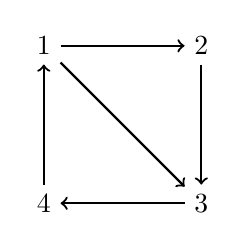
\begin{tikzpicture}
\node (atom1) at (0,2) {1};
\node (atom2) at (2,2) {2};
\node (atom3) at (2,0) {3};
\node (atom4) at (0,0) {4};
\draw[->, thick] (atom1)--(atom2);
\draw[->, thick] (atom2)--(atom3);
\draw[->, thick] (atom3)--(atom4);
\draw[->, thick] (atom4)--(atom1);
\draw[->, thick] (atom1) -- (atom3);
\end{tikzpicture}
\end{center}
Este diagrama é adequado para caracterizar uma interpretação cujo domínio são os números de $1$ a $4$ e que tem uma única relação binária `$\atom{R}{x,y}$', que é verdadeira dos seguintes pares:
	\begin{center}
		\ntuple{1, 2}, 
		\ntuple{2, 3}, 
		\ntuple{3, 4}, 
		\ntuple{4, 1}, 
		\ntuple{1, 3}
	\end{center}
Da mesma forma, podemos oferecer:

\begin{center}
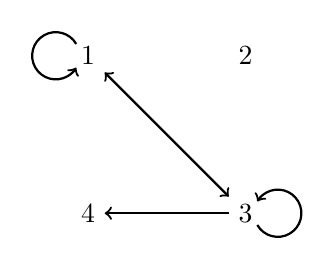
\begin{tikzpicture}
\node (atom1) at (0,2) {1};
\node (atom2) at (2,2) {2};
\node (atom3) at (2,0) {3};
\node (atom4) at (0,0) {4};
\draw[->, thick] (atom3)--(atom4);
\draw[->, thick] (atom1)+(-0.15,0.15) arc (-330:-30:.3); 
\draw[->, thick] (atom3)+(0.15,-0.15) arc (-150:150:.3); 
\draw[<->, thick] (atom1) -- (atom3);
\end{tikzpicture}
\end{center}
para uma interpretação com o mesmo domínio, e com uma relação binária `$\atom{R}{x,y}$' cuja extensão é dada pelos seguintes pares:
	\begin{center}
		\ntuple{1, 3}, 
		\ntuple{3, 1}, 
		\ntuple{3, 4}, 
		\ntuple{1, 1},
		\ntuple{3, 3}
	\end{center}
Se quisermos, podemos tornar nossos diagramas mais complexos. Por exemplo, podemos adicionar nomes como rótulos para objetos específicos.
Da mesma forma, para simbolizar a extensão de um predicado de um lugar, podemos simplesmente desenhar um anel em torno de alguns objetos específicos e estipular que os objetos assim circundados (e somente eles) satisfazem o predicado em questão. 


\chapter{A verdade na LPO}\label{s:TruthFOL}
Não custa nada relembrar aqui que o objetivo principal do estudo da lógica é avaliar argumentos, separando os válidos dos inválidos.
E também não custa nada relembrar que um argumento é válido quando suas premissas justificam sua conclusão, ou seja, quando não é possível haver uma situação em que suas premissas sejam todas verdadeiras, mas sua conclusão seja falsa.
Então, antes de sermos capazes de avaliar argumentos na LPO, precisamos ser capazes de ligar as sentenças da LPO a situações em que poderemos avaliar se elas são verdadeiras ou falsas.

%Na LVF, esta ponte entre as sentenças simbolizadas e as situações é feita pelas valorações.
Na LVF, esta ponte que nos possibilita interpretar sentenças simbolizadas em situações nas quais elas serão verdadeiras ou falsas é dada pelos esquemas de simbolização, juntamente com as valorações.
%Através de um esquema de simbolização, situações distintas produzem valorações distintas nas quais as sentenças são verdadeiras ou falsas;
Através de um esquema de simbolização, a verdade ou falsidade das sentenças em português nas diversas situações transforma-se na verdade ou falsidade das sentenças simbolizadas na LVF nas diversas valorações.
Um esquema de simbolização liga situações distintas a valorações distintas que correspondem às diversas linhas das tabelas de verdade, nas quais as sentenças da LPO são verdadeiras ou falsas.
E a consideração dos valores de verdade das sentenças em todas as valorações possíveis, feita nas tabelas de verdade, nos possibilita avaliar a validade dos argumentos.\footnote{
	Se quiser relembrar os detalhes deste processo na LVF, releia a Seção~\ref{s:SustentValid}, p.\,\pageref{s:SustentValid}.}
%e a consideração, através das tabelas de verdade, de todas as valorações possíveis, nos possibilita avaliar a validade dos argumentos.

No caso da LPO, esta ponte entre as sentenças simbolizadas e as situações é feita pela noção de interpretação, introduzida na Seção \ref{s:Interpret}, p.\,\pageref{s:Interpret}.
Vimos ali que uma interpretação é um esquema de simbolização composto por: 
\begin{ebullet}
	\item um domínio do discurso;
	\item uma atribuição (direta ou indireta) de valores de verdade para cada letra sentencial;
	\item a definição de uma referência, no domínio, para cada nome;
	\item a definição (dierta ou indireta) de uma extensão para cada predicado e relação.
\end{ebullet}
Um esquema de simbolização com todos esses componentes constitui uma interpretação e nos fornece tudo o que precisamos para decidir se uma sentença qualquer da LPO é verdadeira ou falsa.
Entender como utilizar interpretações para classificar as sentenças da LPO como verdadeiras ou falsas é o primeiro passo para conseguirmos avaliar argumentos na LPO, e será nossa tarefa neste capítulo.

Sabemos, do Capítulo \ref{s:FOLSentences}, que existem três tipos de sentenças na LPO:
	\begin{itemize}
		\item sentenças atômicas:
		\begin{ebullet}
			\item $\atom{C}{b}$
			\item $\atom{A}{r,j}$
			\item $Q$
		\end{ebullet}
		\item sentenças cujo operador principal é um conectivo sentencial:
		\begin{ebullet}
			\item $\atom{C}{b} \eand Q$
			\item $\atom{A}{r,j} \eif \forall x\,\atom{C}{x}$
			\item $\enot Q$
		\end{ebullet}
		\item sentenças cujo operador principal é um quantificador:
		\begin{ebullet}
			\item $\exists x\,\atom{C}{x}$
			\item $\forall x (\atom{A}{x,j} \eif \atom{C}{x})$
			\item $\exists x \exists y (\atom{A}{x,y} \eand \atom{A}{y,x})$
		\end{ebullet}
	\end{itemize}
Temos que explicar como atribuir valores de verdade para cada um destes tipos de sentenças.

A explicação que daremos aqui é completamente geral e vale para qualquer interpretação.
No entanto, para facilitar a compreensão, usaremos a seguinte interpretação como exemplo privilegiado:
\begin{center}\label{i:Sample}
	\begin{ekey}
		\item[\text{domínio}] {\footnotesize todas as pessoas (vivas ou mortas) nascidas antes do ano 2020}
		\item[a] {\small Aristóteles}
		\item[b] {\small Simona Talma}
		\item[C] {\small Simona Talma é uma artista potiguar\,}\footnote{
			Poderíamos aqui ter criado um predicado tal como `$\atom{P}{x}$' para `\gap{x}~é uma artista portiguar' e simbolizar `Simona Talma é uma artista potiguar' como `$\atom{P}{b}$'.
			Não fizemos isso porque queremos que a interpretação de nosso exemplo tenha também uma letra sentencial `$C$' que, tal  como na LVF, tem exatamente o mesmo valor de verdade que a sentença `Simona Talma é uma artista potiguar'.}
		\item[D] {\small é F (uma sentença falsa)}\footnote{
			Aqui estamos apenas indicando diretamente, sem nenhuma sentença em português intermediária, que a letra sentencial `$D$' é uma sentença falsa.}
		\item[\atom{F}{x}] \gap{x} {\small é filósofo}
		\item[\atom{R}{x,y}] \gap{x} {\small nasceu antes que} \gap{y}
	\end{ekey}
\end{center}
Esta interpretação será o nosso caso de estudo nas Seções seguintes.


\section{Sentenças atômicas}
Existem três tipos de sentenças atômicas na LPO, as letras sentenciais, tais como `$C$' e `$D$', os predicados seguidos de nomes, tais como  `$\atom{F}{a}$' e `$\atom{F}{b}$', e as relações $n$-árias seguidas de $n$-uplas ordenadas de nomes, tais como `$\atom{R}{a,b}$' e `$\atom{R}{b,a}$'.
Precisamos, então, entender como as interpretações atribuem valores de verdade para cada um desses três tipos de sentenças atômicas.

No caso das letras sentenciais, isso é uma operação imediata idêntica ao que fazíamos na LVF.
A interpretação estabelece direta ou indiretamente se a letra sentencial é verdadeira ou falsa.
Em nosso exemplo
\begin{center}
	$`C'$ \ \ é \ \ verdadeira   
\end{center}
porque Simona Talma é mesmo uma artista potiguar.
A interpretação nos dá aqui uma especificação indireta através da sentença em português `Simona Talma é uma artista potiguar'.
A letra sentencial terá o mesmo valor de verdade desta sentença.

Por outro lado,
\begin{center}
	$`D'$ \ \ é \ \ falsa   
\end{center}
porque a interpretação estabelece diretamente este fato, sem qualquer sentença intermediária.

%Se a sentença atômica for constituída por um predicado seguido de um nome, tal como `$\atom{F}{a}$', ela será verdadeira apenas no caso do predicado `$\atom{F}{x}$' ser verdadeiro do indivíduo que `$a$' nomeia.
Quando a sentença atômica é constituída por um predicado seguido de um nome, tal como `$\atom{F}{a}$', ela será verdadeira apenas no caso em que o indivíduo que `$a$' nomeia esteja na extensão do predicado `$\atom{F}{x}$'.
Em nossa interpretação, a extensão de `$\atom{F}{x}$' é dada indiretamente pelo predicado `\gap{x} é filósofo'.
Então,
\begin{center}
	`$\atom{F}{a}$' \ \ é \ \ verdadeira
\end{center}
já que `$a$' nomeia Aristóteles e Aristóteles é um filósofo.
De modo semelhante,
\begin{center}
	`$\atom{F}{b}$' \ \ é \ \ falsa
\end{center}
porque `$b$' nomeia Simona Talma, que não é uma filósofa.

Por fim, se a sentença atômica for uma relação seguida de uma sequência ordenada de nomes, tal como `$\atom{R}{a,b}$', ela será verdadeira apenas se o par ordenado dos indivíduos nomeados por `$a$' e `$b$', \ntuple{Aristóteles, Simona Talma}, estiver na extensão do predicado `$\atom{R}{x,y}$'.
Em nossa interpretação esta extensão é definida indiretamente através da relação
\begin{center}
	`\gap{x} nasceu antes que \gap{y}'.
\end{center}	
Como Aristóteles nasceu antes de Simona Talma, então o par \ntuple{Aristóteles, Simona Talma} está na extensão de `$\atom{R}{x,y}$' e
\begin{center}
	`$\atom{R}{a,b}$' \ \ é \ \ verdadeira
\end{center}
Da mesma forma, podemos facilmente verificar que 
\begin{center}
	`$\atom{R}{a,a}$' \ \ é \ \ falsa
\end{center}
porque Aristóteles não nasceu antes que Aristóteles.

Lidar com sentenças atômicas é, portanto, muito intuitivo.
As letras sentencias são tratadas exatamente do mesmo modo que na LVF e quando \meta{R} é um predicado $n$-lugares e \mbox{$\meta{a}_1 $, $\meta{a}_{2}$, \dots, $\meta{a}_{n}$} \ são nomes, temos:

	\factoidbox{
		$\atom{\meta{R}}{\meta{a}_{1},\meta{a}_{2},\dots,\meta{a}_{n}}$ é verdadeira em uma interpretação\\
		\textbf{se e somente se}\\
		$\meta{R}$ é verdadeira dos objetos nomeados por $\meta{a}_{1}$, $\meta{a}_{2}$, \dots, $\meta{a}_{n}$ na interpretação (considerados nesta ordem)
	}
Lembre-se, porém, de que existe um tipo especial de sentença atômica: dois nomes conectados por um sinal de identidade constituem uma sentença atômica.
Esse tipo de sentença atômica também é fácil de lidar.
Sejam \meta{a} e \meta{b} nomes quaisquer,
	\factoidbox{
		$\meta{a} = \meta{b}$ é verdadeira em uma interpretação\\
		\textbf{se e somente se}\\
		 \meta{a} e \meta{b} são nomes do mesmo objeto nesta interpretação
	}
Portanto, em nossa interpretação,
\begin{center}
	`$a=b$' \ \ é \ \ falsa
\end{center}
porque Aristóteles e Simona Talma não são a mesma pessoa.


\section{Conectivos sentenciais}
Vimos no Capítulo \ref{s:FOLSentences} que as sentenças da LPO podem ser criadas a partir de sentenças mais simples, usando os conectivos verofuncionais da LVF. As regras que governam a atribuição de verdade ou falsidade a sentenças deste tipo na LPO são \emph{exatamente} as mesmas da LVF.
Aqui estão elas:
	\factoidbox{
		$\meta{A} \eand \meta{B}$ é verdadeira em uma interpretação\\ \textbf{se e somente se}\\
		$\meta{A}$ e $\meta{B}$ são ambas verdadeiras nesta interpretação
		
		\bigskip
		$\meta{A} \eor \meta{B}$ é verdadeira em uma interpretação\\  \textbf{se e somente se}\\
		$\meta{A}$ é verdadeira ou $\meta{B}$ é verdadeira nesta interpretação

		\bigskip
		$\enot \meta{A}$ é verdadeira em uma interpretação\\ \textbf{se e somente se}\\
		$\meta{A}$ é falsa nesta interpretação

		\bigskip
		$\meta{A} \eif \meta{B}$ é verdadeira em uma interpretação\\ \textbf{se e somente se}\\
		$\meta{A}$ é falsa ou $\meta{B}$ é verdadeira nesta interpretação

		\bigskip
		$\meta{A} \eiff \meta{B}$ é verdadeira em uma interpretação\\ \textbf{se e somente se}\\
		$\meta{A}$ e $\meta{B}$ têm o mesmo valor de verdade nesta interpretação
	}\label{b:ConSent}
Estas definições nos dão, de um modo diferente, exatamente a mesma informação que as tabelas de verdade características dos conectivos, que vimos no Capítulo \ref{s:CharacteristicTruthTables}, p.\,\pageref{s:CharacteristicTruthTables}.
Alguns exemplos nos ajudarão aqui.
A ideia é aplicar as definições do quadro acima à nossa interpretação exemplo (p.\,\pageref{i:Sample}) para decidir o valor de verdade das sentenças:
	\begin{earg}
		\item[\textbullet] `$a = a \eand \atom{F}{a}$' \ \ é \ \ verdadeira\\
			porque tanto `$a = a$' quanto `$\atom{F}{a}$' são verdadeiras
		\item[\textbullet] `$\atom{R}{a,b} \eand \atom{F}{b}$' \ \ é \ \ falsa\\
			porque ainda que `$\atom{R}{a,b}$' seja verdadeira, `$\atom{F}{b}$' é falsa\\
		\item[\textbullet] `$a = b \eor \atom{F}{a}$' \ \ é \ \ verdadeira\\
			porque ainda que  `$a = b$' seja falsa, `$\atom{F}{a}$' é verdadeira\\
		\item[\textbullet] `$\enot a = b$' \ \ é \ \ verdadeira\\
			porque `$a = b$' é falsa\\
		\item[\textbullet] `$\atom{F}{a} \eand \enot( a= b \eand \atom{R}{a,b})$' \ \ é \ \ verdadeira\\
			porque `$\atom{F}{a}$' é verdadeira e `$a = b$' é falsa
	\end{earg}
Antes de prosseguir, certifique-se de ter compreendido todos esses exemplos.
Simplesmente aplicamos, em cada caso, a definição correspondente do quadro acima (p.\,\pageref{b:ConSent}). 


\section[Quantificadores]{Quando o operador principal é um quantificador}\label{s:MainLogicalOperatorQuantifier}
Até aqui viemos bem, mas ainda não tratamos do aspecto que representa a principal novidade introduzida na LPO:
as sentenças cujo operador principal é um \emph{quantificador}.
Veremos que expressar as condições de verdade deste tipo de sentenças é um pouco mais complicado do que parece à primeira vista.
A ideia geral até que é simples e já foi mencionada de passagem em capítulos anteriores:
	\begin{earg}
		\item[\textbullet] $\forall x \atom{\meta{A}}{x}$ é verdadeira \ \ \textbf{se e somente se}\\
		$\atom{\meta{A}}{x}$ for verdadeira \textit{de todos} os elementos do domínio.\\
		\item[\textbullet] $\exists x \atom{\meta{B}}{x}$ é verdadeira \ \ \textbf{se e somente se}\\
		$\atom{\meta{B}}{x}$ for verdadeira \textit{de algum} elemento do domínio.
	\end{earg}
A dificuldade maior não é esta ideia geral, mas a especificação de sua definição precisa.

Vamos aqui nos aproximar pouco a pouco da definição.
Começaremos com algumas propostas ingênuas e vamos corrigindo-as até, eventualmente, chegarmos à definição correta.
Uma primeira proposta é a seguinte:
se, como vimos, `$\forall x\,\atom{F}{x}$' deve ser verdadeira se e somente se `$\atom{F}{x}$' é verdadeira para tudo no domínio,
então poderíamos simplesmente considerar que uma sentença universal é verdadeira quando a extensão do predicado que a segue compreende todo o domínio do discurso.

Esta idéia funciona quando o que vem após o quantificador inicial é um predicado, como em  `$\forall x\,\atom{F}{x}$'.
Mas, infelizmente, essa ideia não é geral o suficiente para especificar as condições de verdade de sentenças onde o que segue o quantificador inicial não é um predicado, mas outra expressão quantificada, tal como ocorre em:
$$\forall x \exists y\,\atom{L}{x,y}$$
Não conseguimos aplicar esta ideia aqui, porque o que segue o quantificador não é um predicado, mas a expressão quantificada `$\exists y\,\atom{L}{x,y}$'.
E as interpretações não têm cláusulas que indicam se `$\exists y\,\atom{L}{x,y}$' é verdadeira de tudo no domínio.
As cláusulas das intepretações especificam apenas a referência de nomes e a extensão de predicados e relações.

Para tentar corrigir isso poderíamos então sugerir que `$\forall x \exists y\, \atom{L}{x,y}$' deve ser verdadeira em uma interpretação se e somente se $\exists y\, \atom{L}{\meta{a},y}$ for verdadeira para \emph{todo} nome \meta{a} da interpretação.
E, de modo similar, diríamos que $\exists y\, \atom{L}{\meta{a},y}$ é verdadeira se e somente se $\atom{L}{\meta{a}, \meta{b}}$ for verdadeira para \emph{algum} nome \meta{b}.
Então, juntando estes dois passos, `$\forall x \exists y\, \atom{L}{x,y}$' seria verdadeira em uma interpretação se e somente se $\atom{L}{\meta{a}, \meta{b}}$ for verdadeira para \emph{todo} nome \meta{a} e \emph{algum} nome \meta{b} presentes na interpretação.

Infelizmente, isso também não funciona.
Para entender por que, basta observar que na interpretação de nossos exemplos (p.\,\pageref{i:Sample}), apenas duas pessoas têm nome, mas o domínio comporta todas as pessoas nascidas antes do ano 2020.

Uma terceira ideia, então, é a seguinte.
Mesmo que uma interpretação não tenha nomes para \emph{todos} os indivíduos do domínio, ela poderia ter.
Ou seja, podemos estender uma interpretação qualquer, de modo a que todos os elementos do domínio tenham nomes.
Antes de prosseguir com a definição, vejamos alguns exemplos de como isso pode funcionar.

Em nossa interpretação privilegiada (p.\,\pageref{i:Sample}) `$\exists x\, \atom{R}{b,x}$' deve ser verdadeira. Afinal, certamente há no domínio alguém que nasceu depois que Simona Talma.
Dani Cruz (uma outra artista potiguar) é uma dessas pessoas.
De fato, se estendermos temporariamente nossa interpretação adicionando o nome `$c$' para se referir a Dani Cruz, então `$\atom{R}{b,c}$' será verdadeira nessa interpretação estendida.
E este fato certamente deve ser suficiente para assegurar que `$\exists x\,\atom{R}{b,x}$' é verdadeira na nossa interpretação original, já que ele indica que há pelo menos uma pessoa no domínio (Dani Cruz) que nasceu depois de Simona Talma.

Na nossa interpretação, `$\exists x (\atom{F}{x} \eand \atom{R}{x,a})$' também deve ser verdadeira.
Afinal, no domínio, certamente há alguém que foi filósofo e nasceu antes de Aristóteles.
Sócrates é uma dessas pessoas.
De fato, se estendermos nossa interpretação, com um novo nome, `$d$', que denota Sócrates, então `$\atom{F}{d} \eand \atom{R}{d,a}$' será verdadeira nessa interpretação estendida.
Novamente, isso certamente é suficiente como garantia de que `$\exists x (\atom{F}{x} \eand \atom{R}{x,a})$' é verdadeira na interpretação original (não estendida), já que isso indica que há pelo menos uma pessoa no domínio (Sócrates) que é filósofo e nasceu antes de Aristóteles.

Já a sentença `$\forall x \exists y\, \atom{R}{x,y}$' deve ser falsa em nossa interpretação.
Afinal, certamente há uma última pessoa que nasceu antes do ano 2020 começar.
Não sabemos quem é esta pessoa, mas podemos, mesmo assim, estender a interpretação para que um nome novo, `$e$', denote exatamente esta pessoa.
E fazendo isso, qualquer que seja o indivíduo do domínio ao qual um outro nome novo $`f'$ se refira, a sentença `$\atom{R}{e,f}$' seria falsa.
De fato, não importa \emph{quem} seja a referência do nome `$f$', sabemos que `$\atom{R}{e,f}$' será falsa, já que `$e$' denota a última pessoa nascida em 2019. 
Esse fato é certamente suficiente para garantir que `$\exists y\, \atom{R}{e,y}$' é falsa na interpretação estendida. E isso, por sua vez, é certamente suficiente como garantia de que `$\forall x \exists y\, \atom{R}{x,y}$' é falsa na nossa interpretação original.

Se você entendeu esses três exemplos, ótimo. É isso que importa.
O que temos que fazer, agora, é fornecer uma definição precisa dessas ideias, que exprima as condições de verdade para sentenças quantificadas.
Para isso precisamos de mais notação em nossa metalinguagem.
A expressão:
$$\meta{A}(\meta{x})$$
será usada para denotar na metalinguagem uma fórmula que contenha pelo menos uma ocorrência livre da variável \meta{x}.
Ou seja, há uma ou mais ocorrências de \meta{x} em \meta{A} que estão fora do escopo de qualquer `$\forall x$' e `$\exists x$' em \meta{A}.
Seja \meta{c} um nome.
A expressão:
$$\meta{A}(\meta{c})$$
será usada para denotar na metalinguagem a fórmula obtida quando substituímos por $\meta{c}$ \emph{todas} as ocorrências livres de $\meta{x}$ em \meta{A}.
A fórmula resultante, $\meta{A}(\meta{c})$, é chamada de \define{instancia de substituicao} de $\forall \meta{x} \meta{A}$ e $\exists \meta{x} \meta{A}$.
Além disso, $\meta{c}$ é chamado de \define{nome de instanciacao}.

Vejamos um exemplo.
Considere a sentença da LPO:
	$$\forall y \exists x (\atom{R}{y,x} \eiff \atom{F}{x})$$
A notação recém  introduzida nos permite usar a expressão
	$$\forall \meta{y} \atom{\meta{A}}{\meta{y}}$$
para nos referirmos a esta sentença de um modo genérico em nossa metalinguagem.
Quando fazemos isso, a expressão
	$$\atom{\meta{A}}{\meta{y}}$$
refere-se genericamente a
	$$\exists x (\atom{R}{y,x} \eiff \atom{F}{x})$$
que é uma fórmula com uma ocorrência livre da variável `$y$'.
Se substituímos esta ocorrência livre de `$y$' por um nome, digamos, `$e$', obtemos a sentença:
	$$\exists x (\atom{R}{e,x} \eiff \atom{F}{x})$$
Esta sentença nada mais é do que uma instância de substituição de 
	$$\forall y \exists x (\atom{R}{y,x} \eiff \atom{F}{x})$$
onde `$e$' é o nome de instanciação, e `$y$' é a variável instanciada.

\newglossaryentry{substitution instance}{
  name = substitution instance,
  description = {The result of replacing every free occurrence of a \gls{variable} in a \gls{formula} with a \gls{name}}
}

Seja $\mathbf{I}$ o nome de uma interpretação que estejamos considerando.
$\mathbf{I}$ inclui uma especificação de quais nomes correspondem a quais objetos no domínio.
Considere um objeto  qualquer do domínio, digamos, $d$, e um nome $\meta{c}$ que não esteja sendo usado em $\mathbf{I}$.
Usaremos a notação
$$\mathbf{I}[d/\meta{c}]$$
para nos referirmos à interpretação que é igual a $\mathbf{I}$, com um acréscimo:
$\mathbf{I}[d/\meta{c}]$ atribui o nome $\meta{c}$ ao objeto $d$.
Então podemos dizer que $d$ \define{satisfaz} a fórmula $\meta{A}(\meta{x})$ na interpretação $\mathbf{I}$ se e somente se $\meta{A}(\meta{c})$ é verdadeira em $\mathbf{I}[d/\meta{c}]$.
(Quando $d$ satisfaz $\meta{A}(\meta{x})$, nós dizemos também que $\meta{A}(\meta{x})$ é \emph{verdadeira de} $d$.

\factoidbox{A interpretação $\mathbf{I}[d/\meta{c}]$ é igual à interpretação $\mathbf{I}$, com o acréscimo de que atribui o nome $\meta{c}$ ao objeto $d$.

\
\\
Um objeto $d$ \define{satisfaz} $\meta{A}(\meta{x})$ na interpretação $\mathbf{I}$ \\
\hbox{\textbf{se e somente se}} $\meta{A}(\meta{c})$ é verdadeira em $\mathbf{I}[d/\meta{c}]$.
}

\noindent Assim, por exemplo, dizemos que: 
\begin{ebullet}
	\item Sócrates \underline{satisfaz} a fórmula `$\atom{F}{x}$'
\end{ebullet}
pois:
\begin{ebullet}
	\item $\atom{F}{c}$ é \underline{verdadeira} na interpretação $\mathbf{I}[\text{Sócrates}/c]$
\end{ebullet}
ou seja, $\atom{F}{c}$ é verdadeira na interpretação que obtemos de nossa interpretação original $\mathbf{I}$ (p.\pageref{i:Sample}) quando acrescentamos a indicação de que o nome `$c$' se refere a Sócrates:

\begin{center}
	\begin{ekey}
		\item[\text{domínio}] {\footnotesize todas as pessoas (vivas ou mortas) nascidas antes do ano 2020}
		\item[a] {\small Aristóteles}
		\item[b] {\small Simona Talma}
		\item[c] {\small Sócrates}
		\item[C] {\small Simona Talma é uma artista potiguar\,}
		\item[D] {\small é F (uma sentença falsa)}
		\item[\atom{F}{x}] \gap{x} {\small é filósofo}
		\item[\atom{R}{x,y}] \gap{x} {\small nasceu antes que} \gap{y}
	\end{ekey}
\end{center}

Tendo ampliado nossa metalinguagem com estas notações, podemos finalmente definir as condições de verdade de sentenças da LPO cujo operador principal é um quantificador.
A ideia aproximada é a seguinte.
A sentença $\forall \meta{x}\meta{A}(\meta{x})$ será verdadeira em $\mathbf{I}$ se e somente se, para qualquer objeto $d$ no domínio, $\meta{A}(\meta{c})$ é verdadeira em $\mathbf{I}[d/\meta{c}]$.
Ou seja, $\forall \meta{x}\meta{A}(\meta{x})$ será verdadeira  se e somente se $\meta{A}(\meta{c})$ for verdadeira, independentemente de qual objeto (no domínio) tenha sido nomeado  por $\meta{c}$.
Em outras palavras, $\forall \meta{x} \meta{A}(\meta{x})$ é verdadeira apenas quando todos os objetos no domínio satisfazem $\meta{A}(\meta{x})$.

Similarmente, a sentença $\exists \meta{x}\meta{A}(\meta{x})$ será verdadeira se e somente se houver \emph{algum} objeto no domínio que satisfaça $\meta{A}(\meta{x})$.
Ou seja, $\exists \meta{x}\meta{A}(\meta{x})$ é verdadeira em $\mathbf{I}$ se e somente se  $\meta{A}(\meta{c})$ é verdadeira em $\mathbf{I}[d/\meta{c}]$ para pelo menos um objeto $d$.
	\factoidbox{
		$\forall \meta{x}\meta{A}(\meta{x})$ é \underline{verdadeira} em uma interpretação \textbf{se e somente se} todo objeto no domínio \underline{satisfiaz} $\meta{A}(\meta{x})$.
		
		\
		\\
		$\exists \meta{x}\meta{A}(\meta{x})$ é \underline{verdadeira} em uma interpretação \textbf{se e somente se} pelo menos um objeto no domínio \underline{satisfaz} $\meta{A}(\meta{x})$.
	}
Para ficar claro: tudo o que estamos fazendo aqui é formalizar (de um modo bastante preciso) a ideia intuitiva de que para que uma sentença quantifidada universalmente seja verdadeira, todos os objetos do domínio precisam satisfazê-la; e para que uma sentença quantificada existencialmente seja verdadeira, basta que um objeto do domínio a satisfaça. 

Finalmente, vale notar que o conceito de um objeto satisfazer uma fórmula com uma variável livre também pode ser estendido a fórmulas com mais de uma variável livre.
Por exemplo, se tivermos uma fórmula $\meta{A}(\meta{x},\meta{y})$ com duas variáveis livres $\meta{x}$ e $\meta{y}$, podemos dizer que um par de objetos $\langle a, b\rangle$ satisfaz $\meta{A}(\meta{x},\meta{y})$ se e somente se $\meta{A}(\meta{c},\meta{d})$ for verdadeira na interpretação estendida por dois nomes $\meta{c}$ e $\meta{d}$, onde $\meta{c}$ é o nome de $a$ e $\meta{d}$ é o nome de $b$.
Assim, por exemplo, $\langle \text{Sócrates}, \text{Platão}\rangle$ satisfaz $R(x,y)$, pois, já que Sócrates nasceu antes de Platão, $R(c,d)$ é verdadeiro na interpretação:
\begin{center}
	\begin{ekey}
		\item[\text{domínio}] {\footnotesize todas as pessoas (vivas ou mortas) nascidas antes do ano 2020}
		\item[a] {\small Aristóteles}
		\item[b] {\small Simona Talma}
		\item[c] {\small Sócrates}
		\item[d] {\small Platão}
		\item[C] {\small Simona Talma é uma artista potiguar\,}
		\item[D] {\small é F (uma sentença falsa)}
		\item[\atom{F}{x}] \gap{x} {\small é filósofo}
		\item[\atom{R}{x,y}] \gap{x} {\small nasceu antes que} \gap{y}
	\end{ekey}
\end{center}
Para fórmulas atômicas, tais como $\atom{F}{x}$ e $\atom{R}{x,y}$,  os objetos ou sequências de objetos que as satisfazem são exatamente a extensão dos predicados que as constituem.
Mas a noção de satisfação também se aplica a fórmulas não atômicas.
A fórmula $\atom{F}{x} \land \atom{R}{x,b}$, por exemplo, é satisfeita por todos os filósofos que nasceram antes de Simona Talma.
A ideia de satisfação aplica-se até mesmo a fórmulas envolvendo quantificadores.
Por exemplo, $F(x) \eand \lnot\exists y(F(y) \land R(y,x))$ é satisfeita por todos os filósofos para os quais nenhum filósofo nasceu antes deles---em outras palavras, o primeiro filósofo, e apenas ele, satisfaz esta fórmula.


\practiceproblems
\solutions
\problempart
\label{pr.TorF1}
Considere a seguinte interpretação:
	\begin{ebullet}\small
		\item O domínio compreende apenas Benedita e Clayton
		\item `$\atom{A}{x}$' é verdadeira para ambos, tanto Benedita quanto Clayton
		\item `$\atom{B}{x}$' é verdadeira apenas para Benedita
		\item `$\atom{N}{x}$' não é verdadeira nem para Benedita nem para Clayton
		\item `$c$' refere-se a Clayton
	\end{ebullet}
Para cada uma das nove sentenças seguintes, determine se ela é verdadeira ou falsa nesta interpretação.
\begin{earg}
\item $\atom{B}{c} $
\item $\atom{A}{c}  \eiff \enot \atom{N}{c}$
\item $\atom{N}{c}  \eif (\atom{A}{c} \eor \atom{B}{c})$
\item $\forall x\, \atom{A}{x}$
\item $\forall x \enot \atom{B}{x}$
\item $\exists x(\atom{A}{x} \eand \atom{B}{x})$
\item $\exists x(\atom{A}{x} \eif \atom{N}{x})$
\item $\forall x(\atom{N}{x} \eor \enot \atom{N}{x})$
\item $\exists x\, \atom{B}{x} \eif \forall x\, \atom{A}{x}$
\end{earg}

\problempart
\label{pr.TorF2}
Considere a seguinte interpretação:	
	\begin{ebullet}
		\item O domínio compreende apenas Leila, Cora e Ênio
		\item `$\atom{G}{x}$' é verdadeira de Leila, de Cora e de Ênio
		\item `$\atom{H}{x}$' é verdadeira apenas de Cora
		\item `$\atom{M}{x}$' é verdadeira apenas de Leila e Ênio
		\item `$c$' refere-se a Cora
		\item `$e$' refere-se a Ênio
	\end{ebullet}
Para cada uma das quinze sentenças seguintes, determine se ela é verdadeira ou falsa nesta interpretação.
\begin{earg}
\item $\atom{H}{c} $
\item $\atom{H}{e} $
\item $\atom{M}{c}  \eor \atom{M}{e}$
\item $\atom{G}{c}  \eor \enot \atom{G}{c}$
\item $\atom{M}{c}  \eif \atom{G}{c}$
\item $\exists x\, \atom{H}{x}$
\item $\forall x\, \atom{H}{x}$
\item $\exists x\, \enot \atom{M}{x}$
\item $\exists x(\atom{H}{x} \eand \atom{G}{x})$
\item $\exists x(\atom{M}{x} \eand \atom{G}{x})$
\item $\forall x(\atom{H}{x} \eor \atom{M}{x})$
\item $\exists x\, \atom{H}{x} \eand \exists x\, \atom{M}{x}$
\item $\forall x(\atom{H}{x} \eiff \enot \atom{M}{x})$
\item $\exists x\, \atom{G}{x} \eand \exists x \enot \atom{G}{x}$
\item $\forall x\exists y(\atom{G}{x} \eand \atom{H}{y})$
\end{earg}

\problempart
\label{pr.TorF3}
Conforme as convenções introduzidas no final do Capítulo~\ref{s:Interpretations} (p.\,\pageref{s:Interpret}), o diagrama abaixo especifica uma interpretação cujo domínio é o conjunto $\{1,2,3,4,5\}$ e que tem uma única relação binária $\atom{R}{x,y}$, cuja extensão é dada pelas setas do diagrama:
\begin{center}
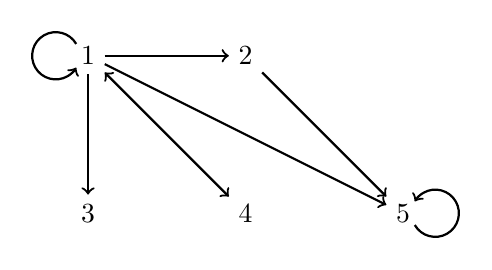
\begin{tikzpicture}
\node (atom1) at (0,2) {1};
\node (atom2) at (2,2) {2};
\node (atom4) at (0,0) {3};
\node (atom5) at (2,0) {4};
\node (atom6) at (4,0) {5};
\draw[->, thick] (atom1)+(-0.15,0.15) arc (-330:-30:.3); 
\draw[->, thick] (atom6)+(0.15,-0.15) arc (-150:150:.3); 
\draw[->, thick] (atom1) -- (atom2);
\draw[->, thick] (atom1) -- (atom4);
\draw[<->, thick] (atom1) -- (atom5);
\draw[->, thick] (atom1) -- (atom6);
\draw[->, thick] (atom2) -- (atom6);
\end{tikzpicture}
\end{center}
Para cada uma das doze sentenças seguintes, determine se ela é verdadeira ou falsa nesta interpretação.
\begin{earg}
\item $\exists x\, \atom{R}{x,x}$
\item $\forall x\, \atom{R}{x,x}$
\item $\exists x \forall y\, \atom{R}{x,y}$
\item $\exists x \forall y\, \atom{R}{y,x}$
\item $\forall x \forall y \forall z ((\atom{R}{x,y} \eand \atom{R}{y,z}) \eif \atom{R}{x,z})$
\item $\forall x \forall y \forall z ((\atom{R}{x,y} \eand \atom{R}{x,z}) \eif \atom{R}{y,z})$
\item $\exists x \forall y\, \enot \atom{R}{x,y}$
\item $\forall x(\exists y\, \atom{R}{x,y} \eif \exists y\, \atom{R}{y,x})$
\item $\exists x \exists y (\enot x = y \eand \atom{R}{x,y} \eand \atom{R}{y,x})$
\item $\exists x \forall y(\atom{R}{x,y} \eiff x = y)$
\item $\exists x \forall y(\atom{R}{y,x} \eiff x = y)$
\item $\exists x \exists y(\enot x = y \eand \atom{R}{x,y} \eand \forall z(\atom{R}{z,x} \eiff y = z))$
\end{earg}


\chapter{Conceitos semânticos}

Oferecer uma definição precisa de sentença verdadeira na LPO foi um pouco complicado, mas agora que terminamos, podemos definir várias noções lógicas importantes.
Elas serão muito parecidas com as definições que oferecemos para a LVF.
No entanto, lembre-se de que agora elas se referem a \emph{interpretações}, e não mais a valorações.

Continuaremos a usar o símbolo `$\entails$' na LPO da mesma forma que o utilizamos na LVF.
Assim:
	$$\meta{A}_1, \meta{A}_2, \ldots, \meta{A}_n \entails\meta{C}$$
significa que não há interpretação na qual $\meta{A}_1$, $\meta{A}_2$, \dots, $\meta{A}_n$ sejam todas verdadeiras e \meta{C} seja falsa. Consequentemente,
	$$\entails\meta{A}$$
significa que \meta{A} é verdadeira em todas as interpretações, ou seja, que é impossível que \meta{A} seja falsa.

As outras noções lógicas que vimos, também têm definições correspondentes na LPO.
Aqui estão elas:

\begin{itemize}
\item Uma sentença  $\meta{A}$ é uma \define{validade} na LPO se e somente se $\meta{A}$ for verdadeira em todas as interpretações; ou seja, se
$$\entails\meta{A}$$
\newglossaryentry{validity}
{
name=validity,
description={A \gls{sentence of FOL} that is true in every \gls{interpretation}}
}
\item $\meta{A}$ é uma \define{contradicao} na LPO se e somente se $\meta{A}$ for falsa em todas as interpretações; ou seja, se
$$\entails\enot\meta{A}$$
\newglossaryentry{contradiction of FOL}
{
  name=contradiction (of FOL),
  text=contradiction,
description={A \gls{sentence of FOL} that is false in every \gls{interpretation}}
}  
\item $\meta{A}_1, \meta{A}_2, \ldots \meta{A}_n \therefore \meta{C}$ é um argumento \define{valido na LPO} se e somente se não houver interpretação em que todas as premissas são verdadeiras e a conclusão é falsa; ou seja, se
$$\meta{A}_1,\meta{A}_2,\ldots \meta{A}_n \entails\meta{C}$$

\item Um argumento $\meta{A}_1, \meta{A}_2, \ldots \meta{A}_n \therefore \meta{C}$ é \define{invalido na LPO} se e somente se ele não é válido, ou seja, quando há alguma interpretação na qual todas as suas premissas são verdadeiras e a conclusão é falsa.
Denotamos isso por:
$$\meta{A}_1,\meta{A}_2,\ldots \meta{A}_n \nvDash\meta{C}$$
 
\newglossaryentry{valid in FOL}
{
  name=validity of arguments (in FOL),
  text = valid,
description={A property held by arguments; an argument is valid if and only if no \gls{interpretation} makes all premises true and the conclusion false}
}

\item Duas sentenças da LPO \meta{A} e \meta{B} são \define{equivalentes} se e somente se em toda interpretação na qual uma é verdadeira, a outra também é; ou seja, se
\begin{center}
	$\meta{A}\entails\meta{B}$ \ \ \ e \ \ \ $\meta{B}\entails\meta{A}$
\end{center}

\newglossaryentry{equivalent in FOL}
{
  name=equivalence (in FOL),
  text = equivalent,
description={A property held by pairs of \glspl{sentence of FOL} if and only if the sentences have the same truth value in every \gls{interpretation}}
}

\item As sentenças $\meta{A}_1$, $\meta{A}_2$, \dots, $\meta{A}_n$ são \define{conjuntamente satisfatorias} na LPO se e somente se há alguma interpretação na qual todas são verdadeiras.
Eles são \define{conjuntamente insatisfatorias} se não houver tal interpretação.
\newglossaryentry{satisfiable in FOL}
{
  name=satisfiability (in FOL),
  text=jointly satisfiable,
description={A property held by \glspl{sentence of FOL} if and only if some \gls{interpretation} makes all the sentences true}
}
\end{itemize}


\chapter{Utilizando as interpretações}
\label{sec.UsingModels}

\section{Validades e contradições}
Suponha que queremos mostrar que
$$\exists x\, \atom{A}{x,x} \eif \atom{B}{d}$$
\emph{não é} uma validade.
Conforme a definição vista no capítulo anterior, temos que mostrar que esta  sentença não é verdadeira em todas as interpretações; isto é, que ela é falsa em alguma interpretação.
Então será suficiente fornecermos uma única interpretação na qual a sentença seja falsa.

Para que `$\exists x\,\atom{A}{x,x} \eif \atom{B}{d}$' seja falsa, o antecedente do condicional (`$\exists x\, \atom{A}{x,x}$') deve ser verdadeiro, e o consequente (`$\atom{B}{d}$') deve ser falso.
Para construir uma interpretação na qual isso ocorra, começamos especificando um domínio.
Manter o domínio pequeno facilita a especificação da extensão dos predicados; portanto, começaremos com um domínio com apenas um indivíduo.
Digamos, então, que o único indivíduo de nosso domínio seja a cidade de Fortaleza.
\begin{center}
	\begin{ekey}
		\item[\text{domínio}] Fortaleza
	\end{ekey}
\end{center}
Nossa sentença tem um nome, `$d$', que precisa nomear algo no domínio.
Então nossa única opção é definir que:
\begin{center}
	\begin{ekey}
		\item[d] Fortaleza
	\end{ekey}
\end{center}
Lembre-se de que queremos que `$\exists x\, \atom{A}{x,x}$' seja verdadeira; portanto, queremos que algum indivíduo do domínio relacione-se consigo mesmo através de `$A$'.
Podemos então propor a seguinte extensão para a relação `$A$':
\begin{center}
	\begin{ekey}
		\item[\atom{A}{x,y}] \gap{x} está no mesmo país que \gap{y}
	\end{ekey}
\end{center}
Agora, `$\atom{A}{d,d}$' é claramente verdadeira, portanto, `$\exists x\, \atom{A}{x,x}$' também é. 
Mas nós também queremos que `$\atom{B}{d}$' seja falsa; portanto, o indivíduo nomeado por `$d$' não deve estar na extensão de `$B$'.
Podemos simplesmente propor que:
\begin{center}
	\begin{ekey}
		\item[\atom{B}{x}] \gap{x} é a capital do Rio Grande do Norte
	\end{ekey}
\end{center}
Construímos uma interpretação em que `$\exists x\, \atom{A}{x,x}$' é verdadeira, mas `$\atom{B}{d}$' é falsa.
Logo, nesta interpretação `$\exists x\, \atom{A}{x,x} \eif \atom{B}{d}$' é falsa e portanto não é uma validade.

Com a mesma facilidade podemos mostrar que `$\exists x\atom{A}{x,x} \eif \atom{B}{d}$' não é uma contradição.
Precisamos apenas especificar uma interpretação na qual `$\exists x\atom{A}{x,x} \eif \atom{B}{d}$' seja verdadeira; ou seja, uma interpretação na qual `$\exists x\, \atom{A}{x,x}$' é falsa ou `$\atom{B}{d}$' é verdadeira.
Aqui está uma:
\begin{center}
	\begin{ekey}
		\item[\text{domínio}] Fortaleza
		\item[d] Fortaleza
		\item[\atom{A}{x,y}] \gap{x} está no mesmo país que \gap{y}
		\item[\atom{B}{x}] \gap{x} é a capital do Ceará
	\end{ekey}
\end{center}
Isso mostra que existe uma interpretação na qual `$\exists x\atom{A}{x,x} \eif \atom{B}{d}$' é verdadeira, e portanto, não é uma contradição.
	\factoidbox{
		Para mostrar que $\meta{A}$ \textbf{não é uma validade}, basta apresentar uma interpretação em que $\meta{A}$ seja falsa.\\
		
		Para mostrar que $\meta{A}$ \textbf{não é uma contradição}, basta apresentar uma interpretação em que $\meta{A}$ seja verdadeira.
	}


\section{Equivalência lógica}
Suponha que queiramos mostrar que
\begin{center}
	$\forall x\, \atom{S}{x}$ \ \ e \ \ $\exists x\, \atom{S}{x}$
\end{center}
\emph{não são} logicamente equivalentes.
Precisamos construir uma interpretação na qual as duas sentenças tenham valores de verdade diferentes.
Queremos que uma das sentenças seja verdadeira e o outra falsa.
Começamos especificando um domínio e, novamente, o menor possível, para facilitar as coisas.
Vamos, no entanto, precisar de pelo menos dois objetos.
(Se o domínio tiver um único objeto as sentenças terão o mesmo valor de verdade. 
Para perceber por que, proponha algumas interpretações com domínios de um único indivíduo e veja o que ocorre com o valor de verdade das duas sentenças.)
Considere, então, o seguinte domínio:
	\begin{center}
	\begin{ekey}
		\item[\text{domínio}] Jackson do Pandeiro, Luiz Gonzaga
	\end{ekey}
	\end{center}
Podemos fazer `$\exists x\, \atom{S}{x}$' ser verdadeira incluindo um dos indivíduos do domínio na extensão de `$S$', e podemos fazer `$\forall x\, \atom{S}{x}$' ser falsa, deixando um dos indivíduos do domínio fora da extensão de `$S$'.
Considere então:
	\begin{center}
	\begin{ekey}
		\item[\atom{S}{x}] \gap{x} toca pandeiro
	\end{ekey}
	\end{center}
Agora `$\exists x\, \atom{S}{x}$' é verdadeira, porque Jackson do Pandeiro satisfaz `$\atom{S}{x}$'.
De modo mais preciso, se estendermos nossa interpretação fazendo `$c$' nomear Jackson do Pandeiro, `$\atom{S}{c}$' torna-se uma sentença verdadeira nessa interpretação estendida.
Portanto, `$\exists x\, \atom{S}{x}$' é verdadeira na interpretação original.
Da mesma forma, `$\forall x\, \atom{S}{x}$' é falsa, porque Luiz Gonzaga não satisfaz `$\atom{S}{x}$'.
Mais precisamente, estender a interpretação fazendo o nome `$d$' se referir a Luiz Gonzaga, torna a sentença `$\atom{S}{d}$' falsa nessa interpretação estendida, já que Luiz Gonzaga não toca pandeiro.
Portanto, `$\forall x\, \atom{S}{x}$' é falso na interpretação original.
Então a interpretação original que propusemos
	\begin{center}
	\begin{ekey}
		\item[\text{domínio}] Jackson do Pandeiro, Luiz Gonzaga
		\item[\atom{S}{x}] \gap{x} toca pandeiro
	\end{ekey}
	\end{center}
comprova que `$\exists x\, \atom{S}{x}$' e `$\forall x\, \atom{S}{x}$' não são logicamente equivalentes, já que a primeira sentença é verdadeira e a segunda é falsa nessa interpretação.
	\factoidbox{
		Para mostrar que $\meta{A}$ e $\meta{B}$ não são logicamente equivalentes, basta encontrar uma interpretação em que uma sentença é verdadeira e a outra é falsa.
	}


\section{Validade, sustentação e satisfação}
Para testar a validade, a sustentação ou a satisfação, normalmente precisamos produzir interpretações capazes de determinam o valor de verdade de várias sentenças.
Considere o seguinte argumento na LPO:
\begin{earg}
	\item[] $\exists x(\atom{G}{x} \eif \atom{G}{a})$
	\item[\therefore ] $\exists x\, \atom{G}{x} \eif \atom{G}{a}$
\end{earg}
%$$\exists x(\atom{G}{x} \eif \atom{G}{a}) \therefore \exists x\, \atom{G}{x} \eif \atom{G}{a}$$
Para mostrar que este argumento é inválido, precisamos encontrar uma interpretação na qual a premissa seja verdadeira, mas a conclusão seja falsa.
A conclusão é um condicional; portanto, ela será falsa quando seu antecedente for verdadeiro e o consequente falso.
Claramente, nosso domínio deve conter dois objetos, um que esteja na extensão de `$G$' e um que não esteja.
Vamos tentar:
	\begin{center}
	\begin{ekey}
		\item[\text{domínio}] Karl Marx, Pelé
		\item[\atom{G}{x}] \gap{x} é co-autor de `O Manifesto Comunista'
		\item[a] Pelé
	\end{ekey}
	\end{center}
Nesta interpretação a sentença `$\atom{G}{a}$' é claramente falsa.
Afinal, Pelé foi o maior jogador de futebol que já houve, e não escreveu nenhum manifesto.
Já Karl Marx é reconhecidamente um dos autores de `O Manifesto Comunista', juntamente com  Friedrich Engels.
Então, `$\exists x\, \atom{G}{x}$' é verdadeira nessa interpretação.
Portanto, como `$\exists x\, \atom{G}{x}$' é verdadeira e `$\atom{G}{a}$' é falsa, a conclusão de nosso argumento, `$\exists x\, \atom{G}{x} \eif \atom{G}{a}$' é uma sentença falsa, conforme requerido.

Será que a premissa é verdadeira?
Sim!
Observe que `$\atom{G}{a} \eif \atom{G}{a}$' é verdadeira. (De fato, `$\atom{G}{a} \eif \atom{G}{a}$' é uma validade, verdadeira em qualquer interpretação)
Então, certamente `$\exists x (\atom{G}{x} \eif \atom{G}{a})$' é verdadeira.
Temos, portanto, uma interpretação na qual a premissa do argumento é verdadeira e a conclusão é falsa.
Logo o argumento é inválido. 

Observe que nossa interpretação mostra também que
\begin{center}
	`$\exists x(\atom{G}{x} \eif \atom{G}{a})$' \ \ \emph{não} sustenta \ \ `$\exists x\, \atom{G}{x} \eif \atom{G}{a}$'
\end{center}
já que nela a primeira sentenças é verdadeira e a segunda é falsa.
Nossa interpretação também mostra que as sentenças abaixo são conjuntamente satisfatórias, já ambas são verdadeiras nela
\begin{center}
	$\exists x (\atom{G}{x} \eif \atom{G}{a})$ \ \ e \ \ $\enot (\exists x\, \atom{G}{x} \eif \atom{G}{a})$
\end{center}

Vejamos mais um exemplo.
Considere:
\begin{earg}
	\item[] $\forall x \exists y\, \atom{L}{x,y}$
	\item[\therefore ] $\exists y \forall x\, \atom{L}{x,y}$
\end{earg}
%$$\forall x \exists y\, \atom{L}{x,y} \therefore \exists y \forall x\, \atom{L}{x,y}$$

Novamente, queremos mostrar que este argumento é inválido.
E fazemos isso propondo uma interpretação onde a premissa é verdadeira, mas a conclusão é falsa.
Aqui está uma sugestão:
	\begin{center}
	\begin{ekey}
		\item[\text{domínio}] todas as pessoas casadas
		\item[\atom{L}{x,y}] \gap{x} é casado(a) com \gap{y}
	\end{ekey}
	\end{center}
A premissa é claramente verdadeira nessa interpretação. Qualquer pessoa no domínio é casada com alguma pessoa, que, por ser casada, também está no domínio.
Logo, `$\forall x \exists y\, \atom{L}{x,y}$' é verdadeira.
Por outro lado, a conclusão, `$\exists y \forall x\, \atom{L}{x,y}$',  é claramente falsa, pois sua verdade exigiria que houvesse uma única pessoa que fosse casada com todas as outras pessoas no domínio, inclusive com ela mesma.
Portanto, o argumento tem premissa verdadeira e conclusão falsa nesta interpretação e, por isso, é inválido.

Como no exemplo anterior, podemos observar ainda, como consequência imediata, que as sentenças `$\forall x \exists y\, \atom{L}{x,y}$' e `$\enot\exists y \forall x\, \atom{L}{x,y}$' são conjuntamente satisfatórias e que `$\forall x \exists y\, \atom{L}{x,y}$' não sustenta `$\exists y \forall x\, \atom{L}{x,y}$'.

Para o nosso terceiro exemplo, vamos misturar as coisas um pouco.
Na Seção \ref{s:Interpret}, p.\,\pageref{s:Interpret}, descrevemos como apresentar algumas interpretações usando diagramas. Por exemplo:
\begin{center}
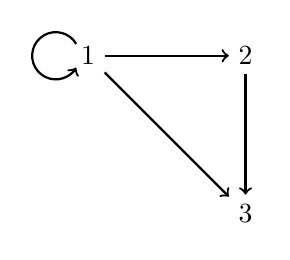
\begin{tikzpicture}
\node (atom1) at (0,2) {1};
\node (atom2) at (2,2) {2};
\node (atom3) at (2,0) {3};
\draw[->, thick] (atom1)--(atom2);
\draw[->, thick] (atom1)--(atom3);
\draw[->, thick] (atom1)+(-0.15,0.15) arc (-330:-30:.3); 
\draw[->, thick] (atom2) -- (atom3);
\end{tikzpicture}
\end{center}
De acordo com as convenções ali apresentadas, o domínio dessa interpretação são os três primeiros números inteiros positivos, e a extensão de  `$\atom{R}{x,y}$' é dada pelas setas do diagrama.
Ou seja, `$\atom{R}{x,y}$' é verdadeira para $\langle x, y \rangle$ apenas caso haja uma seta partindo  de \textbf{x} e chegando em \textbf{y} em nosso diagrama.
Aqui estão algumas sentenças verdadeiras nesta interpretação:
	\begin{ebullet}
		\item `$\forall x \exists y\, \atom{R}{y,x}$' 
		\item `$\exists x \forall y\, \atom{R}{x,y}$' \hfill  {\footnotesize 1 é uma testemunha}
		\item `$\exists x \forall y (\atom{R}{y,x} \eiff x = y)$' \hfill {\footnotesize 1 é uma testemunha}
		\item `$\exists x \exists y \exists z ((\enot y = z \eand \atom{R}{x,y}) \eand \atom{R}{z,x})$' \hfill {\footnotesize 2 é uma testemunha}
		\item `$\exists x \forall y\, \enot \atom{R}{x,y}$' \hfill {\footnotesize 3 é uma testemunha}
		\item `$\exists x (\exists y\, \atom{R}{y,x} \eand \enot \exists y\, \atom{R}{x,y})$' \hfill {\footnotesize 3 é uma testemunha}
	\end{ebullet}
Examíne-as com cuidado e certifieque-se de entender por que elas são todas verdadeiras na interpretação descrita pelo diagrama acima.\footnote{
	À direita de cada sentença existencial está indicada uma \textit{testemunha}, um elemento do domínio que satisfaz a fórmula existêncialmente quantificada.
	Ou seja, cada uma destas sentenças é do tipo $\exists x \atom{\meta{A}}{x}$ e cada testemunha indicada corresponde a um indivíduo $\meta{c}$ do domínio para o qual $\atom{\meta{A}}{\meta{c}}$ é verdadeira na interpretação.}	
	
Isso também mostra que essas seis sentenças são conjuntamente satisfatórias.
Podemos, então, usar esta observação para gerar argumentos \emph{inválidos}, tais como:
\begin{earg}
	\item[] $\forall x \exists y\, \atom{R}{y,x}$
	\item[] $\exists x \forall y\, \atom{R}{x,y}$
	\item[\therefore] $\forall x \exists y\, \atom{R}{x,y}$\footnote{
		Esta sentença não está entre os exemplos acima, porque ela é falsa em nossa interpretação.
		Para perceber isso basta notar que o indivíduo 3 é uma \textit{contratestemunha}, ou seja, é um elemento do domínio que não satisfaz a fórmula quantificada universalmente.}
\end{earg}
e
\begin{earg}
	\item[] $\exists x \forall y\, \atom{R}{x,y}$
	\item[] $\exists x \forall y \enot \atom{R}{x,y}$
	\item[\therefore] $\enot \exists x \exists y \exists z (\enot y = z \eand (\atom{R}{x,y} \eand \atom{R}{z,x}))$
\end{earg}

	\factoidbox{
	Ao apresentar uma interpretação em que  $\meta{A}_1$, $\meta{A}_2$, \dots, $\meta{A}_n$ são todas verdadeiras e onde $\meta{C}$ é falsa, nós mostramos que:
	\begin{ebullet}
		\item o argumento $\meta{A}_1, \meta{A}_2, \ldots, \meta{A}_n \therefore \meta{C}$ é inválido.
		\item $\meta{A}_1$, $\meta{A}_2$, \dots, $\meta{A}_n$ não sustentam $\meta{C}$.
		\item $\meta{A}_1$, $\meta{A}_2$, \dots, $\meta{A}_n$, $\enot \meta{C}$ são conjuntamente satisfatórias.
	\end{ebullet}}
Uma interpretação que refuta uma proposta, ou seja, que mostra que um argumento \emph{não} é válido, ou que uma sentença \emph{não} é uma validade (logicamente necessária), ou que um conjunto de sentenças \emph{não} sustenta uma outra sentença, é chamada de \emph{contrainterpretação} ou \emph{contramodelo}.



\practiceproblems

\solutions
\problempart
\label{pr.Contingent}
Mostre que cada uma das seguintes sete sentenças não é nem uma validade (necessidade lógica) nem uma contradição.
\begin{earg}
\item \leftsolutions\ $\atom{D}{a}  \eand \atom{D}{b}$
\item \leftsolutions\ $\exists x\, \atom{T}{x,h}$
\item \leftsolutions\ $\atom{P}{m}  \eand \enot\forall x\, \atom{P}{x}$
\item $\forall z \atom{J}{z} \eiff \exists y\, \atom{J}{y}$
\item $\forall x (\atom{W}{x,m,n} \eor \exists y\atom{L}{x,y})$
\item $\exists x (\atom{G}{x} \eif \forall y\, \atom{M}{y})$
\item $\exists x (x = h \eand x = i)$
\end{earg}

\solutions
\problempart
\label{pr.NotEquiv}
Mostre que as sentenças de cada um dos nove pares seguintes não são logicamente equivalentes.
\begin{earg}
\item $\atom{J}{a} $,  $\atom{K}{a}$
\item $\exists x\, \atom{J}{x}$,  $\atom{J}{m}$
\item $\forall x\, \atom{R}{x,x}$, $\exists x\, \atom{R}{x,x}$
\item $\exists x\, \atom{P}{x} \eif \atom{Q}{c}$, $\exists x (\atom{P}{x} \eif \atom{Q}{c})$
\item $\forall x(\atom{P}{x} \eif \enot \atom{Q}{x})$, $\exists x(\atom{P}{x} \eand \enot \atom{Q}{x})$
\item $\exists x(\atom{P}{x} \eand \atom{Q}{x})$, $\exists x(\atom{P}{x} \eif \atom{Q}{x})$
\item $\forall x(\atom{P}{x}\eif \atom{Q}{x})$, $\forall x(\atom{P}{x} \eand \atom{Q}{x})$
\item $\forall x\exists y\, \atom{R}{x,y}$, $\exists x\forall y\, \atom{R}{x,y}$
\item $\forall x\exists y\, \atom{R}{x,y}$, $\forall x\exists y\, \atom{R}{y,x}$
\end{earg}

\problempart
Mostre que as sentenças de cada um dos treze grupos abaixo são conjuntamente satisfatórias.
\begin{earg}
\item  $\atom{M}{a}, \enot \atom{N}{a}, \atom{P}{a}, \enot \atom{Q}{a}$
\item $\atom{L}{e,e}, \atom{L}{e,g}, \enot \atom{L}{g,e}, \enot \atom{L}{g,g}$
\item $\enot (\atom{M}{a} \eand \exists x\, \atom{A}{x}), \atom{M}{a} \eor \atom{F}{a}, \forall x(\atom{F}{x} \eif \atom{A}{x})$
\item $\atom{M}{a} \eor \atom{M}{b}, \atom{M}{a} \eif \forall x \enot \atom{M}{x}$
\item $\forall y\, \atom{G}{y}, \forall x (\atom{G}{x} \eif \atom{H}{x}), \exists y \enot \atom{I}{y}$
\item $\exists x(\atom{B}{x} \eor \atom{A}{x}), \forall x \enot \atom{C}{x}, \forall x\bigl[(\atom{A}{x} \eand \atom{B}{x}) \eif \atom{C}{x}\bigr]$
\item $\exists x\, \atom{X}{x}, \exists x\, \atom{Y}{x}, \forall x(\atom{X}{x} \eiff \enot \atom{Y}{x})$
\item $\forall x(\atom{P}{x} \eor \atom{Q}{x}), \exists x\enot(\atom{Q}{x} \eand \atom{P}{x})$
\item $\exists z(\atom{N}{z} \eand \atom{O}{z,z}), \forall x\forall y(\atom{O}{x,y} \eif \atom{O}{y,x})$
\item $\enot \exists x \forall y\, \atom{R}{x,y}, \forall x \exists y\, \atom{R}{x,y}$
\item $\enot \atom{R}{a,a}$, $\forall x (x=a \eor \atom{R}{x,a})$
\item $\forall x\forall y\forall z[(x=y \eor y=z )\eor x=z]$, $\exists x\exists y\ \enot x= y$
\item $\exists x\exists y((\atom{Z}{x} \eand \atom{Z}{y} )\eand x=y)$, $\enot \atom{Z}{d}$, $d=e$
\end{earg}

\problempart
Mostre que cada um dos dez argumentos abaixo é inválido.
\begin{earg}
\item $\forall x(\atom{A}{x} \eif \atom{B}{x}) \therefore \exists x\, \atom{B}{x}$
\item $\forall x(\atom{R}{x} \eif \atom{D}{x}), \forall x(\atom{R}{x} \eif \atom{F}{x}) \therefore \exists x(\atom{D}{x} \eand \atom{F}{x})$
\item $\exists x(\atom{P}{x}\eif \atom{Q}{x}) \therefore \exists x\, \atom{P}{x}$
\item $\atom{N}{a} \eand \atom{N}{b} \eand \atom{N}{c} \therefore \forall x\, \atom{N}{x}$
\item $\atom{R}{d}e, \exists x\, \atom{R}{x,d} \therefore \atom{R}{e,d}$
\item $\exists x(\atom{E}{x} \eand \atom{F}{x}), \exists x\, \atom{F}{x} \eif \exists x\, \atom{G}{x} \therefore \exists x(\atom{E}{x} \eand \atom{G}{x})$
\item $\forall x\, \atom{O}{x,c}, \forall x\, \atom{O}{c,x} \therefore \forall x\, \atom{O}{x,x}$
\item $\exists x(\atom{J}{x} \eand \atom{K}{x}), \exists x \enot \atom{K}{x}, \exists x \enot \atom{J}{x} \therefore \exists x(\enot \atom{J}{x} \eand \enot \atom{K}{x})$
\item $\atom{L}{a}b \eif \forall x\, \atom{L}{x,b}, \exists x\, \atom{L}{x,b} \therefore \atom{L}{b,b}$
\item $\forall x(\atom{D}{x} \eif \exists y\, \atom{T}{y,x}) \therefore \exists y \exists z\ \enot y= z$
\end{earg}


\chapter[Infinitas interpretações]{Raciocinando sobre uma infinidade de interpretações}

\section{Validades e contradições}
Para mostrar que uma sentença não é uma validade basta apresentarmos uma única interpretação na qual a sentença é falsa.
Mas para mostrar que uma sentença é uma validade, não é suficiente propor dez, cem, nem mesmo mil interpretações nas quais a sentença é verdadeira.
Uma sentença é uma validade apenas se for verdadeira em \emph{todas} as interpretações; e há infinitas delas.
Precisamos ser capazes de raciocinar sobre todas elas, e não conseguiremos fazer isso lidando com elas uma de cada vez!

Raciocinar sobre todas as infinitas interpetações pode soar uma tarefa impossível.
Mas não é.
Algumas vezes nem  é tão complicado.
Veja como podemos mostar que a sentença \mbox{`$\atom{R}{a,a}\eor\enot \atom{R}{a,a}$'} é uma validade:
	\begin{quote}
		\label{allmodels1}
		Qualquer interpretação relevante (ou seja que leve em consideração a relação `$R$' e o nome `$a$') atribui um valor de verdade à sentença `$\atom{R}{a,a}$', que será verdadeira ou falsa.
		Então, se pensarmos na totalidade das interpretações relevantes, podemos dividir esta totalidade em dos grupos, o grupo (1), constituído pelas interpretações em que `$\atom{R}{a,a}$' é verdadeira, e o grupo (2), com as interpretações em que  `$\atom{R}{a,a}$' é falsa.
		`$\atom{R}{a,a}\eor\enot \atom{R}{a,a}$' será verdadeira em todas as interpretações do grupo (1), já que em todas elas `$\atom{R}{a,a}$' é verdadeira.
		Nas interpretações do grupo (2), como  `$\atom{R}{a,a}$' é falsa em todas elas, sabemos que `$\enot \atom{R}{a,a}$' é verdadeira em todas elas, e por isso, `$\atom{R}{a,a}\eor\enot \atom{R}{a,a}$' também é verdadeira em todas as interpretações do grupo(2).
		Como a sentença `$\atom{R}{a,a}\eor\enot \atom{R}{a,a}$' é verdadeira em todas as interpretações do grupo (1) e do grupo (2), e qualquer interpretação está um destes dois grupos, então `$\atom{R}{a,a}\eor\enot \atom{R}{a,a}$' é verdadeira em todas as interpretações e é, por isso, uma validade.
		%Como os grupos (1) e (2) esgotam todas as interpretações e a sentença `$\atom{R}{a,a}\eor\enot \atom{R}{a,a}$' é verdadeira em todas as interpretações destes dois grupos, então ela é verdadeira em todas as interpretações, e por isso é uma validade.
	\end{quote}
Esta explicação é, ela própria, um argumento válido, e sua conclusão é verdadeira. Mas esta explicação não é um argumento na LPO, é um argumento em português \emph{sobre} a LPO; ou seja, é um argumento em nossa metalinguagem.

Uma outra característica deste nosso argumento metalinguístico é que como a sentença em questão não contem quantificadores, não precisamos pensar em como interpretar `$a$' e `$R$'; dissemos apenas que qualquer que seja a interpretação,  `$\atom{R}{a,a}$' será verdadeira ou falsa.
Poderíamos ter argumentado de modo similar a respeito de sentenças da LVF.

Eis aqui um outro exemplo de raciocínio sobre todas as interpretações.
Considere a sentença `$\forall x(\atom{R}{x,x}\eor\enot \atom{R}{x,x})$'.
Novamente, esta sentença parece uma validade óbvia, mas explicar precisamente por quê, é um grande desafio.
Não podemos dizer simplesmente que `$\atom{R}{x,x} \eor\enot \atom{R}{x,x}$' é verdadeira em todas as interpretações, uma vez que `$\atom{R}{x,x} \eor\enot \atom{R}{x,x}$' não é nem mesmo uma \emph{sentença} da LPO (lembre-se de que `$x$' é uma variável, não um nome).
Temos, então, que ser um pouco mais espertos.
	\begin{quote}
		Considere uma interpretação arbitrária.
		`$\forall x(\atom{R}{x,x}\eor \enot\atom{R}{x,x})$' será verdadeira nessa interpretação se e somente se `$\atom{R}{x,x}\eor\enot\atom{R}{x,x}$' for satisfeita por todos os objetos do domínio.
		Considere algum membro arbitrário do domínio, que, por conveniência, chamaremos de Zé.
		Ou Zé satisfaz `$\atom{R}{x,x}$', ou não.
		Se ele satisfaz `$\atom{R}{x,x}$', então Zé também satisfaz `$\atom{R}{x,x}\eor\enot\atom{R}{x,x}$'.
		Se Zé não satisfaz `$\atom{R}{x,x}$', ele certamente satisfaz `$\enot\atom{R}{x,x}$' e, portanto, também satisfaz `$\atom{R}{x,x}\eor\enot\atom{R}{x,x}$'.\footnote{
			Usamos aqui o fato de que as condições de verdade para os conectivos também se aplicam à satisfação:
		$a$ satisfaz $\meta{A}(\meta{x}) \lor \meta{B}(\meta{x})$ se e somente se $a$ satisfaz $\meta{A}(\meta{x})$ ou $\meta{B}(\meta{x})$, etc.
		}
		Então, em qualquer dos casos Zé satisfaz `$\atom{R}{x,x} \eor\enot \atom{R}{x,x}$'.
		Como não levamos em conta nenhuma característica específica de Zé---poderímos ter escolhido qualquer outro indivíduo do domínio---o que dissemos sobre Zé vale também para qualquer outro objeto do domínio.
		Então, todo objeto no domínio satisfaz `$\atom{R}{x,x}\eor\enot\atom{R}{x,x}$'.
		Portanto, `$\forall x (\atom{R}{x,x} \eor\enot \atom{R}{x,x})$' é verdadeira em nossa interpretação.
		Mas também escolhemos nossa interpretação arbitrariamente, portanto `$\forall x (\atom{R}{x,x} \eor\enot \atom{R}{x,x})$' é verdadeira em todas as interpretações.
		É, por isso, uma validade.
	\end{quote}
Esta é uma explicação bastante longa e tediosa, mas não há alternativas aqui. Para mostrar que uma sentença é uma validade precisamos raciocinar sobre \emph{todas} as interpretações.
Considerando que a quantidade delas é infinita, até que nosso raciocínio não foi tão longo assim!


\section{Outros casos}
Há outros casos que também exigem que raciocinemos sobre todas as interpretações. Devemos fazê-lo se quisermos mostrar:
	\begin{ebullet}
	\item que uma sentença é uma contradição; pois isso requer que ela seja falsa em \emph{todas} as interpretações.
	\item que duas sentenças são logicamente equivalentes; pois isso requer que elas tenham o mesmo valor de verdade em \emph{todas} as interpretações.
	\item que algumas sentenças são conjuntamente insatisfatórias; pois isso requer que não haja interpretação na qual todas essas sentenças sejam verdadeiras; ou seja, que, em \emph{toda} interpretação, pelo menos uma dessas sentenças seja falsa.
	\item que um argumento é válido; pois isso requer que a conclusão seja verdadeira em \emph{toda} interpretação em que as premissas são verdadeiras.
	\item que algumas sentenças sustentam alguma outra, pois isso também requer que a sentença sustentada seja verdadeira em \emph{toda} interpretação em que as sentenças que sustentam são verdadeiras.
	\end{ebullet}
O problema é que, com as ferramentas que temos no momento, raciocinar sobre todas as interpretações é um sério desafio! Vamos ver apenas mais um exemplo. Aqui está um argumento que é obviamente válido:
	$$\forall x(\atom{H}{x} \eand \atom{J}{x}) \ \therefore \ \forall x\, \atom{H}{x}$$
Afinal de contas, se tudo é $H$ e $J$, então tudo é $H$.
Mas só conseguimos mostrar que este argumento é válido se mostrarmos o que deve ser verdadeiro em todas as interpretações nas quais a premissa é verdadeira.
Para mostrar isso temos que raciocinar da seguinte maneira:
	\begin{quote}
		Considere uma interpretação arbitrária na qual a premissa `$\forall x(\atom{H}{x} \eand \atom{J}{x})$' seja verdadeira.
		Segue-se que `$\atom{H}{x} \eand \atom{J}{x}$' é satisfeita por todos os objetos nesta interpretação.
		Então `$\atom{H}{x}$' também será satisfeita por todos os objetos.\footnote{
			Aqui, novamente, fazemos uso do fato de que qualquer objeto que satisfaça $\meta{A}(\meta{x}) \land \meta{B}(\meta{x})$ deve satisfazer a $\meta{A}(\meta{x})$ and $\meta{B}(\meta{x})$.
		}
		Logo, `$\forall x\, \atom{H}{x}$' deve ser verdadeira nesta interpretação.
		Como a única coisa que assumimos sobre a interpretação é que nela `$\forall x(\atom{H}{x} \eand \atom{J}{x})$' é verdadeira, então, a mesma conclusão deve valer para qualquer outra interpretação que satisfaça a mesma condição.
		Ou seja, qualquer interpretação na qual `$\forall x(\atom{H}{x} \eand \atom{J}{x})$' é verdadeira é tal que `$\forall x\, \atom{H}{x}$' também é verdadeira.
		Por isso o argumento é válido!
\end{quote}
Veja que mesmo para um argumento simples como esse, o raciocínio que demonstra sua validade é um pouco complicado. Para argumentos mais longos e complexos a demonstração de sua validade pode ser extremamente torturante.

A tabela a seguir indica, para todos os conceitos semânticos que vimos, se as demonstrações de que eles se aplicam ou não se aplicam exigem apenas \textbf{uma} interpretação ou se é necessário raciocinarmos sobre \textbf{todas} as interpretações.

\begin{center}\small
\begin{tabular}{l l l}
\cline{1-3}
\textbf{Teste} & \textbf{Sim} & \textbf{Não}\\
 \hline
\cline{1-3}
a sentença é uma validade? & todas & uma \\
a sentença é uma contradição? &  todas  & uma \\
as sentenças são equivalentes? & todas & uma \\
as sentenças são conjuntamente satisfatórias? & uma & todas \\
O argumento é válido? & todas & uma \\
As premissas sustentam a conclusão? & todas & uma \\
\cline{1-3}
\end{tabular}
\end{center}
\label{table.ModelOrArgument}



%\begin{center}\small
%\begin{tabular}{l l l}
%\cline{2-3}
% & \textbf{Sim} & \textbf{Não}\\
 %\hline
%\cline{2-3}
%necessidade? & todas as interpretações & uma interpretação\\
%contradição? &  todas as interpretações  & uma interpretação\\
%equivalência? & todas as interpretações & uma interpretação\\
%satisfação? & uma interpretação & todas as interpretações\\
%validade? & todas as interpretações & uma interpretação\\
%sustentação? & todas as interpretações & uma interpretação\\
%\end{tabular}
%\end{center}
%\label{table.ModelOrArgument}

Pode ser útil comparar esta tabela com a que apresentamos para a LVF no final do Capítulo \ref{s:PartialTruthTable}, p.\,\pageref{t:TruthTable}.
A principal diferença está no fato de que a LVF diz respeito a tabelas de verdade, enquanto a LPO lida com interpretações.
Essa diferença, no entanto, é profundamente importante, uma vez que as tabelas de verdade têm sempre uma quantidade finita de linhas, de modo que uma tabela de verdade completa é um objeto relativamente tratável.
Por outro lado, sempre existem infinitas interpretações diferentes para cada sentença, de modo que o raciocínio sobre todas as interpretações pode ser um assunto profundamente complicado.

%!TEX root = forallxyyc.tex
\part{Dedu\c c\~ao Natural para LVF}
\label{ch.NDTFL}
\addtocontents{toc}{\protect\mbox{}\protect\hrulefill\par}

%%%%%% ----------------------------- CAPITULO 25  --------------------------------------------------  
\chapter{A ideia de dedu\c c\~ao natural}\label{s:NDVeryIdea}

No  Cap\'itulo  \ref{s:Valid}, dissemos que um argumento \'e v\'alido se e somente se n\~ao existe nenhuma situa\c c\~ao na qual todas as premissas s\~ao verdadeiras e a conclus\~ao \'e falsa. Posteriormente,  apresentamos as tabelas de verdade para as senten\c cas da LVF,  onde  cada linha de uma tabela completa corresponde a uma valora\c c\~ao. Assim, diante de um argumento da LVF,  temos um modo direto para asserir se existe uma valora\c c\~ao na qual as premissas s\~ao todas verdadeiras e a conclus\~ao falsa, isto \'e, apenas averiguando as tabelas de verdade. 

Entretanto, tabelas de verdade n\~ao nos d\~ao necessariamente muito  \emph{insight}. Considere os dois seguintes argumentos na LVF:
\begin{align*}
P \eor Q, \enot P & \therefore Q\\
P \eif Q, P & \therefore Q
\end{align*}

Claramente, esses argumentos s\~ao v\'alidos. Voc\^e  pode verificar que ele s\~ao v\'alidos construindo tabelas de verdade de quatro linhas, mas podemos dizer que eles fazem uso de diferentes \emph{formas}  de recioc\'inio. Seria bom ter controle dessas diferentes \emph{formas}  de infer\^encia.

Um dos  objetivos de um  \emph{sistema em dedu\c c\~ao natural} \'e de mostrar que argumentos particulares s\~ao  v\'alidos de um modo que nos permita entender o racioc\'inio que os argumentos possam envolver.  Vamos come\c car com regras de infer\^encias muito b\'asicas. Essas regras podem ser combinadas para oferecer  argumentos mais complexos.  De fato,  a partir de uma pequena quantidade  de regras de infer\^encia, esperamos capturar todos argumentos v\'alidos.


\emph{Essa \'e uma maneira muito diferente de pensar sobre argumentos.} 

Com tabelas de verdade,  consideramos diferentes maneiras  para obter senten\c cas verdadeiras ou falsas. Com sistemas de dedu\c c\~ao natural, manipulamos  senten\c cas de acordo com as regras que estabelecemos como boas regras e isto nos possibilita um melhor insight, ou pelo menos, um insight diferente,  de como os argumentos funcionam. 

A mudan\c ca para dedu\c c\~ao natural pode ser motivada por mais do que uma simples busca por um insight. Ela pode ser motivada por  \emph{necessidade}. Considere o seguinte argumento:
$$A_1 \eif C_1 \therefore (A_1 \eand A_2 \eand A_3 \eand A_4 \eand A_5) \eif (C_1 \eor C_2 \eor C_3 \eor C_4 \eor C_5)$$
Para verificar a validade deste argumento, voc\^e   pode usar uma tabela de verdade com 1024 linhas. Se voc\^e fizer isto corretamente, ent\~ao voc\^e ver\'a que  n\~ao existe nenhuma linha na qual todas as premissas s\~ao verdadeiras e a conclus\~ao seja falsa.  Assim, voc\^e saber\'a que o argumento \'e v\'alido.  (Mas,  como  j\'a mencionamos antes, existe um sentido no qual voc\^e n\~ao saber\'a porque o argumento \'e v\'alido). Mas agora considere: 
\begin{align*}
A_1 \eif C_1 \therefore\ & (A_1 \eand A_2 \eand A_3 \eand A_4 \eand A_5 \eand A_6 \eand A_7 \eand A_8 \eand A_9 \eand A_{10}) \eif \phantom{(}\\
&(C_1 \eor C_2 \eor C_3 \eor C_4 \eor C_5 \eor C_6 \eor C_7 \eor C_8 \eor C_9 \eor C_{10})
\end{align*}
Este argumento tamb\'em \'e v\'alido - voc\^e pode provavelmente dizer - mas para test\'a-lo \'e preciso uma tabela de verdade com
 $2^{20} = 1048576$ inhas.  A princ\'ipio, podemos configurar uma m\'aquina para gerar tabelas de verdade e nos relatar quando o processo terminar. Na pr\'atica, argumentos mais complexos na LVF pode torna-se \emph{intrat\'avel} se usamos tabelas de verdades. 
 
 Quando chegarmos \`a l\'ogica de primeira ordem (LPO) (in\'icio do cap\'itulo   \ref{s:FOLBuildingBlocks}),   o problema torna-se dramaticamente pior.  N\~ao existe nada como teste de tabela de verdade para a LPO.  Para assegurar se um argumento \'e v\'alido ou n\~ao,  temos que raciocinar sobre  \emph{todas}   as interpreta\c c\~oes,  mas, como iremos ver, existem  infinitas interpreta\c c\~oes  poss\'iveis.   Em princ\'ipio, n\~ao podemos configurar uma m\'aquina para tratar as infinitas interpreta\c c\~oes poss\'iveis e relatar quando estiver  concluido:  isto  \emph{nunca}  terminar\'a. Ou precisamos desenvolver modos de racioc\'inios mais eficientes para tratar todas as interpreta\c c\~oes, ou precisamos procurar algo diferente. 

Existem de fato, sistemas que  codificam modos de raciocinar sobre todas as interpreta\c c\~oes poss\'iveis. Eles foram desenvolvidos nos ano 1950s por Evert Beth e  Jaakko Hintikka.  Mas n\~ao iremos segui este caminho.  Ao inv\'es disto,  nossa aten\c c\~ao ser\'a voltada para dedu\c c\~ao natural. 
 
Antes de raciocinar diretamente sobre todas as valora\c c\~oes  (no caso da LVF) tentaremos selecionar algumas poucas regras b\'asicas de infer\^encia.  Algumas dessas regras  ir\~ao governar o comportamento dos conectivos sentenciais. Outras ir\~ao governar o comportamento dos quantificadores e identidade que s\~ao marcas da LPO.  
O sistema resultante de regras nos dar\'a um novo modo de pensar sobre a validade de argumentos.  O desenvolvimento moderno de dedu\c c\~ao  natural data dos simult\^aneos  e n\~ao relacionadas artigos de  
 Gerhard Gentzen e Stanis\l{}aw Ja\'{s}kowski (1934).  Entretanto, o sistema de dedu\c c\~ao natural que vamos usar  ser\'a  baseado largamente nos trabalhos de Frederic Fitch (publicado pela primeira vez em 1952). 

 %%%%%% --------------------------------   CAPITULO  26 ----------------------------------------------
\chapter{As regras b\'asicas da LVF}\label{s:BasicTFL}

 

Neste cap\'itulo,  apresentaremos um sistema em  \define{dedu\c  c\~ao natural}. Para cada conectivo, teremos regras de  \define{introdu\c  c\~ao},  que nos permite provar uma senten\c ca que tenha esse conectivo como operador l\'ogico principal, e regras de \define{elimina\c  c\~ao}, que nos permite provar  algo a partir de  uma senten\c ca que tenha esse  conectivo como operador l\'ogico principal. 

 %%%%%% --------------------------------  26.1 A  ideia de uma prova formal

\section{A  ideia de uma prova formal}
Uma \emph{prova formal} \'e uma sequ\^encia de senten\c cas,  dentre as quais, algumas s\~ao  chamadas suposi\c c\~oes iniciais (ou premissas).  A \'ultima linha da prova formal \'e a conclus\~ao.  (A partir de agora, chamaremos simplesmente de `provas',  mas estejam cientes que existem \emph{provas informais} tamb\'em.)

Como uma ilustra\c c\~ao, considere: 
 
	$$\enot (A \eor B) \therefore \enot A \eand \enot B$$
Come\c caremos uma prova escrevendo a premissa: 
\begin{fitchproof}
	\hypo{a1}{\enot (A \eor B)}
\end{fitchproof}
 
Note que numeramos a premissa, pois queremos nos referir  a ela depois. De fato, cada  linha  ao longo da prova  \'e numerada, assim poderemos sempre nos referir a ela novamente. 

 Note tamb\'em que tra\c camos  uma linha sob a  premissa. Tudo que est\'a escrito acima da linha \'e uma 
\emph{suposi\c c\~ao}.  Tudo que est\'a escrito abaixo dessa linha \'e, ou algo que segue das suposi\c c\~oes, ou ser\'a uma nova suposi\c c\~ao.   No nosso exemplo, desejamos concluir 
 `$\enot A \eand \enot B$';  ent\~ao esperamos por fim concluir nossa prova com
\begin{fitchproof}
	\have[n]{con}{\enot A \eand \enot B}
\end{fitchproof}
para algum n\'umero $n$.  N\~ao importa que n\'umero linha a  prova termina. Mas obviamente preferimos uma prova mais curta a  uma longa. 

Similarmente,  suponha que queremos considerar:
$$A\eor B, \enot (A\eand C), \enot (B \eand \enot D) \therefore \enot C\eor D$$
Esse argumento tem tr\^es premissas, ent\~ao  come\c caremos escrevendo as premissas uma abaixo da outra, numeradas, e tran\c camos uma linha sob elas: 
\begin{fitchproof}
	\hypo{a1}{A \eor B}
	\hypo{a2}{\enot (A\eand C)}
	\hypo{a3}{\enot (B \eand \enot D)}
\end{fitchproof}
e esperamos concluir com alguma linha $n$:
\begin{fitchproof}
	\have[n]{con}{\enot C \eor D}
\end{fitchproof}
  Tudo que resta a fazer \'e explicar cada uma das regras que podemos usar ao longo do caminho entre as premissas e a conclus\~ao.  As regras s\~ao  discriminadas gradativamente  (broken down) por nossos conectivos l\'ogicos. 

 %%%%%% -----------------------------------------------26.2 Reiteracao 
\section{Reitera\c c\~ao}
 A primeira regra \'e t\~ao incrivelmente \'obvia que \'e surpreendente que nos importemos com ela.

Se voc\^e j\'a mostrou alguma coisa ao longo de uma prova, a  \emph{regra de  reitera\c c\~ao} permite voc\^e repeti-la em uma nova linha.  Por exemplo:
\begin{fitchproof}
	\have[4]{a1}{A \eand B}
	\have[$\vdots$]{}{\vdots}
	\have[10]{a2}{A \eand B} \by{R}{a1}
\end{fitchproof}
Isto indica que temos escrito `$A \eand B$' na linha~$4$. Agora, em uma linha posterior - linha~$10$, por exemplo - decidimos que queremos repetir esta senten\c ca na prova. Assim, a escrevemos abaixo novamente.  Tamb\'em adicionamos uma cita\c c\~ao que justifica o que temos escrito. Neste caso, escrevemos  `R',  para indicar que estamos usando a regra de reitera\c c\~ao,  e escrevemos  $4$ para indicar  que ela j\'a foi usada na linha $4$.

 Aqui est\'a uma ilustra\c c\~ao generalizada da regra:

\begin{fitchproof}
	\have[m]{a}{\meta{A}}
	\have[\ ]{c}{\meta{A}} \by{R}{a}
\end{fitchproof}
O importante \'e que, se qualquer senten\c ca $\meta{A}$ ocorre em alguma linha, ent\~ao podemos repetir $\meta{A}$ em linhas posteriores. Cada linha de nossa prova deve  ser justificada por alguma regra, e aqui temos `R $m$'.   Isto significa:  Reitera\c c\~ao, aplicada a linha~$m$. 

 Precisamos enfatizar duas coisa.  Primeiro,   `$\meta{A}$'   n\~ao   \'e uma senten\c ca da LVF,   mas um s\'imbolo da metalinguagem que usamos quando queremos falar sobre qualquer senten\c ca da LVF
 (veja cap\'itulo \ref{s:UseMention}).   Segundo, similarmente,  `$m$'  n\~ao \'e um s\'imbolo que ir\'a aparecer em uma prova.  Ele tamb\'em \'e um s\'imbolo da metalinguagem, o qual usamos quando queremos falar sobre qualquer n\'umero linha  de uma prova. Na prova apresentada, as linhas  est\~ao numeradas por `$1$', `$2$', `$3$', e assim por diante.  Mas quando definimos a regra, usamos vari\'aveis como   `$m$' para destacar o ponto em que a regra pode ser aplicada a qualquer momento. 

 %%%%%% --------------------------------------------------------------  26.3  Conjuncao
\section{Conjun\c c\~ao}
  Vamos supor que queremos mostrar que Louis \'e reservado e leal. Um modo \'obvio para fazer isto seria como segue: primeiro mostramos que Louis \'e reservado, em seguida mostramos que Louis \'e leal. Depois colocamos essas duas demonstra\c c\~oes juntas para obter a conjun\c c\~ao.

Nosso sistema de dedu\c c\~ao natural  captura  essa ideia diretamente. No exemplo dado, podemos adotar a seguinte simboliza\c c\~ao:
	\begin{ekey}
		\item[R] Louis \'e reservado
		\item[L] Louis \'e leal
	\end{ekey}
 Talvez estejamos trabalhando em uma prova, e j\'a temos obtido `$R$'  na linha 8 e `$L$' na linha 15. Ent\~ao  em alguma linha subsequente podemos obter  `$R \eand L$' como segue:
\begin{fitchproof}
	\have[8]{a}{R}
	\have[15]{b}{L}
	\have[\ ]{c}{R \eand L} \ai{a, b}
\end{fitchproof}

 Note que cada linha de nossa prova  ou deve ser uma suposi\c c\~ao, ou deve ser justificada por alguma regra.    Citamos  aqui   `$\eand$I 8, 15' para indicar que a linha obtida pela regra da introdu\c c\~ao  da conjun\c c\~ao  ($\eand$I) aplicada as linhas 8 e 15.  Poder\'iamos igualmente obter:
\begin{fitchproof}
	\have[8]{a}{R}
	\have[15]{b}{L}
	\have[\ ]{c}{L \eand R} \ai{b, a}
\end{fitchproof}
 
 com a cita\c c\~ao invertida para capturar a ordem  dos  conjuntos. 
De maneira mais geral, aqui est\'a  a nossa regra de introdu\c c\~ao da  conjun\c c\~ao:
\factoidbox{
\begin{fitchproof}
	\have[m]{a}{\meta{A}}
	\have[n]{b}{\meta{B}}
	\have[\ ]{c}{\meta{A}\eand\meta{B}} \ai{a, b}
\end{fitchproof}}
Para ser claro, o enunciado da regra \'e esquem\'atico.  Isto n\~ao \'e propriamente uma prova,      `$\meta{A}$'  e `$\meta{B}$'  n\~ao s\~ao senten\c cas da LVF, mas s\'imbolos da metalinguagem, que usamos quando queremos falar sobre qualquer sentenca da LVF (veja cap\'itulo \ref{s:UseMention}). 

Similarmente,  `$m$' e `$n$' n\~ao s\~ao numerais  que ir\~ao aparecer em uma prova real. Eles tamb\'em s\~ao s\'imbolos da metalinguagem, os quais usamos quando queremos falar sobre qualquer numero linha  de uma prova. Em uma  prova real, as linhas  s\~ao numeradas por `$1$', `$2$', `$3$', e assim por diante.  Mas quando definimos a regra, usamos vari\'aveis   para destacar o ponto que a regra pode ser aplicada a qualquer momento.  A regra requer somente que temos ambos os conjuntos dispon\'iveis para ser usados em qualquer parte da prova. Eles podem ser separados um do outro, e podem aparecer em qualquer ordem.

A regra \'e chamada `\emph{introdu\c c\~ao} da conjun\c c\~ao'  porque  ela introduz  o s\'imbolo `$\eand$' na nossa  prova onde ele pode ter sido ausente.  Correspondentemente,  temos uma regra que \emph{elimina}  este  s\'imbolo.  Vamos supor que temos mostrado que Louis \'e ambos  reservado e  leal.  Voc\^e   est\'a autorizado a concluir que Louis   \'e reservado. Igualmente voc\^e   est\'a autorizado a concluir que Louis   \'e leal.  Juntando tudo isto, obtemos nossa(s) regra(s) de elimina\c c\~ao da conjun\c c\~ao:
\factoidbox{
\begin{fitchproof}
	\have[m]{ab}{\meta{A}\eand\meta{B}}
	\have[\ ]{a}{\meta{A}} \ae{ab}
\end{fitchproof}}
e igualmente, 

\factoidbox{
\begin{fitchproof}
	\have[m]{ab}{\meta{A}\eand\meta{B}}
	\have[\ ]{b}{\meta{B}} \ae{ab}
\end{fitchproof}}
 
O prop\'osito \'e simplesmente este,  quando temos uma conjun\c c\~ao em alguma linha da prova, voc\^e pode obter qualquer um dos conjuntos  por {\eand}E.  Uma coisa importante a enfatizar:  voc\^e s\'o pode aplicar essa regra quando a conjun\c c\~ao \'e o operador l\'ogico principal. Assim voc\^e n\~ao pode inferir `$D$'  apenas de `$C \eor (D \eand E)$'!

Com apenas essas duas regras, j\'a podemos come\c car a ver parte do poder do nosso sistema formal de provas.  Considere: 
\begin{earg}
\item[] $[(A\eor B)\eif(C\eor D)] \eand [(E \eor F) \eif (G\eor H)]$
\item[\therefore] $[(E \eor F) \eif (G\eor H)] \eand [(A\eor B)\eif(C\eor D)]$
\end{earg}
Note que o operador l\'ogico principal em ambas a premissa e conclus\~ao  desse argumento \'e `$\eand$'.  Para construir uma prova, come\c camos escrevendo a premissa, que \'e nossa suposi\c c\~ao. Tra\c camos uma linha abaixo dela. Tudo ap\'os essa linha deve seguir de nossas suposi\c c\~oes por  (repetidas aplica\c c\~oes de) nossas regras de infer\^encia. Assim, o in\'icio da prova \'e da seguinte forma: 
\begin{fitchproof}
	\hypo{ab}{{[}(A\eor B)\eif(C\eor D){]} \eand {[}(E \eor F) \eif (G\eor H){]}}
\end{fitchproof}
A partir da premissa, podemos obter cada um dos conjuntos por  {\eand}E. A prova agora segue assim: 
\begin{fitchproof}
	\hypo{ab}{{[}(A\eor B)\eif(C\eor D){]} \eand {[}(E \eor F) \eif (G\eor H){]}}
	\have{a}{{[}(A\eor B)\eif(C\eor D){]}} \ae{ab}
	\have{b}{{[}(E \eor F) \eif (G\eor H){]}} \ae{ab}
\end{fitchproof}
Ent\~ao, aplicando a regra {\eand}I  nas linhas 3 e 2 ( nesta ordem), chegamos a conclus\~ao desejada. A  prova finalizada \'e como segue:


\begin{fitchproof}
	\hypo{ab}{{[}(A\eor B)\eif(C\eor D){]} \eand {[}(E \eor F) \eif (G\eor H){]}}
	\have{a}{{[}(A\eor B)\eif(C\eor D){]}} \ae{ab}
	\have{b}{{[}(E \eor F) \eif (G\eor H){]}} \ae{ab}
	\have{ba}{{[}(E \eor F) \eif (G\eor H){]} \eand {[}(A\eor B)\eif(C\eor D){]}} \ai{b,a}
\end{fitchproof}

 Esta \'e uma prova muito simples, entretanto ela mostra como podemos encadear regras de  prova em provas mais longas.  A prop\'osito, note que ao investigar esse argumento com uma tabela de verdade seria necess\'ario 256 linhas, enquanto que nossa prova formal requer apenas quatro linhas.

Vale a pena ver um outro exemplo.  Na Se\c c\~ao   \ref{s:MoreBracketingConventions}, vimos  que o seguinte  argumento \'e v\'alido:

	$$A \eand (B \eand C) \therefore (A \eand B) \eand C$$
 Para fornecer uma prova para esse argumento,  come\c camos escrevendo: 
\begin{fitchproof}
	\hypo{ab}{A \eand (B \eand C)}
\end{fitchproof}
 A partir da premissa, podemos obter um dos conjuntos aplicando $\eand$E duas vezes. Podemos ent\~ao aplicar $\eand$E mais duas vezes,  assim nossa prova \'e como segue: 
\begin{fitchproof}
	\hypo{ab}{A \eand (B \eand C)}
	\have{a}{A} \ae{ab}
	\have{bc}{B \eand C} \ae{ab}
	\have{b}{B} \ae{bc}
	\have{c}{C} \ae{bc}
\end{fitchproof}
 Agora podemos facilmente reintroduzir conjun\c c\~oes na ordem que as desejamos. Assim, nossa prova  completa \'e:
 
\begin{fitchproof}
	\hypo{abc}{A \eand (B \eand C)}
	\have{a}{A} \ae{abc}
	\have{bc}{B \eand C} \ae{abc}
	\have{b}{B} \ae{bc}
	\have{c}{C} \ae{bc}
	\have{ab}{A \eand B}\ai{a, b}
	\have{con}{(A \eand B) \eand C}\ai{ab, c}
\end{fitchproof}
Lembre-se que nossa defini\c c\~ao oficial de senten\c cas na LVF somente admite conjun\c c\~oes com dois conjuntos.  A prova que acabamos de apresentar sugere que podemos abandonar  os par\^enteses em todas as nossas provas. Entretanto, isto n\~ao \'e o padr\~ao e  n\~ao iremos fazer isto.  De fato, manteremos nossa conven\c c\~ao do uso de par\^enteses mais severa. (Entretanto, iremos permitir o abandono dos par\^enteses mais externos, por legitimidade.)  

Vamos dar uma \'ultima ilustra\c c\~ao. Ao usar a regra $\eand$I 
n\~ao h\'a necessidade de aplic\'a-la a senten\c cas diferentes.
Assim, se quisermos, podemos provar formalmente  `$A \eand A$' a partir de `$A$' como  segue:
\begin{fitchproof}
	\hypo{a}{A}
	\have{aa}{A \eand A}\ai{a, a}
\end{fitchproof}
Simples, por\'em eficaz.

 %%%%%% --------------------------------------------- 26.4 Condicional
\section{Condicional}
Considere o seguinte argumento::
\begin{earg}
		\item[] Se Jane \'e inteligente, ent\~ao ela \'e r\'apida.
		\item[] Jane \'e inteligente.
		\item[\therefore] ela \'e r\'apida.
\end{earg}
Este argumento certamente \'e valido, e ele sugere diretamente uma aplica\c c\~ao da  regra de elimina\c c\~ao do condicional  ($\eif$E):
 
\factoidbox{
\begin{fitchproof}
	\have[m]{ab}{\meta{A}\eif\meta{B}}
	\have[n]{a}{\meta{A}}
	\have[\ ]{b}{\meta{B}} \ce{ab,a}
\end{fitchproof}}
 Esta regra tamb\'em \'e chamada  \emph{modus ponens}. 
Novamente, esta \'e uma regra de elimina\c c\~ao porque ela nos permite obter uma senten\c ca que pode n\~ao conter `$\eif$', tendo come\c cado com uma senten\c ca que continha este s\'imbolo. Note que o condicional  $\meta{A}\eif\meta{B}$ e o antecedente~$\meta{A}$ podem estar separados um do outro na prova, e eles podem aparecer em qualquer ordem. Entretanto, na cita\c c\~ao para $\eif$E, sempre citamos primeiro o condicional, seguido pelo antecedente. 

 A regra para introdu\c c\~ao do condicional \'e tamb\'em facilmente  motivada.  O seguinte argumento deve ser v\'alido:
	\begin{quote}
		Louis \'e reservado.    Portanto, se Louis \'e leal, ent\~ao Louis \'e ambos  reservado \emph{e} leal.
	\end{quote}
Se algu\'em duvidou que este argumento era v\'alido, podemos tentar convenc\^e-lo o contr\'ario, dando a seguinte explica\c c\~ao.
	\begin{quote}
		Assuma que  Louis \'e reservado.  Agora, \emph{adicionalmente} assuma que Louis \'e leal.  Ent\~ao, pela introdu\c c\~ao da conjun\c c\~ao  - que acabamos de discutir -  Louis \'e ambos  reservado e leal.  Claramente, isto depende da suposi\c c\~ao que Louis \'e leal.  Mas isto significa apenas que, se Louis \'e  leal,  ent\~ao Louis \'e ambos   reservado e leal. 
	\end{quote}
Transferindo isto para o formato de dedu\c c\~ao natural,  temos aqui o padr\~ao do racioc\'inio  que acabamos de usar.  Come\c camos com a premissa, 'Louis \'e reservado',  como segue: 

 
	\begin{fitchproof}
		\hypo{r}{R}
	\end{fitchproof}
A pr\'oxima coisa que fizemos foi  criar uma suposi\c c\~ao \emph{adicional} ('Louis \'e   leal'),  por uma quest\~ao de argumento. Para indicar que n\~ao estamos mais lidando  \emph{meramente} com nossa suposi\c c\~ao original, (`$R$'),  mas com alguma suposi\c c\~ao adicional,  continuamos  nossa prova como segue:
	\begin{fitchproof}
		\hypo{r}{R}
		\open
			\hypo{l}{L}
	\end{fitchproof}
Note que \emph{n\~ao}  estamos reivindicando, na linha 2, ter provado  `$L$' a partir da linha 1, assim n\~ao escrevemos nela qualquer justificativa para a suposi\c c\~ao inicial na linha 2. No entanto, precisamos destacar que \'e uma suposi\c c\~ao adicional. Fazemos isto tra\c cando uma linha sob ela (para indicar que ela \'e uma suposi\c c\~ao), recuando-a com uma linha vertical adicional (para indicar que ela \'e adicional).

Com essa  suposi\c c\~ao extra posta, estamos prontos para usar  $\eand$I.  Assim, podemos continuar nossa prova: 
	\begin{fitchproof}
		\hypo{r}{R}
		\open
			\hypo{l}{L}
			\have{rl}{R \eand L}\ai{r, l}
%			\close
%		\have{con}{L \eif (R \eand L)}\ci{l-rl}
	\end{fitchproof}
Mostramos  agora  que,  com a suposi\c c\~ao adicional `$L$', podemos obter `$R \eand L$'. Assim, podemos concluir que, se temos `$L$', ent\~ao obtemos `$R \eand L$'. Ou, mais brevemente, podemos concluir  `$L \eif (R \eand L)$':
	\begin{fitchproof}
		\hypo{r}{R}
		\open
			\hypo{l}{L}
			\have{rl}{R \eand L}\ai{r, l}
			\close
		\have{con}{L \eif (R \eand L)}\ci{l-rl}
	\end{fitchproof}
Observe que voltamos a usar uma linha vertical na esquerda.   \emph{Descartamos}   a suposi\c c\~ao adicional, `$L$',  pois o condicional ele pr\'oprio segue apenas de nossa suposi\c c\~ao original, `$R$'.

 O padr\~ao geral usado aqui \'e o seguinte. Primeiro adicionamos uma suposi\c c\~ao, $\meta{A}$; 
e desta suposi\c c\~ao  adicional, provamos~$\meta{B}$. Neste caso, sabemos o seguinte: se~$\meta{A}$ \'e verdadeira, ent\~ao ~$\meta{B}$ tamb\'em \'e verdadeira.  Isto est\'a envolvido na regra de introdu\c c\~ao do condicional:


\factoidbox{
	\begin{fitchproof}
		\open
			\hypo[i]{a}{\meta{A}} 
			\have[j]{b}{\meta{B}}
		\close
		\have[\ ]{ab}{\meta{A}\eif\meta{B}}\ci{a-b}
	\end{fitchproof}}
Pode haver tantas linhas quantas voc\^e quiser entre as linhas $i$ and $j$.  

Apresentaremos uma segunda ilustra\c c\~ao da regra $\eif$I em ac\~ao. Vamos considerar  agora o seguinte argumento:
	$$P \eif Q, Q \eif R \therefore P \eif R$$
Vamos come\c car listando \emph{ambas} as nossas premissas. Ent\~ao, como queremos chegar a um condicional (nomeadamente `$P \eif R$'),  assumimos adicionalmente o antecedente deste condicional. Assim nossa prova principal come\c ca: 

\begin{fitchproof}
	\hypo{pq}{P \eif Q}
	\hypo{qr}{Q \eif R}
	\open
		\hypo{p}{P}
	\close
\end{fitchproof}
Observe que disponibilizamos `$P$',  tratando-a como uma suposi\c c\~ao adicional.  
Agora, podemos usar a regra  {\eif}E na primeira premissa e obter `$Q$'. Novamente, podemos usar  a regra {\eif}E na segunda premissa e obter R. Assim, assumindo `$P$'  conseguimos provar `$R$',   ent\~ao aplicamos a regra {\eif}I  - descartando `$P$' - com isso, conclu\'imos a prova.  Considerando tudo isso junto, temos: 


\label{HSproof}
\begin{fitchproof}
	\hypo{pq}{P \eif Q}
	\hypo{qr}{Q \eif R}
	\open
		\hypo{p}{P}
		\have{q}{Q}\ce{pq,p}
		\have{r}{R}\ce{qr,q}
	\close
	\have{pr}{P \eif R}\ci{p-r}
\end{fitchproof}

%%%%%% --------------------------------- 26.5   Suposicoes adicionais  e subprovas 

\section{Suposi\c c\~oes adicionais  e subprovas}
A regra $\eif$I invocou a ideia de criar  suposi\c c\~oes adicionais.   Isto precisa ser manuseado com muito cuidado. Considere esta prova:
\begin{fitchproof}
	\hypo{a}{A}
	\open
		\hypo{b1}{B}
		\have{b2}{B} \by{R}{b1}
	\close
	\have{con}{B \eif B}\ci{b1-b2}
\end{fitchproof}
Isso est\'a perfeitamente de acordo com as regras  que j\'a temos dispon\'iveis e n\~ao deve parecer particularmente estranho.   Como `$B \eif B$'  \'e uma tautologia, nenhuma premissa particular deve ser exigida para prov\'a-la.

Vamos tentar agora continuar a prova como segue: 


\begin{fitchproof}
	\hypo{a}{A}
	\open
		\hypo{b1}{B}
		\have{b2}{B} \by{R}{b1}
	\close
	\have{con}{B \eif B}\ci{b1-b2}
	\have{b}{B} \by{tentativa impr\'opria}{}
	\have [\ ]{x}{} \by{de invocar $\eif$E}{con, b2}
\end{fitchproof}
Se pud\'essemos fazer isso, seria um desastre. Poder\'iamos provar qualquer  letra sentencial a partir de qualquer outra. Entretanto, se  voc\^e me diz que Ana \'e inteligente  (simbolizada por `$A$'),  n\~ao dever\'iamos ser capazes de concluir que a rainha bela estava feliz (simbolizada por `$B$')!   Devemos ser proibidos de fazer isso, mas como devemos implementar essa proibi\c c\~ao?

Podemos descrever o processo de fazer uma suposi\c c\~ao adicional como um de efetuar  uma \emph{subprova}: uma prova subsidi\'aria dentro da prova principal. Quando come\c camos a subprova, tra\c camos uma outra linha vertical para indicar que n\~ao estamos mais na prova principal. Ent\~ao, escrevemos uma suposi\c c\~ao sobre qual a subprova ser\'a baseada.  Uma subprova pode ser essencialmente pensada como esta quest\~ao: \emph{o que poder\'iamos mostrar se tamb\'em fizermos esta suposi\c c\~ao adicional?}

Quando estamos trabalhando dentro da subprova, podemos nos referir a suposi\c c\~ao adicional que colocamos ao introduzir a subprova,  e a qualquer coisa que obtivemos de nossas suposi\c c\~oes originais (afinal de contas, essas suposi\c c\~oes originais ainda est\~ao em vigor). Entretanto, em algum momento,  queremos parar de usar a suposi\c c\~ao adicional: queremos sair da subprova e retornar a prova principal. Para indicar que retornamos a prova principal, a linha vertical da subprova chega ao fim.  Neste ponto, dizemos que a subprova est\'a \define{fechada}. Com a subprova fechada, deixamos de lado a suposi\c c\~ao.  Logo ser\'a ileg\'itimo recorrer a qualquer coisa que dependa dessa suposi\c c\~ao adicional. Assim, estipulamos:


\factoidbox{Para citar uma linha individual quando aplicamos uma regra:
\begin{enumerate}
\item a linha deve vir antes da linha onde a regra \'e aplicada, e
\item n\~ao ocorrer dentro de uma subprova que j\'a tenha sido fechada antes da linha onde a regra foi aplicada.
\end{enumerate}}
Esta estipula\c c\~ao exclui a desastrosa tentativa da prova acima. A regra $\eif$E exige que citemos duas linhas anteriores da prova. Na prova pretendida, acima, uma dessas linhas (nomeadamente, linha~$4$)  ocorre dentro de uma subprova que (pela linha~$5$) j\'a tinha sido fechada. Isto \'e ileg\'itimo. 

O fechamento de uma subprova \'e chamado de \define{descarte} da suposi\c c\~ao desta subprova. Assim, fica estabelecido: \emph{voc\^e n\~ao pode se referir a nada que foi obtido usando suposi\c c\~oes descartadas}. 

Subprovas, ent\~ao, nos permitem pensar sobre o que poder\'iamos mostrar,  se fizermos suposi\c c\~oes adicionais.  O que podemos  tirar disso n\~ao \'e surpreendente: no curso de uma prova, temos que acompanhar com muito cuidado as suposi\c c\~oes que estamos fazendo uso, em qualquer momento.  Nosso sistema de prova faz isso graficamente bem. (De fato, \'e exatamente por isso que escolhemos usar  \emph{este}  sistema de prova.)

Uma vez que come\c camos a pensar sobre o que podemos mostrar fazendo suposi\c c\~oes adicionais, nada nos impede de perguntar  o que poder\'iamos mostrar se fiz\'essemos  \emph{ainda mais}  suposi\c c\~oes?  Isso pode nos motivar a introduzir uma subprova dentro de uma subprova.  Aqui est\'a um exemplo usando apenas as regras que consideramos at\'e agora:


\begin{fitchproof}
\hypo{a}{A}
\open
	\hypo{b}{B}
	\open
		\hypo{c}{C}
		\have{ab}{A \eand B}\ai{a,b}
	\close
	\have{cab}{C \eif (A \eand B)}\ci{c-ab}
\close
\have{bcab}{B \eif (C \eif (A \eand B))}\ci{b-cab}
\end{fitchproof}
 Observe que a cita\c c\~ao na linha~$4$ se refere \`a suposi\c c\~ao inicial (na linha 1) e uma suposi\c c\~ao de uma subprova (na linha~$2$). Isso est\'a perfeitamente em ordem, pois nenhuma suposi\c c\~ao foi descartada no momento (isto \'e, pela linha~$4$).  

Mais uma vez, por\'em, precisamos acompanhar cuidadosamente o que estamos assumindo a cada momento. Suponha que tentamos continuar a prova da seguinte maneira:
\begin{fitchproof}
\hypo{a}{A}
\open
	\hypo{b}{B}
	\open
		\hypo{c}{C}
		\have{ab}{A \eand B}\ai{a,b}
	\close
	\have{cab}{C \eif (A \eand B)}\ci{c-ab}
\close
\have{bcab}{B \eif(C \eif (A \eand B))}\ci{b-cab}
\have{bcab}{C \eif (A \eand B)}\by{tentativa impr\'opria}{}
\have [\ ]{x}{} \by{de invocar $\eif$I}{c-ab}
\end{fitchproof}
 Isso seria terr\'ivel. Se tiv\'essemos dito  que Ana \'e inteligente, voc\^e n\~ao seria capaz de deduzir que, se Carla \'e inteligente (simbolizada por  `$C$') ent\~ao \emph{ambas} Ana \'e inteligente  e a rainha Bela estava feliz. Mas isso \'e exatamente o que essa prova sugeriria, se fosse permiss\'ivel.

O problema essencial \'e que a subprova que come\c cou com a suposi\c c\~ao~`$C$' dependia crucialmente do fato de termos assumido `$B$' como uma suposi\c c\~ao na linha~$2$.  Pela linha~$6$, \emph{descartamos} a suposi\c c\~ao~`$B$': entretanto,  neste ponto questionamos  o que poder\'iamos mostrar, se assum\'issemos tamb\'em `$B$'. Tentar justificar a linha~$7$ com a subprova que come\c cou com a suposi\c c\~ao~`$C$', \'e simplesmente uma trapa\c ca.  Assim estipulamos, como antes, que uma subprova s\'o pode ser citada em uma linha se ela n\~ao ocorrer dentro de outra subprova que j\'a esteja fechada nessa linha. A tentativa desastrosa da prova viola esta estipula\c c\~ao.  A subprova de linhas $3$--$4$ ocorre dentro de uma subprova que termina na linha~$5$. Portanto, n\~ao pode ser invocada na linha~$7$.


Aqui temos mais um caso que devemos excluir:
\begin{fitchproof}
\hypo{a}{A}
\open
	\hypo{b}{B}
	\open
	\hypo{c}{C}
	\have{bc}{B \eand C}\ai{b,c}
	\have{c2}{C}\ae{bc}
	\close
\close
\have{bcab}{B \eif C}\by{tentativa impr\'opria}{}
\have [\ ]{x}{} \by{de invocar $\eif$I}{b-c2}
\end{fitchproof}
Aqui, estamos tentando citar uma subprova que come\c ca na linha~$2$ e termina na linha~$5$ -  mas a senten\c ca na linha~$5$ depende n\~ao apenas da suposi\c c\~ao da linha~$2$, mas tamb\'em de uma outra suposi\c c\~ao (linha~$3$) que n\~ao descartamos no final da subprova.  A subprova iniciada na linha~$3$ ainda est\'a aberta na linha~$5$.  Mas $\eif$I requer que a \'ultima linha da subprova seja baseada \emph{apenas} na suposi\~ao da subprova  que est\'a sendo citada, ou seja, a subprova come\c cando na linha~$2$ (e qualquer coisa antes dela), e n\~ao nas suposi\c c\~oees de quaisquer subprovas dentro dela.  Em particular, a \'ultima linha da subprova citada n\~ao deve estar em si mesma dentro de uma subprova aninhada.


\factoidbox{Para citar uma subprova ao aplicar uma regra:
\begin{enumerate} 
\item a subprova citada deve vir inteiramente antes da aplica\c c\~ao da regra em que \'e citada,
\item a subprova citada n\~ao deve estar dentro de outra subprova fechada, que foi fechada na linha em que \'e citada, e
\item  A \'ultima linha da subprova  citada n\~ao deve ocorrer dentro de uma subprova aninhada. 
\end{enumerate}}

Um \'ultimo ponto a enfatizar como as regras podem ser aplicadas: onde uma regra exige que voc\^e cite uma linha individual, n\~ao \'e poss\'ivel citar uma subprova; e onde for necess\'ario citar uma subprova, n\~ao ser\'a poss\'ivel citar uma linha individual.  Assim, por exemplo, isso est\'a incorreto:
\begin{fitchproof}
\hypo{a}{A}
\open
	\hypo{b}{B}
	\open
	\hypo{c}{C}
	\have{bc}{B \eand C}\ai{b,c}
	\have{c2}{C}\ae{bc}
	\close
	\have{c3}{C}\by{tentativa impr\'opria}{}
\have [\ ]{x}{} \by{de invocar R}{c-c2}
\close
\have[7]{bcab}{B \eif C}\ci{b-c3}
\end{fitchproof}
Aqui, tentamos justificar $C$ na linha~$6$ como a regra de reitera\c c\~ao, mas citamos a subprova das linhas $3$--$5$. Esta subprova est\'a fechada e pode, em princ\'ipio, ser citada na linha 6.  (Por exemplo, poder\'iamos us\'a-la para justificar 
 $C \eif C$ por $\eif$I.) Por\'em,  a regra de reitera\c c\~ao~R exige que voc\^e cite uma linha individual, assim, \'e inadmiss\'ivel citar a subprova inteira (mesmo que essa subprova  contenha a sentan\c ca~$C$  que queremos reiterar).

 

\'E sempre permitido abrir uma subprova com qualquer suposi\c c\~ao.  No entanto, existem algumas estrat\'egias envolvidas na escolha eficiente de uma suposi\c c\~ao.
Iniciar uma subprova com uma suposi\c c\~ao arbitr\'aria e maluca apenas desperdi\c caria as linhas da prova.  A fim de obter um condicional usando a regra {\eif}I, por exemplo, voc\^e deve assumir o antecedente do condicional em uma subprova.

Igualmente, \'e sempre permitido fechar uma subprova (e descartar suas suposi\c c\~oes). No entanto, n\~ao ser\'a \'util faz\^e-lo at\'e que voc\^e alcance algo eficiente.  Depois que a subprova for fechada, voc\^e poder\'a citar a subprova inteira em qualquer justificativa.  As regras aplicadas a uma subprova ou subprovas, por sua vez, exigem que  a \'ultima linha da subprova seja uma senten\c ca de uma forma ou de outra.   Por exemplo, voc\^e s\'o pode citar uma subprova para $\eif$I se a linha que voc\^e est\'a justificando \'e da forma $\meta{A} \eif \meta{B}$, $\meta{A}$  \'e a suposi\~ao de sua subprova, e $\meta{B}$ \'e a \'utima linha da sua subprova.

%%%%%% ---------------------------------------------------------- 26.6   Biconditional 

\section{Bicondicional}
As regras para o bicondicional ser\~ao como vers\~oes de via de m\~ao dupla das regras para o condicional. 

Para provar `$F \eiff G$',  por exemplo, voc\^e deve ser capaz de provar `$G$' a partir da  suposi\c c\~ao `$F$' \emph{e}  provar `$F$' a partir da suposi\c c\~ao `$G$'. A regra de introdu\c c\~ao do bicondicional ({\eiff}I) requer, portanto, duas subprovas.  Esquematicamente, a regra funciona assim: 

 

\factoidbox{
\begin{fitchproof}
	\open
		\hypo[i]{a1}{\meta{A}}
		\have[j]{b1}{\meta{B}}
	\close
	\open
		\hypo[k]{b2}{\meta{B}}
		\have[l]{a2}{\meta{A}}
	\close
	\have[\ ]{ab}{\meta{A}\eiff\meta{B}}\bi{a1-b1,b2-a2}
\end{fitchproof}}
Pode haver tantas linhas quantas voc\^e quiser entre $i$ e $j$, e tantas linhas quantas voc\^e quiser entre $k$ e $l$.  Al\'em disso, as subprovas podem vir em qualquer ordem, e a segunda subprova n\~ao precisa vir imediatamente ap\'os a primeira.

A regra de elimina\c c\~ao do bicondicional({\eiff}E) permite fazer um pouco mais do que a regra do condicional.  Se voc\^e tem a senten\c ca do lado esquerdo do bicondicional, voc\^e pode obter a senten\c ca que est\'a no lado direito. E inversamente, se voc\^e tem a senten\c ca que est\'a no lado direito do bicondicional, pode obter a senten\c ca que est\'a no lado esquerdo. Assim temos:
\factoidbox{
\begin{fitchproof}
	\have[m]{ab}{\meta{A}\eiff\meta{B}}
	\have[n]{a}{\meta{A}}
	\have[\ ]{b}{\meta{B}} \be{ab,a}
\end{fitchproof}}
e igualmente:
\factoidbox{\begin{fitchproof}
	\have[m]{ab}{\meta{A}\eiff\meta{B}}
	\have[n]{a}{\meta{B}}
	\have[\ ]{b}{\meta{A}} \be{ab,a}
\end{fitchproof}}
Observe que o bicondicional, e o lado  direito ou esquerdo podem ser separados um  do outro e podem aparecer em qualquer ordem. No entanto, na cita\c c\~ao de $\eiff$E, sempre citamos o  bicondicional primeiro.

%%%%%% --------------------------------------------------------------- 26.7 Disjunao

\section{Disjun\c c\~ao}
Vamos supor que Louis seja reservado.  Ent\~ao Louis \'e reservado ou leal. Afinal, dizer que Louis \'e reservado ou leal \'e dizer algo mais fraco do que dizer que Louis \'e reservado. 

Vamos enfatizar esse ponto. Suponha que Louis seja reservado. Disto segue que  Louis \'e \emph{ou} reservado \emph{ou} vegetariano.  Igualmente,  disto segue que \emph{ou} Louis   \'e reservado \emph{ou} estudante. Tamb\'em   Igualmente segue que   \emph{ou} Louis \'e reservado ou a lua \'e redonda. Muitas dessas s\~ao infer\^encias estranhas, mas n\~ao h\'a nada \emph{logicamente} errado com elas, mesmo que eles violem todos os tipos de normas impl\'icitas de conversa\c c\~ao.

Munido com tudo isso, apresentamos as regras de introdu\c c\~ao da disjun\c c\~ao:

\factoidbox{\begin{fitchproof}
	\have[m]{a}{\meta{A}}
	\have[\ ]{ab}{\meta{A}\eor\meta{B}}\oi{a}
\end{fitchproof}}
e
\factoidbox{\begin{fitchproof}
	\have[m]{a}{\meta{A}}
	\have[\ ]{ba}{\meta{B}\eor\meta{A}}\oi{a}
\end{fitchproof}}

 

Observe que $\meta{B}$ pode ser \emph{qualquer} senten\c ca, ent\~ao a seguir temos uma prova perfeitamente aceit\' avel: 
\begin{fitchproof}
	\hypo{m}{M}
	\have{mmm}{M \eor ([(A\eiff B) \eif (C \eand D)] \eiff [E \eand F])}\oi{m}
\end{fitchproof}


Observamos que a tabela de verdade para mostrar isso teria 128 linhas.

A regra da elimina\c c\~ao da disjun\c c\~ao \'e, no entanto, um pouco mais complicada Vamos supor que  Louis \'e reservado ou leal.  O que voc\^e pode concluir? Caso  Louis  n\~ao seja reservado; pode ser que ele seja leal.   Igualmente, caso  Louis  n\~ao seja leal; pode ser que ele seja reservado.  Disjun\c c\~oes, por si s\'o, s\~ao dif\'iceis de trabalhar.

Mas suponha que, de alguma forma, possamos mostrar os dois seguinte fatos: primeiro, que sendo Louis reservado implica que ele seja um economista; segundo, que sendo Louis leal implica que ele seja um economista.
Ent\~ao, se sabemos que Louis \'e reservado ou leal, ent\~ao sabemos que, seja ele o que for, Louis \'e um economista.   Esse insight pode ser expresso na regra a seguir, que \'e a regra de elimina\c c\~ao da disjun\c c\~ao  ($\eor$E):
\factoidbox{
	\begin{fitchproof}
		\have[m]{ab}{\meta{A}\eor\meta{B}}
		\open
			\hypo[i]{a}{\meta{A}} {}
			\have[j]{c1}{\meta{C}}
		\close
		\open
			\hypo[k]{b}{\meta{B}}{}
			\have[l]{c2}{\meta{C}}
		\close
		\have[ ]{c}{\meta{C}}\oe{ab, a-c1,b-c2}
	\end{fitchproof}}
Obviamente, isso \'e um pouco mais complicado do que as regras anteriores, mas o argumento \'e bastante simples. Suponha que temos uma disjun\c c\~ao, $\meta{A} \eor \meta{B}$. Suponha tamb\'em que temos duas subprovas, mostrando que $\meta{C}$ segue da suposi\c c\~ao $\meta{A}$, e que $\meta{C}$ segue da suposi\c c\~ao $\meta{B}$. Ent\~ao podemos deduzir o p\'oprio $\meta{C}$. 
 Como sempre, pode haver  tantas linhas quantas  voc\^e quiser entre   $i$ and $j$,   e tantas linhas quantas voc\^e quiser entre $k$ and $l$. Al\'em disso, as subprovas e a disjun\c c\~ao podem vir em qualquer ordem e n\~ao precisam ser vizinhas.

Alguns exemplos podem ajudar a ilustrar isso. Considere este argumento:
$$(P \eand Q) \eor (P \eand R) \therefore P$$
A prova desse exemplo pode ser executada assim:
	\begin{fitchproof}
		\hypo{prem}{(P \eand Q) \eor (P \eand R) }
			\open
				\hypo{pq}{P \eand Q}
				\have{p1}{P}\ae{pq}
			\close
			\open
				\hypo{pr}{P \eand R}
				\have{p2}{P}\ae{pr}
			\close
		\have{con}{P}\oe{prem, pq-p1, pr-p2}
	\end{fitchproof}
Agora temos  um exemplo um pouco mais dif\'icil:  
	$$ A \eand (B \eor C) \therefore (A \eand B) \eor (A \eand C)$$
Aqui est\'a uma prova correspondente a este argumento:
	\begin{fitchproof}
		\hypo{aboc}{A \eand (B \eor C)}
		\have{a}{A}\ae{aboc}
		\have{boc}{B \eor C}\ae{aboc}
		\open
			\hypo{b}{B}
			\have{ab}{A \eand B}\ai{a,b}
			\have{abo}{(A \eand B) \eor (A \eand C)}\oi{ab}
		\close
		\open
			\hypo{c}{C}
			\have{ac}{A \eand C}\ai{a,c}
			\have{aco}{(A \eand B) \eor (A \eand C)}\oi{ac}
		\close
	\have{con}{(A \eand B) \eor (A \eand C)}\oe{boc, b-abo, c-aco}
	\end{fitchproof}
 

N\~ao se assuste se voc\^e acha que n\~ao seria capaz de fazer essa prova. A habilidade de fazer novas provas vem com a pr\'atica, e abordaremos algumas estrat\'egias para construuir provas no cap\'itulo \ref{s:stratTFL}. A quest\~ao principal nesta fase \'e se, olhando a prova, voc\^e pode reconhecer que ela est\'a em conformidade com as regras que estabelecemos.  Isso envolve apenas verificar todas as linhas e garantir que elas sejam justificadas de acordo com as regras que estabelecemos.

%%%%%% -------- ------------- ---------- ------- ------ ------  26..8  Contradicao e negacao

\section{Contradi\c c\~ao e nega\c c\~ao}

Trataremos agora da nega\c c\~ao, o nosso  último conectivo. Entretanto, temos que fazer mais esfor\c cos para lidar com ele, pois precisamos conectar nega\c c\~ao e  \emph{contradi\c c\~ao}. 

Uma forma eficaz de argumentar \'e demonstrar que o seus oponentes se contradizem. Nesse ponto, voc\^e os tem sob controle. Eles t\^em que desistir de pelo menos uma de suas suposi\c c\~oes. Vamos usar essa ideia em nosso sistema de prova, adicionando um novo s\'imbolo, `$\ered$', \`as nossas provas. Esse s\'imbolo deve ser lido como algo como `contradi\c c\~ao!'\ ou `redu\c c\~ao!'\ ou `isto \'e um absurdo!'  Podemos usar   a regra para a introdu\c c\~ao desse s\'imbolo sempre que nos contradizermos explicitamente, ou seja, sempre que encontrarmos uma senten\c ca e sua nega\c c\~ao aparecendo em nossa prova:
\factoidbox{
\begin{fitchproof}
  \have[m]{na}{\enot\meta{A}}
  \have[n]{a}{\meta{A}}
  \have[ ]{bot}{\ered}\ne{na, a}
\end{fitchproof}}
N\~ao importa em que ordem a senten\c ca e sua nega\c c\~ao aparecem, e elas n\~ao precisam aparecer em linhas vizinhas. No entanto, sempre citamos o n\'umero da linha da nega\c c\~ao primeiro, seguido pelo da senten\c ca em que foi negada.

Obviamente, existe um v\'inculo estreito entre contradi\c c\~ao e nega\c c\~ao. 
A regra $\enot$E permite obter uma contradi\c c\~ao expl\'icita, ~$\ered$,  
 a partir de duas senten\c cas contradit\'orias, $\meta{A}$ e sua nega\c c\~ao $\enot \meta{A}$. 
Escolhemos essa regra como uma regra de elimina\c c\~ao pelo seguinte  motivo: \'e a regra mais b\'asica que nos permite passar de uma premissa que contenha uma nega\c c\~ao, ou seja $\enot\meta{A}$, 
para uma senten\c ca que n\~ao a contenha, ou seja,  $\ered$.  Portanto, \'e uma regra que \emph{elimina}~$\enot$.


Dissemos que  `$\ered$'  deve ser visto como uma  `contradi\c c\~ao!', mas isso n\~ao nos diz muito sobre este s\'imbolo. Existem, aproximadamente, tr\^es maneiras de abordar o s\'imbolo `$\ered$'.
	\begin{ebullet}
		\item Podemos considerar `$\ered$'. como uma nova senten\c ca at\^omica da LVF, mas que s\'o pode ter o valor de verdade Falso.  
		\item Podemos considerar  `$\ered$' como uma abrevia\c c\~ao de alguma contradi\c c\~ao can\^onica, como `$A \eand \enot A$'. Isso ter\'a o mesmo efeito que o descrito acima - obviamente, `$A \eand \enot A$' sempre tem o valor de verdade Falso - mas significa que, oficialmente, n\~ao precisamos adicionar um novo s\'imbolo a LVF.
		\item Podemos considerar `$\ered$', n\~ao como um s\'imbolo da LVF, mas como um \emph{sinal de pontua\c c\~ao} que aparece em nossas provas.  (Digamos que \'e compar\'avel aos n\'umeros das linhas e \`as linhas verticais.)
			\end{ebullet}
			
Existe algo filosoficamente  muito atraente na terceira op\c c\~ao, mas aqui adotaremos \emph{oficialmente} a primeira. `$\ered$'  deve ser lido como uma letra sentencial que \'e sempre falsa. Isso significa que podemos manipul\'a-lo, em nossas provas, como qualquer outra senten\c ca.

Ainda precisamos estabelecer uma regra para a introdu\c c\~ao da nega\c c\~ao. A regra \'e muito simples: se assumirmos algo que leva a uma contradi\c c\~ao, a suposi\c c\~ao deve estar errada. Esse pensamento motiva a seguinte regra:

\factoidbox{\begin{fitchproof}
\open
	\hypo[i]{a}{\meta{A}}
	\have[j]{nb}{\ered}
\close
\have[\ ]{na}{\enot\meta{A}}\ni{a-nb}
\end{fitchproof}}
Pode haver tantas linhas quantas voc\^e desejar entre $i$ and $j$. Para ver isso na pr\'atica e interagir com a nega\c c\~ao, considere esta prova: 
	\begin{fitchproof}
		\hypo{d}{D}
		\open
			\hypo{nd}{\enot D}
			\have{ndr}{\ered}\ne{nd, d}
		\close
		\have{con}{\enot\enot D}\ni{nd-ndr}
	\end{fitchproof}

Se a suposi\c c\~ao de que $\meta{A}$ \'e verdadeira leva a uma contradi\c c\~ao, $\meta{A}$ n\~ao pode ser verdadeira, isto \'e, deve ser falsa, ou seja, $\enot\meta{A}$ deve ser verdadeira. Obviamente, se a suposi\c c\~ao de que $\meta{A}$ \'e falsa (ou seja, a suposi\c c\~ao de que $\enot\meta{A}$ \'e verdadeira)  leva a uma contradi\c c\~ao, ent\~ao $\meta{A}$ n\~ao pode ser falsa, ou seja, $\meta{A}$ deve ser verdadeira. Portanto, podemos considerar a seguinte regra:
\factoidbox{\begin{fitchproof}
\open
	\hypo[i]{a}{\enot\meta{A}}
	\have[j]{nb}{\ered}
\close
\have[\ ]{na}{\meta{A}}\ip{a-nb}
\end{fitchproof}}
Essa regra \'e chamada de \emph{prova indireta}, pois permite provar $\meta{A}$  indiretamente, assumindo sua nega\c c\~ao. Formalmente, a regra \'e muito semelhante a $\enot$I, mas $\meta{A}$ e $\enot\meta{A}$ mudaram de lugar. Como $\enot\meta{A}$ n\~ao \'e a conclus\~ao da regra, n\~ao estamos introduzindo~$\enot$, ent\~ao  IP n\~ao \'e uma regra que introduz qualquer conectivo. Tamb\'em n\~ao elimina um conectivo, pois n\~ao possui premissas aut\^onomas que contenham~$\enot$, apenas uma subprova com uma suposi\c c\~ao da forma~$\enot\meta{A}$. Por outro lado, $\enot$E tem uma premissa da forma $\enot\meta{A}$: \'e por isso que $\enot$E elimina~$\enot$, mas a regra IP n\~ao.\footnote{Existem l\'ogicos que n\~ao aceitam a regra IP, mas aceitam $\enot$E. Eles s\~ao chamados de "intuicionistas". Os intuicionistas n\~ao aceitam nossa suposi\c c\~ao b\'asica de que cada senten\c ca tem um dos dois valores de verdade, verdadeiro ou falso. Eles tamb\'em acham que $\enot$ funciona diferentemente - para eles, uma prova do $\ered$ a partir de $\meta{A}$ garante $\enot \meta{A}$, mas uma prova do $\ered$ a partir de $\enot\meta{A}$ n\~ao garante que~$\meta{A}$, mas apenas $\enot\enot\meta{A}$. Portanto, para eles, $\meta{A}$ e $\enot\enot\meta{A}$ n\~ao s\~ao equivalentes.}


Usando $\enot$I, fomos capazes de dar uma prova de $\enot\enot\meta{D}$ a partir de $\meta{D}$. Usando IP, podemos ir na outra dire\c c\~ao (com essencialmente a mesma prova).
	\begin{fitchproof}
		\hypo{d}{\enot\enot D}
		\open
			\hypo{nd}{\enot D}
			\have{ndr}{\ered}\ne{d, nd}
		\close
		\have{con}{D}\ip{nd-ndr}
	\end{fitchproof}

Precisamos de uma \'ultima regra. \'E uma esp\'ecie de regra de elimina\c c\~ao para `$\ered$', e conhecida como \emph{explos\~ao}.\footnote{O nome latino para esse princ\'ipio \'e  \emph{ex contradictione quod libet}, ``da contradi\c c\~ao, qualquer coisa.''}  Se obtemos uma contradi\c c\~ao, simbolizada por `$\ered$', podemos concluir o que quisermos.  Como isso pode ser motivado, como uma regra de argumenta\c c\~ao? Bem, considere o dispositivo ret\'orico `\ldots e se \emph{isso for} verdade, eu comerei o meu chap\'eu'. Como as contradi\c c\~oes simplesmente n\~ao podem ser verdadeiras, se isto \emph{for} verdadeiro, n\~ao apenas comerei o meu chap\'eu, como eu terei isto tamb\'em. Aqui est\'a a regra formal:
\factoidbox{\begin{fitchproof}
\have[m]{bot}{\ered}
\have[ ]{}{\meta{A}}\re{bot}
\end{fitchproof}}
Observe que  \meta{A} pode ser \emph{qualquer} senten\c ca.

A regra de explos\~ao \'e um pouco estranha. Parece que  \meta{A}  chega em nossa prova como um coelho que sai de uma cartola. Ao tentar encontrar provas, \'e muito tentador tentar us\'a-lo em qualquer lugar, pois parece muito poderoso. Resista a essa tenta\c c\~ao: voc\^e s\'o pode aplic\'a-la quando j\'a tiver~$\ered$!   E voc\^e obt\'em $\ered$   somente quando suas suposi\c c\~oes s\~ao contradit\'orias.
 

Ainda assim, n\~ao \'e estranho que, de uma contradi\c c\~ao, alguma coisa deva seguir? N\~ao de acordo com nossa no\c c\~ao de sustenta\c c\~ao e validade. Para, \meta{A} sustenta \meta{B} se e somente se  n\~ao exise nenhuma valora\c c\~ao de letras sentenciais que  tornam \meta{A} verdadeira e \meta{B} falsa ao mesmo tempo. Mas $\ered$  \'e uma contradi\c c\~ao, nunca \'e verdadeiro, seja qual for a valora\c c\~ao das letras sentenciais.  Como n\~ao existe nenhuma valora\c c\~ao que faz $\ered$ verdadeiro, claro que tamb\'em n\~ao existe nenhuma valora\c c\~ao que faz  $\ered$  verdadeiro e \meta{B} falsa! Ent\~ao, de acordo com a nossa defini\c c\~ao de sustenta\c c\~ao,  $\ered \entails \meta{B}$,  para qualquer que seja \meta{B}. Uma contradi\c c\~ao sustenta qualquer coisa.\footnote{Existem alguns l\'ogicos que n\~ao aceitam isso. Eles acham que se \meta{A} implica \meta{B}, deve haver alguma \emph{conex\~ao relevante} entre \meta{A} e \meta{B}, mas n\~ao h\'a uma entre $\ered$ e alguma senten\c ca arbitr\'aria~\meta{B}. Portanto, esses l\'ogicos desenvolvem outras l\'ogicas "relevantes" nas quais  a regra de explos\~ao \'e n\~ao permitida.}

\emph{Estas s\~ao todas as regras b\'asicas para o sistema de prova da LVF.}

%%%%%% ----------------------------------------——-CAP 26 -  EXERCICIOS   ------- -------   

\practiceproblems

\problempart
As duas "provas" a seguir est\~ao  \emph{incorretas}. Explique quais s\~ao os seus erros.
\begin{fitchproof}
\hypo{abc}{(\enot L \eand A) \eor L}
\open
\hypo{nla}{\enot L \eand A}
\have{nl}{\enot L}\ae{nl}
	\have{a}{A}\ae{abc}
\close
\open
	\hypo{l}{L}
	\have{red}{\ered}\ne{nl, l}
	\have{a2}{A}\re{red}
\close
\have{con}{A}\oe{abc, nla-a, l-a2}
\end{fitchproof}

\begin{fitchproof}
\hypo{abc}{A \eand (B \eand C)}
\hypo{bcd}{(B \eor C) \eif D}
\have{b}{B}\ae{abc}
\have{bc}{B \eor C}\oi{b}
\have{d}{D}\ce{bc, bcd}
\end{fitchproof}

\problempart
As tr\^es provas a seguir est\~ao sem cita\c c\~oes (n\'umeros de regra e linha). Adicione-os, para transform\'a-las  em provas fidedignas.  Al\'em disso, anote o argumento que corresponde a cada prova.
\begin{multicols}{2}
\begin{fitchproof}
\hypo{ps}{P \eand S}
\hypo{nsor}{S \eif R}
\have{p}{P}%\ae{ps}
\have{s}{S}%\ae{ps}
\have{r}{R}%\ce{nsor, s}
\have{re}{R \eor E}%\oi{r}
\end{fitchproof}

\begin{fitchproof}
\hypo{ad}{A \eif D}
\open
	\hypo{ab}{A \eand B}
	\have{a}{A}%\ae{ab}
	\have{d}{D}%\ce{ad, a}
	\have{de}{D \eor E}%\oi{d}
\close
\have{conc}{(A \eand B) \eif (D \eor E)}%\ci{ab-de}
\end{fitchproof}

\begin{fitchproof}
\hypo{nlcjol}{\enot L \eif (J \eor L)}
\hypo{nl}{\enot L}
\have{jol}{J \eor L}%\ce{nlcjol, nl}
\open
	\hypo{j}{J}
	\have{jj}{J \eand J}%\ai{j}
	\have{j2}{J}%\ae{jj}
\close
\open
	\hypo{l}{L}
	\have{red}{\ered}%\ne{nl, l}
	\have{j3}{J}%\re{red}
\close
\have{conc}{J}%\oe{jol, j-j2, l-j3}
\end{fitchproof}
\end{multicols}

\solutions
\problempart
\label{pr.solvedTFLproofs}
Apresente uma prova para cada um dos doze seguintes argumentos:
\begin{earg}
\item $J\eif\enot J \therefore \enot J$
\item $Q\eif(Q\eand\enot Q) \therefore \enot Q$
\item $A\eif (B\eif C) \therefore (A\eand B)\eif C$
\item $K\eand L \therefore K\eiff L$
\item $(C\eand D)\eor E \therefore E\eor D$
\item $A\eiff B, B\eiff C \therefore A\eiff C$
\item $\enot F\eif G, F\eif H \therefore G\eor H$
\item $(Z\eand K) \eor (K\eand M), K \eif D \therefore D$
\item $P \eand (Q\eor R), P\eif \enot R \therefore Q\eor E$
\item $S\eiff T \therefore S\eiff (T\eor S)$
\item $\enot (P \eif Q) \therefore \enot Q$
\item $\enot (P \eif Q) \therefore P$
\end{earg}

%%%%%% ---------------------------------------------------CAPITULO 27   -   Construindo provas 

\chapter{Construindo provas}\label{s:stratTFL}

 N\~ao existe uma receita simples para encontrar provas e n\~ao h\'a substituto para a pr\'atica. Aqui, entretanto, apresentaremos algumas regras pr\'aticas e estrat\'egias a serem lembradas.

%%%%%% ----------------  27.1  Trabalhando do fim para o come\c co para chegar onde queremos. 
\section{Trabalhando do fim para o come\c co para chegar onde queremos}

 Voc\^e est\'a tentando encontrar uma prova de alguma conclus\~ao~$\meta{C}$, que ser\'a a \'ultima linha da sua prova. A primeira coisa que voc\^e faz \'e olhar para~$\meta{C}$ e perguntar qual \'e a regra de introdu\c c\~ao para seu principal operador l\'ogico. Isso lhe d\'a uma ideia do que deve acontecer \emph{antes} da \'ultima linha da prova. 

 As justificativas para a regra de introdu\c c\~ao requerem uma ou duas outras senten\c cas acima da \'ultima linha, ou uma ou duas subprovas. Al\'em disso, voc\^e pode dizer a partir de~$\meta{C}$ quais s\~ao essas senten\c cas ou quais s\~ao as suposi\c c\~oes e conclus\~oes das subprovas. Em seguida, voc\^e pode escrever essas senten\c cas ou delinear as subprovas acima da \'ultima linha e trat\'a-las como seus novos objetivos.

 Por exemplo: se sua conclus\~ao \'e um condicional $\meta{A}\eif\meta{B}$,  planeje usar a regra {\eif}I.  Isso requer iniciar uma subprova na qual voc\^e assume~\meta{A}. A subprova deve terminar com~\meta{B}. Depois, continue pensando no que voc\^e deve fazer para obter $\meta{B}$ dentro dessa subprova,  e como voc\^e pode usar a suposi\c c\~ao~$\meta{A}$.

 Se seu objetivo for provar uma conjun\c c\~ao, um condicional ou uma senten\c ca negada, voc\^e deve come\c car trabalhando dessa maneira, do fim para o come\c co. Descreveremos o que voc\^e deve fazer em cada um desses casos em detalhes.
 
\subsection*{Provando uma conjn\c c\~ao do fim para o come\c co}

Se quisermos provar  $\meta{A} \eand \meta{B}$,  trabalhando do fim para o come\c co, significa que devemos escrever $\meta{A} \eand \meta{B}$ na parte inferior da prova e tentar prov\'a-la usando a regra $\eand$I. No topo de uma folha de papel, escreveremos as premissas  da prova, se houver alguma. E  na parte inferior, escrevemos a senten\c ca que queremos provar. Se for uma conjun\c c\~ao, vamos prov\'a-la usando $\eand$I.
  \begin{fitchproof}
	\have{1}{\meta{P}_1}
	\ellipsesline 
	\hypo[k]{k}{\meta{P}_k}
\ellipsesline
    \have[n]{n}{\meta{A}}{} 
    \ellipsesline 
	\have[m]{m}{\meta{B}}
    \have{4}{\meta{A} \eand \meta{B}}\ai{n,m}
  \end{fitchproof}
Para $\eand$I, precisamos provar primeiro $\meta{A}$, depois provar $\meta{B}$. Na \'ultima linha, temos que citar as linhas em que provamos $\meta{A}$ e  $\meta{B}$, e usar~$\eand$I. As partes da prova marcadas por $\vdots$ ainda precisam ser preenchidas. Vamos marcar os n\'umeros de linha $m$, $n$ e $k$ por enquanto. Quando a prova estiver conclu\'ida, esses espa\c cos reservados podem ser substitu\'idos por n\'umeros reais.
 

\subsection*{Provando um condicional do fim para o come\c co}

Se nosso objetivo for provar um condicional,  $\meta{A} \eif \meta{B}$, teremos que usar a regra $\eif$I. Isso requer uma subprova come\c cando com $\meta{A}$ e terminando com~$\meta{B}$. Vamos configurar nossa prova da seguinte forma:
\begin{fitchproof}
\open
\hypo[n]{2}{\meta{A}}
\ellipsesline 
\have[m]{3}{\meta{B}}
\close
\have{4}{\meta{A} \eif \meta{B}}\ci{2-3}
\end{fitchproof} 
Mais uma vez, deixaremos espa\c cos reservados entre as  linhas numeradas por $m$ e $n$. Vamos registrar a \'ultima infer\^encia como uma aplica\c c\~ao da regra $\eif$I, citando a subprova.

\subsection*{Provando uma senten\c ca negada do fim para o come\c co}

Se queremos provar $\enot \meta{A}$, devemos usar a regra $\enot$I.
\begin{fitchproof}
\open
\hypo[n]{2}{\meta{A}}
\ellipsesline 
\have[m]{3}{\ered}
\close
\have{4}{\enot \meta{A}}\ni{2-3}
\end{fitchproof} 
Para aplicar a regra $\enot$I, temos que iniciar uma subprova com a suposi\c c\~ao $\meta{A}$; a \'ultima linha da subprova tem que ser $\ered$.  Vamos citar a subprova e usar~$\enot$I como regra.  

Aconselhamos a trabalhar do fim para o come\c co,  o m\'aximo que puder. Assim, se voc\^e est\'a trabalhando do fim para o come\c co, para provar $\meta{A} \eif \meta{B}$ e construiu uma subprova com o objetivo de  provar $\meta{B}$. Agora olhe para a senten\c ca~$\meta{B}$. Se ela for uma conjun\c c\~ao, por exemplo, trabalhe do fim para o come\c co e insira na subprova os dois conjuntos dessa conjun\c c\~ao,  etc.


\subsection*{Provando uma  disjun\c c\~ao do fim para o come\c co}

Obviamente, voc\^e tamb\'em pode trabalhar do fim para o come\c co para provar  uma disjun\c c\~ao $\meta{A} \eor \meta{B}$, se esse for seu objetivo. A regra
 $\eor$I exige que voc\^e tenha um dos disjuntos para deduzir $\meta{A} \eor \meta{B}$.
 Assim, escolha um dos disjuntos e,  em seguida,  procure uma prova para esse  disjunto  que voc\^e escolheu:
\begin{fitchproof}
	\ellipsesline
	\have[n]{2}{\meta{A}} 
	\have{3}{\meta{A} \eor \meta{B}}\oi{2}
\end{fitchproof}
 No entanto, voc\^e pode n\~ao conseguir provar o  disjunto que escolheu. Nesse caso, voc\^e precisa voltar atr\'as, quando voc\^e n\~ao conseguir preencher as linha anteriores a $n$, isto \'e, em $\vdots$, apague tudo e tente com o outro disjunto:
\begin{fitchproof}
	\ellipsesline 
	\have[n]{2}{\meta{B}} 
	\have{3}{\meta{A} \eor \meta{B}}\oi{2}
\end{fitchproof}
 Obviamente, apagar tudo e recome\c car \'e frustrante;  assim, voc\^e deve evitar fazer isto. Se seu objetivo \'e  provar uma disjun\c c\~ao,  voc\^e \emph{n\~ao deve come\c car} trabalhando do fim para o come\c co: tente trabalhar primeiro do in\'icio para o fim e s\'o use a estrat\'egia  do fim para o come\c co para $\eor$I   quando essa \'ultima n\~ao funcionar mais (e trabalhar do fim para o come\c co quando aplicar as regras $\eand$I, $\eif$I, e $\enot$I) 

%%%%%% -------------------  27.2  Trabalhando do come\c co para o fim a partir do que voc\^e tem

\section{Trabalhando do come\c co para o fim a partir do que voc\^e tem}

Sua prova pode ter premissas. E se voc\^e trabalhou de tr\'as para frente para provar um condicional ou uma senten\c ca negada, voc\^e inseriu subprovas com uma suposi\c c\~ao e tentou provar uma senten\c ca final na subprova.  Essas premissas e suposi\c c\~oes s\~ao senten\c cas as quais voc\^e pode trabalhar do come\c co para o fim para preencher as etapas ausentes na sua prova. Isso significa, aplicar regras de  elimina\c c\~ao para os principais operadores dessas senten\c cas. A forma das regras dir\~ao o que voc\^e dever\'a fazer.
 

\subsection*{Trabalhando do come\c co para o fim a partir de uma conjun\c c\~ao}

Para usar a estrat\'egia de provar do  come\c co para fim a partir de uma senten\c ca da forma $\meta{A} \eand \meta{B}$, usamos $\eand$E. Essa regra nos permite fazer duas coisas: inferir $\meta{A}$, e inferir $\meta{B}$. Assim, em uma prova em que temos $\meta{A} \eand \meta{B}$, podemos avan\c car escrevendo $\meta{A}$ e/ou $\meta{B}$  imediatamente abaixo da conjun\c c\~ao:

\begin{fitchproof}
  \have[n]{1}{\meta{A} \eand \meta{B}}
  \have{2}{\meta{A}}\ae{1}
  \have{3}{\meta{B}}\ae{1}
\end{fitchproof}
Geralmente fica claro a situa\c c\~ao espec\'ifica que voc\^e vai  precisar usar uma das senten\c cas \meta{A} ou \meta{B}.  Mas, n\~ao custa nada escrever as  duas senten\c cas. 

\subsection*{Trabalhando do come\c co para o fim a partir de uma disjun\c c\~ao}

Trabalhar do come\c co para o fim a partir de uma disjun\c c\~ao funciona um pouco diferente. Para usar uma disjun\c c\~ao, usamos a regra $\eor$E e para aplicar essa regra n\~ao basta saber quais s\~ao os disjuntos da disjun\c c\~ao que queremos usar. Tamb\'em devemos ter em mente o que queremos provar. Suponha que queremos provar~$\meta{C}$,  e temos $\meta{A} \eor B$ para trabalhar. (Que $\meta{A} \eor B$ pode ser uma premissa da prova, uma suposi\c c\~ao de uma subprova ou algo j\'a provado.) Para poder aplicar a regra $\eor$E teremos de inserir duas subprovas:
 

\begin{fitchproof}
	\have[n]{1}{\meta{A} \eor \meta{B}}
	\open
	\hypo{2}{\meta{A}} 
	\ellipsesline 
	\have[m]{3}{\meta{C}}
	\close 
	\open
	\hypo{4}{\meta{B}}
	\ellipsesline
	\have[k]{5}{\meta{C}}
	\close
	\have{6}{\meta{C}}\oe{1,(2)-3,(4)-5} 
\end{fitchproof} 
A primeira subprova come\c ca com o primeiro disjunto $\meta{A}$, e termina com a senten\c ca que estamos procurando, $\meta{C}$. A segunda subprova come\c ca com o outro disjunto $\meta{B}$, e tamb\'em termina com  a senten\c ca~$\meta{C}$. Cada uma dessas subprovas deve ser preenchida ainda mais. Podemos ent\~ao justificar a senten\c ca $\meta{C}$ usando $\eor$E, citando a linha com $\meta{A} \eor \meta{B}$ e as duas subprovas.

\subsection*{ Trabalhando do come\c co para o fim a partir de um condicional}

Para usar um condicional $\meta{A} \eif \meta{B}$, voc\^e tamb\'em precisa do antecedente $\meta{A}$ para aplicar a regra~$\eif$E. Assim, para trabalhar do come\c co para o fim a partir de um condicional, voc\^e obter\'a $\meta{B}$, justificando com a regra $\eif$E, e estabelecendo $\meta{A}$  como um  novo subobjetivo.
 

\begin{fitchproof}
	\have[n]{1}{\meta{A} \eif \meta{B}}
	\ellipsesline 
	\have[m]{2}{\meta{A}}
	\have{3}{\meta{B}}\ce{1,2} 
\end{fitchproof}

\subsection*{ Trabalhando do come\c co para o fim a partir de uma senten\c ca negada}

Finalmente, para usar uma senten\c ca negada $\enot \meta{A}$, voc\^e deve aplicar a regra $\enot$E. Isto requer, al\'em de  $\enot \meta{A}$,  tamb\'em a senten\c ca correspondente~$\meta{A}$ sem a nega\c c\~ao. A senten\c ca que voc\^e ir\'a obter \'e sempre a mesma: $\ered$. Assim, trabalhar do come\c co para o fim a partir de uma senten\c ca negada funciona especialmente bem dentro de uma subprova que voc\^e deseja usar em uma aplica\c c~ao da regra $\enot$I (ou IP).  Voc\^e trabalha a partir de $\enot \meta{A}$ se voc\^e j\'a tem $\enot \meta{A}$ e deseja provar~$\ered$. Para isso, voc\^e estabelece $\meta{A}$ como um novo subobjetivo.
\begin{fitchproof}
	\have[n]{1}{\enot \meta{A}}
	\ellipsesline 
	\have[m]{2}{\meta{A}}
	\have{3}{\ered}\ne{1,2} 
\end{fitchproof}

%%%%%% -----------------------        27.3  Estrat\'egias  -----------------------

\section{Estrat\'egias }

Vamos supor que queremos mostrar que o argumento $(A \eand B) \eor (A \eand C) \therefore A \eand (B \eor C)$ \'e v\'alido. Come\c camos a prova escrevendo a premissa e a conclus\~ao em baixo. (Com o m\'aximo de espa\c co poss\'ivel entre elas.) 
\begin{fitchproof}
   \hypo{1}{(A \eand B) \eor (A \eand C)}
\ellipsesline
  \have[n]{2}{A \eand (B \eor C)}
\end{fitchproof}
Agora, temos duas op\c c\~oes: trabalhar do fim para o come\c co a partir da conclus\~ao ou trabalhar come\c co para o fim a partir da partir da premissa. Escolheremos a segunda estrat\'egia: usamos a disjun\c c\~ao na linha~$1$ e configuramos as subprovas que precisamos para  $\eor$E. A disjun\c c\~ao na linha~$1$ tem dois disjuntos, $A \eand B$ e $A \eand C$. 
O nosso objetivo \'e provar a senten\c ca $A \eand (B \eor C)$. Assim, neste caso, voc\^e  deve criar duas subprovas:  uma com a suposi\c c\~ao $A \eand B$ e a \'ultima linha $A \eand (B \eor C)$, e a  outra com a suposi\c c\~ao $A \eand C$ e a \'ultima linha $A \eand (B \eor C)$. A justificativa para a conclus\~ao na linha $n$  ser\'a  $\eor$E,  citando a disjun\c c\~ao na linha~$1$ e as duas subprovas. Assim, sua prova at\'e  agora \'e esta :
 

\begin{fitchproof}
	\hypo{1}{(A \eand B) \eor (A \eand C)}
	\open
	\hypo{2}{A \eand B}
	\ellipsesline 
	\have[n]{6}{A \eand (B \eor C)}
	\close
	\open
	\hypo{7}{A \eand C}
	\ellipsesline
	\have[m]{11}{A \eand (B \eor C)}
	\close
	\have{12}{A \eand (B \eor C)}\oe{1,2-6,7-11}
\end{fitchproof}
Agora voc\^e tem duas tarefas separadas, a saber,  preencher cada uma das duas subprovas. Na primeira subprova, trabalhamos do fim para o come\c co a partir da conclus\~ao $A \eand (B \eor C)$. Isso \'e uma conjun\c c\~ao, assim dentro da primeira subprova, voc\^e ter\'a dois subobjetivos separados: provar $A$, e provar $B \eor C$. Esses subobjetivos permitem justificar a linha $n$ usando~$\eand$I. A sua prova agora \'e assim:
 

\begin{fitchproof}
	\hypo{1}{(A \eand B) \eor (A \eand C)}
	\open
	\hypo{2}{A \eand B}
	\ellipsesline
	\have[i]{4}{A}
	\ellipsesline
	\have[n][-1]{5}{B \eor C}
	\have[n]{6}{A \eand (B \eor C)}\ai{4,5}
	\close
	\open
	\hypo{7}{A \eand C}
	\ellipsesline
	\have[m]{11}{A \eand (B \eor C)}
	\close
	\have{12}{A \eand (B \eor C)}\oe{1,2-6,(7)-11}
\end{fitchproof}
Vimos imediatamente que podemos obter a linha $i$ a partir da linha~$2$ por $\eand$E. No entanto, a linha $i$ \'e na verdade a linha~$3$ e pode ser justificada com $\eand$E  da linha~$2$. O outro subobjetivo $B \eor C$ \'e uma disjun\c c\~ao.
Aplicaremos a estrat\'egia de trabalhar do fim para o come\c co a partir de uma disjun\c c\~ao at\'e a linha $n-1$. Temos que escolher um dos disjuntos, $B$ ou~$C$. 
Escolhendo $C$  n\~ao funcionaria e ter\'iamos que voltar atr\'as. Agora voc\^e j\'a pode ver que, se voc\^e escolheu $B$ como subobjetivo, poder\'a conseguir isso trabalhando novamente do come\c co para o fim a partir da conjun\c c\~ao $A \eand B$ na linha~$2$. Assim, podemos concluir a primeira subprova como segue:
 

\begin{fitchproof}
	\hypo{1}{(A \eand B) \eor (A \eand C)}
	\open
	\hypo{2}{A \eand B}
	\have{3}{A}\ae{2}
	\have{4}{B}\ae{2}
	\have{5}{B \eor C}\oi{4}
	\have{6}{A \eand (B \eor C)}\ai{3,5}
	\close
	\open
	\hypo{7}{A \eand C}
	\ellipsesline
	\have[m]{11}{A \eand (B \eor C)}
	\close
	\have{12}{A \eand (B \eor C)}\oe{1,2-6,7-11}
\end{fitchproof}
Na primeira subprova, obtemos as linha $3$ e $4$ da mesma forma, i.e.,  de $2$ por  $\eand$E. A linha $5$  \'e justificada por $\eor$I da linha~$4$, pois estamos trabalhando do fim para o come\c co a partir de uma disjun\c c\~ao.

A segunda subprova \'e quase exatamente a mesma. Vamos deixar isso como um exerc\'icio.

Lembre-se de que, quando come\c camos, t\'inhamos a op\c c\~ao de come\c car a partir da premissa ou come\c car pela conclus\~ao, e escolhemos a primeira op\c c\~ao. A segunda op\c c\~ao tamb\'em leva a uma prova, mas ser\'a diferente. Os primeiros passos seriam trabalhar a partir da conclus\~ao e estabelecer dois subobjetivos, $A$ e $B \eor C$, e depois trabalhar a partir da premissa para prov\'a-las, por exemplo:
 

\begin{fitchproof}
	\hypo{1}{(A \eand B) \eor (A \eand C)}
	\open
	\hypo{2}{A \eand B}
	\ellipsesline
	\have[k]{3}{A}
	\close
	\open
	\hypo{4}{A \eand C}
	\ellipsesline
	\have[n][-1]{5}{A}
	\close
	\have{6}{A}\oe{1,2-3,(4)-(5)}
	\open
	\hypo{7}{A \eand B}
	\ellipsesline
	\have[l]{8}{B \eor C}
	\close
	\open
	\hypo{9}{A \eand C}
	\ellipsesline
	\have[m][-1]{10}{B \eor C}
	\close
	\have{11}{B \eor C}\oe{1,(7)-8,(9)-(10)}	
	\have{12}{A \eand (B \eor C)}\ai{6,11}
\end{fitchproof}
Deixaremos que voc\^e preencha as linhas ausentes indicadas por ~$\vdots$.

Vamos dar outro exemplo para ilustrar como aplicar as estrat\'egias ao lidar com condicionais e nega\c c\~ao. A senten\c ca $(A \eif B) \eif (\enot B \eif \enot A)$ \'e uma tautologia. 
Vamos ver se conseguimos encontrar uma prova disso, sem premissas, usando as estrat\'egias. Primeiro escrevemos a senten\c ca no final de uma folha de papel. Como trabalhar do come\c co para o fim n\~ao \'e uma boa op\c c\~ao (n\~ao h\'a nada a partir do qual trabalhar), trabalhamos do fim para o come\c co e criamos uma subprova para obter a  senten\c ca que queremos $(A \eif B) \eif (\enot B \eif \enot A)$ usando a regra  $\eif$I. A sua suposi\c c\~ao deve ser o antecedente do condicional que queremos provar, ou seja, $A \eif B$, e sua \'ultima linha, o consequente $\enot B \eif \enot A$.
 

\begin{fitchproof}
\open
\hypo{1}{A \eif B}
\ellipsesline
\have[n]{7}{\enot B \eif \enot A}
\close
\have{8}{(A \eif B) \eif (\enot B \eif \enot A)}\ci{1-7}
\end{fitchproof}
O novo objetivo, $\enot B \eif \enot A$ \'e  tamb\'em  um  condicional, assim, trabalhando do fim para o come\c co, criamos outra subprova:

\begin{fitchproof}
	\open
	\hypo{1}{A \eif B}
	\open
	\hypo{2}{\enot B}
	\ellipsesline
	\have[n][-1]{6}{\enot A}
	\close
	\have{7}{\enot B \eif \enot A}\ci{2-(6)}
	\close
	\have{8}{(A \eif B) \eif (\enot B \eif \enot A)}\ci{1-7}
\end{fitchproof}
Trabalhamos novamente do fim para o come\c co a partir de $\enot A$.  Para fazer isso, veja a regra $\enot$I. Ela requer uma subprova com~$A$ como suposi\c c\~ao, e $\ered$ como sua \'ultima linha. Ent\~ao a prova agora \'e:
 
\begin{fitchproof}
	\open
	\hypo{1}{A \eif B}
	\open
	\hypo{2}{\enot B}
	\open\hypo{3}{A}
	\ellipsesline
	\have[n][-2]{5}{\ered}
	\close
	\have{6}{\enot A}\ni{3-(5)}
	\close
	\have{7}{\enot B \eif \enot A}\ci{2-(6)}
	\close
	\have{8}{(A \eif B) \eif (\enot B \eif \enot A)}\ci{1-7}
\end{fitchproof}
Agora nosso objetivo \'e provar~$\ered$. Dissemos acima, ao discutir como trabalhar a partir de uma senten\c ca negada, que a regra $\enot$E permite que voc\^e prove~$\ered$, o qual \'e o nosso objetivo na subprova interior. Ent\~ao, procuramos uma senten\c ca negada  que a partir da qual possamos trabalhar do come\c co para o fim: esta senten\c ca seria $\enot B$ da linha~$2$. Isso significa que temos que derivar $B$ dentro da subprova, pois $\enot$E requer n\~ao apenas $\enot B$ (o que j\'a temos), mas tamb\'em~$B$. E $B$, por sua vez, conseguimos a partir de $A \eif B$, j\'a que $\eif$E nos permitir\'a justificar o consequente~$B$ do condicional por $\eif$E. A regra $\eif$E tamb\'em requer o antecedente~$A$ do condicional, mas isso tamb\'em j\'a est\'a dispon\'ivel (na linha~$3$). Ent\~ao, conclu\'imos  com:


\begin{fitchproof}
	\open
	\hypo{1}{A \eif B}
	\open
	\hypo{2}{\enot B}
	\open\hypo{3}{A}
	\have{4}{B}\ce{1,3}
	\have{5}{\ered}\ne{2,4}
	\close
	\have{6}{\enot A}\ni{3-5}
	\close
	\have{7}{\enot B \eif \enot A}\ci{2-6}
	\close
	\have{8}{(A \eif B) \eif (\enot B \eif \enot A)}\ci{1-7}
\end{fitchproof}

%%%%%% -----------------------27.4 Trabalhando do come\c co para o fim a partir de absourdo

\section{Trabalhando do come\c co para o fim a partir de $\ered$}\label{sec:backred}

Ao aplicar as estrat\'egias, \`as vezes voc\^e se encontra em uma situa\c c\~ao em que pode justificar~$\ered$. Usando a regra de explos\~ao, isso permitiria justificar \emph{qualquer coisa}. Assim $\ered$ funciona como um curinga nas provas. Por exemplo, suponha que voc\^e queira fornecer uma prova do argumento $A \eor B, \enot A \therefore B$. Voc\^e configura sua prova, escrevendo as premissas $A \eor B$ e $\enot A$ na parte superior das linhas $1$ e $2$ e a conclus\~ao $B$ na parte inferior da p\'agina. $B$ n\~ao tem conectivo principal, ent\~ao voc\^e n\~ao pode usar a estrat\'egia do fim para o come\c co. Em vez disso, voc\^e deve trabalhar a partir de $A \eor B$: Isso requer duas subprovas,  tais como:


\begin{fitchproof}
	\hypo{1}{A \eor B}
	\hypo{7}{\enot A}
	\open
	\hypo{2}{A} 
	\ellipsesline 
	\have[m]{3}{B}
	\close 
	\open
	\hypo{4}{B}
	\ellipsesline
	\have[k]{5}{B}
	\close
	\have{6}{B}\oe{1,2-3,(4)-5} 
\end{fitchproof} 
Observe que voc\^e possui   $\enot A$ na linha~$2$ e $A$ como suposi\c c\~ao da sua primeira subprova. Isso lhe d\'a  $\ered$  usando $\enot$E, e de $\ered$ voc\^e obt\'em a conclus\~ao~$B$ da primeira subprova usando~X. Lembre-se de que voc\^e pode repetir uma senten\c ca que j\'a apareceu na prova  usando a regra de reitera\c c\~ao~R. Portanto, nossa prova seria:
\begin{fitchproof}
	\hypo{1}{A \eor B}
	\hypo{7}{\enot A}
	\open
	\hypo{2}{A} 
	\have{8}{\ered}\ne{7,2} 
	\have{3}{B}\re{8}
	\close 
	\open
	\hypo{4}{B}
	\have{5}{B}\by{R}{4}
	\close
	\have{6}{B}\oe{1,2-3,4-5} 
\end{fitchproof} 
%%%%%% -----------------------------------------------------27.5  Seguindo indiretamente
\section{Seguindo indiretamente}

Em muitos casos, as estrat\'egias de trabalhar do come\c co para o fim  e do fim para o come\c co d\~ao certo. Mas h\'a casos em que elas n\~ao funcionam. Se voc\^e n\~ao conseguir encontrar uma maneira de mostrar $\meta{A}$ diretamente usando essas estrat\'egias,  use a regra IP. Para fazer isso, configure uma subprova na qual voc\^e assume  $\enot\meta{A}$  e procure uma prova para $\ered$ dentro dessa subprova.

\begin{fitchproof}
\open
\hypo[n]{2}{\enot A}
\ellipsesline 
\have[m]{3}{\ered}
\close
\have{4}{\meta{A}}\ip{2-3}
\end{fitchproof}
Aqui, temos que iniciar uma subprova com a suposi\c c\~ao $\enot \meta{A}$;
a \'ultima linha da subprova deve ser~$\ered$. Vamos citar a subprova e usar  IP como regra. Na subprova, agora temos uma suposi\c c\~ao adicional (na linha $n$) para trabalhar.

Suponha que usamos a estrat\'egia de prova indireta ou estamos em outra situa\c c\~ao em que procuramos uma prova para  $\ered$.   O que \'e um bom candidato? \'e claro que o candidato \'obvio seria usar uma senten\c ca negada, pois (como vimos acima) com $\enot$E podemos obter~$\ered$. 
 Se voc\^e configurar uma prova como acima, tentando provar \meta{A} usando~IP, voc\^e ter\'a $\enot \meta{A}$ como suposi\c c\~ao de sua subprova - ent\~ao trabalhando a partir dela para justificar $\ered$ dentro de sua subprova, voc\^e estabelece \meta{A} como uma meta dentro de sua subprova. Assim, se voc\^e estiver usando  IP, voc\^e se encontrar\'a na seguinte situa\c c\~ao:
\begin{fitchproof}
\open
\hypo[n]{2}{\enot \meta{A}}
\ellipsesline
\have[m][-1]{3}{\meta{A}}
\have{4}{\ered}\ne{2,3}
\close
\have{5}{\meta{A}}\ip{2-4}
\end{fitchproof} 


Isso parece estranho: quer\'iamos provar $\meta{A}$ e as estrat\'egias fracassaram; ent\~ao usamos a regra  IP como \'ultimo recurso. E agora nos encontramos na mesma situa\c c\~ao: estamos novamente procurando uma prova de ~$\meta{A}$. Mas observe que agora estamos \emph{dentro} de uma subprova, e nessa subprova temos uma suposi\c c\~ao adicional ($\enot \meta{A}$) para trabalhar a qual n\~ao t\'inhamos antes. Vamos ver um exemplo.

%%%%%% -----------------------27.6  Prova indireta do terceiro excluido ---------- ---------

\section{Prova indireta do terceiro exclu\'ido}\label{s:proofLEM}

A senten\c ca $A \eor \enot A$ \'e uma tautologia e, portanto, deve ter uma prova mesmo sem quaisquer premissas. Mas trabalhar do fim para o come\c co falha nessa situa\c c\~ao: para obter $A \eor \enot A$ usando $\eor$I ter\'iamos que provar $A$ ou $\enot A$; novamente, sem premissas. Nenhuma dessas \'e uma tautologia, portanto tamb\'em n\~ao podemos provar. Trabalhar  do come\c co para o fim tamb\'em n\~ao funciona, j\'a que n\~ao h\'a nada para assumir. Portanto, a \'unica op\c c\~ao \'e a prova indireta.
\begin{fitchproof}
	\open
	\hypo{2}{\enot (A \eor \enot A)}
	\ellipsesline
	\have[m]{8}{\ered}
	\close
	\have{9}{A \eor \enot A}\ip{2-8}
\end{fitchproof}
Agora temos algo a partir do qual trabalhar: a suposi\c c\~ao  $\enot(A \eor \enot A)$. Para us\'a-la, justificamos $\ered$ com a regra $\enot$E, citando o pressuposto na linha~$1$, e tamb\'em a senten\c ca n\~ao negada correspondente $A \eor \enot A$, ainda a ser provada
\begin{fitchproof}
	\open
	\hypo{2}{\enot (A \eor \enot A)}
	\ellipsesline
	\have[m][-1]{7}{A \eor \enot A}
	\have{8}{\ered}\ne{2,7}
	\close
	\have{9}{A \eor \enot A}\ip{2-8}
\end{fitchproof}


No in\'icio, trabalhando  do come\c co par o fim para provar $A \eor\enot A$ com a regra $\eor$I n\~ao funcionou. Mas agora estamos em uma situa\c c\~ao diferente: queremos provar $A \eor\enot A$ dentro de uma subprova. Em geral, ao lidar com novas metas, devemos voltar e come\c car com as estrat\'egias b\'asicas. Nesse caso, devemos primeiro tentar trabalhar do fim para o come\c co a partir da disjun\c c\~ao $A \eor \enot A$, ou seja, precisamos escolher um dos disjuntos  e tentar prov\'a-lo. Vamos escolher~$\enot A$. Isso permitiria justificar $A \eor \enot A$ na linha~$m - 1$ usando $\eor$I. Ent\~ao, trabalhando novamente de fim para o come\c co a partir de $\enot A$, iniciamos outra subprova a fim de justificar  $\enot A$ usando $\enot$I. Essa subprova deve ter $A$ acomo suposi\c c\~ao e~$\ered$ como sua \'ultima linha.
\begin{fitchproof}
	\open
	\hypo{2}{\enot (A \eor \enot A)}
	\open
	\hypo{3}{A}
	\ellipsesline
	\have[m][-3]{5}{\ered}
	\close
	\have{6}{\enot A}\ni{3-(5)}
	\have{7}{A \eor \enot A}\oi{6}
	\have{8}{\ered}\ne{2,7}
	\close
	\have{9}{A \eor \enot A}\ip{2-8}
\end{fitchproof}
Dentro dessa nova subprova, precisamos novamente justificar $\ered$. A melhor maneira de fazer isso \'e come\c car com uma senten\c ca negada; $\enot(A \eor \enot A)$ na linha~$1$ \'e a \'unica senten\c ca negada que podemos usar. A senten\c ca n\~ao negada correspondente,  $A \eor \enot A$, no entanto, segue diretamente de $A$ (que temos na linha~$2$) por $\eor$I. Nossa prova completa \'e:
\begin{fitchproof}
	\open
	\hypo{2}{\enot (A \eor \enot A)}
	\open
	\hypo{3}{A}
	\have{4}{A \eor \enot A}\oi{3}
	\have{5}{\ered}\ne{2,4}
	\close
	\have{6}{\enot A}\ni{3-5}
	\have{7}{A \eor \enot A}\oi{6}
	\have{8}{\ered}\ne{2,7}
	\close
	\have{9}{A \eor \enot A}\ip{2-8}
\end{fitchproof}

%%%%%% ----------------------------- -CAP 27 -  EXERCICIOS  --------------------------------------------------  

\practiceproblems

\problempart
Use as estrat\'egias  para encontrar provas para cada um dos oito seguintes argumentos:
\begin{earg}
\item $A \eif B, A \eif C \therefore A \eif (B \eand C)$
\item $(A \eand B) \eif C \therefore A \eif (B \eif C)$
\item $A \eif (B \eif C) \therefore (A \eif B) \eif (A \eif C)$
\item $A \eor (B \eand C) \therefore (A \eor B) \eand (A \eor C)$
\item $(A \eand B) \eor (A \eand C) \therefore A \eand (B \eor C)$
\item $A \eor B, A \eif C, B \eif D \therefore C \eor D$
\item $\enot A \lor \enot B \therefore \enot(A \eand B)$
\item $A \eand \enot B \therefore \enot(A \eif B)$
\end{earg}

\problempart
Formule estrat\'egias para trabalhar do fim para o come\c co e do come\c co para o fim a partir de $\meta{A} \eiff \meta{B}$.

\problempart
Use as estrat\'egias para encontrar provas para cada uma das cinco seguintes senten\c cas:
\begin{earg}
\item $\enot A \eif (A \eif \ered)$
\item $\enot(A \eand \enot A)$
\item $[(A \eif C) \eand (B \eif C)] \eif [(A \lor B) \eif C]$
\item $\enot(A \eif B) \eif (A \eand \enot B)$
\item $(A \eor \enot B) \eif (A \eif B)$
\end{earg}


Como essas devem ser provas de senten\c cas a partir de nenhuma premissa, voc\^e come\c car\'a com a respectiva senten\c ca \emph{na parte inferior} da prova, as quais n\~ao ter\~ao premissas.

\problempart
Use as estrat\'egias para encontrar provas para cada um dos seguintes argumentos e senten\c cas:
\begin{earg}
\item $\enot\enot A \eif A$
\item $\enot A \eif \enot B \therefore B \eif A$
\item $A \eif B \therefore \enot A \eor B$
\item $\enot(A \eand B) \eif (\enot A \eor \enot B)$
\item $A \eif (B \eor C) \therefore (A \eif B) \eor (A \eif C)$
\item $(A \eif B) \lor (B \eif A)$
\item $((A \eif B) \eif A) \eif A$
\end{earg}
Todos exigir\~ao a estrat\'egia de IP. Os \'ultimos tr\^es especialmente s\~ao bastante dif\'iceis!

%%%%%%------------------------   CAPITULO  28  -   Regras adicionais da LVF    --------------------- 

\chapter{Regras adicionais da LVF}\label{s:Further}
No Cap\'itulo \ref{s:BasicTFL}, introduzimos as regras b\'asicas de nosso sistema de provas para a LVF e nesta se\c c\~ao, apresentaremos algumas regras adicionais a esse sistema.  Veremos que em  nosso sistema de prova estendido \'e um pouco mais f\'acil de trabalhar.  No entanto, veremos, no Cap\'itulo \ref{s:Derived} que essas regras adicionais n\~ao s\~ao, estritamente falando,\emph{necess\'arias}.

% \section{Reiteration}
% The first additional rule is \emph{reiteration} (R). This just allows us to repeat ourselves:
% \factoidbox{\begin{fitchproof}
% 	\have[m]{a}{\meta{A}}
% 	\have[\ ]{b}{\meta{A}} \by{R}{a}
% \end{fitchproof}}
% Such a rule is obviously legitimate; we could have used it in our proof in \S\ref{sec:backred}:
% \begin{fitchproof}
% 	\hypo{1}{A \eor B}
% 	\hypo{7}{\enot A}
% 	\open
% 	\hypo{2}{A} 
% 	\have{8}{\ered}\ne{7,2} 
% 	\have{3}{B}\re{8}
% 	\close 
% 	\open
% 	\hypo{4}{B}
% 	\have{5}{B}\by{R}{4}
% 	\close
% 	\have{6}{B}\oe{1,2-3,4-5} 
% \end{fitchproof}
% This is a fairly typical use of the R rule.

%%%%%%———————————  --------  28.1   Silogismo disjuntivo  ---------------------
\section{Silogismo disjuntivo}
Vejamos uma forma de argumento muito natural.
	\begin{quote}
		Maria est\'a em Natal ou em Lisboa. Ela n\~ao est\'a em Lisboa. Portanto, ela est\'a em Natal.
	\end{quote}
Isso \'e chamado  \emph{silogismo disjuntivo}. N\'os o adicionamos ao nosso sistema de prova da seguinte maneira:
\factoidbox{\begin{fitchproof}
	\have[m]{ab}{\meta{A} \eor \meta{B}}
	\have[n]{nb}{\enot \meta{A}}
	\have[\ ]{con}{\meta{B}}\by{SD}{ab, nb}
\end{fitchproof}}
e
\factoidbox{\begin{fitchproof}
	\have[m]{ab}{\meta{A} \eor \meta{B}}
	\have[n]{nb}{\enot \meta{B}}
	\have[\ ]{con}{\meta{A}}\by{SD}{ab, nb}
\end{fitchproof}}

Como usual, a disjun\c c\~ao e a nega\c c\~ao de um dos disjuntos podem ocorrer em qualquer ordem e n\~ao precisam estar visinhos. No entanto, sempre citamos a disjun\c c\~ao primeiro.

 %%%%%% ----------------------------------  28.2 Modus tollens   ---------------------
\section{Modus tollens}
Outro padr\~ao  \'util de infer\^encia \'e incorporado no seguinte argumento:
	\begin{quote}
		Se Carlos venceu a elei\c c\~ao, ele est\'a em Natal. Ele n\~ao est\'a em Natal. Portanto ele n\~ao venceu a elei\c c\~ao.
	\end{quote}
Este padr\~ao de infer\^encia \'e chamado \emph{modus tollens}. A regra correspondente \'e:
\factoidbox{\begin{fitchproof}
	\have[m]{ab}{\meta{A}\eif\meta{B}}
	\have[n]{a}{\enot\meta{B}}
	\have[\ ]{b}{\enot\meta{A}}\mt{ab,a}
\end{fitchproof}}
Como sempre, as premissas podem ocorrer em qualquer ordem, mas sempre citamos o condicional primeiro. 
 %%%%%% ---------------------------------- 28.3    Eliminacao da dupla negacao

\section{Elimina\c c\~ao da dupla nega\c c\~ao}
Outra regra  \'util \'e a  \emph{elimina\c c\~ao da dupla nega\c c\~ao}. Faz exatamente o que diz:
\factoidbox{\begin{fitchproof}
		\have[m]{dna}{\enot \enot \meta{A}}
		\have[ ]{a}{\meta{A}}\dne{dna}
	\end{fitchproof}}
A justificativa para isso \'e que, em linguagem natural, as duplas nega\c c\~oes tendem a se anular.

Dito isto, você deve estar ciente de que o contexto e a ênfase podem impedi-los de fazê-lo. Considere a senten\c ca `Jane \emph{n\~ao} \'e infeliz’.  A partir dessa afirma\c c\~ao  n\~ao podemos necessariamente concluir `Jane \'e feliz’, pois a primeira senten\c ca deve ser entendida como  `Jane est\'a em um estado de profunda indiferen\c ca’. 
  Como sempre, mudar para a LVF nos obriga a sacrificar certas nuances das express\~oes em portugu\^es. 

%%%%%%———————————  28.4 Terceiro excluido
\section{Terceiro exclu\'ido}

Suponha que possamos mostrar que, se estiver ensolarado l\'a fora, Bento levar\'a um guarda-chuva (por medo de se queimar). Suponha   tamb\'em que possamos mostrar que, se n\~ao estiver ensolarado l\'a fora, Bento levar\'a um guarda-chuva (por medo de se molhar). Bem, n\~ao h\'a um terceiro caminho para o clima. Portanto, \emph{qualquer que seja}   o clima, Bento levar\'a um guarda-chuva.

Essa linha de pensamento motiva a seguinte regra:

\factoidbox{\begin{fitchproof}
		\open
			\hypo[i]{a}{\meta{A}}
			\have[j]{c1}{\meta{B}}
		\close
		\open
			\hypo[k]{b}{\enot\meta{A}}
			\have[l]{c2}{\meta{B}}
		\close
		\have[\ ]{ab}{\meta{B}}\tnd{a-c1,b-c2}
	\end{fitchproof}}
 Essa regra   \'e  \`as vezes   chamada lei do  \emph{terceiro exclu\'ido}, pois encapsula a ideia de que \meta{A} pode ser verdadeira ou $\enot \meta{A}$ pode ser verdadeira, mas n\~ao h\'a meio caminho em que nenhum dos dois seja verdadeira.\footnote{Voc\^e pode \`as vezes encontrar l\'ogicos ou fil\'osofos falando sobre "tertium non datur". Esse \'e o mesmo princ\'ipio que o terceiro exclu\'ido; significa "n\~ao h\'a terceira via". L\'ogicos que t\^em d\'uvidas sobre provas indiretas tamb\'em t\^em d\'uvidas sobre a LEM.} Pode haver tantas linhas quantas voc\^e quiser entre $i$ e $j$, e tantas linhas quantas quiser entre $k$ e $l$.  Al\'em disso, as subprovas podem vir em qualquer ordem, e a segunda subprova n\~ao precisa vir imediatamente ap\'os a primeira.

Para ver a regra em a\c c\~ao, considere:
 
	$$P \therefore (P \eand D) \eor (P \eand \enot D)$$
Aqui est\'a uma prova correspondente ao argumento:
	\begin{fitchproof}
		\hypo{a}{P}
		\open
			\hypo{b}{D}
			\have{ab}{P \eand D}\ai{a, b}
			\have{abo}{(P \eand D) \eor (P \eand \enot D)}\oi{ab}
		\close
		\open
			\hypo{nb}{\enot D}
			\have{anb}{P \eand \enot D}\ai{a, nb}
			\have{anbo}{(P \eand D) \eor (P \eand \enot D)}\oi{anb}
		\close
		\have{con}{(P \eand D) \eor (P \eand \enot D)}\tnd{b-abo, nb-anbo}
	\end{fitchproof}
Aqui est\'a outro exemplo:
\begin{fitchproof}
	\hypo{ana}{A \eif \enot A}
	\open
		\hypo{a}{A}
		\have{na}{\enot A}\ce{ana, a}
	\close
	\open
		\hypo{na1}{\enot A}
		\have{na2}{\enot A}\by{R}{na1}
	\close
	\have{na3}{\enot A}\tnd{a-na, na1-na2}
\end{fitchproof}

%%%%%%———————--------------——  28.5 Regras De Morgan  --------- ---------

\section{Regras de De Morgan}
Nossas regras adicionais finais s\~ao chamadas de Leis de De~Morgan (em homenagem a Augustus De~Morgan). A forma das regras deve ser familiar nas tabelas de verdade.

 A primeira regra de De~Morgan \'e:
 
\factoidbox{\begin{fitchproof}
	\have[m]{ab}{\enot (\meta{A} \eand \meta{B})}
	\have[\ ]{dm}{\enot \meta{A} \eor \enot \meta{B}}\dem{ab}
\end{fitchproof}}
A segunda regra de De~Morgan \'e o inverso da primeira:
\factoidbox{\begin{fitchproof}
	\have[m]{ab}{\enot \meta{A} \eor \enot \meta{B}}
	\have[\ ]{dm}{\enot (\meta{A} \eand \meta{B})}\dem{ab}
\end{fitchproof}}
A terceira regra de De~Morgan \'e dual da primeira:
\factoidbox{\begin{fitchproof}
	\have[m]{ab}{\enot (\meta{A} \eor \meta{B})}
	\have[\ ]{dm}{\enot \meta{A} \eand \enot \meta{B}}\dem{ab}
\end{fitchproof}}
E a quarta regra de De~Morgan \'e o inverso da terceira:
\factoidbox{\begin{fitchproof}
	\have[m]{ab}{\enot \meta{A} \eand \enot \meta{B}}
	\have[\ ]{dm}{\enot (\meta{A} \eor \meta{B})}\dem{ab}
\end{fitchproof}}
\emph{Essas s\~ao todas as regras adicionais do nosso sistema de prova para a  LVF.}

 %%%%%% -------------------------CAP 28  - EXERCICIOS   ------------------------------------------------ 
\practiceproblems
\solutions
\problempart
\label{pr.justifyTFLproof}
As provas a seguir est\~ao sem cita\c c\~oes (n\'umeros de regra e linha). Adicione-os sempre que necess\'ario:

\begin{earg}
\item 
	\begin{fitchproof}
\hypo{1}{W \eif \enot B}
\hypo{2}{A \eand W}
\hypo{2b}{B \eor (J \eand K)}
\have{3}{W}{}
\have{4}{\enot B} {}
\have{5}{J \eand K} {}
\have{6}{K}{}
\end{fitchproof}
\item\begin{fitchproof}
\hypo{1}{L \eiff \enot O}
\hypo{2}{L \eor \enot O}
\open
	\hypo{a1}{\enot L}
	\have{a2}{\enot O}{}
	\have{a3}{L}{}
	\have{a4}{\ered}{}
\close
\have{3b}{\enot\enot L}{}
\have{3}{L}{}
\end{fitchproof}
\item\begin{fitchproof}
\hypo{1}{Z \eif (C \eand \enot N)}
\hypo{2}{\enot Z \eif (N \eand \enot C)}
\open
	\hypo{a1}{\enot(N \eor  C)}
	\have{a2}{\enot N \eand \enot C} {}
	\have{a6}{\enot N}{}
	\have{b4}{\enot C}{}
		\open
		\hypo{b1}{Z}
		\have{b2}{C \eand \enot N}{}
		\have{b3}{C}{}
		\have{red}{\ered}{}
	\close
	\have{a3}{\enot Z}{}
	\have{a4}{N \eand \enot C}{}
	\have{a5}{N}{}
	\have{a7}{\ered}{}
\close
\have{3b}{\enot\enot(N \eor C)}{}
\have{3}{N \eor C}{}
\end{fitchproof}
\end{earg}

\problempart 
D\^e uma prova para cada um desses argumentos:
\begin{earg}
\item $E\eor F$, $F\eor G$, $\enot F \therefore E \eand G$
\item $M\eor(N\eif M) \therefore \enot M \eif \enot N$
\item $(M \eor N) \eand (O \eor P)$, $N \eif P$, $\enot P \therefore M\eand O$
\item $(X\eand Y)\eor(X\eand Z)$, $\enot(X\eand D)$, $D\eor M \therefore M$
\end{earg}

%%%%%% ---------------------------CAP 29 -  Conceitos de teoria da prova ------------------

\chapter{Conceitos de teoria da prova}\label{s:ProofTheoreticConcepts}

 Neste cap\'itulo, apresentaremos um novo vocabul\'ario. A seguinte express\~ao:
 
$$\meta{A}_1, \meta{A}_2, \ldots, \meta{A}_n \proves \meta{C}$$
significa que existe uma prova que termina com $\meta{C}$  cujas suposi\c c\~oes n\~ao descartadas est\~ao entre $\meta{A}_1, \meta{A}_2, \ldots, \meta{A}_n$. Quando queremos dizer que  \emph{n\~ao} \'e o caso que existe uma prova que termine com $\meta{C}$ a partir de $\meta{A}_1$, $\meta{A}_2$, \dots,~$\meta{A}_n$, escrevemos:  $$\meta{A}_1, \meta{A}_2, \ldots, \meta{A}_n \nproves \meta{C}$$  

O s\'imbolo `$\proves$'  \'e chamado de  \emph{roleta \'unica}. Queremos enfatizar que este n\~ao \'e o s\'imbolo do roleta dupla (`$\entails$') que introduzimos no cap\'itulo~\ref{s:SemanticConcepts}  para simbolizar sustenta\c c\~ao. O s\'imbolo roleta \'unica, `$\proves$', diz respeito \`a exist\^encia de provas; enquanto que a roleta dupla, `$\entails$', diz respeito \`a exist\^encia de valora\c c\~oes (ou interpreta\c c\~oes, quando usadas para FOL). \emph{Elas s\~ao no\c c\~oes muito diferentes}.

Com o nosso s\'imbolo  `$\proves$',  podemos introduzir um pouco mais de terminologia. Para dizer que existe uma prova de $\meta{A}$ sem suposi\c c\~oes n\~ao descartadas, escrevemos: ${} \proves \meta{A}$. Nesse caso, dizemos que $\meta{A}$ \'e um \define{teorema}.
	\factoidbox{\label{def:syntactic_tautology_in_sl}
		$\meta{A}$ \'e um  \define{teorema} se e somente se $\proves \meta{A}$
	}
\newglossaryentry{teorema}
{
name=teorema,
description={Uma senten\c ca que \'e provada sem nenhuma premissa}
}

Para ilustrar isso, suponha que desejamos mostrar que `$\enot (A \eand \enot A)$' \'e um teorema. Assim, precisamos de uma prova de `$\enot(A \eand \enot A)$' que \emph{n\~ao} tenha suposi\c c\~oes n\~ao descartadas. No entanto, como queremos provar uma senten\c ca cujo operador l\'ogico principal \'e uma nega\c c\~ao, vamos come\c car com uma \emph{subprova}  dentro da qual assumimos `$A \eand \enot A$', e mostrar que essa suposi\c c\~ao leva a uma contradi\c c\~ao. Levando em considera\c c\~ao tudo isso, a prova \'e assim:
	\begin{fitchproof}
		\open
			\hypo{con}{A \eand \enot A}
			\have{a}{A}\ae{con}
			\have{na}{\enot A}\ae{con}
			\have{red}{\ered}\ne{na, a}
		\close
		\have{lnc}{\enot (A \eand \enot A)}\ni{con-red}
	\end{fitchproof}
Provamos ent\~ao `$\enot (A \eand \enot A)$' sem nenhuma suposi\c c\~ao (n\~ao descartada).  Esse teorema em particular \'e uma inst\^ancia do que \`as vezes \'e chamado de \emph{Lei da N\~ao Contradi\c c\~ao}.

Para mostrar que algo \'e um teorema, voc\^e apenas precisa encontrar uma prova adequada. Normalmente, \'e muito mais dif\'icil mostrar que algo \emph{n\~ao} \'e um teorema. Para fazer isso, voc\^e precisaria demonstrar, n\~ao apenas que certas estrat\'egias de prova falham, mas que \emph{nenhuma} prova \'e poss\'ivel. Mesmo que voc\^e n\~ao consiga provar uma senten\c ca de mil maneiras diferentes, talvez a prova seja longa e complexa demais para voc\^e entender. Talvez voc\^e n\~ao tenha se esfor\c cado o suficiente.

Aqui temos um pouco mais de terminologia:
	\factoidbox{
		Duas senten\c cas \meta{A} e \meta{B} s\~ao \define{dedutivamente equivalentes} se e somente se cada  uma puder ser provada a partir da outra.   i.e,  ambas $\meta{A}\proves\meta{B}$ e $\meta{B}\proves\meta{A}$.
	}
        
\newglossaryentry{dedutivamente equivalente}
{
  name=dedutivamente equivalente,
  text = dedutivamente equivalente,
description={Duas senten\c cas A e B s\~ao  dedutivamente equivalentes  se e somente se cada  uma puder ser provada a partir da outra.}
}


Assim como no caso de mostrar que uma senten\c ca \'e um teorema, \'e relativamente f\'acil mostrar que duas senten\c cas s\~ao dedutivamente equivalentes: isto requer apenas um par de provas. Entretanto, mostrar que senten\c cas \emph{n\~ao} s\~ao dedutivamente equivalentes seria muito mais dif\'icil: \'e t\~ao dif\'icil quanto mostrar que uma senten\c ca n\~ao \'e um teorema.

Um pouco mais de terminologia:
	\factoidbox{
		As senten\c cas  $\meta{A}_1,\meta{A}_2,\ldots, \meta{A}_n$  s\~ao \define{DEDUTIVAMENTE INCONSISTENTES} se e somente se uma  contradi\c c\~ao puder ser provada a partir delas, ou seja, $\meta{A}_1,\meta{A}_2,\ldots, \meta{A}_n \proves \ered$. Se elas n\~ao s\~ao \define{inconsistentes}, dizemos que elas s\~ao \define{DEDUTIVAMENTE CONSISTENTES}.
	}
        
\newglossaryentry{dedutivamente inconsistente}
{    name={dedutivamente inconsistente}, 
  description={Senten\c cas  s\~ao dedutivamente inconsistentes  se e somente se uma  contradi\c c\~ao puder ser provada a partir delas}
}

        \'E f\'acil mostrar que um conjunto de senten\c cas \'e dedutivamente inconsistente: voc\^e s\'o precisa provar uma contradi\c c\~ao a partir delas.  Entretanto,  mostrar que um conjunto de senten\c cas n\~ao \'e dedutivamente inconsistentes \'e muito mais dif\'icil. Exigiria mais do que apenas fornecer uma ou duas provas; exigiria mostrar que nenhuma prova de um determinado tipo \'e \emph{poss\'ivel}.

\
\\
Esta tabela resume se uma ou duas provas s\~ao bem sucedidas ou se devemos raciocinar sobre todas as provas poss\'iveis.

\begin{center}
\begin{tabular}{l l l}
%\cline{2-3}
 & \textbf{Sim} & \textbf{ N\~ao}\\
 \hline
%\cline{2-3}
teorema? & uma prova & todas as provas poss\'iveis\\
inconsistente? &  uma prova  & todas as provas poss\'iveis\\
equivalente? & duas provas & todas as provas poss\'iveis\\
consistente? & todas as provas poss\'iveis & uma prova\\
\end{tabular}
\end{center}

 %%%%%% ------------------------CAP  29  - EXERCICIOS   ------------------------------------------------ 
\practiceproblems
\problempart
Mostre que cada uma das seguintes senten\c cas \'e um teorema:
\begin{earg}
\item $O \eif O$
\item $N \eor \enot N$
\item $J \eiff [J\eor (L\eand\enot L)]$
\item $((A \eif B) \eif A) \eif A$ 
\end{earg}

\problempart
Forne\c ca provas para mostrar cada um dos seguintes argumentos:
\begin{earg}
\item $C\eif(E\eand G), \enot C \eif G \proves G$
\item $M \eand (\enot N \eif \enot M) \proves (N \eand M) \eor \enot M$
\item $(Z\eand K)\eiff(Y\eand M), D\eand(D\eif M) \proves Y\eif Z$
\item $(W \eor X) \eor (Y \eor Z), X\eif Y, \enot Z \proves W\eor Y$
\end{earg}

\problempart
Mostre que cada um dos seguintes pares de senten\c cas \'e dedutivamente equivalente:
\begin{earg}
\item $R \eiff E$, $E \eiff R$
\item $G$, $\enot\enot\enot\enot G$
\item $T\eif S$, $\enot S \eif \enot T$
\item $U \eif I$, $\enot(U \eand \enot I)$
\item $\enot (C \eif D), C \eand \enot D$
\item $\enot G \eiff H$, $\enot(G \eiff H)$ 
\end{earg}

\problempart
 Se voc\^e sabe que $\meta{A}\proves\meta{B}$, o que voc\^e pode dizer sobre $(\meta{A}\eand\meta{C})\proves\meta{B}$? E quanto a $(\meta{A}\eor\meta{C})\proves\meta{B}$? Explique suas respostas.

\

\problempart Neste cap\'itulo, alegamos que \'e muito dif\'icil mostrar que duas senten\c cas n\~ao s\~ao dedutivamente equivalentes, assim como mostrar que uma senten\c ca n\~ao \'e um teorema. Por que afirmamos isso? (\emph{Sugest\~ao}: pense em uma senten\c ca que seria um teorema se e somente se \meta{A} e \meta{B} fossem dedutivamente equivalentes.)

%%%%%% --------------------------  CAP  30  -   Regras derivadas--------------------------------------

\chapter{Regras derivadas}\label{s:Derived}
Nesta se\c c\~ao, veremos por que introduzimos as regras do nosso sistema de prova em dois lotes separados. Em particular, queremos mostrar que as regras adicionais do cap\'itulo \ref{s:Further} n\~ao s\~ao estritamente necess\'arias, mas podem ser derivadas das regras b\'asicas aprestadas no cap\'itulo \ref{s:BasicTFL}. 

%%%%%% ———— -- - - - - -  -  —  30.1  Derivcao de reiteracao  - ---- - - - -  ---- 
\section{Deriva\c c\~ao da Reitera\c c\~ao}
Para ilustrar o que significa derivar uma   \emph{regra} de outras regras, primeiro considere a reitera\c c\~ao. \'E uma regra b\'asica do nosso sistema, mas tamb\'em n\~ao \'e necess\'aria. Suponha que voc\^e tenha alguma senten\c ca em alguma linha de sua dedu\c c\~ao:
\begin{fitchproof}
	\have[m]{a}{\meta{A}}
\end{fitchproof}
Agora voc\^e deseja repeti-la em alguma linha~$k$. Voc\^e poderia simplesmente invocar a regra~R. Mas igualmente bem, voc\^e pode fazer isso com outras regras b\'asicas do cap\'itulo \ref{s:BasicTFL}:
\begin{fitchproof}
	\have[m]{a}{\meta{A}}
	\have[k]{aa}{\meta{A} \eand \meta{A}}\ai{a, a}
	\have{a2}{\meta{A}}\ae{aa}
\end{fitchproof}


Para ser claro: isso n\~ao \'e uma prova, mas um \emph{esquema} de prova. Afinal, foi usada  uma vari\'avel, `$\meta{A}$',  em vez de uma senten\c ca da LVF, entretanto o ponto \'e simples: quaisquer que sejam as senten\c cas da LVF que atribu\'imos \`a `$\meta{A}$', e quaisquer que sejam as linhas em que estiv\'essemos trabalhando, poder\'iamos produzir uma  prova genu\'ina. Assim, voc\^e pode pensar nisso como uma receita para produzir provas.

De fato, \'e uma receita que nos mostra o seguinte: qualquer coisa que possamos provar usando a regra R, podemos provar (com mais uma linha) usando apenas as regras b\'asicas do cap\'itulo \ref{s:BasicTFL} sem R. \'E isso que significa dizer que a regra R pode ser derivada de outras regras b\'asicas: qualquer coisa que possa ser justificada usando R pode ser justificada usando apenas as outras regras b\'asicas.

%%%%%% ——— - - - ——-------------——  30.2  Derivacao de silogismo disjuntivo  -------
\section{Deriva\c c\~ao do Silogismo Disjuntivo}
Suponha que voc\^e esteja em uma prova e tenha algo desta forma:
\begin{fitchproof}
	\have[m]{ab}{\meta{A}\eor\meta{B}}
	\have[n]{na}{\enot \meta{A}}
\end{fitchproof}
Agora voc\^e deseja, na linha~$k$, provar $\meta{B}$. Voc\^e pode fazer isso com a regra DS, introduzida no cap\'itulo \ref{s:Further}, mas igualmente, voc\^e pode fazer isso com as regras  \emph{b\'asicas} do cap\'itulo \ref{s:BasicTFL}:
 

	\begin{fitchproof}
		\have[m]{ab}{\meta{A}\eor\meta{B}}
		\have[n]{na}{\enot \meta{A}}
		\open
			\hypo[k]{a}{\meta{A}}
			\have{red}{\ered}\ne{na, a}
			\have{b1}{\meta{B}}\re{red}
		\close
		\open
			\hypo{b}{\meta{B}}
			\have{b2}{\meta{B}}\by{R}{b}
		\close
	\have{con}{\meta{B}}\oe{ab, a-b1, b-b2}
\end{fitchproof}
A regra DS, igualmente, pode ser derivada de nossas regras mais b\'asicas. Adicion\'a-la ao nosso sistema n\~ao possibilitou novas provas. Sempre  que voc\^e usar a regra DS, voc\^e pode provar a mesma coisa usando algumas linhas extras aplicando apenas as nossas regras b\'asicas. Assim, DS \'e uma regra \emph{derivada}.

%%%%%% ——— - - - ————  30.3  Derivacao de Modus Tollens  ----- - - ---  -- - - 
\section{Deriva\c c\~ao de Modus Tollens}
Suponha que voc\^e tenha o seguinte em sua prova:
\begin{fitchproof}
	\have[m]{ab}{\meta{A}\eif\meta{B}}
	\have[n]{a}{\enot\meta{B}}
\end{fitchproof}
Agora voc\^e deseja, na linha~$k$, provar $\enot \meta{A}$. Voc\^e pode fazer isso com a regra  MT, introduzida no cap\'itulo \ref{s:Further}.  Igualmente aqui, voc\^e pode fazer isso com as regras  \emph{b\'asicas} do cap\'itulo \ref{s:BasicTFL}:
 
\begin{fitchproof}
	\have[m]{ab}{\meta{A}\eif\meta{B}}
	\have[n]{nb}{\enot\meta{B}}
		\open
		\hypo[k]{a}{\meta{A}}
		\have{b}{\meta{B}}\ce{ab, a}
		\have{nb1}{\ered}\ne{nb, b}
		\close
	\have{no}{\enot\meta{A}}\ni{a-nb1}
\end{fitchproof}
Novamente, a regra  MT pode ser derivada das regras  \emph{b\'asicas} do cap\'itulo \ref{s:BasicTFL}.

%%%%%% ——— - - - ——  30.4  Derivacao da Eliminacao da dupla negacao

\section{Deriva\c c\~ao da Elimina\c c\~ao da Dupla Nega\c c\~ao}
Considere o seguinte esquema de dedu\c c\~ao:
	\begin{fitchproof}
	\have[m]{m}{\enot \enot \meta{A}}
	\open
		\hypo[k]{a}{\enot\meta{A}}
		\have{a1}{\ered}\ne{m, a}
	\close
	\have{con}{\meta{A}}\ip{a-a1}
\end{fitchproof}
Aqui tamb\'em podemos derivar a regra DNE das regras \emph{b\'asicas} do cap\'itulo \ref{s:BasicTFL}.

%%%%%% ——— - - - ——  30.5   Derivacao do terceiro excluido  ----------------------
\section{Deriva\c c\~ao do terceiro exclu\'ido}
Suponha que voc\^e queira provar algo usando a regra LEM, ou seja, voc\^e tem em sua prova
 
\begin{fitchproof}
  \open
  \hypo[m]{a}{\meta{A}}
  \have[n]{aaa}{\meta{B}}
  \close
  \open
  \hypo[k]{b}{\enot\meta{A}}
  \have[l]{bbb}{\meta{B}}
  \close
\end{fitchproof}
Agora voc\^e deseja, na linha~$l+1$, provar $\meta{B}$. A regra LEM do cap\'itulo \ref{s:Further} permitiria que voc\^e fizesse isso. Mas, voc\^e pode obter $\meta{B}$ usando apenas as regras  \emph{b\'asicas} do Cap\'itulo \ref{s:BasicTFL}.

Uma op\c c\~ao \'e primeiro provar  $\meta{A} \eor \enot\meta{A}$, e depois aplicar a regra $\eor$E, ou seja, provar por casos:
\begin{fitchproof}
  \open
  \hypo[m]{a}{\meta{A}}
  \have[n]{aaa}{\meta{B}}
  \close
  \open
  \hypo[k]{b}{\enot\meta{A}}
  \have[l]{bbb}{\meta{B}}
  \close
  \ellipsesline
  \have[i]{tnd}{\meta{A} \eor \enot \meta{A}}
  \have[i+1]{fin}{\meta{B}}\oe{tnd, a-aaa,b-bbb}
\end{fitchproof}
(Na Seç\~ao \ref{s:proofLEM} fizemos uma prova de $\meta{A} \eor \enot\meta{A}$  usando apenas nossas regras b\'asicas.)

Aqui est\'a outra maneira que \'e um pouco mais complicada do que as anteriores. O que voc\^e precisa fazer \'e incorporar suas duas subprovas dentro de outra subprova. A suposi\c c\~ao da subprova ser\'a $\enot \meta{B}$, e a  \'ultima linha $\ered$. Assim,  para obter a subprova completa voc\^e precisa concluir \meta{B} usando IP. Dentro da prova, voc\^e precisa trabalhar um pouco mais para obter~$\ered$:

\begin{fitchproof}
  \open
  \hypo[m]{nb}{\enot\meta{B}}
  \open
  \hypo{a}{\meta{A}}
  \ellipsesline
  \have[n]{aaa}{\meta{B}}
  \have{aaaa}{\ered}\ne{nb, aaa}
  \close
  \open
  \hypo{b}{\enot\meta{A}}
  \ellipsesline
  \have[l]{bbb}{\meta{B}}
  \have{bbbb}{\ered}\ne{nb, bbb}
  \close
  \have{na}{\enot\meta{A}}\ni{(a)-(aaaa)}
  \have{nna}{\enot\enot\meta{A}}\ni{(b)-(bbbb)}
  \have{bot}{\ered}\ne{nna, na}
  \close
  \have{B}{\meta{B}}\ip{nb-(bot)}
\end{fitchproof}
Observe que, como adicionamos uma suposi\c c\~ao na parte superior e conclus\~oes adicionais dentro das subprovas, os n\'umeros das linhas mudam. Voc\^e pode ter que aceitar isso por enquanto at\'e entender o que est\'a acontecendo.

%%%%%% ——— - - - ——  30.6  Derivacao das regras de De Morgan ___________
\section{Deriva\c c\~ao das regras de De Morgan}
Aqui est\'a uma demonstra\c c\~ao de como poder\'iamos derivar a primeira regra de De Morgan:
 
 	\begin{fitchproof}
		\have[m]{nab}{\enot (\meta{A} \eand \meta{B})}
		\open
			\hypo[k]{a}{\meta{A}}
			\open
				\hypo{b}{\meta{B}}
				\have{ab}{\meta{A} \eand \meta{B}}\ai{a,b}
				\have{nab1}{\ered}\ne{nab, ab}
			\close
			\have{nb}{\enot \meta{B}}\ni{b-nab1}
			\have{dis}{\enot\meta{A} \eor \enot \meta{B}}\oi{nb}
		\close
		\open
			\hypo{na1}{\enot \meta{A}}
			\have{dis1}{\enot\meta{A} \eor \enot \meta{B}}\oi{na1}
		\close
		\have{con}{\enot \meta{A} \eor \enot \meta{B}}\tnd{a-dis, na1-dis1}
	\end{fitchproof}
E agora, veremos como poder\'iamos derivar a segunda regra de De Morgan:
 	\begin{fitchproof}
		\have[m]{nab}{\enot \meta{A} \eor \enot \meta{B}}
		\open
			\hypo[k]{ab}{\meta{A} \eand \meta{B}}
			\have{a}{\meta{A}}\ae{ab}
			\have{b}{\meta{B}}\ae{ab}
			\open
				\hypo{na}{\enot \meta{A}}
				\have{c1}{\ered}\ne{na, a}
			\close
			\open
				\hypo{nb}{\enot \meta{B}}
				\have{c2}{\ered}\ne{nb, b}
			\close
			\have{con2}{\ered}\oe{nab, na-c1, nb-c2}
		\close
		\have{nab}{\enot (\meta{A} \eand \meta{B})}\ni{ab-con2}
	\end{fitchproof}
 
Demonstra\c c\~oes semelhantes podem ser apresentadas, explicando como poder\'iamos derivar a terceira e a quarta regra de De Morgan. Estas s\~ao deixadas como exerc\'icios.

%%%%%% ---------------------------CAP  30   EXECICIOS  -----------------------------------------------  
\practiceproblems

\problempart
Forne\c ca esquemas de prova que justifiquem a adi\c c\~ao da terceira e quarta regras de De Morgan como regras derivadas.

\

\problempart
As provas que voc\^e ofereceu em resposta aos exerc\'icios dos cap\'itulos  \ref{s:Further} e \ref{s:ProofTheoreticConcepts} usavam regras derivadas. Substitua o uso de regras derivadas, nessas provas, por apenas regras b\'asicas. Voc\^e encontrar\'a algumas `repeti\c c\~oes' nas provas resultantes; nesses casos, apresentar uma prova simplificada usando apenas regras b\'asicas. (Isso lhe dar\'a uma id\'eia, do poder das regras derivadas e de como todas as regras interagem.)

\

\problempart
D\^e uma prova para $\meta{A} \eor \enot\meta{A}$. Em seguida, fa\c ca uma prova que \emph{use apenas as regras b\'asicas}.

\

\problempart
Mostre que se voc\^e tivesse LEM como regra b\'asica, poderia justificar IP como regra derivada. Ou seja, suponha que voc\^e tenha a prova:
\begin{fitchproof}
  \open
  \hypo[m]{a}{\enot\meta{A}}
  \have[\ ]{aa}{\dots}
  \have[n]{aaa}{\ered}
  \close
\end{fitchproof}
Como voc\^e pode usar isto para provar \meta{A} sem usar IP, mas usando
LEM, bem como todas as outras regras b\'asicas?

\

\problempart
D\^e uma prova da primeira regra de De Morgan, mas usando apenas as regras b\'asicas, em particular,  \emph{sem} usar o LEM. (Obviamente, voc\^e pode combinar a prova usando LEM com a prova  \emph{do}~LEM. Tente encontrar uma prova diretamente.)

%%%%%% ----------------------   CPA 31  -   Correcao e completude  --------------------------

\chapter{Corre\c c\~ao e completude}
\label{sec:soundness_and_completeness}

No cap\'itulo \ref{s:ProofTheoreticConcepts}, vimos que poder\'iamos usar deriva\c c\~oes para testar os mesmos conceitos testados antes com tabelas de verdade. Poder\'iamos, al\'em de usar deriva\c c\~oes para provar que um argumento \'e v\'alido, tamb\'em poder\'iamos us\'a-las para testar se uma senten\c ca \'e uma tautologia ou se um par de senten\c cas \'e equivalente. Tamb\'em come\c camos a usar o roleta \'unica da mesma maneira que usamos a roleta  dupla.  Se pud\'essemos provar que \meta{A} era uma tautologia com uma tabela de verdade,  escrever\'iamos  $\entails \meta{A}$, e se pud\'essemos prov\'a-la usando uma deriva\c c\~ao, escrever\'iamos $\proves \meta{A}.$ 

Voc\^e pode ter se perguntado naquele momento se os dois tipos de roletas sempre funcionavam da mesma maneira. Se voc\^e pode mostrar que \meta{A} \'e uma tautologia usando tabelas de verdade, tamb\'em pode sempre mostrar que \'e um teorema usando uma deriva\c c\~ao? O inverso \'e verdadeiro? Essas coisas tamb\'em s\~ao verdadeiras para argumentos v\'alidos e pares de senten\c cas equivalentes? Como se v\^e, a resposta para todas essas perguntas e muitas outras como essas \'e sim. Podemos mostrar isso definindo todos esses conceitos separadamente e depois provar que eles s\~ao equivalentes.  Isto \'e, imaginamos que realmente temos duas no\c c\~oes de validade, validade$_{\entails}$ e validade$_{\proves}$ e, em seguida, mostramos que os dois conceitos sempre funcionam da mesma maneira.


Para come\c car, precisamos definir todos os nossos conceitos l\'ogicos separadamente para tabelas de verdade e  para deriva\c c\~oes. Muito deste trabalho j\'a foi feito.  Manuseamos com todas as defini\c c\~oes de tabela de verdade no cap\'itulo \ref{s:SemanticConcepts}. Tamb\'em j\'a fornecemos defini\c c\~oes sint\'aticas para tautologias (teoremas) e pares de senten\c cas logicamente equivalentes. As outras defini\c c\~oes seguem naturalmente. Para a maioria das propriedades l\'ogicas, podemos test\'a-las usando deriva\c c\~oes, e aquelas que n\~ao podemos testar diretamente podem ser definidas em termos dos conceitos que podemos definir.

Por exemplo, definimos um teorema como uma senten\c ca que pode ser derivada sem quaisquer premissas (p.~\pageref{def:syntactic_tautology_in_sl}). Como a nega\c c\~ao de uma contradi\c c\~ao \'e uma tautologia, podemos definir uma \define{CONTRADI\c C\~AO SINT\'ATICA NA LVF} \label{def:syntactic_contradiction_in_sl} como uma senten\c ca cuja nega\c c\~ao pode ser derivada sem quaisquer premissas. A defini\c c\~ao sint\'atica de uma senten\c ca contingente \'e um pouco diferente. N\~ao temos nenhum m\'etodo pr\'atico e finito para provar que uma senten\c ca \'e contingente usando deriva\c c\~oes, da mesma maneira que fizemos usando tabelas de verdade. Portanto, precisamos nos contentar em definir "senten\c ca contingente" negativamente. Uma senten\c ca \'e \define{{SINTATICAMENTE CONTINGENTE NA LVF}} \label{def:syntactically_contingent_in_sl} se ela  n\~ao for um teorema ou uma contradi\c c\~ao. 
 

Um  conjunto de senten\c cas \'e \define{DEDUTIVAMENTE INCONSISTENTE NA LVF} \label{def:syntactically_inconsistent_ in_sl}  se e somente se pode-se derivar uma contradi\c c\~ao dele. A consist\^encia, por outro lado, \'e como conting\^encia na medida em que n\~ao temos um m\'etodo finito pr\'atico para test\'a-la diretamente. Ent\~ao, novamente, temos que definir um termo negativamente. Um  conjunto de senten\c cas \'e \define{DEDUTIVAMENTE CONSISTENTE NA LVF} \label{def:syntactically consistent in SL} se e somente se ele n\~ao for dedutivamente inconsistente.
    
Finalmente, um argumento \'e  \define{DEDUTIVAMENTE V\'ALIDO NA LVF} \label{def:syntactically_valid_in_SL}se e somente se houver uma deriva\c c\~ao de sua conclus\~ao a partir de suas premissas. Todas essas defini\c c\~oes s\~ao apresentadas na Tabela \ref{table:truth_tables_or_derivations}.

\begin{sidewaystable}\small
\tabulinesep=1ex
\begin{tabu}{X[.5,c,m] ||X[1,l,m] |X[1,l,m]}
\textbf{Conceito} 		&	\textbf{Defini\c c\~ao (sem\^antica): tabela de verdade} 	&	\textbf{ Defini\c c\~ao  (sint\'atica):  teoria da prova} \\ \hline \hline

Tautologia  &	Uma senten\c ca cuja tabela de verdade s\'o tem Vs sob o conectivo principal  & Uma senten\c ca que pode ser derivada sem nenhuma premissa	 \\ \hline
 
Contradi\c c\~ao		&	Uma senten\c ca cuja tabela de verdade s\'o tem Fs sob o conectivo principal  &	Uma senten\c ca cuja nega\c c\~ao pode ser derivada sem quaisquer premissas\\ \hline

Senten\c ca contingente	&	Uma senten\c ca cuja tabela de verdade cont\'em Vs e Fs sob o  conectivo principal & Uma senten\c ca que n\~ao \'e um teorema nem uma contradi\c c\~ao \\ \hline

Senten\c cas equivalentes  &	As colunas sob os conectivos principais s\~ao id\^enticas & As senten\c cas podem ser derivadas uma da outra	\\ \hline

Senten\c cas  insatisfat\'orias / inconsistentes	&	Senten\c cas que n\~ao possuem uma \'unica linha na tabela de verdade, onde todas s\~ao verdadeiras	& Senten\c cas a partir das quais se pode derivar uma contradi\c c\~ao \\ \hline

Senten\c cas  satisfat\'orias  / consistentes	&	Senten\c cas que tenham pelo menos uma linha na tabela de verdade onde elas todas s\~ao verdadeiras & Senten\c cas  a partir das quais n\~ao se pode derivar uma contradi\c c\~ao.	\\ \hline

Argumento v\'alido 		&	Um argumento cuja tabela de verdade n\~ao tem  nenhuma linha  na qual  tem Vs sob todos os conectivos principais das premissas e F sob o conectivo principal da conclus\~ao  & Um argumento em que se pode derivar a conclus\~ao a partir das premissas	\\ 
\end{tabu}
\caption{Duas maneiras de definir conceitos l\'ogicos.}
\label{table:truth_tables_or_derivations}
\end{sidewaystable}


Todos os nossos conceitos foram definidos agora sem\^antica e sintaticamente. Como podemos provar que essas defini\c c\~oes sempre funcionam da mesma maneira? Uma prova completa aqui vai muito al\'em do escopo deste livro. No entanto, podemos fazer um esbo\c co de como ela seria. Vamos nos concentrar em mostrar que as duas no\c c\~oes de validade s\~ao equivalentes. A partir disso, os outros conceitos seguir\~ao rapidamente. A prova vai em duas dire\c c\~oes. Primeiro,  mostraremos que tudo que \'e sintaticamente v\'alido tamb\'em \'e semanticamente v\'alido. Em outras palavras, tudo o que podemos provar usando deriva\c c\~oes tamb\'em pode ser comprovado usando tabelas de verdade. Simbolicamente,  queremos mostrar que  v\'alido$_{\proves}$ implica v\'alido$_{\entails}$. Depois, mostraremos a outra  dire\c c\~ao, v\'alido$_{\entails}$ implica v\'alido$_{\proves}$

  
%%%%%% ---------------CORRECAO  ???????-----------------  

\newglossaryentry{correcao}
{
name=correcao,
description={A property held by logical systems if and only if $\proves $ implies $\entails $}
}

Mostrar que $\proves $ implica  $\entails $  \'e  o problema da \define{\gls{correcao}}. \label{def:soundness} Um sistema de prova \'e  \define{CORRETO} se n\~ao houver deriva\c c\~oes de argumentos que possam ser mostrados inv\'alidos pelas tabelas de verdade. 
 \label{def_Soundness} 

Demonstrar que o sistema de prova \'e correto exigiria mostrar que  \emph{qualquer} prova poss\'ivel \'e a prova de um argumento v\'alido. N\~ao seria suficiente ter sucesso ao tentar provar muitos argumentos v\'alidos e falhar ao tentar provar argumentos inv\'alidos.

A prova que iremos esbo\c car depende do fato de que inicialmente definimos uma senten\c ca da LVF usando uma defini\c c\~ao indutiva (ver p.~\pageref{TFLsentences}). Tamb\'em poder\'iamos ter usado defini\c c\~oes indutivas para definir uma prova na LVF e uma tabela de verdade \nix{Later this will be a truth assignment}(mas n\~ao o fizemos.)  Se tiv\'essemos essas defini\c c\~oes, poder\'iamos usar uma \emph{prova indutiva} para mostrar a corre\c c\~ao da LVF. Uma prova indutiva funciona da mesma maneira que uma defini\c c\~ao indutiva. Com a defini\c c\~ao indutiva, identificamos um grupo de elementos b\'asicos que foram estipulados como exemplos da coisa que est\'avamos tentando definir. No caso de uma senten\c ca da LVF, a classe base foi o conjunto de letras sentenciais $A$, $B$, $C$, \dots. 

Apenas anunciamos que existiam essas senten\c cas. O segundo passo de uma defini\c c\~ao indutiva \'e dizer que qualquer coisa constru\'ida a partir da sua classe base usando certas regras tamb\'em conta como um exemplo do que voc\^e est\'a definindo. No caso da defini\c c\~ao de uma senten\c ca, as regras correspondiam aos cinco conectivos sentenciais (ver  p.~\pageref{TFLsentences}).Uma vez  estabelecida uma defini\c c\~ao indutiva, voc\^e pode us\'a-la para mostrar que todos os membros da classe que voc\^e definiu possuem uma determinada propriedade. Voc\^e simplesmente prova que a propriedade \'e verdadeira para os membros da classe base e depois prova que as regras para estender a classe base n\~ao alteram a propriedade. Isto \'e o que significa dar uma prova indutiva.
 
 Mesmo que n\~ao tenhamos uma defini\c c\~ao indutiva de prova na LVF, podemos esbo\c car como seria uma prova indutiva da corre\c c\~ao da LVF. Imagine uma classe base de provas de uma linha, uma para cada uma das nossas onze regras de infer\^encia. Os membros dessa classe seriam da forma $\meta{A}, \meta{B} \proves  \meta{A} \eand \meta{B}$; $\meta{A} \eand \meta{B} \proves \meta{A}$; $\meta{A} \eor \meta{B}, \enot\meta{A} \proves  \meta{B}$ \ldots{} etc. Como algumas regras t\^em duas formas diferentes, ter\'iamos que adicionar alguns membros a essa classe base, por exemplo $\meta{A} \eand \meta{B} \proves  \meta{B}$.  Observe que essas s\~ao todas declara\c c\~oes na metalinguagem. A prova  que a LVF \'e correta n\~ao faz parte da LVF, porque a LVF n\~ao tem o poder de falar sobre si mesma.

Voc\^e pode usar as tabelas de verdade para mostrar que cada uma dessas provas de uma linha  nesta classe base \'e v\'alida$_{\entails}$. Por exemplo, a prova de $\meta{A}, \meta{B} \proves \meta{A} \eand \meta{B}$ corresponde a uma tabela de verdade que mostra, $\meta{A}, \meta{B} \entails  \meta{A} \eand \meta{B}$. Isso estabelece a primeira parte de nossa prova indutiva.  

O pr\'oximo passo \'e mostrar que a adi\c c\~ao de linhas em qualquer prova nunca transformar\'a uma prova v\'alida$_{\entails}$ em uma inv\'alida$_{\entails}$. Precisar\'iamos fazer isso para cada uma das nossas onze regras b\'asicas de infer\^encia. Assim, por exemplo, para  \eand{I} precisamos mostrar que, para qualquer prova $\meta{A}_{1}$, \dots, $\meta{A}_{n} \proves  \meta {B}$ adicionando uma linha onde usamos a  regra \eand{I} para inferir $\meta{C} \eand \meta{D}$, onde $\meta{C} \eand \meta{D}$ pode ser legitimamente derivada de $\meta{A}_{1}$, \dots, $\meta{A}_{n}$,~$\meta{B}$,  n\~ao transformaria uma prova v\'alida em uma prova inv\'alida. Mas aten\c c\~ao, se podemos derivar legitimamente $\meta{C} \eand \meta{D}$ dessas premissas, ent\~ao $\meta{C}$ e $\meta{D}$  j\'a estavam dispon\'iveis na prova. Elas j\'a estavam entre $\meta{A}_{1}$, \dots, $\meta{A}_{n}$,~$\meta {B}$, ou foram legitimamente derivadas delas.  Assim sendo, qualquer linha da tabela  de verdade na qual as premissas s\~ao verdadeiras deve ser uma linha da tabela de verdade na qual \meta{C} e \meta{D} s\~ao verdadeiras. De acordo com a tabela de verdade caracter\'istica de \eand, isso significa que $\meta{C} \eand \meta{D}$ tamb\'em \'e verdadeira nessa linha. Portanto,  $\meta{C} \eand \meta{D}$ segue validamente a partir das premissas. Isso significa que o uso da regra {\eand}E rule para estender uma prova v\'alida produz outra prova v\'alida.


Para mostrar que o sistema de prova \'e coreto, precisar\'iamos mostrar isso para as outras regras de infer\^encia. Como as regras derivadas s\~ao consequ\^encias das regras b\'asicas, seria suficiente fornecer argumentos semelhantes para as 11 outras regras b\'asicas. Este exerc\'icio tedioso est\'a al\'em do escopo deste livro.


Assim, mostramos que $\meta{A} \proves  \meta{B}$ implica $\meta{A} \entails \meta{B}.$ A outra dire\c c\~ao seria pensar que \emph{todo} argumento que pode ser mostrado v\'alido usando tabelas de verdade tamb\'em pode ser mostrado usando uma deriva\c c\~ao.

\newglossaryentry{completude}
{
name=completude,
description={A property held by logical systems if and only if $\entails $ implies $\proves $}
}

Esse \'e o problema da completude. Um sistema de prova tem a propriedade da   \define{\gls{completude}} \label{def:completeness} se e somente se houver uma deriva\c c\~ao de todo argumento semanticamente v\'alido. Provar que um sistema \'e completo \'e geralmente mais dif\'icil do que provar que \'e correto. Provar que um sistema \'e correto significa mostrar que todas as regras do seu sistema de prova funcionam da maneira como deveriam.
Mostrar que um sistema \'e completo significa mostrar que voc\^e incluiu \emph{todas} as regras necess\'arias e que n\~ao deixou nada de fora. Mostrar isso est\'a al\'em do escopo deste livro. O ponto importante \'e que, felizmente, o sistema de prova da LVF \'e coreto e completo. Este n\~ao \'e o caso de todos os sistemas de prova ou todas as linguagens formais. Por ser o caso da LVF, podemos optar por fornecer provas ou fornecer tabelas de verdade, o que for mais f\'acil para a tarefa em quest\~ao.

Agora que sabemos que o m\'etodo da tabela de verdade \'e intercambi\'avel com o m\'etodo de deriva\c c\~oes, voc\^e pode escolher qual m\'etodo deseja usar para qualquer problema. Os alunos geralmente preferem usar tabelas de verdade, porque elas podem ser produzidas apenas mecanicamente, e isso parece 'mais f\'acil'. No entanto, j\'a vimos que as tabelas de verdade se tornam impossivelmente grandes com um pouco mais de letras sentenciais.
Por outro lado, existem algumas situa\c c\~oes em que o uso de provas simplesmente n\~ao \'e poss\'ivel. Definimos sintaticamente uma senten\c ca contingente como uma senten\c ca que n\~ao pode ser provada ser uma tautologia ou uma contradi\c c\~ao. N\~ao existe um modo pr\'atica de provar esse tipo de declara\c c\~ao negativa. Nunca saberemos se n\~ao existe alguma prova de que uma declara\c c\~ao \'e uma contradi\c c\~ao e ainda n\~ao a encontramos. N\~ao temos nada a fazer nessa situa\c c\~ao, se n\~ao recorrer a tabelas de verdade. Da mesma forma, podemos usar deriva\c c\~oes para provar que duas senten\c cas s\~ao equivalentes, mas e se quisermos provar que elas \emph{n\~ao} s\~ao equivalentes? N\~ao temos como provar que nunca encontraremos a prova relevante. Ent\~ao, temos que voltar \`as tabelas de verdade de novo.

A tabela \ref{table.ProofOrModel} resume quando \'e melhor usar provas e quando \'e melhor usar tabelas de verdade. 

\begin{table}\small
\tabulinesep=1ex
\begin{tabu}{X[.7,c,m] ||X[1,l,m] |X[1,l,m]}
\textbf{Propriedade l\'ogica} 	&	\textbf{Para provar que est\'a presente} 	&	\textbf{Para provar que est\'a ausente} \\ \hline \hline
Ser um teorema  &  Derivar a senten\c ca 	& Encontrar uma linha falsa na tabela de verdade para a senten\c ca \\ \hline
Ser uma contradi\c c\~ao  &  Derivar a nega\c c\~ao da senten\c ca   &  Encontrar uma linha verdadeira na tabela de verdade para a senten\c ca\\ \hline
Conting\^encia 			&  Encontrar uma linha falsa e uma linha verdadeira na tabela de verdade para a senten\c ca & Provar a senten\c ca ou sua nega\c c\~ao \\ \hline

Equival\^encia	& Derivar cada senten\c ca da outra 	 & Encontrar uma linha na tabelas de verdade  para a senten\c ca onde elas tenham valores diferentes\\ \hline
Consist\^encia		& Encontrar uma linha na tabela de verdade para a senten\c ca em que todas elas s\~ao verdadeiras & Derivar uma contradi\c c\~ao das senten\c cas\\ \hline
Validade				&  Derivar a conclus\~ao a partir das premissas & Encontrar uma linha na tabela de verdade onde as premissas s\~ao todas verdadeiras e a conclus\~ao \'e falsa. \\ 
\end{tabu}
\caption{Quando fornecer uma tabela de verdade e quando fornecer uma prova.}
\label{table.ProofOrModel}
\end{table}

 %%%%%% ---------------------------CAP  31   EXECICIOS  -----------------------------------------------  
 
\practiceproblems
\noindent\problempart Em cada um dos casos abaixo, use uma  deriva\c c\~ao ou uma tabela de verdade para mostrar que: 
\begin{enumerate}%[label=(\arabic*)]
\item  A senten\c ca $A \eif [((B \eand C) \eor D) \eif A]$  \'e um teorema.
\item  A senten\c ca $A \eif (A \eif B)$  n\~ao \'e um teorema.
\item  A senten\c ca $A \eif \enot{A}$ n\~ao \'e uma contradi\c c\~ao. 
\item  A senten\c ca $A \eiff \enot A$ \'e uma contradi\c c\~ao.  

\item  A senten\c ca $ \enot (W \eif (J \eor J)) $  \'e contingente.
\item  A senten\c ca $ \enot(X \eor (Y \eor Z)) \eor (X \eor (Y \eor Z))$  n\~ao \'e contingente
 \item  A senten\c ca $B \eif \enot S$  \'e equivalente \`a senten\c ca $\enot \enot B \eif \enot S$.
\item  A senten\c ca $ \enot (X \eor O) $ n\~ao \'e equivalente \`a senten\c ca $X \eand O$.
\item  As senten\c cas $\enot(A \eor B)$, $C$, $C \eif A$  s\~ao conjuntamente inconsistentes
\item  As senten\c cas $\enot(A \eor B)$, $\enot{B}$, $B \eif A$ s\~ao conjuntamente consistentes.
\item  O argumento $\enot(A \eor (B \eor C)) $ \therefore $ \enot{C}$ \'e v\'alido.
\item  O argumento $\enot(A \eand (B \eor C))$ \therefore $ \enot{C}$ \'e  inv\'alido
\end{enumerate}


\noindent\problempart Em cada um dos casos abaixo, use uma  deriva\c c\~ao ou uma tabela de verdade para mostrar que:
\begin{enumerate}%[label=(\arabic*)]
\item A senten\c ca $A \eif (B \eif A)$ \'e um teorema
\item A senten\c ca$\enot (((N \eiff Q) \eor Q) \eor N)$ n\~ao \'e um teorema.
\item A senten\c ca $ Z \eor (\enot Z \eiff Z) $ \'e contingente.
\item A senten\c ca $ (L \eiff ((N \eif N) \eif L)) \eor H $ n\~ao \'e contingente.
\item A senten\c ca $ (A \eiff A) \eand (B \eand \enot B)$ \'e uma contradi\c c\~ao.
\item A senten\c ca$ (B \eiff (C \eor B)) $ n\~ao \'e uma contradi\c c\~ao. 
\item A senten\c ca$ ((\enot X \eiff X) \eor X) $  \'e equivalente \`a senten\c ca $X$.
\item A senten\c ca $F \eand (K \eand R) $ n\~ao  \'e equivalente \`a senten\c ca. $ (F \eiff (K \eiff R)) $.
\item As senten\c cas $ \enot (W \eif W)$, $(W \eiff W) \eand W$, $E \eor (W \eif \enot (E \eand W))$ s\~ao conjuntamente inconsistentes. 

\item As senten\c cas  $\enot R \eor C $, $(C \eand R) \eif \enot R$, $(\enot (R \eor R) \eif R) $ s\~ao conjuntamente consistentes.
\item O argumento $\enot \enot (C \eiff \enot C), ((G \eor C) \eor G) \therefore ((G \eif C) \eand G) $ \'e v\'alido.
\item O argumento $ \enot \enot L,  (C \eif \enot L) \eif C) \therefore \enot C$  \'e  inv\'alido
\end{enumerate}


%!TEX root = forallxyyc.tex
\part{Dedu\c c\~ao natural para a LPO}
\label{ch.NDFOL}
\addtocontents{toc}{\protect\mbox{}\protect\hrulefill\par}

 %%%%%% -----------------------  CAP   32   -------------------------------------------------- 
\chapter{Regras b\'asicas da LPO}\label{s:BasicFOL}

A linguagem da LPO faz uso de todos os conectivos da LVF  e no \^ambito da teoria da prova n\~ao seria diferente.  No sistema de provas da LPO usaremos todas  as regras b\'asicas e derivadas da LVF,  assim como o s\'imbolo `$\proves$' e todas as no\c c\~oes de teoria da prova introduzidas  na Parte~\ref{ch.NDTFL}.  Entretanto,  precisaremos de algumas novas regras b\'asicas para governar os quantificadores e o s\'imbolo de identidade. 

%%%%%% -----------------------  32.1   Elimina\c c\~ao universal  -----------
\section{Elimina\c c\~ao universal}

A partir da afirma\c c\~ao de que tudo \'e~$F$, voc\^e pode deduzir que qualquer coisa particular \'e~$F$. O que voc\^e nomear tem a propriedade~$F$.   Vejamos um exemplo:
\begin{fitchproof}
	\hypo{a}{\forall x\,\atom{R}{x,x,d}}
	\have{c}{\atom{R}{a,a,d}} \Ae{a}
\end{fitchproof}
 Obtivemos a linha 2 abandonando  o quantificador universal e substituindo cada inst\^ancia de `$x$'  por `$a$'.  Igualmente, o seguinte deveria ser permitido:
\begin{fitchproof}
	\hypo{a}{\forall x\,\atom{R}{x,x,d}}
	\have{c}{\atom{R}{d,d,d}} \Ae{a}
\end{fitchproof}

 
Neste caso, obtivemos a linha  2 tamb\'em abandonando o quantificador universal, mas substituindo todas as inst\^ancias de  `$x$' por  `$d$'. Poder\'iamos ter feito o mesmo com qualquer outro nome que quis\'essemos.

Aqui est\'a uma ilustra\c c\~ao da regra elimina\c c\~ao universal ($\forall$E):
\factoidbox{
\begin{fitchproof}
	\have[m]{a}{\forall \meta{x}\,\meta{A}(\ldots \meta{x} \ldots \meta{x}\ldots)}
	\have[\ ]{c}{\meta{A}(\ldots \meta{c} \ldots \meta{c}\ldots)} \Ae{a}
\end{fitchproof}}
Essa nota\c c\~ao foi introduzida no cap\'itulo \ref{s:TruthFOL}. O importante \'e que voc\^e pode obter qualquer \emph{inst\^ancia de substitui\c c\~ao} de uma f\'ormula quantificada universalmente: substitua todas as inst\^ancias da vari\'avel quantificada por qualquer nome que desejar. 

Devemos enfatizar que (como em todas as regras de elimina\c c\~ao), voc\^e s\'o pode aplicar a regra $\forall$E quando o quantificador universal for o operador l\'ogico principal. Portanto, o seguinte \'e \emph{proibido}:
\begin{fitchproof}
	\hypo{a}{\forall x\,\atom{B}{x} \eif \atom{B}{k}}
	\have{c}{\atom{B}{b} \eif \atom{B}{k}}\by{tentativa impr\'opria de invocar  $\forall$E}{a}
\end{fitchproof}
Isso \'e ileg\'itimo, pois `$\forall x$' n\~ao \'e o  operador l\'ogico principal da linha ~1. (Se voc\^e precisar relembrar por que esse tipo de infer\^encia \'e impr\'opria, releia o  cap\'itulo \ref{s:MoreMonadic}.)

%%%%%% -----------------------  32.2    Introdu\c c\~ao existencial

\section{Introdu\c c\~ao existencial}
A partir da afirma\c c\~ao de que algo em particular \'e~$F$, voc\^e pode deduzir que algo \'e~$F$. Ent\~ao, devemos permitir:
\begin{fitchproof}
	\hypo{a}{\atom{R}{a,a,d}}
	\have{b}{\exists x\, \atom{R}{a,a,x}} \Ei{a}
\end{fitchproof}
 
Substitu\'imos o nome `$d$' pela vari\'avel `$x$',  e  quantificamos existencialmente. Da mesma forma,  poder\'iamos ter feito:
\begin{fitchproof}
	\hypo{a}{\atom{R}{a,a,d}}
	\have{c}{\exists x\, \atom{R}{x,x,d}} \Ei{a}
\end{fitchproof}
Aqui,  substitu\'imos as duas inst\^ancias do nome `$a$' por uma vari\'avel e depois generalizamos existencialmente. Mas n\~ao precisamos substituir  \emph{todas}  as inst\^ancias de um nome por  uma vari\'avel.  Vejamos outro exemplo: se Narciso ama ele pr\'opio, ent\~ao h\'a algu\'em que ama Narciso. Assim, temos:
\begin{fitchproof}
	\hypo{a}{\atom{S}{a,a}}
	\have{d}{\exists x\, \atom{S}{x,a}} \Ei{a}
\end{fitchproof}
Nese caso, substitu\'imos \emph{uma} inst\^ancia do nome `$a$' por uma vari\'avel   e  fizemos uma  generaliz\c c\~ao  existencial. Essas observa\c c\~oes motivam nossa regra de introdu\c c\~ao existencial,  embora  precisaremos introduzir ainda uma nova nota\c c\~ao  para melhor explic\'a-la.

Escrevemos  `$\meta{A}(\ldots \meta{c} \ldots \meta{c}\ldots)$' para enfatizar que uma senten\c ca
 $\meta{A}$ cont\'em o nome $\meta{c}$,  e escreveremos `$\meta{A}(\ldots \meta{x} \ldots \meta{c}\ldots)$' para indicar qualquer f\'ormula obtida substituindo algumas ou todas as inst\^ancias do nome  \meta{c} pela vari\'avel \meta{x}.  Assim, nossa regra de introdu\c c\~ao existencial \'e:
 
\factoidbox{
\begin{fitchproof}
	\have[m]{a}{\meta{A}(\ldots \meta{c} \ldots \meta{c}\ldots)}
	\have[\ ]{c}{\exists \meta{x}\,\meta{A}(\ldots \meta{x} \ldots \meta{c}\ldots)} \Ei{a}
\end{fitchproof}
\meta{x} n\~ao deve ocorrer em $\meta{A}(\ldots \meta{c} \ldots \meta{c}\ldots)$}
A restri\c c\~ao \'e inclu\'ida para garantir que qualquer aplica\c c\~ao da regra produza uma senten\c ca da LPO. Assim, \'e permitido o seguinte:

\begin{fitchproof}
	\hypo{a}{\atom{R}{a,a,d}}
	\have{d}{\exists x\, \atom{R}{x,a,d}} \Ei{a}
	\have{e}{\exists y \exists x\, \atom{R}{x,y,d}} \Ei{d}
\end{fitchproof}
Mas o seguinte  n\~ao \'e permito:
\begin{fitchproof}
	\hypo{a}{\atom{R}{a,a,d}}
	\have{d}{\exists x\, \atom{R}{x,a,d}} \Ei{a}
	\have{e}{\exists x\, \exists x\, \atom{R}{x,x,d}}\by{tentativa impr\'opria de invocar $\exists$I}{d}
\end{fitchproof}
uma vez que a express\~ao da linha~3 n\~ao \'e uma senten\c ca da LPO, pois 
temos aqui um choque de vari\'aveis.

%%%%%% ----------------------- 32.3 Dom\'inios vazios   --------------------
\section{Dom\'inios vazios}
A prova a seguir combina nossas duas novas regras para quantificadores:
	\begin{fitchproof}
		\hypo{a}{\forall x\, \atom{F}{x}}
		\have{in}{\atom{F}{a}}\Ae{a}
		\have{e}{\exists x\, \atom{F}{x}}\Ei{in}
	\end{fitchproof}
Isso seria uma prova ruim? Se existe alguma coisa afinal de contas, certamente podemos inferir que algo \'e~$F$, pelo fato de que tudo \'e~$F$. Por\'em, e se \emph{nada} existir? Ent\~ao, com certeza, \'e vacuamente verdade que tudo \'e~$F$. No entanto, n\~ao se segue que algo seja~$F$, pois n\~ao h\'a nada para \emph{ser}~$F$. Portanto, se afirmarmos que, apenas por uma quest\~ao de l\'ogica  `$\exists x\,\atom{F}{x}$' segue de `$\forall x\,\atom{F}{x}$', ent\~ao estar\'iamos reivindicando que,   por uma quest\~ao de \emph{l\'ogica apenas}, h\'a algo em vez de nada. Isso pode nos parecer um pouco estranho.

Na verdade,  j\'a estamos comprometidos com essa estranheza. No cap\'itulo \ref{s:FOLBuildingBlocks},  estipulamos que os dom\'inios na LPO devem ter pelo menos um membro. Definimos a validade    (da LPO)  como uma senten\c ca verdadeira em toda interpreta\c c\~ao. Como `$\exists x\, x=x$' ser\'a verdadeiro em toda interpreta\c c\~ao, isso \emph{tamb\'em} est\'a sob a condi\c c\~ao, por quest\~ao de l\'ogica,  que exista algo em vez de nada.

 
Est\'a longe de ficar claro que a l\'ogica deveria nos dizer que deve haver algo em vez de nada. Entretanto, veremos que pagamos um pre\c co muito alto se recusarmos essa condi\c c\~ao. Para esclarecer melhor um pouco isso,  analisemos as tr\^es seguinte asser\c c\~oes:
	\begin{ebullet}
		\item $\forall x\,\atom{F}{x} \proves \atom{F}{a}$:  aplica\c c\~ao da regra  $\forall$E.
		\item $\atom{F}{a} \proves \exists x\,\atom{F}{x}$:  aplica\c c\~ao da regra $\exists$I.
		\item A capacidade de copiar-e-colar provas juntas: pois, o racioc\'inio funciona colocando muitos pequenos passos juntos em grandes cadeias.
	\end{ebullet}
Se aceitamos esses tr\^es fatos, devemos aceitar tamb\'em $\forall xFx \proves \exists x\,\atom{F}{x}$.  Assim, o sistema de provas nos diz que h\'a algo em vez de nada. E se recusarmos isso, teremos que renunciar a uma dessas tr\^es asser\c c\~oes. 


Antes de come\c carmos a pensar sobre o que renunciar, podemos perguntar \emph{o quanto} isso seria uma trapa\c ca. \'E verdade que pode dificultar o debate teol\'ogico sobre o porqu\^e de haver algo em vez de nada. Mas fora isso, nos daremos bem. Assim, talvez dev\^essemos considerar nosso sistema de provas (e LPO, de maneira mais geral) como tendo um alcance muito limitado. Se quisermos permitir a possibilidade de dom\'inios vazios, i.e., do \emph{nada}, teremos que encontrar um sistema de provas mais complexo. Mas enquanto nos contentarmos em ignorar essa possibilidade, nosso sistema de provas estar\'a perfeitamente em ordem. (Assim como a estipula\c c\~ao de que todo dom\'inio deve conter pelo menos um objeto.)

%%%%%% -----------------------  32.4   Introdu\c c\~ao universal  ------------
\section{Introdu\c c\~ao universal}
Suponha que voc\^e tenha demonstrado que cada coisa em particular \'e~$F$ (e que n\~ao h\'a outras coisas a considerar). Assim, seria permitido afirmar que tudo \'e~$F$. Isso motivaria a seguinte regra de prova. Se voc\^e estabeleceu toda e qualquer inst\^ancia de substitui\c c\~ao de `$\forall x\,\atom{F}{x}$', ent\~ao voc\^e pode inferir `$\forall x\,\atom{F}{x}$'. 
 
 Infelizmente, essa regra n\~ao estaria  totalmente apta para ser usada. Para estabelecer cada uma das inst\^ancias de substitui\c c\~ao, seria necess\'ario provar  `$\atom{F}{a}$', `$\atom{F}{b}$', \dots, `$\atom{F}{j_2}$', \dots, `$\atom{F}{r_{79002}}$', \ldots, e assim por diante. De fato, como existem muitos nomes na LPO, esse processo nunca chegaria ao fim. Portanto, nunca poder\'iamos aplicar essa regra. Precisamos ser um pouco mais espertos ao apresentar nossa regra para introduzir a quantifica\c c\~ao universal.
 
Uma solu\c c\~ao ser\'a inspirada por:
$$\forall x\,\atom{F}{x} \therefore \forall y\,\atom{F}{y}$$
Este argumento deve \emph{obviamente} ser v\'alido. Afinal, a varia\c c\~ao alfab\'etica deve ser uma quest\~ao de gosto e  n\~ao de consequ\^encia l\'ogica. Mas como nosso sistema de prova  pode refletir isso? Suponha que comecemos uma prova assim:
\begin{fitchproof}
	\hypo{x}{\forall x\, \atom{F}{x}} 
	\have{a}{\atom{F}{a}} \Ae{x}
\end{fitchproof}
  N\'os provamos `$\atom{F}{a}$'. E, \'e claro, nada nos impede de usar a mesma justificativa para provar `$\atom{F}{b}$', `$\atom{F}{c}$', \ldots, `$\atom{F}{j_2}$', \ldots, `$\atom{F}{r_{79002}}$, \dots, e assim por diante at\'e ficarmos sem espa\c co, tempo ou paci\^encia. Mas, refletindo sobre isso, vemos que existe uma maneira de provar $F\meta{c}$, para qualquer nome \meta{c}. E se pudermos fazer isso para   \emph{qualquer coisa}, certamente poderemos dizer que  `$F$' \'e verdadeiro para \emph{tudo}. Isso, portanto, nos justifica deduzir `$\forall y\,\atom{F}{y}$' como segue:
\begin{fitchproof}
	\hypo{x}{\forall x\, \atom{F}{x}}
	\have{a}{\atom{F}{a}} \Ae{x}
	\have{y}{\forall y\, \atom{F}{y}} \Ai{a}
\end{fitchproof}
O ponto crucial aqui \'e que `$a$' era apenas um nome   \emph{arbitr\'ario}. N\~ao havia nada de especial nisso - poder\'iamos ter escolhido qualquer outro nome - e ainda assim a prova seria boa. E esse ponto crucial motiva a regra de introdu\c c\~ao  universal ($\forall$I):

 
\factoidbox{
\begin{fitchproof}
	\have[m]{a}{\meta{A}(\ldots \meta{c} \ldots \meta{c}\ldots)}
	\have[\ ]{c}{\forall \meta{x}\,\meta{A}(\ldots \meta{x} \ldots \meta{x}\ldots)} \Ai{a}
\end{fitchproof}
	\meta{c} n\~ao deve ocorrer em nenhuma suposi\c c\~ao n\~ao descartada\\ 
	\meta{x} n\~ao deve ocorrer em $\meta{A}(\ldots \meta{c} \ldots \meta{c}\ldots)$}
 Um aspecto crucial dessa regra, por\'em, est\'a ligado \`a primeira restri\c c\~ao. Essa restri\c c\~ao garante que estamos sempre raciocinando em um n\'ivel suficientemente geral. 
%\footnote{Recall from \S\ref{s:BasicTFL} that we are treating `$\ered$' as a canonical contradiction. But if it were the canonical contradiction as involving some \emph{constant}, it might interfere with the constraint mentioned here. To avoid such problems, we will treat `$\ered$' as a canonical contradiction \emph{that involves no particular names}.} 
 Para ver a restri\c c\~ao em a\c c\~ao, considere este argumento terr\'ivel:
	\begin{quote}
		Todo mundo ama Jos\'e; portanto, todo mundo se ama.
	\end{quote}
Podemos simbolizar esse padr\~ao de infer\^encia, obviamente inv\'alido, como:
$$\forall x\,\atom{A}{x,j} \therefore \forall x\,\atom{A}{x,x}$$
Agora, suponha que tentamos oferecer uma prova para  justificar esse argumento.
\begin{fitchproof}
	\hypo{x}{\forall x\, \atom{A}{x,j}}
	\have{a}{\atom{A}{j,j}} \Ae{x}
	\have{y}{\forall x\, \atom{A}{x,x}} \by{tentativa impr\'opria de invocar $\forall$I}{a}
\end{fitchproof}\noindent
 Isso n\~ao \'e permitido, porque `$j$'  j\'a ocorreu em uma suposi\c c\~ao n\~ao descartada, ou seja, na linha~1.   O ponto crucial \'e que, se fizemos alguma suposi\c c\~ao sobre o objeto com o qual estamos trabalhando, n\~ao poder\'iamos aplicar a regra $\forall$I.

Embora o nome  n\~ao possa ocorrer em nenhuma suposi\c c\~ao n\~ao \emph{descartada}, ele pode ocorrer em uma suposi\c c\~ao \emph{descartada}. Ou seja, pode ocorrer em uma subprova que j\'a fechamos. Por exemplo:

\begin{fitchproof}
	\open
		\hypo{f1}{\atom{G}{d}}
		\have{f2}{\atom{G}{d}}\by{R}{f1}
	\close
	\have{ff}{\atom{G}{d} \eif \atom{G}{d}}\ci{f1-f2}
	\have{zz}{\forall z(\atom{G}{z} \eif \atom{G}{z})}\Ai{ff}
\end{fitchproof}
Isso nos diz que `$\forall z (\atom{G}{z} \eif \atom{G}{z})$' \'e um \emph{teorema}. E de fato \'e como deveria ser.

Vamos enfatizar um \'ultimo ponto. De acordo com as conven\c c\~oes da Se\c c\~ao \ref{s:MainLogicalOperatorQuantifier}, o uso de $\forall$I exige que devemos substituir  \emph{todas} as inst\^ancias do nome \meta{c} em $\meta{A}(\ldots \meta{c}\ldots\meta{c}\ldots)$ pela vari\'avel \meta{x}. Se substituirmos apenas \emph{alguns} nomes e outros n\~ao, acabar\'iamos "provando" coisas tolas. Por exemplo, considere o argumento:
	\begin{quote}
	Todo mundo \'e t\~ao velho quanto si mesmo; ent\~ao todo mundo \'e t\~ao velho quanto Matusal\'em
	\end{quote}
Podemos simbolizar isso da seguinte maneira:
$$\forall x\,\atom{O}{x,x} \therefore \forall x\,\atom{O}{x,d}$$
Mas agora suponha que tentamos justificar esse terr\'ivel argumento da seguinte forma:
\begin{fitchproof}
	\hypo{x}{\forall x\, \atom{O}{x,x}}
	\have{a}{\atom{O}{d,d}}\Ae{x}
	\have{y}{\forall x\, \atom{O}{x,d}}\by{tentativa impr\'opria de invocar $\forall$I}{a}	
\end{fitchproof}
Felizmente, nossas regras n\~ao nos permitem fazer isso: a tentativa de prova \'e proibida, pois n\~ao  foi substitu\'ida   \emph{todas} as ocorr\^encias de `$d$' na linha~$2$ por um `$x$'.

%%%%%% ----------------------- 32.5 Elimina\c c\~ao  existencial  -------------
\section{Elimina\c c\~ao  existencial}
Suponha que sabemos que \emph{algo} \'e~$F$. O problema \'e que simplesmente saber isso n\~ao nos diz qual \'e~$F$. Ent\~ao pareceria que a partir de `$\exists x\,\atom{F}{x}$' n\~ao podemos concluir imediatamente `$\atom{F}{a}$', `$\atom{F}{e_{23}}$', ou qualquer outra inst\^ancia de substitui\c c\~ao da senten\c ca. O que podemos fazer?
 
 Suponha que sabemos que algo \'e~$F$ e que tudo que \'e~$F$ tamb\'em \'e~$G$. Na l\'ingua portuguesa, podemos raciocinar da seguinte maneira:
	\begin{quote}
		Como algo \'e~$F$, h\'a algo em particular que \'e um~$F$. N\~ao sabemos nada sobre isso, exceto que tem a propriedade~$F$.  Mas, por conveni\^encia, vamos cham\'a-lo de "Bento". Ent\~ao: Bento \'e~$F$. Como tudo o que \'e~$F$ \'e~$G$, segue-se que Bento \'e~$G$. Mas como Bento\'e~$G$, segue-se que algo \'e~$G$. Nesse raciocino,  nada dependeu  de qual objeto era. Neste exemplo, n\~ao precisamos saber quem exatamente Bento era.   Ent\~ao, algo \'e~$G$.
	\end{quote}
 Podemos tentar capturar esse padr\~ao de racioc\'inio em uma prova da seguinte maneira:
\begin{fitchproof}
	\hypo{es}{\exists x\, \atom{F}{x}}
	\hypo{ast}{\forall x(\atom{F}{x} \eif \atom{G}{x})}
	\open
		\hypo{s}{\atom{F}{b}}
		\have{st}{\atom{F}{b} \eif \atom{G}{b}}\Ae{ast}
		\have{t}{\atom{G}{b}} \ce{st, s}
		\have{et1}{\exists x\, \atom{G}{x}}\Ei{t}
	\close
	\have{et2}{\exists x\, \atom{G}{x}}\Ee{es,s-et1}
\end{fitchproof}\noindent
Detalhando isso, come\c camos escrevendo nossas suposi\c c\~oes. Na linha~$3$, fizemos uma suposi\c c\~ao adicional: `$\atom{F}{b}$'. Essa foi apenas uma inst\^ancia de substitui\c c\~ao de `$\exists x\,\atom{F}{x}$'. A partir dessa suposi\c c\~ao, obtivemos `$\exists x\,\atom{G}{x}$'. Observe que n\~ao fizemos suposi\c c\~oes \emph{especiais} sobre o objeto nomeado por `$b$'; assumimos \emph{somente} que satisfaz `$\atom{F}{x}$'. Portanto, nada depende de qual objeto \'e. E a linha~$1$ nos disse que \emph{algo} satisfaz `$\atom{F}{x}$', ent\~ao nosso padr\~ao de racioc\'inio foi perfeitamente geral. Pudemos descartar a suposi\c c\~ao espec\'ifica `$\atom{F}{b}$', e simplesmente inferir `$\exists x\,\atom{G}{x}$' por conta pr\'opria.
 

Levando em considera\c c\~ao tudo isso, obtemos a regra de elimina\c c\~ao existencial ($\exists$E):
\factoidbox{
\begin{fitchproof}
	\have[m]{a}{\exists \meta{x}\,\meta{A}(\ldots \meta{x} \ldots \meta{x}\ldots)}
	\open	
		\hypo[i]{b}{\meta{A}(\ldots \meta{c} \ldots \meta{c}\ldots)}
		\have[j]{c}{\meta{B}}
	\close
	\have[\ ]{d}{\meta{B}} \Ee{a,b-c}
\end{fitchproof}
\meta{c} n\~ao deve ocorrer em nenhuma suposi\c c\~ao n\~ao descartada antes da linha $i$\\
\meta{c} n\~ao deve ocorrer em $\exists \meta{x}\,\meta{A}(\ldots \meta{x} \ldots \meta{x}\ldots)$\\
\meta{c} n\~ao deve ocorrer em \meta{B}}
Como na regra de introdu\c c\~ao universal, essas restri\c c\~oes s\~ao extremamente importantes. Para entender por que, considere o seguinte argumento terr\'ivel:
	\begin{quote}
		Daniel \'e professor. Algu\'em n\~ao \'e professor. Ent\~ao, Daniel \'e professor e n\~ao professor.
	\end{quote}
Podemos simbolizar esse padr\~ao de infer\^encia, obviamente inv\'alido, da seguinte maneira:
$$\atom{L}{d}, \exists x\, \enot\atom{L}{x} \therefore \atom{L}{d} \eand \enot \atom{L}{d}$$
Agora, suponha que tentamos oferecer uma prova para justificar esse argumento:

\begin{fitchproof}
	\hypo{f}{\atom{L}{d}}
	\hypo{nf}{\exists x\, \enot \atom{L}{x}}	
	\open	
		\hypo{na}{\enot \atom{L}{d}}
		\have{con}{\atom{L}{d} \eand \enot \atom{L}{d}}\ai{f, na}
	\close
	\have{econ1}{\atom{L}{d} \eand \enot \atom{L}{d}}\by{ tentativa impr\'opria}{}
	\have[\ ]{x}{}\by{de invocar $\exists$E }{nf, na-con}
\end{fitchproof}
A \'ultima linha da prova n\~ao \'e permitida. O nome que usamos em nossa inst\^ancia de substitui\c c\~ao para `$\exists x\, \enot \atom{L}{x}$' na linha~$3$, ou seja,  `$d$', ocorre na linha~$4$. Vamos modificar um pouco:
\begin{fitchproof}
	\hypo{f}{\atom{L}{d}}
	\hypo{nf}{\exists x\, \enot \atom{L}{x}}	
	\open	
		\hypo{na}{\enot \atom{L}{d}}
		\have{con}{\atom{L}{d} \eand \enot \atom{L}{d}}\ai{f, na}
		\have{con1}{\exists x (\atom{L}{x} \eand \enot \atom{L}{x})}\Ei{con}		
	\close
	\have{econ1}{\exists x (\atom{L}{x} \eand \enot \atom{L}{x})}\by{tentativa impr\'opria}{}
	\have[\ ]{x}{}\by{de invocar $\exists$E }{nf, na-con1}
\end{fitchproof}
A  infer\^encia da \'ultima linha da prova ainda n\~ao \'e permitida. O nome que usamos em nossa inst\^ancia de substitui\c c\~ao para `$\exists x\, \enot \atom{L}{x}$', nomeadamente `$d$', ocorre em uma suposi\c c\~ao n\~ao descartada, ou seja, na linha~$1$.

A moral da hist\'oria \'e essa. \emph{Se voc\^e deseja extrair informa\c c\~oes de um quantificador existencial, escolha um novo nome para sua inst\^ancia de substitui\c c\~ao.} Dessa forma, voc\^e pode garantir que todas as restri\c c\~oes da regra  $\exists$E sejam atendidas.

%%%%%% -----------------------  CAP  32 -  EXERCICIOS --------------------------  
\practiceproblems
\problempart
Explique por que essas duas `provas' est\~ao \emph{incorretas}. Al\'em disso, forne\c ca interpreta\c c\~oes que invalidariam o argumento falacioso dessa `provas':
\begin{multicols}{2}
	\begin{fitchproof}
		\hypo{Rxx}{\forall x\, \atom{R}{x,x}}
		\have{Raa}{\atom{R}{a,a}}\Ae{Rxx}
		\have{Ray}{\forall y\, \atom{R}{a,y}}\Ai{Raa}
		\have{Rxy}{\forall x\, \forall y\, \atom{R}{x,y}}\Ai{Ray}
	\end{fitchproof}
	\begin{fitchproof}
		\hypo{AE}{\forall x\, \exists y\, \atom{R}{x,y}}
		\have{E}{\exists y\, \atom{R}{a,y}}\Ae{AE}
		\open
			\hypo{ass}{\atom{R}{a,a}}
			\have{Ex}{\exists x\, \atom{R}{x,x}}\Ei{ass}
		\close
		\have{con}{\exists x\, \atom{R}{x,x}}\Ee{E, ass-Ex}
	\end{fitchproof}
\end{multicols}

\problempart 
\label{pr.justifyFOLproof}
Nas tr\^es provas a seguir est\~ao faltando as cita\c c\~oes (regra e
n\'umeros de linha). Adicione-as, para transform\'a-las em provas fidedignas.
\begin{earg}
\item \begin{fitchproof}
\hypo{p1}{\forall x\exists y(\atom{R}{x,y} \eor \atom{R}{y,x})}
\hypo{p2}{\forall x\,\enot \atom{R}{m,x}}
\have{3}{\exists y(\atom{R}{m,y} \eor \atom{R}{y,m})}{}
	\open
		\hypo{a1}{\atom{R}{m,a} \eor \atom{R}{a,m}}
		\have{a2}{\enot \atom{R}{m,a}}{}
		\have{a3}{\atom{R}{a,m}}{}
		\have{a4}{\exists x\, \atom{R}{x,m}}{}
	\close
\have{n}{\exists x\, \atom{R}{x,m}} {}
\end{fitchproof}

\item \begin{fitchproof}
\hypo{1}{\forall x(\exists y\,\atom{L}{x,y} \eif \forall z\,\atom{L}{z,x})}
\hypo{2}{\atom{L}{a,b}}
\have{3}{\exists y\,\atom{L}{a,y} \eif \forall z\atom{L}{z,a}}{}
\have{4}{\exists y\, \atom{L}{a,y}} {}
\have{5}{\forall z\, \atom{L}{z,a}} {}
\have{6}{\atom{L}{c,a}}{}
\have{7}{\exists y\,\atom{L}{c,y} \eif \forall z\,\atom{L}{z,c}}{}
\have{8}{\exists y\, \atom{L}{c,y}}{}
\have{9}{\forall z\, \atom{L}{z,c}}{}
\have{10}{\atom{L}{c,c}}{}
\have{11}{\forall x\, \atom{L}{x,x}}{}
\end{fitchproof}

\item \begin{fitchproof}
\hypo{a}{\forall x(\atom{J}{x} \eif \atom{K}{x})}
\hypo{b}{\exists x\,\forall y\, \atom{L}{x,y}}
\hypo{c}{\forall x\, \atom{J}{x}}
\open
	\hypo{2}{\forall y\, \atom{L}{a,y}}
	\have{3}{\atom{L}{a,a}}{}
	\have{d}{\atom{J}{a}}{}
	\have{e}{\atom{J}{a} \eif \atom{K}{a}}{}
	\have{f}{\atom{K}{a}}{}
	\have{4}{\atom{K}{a} \eand \atom{L}{a,a}}{}
	\have{5}{\exists x(\atom{K}{x} \eand \atom{L}{x,x})}{}
\close
\have{j}{\exists x(\atom{K}{x} \eand \atom{L}{x,x})}{}
\end{fitchproof}
\end{earg}
 
\problempart
\label{pr.BarbaraEtc.proof1}
No problema A do cap\'itulo \ref{s:MoreMonadic}, consideramos quinze figuras silog\'isticas da L\'ogica aristot\'elica. Forne\c ca provas para cada uma dessas formas de argumento. NB: Ser\'a \emph{muito} mais f\'acil se voc\^e simbolizar (por exemplo) `Nenhum F \'e G' como `$\forall x (\atom{F}{x} \eif \enot \atom{G}{x})$'.

\
 
\problempart
\label{pr.BarbaraEtc.proof2}
Arist\'oteles e seus sucessores identificaram outras formas silog\'isticas que dependiam da "importa\c c\~ao existencial". Simbolize cada uma dessas formas de argumento na LPO e  forne\c ca suas respectivas  provas.
\begin{earg}
	\item \textbf{Barbari.} Algo \'e H. Todo G \'e F. Todo H \'e G. Portanto: Algum H \'e F.
	\item \textbf{Celaront.} Algo \'e H. Nenhum G \'e F. Todo H \'e G. Portanto: Algum H n\~ao \'e F
	\item \textbf{Cesaro.} Algo \'e H. Nenhum F \'e G. Todo H \'e G. Portanto: Algum H n\~ao \'e  F.
	\item \textbf{Camestros.} Algo \'e H. Todo F \'e G. No H \'e G. Portanto: Algum H n\~ao \'e F.
	\item \textbf{Felapton.} Algo \'e G. Nenhum G \'e F. Todo G \'e H. Portanto: Algum H n\~ao \'e F.
	\item \textbf{Darapti.} Algo \'e G. Todo G \'e F. Todo G \'e H. Portanto: Algum H \'e F.
	\item \textbf{Calemos.} Algo \'e H. Todo F \'e G. No G \'e H. Portanto: Algum H n\~ao \'e F.
	\item \textbf{Fesapo.} Algo \'e G. Nenhum F is G. Todo G \'e H. Portanto: Algum H n\~ao \'e F.
	\item \textbf{Bamalip.} Algo \'e F. Todo F \'e G. Todo G \'e H. Portanto: Algum H \'e F.
\end{earg}

\problempart
\label{pr.someFOLproofs}
Forne\c ca uma prova para cada uma das nove afirma\c c\~oes seguintes. 
\begin{earg}
\item $\proves \forall x\,\atom{F}{x} \eif \forall y(\atom{F}{y} \eand \atom{F}{y})$
\item $\forall x(\atom{A}{x}\eif \atom{B}{x}), \exists x\,\atom{A}{x} \proves \exists x\,\atom{B}{x}$
\item $\forall x(\atom{M}{x} \eiff \atom{N}{x}), \atom{M}{a} \eand \exists x\,\atom{R}{x,a} \proves \exists x\,\atom{N}{x}$
\item $\forall x\, \forall y\,\atom{G}{x,y}\proves\exists x\,\atom{G}{x,x}$
\item $\proves\forall x\,\atom{R}{x,x} \eif \exists x\, \exists y\,\atom{R}{x,y}$
\item $\proves\forall y\, \exists x (\atom{Q}{y} \eif \atom{Q}{x})$
\item $\atom{N}{a} \eif \forall x(\atom{M}{x} \eiff \atom{M}{a}), \atom{M}{a}, \enot\atom{M}{b}\proves \enot \atom{N}{a}$
\item $\forall x\, \forall y (\atom{G}{x,y} \eif \atom{G}{y,x}) \proves \forall x\forall y (\atom{G}{x,y} \eiff \atom{G}{y,x})$
\item $\forall x(\enot\atom{M}{x} \eor \atom{L}{j,x}), \forall x(\atom{B}{x}\eif \atom{L}{j,x}), \forall x(\atom{M}{x}\eor \atom{B}{x})\proves \forall x\atom{L}{j,x}$
\end{earg}
 
\solutions
\problempart
\label{pr.likes}
Escreva um esquema de simboliza\c c\~ao para o seguinte argumento, e forne\c ca uma prova para ele:
\begin{quote}
H\'a algu\'em que gosta de todos que gosta de todos que ela gosta. Portanto, h\'a algu\'em que gosta dela mesma.
\end{quote}


\problempart
Mostre que cada par de senten\c cas \'e dedutivamente equivalente.
\begin{earg}
\item $\forall x (\atom{A}{x}\eif \enot \atom{B}{x})$, $\enot\exists x(\atom{A}{x} \eand \atom{B}{x})$
\item $\forall x (\enot\atom{A}{x}\eif \atom{B}{d})$, $\forall x\,\atom{A}{x} \eor \atom{B}{d}$
\item $\exists x\,\atom{P}{x} \eif \atom{Q}{c}$, $\forall x (\atom{P}{x} \eif \atom{Q}{c})$
\end{earg}

\solutions
\problempart
\label{pr.FOLequivornot}
Para cada um dos seguintes pares de senten\c cas: Se forem dedutivamente equivalentes, d\^e provas para mostrar isso. Caso contr\'ario, construa uma interpreta\c c\~ao para mostrar que eles n\~ao s\~ao logicamente equivalentes.
\begin{earg}
\item $\forall x\,\atom{P}{x} \eif \atom{Q}{c}, \forall x (\atom{P}{x} \eif \atom{Q}{c})$
\item $\forall x\,\forall y\, \forall z\,\atom{B}{x,y,z}, \forall x\,\atom{B}{x,x}x$
\item $\forall x\,\forall y\,\atom{D}{x,y}, \forall y\,\forall x\,\atom{D}{x,y}$
\item $\exists x\,\forall y\,\atom{D}{x,y}, \forall y\,\exists x\,\atom{D}{x,y}$
\item $\forall x (\atom{R}{c,a} \eiff \atom{R}{x,a}), \atom{R}{c,a} \eiff \forall x\,\atom{R}{x,a}$
\end{earg}

\solutions
\problempart
\label{pr.FOLvalidornot}
Para cada um dos seguintes argumentos: Se for v\'alido na LPO, forne\c ca uma prova. Se for inv\'alido, construa uma interpreta\c c\~ao para mostrar que \'e inv\'alido.
\begin{earg}
\item $\exists y\,\forall x\,\atom{R}{x,y} \therefore \forall x\,\exists y\,\atom{R}{x,y}$
\item $\forall x\,\exists y\,\atom{R}{x,y} \therefore  \exists y\,\forall x\,\atom{R}{x,y}$
\item $\exists x(\atom{P}{x} \eand \enot \atom{Q}{x}) \therefore \forall x(\atom{P}{x} \eif \enot \atom{Q}{x})$
\item $\forall x(\atom{S}{x} \eif \atom{T}{a}), \atom{S}{d} \therefore \atom{T}{a}$
\item $\forall x(\atom{A}{x}\eif \atom{B}{x}), \forall x(\atom{B}{x} \eif \atom{C}{x}) \therefore \forall x(\atom{A}{x} \eif \atom{C}{x})$
\item $\exists x(\atom{D}{x} \eor \atom{E}{x}), \forall x(\atom{D}{x} \eif \atom{F}{x}) \therefore \exists x(\atom{D}{x} \eand \atom{F}{x})$
\item $\forall x\,\forall y(\atom{R}{x,y} \eor \atom{R}{y,x}) \therefore \atom{R}{j,j}$
\item $\exists x\,\exists y(\atom{R}{x,y} \eor \atom{R}{y,x}) \therefore \atom{R}{j,j}$
\item $\forall x\,\atom{P}{x} \eif \forall x\,\atom{Q}{x}, \exists x\, \enot\atom{P}{x} \therefore \exists x\, \enot \atom{Q}{x}$
\item $\exists x\,\atom{M}{x} \eif \exists x\,\atom{N}{x}$, $\enot \exists x\,\atom{N}{x}\therefore  \forall x\, \enot \atom{M}{x}$
\end{earg}

%%%%%% -----------------------  CAPITULO   33  - Provas com quantificadores  --------------------------  

\chapter{Provas com quantificadores}

No cap\'itulo \ref{s:stratTFL}  discutimos estrat\'egias para construir provas usando as regras b\'asicas de dedu\c c\~ao natural para a LVF.  Nesta se\c c\~ao, veremos que essas mesmas estrat\'egias tamb\'em se aplicam \`as regras para os quantificadores. Assim, podemos usar a estrat\'egia do fim para o come\c co, se quisermos provar senten\c cas quantificadas,  $\forall \meta{x}\, \atom{\meta{A}}{\meta{x}}$ ou $\exists \meta{x}\, \atom{\meta{A}}{\meta{x}}$, justificando-as respectivamente com as regras de introdu\c c\~ao $\forall$I ou $\exists$I. Por outro lado, veremos tamb\'em que podemos usar a estrat\'egia do come\c co para o fim a partir de senten\c cas quantificadas, aplicando as regras de elimina\c c\~ao $\forall$E ou $\exists$E.

Especificamente, suponha que voc\^e queira provar $\forall \meta{x}\, \atom{\meta{A}}{\meta{x}}$. Para fazer isso usando $\forall$I, precisar\'iamos de uma prova de $\atom{\meta{A}}{\meta{c}}$ para algum nome~$\meta{c}$ que n\~ao ocorra em nenhuma suposi\c c\~ao n\~ao descartada. Assim, trabalhando com a estrat\'egia do fim para o come\c co, devemos escrever  a senten\c ca $\atom{\meta{A}}{\meta{c}}$ acima de $\forall \meta{x}\, \atom{\meta{A}}{\meta{x}}$ e continuar tentando encontrar uma prova para ela, como no esbo\c co de prova seguinte. 
 
\begin{fitchproof}
	\ellipsesline
	\have[n]{n}{\atom{\meta{A}}{\meta{c}}}
	\have{m}{\forall \meta{x}\, \atom{\meta{A}}{\meta{x}}}\Ai{n}
\end{fitchproof}
 
Como trabalhamos do fim para o come\c co,  $\atom{\meta{A}}{\meta{c}}$ \'e obtido de $\atom{\meta{A}}{\meta{x}}$ substituindo cada ocorr\^encia livre de $\meta{x}$ em $\atom{\meta{A}}{\meta{x}}$ por~$\meta{c}$. Para que isso funcione, $\meta{c}$ deve satisfazer a condi\c c\~ao especial da regra $\forall$I. Podemos garantir isso escolhendo sempre um nome que ainda n\~ao ocorreu na prova constru\'ida at\'e o momento. (??? Obviamente, isso ocorrer\'a na prova que acabamos construindo - mas n\~ao em uma suposi\c c\~ao que n\~ao \'e descartada na linha~$n + 1$.  ?????)

Para trabalhar do fim para o come\c co  a partir de uma senten\c ca $\exists \meta{x}\, \atom{\meta{A}}{\meta{x}}$, escrevemos similarmente uma senten\c ca acima dela que pode servir como justificativa para uma aplica\c c\~ao da regra $\exists$I, ou seja, uma senten\c ca da forma $\atom{\meta{A}}{\meta{c}}$. 
\begin{fitchproof}
	\ellipsesline
	\have[n]{n}{\atom{\meta{A}}{\meta{c}}}
	\have{m}{\exists \meta{x}\, \atom{\meta{A}}{\meta{x}}}\Ei{n}
\end{fitchproof}
Isto \'e exatamente o que far\'iamos se estiv\'essemos trabalhando em uma senten\c ca quantificada universalmente. A diferen\c ca \'e que, enquanto para $\forall$I temos que escolher um nome~$\meta{c}$ que n\~ao ocorreu na prova (at\'e agora), para $\exists$I podemos e, em geral, devemos escolher um nome~$\meta{c}$ que j\'a ocorre na prova. Assim como no caso da regra $\eor$I, muitas vezes n\~ao est\'a claro qual $\meta{c}$ funcionar\'a; portanto, para evitar ter que voltar atr\'as, voc\^e s\'o deve usar a estrat\'egia do fim para o come\c co a partir de senten\c cas quantificadas existencialmente quando todas as outras estrat\'egias tiverem sido aplicadas.

Por outro lado, usar a estrat\'egia \emph{do come\c co para o fim} a partir de senten\c cas existenciais, $\exists \meta{x}\, \atom{\meta{A}(\meta{x}})$, geralmente funciona e voc\^e n\~ao precisa voltar atr\'as. Pois essa estrat\'egia  leva em considera\c c\~ao n\~ao apenas $\exists \meta{x}\, \atom{\meta{A}}{\meta{x}}$  mas tamb\'em qualquer senten\c ca $\meta{B}$ que vo\c c\^e gostaria de provar. Isto exige que voc\^e configure uma subprova acima de $\meta{B}$, cuja suposi\c c\~ao \'e uma inst\^ancia de substitui\c c\~ao $\atom{\meta{A}}{\meta{c}}$ de $\exists \meta{x}\, \atom{\meta{A}}{\meta{x}}$ e $\meta{B}$  \'e a \'ultima linha dessa subprova. Escolha um nome $\meta{c}$ que ainda n\~ao ocorra na prova para garantir as restri\c c\~oes da regra $\exists$E.
 
\begin{fitchproof}
	\ellipsesline
	\have[m]{m}{\exists \meta{x}\, \atom{\meta{A}}{\meta{x}}}
	\ellipsesline
	\open
	\hypo[n]{n}{\atom{\meta{A}}{\meta{c}}}
	\ellipsesline
	\have[k]{k}{\meta{B}}
	\close
	\have{e}{\meta{B}}\Ee{m,n-k}
\end{fitchproof}
Voc\^e continuar\'a com o objetivo de provar $\meta{B}$, mas agora dentro de uma subprova em que voc\^e tem uma senten\c ca adicional para trabalhar, a saber~$\atom{\meta{A}}{\meta{c}}$.

Por fim, trabalhar com a estrat\'egia do come\c co par o fim a partir de $\forall \meta{x}\, \atom{\meta{A}}{\meta{x}}$ significa que voc\^e sempre pode escrever a senten\c ca $\atom{\meta{A}}{\meta{c}}$ e justific\'a-la usando $\forall$E, para qualquer nome~$\meta{c}$.  \'E claro que somente certos nomes $\meta{c}$ ajudar\~ao na sua tarefa de provar seja qual for a senten\c ca desejada. Portanto, assim como antes, voc\^e s\'o deveria  usar a estrat\'egia de come\c co para o fim a partir de  $\forall \meta{x}\, \atom{\meta{A}}{\meta{x}}$ somente ap\'os todas as outras estrat\'egias terem sido aplicadas.

Vamos considerar como exemplo o argumento $\forall x(\atom{A}{x} \eif B) \therefore \exists x\,\atom{A}{x} \eif B$. Para come\c car a construir uma prova, escrevemos a premissa no topo e a conclus\~ao na parte inferior.
\begin{fitchproof}
\hypo{1}{\forall x(\atom{A}{x} \eif B)}
\ellipsesline
\have[n]{7}{\exists x\,\atom{A}{x} \eif B}
\end{fitchproof}
As estrat\'egias usadas para os conectivos da LVF ainda se aplicam, e voc\^e deve aplic\'a-las na mesma ordem: primeiro trabalhe do fim para o come\c co a partir de condicionais, senten\c cas negadas, conjun\c c\~oes e agora tamb\'em a partir de  senten\c cas quantificadas universalmente, depois use a estrat\'egia do come\c co para o fim a partir de  disjun\c c\~oes e agora a partir de senten\c cas quantificadas existencialmente, e s\'o ent\~ao tente aplica as regras $\eif$E, $\enot$E, $\lor$I, $\forall$E, ou $\exists$I. Podemos ver a seguir que, no nosso exemplo, usamos a estrat\'egia do fim para o come\c co a partir da conclus\~ao:
 
\begin{fitchproof}
	\hypo{1}{\forall x(\atom{A}{x} \eif B)}
	\open
	\hypo{2}{\exists x\,\atom{A}{x}}
	\ellipsesline
	\have[n][-1]{6}{B}
	\close
	\have[n]{7}{\exists x\,\atom{A}{x} \eif B}\ci{2-(6)}
\end{fitchproof}
Nosso pr\'oximo passo ser\'a trabalhar do come\c co para o fim a partir de $\exists x\,\atom{A}{x}$ na linha~$2$. Para isso, precisamos escolher um nome que ainda n\~ao esteja em nossa prova. Como nenhum nome aparece, podemos escolher qualquer um, digamos~$d$.
\begin{fitchproof}
	\hypo{1}{\forall x(\atom{A}{x} \eif B)}
	\open
	\hypo{2}{\exists x\,\atom{A}{x}}
	\open
	\hypo{3}{\atom{A}{d}}
	\ellipsesline
	\have[n][-2]{5}{B}
	\close
	\have[n][-1]{6}{B}\Ee{2,3-(5)}
	\close
	\have[n]{7}{\exists x\,\atom{A}{x} \eif B}\ci{2-(6)}
\end{fitchproof}
Agora que exaurimos nossas estrat\'egias iniciais,  \'e hora de continuar  a partir da premissa $\forall x(\atom{A}{x} \eif B)$. Assim, aplicando a regra $\forall$E podemos justificar qualquer inst\^ancia de $A(\meta{c}) \eif B$, independentemente do nome $\meta{c}$ que escolhemos. Obviamente, neste caso, \'e conveniente  escolher~$d$, pois isso nos dar\'a $\atom{A}{d} \eif B$. Agora podemos aplicar $\eif$E para justificar~$B$, finalizando assim a prova:

 
\begin{fitchproof}
	\hypo{1}{\forall x(\atom{A}{x} \eif B)}
	\open
	\hypo{2}{\exists x\,\atom{A}{x}}
	\open
	\hypo{3}{\atom{A}{d}}
\have{4}{\atom{A}{d} \eif B}\Ae{1}
	\have{5}{B}\ce{4,3}
	\close
	\have{6}{B}\Ee{2,3-5}
	\close
	\have{7}{\exists x\,\atom{A}{x} \eif B}\ci{2-6}
\end{fitchproof}

Agora vamos construir uma prova do inverso. Come\c camos da seguinte maneira:
\begin{fitchproof}
	\hypo{1}{\exists x\,\atom{A}{x} \eif B}
	\ellipsesline
	\have[n]{7}{\forall x(\atom{A}{x} \eif B)}
\end{fitchproof}
Observe que a premissa \'e um condicional, e n\~ao uma senten\c ca  existencialmente quantificada. Assim, n\~ao devemos (ainda) come\c car a partir  dela,  mas trabalhar de fim para o come\c co a partir da conclus\~ao $\forall x(\atom{A}{x} \eif B)$, Isso nos leva a procurar uma prova para $\atom{A}{d} \eif B$:
\begin{fitchproof}
	\hypo{1}{\exists x\,\atom{A}{x} \eif B}
	\ellipsesline
	\have[n][-1]{6}{\atom{A}{d} \eif B}
	\have[n]{7}{\forall x(\atom{A}{x} \eif B)}\Ai{6}
\end{fitchproof}
O pr\'oximo passo \'e usar outra vez a estrat\'egia do fim para o come\c co a partir de  $\atom{A}{d} \eif B$.  Isto significa que devemos configurar uma subprova  com  $\atom{A}{d}$ como suposi\c c\~ao  e $B$ como a \'ultima linha:  
 
\begin{fitchproof}
	\hypo{1}{\exists x\,\atom{A}{x} \eif B}
	\open
	\hypo{2}{\atom{A}{d}}
	\ellipsesline
	\have[n][-2]{5}{B}
	\close
	\have[n][-1]{6}{\atom{A}{d} \eif B}\ci{2-(5)}
	\have[n]{7}{\forall x(\atom{A}{x} \eif B)}\Ai{6}
\end{fitchproof}
Agora podemos continuar a prova a partir da premissa da linha~$1$. Isso \'e um condicional e seu consequentemente \'e a senten\c ca~$B$ que estamos tentando justificar na linha~$n-2$. Assim, devemos procurar uma prova para o seu antecedente, $\exists x\,\atom{A}{x}$. Mas  como veremos a seguir, isso \'e obtido  facilmente aplicando a regra  $\exists$I.   Segue a prova completa:\begin{fitchproof}
	\hypo{1}{\exists x\,\atom{A}{x} \eif B}
	\open
	\hypo{2}{\atom{A}{d}}
	\have{3}{\exists x\,\atom{A}{x}}\Ei{2}
	\have{5}{B}\ce{1,3}
	\close
	\have{6}{\atom{A}{d} \eif B}\ci{2-5}
	\have{7}{\forall x(\atom{A}{x} \eif B)}\Ai{6}
\end{fitchproof}

 %%%%%% -----------------------  CAP  33  - EXERCICIOS   --------------------------   
\practiceproblems

\problempart
Use as estrat\'egias  para encontrar provas para cada um dos  argumentos e teoremas seguintes:
 
\begin{earg}
\item $A \eif \forall x\,\atom{B}{x} \therefore \forall x(A \eif \atom{B}{x})$
\item $\exists x(A \eif \atom{B}{x}) \therefore A \eif \exists x\, \atom{B}{x}$
\item $\forall x(\atom{A}{x} \eand \atom{B}{x}) \eiff (\forall x\,\atom{A}{x} \eand \forall x\,\atom{B}{x})$
\item $\exists x(\atom{A}{x} \eor \atom{B}{x}) \eiff (\exists x\,\atom{A}{x} \eor \exists x\,\atom{B}{x})$
\item $A \eor \forall x\,\atom{B}{x}) \therefore \forall x(A \eor \atom{B}{x})$
\item $\forall x(\atom{A}{x} \eif B) \therefore \exists x\,\atom{A}{x} \eif B$
\item $\exists x(\atom{A}{x} \eif B) \therefore \forall x\,\atom{A}{x} \eif B$
\item $\forall x(\atom{A}{x} \eif \exists y\,\atom{A}{y})$
\end{earg}
Use somente as regras b\'asicas da LVF, al\'em das regras b\'asicas dos quantificadores.

\problempart
Use as estrat\'egias para encontrar provas para cada um dos  seguintes argumentos e teoremas:
\begin{earg}
\item $\forall x\,\atom{R}{x,x} \therefore \forall x\,\exists y\,\atom{R}{x,y}$
\item $\forall x\,\forall y\,\forall z[(\atom{R}{x,y} \eand \atom{R}{y,z}) \eif \atom{R}{x,z}]$ \\
$\therefore \forall x\,\forall y[\atom{R}{x,y} \eif \forall z(\atom{R}{y,z} \eif \atom{R}{x,z})]$
\item $\forall x\,\forall y\,\forall z[(\atom{R}{x,y} \eand \atom{R}{y,z}) \eif \atom{R}{x,z}],$\\ $\forall x\,\forall y(\atom{R}{x,y} \eif \atom{R}{y, x})$ \\ $\therefore \forall x\,\forall y\,\forall z[(\atom{R}{x,y} \eand \atom{R}{x,z}) \eif \atom{R}{y,z}]$
\item $\forall x\,\forall y(\atom{R}{x,y} \eif \atom{R}{y, x})$ \\$\therefore \forall x\,\forall y\,\forall z[(\atom{R}{x,y} \eand \atom{R}{x,z}) \eif \exists u(\atom{R}{y,u} \eand \atom{R}{z,u})]$
\item $\enot \exists x\,\forall y (\atom{A}{x, y} \eiff \lnot\atom{A}{y, y})$
\end{earg}

\problempart
Use as estrat\'egias para encontrar provas para cada um dos  seguintes argumentos e teoremas
\begin{earg}
\item $\forall x\,\atom{A}{x} \eif B \therefore \exists x(\atom{A}{x} \eif B)$
\item $A \eif \exists x\, \atom{B}{x} \therefore \exists x(A \eif \atom{B}{x})$
\item $\forall x(A \eor \atom{B}{x}) \therefore A \eor \forall x\,\atom{B}{x})$
\item $\exists x(\atom{A}{x} \eif \forall y\,\atom{A}{y})$
\item $\exists x(\exists y\,\atom{A}{y} \eif \atom{A}{x})$
\end{earg}
Isso requer o uso de IP. Use apenas as regras b\'asicas da LVF, al\'em das regras b\'asicas dos quantificadores.

 %%%%%% ----------------------  CAPITULO  34 - Transforma\c c\~ao de quantificadores  -------------------

\chapter{Transforma\c c\~ao de quantificadores}\label{s:CQ}

Nesta se\c c\~ao, introduziremos quatro regras adicionais \`as regras b\'asicas da se\c c\~ao anterior com o objetivo de governar a intera\c c\~ao entre os quantificadores e a nega\c c\~ao. Essas regras de transforma\c c\~ao de quantificadores ser\~ao chamadas regras CQ.
 
No cap\'itulo \ref{s:FOLBuildingBlocks}, notamos que $\forall x\, \enot\meta{A}$
   \'e logicamente equivalente a  $\enot\exists x\meta{A}$. Assim, adicionaremos as seguintes regras CQ ao nosso sistema de provas que regem isso. 
	\factoidbox{
	\begin{fitchproof}
		\have[m]{a}{\forall \meta{x}\, \enot\meta{A}}
		\have[\ ]{con}{\enot \exists \meta{x}\, \meta{A}}\cq{a}
	\end{fitchproof}}
e
\factoidbox{
	\begin{fitchproof}
		\have[m]{a}{ \enot \exists \meta{x}\, \meta{A}}
		\have[\ ]{con}{\forall \meta{x}\, \enot \meta{A}}\cq{a}
	\end{fitchproof}}
As duas seguintes  regras CQ  s\~ao adicionadas ao nosso sistema de provas para governar a equival\^encia l\'ogica entre as senten\c cas $\exists x\, \enot\meta{A}$  e   $\enot\forall x\meta{A}$, vista tamb\'em no  cap\'itulo \ref{s:FOLBuildingBlocks}.

 
\factoidbox{
	\begin{fitchproof}
		\have[m]{a}{\exists \meta{x}\, \enot \meta{A}}
		\have[\ ]{con}{\enot \forall \meta{x}\, \meta{A}}\cq{a}
	\end{fitchproof}}
e
\factoidbox{
	\begin{fitchproof}
		\have[m]{a}{\enot \forall \meta{x}\, \meta{A}}
		\have[\ ]{con}{\exists \meta{x}\, \enot \meta{A}}\cq{a}
	\end{fitchproof}}
Essas s\~ao  as quatro regras de transforma\c c\~ao de quantificadores,  CQ

%%%%%% -----------------------  CAP  34  - EXERCICIOS   --------------------------   

\practiceproblems
\problempart
 Mostre nos quatro casos seguintes que as senten\c cas s\~ao dedutivamente inconsistentes:
\begin{earg}
\item $\atom{S}{a}\eif \atom{T}{m}, \atom{T}{m} \eif \atom{S}{a}, \atom{T}{m} \eand \enot \atom{S}{a}$
\item $\enot\exists x\,\atom{R}{x,a}, \forall x\, \forall y\,\atom{R}{y,x}$
\item $\enot\exists x\, \exists y\,\atom{L}{x,y}, \atom{L}{a,a}$
\item $\forall x(\atom{P}{x} \eif \atom{Q}{x}), \forall z(\atom{P}{z} \eif \atom{R}{z}), \forall y\,\atom{P}{y}, \enot \atom{Q}{a} \eand \enot \atom{R}{b}$
\end{earg}

\problempart
Mostre que cada par de senten\c cas \'e dedutivamente equivalente:
\begin{earg}
\item $\forall x (\atom{A}{x}\eif \enot \atom{B}{x}), \enot\exists x(\atom{A}{x} \eand \atom{B}{x})$
\item $\forall x (\enot\atom{A}{x}\eif \atom{B}{d}), \forall x\,\atom{A}{x} \eor \atom{B}{d}$
\end{earg}

\problempart
No cap\'itulo \ref{s:MoreMonadic}, vimos o que acontece quando movemos quantificadores `entre'  v\'arios operadores l\'ogicos. Mostre que cada um dos seis pares de senten\c cas \'e dedutivamente equivalente:
\begin{earg}
\item $\forall x(\atom{F}{x} \eand \atom{G}{a}), \forall x\,\atom{F}{x} \eand \atom{G}{a}$
\item $\exists x(\atom{F}{x} \eor \atom{G}{a}), \exists x\,\atom{F}{x} \eor \atom{G}{a}$
\item $\forall x(\atom{G}{a} \eif \atom{F}{x}), \atom{G}{a} \eif \forall x\,\atom{F}{x}$
\item $\forall x(\atom{F}{x} \eif \atom{G}{a}), \exists x\,\atom{F}{x} \eif \atom{G}{a}$
\item $\exists x(\atom{G}{a} \eif \atom{F}{x}), \atom{G}{a} \eif \exists x\,\atom{F}{x}$
\item $\exists x(\atom{F}{x} \eif \atom{G}{a}), \forall x\,\atom{F}{x} \eif \atom{G}{a}$
\end{earg}
NB: a vari\'avel `$x$'  n\~ao ocorre em `$\atom{G}{a}$'. Quando todos os quantificadores ocorrem no in\'icio de uma senten\c ca, diz-se que essa senten\c ca est\'a na  \emph{forma normal prenex}. Essas equival\^encias \`as vezes s\~ao chamadas de  \emph{regras prenex}, pois fornecem um meio para colocar qualquer senten\c ca na forma normal prenex.

%%%%%% -----------------------  CAPITULO  35 - As regras para a identidade -------------------------- 

\chapter{As regras para a identidade}
 No cap\'itulo \ref{s:Interpretations},  mencionamos o filosoficamente controverso   principio da \emph{identidade dos indiscern\'iveis} que afirma que objetos que s\~ao indistingu\'iveis de todas as formas s\~ao, de fato, id\^enticos entre si. Entretanto, dissemos tamb\'em que esse n\~ao \'e um princ\'ipio v\'alido na LPO.  Daqui resulta que, n\~ao importa o quanto voc\^e saiba sobre dois objetos, n\~ao podemos provar que eles s\~ao id\^enticos. A menos que, \'e claro, voc\^e saiba que os dois objetos s\~ao de fato id\^enticos, mas a prova dificilmente ser\'a muito esclarecedora.

 O ponto geral, no entanto, \'e que \emph{nenhuma senten\c ca} que ainda n\~ao contenha o predicado de identidade poderia justificar uma infer\^encia para `$a=b$'. Portanto, nossa regra de introdu\c c\~ao de identidade n\~ao pode permitir inferir uma reivindica\c c\~ao de identidade que cont\'em dois nomes  \emph{diferentes}.

No entanto, todo objeto \'e id\^entico a si mesmo. N\~ao s\~ao necess\'arias premissas para concluir que algo \'e id\^entico a si mesmo. Portanto, esta ser\'a a regra de introdu\c c\~ao de identidade:
\factoidbox{
\begin{fitchproof}
	\have[\ \,\,\,]{x}{\meta{c}=\meta{c}} \by{=I}{}
\end{fitchproof}}
Observe que esta regra n\~ao requer refer\^encia a nenhuma linha anterior da prova. Para qualquer nome \meta{c}, voc\^e pode escrever $\meta{c}=\meta{c}$ em qualquer ponto, justificando apenas com a regra  {=}I .
 
Nossa regra de elimina\c c\~ao \'e mais divertida. Se voc\^e estabeleceu `$a=b$',  qualquer coisa que seja verdadeira para o objeto nomeado por `$a$' tamb\'em deve ser verdadeira para o objeto nomeado por `$b$'. Para qualquer senten\c ca com `$a$', voc\^e pode substituir algumas ou todas as ocorr\^encias de `$a$' por `$b$' e produzir uma senten\c ca equivalente. Por exemplo,  a partir de `$\atom{R}{a,a}$' e `$a = b$',  voc\^e pode deduzir `$\atom{R}{a,b}$', `$\atom{R}{b,a}$' ou `$\atom{R}{b,b}$'. De forma geral:
\factoidbox{\begin{fitchproof}
	\have[m]{e}{\meta{a}=\meta{b}}
	\have[n]{a}{\meta{A}(\ldots \meta{a} \ldots \meta{a}\ldots)}
	\have[\ ]{ea1}{\meta{A}(\ldots \meta{b} \ldots \meta{a}\ldots)} \by{=E}{e,a}
\end{fitchproof}}
A nota\c c\~ao aqui \'e similar \`a da regra $\exists$I. Assim, $\meta{A}(\ldots \meta{a} \ldots \meta{a}\ldots)$ \'e uma f\'ormula que cont\'em o nome $\meta{a}$, e $\meta{A}(\ldots \meta{b} \ldots \meta{a}\ldots)$ \'e uma f\'ormula obtida substituindo uma ou mais inst\^ancias do nome $\meta{a}$ pelo nome $\meta{b}$. As linhas $m$ e $n$ podem ocorrer em qualquer ordem e n\~ao precisam ser vizinhas, mas sempre citamos a identidade primeiro. Simetricamente, temos:
\factoidbox{\begin{fitchproof}
	\have[m]{e}{\meta{a}=\meta{b}}
	\have[n]{a}{\meta{A}(\ldots \meta{b} \ldots \meta{b}\ldots)}
	\have[\ ]{ea2}{\meta{A}(\ldots \meta{a} \ldots \meta{b}\ldots)} \by{=E}{e,a}
\end{fitchproof}}
Essa regra \`as vezes \'e chamada  \emph{Lei de Leibniz}, em homenagem a Gottfried Leibniz. 

Para ver as regras em a\c c\~ao, provaremos alguns resultados r\'apidos. Primeiro, provaremos que a identidade \'e  \emph{sim\'etrica}:
 
\begin{fitchproof}
	\open
		\hypo{ab}{a = b}
		\have{aa}{a = a}\by{=I}{}
		\have{ba}{b = a}\by{=E}{ab, aa}
	\close
	\have{abba}{a = b \eif b =a}\ci{ab-ba}
	\have{ayya}{\forall y (a = y \eif y = a)}\Ai{abba}
	\have{xyyx}{\forall x\, \forall y (x = y \eif y = x)}\Ai{ayya}
\end{fitchproof}
Obtemos a linha~$3$ substituindo uma inst\^ancia de `$a$'  na linha~$2$ por uma inst\^ancia de `$b$', pois t\'inhamos `$a= b$' na linha~$1$.

Seguindo, provaremos que a identidade \'e  \emph{transitiva}:
\begin{fitchproof}
	\open
		\hypo{abc}{a = b \eand b = c}
		\have{ab}{a = b}\ae{abc}
		\have{bc}{b = c}\ae{abc}
		\have{ac}{a = c}\by{=E}{ab, bc}
	\close
	\have{con}{(a = b \eand b =c) \eif a = c}\ci{abc-ac}
	\have{conz}{\forall z((a = b \eand b = z) \eif a = z)}\Ai{con}
	\have{cony}{\forall y\,\forall z((a = y \eand y = z) \eif a = z)}\Ai{conz}
	\have{conx}{\forall x\,\forall y \forall z((x = y \eand y = z) \eif x = z)}\Ai{cony}
\end{fitchproof}
Obtemos a linha~$4$ substituindo `$b$'  na linha~$3$ por `$a$'; uma vez que j\'a t\'inhamos  `$a= b$' na  linha~$2$

%%%%%% -----------------------  CAP  35  EXERCICIOS  --------------------------  
\practiceproblems
\problempart
\label{pr.identity}
Forne\c ca uma prova para cada um das dez seguintes asser\c c\~oes.
   
\begin{earg}
\item $\atom{P}{a} \eor \atom{Q}{b}, \atom{Q}{b} \eif b=c, \enot\atom{P}{a} \proves \atom{Q}{c}$
\item $m=n \eor n=o, \atom{A}{n} \proves \atom{A}{m} \eor \atom{A}{o}$
\item $\forall x\ x=m, \atom{R}{m,a} \proves \exists x\,\atom{R}{x,x}$
\item $\forall x\,\forall y(\atom{R}{x,y} \eif x=y)\proves \atom{R}{a,b} \eif \atom{R}{b,a}$
\item $\enot \exists x\enot x = m \proves \forall x\,\forall y (\atom{P}{x} \eif \atom{P}{y})$
\item $\exists x\,\atom{J}{x}, \exists x\, \enot\atom{J}{x}\proves \exists x\, \exists y\, \enot x = y$
\item $\forall x(x=n \eiff \atom{M}{x}), \forall x(\atom{O}{x} \eor \enot \atom{M}{x})\proves \atom{O}{n}$
\item $\exists x\,\atom{D}{x}, \forall x(x=p \eiff \atom{D}{x})\proves \atom{D}{p}$
\item $\exists x\bigl[(\atom{K}{x} \eand \forall y(\atom{K}{y} \eif x=y)) \eand \atom{B}{x}\bigr], Kd\proves \atom{B}{d}$
\item $\proves \atom{P}{a} \eif \forall x(\atom{P}{x} \eor \enot x = a)$
\end{earg}

\problempart
Mostre que as seguintes senten\c cas s\~ao dedutivamente equivalentes:
\begin{ebullet}
\item $\exists x \bigl([\atom{F}{x} \eand \forall y (\atom{F}{y} \eif x = y)] \eand x = n\bigr)$
\item $\atom{F}{n} \eand \forall y (\atom{F}{y} \eif n= y)$
\end{ebullet}
E, portanto, ambas podem igualmente simbolizar a senten\c ca em portugu\^es `Nonato \'e o~$F$'.\\

\problempart
No cap\'itulo  \ref{sec.identity}, dissemos que as tr\^es seguintes senten\c cas logicamente equivalentes  s\~ao simboliza\c c\~oes da senten\c ca em portugu\^es `existe exatamente um $F$':
\begin{ebullet}
\item $\exists x\,\atom{F}{x} \eand \forall x\, \forall y \bigl[(\atom{F}{x} \eand \atom{F}{y}) \eif x = y\bigr]$
\item $\exists x \bigl[\atom{F}{x} \eand \forall y (\atom{F}{y} \eif x = y)\bigr]$
\item $\exists x\, \forall y (\atom{F}{y} \eiff x = y)$
\end{ebullet}
Mostre que todas s\~ao dedutivamente equivalentes. (\emph{Dica}: para mostrar que tr\^es senten\c cas s\~ao dedutivamente equivalentes, basta mostrar que a  primeiro  prova a segunda, a segunda prova a terceira e a terceira prova a primeira; pense no porqu\^e.)

\
\problempart
Simbolize e prove seguinte argumento:
	\begin{quote}
		Existe exatamente um $F$. Existe exatamente um $G$. Nada \'e ambos $F$ e $G$. Portanto, existem exatamente duas coisas que  s\~ao ou $F$ ou $G$.
	\end{quote}
 
%\begin{ebullet}
%\item  $\exists x \bigl[\atom{F}{x} \eand \forall y (\atom{F}{y} \eif x = y)\bigr], \exists x \bigl[\atom{G}{x} \eand \forall y (\atom{G}{y} \eif x = y)\bigr], \forall x (\enot\atom{F}{x} \eor \enot \atom{G}{x}) \proves \exists x\, \exists y \bigl[\enot x = y \eand \forall z ((\atom{F}{z} \eor \atom{G}{z}) \eif (x = y \eor x = z))\bigr]$
%\end{ebullet}

%%%%%% -----------------------  CAPITULO  36  - Regras derivadas  --------------------------   


\chapter{Regras derivadas}\label{s:DerivedFOL}
Lembramos que na LVF  primeiro introduzimos \`as regras b\'asicas do sistema de provas  e depois adicionamos outras regras.  Posteriormente mostramos que essas regras adicionais eram todas regras derivadas das regras b\'asica da LVF.  Faremos o mesmo no caso caso da LPO.  No no cap\'itulo \ref{s:BasicFOL} introduzimos algumas regras b\'asicas para a LPO e no capitulo \ref{s:CQ} adicionamos  as  regras de transforma\c c\~ao de quantificadores, CQ.  Veremos que todas as quatro regras CQ podem ser \emph{derivadas} das regras \emph{b\'asicas} da LPO.  

Justificativa da primeira regra CQ:
\begin{fitchproof}
	\hypo{An}{\forall x\, \enot \atom{A}{x}}
	\open
		\hypo{E}{\exists x\, \atom{A}{x}}
		\open
			\hypo{c}{\atom{A}{c}}%\by{for $\exists$E}{}
			\have{nc}{\enot \atom{A}{c}}\Ae{An}
			\have{red}{\ered}\ne{nc,c}
		\close
		\have{red2}{\ered}\Ee{E,c-red}
	\close
	\have{dada}{\enot \exists x\, \atom{A}{x}}\ni{E-red2}
\end{fitchproof}
%You will note that on line 3 I have written `for $\exists$E'. This is not technically a part of the proof. It is just a reminder---to me and to you---of why I have bothered to introduce `$\enot \atom{A}{c}$' out of the blue. You might find it helpful to add similar annotations to assumptions when performing proofs. But do not add annotations on lines other than assumptions: the proof requires its own citation, and your annotations will clutter it.
Justificativa da terceira regra CQ:
   
\begin{fitchproof}
	\hypo{nEna}{\exists x\, \enot \atom{A}{x}} 
	\open
		\hypo{Aa}{\forall x\, \atom{A}{x}}
		\open
			\hypo{nac}{\enot \atom{A}{c}}%\by{for $\exists$E}{}
			\have{a}{\atom{A}{c}}\Ae{Aa}
			\have{con}{\ered}\ne{nac,a}
		\close
		\have{con1}{\ered}\Ee{nEna, nac-con}
	\close
	\have{dada}{\enot \forall x\, \atom{A}{x}}\ni{Aa-con1}
\end{fitchproof}
Isso explica por que estas duas regras podem ser tratadas como derivadas. Semelhante justificativas podem ser oferecidas para as outras duas regras CQ.

%%%%%% -----------------------  CAP  36  EXERCICIOS  -------------------------- 
\practiceproblems

\problempart
Mostre que a segunda e a quarta regra  CQ s\~ao regras derivadas.

%%%%%% -----------------------  CAPITULO  37  -  Provas e sem\^antica  --------------------------  

\chapter{Provas e sem\^antica}

Apresentamos ao longo deste livro muitas no\c c\~oes as quais foram classificas de formas diferentes: umas como no\c c\~oes da teoria da prova e outras como  no\c c\~oes sem\^anticas.  Falaremos neste cap\'itulo, mesmo que brevemente, de suas diferen\c cas  e conex\~oes. 
Por exemplo, usamos duas roletas diferentes.  Por um lado, a roleta \'unica  \proves,  para simbolizar a no\c c\~ao de dedutibilidade. Quando afirmamos 
$$\meta{A}_1, \meta{A}_2, \ldots, \meta{A}_n \proves \meta{C}$$
estamos dizendo que h\'a uma prova que termina com $\meta{C}$ e cujas \'unicas suposi\c c\~oes n\~ao descartadas est\~ao entre  $\meta{A}_1, \meta{A}_2, \ldots, \meta{A}_n$. Esta \'e uma no\c c\~ao da \emph{teoria da prova}.   Por outro lado,  a roleta  dupla  \entails, representa simbolicamente a no\c c\~ao de sustenta\c c\~ao. E a afirma\c c\~ao 
$$\meta{A}_1, \meta{A}_2, \ldots, \meta{A}_n \entails \meta{C}$$
significa que n\~ao h\'a nenhuma valora\c c\~ao (ou interpreta\c c\~ao) na qual  $\meta{A}_1, \meta{A}_2, \ldots, \meta{A}_n$ s\~ao todas verdadeiras e~$\meta{C}$ falsa. Isso diz respeito a atribui\c c\~oes de verdade e falsidade \`as senten\c cas. Essa \'e portanto uma \emph{no\c c\~ao sem\^antica}.

Embora nossas no\c c\~oes sem\^antica e de teoria da prova sejam \emph{no\c c\~oes diferentes}, h\'a uma conex\~ao profunda entre elas. Para explicar essa conex\~ao, come\c caremos considerando a rela\c c\~ao entre validade  e teorema.

Para mostrar que uma senten\c ca \'e um teorema, voc\^e s\'o precisa produzir uma prova. Pode ser dif\'icil produzir uma prova de vinte linhas, mas n\~ao \'e t\~ao dif\'icil verificar cada linha da prova e confirmar se ela \'e leg\'itima; e se cada linha da prova individualmente \'e leg\'itima, ent\~ao toda a prova \'e leg\'itima. Mostrar que uma senten\c ca \'e uma validade, no entanto, requer raciocinar sobre todas as interpreta\c c\~oes poss\'iveis. Dada a escolha entre mostrar que uma senten\c ca \'e um teorema e mostrar que \'e uma validade, seria mais f\'acil mostrar que \'e um teorema.

Por outro lado, mostrar que uma senten\c ca \emph{n\~ao} \'e um teorema \'e dif\'icil. Precisamos raciocinar sobre todas as provas (poss\'iveis). Isso \'e muito dif\'icil. No entanto, para mostrar que uma senten\c ca n\~ao \'e uma validade, voc\^e precisa encontrar apenas uma interpreta\c c\~ao na qual essa senten\c ca seja falsa. \'E verdade que pode ser dif\'icil apresentar essa tal interpreta\c c\~ao; mas depois de fazer isso, \'e relativamente simples verificar qual o valor de verdade atribu\'ido a uma senten\c ca. Dada a escolha entre mostrar que uma senten\c ca n\~ao \'e um teorema e mostrar que n\~ao \'e uma validade, seria mais f\'acil mostrar que n\~ao \'e uma validade.

Felizmente, \emph{uma senten\c ca \'e um teorema se e somente se for uma validade}. Como resultado, se fornecermos uma prova de $\meta{A}$ sem suposi\c c\~oes e, assim, mostrarmos que $\meta{A}$ \'e um teorema, i.e., ${}\proves \meta{A}$, podemos legitimamente inferir que $\meta{A}$ 'e uma validade, i.e., $\entails\meta{A}$. Da mesma forma, se construirmos um interpreta\c c\~ao em que \meta{A} seja falsa e, assim, mostrar que ela n\~ao \'e uma validade, i.e., $\nentails \meta{A}$, disto  segue que \meta{A} n\~ao \'e um teorema, i.e.,  $\nproves \meta{A}$.

De maneira mais geral, temos o seguinte resultado poderoso:
$$\meta{A}_1, \meta{A}_2, \ldots, \meta{A}_n \proves\meta{B} \textbf{ se e somente se }\meta{A}_1, \meta{A}_2, \ldots, \meta{A}_n \entails\meta{B}$$
Isso mostra que, embora a dedutibilidade e sustenta\c c\~ao sejam no\c c\~oes \emph{diferentes}, elas s\~ao extensionalmente equivalentes. Assim sendo:
	\begin{ebullet}
		\item Um argumento \'e \emph{v\'alido} se e somente se \emph{a conclus\~ao puder ser provada a partir das premissas}.
		\item Duas senten\c cas s\~ao \emph{logicamente equivalentes} se e somente se \emph{elas s\~ao dedutivamente equivalentes}.
		\item Senten\c cas s\~ao \emph{satisfat\'orias} se e somente se  \emph{n\~ao s\~ao dedutivamente inconsistentes}.
	\end{ebullet}
 
Pelos  motivos citados acima, voc\^e pode escolher quando pensar em termos de provas e quando pensar em termos de valora\c c\~oes / interpreta\c c\~oes, fazendo o que for mais f\'acil para uma determinada tarefa. A tabela na pr\'oxima p\'agina resume qual \'e (geralmente) a mais f\'acil.

\'E intuitivo que a dedutibilidade e a sustenta\c c\~ao sem\^antica devam concordar. Mas, \'e bom sempre repetir, n\~ao se deixe enganar pela semelhan\c ca dos s\'imbolos `$\entails$' e `$\proves$'. Esses dois s\'imbolos t\^em significados muito diferentes. O fato de que a dedutibilidade  e a sustenta\c c\~ao sem\^antica concordam n\~ao \'e um resultado f\'acil de mostrar. 

De fato, demonstrar que a dedutibilidade e a sustenta\c c\~ao sem\^antica concordam \'e, muito decisivamente, o ponto em que a l\'ogica introdut\'oria se torna l\'ogica intermedi\'aria.


\begin{sidewaystable}\small
\begin{center}
\begin{tabular*}{\textwidth}{p{.25\textheight}p{.325\textheight}p{.325\textheight}}
 & \textbf{Sim}  & \textbf{N\~ao}\\
\\
 \meta{A} \'e uma  \textbf{validade}? 
& d\^e uma prova para  $\proves\meta{A}$ 
& d\^e  uma interpreta\c c\~ao na qual  \meta{A} seja falsa\\
\\
 \meta{A} \'e uma \textbf{contradi\c c\~ao}? &
d\^e uma prova para $\proves\enot\meta{A}$ & 
d\^e uma interpreta\c c\~ao na qual \meta{A} seja verdadeira\\
\\
%Is \meta{A} contingent? & 
%give two interpretations, one in which \meta{A} is true and another in which \meta{A} is false & give a proof which either shows $\proves\meta{A}$ or $\proves\enot\meta{A}$\\
%\\
 \meta{A} e \meta{B} s\~ao \textbf{equivalentes}? &
d\^e duas provas, uma para $\meta{A}\proves\meta{B}$ e outra para $\meta{B}\proves\meta{A}$  
& d\^e uma interpreta\c c\~ao na qual \meta{A} e \meta{B} tenham diferentes valores de verdade\\
\\
$\meta{A}_1, \meta{A}_2, \ldots, \meta{A}_n$ s\~ao  \textbf{conjuntamente satisfat\'orias}? 
& d\^e uma interpreta\c c\~ao na qual todas as senten\c cas $\meta{A}_1, \meta{A}_2, \ldots, \meta{A}_n$ sejam verdadeiras 
& prove uma contradi\c c\~ao a partir das suposi\c c\~oes $\meta{A}_1, \meta{A}_2, \ldots, \meta{A}_n$\\
\\
$\meta{A}_1, \meta{A}_2, \ldots, \meta{A}_n \therefore \meta{C}$  \'e \textbf{v\'alido}?
& d\^e uma prova para a senten\c ca \meta{C} a  partir das suposi\c c\~oes $\meta{A}_1, \meta{A}_2, \ldots, \meta{A}_n$  
& d\^e uma interpreta\c c\~ao na qual cada uma das suposi\c c\~oes $\meta{A}_1, \meta{A}_2, \ldots, \meta{A}_n$ seja verdadeira e \meta{C}  falsa\\
\end{tabular*}
\end{center}
\end{sidewaystable}















%% !TeX root = ./forallxyyc.tex
% Chapter on modal logic. Original author: Rob Trueman, York
% University, http://www.rtrueman.com/

\part{Lógica modal}
\label{ch.ML}
\addtocontents{toc}{\protect\mbox{}\protect\hrulefill\par}

%\usepackage{gensymb}
%\input{fitch1.sty}

\chapter{Introduzindo a lógica modal}
\label{Intro}

Modal logic (ML) is the logic of \emph{modalities}, ways in which a statement can be true. \emph{Necessity} and \emph{possibility} are two such modalities: a statement can be true, but it can also be necessarily true (true no matter how the world might have been). For instance, logical truths are not just true because of some accidental feature of the world, but true come what may. A possible statement may not actually be true, but it might have been true. We use $\ebox$ to express necessity, and $\ediamond$ to express possibility. So you can read $\ebox \meta{A}$ as \emph{It is necessarily the case that} $\meta{A}$, and $\ediamond \meta{A}$ as \emph{It is possibly the case that} $\meta{A}$.

There are lots of different kinds of necessity. It is \emph{humanly impossible} for me to run at 100mph. Given the sorts of creatures that we are, no human can do that. But still, it isn't \emph{physically impossible} for me to run that fast. We haven't got the technology to do it yet, but it is surely physically possible to swap my biological legs for robotic ones which could run at 100mph. By contrast, it is physically impossible for me to run faster than the speed of light. The laws of physics forbid any object from accelerating up to that speed. But even that isn't \emph{logically} impossible. It isn't a contradiction to imagine that the laws of physics might have been different, and that they might have allowed objects to move faster than light.

Which kind of modality does ML deal with? \emph{All of them!} ML is a very flexible tool. We start with a basic set of rules that govern $\ebox$ and $\ediamond$, and then add more rules to fit whatever kind of modality we are interested in. In fact, ML is so flexible that we do not even have to think of $\ebox$ and $\ediamond$ as expressing \emph{necessity} and \emph{possibility}. We might instead read $\ebox$ as expressing \emph{provability}, so that $\ebox\meta{A}$ means \emph{It is provable that} $\meta{A}$, and $\ediamond\meta{A}$ means \emph{It is not refutable that} $\meta{A}$. Similarly, we can interpret $\ebox$ to mean $S$ \emph{knows that $\meta{A}$} or $S$ \emph{believes that $\meta{A}$}. Or we might read $\ebox$ as expressing \emph{moral obligation}, so that $\ebox \meta{A}$ means \emph{It is morally obligatory that} $\meta{A}$, and $\ediamond \meta{A}$ means \emph{It is morally permissible that} $\meta{A}$. All we would need to do is cook up the right rules for these different readings of $\ebox$ and $\ediamond$.

A modal formula is one that includes modal operators such as $\ebox$ and $\ediamond$. Depending on the interpretation we assign to $\ebox$ and $\ediamond$, different modal formulas will be provable or valid. For instance, $\ebox \meta{A} \eif \ebox{A}$ might say that ``if $\meta{A}$ is necessary, it is true,'' if $\ebox$ is interpreted as necessity. It might express ``if $\meta{A}$ is known, then it is true,'' if $\ebox$ expresses known truth. Under both these interpretations, $\ebox{A} \eif \meta{A}$ is valid: All necessary propositions are true come what may, so are true in the actual world. And if a proposition is known to be true, it must be true (one can't know something that's false). However, when $\ebox$ is interpreted as ``it is believed that'' or ``it ought to be the case that,'' $\ebox\meta{A} \eif \meta{A}$ is not valid: We can believe false propositions. Not every proposition that ought to be true is in fact true, e.g., ``Every murderer will be brought to justice.'' This \emph{ought} to be true, but it isn't. 

We will consider different kinds of systems of ML. They differ in the rules of proof allowed, and in the semantics we use to define our logical notions. The different systems we'll consider are called \mlK, \mlT, \mlSfour, and \mlSfive. \mlK{} is the basic system; everything that is valid or provable in \mlK{} is also provable in the others. But there are some things that \mlK{} does not prove, such as the formula $\ebox A \eif A$. So \mlK{} is not an appropriate modal logic for necessity and possibility (where $\ebox\meta{A} \eif \meta{A}$ should be provable). This is provable in the system \mlT, so \mlT{} is more appropriate when dealing with necessity and possibiliity, but less apropriate when dealing with belief or obligation, since then $\ebox\meta{A} \eif \meta{A}$ should \emph{not} (always) be provable. The perhaps best system of ML for necessity and possibility, and in any case the most widely accepted, is the strongest of the systems we consider, \mlSfive.

\section{The Language of ML}
\label{TFLtoML}

In order to do modal logic, we have to do two things. First, we want to learn how to prove things in ML. Second, we want to see how to construct interpretations for ML. But before we can do either of these things, we need to explain how to construct sentences in ML.

The language of ML is an extension of TFL. We could have started with FOL, which would have given us Quantified Modal Logic (QML). QML is much more powerful than ML, but it is also much, much more complicated. So we are going to keep things simple, and start with TFL.

Just like TFL, ML starts with an infinite stock of \emph{atoms}. These are written as capital letters, with or without numerical subscripts: $A$, $B$, \dots  $A_1$, $B_1$, \dots  We then take all of the rules about how to make sentences from TFL, and add two more for $\ebox$ and $\ediamond$:
\begin{itemize}
	\item[(1)]Every atom of ML is a sentence of ML.
	\item[(2)]If $\meta{A}$ is a sentence of ML, then $\enot\meta{A}$ is a sentence of ML.
	\item[(3)]If $\meta{A}$ and $\meta{B}$ are sentences of ML, then $(\meta{A}\eand\meta{B})$ is a sentence of ML.
	\item[(4)]If $\meta{A}$ and $\meta{B}$ are sentences of ML, then $(\meta{A}\eor\meta{B})$ is a sentence of ML.
	\item[(5)]If $\meta{A}$ and $\meta{B}$ are sentences of ML, then $(\meta{A}\eif\meta{B})$ is a sentence of ML.
	\item[(6)]If $\meta{A}$ and $\meta{B}$ are sentences of ML, then $(\meta{A}\eiff\meta{B})$ is a sentence of ML.
	\item[(7)]If $\meta{A}$ is a sentence of ML, then $\ebox\meta{A}$ is a sentence of ML.
	\item[(8)]If $\meta{A}$ is a sentence of ML, then $\ediamond\meta{A}$ is a sentence of ML.
	\item[(9)]Nothing else is a sentence of ML.
\end{itemize}
Here are some examples of ML sentences:
\begin{itemize}
	\item[]$A,\;P\eor Q,\;\ebox A,\;C\eor \ebox D,\;\ebox\ebox (A\eif R),\;\ebox\ediamond (S\eand (Z\eiff (\ebox W \eor \ediamond Q)))$
\end{itemize}

\chapter{Dedução natural para a LM}
\label{Proof}

Now that we know how to make sentences in ML, we can look at how to \emph{prove} things in ML. We will use $\proves$ to express provability.  So $\meta{A}_1,\meta{A}_2, \dots \meta{A}_n \proves \meta{C}$ means that $\meta{C}$ can be proven from $\meta{A}_1,\meta{A}_2, \dots \meta{A}_n$. However, we will be looking at a number of different systems of ML, and so it will be useful to add a subscript to indicate which system we are working with. So for example, if we want to say that we can prove $\meta{C}$ from $\meta{A}_1,\meta{A}_2, \dots \meta{A}_n$ \emph{in system}~\mlK, we will write: $\meta{A}_1,\meta{A}_2, \dots \meta{A}_n \proves_\mlK \meta{C}$.

\section{System \mlK}
\label{K}

We start with a particularly simple system called \mlK, in honour of the philosopher and logician Saul Kripke. \mlK{} includes all of the natural deduction rules from TFL, including the derived rules as well as the basic ones. \mlK{} then adds a special kind of subproof, plus two new basic rules for \ebox.

The special kind of subproof looks like an ordinary subproof, except it has a~\ebox in its assumption line instead of a formula. We call them \emph{strict subproofs}---they allow as to reason and prove things about alternate possibilities. What we can prove inside a strict subproof holds in any alternate possibility, in particular, in alternate possibilities where the assumptions in force in our proof may not hold. In a strict subproofs, all assumptions are disregarded, and we are not allowed to appeal to any lines outside the strict subproof (except as allowed by the modal rules given below).

The \ebox I rule allows us to derive a formula $\ebox \meta{A}$ if we can derive $\meta{A}$ inside a strict subproof.  It is our fundamental method of introducing \ebox{} into proofs. The basic idea is simple enough: if $\meta{A}$ is a theorem, then $\ebox \meta{A}$ should be a theorem too. (Remember that to call $\meta{A}$ a theorem is to say that we can prove $\meta{A}$ without relying on any undischarged assumptions.)

Suppose we wanted to prove $\ebox(A\eif A)$. The first thing we need to do is prove that $A\eif A$ is a theorem. You already know how to do that using TFL. You simply present a proof of $A\eif A$ which doesn't start with any premises, like this:
\[
	\begin{nd}
		\open
		\hypo{1}{A}
		\have{2}{A}\by{R}{1}
		\close
		\have{3}{A\eif A}\ci{1-2}
	\end{nd}
\]
But to apply \ebox I, we need to have proven the formula inside a strict subproof.  Since our proof of $A \eif A$ makes use of no assumptions at all, this is possible.
\[\begin{nd}
		\open
		\hypo{1}{\ebox}
		\open
		\hypo{2}{A}
		\have{3}{A}\by{R}{2}
		\close
		\have{4}{A\eif A}\ci{2-3}
		\close
		\have{5}{\ebox(A\eif A)}\boxi{1-4}
	\end{nd}\]

\factoidbox{
	\[\begin{nd}
			\open
			\hypo[m]{m}{\ebox}
			\have[n]{n}{\meta{A}}
			\close
			\have[\,]{o}{\ebox\meta{A}}\boxi{m-n}
		\end{nd}\]
	No line above line $m$ may be cited by any rule within the strict subproof begun at line $m$ unless the rule explicitly allows it.
}
It is essential to emphasise that in strict subproof you cannot use any rule which appeals to anything you proved outside of the strict subproof. There are exceptions, e.g., the \ebox E rule below. These rules will explicitly state that they can be used inside strict subproofs and cite lines outside the strict subproof. This restriction is essential, otherwise we would get terrible results. For example, we could provide the following proof to vindicate $A\therefore \ebox A$:
\[\begin{nd}
		\hypo{1}{A}
		\open
		\hypo{2}{\ebox}
		\have{3}{A}\by{incorrect use of R}{1}
		\close
		\have{4}{\ebox A}\boxi{2-3}
	\end{nd}
\]
This is not a legitimate proof, because at line 3 we appealed to line 1, even though line 1 comes before the beginning of the strict subproof at line 2.

We said above that a strict subproof allows us to reason about arbitrary alternate possible situations. What can be proved in a strict subproof holds in all alternate possible situtations, and so is necessary. This is the idea behind the \ebox I rule. On the other hand, if we've assumed that something is necessary, we have therewith assumed that it is true in all alternate possbile situations.  Hence, we have the rule \ebox E:

\factoidbox{
	\[\begin{nd}
			\have[m]{m}{\ebox\meta{A}}
			\open
			\hypo[\ ]{o}{\ebox}
			\have[n]{n}{\meta{A}}\boxe{m}
			\close
		\end{nd}\]
		\ebox E can only be applied if line $m$ (containing $\ebox A$) lies \emph{outside} of the strict subproof in which line $n$ falls, and this strict subproof is not itself part of a strict subproof not containing~$m$. 
		}
\ebox E allows you to assert $\meta{A}$ inside a strict subproof if you have $\ebox \meta{A}$ outside the strict subproof. The restriction means that you can only do this in the first strict subproof, you cannot apply the \ebox E rule inside a nested strict subproof. So the following is not allowed:
\[\begin{nd}
	\have{1}{\ebox\meta{A}}
	\open
	\hypo{2}{\ebox}
	\open
	\hypo{3}{\ebox}
	\have{4}{\meta{A}}\by{incorrect use of \ebox E}{1}
\close\close
\end{nd}\]
The incorrect use of \ebox E on line~$4$ violates the condition, because although line~$1$ lies outside the strict subproof in which line~$4$ falls, the strict subproof containing line~$4$ lies inside the strict subproof beginning on line~$2$ which does not contain line~$1$. 

Let's begin with an example.
\[
	\begin{nd}
		\hypo{1}{\ebox A}
		\hypo{2}{\ebox B}
		\open
		\hypo{3}{\ebox}
		\have{4}{A}\boxe{1}
		\have{5}{B}\boxe{2}
		\have{6}{A \eand B}\ai{4,5}
		\close
		\have{6}{\ebox(A \land B)}\boxi{3-6}
	\end{nd}
\]
We can also mix regular subproofs and strict subproofs:
\[\begin{nd}
		\hypo{1}{\ebox (A \eif B)}
		\open
		\hypo{2}{\ebox A}
		\open
		\hypo{3}{\ebox}
		\have{4}{A}\boxe{m}
		\have{5}{A \eif B}\boxe{1}
		\have{6}{B}\ce{4,5}
		\close
		\have{7}{\ebox B}
		\close
		\have{8}{\ebox A \eif \ebox B} \ci{2-7}
	\end{nd}\]
This is called the \emph{Distribution Rule}, because it tells us that $\ebox$ `distributes' over $\eif$.

The rules \ebox I and \ebox E look simple enough, and indeed \mlK{} is a very simple system! But \mlK{} is more powerful than you might have thought. You can prove a fair few things in it.

\section{Possibility}
\label{possibility}

In the last subsection, we looked at all of the basic rules for \mlK. But you might have noticed that all of these rules were about necessity, $\ebox$, and none of them were about possibility, $\ediamond$. That's because we can \emph{define} possibility in terms of necessity:
\factoidbox{
$\ediamond\meta{A}=_{df} \enot \ebox\enot \meta{A}$
}
In other words, to say that $\meta{A}$ is \emph{possibly true}, is to say that $\meta{A}$ is \emph{not necessarily false}. As a result, it isn't really essential to add a $\ediamond$, a special symbol for possibility, into system \mlK. Still, the system will be \emph{much} easier to use if we do, and so we will add the following definitional rules:
\factoidbox{
	\[\begin{nd}
			\have[m]{m}{\enot\ebox\enot \meta{A}}
			\have[\, ]{n}{\ediamond \meta{A}}\diadf{m}
		\end{nd}
	\]
	\[\begin{nd}
			\have[m]{m}{\ediamond \meta{A}}
			\have[\, ]{n}{\enot\ebox\enot \meta{A}}\diadf{m}
		\end{nd}\]
}
Importantly, you should not think of these rules as any real addition to \mlK: they just record the way that $\ediamond$ is defined in terms of $\ebox$.

If we wanted, we could leave our rules for \mlK{} here. But it will be helpful to add some \emph{Modal Conversion} rules, which give us some more ways of flipping between $\ebox$ and $\ediamond$:
\factoidbox{
	\[\begin{nd}
			\have[m]{m}{\enot\ebox \meta{A}}
			\have[\, ]{n}{\ediamond \enot\meta{A}}\mc{m}
		\end{nd}
	\]
	\[\begin{nd}
			\have[m]{m}{\ediamond \enot \meta{A}}
			\have[\, ]{n}{\enot\ebox \meta{A}}\mc{m}
		\end{nd}\]
	\[\begin{nd}
			\have[m]{m}{\enot\ediamond \meta{A}}
			\have[\, ]{n}{\ebox \enot\meta{A}}\mc{m}
		\end{nd}\]
	\[\begin{nd}
			\have[m]{m}{\ebox\enot \meta{A}}
			\have[\, ]{n}{\enot\ediamond\meta{A}}\mc{m}
		\end{nd}\]
}
These Modal Conversion Rules are also no addition to the power of \mlK, because they can be derived from the basic rules, along with the definition of $\ediamond$.

In system \mlK, using Def\ediamond{} (or the modal conversion rules), one can prove $\ediamond A \eiff \enot\ebox\enot A$. When laying out system \mlK, we started with $\ebox$ as our primitive modal symbol, and then defined $\ediamond$ in terms of it. But if we had preferred, we could have started with $\ediamond$ as our primitive, and then defined $\ebox$ as follows: $\ebox\meta{A} =_{df} \enot \ediamond \enot \meta{A}$. There is, then, no sense in which necessity is somehow more \emph{fundamental} than possibility. Necessity and possibility are exactly as fundamental as each other.

\section{System \mlT}
\label{T}

So far we have focussed on \mlK, which is a very simple modal system. \mlK{} is so weak that it will not even let you prove $\meta{A}$ from $\ebox\meta{A}$. But if we are thinking of $\ebox$ as expressing \emph{necessity}, then we will want to be able to make this inference: if $\meta{A}$ is \emph{necessarily true}, then it must surely be \emph{true}!

This leads us to a new system,  \mlT, which we get by adding the following rule to \mlK:
\factoidbox{
	\[\begin{nd}
			\have[m]{m}{\ebox \meta{A}}
			\have[n]{n}{\meta{A}}\rt{m}
		\end{nd}\]
	The line $n$ on which rule R\mlT{} is applied must \emph{not} lie in a strict subproof that begins after line~$m$.
}

The restriction on rule \mlT{} is in a way the opposite of the restriction on \ebox E: you can \emph{only} use \ebox E in a nested strict subproof, but you cannot use \mlT{} in a nested strict subproof.

We can prove things in \mlT{} which we could not prove in \mlK, e.g., $\ebox A \eif A$.

\section{System \mlSfour}
\label{S4}

\mlT{} allows you to strip away the necessity boxes: from $\ebox \meta{A}$, you may infer $\meta{A}$. But what if we wanted to add extra boxes? That is, what if we wanted to go from $\ebox\meta{A}$ to $\ebox\ebox\meta{A}$? Well, that would be no problem, if we had proved $\ebox\meta{A}$ by applying \ebox I to a strict subproof of $\meta{A}$ which itself does not use \ebox E. In that case, $\meta{A}$ is a tautology, and by nesting the strict subproof inside another strict subproof and applying \ebox I again, we can prove $\ebox\ebox \meta{A}$. For example, we could prove $\ebox\ebox (P\eif P)$ like this:
\[
	\begin{nd}
		\open
		\hypo{1}{\ebox}
		\open
		\hypo{2}{\ebox}
		\open
		\hypo{3}{P}
		\have{4}{P}\by{R}{3}
		\close
		\have{5}{P\eif P}\ci{3-4}
		\close
		\have{6}{\ebox(P\eif P)}\boxi{2-5}
		\close
		\have{7}{\ebox\ebox(P\eif P)}\boxi{1-6}
	\end{nd}
\]
But what if we didn't prove $\ebox\meta{A}$ in this restricted way, but used \ebox E inside the strict subproof of $\meta{A}$. If we put that strict subproof inside another strict subproof, the requirement of rule \ebox E to not cite a line containing $\ebox\meta{A}$ which lies in another strict subproof that has not yet concluded, is violated.  Or what if $\ebox\meta{A}$ were just an assumption we started our proof with? Could we infer $\ebox\ebox\meta{A}$ then? Not in  \mlT, we couldn't. And this might well strike you as a limitation of  \mlT, at least if we are reading $\ebox$ as expressing \emph{necessity}. It seems intuitive that if $\meta{A}$ is necessarily true, then it couldn't have \emph{failed} to be necessarily true.

This leads us to another new system, \mlSfour, which we get by adding the following rule to~\mlT:
\factoidbox{
	\[\begin{nd}
			\have[m]{m}{\ebox\meta{A}}
			\open
			\hypo[\ ]{k}{\ebox}
			\have[n]{n}{\ebox\meta{A}}\rfour{m}
			\close
		\end{nd}
	\]
	Note that R$\mathbf{4}$ can only be applied if line $m$ (containing $\ebox A$) lies outside of the strict subproof in which line $n$ falls, and this strict subproof is not itself part of a strict subproof not containing $n$. 
}

Rule R$\mathbf{4}$ looks just like {\ebox}E, except that instead of yielding $\meta{A}$ from $\ebox\meta{A}$ it yields $\ebox\meta{A}$ inside a strict subproof. The restriction is the same, however: R$\mathbf{4}$ allows us to ``import'' $\ebox \meta{A}$ into a strict subproof, but not into a strict subproof itself nested inside a strict subproof. However, if that is necessary, an additional application of R$\mathbf{4}$ would have the same result. 

Now we can prove even more results. For instance:
\[\begin{nd}
	\open
	\hypo{1}{\ebox A}
	\open
	\hypo{2}{\ebox}
	\have{3}{\ebox A}\rfour{1}
	\close
	\have{4}{\ebox\ebox A}\boxi{2-3}
	\close
	\have{5}{\ebox A \eif \ebox\ebox A}\ci{1-6}
\end{nd}\]
Similarly, we can prove $\ediamond\ediamond A \eif \ediamond A$. This shows us that as well as letting us \emph{add} extra \emph{boxes}, \mlSfour{} lets us \emph{delete} extra \emph{diamonds}: from $\ediamond\ediamond \meta{A}$, you can always infer $\ediamond\meta{A}$.

\section{System \mlSfive}
\label{S5}

In \mlSfour, we can always add a box in front of another box. But \mlSfour{} does not automatically let us add a box in front of a \emph{diamond}. That is, \mlSfour{} does not generally permit the inference from $\ediamond\meta{A}$ to $\ebox\ediamond\meta{A}$. But again, that might strike you as a shortcoming, at least if you are reading $\ebox$ and $\ediamond$ as expressing \emph{necessity} and \emph{possibility}. It seems intuitive that if $\meta{A}$ is possibly true, then it couldn't have \emph{failed} to be possibly true.

This leads us to our final modal system, \mlSfive, which we get by adding the following rule to \mlSfour:
\factoidbox{
	\[\begin{nd}
			\have[m]{m}{\enot \ebox\meta{A}}
			\open
			\hypo[\ ]{k}{\ebox}
			\have[n]{n}{\enot\ebox\meta{A}}\rfive{m}
			\close
	\end{nd}\]
	Rule R$\mathbf{5}$ can only be applied if line $m$ (containing $\enot \ebox\meta{A}$) lies outside of the strict subproof in which line $n$ falls, and this strict subproof is not itself part of a strict subproof not containing line~$m$. 
}

This rule allows us to show, for instance, that $\ediamond\ebox A\proves_\mlSfive  \ebox A$:
\[\begin{nd}
	\hypo{1}{\ediamond\ebox A}
	\have{2}{\enot\ebox\enot\ebox A}\by{Def\ediamond}{1}
	\open
	\hypo{3}{\enot \ebox A}
	\open
	\hypo{4}{\ebox}
	\have{5}{\enot\ebox A}\rfive{3}
	\close
	\have{6}{\ebox\enot\ebox A}\boxi{4-5}
	\have{7}{\ered}\ne{2,6}
	\close
	\have{8}{\ebox A}\by{IP}{3-7}
\end{nd}\]

So, as well as adding boxes in front of diamonds, we can also delete diamonds in front of boxes. 

We got \mlSfive{} just by adding the rule R$\mathbf{5}$ rule to \mlSfour. In fact, we could have added rule R$\mathbf{5}$ to \mlT{} alone, and leave out rule R$\mathbf{4}$). Everything we can prove by rule R$\mathbf{4}$ can also be proved using R\mlT{} together with R$\mathbf{5}$. For instance, here is a proof that shows $\ebox A \proves_\mlSfive  \ebox\ebox A$ without using R$\mathbf{4}$:
\[\begin{nd}
	\hypo{1}{\ebox A}
	\open
	\hypo{2}{\ebox\enot\ebox A}
	\have{3}{\enot\ebox A}\rt{2}
	\have{4}{\ered}\ne{1,3}
	\close
	\have{5}{\enot\ebox\enot\ebox A}\ni{2-4}
	\open
	\hypo{6}{\ebox}
	\open
	\hypo{7}{\enot\ebox A}
	\open
	\hypo{8}{\ebox}
	\have{9}{\enot\ebox A}\rfive{7}
	\close
	\have{10}{\ebox \enot\ebox A}\boxi{8-9}
	\have{11}{\enot\ebox\enot\ebox A}\rfive{5}
	\have{12}{\ered}\ne{10,11}
	\close
	\have{13}{\ebox A}\ip{7-12}
	\close
	\have{14}{\ebox\ebox A}\boxi{6-13}
\end{nd}\]
\mlSfive{} is \emph{strictly stronger} than \mlSfour: there are things which can be proved in \mlSfive, but not in \mlSfour{} (e.g., $\ediamond\ebox A \eif \ebox A$).

The important point about \mlSfive{} can be put like this: if you have a long string of boxes and diamonds, in any combination whatsoever, you can delete all but the last of them. So for example, $\ediamond\ebox\ediamond\ediamond\ebox\ebox\ediamond\ebox A$ can be simplified down to just $\ebox A$.

\practiceproblems

\problempart
Provide proofs for the following:
\begin{earg}
	\item $\ebox (A\eand B)\proves_\mlK\ebox A \eand \ebox B$
	\item $\ebox A\eand\ebox B\proves_\mlK\ebox( A \eand  B)$
	\item $\ebox A\eor\ebox B\proves_\mlK\ebox( A \eor  B)$
	\item $\ebox (A \eiff B)\proves_\mlK \ebox A \eiff \ebox B$
\end{earg}

\problempart
Provide proofs for the following (without using Modal Conversion!):
\begin{earg}
	\item $\enot\ebox A\proves_\mlK \ediamond \enot A$
	\item $\ediamond\enot A\proves_\mlK\enot \ebox A$
	\item $\enot\ediamond A\proves_\mlK\ebox\enot A$
	\item $\ebox\enot A\proves_\mlK\enot\ediamond A$
\end{earg}

\problempart
Provide proofs of the following (and now feel free to use Modal Conversion!):
\begin{earg}
	\item $\ebox(A\eif B), \ediamond A \proves_\mlK \ediamond B$
	\item $\ebox A \proves_\mlK \enot\ediamond\enot A$
	\item $\enot\ediamond\enot A \proves_\mlK \ebox A$
\end{earg}

\problempart
Provide proofs for the following:
\begin{earg}
	\item $P\proves_\mlT\ediamond P$
	\item $\proves_\mlT (A\eand B)\eor(\enot \ebox A\eor\enot\ebox B)$
\end{earg}

\problempart
Provide proofs for the following:
\begin{earg}
	\item $\ebox(\ebox A\eif B), \ebox (\ebox B\eif C), \ebox A \proves_\mlSfour \ebox\ebox C$
	\item $\ebox A \proves_\mlSfour \ebox(\ebox A \eor B)$
	\item $\ediamond \ediamond A \proves_\mlSfour \ediamond A$
\end{earg}


\problempart
Provide proofs in \mlSfive{} for the following:
\begin{earg}
	\item $\enot\ebox\enot A, \ediamond B\proves_\mlSfive \ebox(\ediamond A \eand \ediamond B)$
	\item $A \proves_\mlSfive  \ebox\ediamond A$
	\item $\ediamond\ediamond A\proves_\mlSfive  \ediamond A$
\end{earg}


\chapter{Semântica para a LM}
\label{Semantics}

So far, we have focussed on laying out various systems of Natural Deduction for ML. Now we will look at the \emph{semantics} for ML. A semantics for a language is a method for assigning truth-values to the sentences in that language. So a semantics for ML is a method for assigning truth-values to the sentences of ML.

\section{Interpretations of ML}

The big idea behind the semantics for ML is this. In ML, sentences are not just true or false, full stop. A sentence is true or false \emph{at a given possible world}, and a single sentence may well be true at some worlds and false at others. We then say that $\ebox \meta{A}$ is true iff $\meta{A}$ is true at \emph{every} world, and $\ediamond\meta{A}$ is true iff $\meta{A}$ is true at \emph{some} world.

That's the big idea, but we need to refine it and make it more precise. To do this, we need to introduce the idea of an \emph{interpretation} of ML. The first thing you need to include in an interpretation is a collection of \emph{possible worlds}. Now, at this point you might well want to ask: What exactly is a possible world? The intuitive idea is that a possible world is another way that this world could have been. But what exactly does that mean? This is an excellent philosophical question, and we will look at it in a lot of detail later. But we do not need to worry too much about it right now. As far as the formal logic goes, possible worlds can be anything you like. All that matters is that you supply each interpretation with a non-empty collection of things labelled \define{possible worlds}.

Once you have chosen your collection of possible worlds, you need to find some way of determining which sentences of ML are true at which possible worlds. To do that, we need to introduce the notion of a \emph{valuation function}. Those of you who have studied some maths will already be familiar with the general idea of a function. But for those of you who haven't, a function is a mathematical entity which maps arguments to values. That might sound a little bit abstract, but some familiar examples will help. Take the function $x+1$. This is a function which takes in a number as argument, and then spits out the next number as value. So if you feed in the number $1$ as an argument, the function $x+1$ will spit out the number $2$ as a value; if you feed in $2$, it will spit out $3$; if you feed in $3$, it will spit out $4$ \dots  Or here is another example: the function $x+y$. This time, you have to feed two arguments into this function if you want it to return a value: if you feed in $2$ and $3$ as your arguments, it spits out $5$; if you feed in $1003$ and $2005$, it spits out $3008$; and so on.

A valuation function for ML takes in a sentence and a world as its arguments, and then returns a truth-value as its value. So if $\nu$ is a valuation function and $w$ is a possible world, $\nu_w(\meta{A})$ is whatever truth-value $\nu$ maps $\meta{A}$ and $w$ to: if $\nu_w(\meta{A})=F$, then $\meta{A}$ is false at world $w$ on valuation $\nu$; if $\nu_w(\meta{A})=T$, then $\meta{A}$ is true at world $w$ on valuation $\nu$.

These valuation functions are allowed to map any \emph{atomic} sentence to any truth-value at any world. But there are rules about which truth-values more complex sentences get assigned at a world. Here are the rules for the connectives from TFL:
\begin{itemize}
	\item[(1)]$\nu_w(\enot\meta{A})=T$ iff: $\nu_w(\meta{A})=F$
	\item[(2)]$\nu_w(\meta{A}\eand\meta{B})=T$ iff: $\nu_w(\meta{A})=T$ and $\nu_w(\meta{B})=T$
	\item[(3)]$\nu_w(\meta{A}\eor\meta{B})=T$ iff: $\nu_w(\meta{A})=T$ or $\nu_w(\meta{B})=T$, or both
	\item[(4)]$\nu_w(\meta{A}\eif\meta{B})=T$ iff: $\nu_w(\meta{A})=F$ or $\nu_w(\meta{B})=T$, or both
	\item[(5)]$\nu_w(\meta{A}\eiff\meta{B})=T$ iff: $\nu_w(\meta{A})=T$ and $\nu_w(\meta{B})=T$, or $\nu_w(\meta{A})=F$ and $\nu_w(\meta{B})=F$
\end{itemize}
So far, these rules should all look very familiar. Essentially, they all work exactly like the truth-tables for TFL. The only difference is that these truth-table rules have to be applied over and over again, to one world at a time.

But what are the rules for the new modal operators, $\ebox$ and $\ediamond$? The most obvious idea would be to give rules like these:
\begin{itemize}
	\item[]$\nu_w(\ebox \meta{A})=T$ iff $\forall w' (\nu_{w'}(\meta{A})=T)$
	\item[]$\nu_w(\ediamond \meta{A})=T$ iff $\exists w' (\nu_{w'}(\meta{A})=T)$
\end{itemize}
This is just the fancy formal way of writing out the idea that $\ebox\meta{A}$ is true at $w$ just in case $\meta{A}$ is true at \emph{every} world, and $\ediamond\meta{A}$ is true at $w$ just in case $\meta{A}$ is true at \emph{some} world.

However, while these rules are nice and simple, they turn out not to be quite as useful as we would like. As we mentioned, ML is meant to be a very flexible tool. It is meant to be a general framework for dealing with lots of different kinds of necessity. As a result, we want our semantic rules for $\ebox$ and $\ediamond$ to be a bit less rigid. We can do this by introducing another new idea: \emph{accessibility relations}.

An accessibility relation, $R$, is a relation between possible worlds. Roughly, to say that $Rw_1w_2$ (in English: world $w_1$ \emph{accesses} world $w_2$) is to say that $w_2$ is possible \emph{relative to} $w_1$. In other words, by introducing accessibility relations, we open up the idea that a given world might be possible relative to some worlds but not others. This turns out to be a \emph{very} fruitful idea when studying modal systems. We can now give the following semantic rules for $\ebox$ and $\ediamond$:
\begin{itemize}
	\item[(6)]$\nu_{w_1}(\ebox \meta{A})=T$ iff $\forall w_2 (Rw_1w_2\eif \nu_{w_2}(\meta{A})=T)$
	\item[(7)]$\nu_{w_1}(\ediamond \meta{A})=T$ iff $\exists w_2 (Rw_1w_2\eand \nu_{w_2}(\meta{A})=T)$
\end{itemize}
Or in plain English: $\ebox\meta{A}$ is true in world $w_1$ iff $\meta{A}$ is true in every world that is possible relative to $w_1$; and $\ediamond\meta{A}$ is true in world $w_1$ iff $\meta{A}$ is true in some world that is possible relative to $w_1$.

So, there we have it. An interpretation for ML consists of three things: a collection of possible worlds, $W$; an accessibility relation, $R$; and a valuation function, $\nu$. The collection of `possible worlds' can really be a collection of anything you like. It really doesn't matter, so long as $W$ isn't empty. (For many purposes, it is helpful just to take a collection of numbers to be your collection of worlds.) And for now, at least, $R$ can be any relation between the worlds in $W$ that you like. It could be a relation which every world in $W$ bears to every world in $W$, or one which no world bears to any world, or anything in between. And lastly, $\nu$ can map any atomic sentence of ML to any truth-value at any world. All that matters is that it follows the rules (1)--(7) when it comes to the more complex sentences.

Let's look at an example. It is often helpful to present interpretations of ML as diagrams, like this:
\begin{center}
	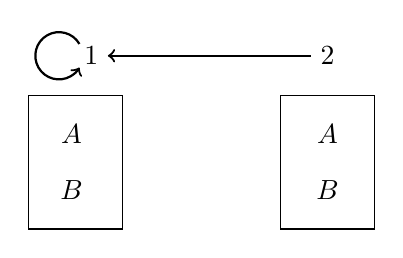
\begin{tikzpicture}
		\node (atom1) at (0,1) {1};
		\node (atom2) at (3,1) {2};
		\node (atom3) at (-0.25,0) {$A$};
		\node (atom4) at (3,0) {$\enot A$};
		\node (atom5) at (-0.25,-0.7) {$\enot B$};
		\node (atom6) at (3,-0.7) {$B$};
		\draw[->, thick] (atom1)+(-0.15,0.15) arc (-330:-30:.3);
		%\draw[->, thick] (atom2)+(0.15,-0.15) arc (-150:150:.3); 
		\draw[<-, thick] (atom1) -- (atom2);
		\draw (-0.8,-1.2) rectangle (0.4,0.5);
		\draw (2.4,-1.2) rectangle (3.6,0.5);
	\end{tikzpicture}
\end{center}
Here is how to read the interpretation off from this diagram. It contains just two worlds, 1 and 2. The arrows between the worlds indicate the accessibility relation. So 1 and 2 both access 1, but neither 1 nor 2 accesses 2. The boxes at each world let us know which atomic sentences are true at each world: $A$ is true at 1 but false at 2; $B$ is false at 1 but true at 2. You may only write an atomic sentence or the negation of an atomic sentence into one of these boxes. We can figure out what truth-values the more complex sentences get at each world from that. For example, on this interpretation all of the following sentences are true at $w_1$:
\begin{itemize}
	\item[]$A\eand\enot B$, $B\eif A$, $\ediamond A$, $\ebox\enot B$
\end{itemize}
If you don't like thinking diagrammatically, then you can also present an interpretation like this:
\begin{itemize}
	\item[$W$:]$1,2$
	\item[$R$:]$\langle 1,1\rangle, \langle 2,1\rangle$
	\item[]$\nu_{1}(A)=T, \nu_{2}(B)=F, \nu_{2}(A)=F, \nu_{2}(B)=T$
\end{itemize}
You will get the chance to cook up some interpretations of your own shortly, when we start looking at \emph{counter-interpretations}.

\section{A Semantics for System \mlK}
\label{SemanticsK}

We can now extend all of the semantic concepts of TFL to cover ML:
\factoidbox{
	\begin{itemize}
		\item  $\meta{A}_1,\meta{A}_2, \dots \meta{A}_n\therefore\meta{C}$ is \define{modally valid} iff there is no world in any interpretation at which $\meta{A}_1,\meta{A}_2, \dots \meta{A}_n$ are all true and $\meta{C}$ is false.

		\item $\meta{A}$ is a \define{modal truth} iff $\meta{A}$ is true at every world in every interpretation.

		\item $\meta{A}$ is a \define{modal contradiction} iff $\meta{A}$ is false at every world in every interpretation.

		\item $\meta{A}$ is \define{modally satisfiable} iff $\meta{A}$ is true at some world in some interpretation.
	\end{itemize}
}
(From now on we will drop the explicit `modal' qualifications, since they can be taken as read.)

We can also extend our use of $\entails$. However, we need to add subscripts again, just as we did with $\proves$. So, when we want to say that $\meta{A}_1,\meta{A}_2, \dots \meta{A}_n\therefore\meta{C}$ is valid, we will write: $\meta{A}_1,\meta{A}_2, \dots \meta{A}_n\entails_\mlK\meta{C}$. 

Let's get more of a feel for this semantics by presenting some counter-interpretations. Consider the following (false) claim:
\begin{itemize}
	\item[]
	      \begin{itemize}
		      \item[]$\enot A\entails_\mlK \enot \ediamond A$
	      \end{itemize}
\end{itemize}
In order to present a counter-interpretation to this claim, we need to cook up an interpretation which makes $\enot A$ true at some world $w$, and $\enot\ediamond A$ false at $w$. Here is one such interpretation, presented diagrammatically:
\begin{center}
	\begin{tikzpicture}
		\node (atom1) at (0,1) {1};
		\node (atom2) at (3,1) {2};
		\node (atom3) at (-0.25,0) {$\enot A$};
		\node (atom4) at (3,0) {$A$};
		\draw[->, thick] (atom1) -- (atom2);
		\draw (-0.8,-0.6) rectangle (0.4,0.5);
		\draw (2.4,-0.6) rectangle (3.6,0.5);
	\end{tikzpicture}
\end{center}
It is easy to see that this will work as a counter-interpretation for our claim. First, $\enot A$ is true at world $1$. And second, $\enot\ediamond A$ is false at $1$: $A$ is true at $2$, and $2$ is accessible from $1$. So there is some world in this interpretation where $\enot A$ is true and $\enot\ediamond A$ is false, so it is not the case that $\enot A\entails_\mlK\enot\ediamond A$.

Why did we choose the subscript \mlK? Well, it turns out that there is an important relationship between system \mlK{} and the definition of validity we have just given. In particular, we have the following two results:
\begin{itemize}
	\item If $\meta{A}_1,\meta{A}_2, \dots \meta{A}_n\proves_\mlK\meta{C}$, then $\meta{A}_1,\meta{A}_2, \dots \meta{A}_n\entails_\mlK\meta{C}$
	\item If $\meta{A}_1,\meta{A}_2, \dots \meta{A}_n\entails_\mlK\meta{C}$, then $\meta{A}_1,\meta{A}_2, \dots \meta{A}_n\proves_\mlK\meta{C}$
\end{itemize}
The first result is known as a \emph{soundness} result, since it tells us that the rules of \mlK{} are good, sound rules: if you can vindicate an argument by giving a proof for it using system \mlK, then that argument really is valid. The second result is known as a \emph{completeness} result, since it tells us that the rules of \mlK{} are broad enough to capture all of the valid arguments: if an argument is valid, then it will be possible to offer a proof in \mlK{} which vindicates it.

Now, it is one thing to state these results, quite another to prove them. However, we will not try to prove them here. But the idea behind the proof of soundness will perhaps make clearer how strict subproofs work. 

In a strict subproof, we are not allowed to make use of any information from outside the strict subproof, except what we import into the strict subproof using \ebox E. If we've assumed or proved $\ebox \meta{A}$, by \ebox E, we can used $\meta{A}$ inside a strict subproof. And in \mlK, that is the only way to import a formula into a strict subproof. So everything that can be proved inside a strict subproof must follow from formulas $\meta{A}$ where outside the strict subproof we have $\ebox \meta{A}$. Let's imagine that we are reasoning about what's true in a possible world in some interpretation. If we know that $\ebox\meta{A}$ is true in that possible world, we know that $\meta{A}$ is true in all accessible worlds. So, everything proved inside a strict subproof is true in all accessible possible worlds. That is why \ebox I is a sound rule.

\section{A Semantics for System \mlT}
\label{SemanticsT}

A few moments ago, we said that system \mlK{} is sound and complete. Where does that leave the other modal systems we looked at, namely  \mlT, \mlSfour{} and \mlSfive? Well, they are all \emph{unsound}, relative to the definition of validity we gave above. For example, all of these systems allow us to infer $A$ from $\ebox A$, even though $\ebox A\nentails_\mlK A$.

Does that mean that these systems are a waste of time? Not at all! These systems are only unsound \emph{relative to the definition of validity we gave above}. (Or to use symbols, they are unsound relative to $\entails_\mlK$.) So when we are dealing with these stronger modal systems, we just need to modify our definition of validity to fit. This is where accessibility relations come in really handy.

When we introduced the idea of an accessibility relation, we said that it could be any relation between worlds that you like: you could have it relating every world to every world, no world to any world, or anything in between. That is how we were thinking of accessibility relations in our definition of $\entails_\mlK$. But if we wanted, we could start putting some restrictions on the accessibility relation. In particular, we might insist that it has to be \emph{reflexive}:
\begin{itemize}
	\item $\forall wRww$
\end{itemize}
In English: every world accesses itself. Or in terms of relative possibility: every world is possible relative to itself. If we imposed this restriction, we could introduce a new consequence relation, $\entails_\mlT$, as follows:
\factoidbox{
	$\meta{A}_1,\meta{A}_2, \dots \meta{A}_n\entails_\mlT \meta{C}$ iff there is no world in any interpretation \emph{which has a reflexive accessibility relation}, at which $\meta{A}_1,\meta{A}_2, \dots \meta{A}_n$ are all true and $\meta{C}$ is false
}
We have attached the \mlT{} subscript to $\entails$ because it turns out that system \mlT{} is sound and complete relative to this new definition of validity:
\begin{itemize}
	\item If $\meta{A}_1,\meta{A}_2, \dots \meta{A}_n\proves_\mlT\meta{C}$, then $\meta{A}_1,\meta{A}_2, \dots \meta{A}_n\entails_\mlT\meta{C}$
	\item If $\meta{A}_1,\meta{A}_2, \dots \meta{A}_n\entails_\mlT\meta{C}$, then $\meta{A}_1,\meta{A}_2, \dots \meta{A}_n\proves_\mlT\meta{C}$
\end{itemize}
As before, we will not try to prove these soundness and completeness results. However, it is relatively easy to see how insisting that the accessibility relation must be reflexive will vindicate the R\mlT{} rule:
\factoidbox{
	\[\begin{nd}
			\have[m]{m}{\ebox \meta{A}}
			\have[\, ]{n}{\meta{A}}\rt{m}
		\end{nd}\]
}
To see this, just imagine trying to cook up a counter-interpretation to this claim:
\[
	\ebox \meta{A}\entails_\mlT \meta{A}
\]
We would need to construct a world, $w$, at which $\ebox \meta{A}$ was true, but $\meta{A}$ was false. Now, if $\ebox \meta{A}$ is true at $w$, then $\meta{A}$ must be true at every world $w$ accesses. But since the accessibility relation is reflexive, $w$ accesses $w$. So $\meta{A}$ must be true at $w$. But now $\meta{A}$ must be true \emph{and} false at $w$. Contradiction!

\section{A Semantics for \mlSfour}
\label{SemanticsS4}

How else might we tweak our definition of validity? Well, we might also stipulate that the accessibility relation has to be \emph{transitive}:
\begin{itemize}
	\item $\forall w_1\forall w_2\forall w_3 ((Rw_1w_2 \eand Rw_2w_3)\eif Rw_1w_3)$
\end{itemize}
In English: if $w_1$ accesses $w_2$, and $w_2$ accesses $w_3$, then $w_1$ accesses $w_3$. Or in terms of relative possibility: if $w_3$ is possible relative to $w_2$, and $w_2$ is possible relative to $w_1$, then $w_3$ is possible relative to $w_1$. If we added this restriction on our accessibility relation, we could introduce a new consequence relation, $\entails_\mlSfour$, as follows:
\factoidbox{
	$\meta{A}_1,\meta{A}_2, \dots \meta{A}_n\entails_\mlSfour \meta{C}$ iff there is no world in any interpretation \emph{which has a reflexive and transitive accessibility relation}, at which $\meta{A}_1,\meta{A}_2, \dots \meta{A}_n$ are all true and $\meta{C}$ is false
}
We have attached the \mlSfour{} subscript to $\entails$ because it turns out that system \mlSfour{} is sound and complete relative to this new definition of validity:
\begin{itemize}
	\item If $\meta{A}_1,\meta{A}_2, \dots \meta{A}_n\proves_\mlSfour\meta{C}$, then $\meta{A}_1,\meta{A}_2, \dots \meta{A}_n\entails_\mlSfour\meta{C}$
	\item If $\meta{A}_1,\meta{A}_2, \dots \meta{A}_n\entails_\mlSfour\meta{C}$, then $\meta{A}_1,\meta{A}_2, \dots \meta{A}_n\proves_\mlSfour\meta{C}$
\end{itemize}
As before, we will not try to prove these soundness and completeness results. However, it is relatively easy to see how insisting that the accessibility relation must be transitive will vindicate the \mlSfour{} rule:
\factoidbox{
	\[\begin{nd}
			\have[m]{m}{\ebox\meta{A}}
			\open
			\hypo[\ ]{k}{\ebox}
			\have[\ ]{n}{\ebox\meta{A}}\rfour{m}
		\end{nd}\]
}
The idea behind strict subproofs, remember, is that they are ways to prove things that must be true in all accessible worlds. So the R$\mathbf{4}$ rule means that whenever $\ebox \meta{A}$ is true, $\ebox \meta{A}$ must also be true in every accessible world. In other words, we must have $\ebox\meta{A} \entails_\mlSfour \ebox\ebox\meta{A}$.

To see this, just imagine trying to cook up a counter-interpretation to this claim:
\begin{itemize}
	\item[]$\ebox\meta{A} \entails_\mlSfour \ebox \ebox \meta{A}$
\end{itemize}
We would need to construct a world, $w_1$, at which $\ebox\meta{A}$ was true, but $\ebox \ebox \meta{A}$ was false. Now, if $\ebox \ebox \meta{A}$ is false at $w_1$, then $w_1$ must access some world, $w_2$, at which $\ebox\meta{A}$ is false. Equally, if $\ebox \meta{A}$ is false at $w_2$, then $w_2$ must access some world, $w_3$, at which $\meta{A}$ is false. We just said that $w_1$ accesses $w_2$, and $w_2$ accesses $w_3$. So since we are now insisting that the accessibility relation be transitive, $w_1$ must access $w_3$. And as $\ebox\meta{A}$ is true at $w_1$, and $w_3$ is accessible from $w_1$, it follows that $\meta{A}$ must be true at $w_3$. So $\meta{A}$ is true \emph{and} false at $w_3$. Contradiction!

\section{A Semantics for \mlSfive}
\label{SemanticsS5}

Let's put one more restriction on the accessibility relation. This time, let's insist that it must also be \emph{symmetric}:
\begin{itemize}
	\item $\forall w_1\forall w_2(Rw_1w_2 \eif Rw_2w_1)$
\end{itemize}
In English: if $w_1$ accesses $w_2$, then $w_2$ accesses $w_1$. Or in terms of relative possibility: if $w_2$ is possible relative to $w_1$, then $w_1$ is possible relative to $w_2$. Logicians call a relation that is reflexive, symmetric, and transitive an \emph{equivalence} relation. We can now define a new consequence relation, $\entails_\mlSfive $, as follows:
\factoidbox{
	$\meta{A}_1,\meta{A}_2, \dots \meta{A}_n\entails_\mlSfive  \meta{C}$ iff there is no world in any interpretation \emph{whose accessibility relation is an equivalence relation}, at which $\meta{A}_1,\meta{A}_2, \dots \meta{A}_n$ are all true and $\meta{C}$ is false
}
We have attached the \mlSfive{} subscript to $\entails$ because it turns out that system \mlSfive{} is sound and complete relative to this new definition of validity:
\begin{itemize}
	\item If $\meta{A}_1,\meta{A}_2, \dots \meta{A}_n\proves_\mlSfive \meta{C}$, then $\meta{A}_1,\meta{A}_2, \dots \meta{A}_n\entails_\mlSfive \meta{C}$
	\item If $\meta{A}_1,\meta{A}_2, \dots \meta{A}_n\entails_\mlSfive \meta{C}$, then $\meta{A}_1,\meta{A}_2, \dots \meta{A}_n\proves_\mlSfive \meta{C}$
\end{itemize}
As before, we will not try to prove these soundness and completeness results here. However, it is relatively easy to see how insisting that the accessibility relation must be an equivalence relation will vindicate the R$\mathbf{5}$ rule:
\factoidbox{
	\[\begin{nd}
			\have[m]{m}{\enot\ebox \meta{A}}
			\open
			\hypo[\ ]{k}{\ebox}
			\have[\, ]{n}{\enot\ebox\meta{A}}\rfive{m}
		\end{nd}\]
}
The rule says that if $\meta{A}$ is not necessary, i.e., false in some accessible world, it is also not necessary in any accessible prossible world, i.e., we have $\enot\ebox \meta{A} \proves_\mlSfive  \ebox\enot\ebox \meta{A}$.

To see this, just imagine trying to cook up a counter-interpretation to this claim:
\[
	\enot\ebox\meta{A} \entails_\mlSfive  \ebox \enot\ebox \meta{A}
\]
We would need to construct a world, $w_1$, at which $\enot\ebox\meta{A}$ was true, but $\ebox \enot\ebox \meta{A}$ was false. 
Now, if $\enot\ebox\meta{A}$ is true at $w_1$, then $w_1$ must access some world, $w_2$, at which $\meta{A}$ is false. Equally, if $\ebox \enot\ebox \meta{A}$ is false at $w_1$, then $w_1$ must access some world, $w_3$, at which $\enot\ebox \meta{A}$ is false. Since we are now insisting that the accessibility relation is an equivalence relation, and hence symmetric, we can infer that $w_3$ accesses $w_1$. Thus, $w_3$ accesses $w_1$, and $w_1$ accesses $w_2$. Again, since we are now insisting that the accessibility relation is an equivalence relation, and hence transitive, we can infer that $w_3$ accesses $w_2$. But earlier we said that $\enot\ebox \meta{A}$ is false at $w_3$, which implies that $\meta{A}$ is true at every world which $w_3$ accesses. So $\meta{A}$ is true \emph{and} false at $w_2$. Contradiction!

In the definition of $\entails_\mlSfive $, we stipulated that the accessibility relation must be an equivalence relation. But it turns out that there is another way of getting a notion of validity fit for \mlSfive. Rather than stipulating that the accessibility relation be an equivalence relation, we can instead stipulate that it be a \emph{universal} relation:
\begin{itemize}
	\item $\forall w_1\forall w_2Rw_1w_2$
\end{itemize}
In English: every world accesses every world. Or in terms of relative possibility: every world is possible relative to every world. Using this restriction on the accessibility relation, we could have defined $\entails_\mlSfive $ like this:
\factoidbox{
	$\meta{A}_1,\meta{A}_2, \dots \meta{A}_n\entails_\mlSfive  \meta{C}$ iff there is no world in any interpretation \emph{which has a universal accessibility relation}, at which $\meta{A}_1,\meta{A}_2, \dots \meta{A}_n$ are all true and $\meta{C}$ is false.
}
If we defined $\entails_\mlSfive $ like this, we would still get the same soundness and completeness results for \mlSfive. What does this tell us? Well, it means that if we are dealing with a notion of necessity according to which \emph{every} world is possible relative to \emph{every} world, then we should use \mlSfive. What is more, most philosophers assume that the notions of necessity that they are most concerned with, like \emph{logical necessity} and \emph{metaphysical necessity}, are of exactly this kind. So \mlSfive{} is the modal system that most philosophers use most of the time.

\practiceproblems

\problempart
Present counter-interpretations to the following false claims:
\begin{earg}
	\item $\enot P \entails_\mlK \enot\ediamond P$
	\item $\ebox(P \eor Q)\entails_\mlK \ebox P \eor \ebox Q$
	\item $\entails_\mlK \enot \ebox (A\eand \enot A)$
	\item $\ebox A\entails_\mlK A$
\end{earg}

\problempart
Present counter-interpretations to the following false claims:
\begin{earg}
	\item $\ediamond A\entails_\mlSfour \ebox\ediamond A$
	\item $\ediamond A, \ebox (\ediamond A \eif B)\entails_\mlSfour\ebox B$
\end{earg}

\problempart
Present counter-interpretations to the following false claims:
\begin{earg}
	\item $\ebox (M\eif O),\ediamond M\entails_\mlT O$
	\item $\ebox A\entails_\mlT \ebox \ebox A$
\end{earg}

\section*{Further reading}

Modal logic is a large subfield of logic. We have only scratched the surface. If you want to learn more about modal logic, here are some textbooks you might consult.

\begin{itemize}
	\item Hughes, G. E., \& Cresswell, M. J. (1996). \emph{A New Introduction to Modal Logic}, Oxford: Routledge.
	\item Priest, G. (2008). \emph{An Introduction to Non-Classical Logic}, 2nd ed., Cambridge: Cambridge University Press.
	\item Garson, J. W. (2013). \emph{Modal Logic for Philosophers}, 2nd ed., Cambridge: Cambridge University Press.
\end{itemize}

None of these authors formulate their modal proof systems in quite the way we did, but the closest formulation is given by Garson.

%%!TEX root = forallxyyc.tex
\part{Metateoria}
\label{ch.normalform}
\addtocontents{toc}{\protect\mbox{}\protect\hrulefill\par}

\chapter{Formas normais e expressividade}


\section{Disjunctive Normal Form}\label{s:DNFDefined}

Sometimes it is useful to consider sentences of a particularly simple form. For instance, we might consider sentences in which $\enot$ only attaches to atomic sentences, or those which are combinations of atomic sentences and negated atomic sentences using only $\eand$.  A relatively general but still simple form is that where a sentence is a disjunction of conjunctions of atomic or negated atomic sentences.  When such a sentence is constructed, we start with atomic sentences, then (perhaps) attach negations, then (perhaps) combine using $\eand$, and finally (perhaps) combine using~$\eor$. 

Let's say that a sentence is in \define{disjunctive normal form} \emph{iff} it meets all of the following conditions:
	\begin{earg}
		\item[(\textsc{dnf1})] No connectives occur in the sentence other than negations, conjunctions and disjunctions;
		\item[(\textsc{dnf2})] Every occurrence of negation has minimal scope (i.e.\ any `$\enot$' is immediately followed by an atomic sentence);
		\item[(\textsc{dnf3})] No disjunction occurs within the scope of any conjunction.
	\end{earg}
\newglossaryentry{disjunctive normal form}{
  name = disjunctive normal form (DNF),
  text = disjunctive normal form,
  description = {a sentence which is a disjunction of conjunctions of atomic sentences or negated atomic sentences}
}
So, here are are some sentences in disjunctive normal form:
\begin{align*}
  & A \\
  & (A \eand \lnot B \eand C)\\
  & (A \eand B) \eor (A \eand \enot B)\\
  & (A \eand B) \eor (A \eand  B \eand C \eand \enot D \eand \enot E)\\
  & A \eor (C \eand \enot P_{234} \eand P_{233} \eand Q) \eor \enot B
\end{align*}
Note that we have here broken one of the maxims of this book and \emph{temporarily} allowed ourselves to employ the relaxed bracketing-conventions that allow conjunctions and disjunctions to be of arbitrary length. These conventions make it easier to see when a sentence is in disjunctive normal form. We will continue to help ourselves to these relaxed conventions, without further comment.

To further illustrate the idea of disjunctive normal form, we will introduce some more notation. We write `$\pm\meta{A}$' to indicate that $\meta{A}$ is an atomic sentence which may or may not be prefaced with an occurrence of negation. Then a sentence in disjunctive normal form has the following shape:
	$$(\pm \meta{A}_1 \land \ldots \land \pm \meta{A}_i) \lor (\pm \meta{A}_{i+1} \land \ldots \land \pm\meta{A}_j) \lor \ldots \lor (\pm\meta{A}_{m+1} \land \ldots \land \pm \meta{A}_n)$$
We now know what it is for a sentence to be in disjunctive normal form. The result that we are aiming at is:
	\factoidbox{\label{thm:dnf}\textbf{Disjunctive Normal Form Theorem.} For any sentence, there is a logically equivalent sentence in disjunctive normal form.
	}
Henceforth, we will abbreviate `Disjunctive Normal Form' by `DNF'. 


\section{Proof of DNF Theorem via truth tables}
\label{s:DNFTruthTable}

Our first proof of the DNF Theorem employs truth tables. We will first illustrate the technique for finding an equivalent sentence in DNF, and then turn this illustration into a rigorous proof. 

Let's suppose we have some sentence, $\meta{S}$, which contains three atomic sentences, `$A$', `$B$' and `$C$'. The very first thing to do is fill out a complete truth table for $\meta{S}$. Maybe we end up with this:
\begin{center}
\begin{tabular}{c c c | c}
$A$ & $B$ & $C$ & $\meta{S}$\\
\hline
 T & T & T & T \\
 T & T & F & F \\
 T & F & T & T \\
 T & F & F & F \\
 F & T & T & F \\
 F & T & F & F \\
 F & F & T & T \\
 F & F & F & T
\end{tabular}
\end{center}
%Now, consider a sentence, whose only connectives are negations and conjunctions, where no connective occurs within the scope of any negation, e.g.:
%	$$A \eand \enot B \eand C$$
%This sentence is true when, and only when, `$A$' is true, `$B$' is false and `$C$' is true. Similarly, the sentence:
%	$$\enot A \eand \enot B \eand C$$
%this is true when, and only when, `$A$' is false, `$B$' is false and `$C$' is true. 
%
%A disjunction is true when, and only when, at least one of the disjuncts is true. So if we write down a disjunction of sentences of the above form, perhaps
%	$$(A \eand \enot B \eand C) \eor (\enot A \eand \enot B \eand C)$$
%then it will be true on exactly \emph{two} lines of the truth table which describes all possible valuations of `$A$', `$B$' and `$C$'. 
%
As it happens, $\meta{S}$ is true on four lines of its truth table, namely lines 1, 3, 7 and 8. Corresponding to each of those lines, we will write down four sentences, whose only connectives are negations and conjunctions, where every negation has minimal scope:
	\begin{earg}
		\item  `$A \eand B \eand C$'\hfill which is true on line 1 (and only then)
		\item `$A \eand \enot B \eand C$' \hfill which is true on line 3 (and only then)
		\item `$\enot A \eand \enot B \eand C$' \hfill which is true on line 7 (and only then)
		\item `$\enot A \eand \enot B \eand \enot C$' \hfill which is true on line 8 (and only then)
	\end{earg}
We now combine all of these conjunctions using~$\eor$, like so:
$$(A \eand B \eand C) \eor (A \eand \enot B \eand C) \eor (\enot A \eand \enot B \eand C) \eor (\enot A \eand \enot B \eand \enot C)$$
This gives us a sentence in DNF which is true on exactly those lines where one of the disjuncts is true, i.e.\ it is true on (and only on) lines 1, 3, 7, and 8. So this sentence has exactly the same truth table as $\meta{S}$. So we have a sentence in DNF that is logically equivalent to $\meta{S}$, which is exactly what we wanted!

Now, the strategy that we just adopted did not depend on the specifics of $\meta{S}$; it is perfectly general. Consequently, we can use it to obtain a simple proof of the DNF Theorem.

Pick any arbitrary sentence, $\meta{S}$, and let $\meta{A}_1, \ldots, \meta{A}_n$ be the atomic sentences that occur in $\meta{S}$. To obtain a sentence in DNF that is logically equivalent $\meta{S}$, we consider $\meta{S}$'s truth table. There are two cases to consider:
	\begin{enumerate}
		\item \emph{$\meta{S}$ is false on every line of its truth table.} Then, $\meta{S}$ is a contradiction. In that case, the contradiction $(\meta{A}_1 \eand \enot \meta{A}_1)$ is in DNF and logically equivalent to~$\meta{S}$. 
	
		\item \emph{$\meta{S}$ is true on at least one line of its truth table.}
		For each line $i$ of the truth table, let $\meta{B}_i$ be a conjunction of the form 
		$$(\pm\meta{A}_1 \land \ldots \land \pm\meta{A}_n)$$
		where the following rules determine whether or not to include a negation in front of each atomic sentence:
			\begin{align*}
				\meta{A}_m\text{ is a conjunct of }\meta{B}_i&\emph{ iff }\meta{A}_m\text{ is true on line }i\\
				\enot\meta{A}_m\text{ is a conjunct of }\meta{B}_i&\emph{ iff }\meta{A}_m\text{ is false on line }i
			\end{align*}
		Given these rules, $\meta{B_i}$ is true on (and only on) line $i$ of the truth table which considers all possible valuations of $\meta{A}_1, \ldots, \meta{A}_n$ (i.e.\ $\meta{S}$'s truth table). 
		
		Next, let $i_1$, $i_2$, \dots, $i_m$ be the numbers of the lines of the truth table where $\meta{S}$ is \emph{true}. Now let $\meta{D}$ be the sentence:
		$$\meta{B}_{i_1} \eor \meta{B}_{i_2} \eor \ldots \eor \meta{B}_{i_m}$$
		Since $\meta{S}$ is true on at least one line of its truth table, $\meta{D}$ is indeed well-defined; and in the limiting case where $\meta{S}$ is true on exactly one line of its truth table, $\meta{D}$ is just $\meta{B}_{i_1}$, for some $i_1$.
		
		By construction, $\meta{D}$ is in DNF. Moreover, by construction, for each line~$i$ of the truth table: $\meta{S}$ is true on line $i$ of the truth table \emph{iff} one of $\meta{D}$'s disjuncts (namely, $\meta{B_i}$) is true on, and only on, line $i$. Hence $\meta{S}$ and $\meta{D}$ have the same truth table, and so are logically equivalent.
	\end{enumerate}
	These two cases are exhaustive and, either way, we have a sentence in DNF that is logically equivalent to $\meta{S}$.

So we have proved the DNF Theorem. Before we say any more, though, we should immediately flag that we are hereby returning to the austere definition of a (TFL) sentence, according to which we can assume that any conjunction has exactly two conjuncts, and any disjunction has exactly two disjuncts.


\section{Conjunctive Normal Form}
\label{s:CNF}

So far in this chapter, we have discussed \emph{disjunctive} normal form. It may not come as a surprise to hear that there is also such a thing as \emph{conjunctive normal form} (CNF).

The definition of CNF is exactly analogous to the definition of DNF. So, a sentence is in CNF \emph{iff} it meets all of the following conditions:
	\begin{earg}
		\item[(\textsc{cnf1})] No connectives occur in the sentence other than negations, conjunctions and disjunctions;
		\item[(\textsc{cnf2})] Every occurrence of negation has minimal scope;
		\item[(\textsc{cnf3})] No conjunction occurs within the scope of any disjunction. 
	\end{earg}
\newglossaryentry{conjunctive normal form}{
  name = conjunctive normal form (DNF),
  text = conjunctive normal form,
  description = {a sentence which is a conjunction of disjunctions of atomic sentences or negated atomic sentences}
}
Generally, then, a sentence in CNF looks like this
	$$(\pm \meta{A}_1 \lor \ldots \lor \pm \meta{A}_i) \land (\pm \meta{A}_{i+1} \lor \ldots \lor \pm\meta{A}_j) \land \ldots \land (\pm\meta{A}_{m+1} \lor\ldots \lor \pm \meta{A}_n)$$
where each $\meta{A}_k$ is an atomic sentence.

We can now prove another normal form theorem:
	\factoidbox{\label{thm:cnf}\textbf{Conjunctive Normal Form Theorem.} For any sentence, there is a logically equivalent sentence in conjunctive normal form.}

        
	Given a TFL sentence, $\meta{S}$, we begin by writing down the complete truth table for $\meta{S}$.
	
	If $\meta{S}$ is \emph{true} on every line of the truth table, then $\meta{S}$ and $(\meta{A}_1 \eor \enot \meta{A}_1)$ are logically equivalent.
	
	If $\meta{S}$ is \emph{false} on at least one line of the truth table then, for every line on the truth table where $\meta{S}$ is false, write down a disjunction $(\pm\meta{A}_1 \eor \ldots \eor \pm\meta{A}_n)$ which is \emph{false} on (and only on) that line. Let $\meta{C}$ be the conjunction of all of these disjuncts; by construction, $\meta{C}$ is in CNF and $\meta{S}$ and $\meta{C}$ are logically equivalent.

\practiceproblems
\problempart
\label{pr.DNF}
Consider the following sentences:
	\begin{earg}
		\item $(A \eif \enot B)$
		\item $\enot (A \eiff B)$
		\item $(\enot A \eor \enot (A \eand B))$
		\item $(\enot (A \eif B ) \eand (A \eif C))$
		\item $(\enot (A \eor B) \eiff ((\enot C \eand \enot A) \eif \enot B))$
		\item $((\enot (A \eand \enot B) \eif C) \eand \enot (A \eand D))$
	\end{earg}
        For each sentence, find a logically equivalent sentence in DNF and one in CNF.
        
\section{The expressive adequacy of TFL}

Of our connectives, $\enot$ attaches to a single sentences, and the others all combine exactly two sentences. We may also introduce the idea of an $n$-place connective. For example, we could consider a three-place connective, `$\heartsuit$', and stipulate that it is to have the following characteristic truth table:
\begin{center}
\begin{tabular}{c c c | c}
$A$ & $B$ & $C$ & $\heartsuit(A,B,C)$\\
\hline
 T & T & T & F \\
 T & T & F & T \\
 T & F & T & T \\
 T & F & F & F \\
 F & T & T & F \\
 F & T & F & T \\
 F & F & T & F \\
 F & F & F & F
\end{tabular}
\end{center}
Probably this new connective would not correspond with any natural English expression (at least not in the way that `$\eand$' corresponds with `and'). But a question arises: if we wanted to employ a connective with this characteristic truth table, must we add a \emph{new} connective to TFL? Or can we get by with the connectives we \emph{already have}?

Let us make this question more precise. Say that some connectives are \define{jointly expressively adequate} \emph{iff}, for any possible truth table, there is a sentence containing only those connectives with that truth table.

\newglossaryentry{expressively adequate}{
  name = {expressive adequacy},
  text = {expressively adequate},
  description = {property of a collection of connectives which holds iff every possible truth table is the truth table of a sentence involving only those connectives}}

The general point is, when we are armed with some jointly expressively adequate connectives, no characteristic truth table lies beyond our grasp. And in fact, we are in luck.
	\factoidbox{\label{thm:ExpressiveAdequacy}\textbf{Expressive Adequacy Theorem.}
The connectives of TFL are jointly expressively adequate. Indeed, the following pairs of connectives are jointly expressively adequate:
\begin{earg}
\item\label{expressive:eor} `$\enot$' and `$\eor$'
\item\label{expressive:eand} `$\enot$' and `$\eand$'
\item\label{expressive:eif} `$\enot$' and `$\eif$'
\end{earg}}

Given any truth table, we can use the method of proving the DNF Theorem (or the CNF Theorem) via truth tables, to write down a scheme which has the same truth table. For example, employing the truth table method for proving the DNF Theorem, we find that the following scheme has the same characteristic truth table as $\heartsuit(A,B,C)$, above:
		$$(A \eand B \eand \enot C) \eor (A \eand \enot B \eand C) \eor (\enot A \eand B \eand \enot C)$$			
It follows that the connectives of TFL are jointly expressively adequate. We now prove each of the subsidiary results.
	
\emph{Subsidiary Result \ref{expressive:eor}: expressive adequacy of `$\enot$' and `$\eor$'.} Observe that the scheme that we generate, using the truth table method of proving the DNF Theorem, will only contain the connectives `$\enot$', `$\eand$' and `$\eor$'. So it suffices to show that there is an equivalent scheme which contains only `$\enot$' and `$\eor$'. To show do this, we simply consider that
		\begin{align*}
		(\meta{A} \eand \meta{B}) & \text{\quad and \quad} \enot(\enot \meta{A} \eor\enot \meta{B})
		\end{align*}
		are logically equivalent.

\emph{Subsidiary Result \ref{expressive:eand}: expressive adequacy of `$\enot$' and `$\eand$'.} Exactly as in Subsidiary Result~\ref{expressive:eor}, making use of the fact that
		\begin{align*}
		(\meta{A} \eor \meta{B}) & \text{\quad and \quad}\enot(\enot \meta{A} \eand\enot \meta{B})
		\end{align*}
are logically equivalent.

\emph{Subsidiary Result \ref{expressive:eif}: expressive adequacy of `$\enot$' and `$\eif$'.} Exactly as in Subsidiary Result~\ref{expressive:eor}, making use of these equivalences instead:
		\begin{align*}
		(\meta{A} \eor \meta{B}) &\text{\quad and \quad} (\enot \meta{A} \eif \meta{B})\\
		(\meta{A} \eand \meta{B}) &\text{\quad and \quad} \enot(\meta{A} \eif \enot\meta{B})
		\end{align*}
Alternatively, we could simply rely upon one of the other two subsidiary results, and (repeatedly) invoke only one of these two equivalences.

In short, there is never any \emph{need} to add new connectives to TFL. Indeed, there is already some redundancy among the connectives we have: we could have made do with just two connectives, if we had been feeling really austere.

\section{Individually expressively adequate connectives}

In fact, some two-place connectives are \emph{individually} expressively adequate. These connectives are not standardly included in TFL, since they are rather cumbersome to use. But their existence shows that, if we had wanted to, we could have defined a truth-functional language that was expressively adequate, which contained only a single primitive connective.

The first such connective we will consider is `$\uparrow$', which has the following characteristic truth table. 
\begin{center}
\begin{tabular}{c c | c}
$\meta{A}$ & $\meta{B}$ & $\meta{A} \mathrel{\uparrow} \meta{B}$\\
\hline
 T & T & F \\
 T & F & T \\
 F & T & T  \\
 F & F & T
\end{tabular}
\end{center}
 This is often called `the Sheffer stroke', after Henry Sheffer, who used it to show how to reduce the number of logical connectives in Russell and Whitehead's \emph{Principia Mathematica}.\footnote{Sheffer, `A Set of Five Independent Postulates for Boolean Algebras, with application to logical constants,' (1913, \emph{Transactions of the American Mathematical Society} 14.4)} (In fact, Charles Sanders Peirce had anticipated Sheffer by about 30 years, but never published his results.)\footnote{See Peirce, `A Boolian Algebra with One Constant', which dates to c.1880; and Peirce's \emph{Collected Papers}, 4.264--5.} It is quite common, as well, to call it `nand', since its characteristic truth table is the negation of the truth table for `$\eand$'.
\factoidbox{\label{prop:upexpressive}`$\uparrow$' is expressively adequate all by itself.}

The Expressive Adequacy Theorem tells us that `$\enot$' and `$\eor$' are jointly expressively adequate. So it suffices to show that, given any scheme which contains only those two connectives, we can rewrite it as a logically equivalent scheme which contains only `$\uparrow$'. As in the proof of the subsidiary cases of the Expressive Adequacy Theorem, then, we simply apply the following equivalences:
		\begin{align*}
			\enot \meta{A} &\text{\quad and \quad} (\meta{A} \uparrow \meta{A})\\
			(\meta{A} \eor \meta{B}) & \text{\quad and \quad} ((\meta{A} \uparrow \meta{A}) \uparrow (\meta{B} \uparrow \meta{B}))
		\end{align*}
to the Subsidiary Result~\ref{expressive:eor}.

Similarly, we can consider the connective `$\downarrow$':
\begin{center}
\begin{tabular}{c c | c}
$\meta{A}$ & $\meta{B}$ & $\meta{A} \mathrel{\downarrow} \meta{B}$\\
\hline
 T & T & F \\
 T & F & F  \\
 F & T & F  \\
 F & F & T
\end{tabular}
\end{center}
This is sometimes called the `Peirce arrow' (Peirce himself called it `ampheck'). More often, though, it is called `nor', since its characteristic truth table is the negation of `$\eor$', that is, of `neither \dots{} nor \dots'.
	\factoidbox{
	`$\downarrow$' is expressively adequate all by itself. }

As in the previous result for $\uparrow$, although invoking the equivalences:
		\begin{align*}
			\enot \meta{A} &\text{\quad and \quad} (\meta{A} \downarrow \meta{A})\\
			(\meta{A} \eand \meta{B}) & \text{\quad and \quad} ((\meta{A} \downarrow \meta{A}) \downarrow (\meta{B} \downarrow \meta{B}))
		\end{align*}
and Subsidiary Result~\ref{expressive:eand}.


\section{Failures of expressive adequacy}

In fact, the \emph{only} two-place connectives which are individually expressively adequate are `$\uparrow$' and `$\downarrow$'. But how would we show this? More generally, how can we show that some connectives are \emph{not} jointly expressively adequate? 
 
The obvious thing to do is to try to find some truth table which we \emph{cannot} express, using just the given connectives. But there is a bit of an art to this.

To make this concrete, let's consider the question of whether `$\eor$' is expressively adequate all by itself. After a little reflection, it should be clear that it is not. In particular, it should be clear that any scheme which only contains disjunctions cannot have the same truth table as negation, i.e.:
				\begin{center}
				\begin{tabular}{c | c}
				$\meta{A}$ & $\enot \meta{A}$\\
				\hline
				 T & F \\
				 F & T
				\end{tabular}
				\end{center}
The intuitive reason, why this should be so, is simple: the top line of the desired truth table needs to have the value False; but the top line of any truth table for a scheme which \emph{only} contains $\eor$ will always be True. The same is true for $\eand$, $\eif$, and $\eiff$.
 	\factoidbox{
		`$\eor$', `$\eand$', `$\eif$', and `$\eiff$' are not expressively adequate by themselves.}

In fact, the following is true:
        
\factoidbox{The \emph{only} two-place connectives that are expressively adequate by themselves are `$\uparrow$' and `$\downarrow$'. }

This is of course harder to prove than for the primitive connectives. For instance, the ``exclusive or'' connective does not have a T in the first line of its characteristic truth table, and so the method used above no longer suffices to show that it cannot express all truth tables.  It is also harder to show that, e.g., `$\eiff$' and `$\enot$' \emph{together} are not expressively adequate.


\chapter{Correção}\label{ch:Soundness}

In this chapter we relate TFL's semantics to its natural deduction \emph{proof system} (as defined in Part~\ref{ch.NDTFL}). We will prove that the formal proof system is safe: you can only prove sentences from premises from which they actually follow.
Intuitively, a formal proof system is sound iff it does not allow you to prove any invalid arguments. This is obviously a highly desirable property. It tells us that our proof system will never lead us astray. Indeed, if our proof system were not sound, then we would not be able to trust our proofs. The aim of this chapter is to prove that our proof system is sound.

Let's make the idea more precise. We'll abbreviate a list of sentences using the greek letter $\Gamma$ (`gamma'). A formal proof system is \define{sound} (relative to a given semantics) \emph{iff}, whenever there is a formal proof of $\meta{C}$ from assumptions among $\Gamma$, then $\Gamma$ genuinely entails $\meta{C}$ (given that semantics). Otherwise put, to prove that TFL's proof system is sound, we need to prove the following

\begin{factoidboxe}\textbf{Soundness Theorem.} For any sentences $\Gamma$ and $\meta{C}$: if $\Gamma\proves\meta{C}$, then $\Gamma \entails\meta{C}$
\end{factoidboxe}

To prove this, we will check each of the rules of TFL's proof system individually. We want to show that no application of those rules ever leads us astray. Since a proof just involves repeated application of those rules, this will show that no proof ever leads us astray. Or at least, that is the general idea.

To begin with, we must make the idea of `leading us astray' more precise. Say that a line of a proof is \define{shiny} iff the assumptions on which that line depends tautologically entail the sentence on that line.\footnote{The word `shiny' is not standard among logicians.} To illustrate the idea, consider the following:
	\begin{proof}
		\hypo{fgh}{F\eif(G\eand H)}
		\open
			\hypo{f}{F}
			\have{gh}{G \eand H}\ce{fgh,f}
			\have{g}{G}\ae{gh}
		\close
		\have{fg}{F \eif G}\ci{f-g}
	\end{proof}\noindent\noindent
Line $1$ is shiny iff $F \eif (G \eand H) \entails F \eif (G \eand H)$. You should be easily convinced that line $1$ is, indeed, shiny! Similarly, line $4$ is shiny iff $F \eif (G \eand H), F \entails G$. Again, it is easy to check that line $4$ is shiny. As is every line in this TFL-proof. We want to show that this is no coincidence. That is, we want to prove:
	\begin{factoidboxe}\textbf{Shininess Lemma.}
		Every line of every TFL-proof is shiny.
	\end{factoidboxe}\noindent
Then we will know that we have never gone astray, on any line of a proof. Indeed, given the Shininess Lemma, it will be easy to prove the Soundness Theorem:

\emph{Proof.} Suppose $\Gamma \proves \meta{C}$. Then there is a TFL-proof, with $\meta{C}$ appearing on its last line, whose only undischarged assumptions are among $\Gamma$. The Shininess Lemma tells us that every line on every TFL-proof is shiny. So this last line is shiny, i.e.\ $\Gamma \entails \meta{C}$. QED

It remains to prove the Shininess Lemma. 

To do this, we observe that every line of any TFL-proof is obtained by applying some rule. So what we want to show is that no application of a rule of TFL's proof system will lead us astray. More precisely, say that a rule of inference is \define{rule-sound} \emph{iff} for all TFL-proofs, if we obtain a line on a TFL-proof by applying that rule, and every earlier line in the TFL-proof is shiny, then our new line is also shiny. What we need to show is that \emph{every} rule in TFL's proof system is rule-sound. 

We will do this in the next section. But having demonstrated the rule-soundness of every rule, the Shininess Lemma will follow immediately:

\emph{Proof.} Fix any line, line $n$, on any TFL-proof. The sentence written on line $n$ must be obtained using a formal inference rule which is rule-sound. This is to say that, if every earlier line is shiny, then line $n$ itself is shiny. Hence, by strong induction on the length of TFL-proofs, every line of every TFL-proof is shiny. QED

Note that this proof appeals to a principle of strong induction on the length of TFL-proofs. This is the first time we have seen that principle, and you should pause to confirm that it is, indeed, justified.

It remains to show that every rule is rule-sound. This is not difficult, but it is time-consuming, since we need to check each rule individually, and TFL's proof system has plenty of rules! To speed up the process marginally, we will introduce a convenient abbreviation: `$\Delta_i$' (`delta') will abbreviate the assumptions (if any) on which line $i$ depends in our TFL-proof (context will indicate which TFL-proof we have in mind).

\begin{factoidboxe}Introducing an assumption is rule-sound.
\end{factoidboxe}

If $\meta{A}$ is introduced as an assumption on line $n$, then $\meta{A}$ is among $\Delta_n$, and so $\Delta_n \entails \meta{A}$.

\begin{factoidboxe}$\eand$I is rule-sound.
\end{factoidboxe}

\emph{Proof.} Consider any application of $\eand$I in any TFL-proof, i.e., something like:
\begin{proof}
	\have[i]{a}{\meta{A}}
	\have[j]{b}{\meta{B}}
	\have[n]{c}{\meta{A}\eand\meta{B}} \ai{a, b}
\end{proof}\noindent
To show that $\eand$I is rule-sound, we assume that every line before line $n$ is shiny; and we aim to show that line $n$ is shiny, i.e.\ that $\Delta_n \entails \meta{A} \eand \meta{B}$. 

So, let $v$ be any valuation that makes all of $\Delta_{n}$ true. 

We first show that $v$ makes $\meta{A}$ true. To prove this, note that all of $\Delta_i$ are among $\Delta_{n}$. By hypothesis, line $i$ is shiny. So any valuation that makes all of $\Delta_i$ true makes $\meta{A}$ true. Since $v$ makes all of $\Delta_i$ true, it makes $\meta{A}$ true too.

We can similarly see that $v$ makes $\meta{B}$ true. 

So $v$ makes $\meta{A}$ true and $v$ makes $\meta{B}$ true. Consequently, $v$ makes $\meta{A}\eand\meta{B}$ true. So any valuation that makes all of the sentences among $\Delta_{n}$ true also makes $\meta{A} \eand \meta{B}$ true. That is: line $n$ is shiny. QED


All of the remaining lemmas establishing rule-soundness will have, essentially, the same structure as this one did. 

\begin{factoidboxe}$\eand$E is rule-sound.
\end{factoidboxe}

\emph{Proof.}
	Assume that every line before line $n$ on some TFL-proof is shiny, and that $\eand$E is used on line $n$. So the situation is:
		   \begin{proof}
			   \have[i]{ab}{\meta{A}\eand\meta{B}}
			   \have[n]{a}{\meta{A}} \ae{ab}
		   \end{proof}\noindent
(or perhaps with $\meta{B}$ on line $n$ instead; but similar reasoning will apply in that case). Let $v$ be any valuation that makes all of $\Delta_{n}$ true. Note that all of $\Delta_i$ are among $\Delta_{n}$. By hypothesis, line $i$ is shiny. So any valuation that makes all of $\Delta_i$ true makes $\meta{A}\eand\meta{B}$ true. So $v$ makes $\meta{A}\eand\meta{B}$ true, and hence makes $\meta{A}$ true. So $\Delta_{n} \entails \meta{A}$. QED


\begin{factoidboxe}$\eor$I is rule-sound.
\end{factoidboxe}

We leave this as an exercise.

\begin{factoidboxe}$\eor$E is rule-sound.
\end{factoidboxe}

\emph{Proof.}
	Assume that every line before line $n$ on some TFL-proof is shiny, and that $\eand$E is used on line $n$. So the situation is:
   \begin{proof}
	   \have[m]{aob}{\meta{A}\eor\meta{B}}
	   \open
		   \hypo[i]{a}{\meta{A}} %\by{want \meta{C}}{}
		   \have[j]{c1}{\meta{C}}
	   \close
	   \open
		   \hypo[k]{b}{\meta{B}} %\by{want \meta{C}}{}
		   \have[l]{c2}{\meta{C}}
	   \close
	   \have[n]{ab}{\meta{C}}\oe{aob, a-c1,b-c2}
   \end{proof}\noindent
Let $v$ be any valuation that makes all of $\Delta_{n}$ true. Note that all of $\Delta_m$ are among $\Delta_{n}$. By hypothesis, line $m$ is shiny. So any valuation that makes $\Delta_{n}$ true makes $\meta{A} \eor \meta{B}$ true. So in particular, $v$ makes $\meta{A} \eor \meta{B}$ true, and hence either $v$ makes $\meta{A}$ true, or $v$ makes $\meta{B}$ true. We now reason through these two cases:
   \begin{ebullet}
	   \item[\emph{Case 1: $v$ makes $\meta{A}$ true.}] All of $\Delta_i$ are among $\Delta_{n}$, with the possible exception of $\meta{A}$. Since $v$ makes all of $\Delta_{n}$ true, and also makes $\meta{A}$ true,  $v$ makes all of $\Delta_i$ true. Now, by assumption, line $j$ is shiny; so $\Delta_{j} \entails \meta{C}$. But the sentences $\Delta_i$ are just the sentences $\Delta_{j}$, so $\Delta_i \entails \meta{C}$. So, any valuation that makes all of $\Delta_i$ true makes $\meta{C}$ true. But $v$ is just such a valuation. So $v$ makes $\meta{C}$ true. 
	   \item[\emph{Case 2: $v$ makes $\meta{B}$ true.}] Reasoning in exactly the same way, considering lines $k$ and $l$, $v$ makes $\meta{C}$ true.
	   \end{ebullet}
Either way, $v$ makes $\meta{C}$ true. So $\Delta_n \entails \meta{C}$.
QED


\begin{factoidboxe}
	$\enot$E is rule-sound.
\end{factoidboxe}

\emph{Proof.}
	Assume that every line before line $n$ on some TFL-proof is shiny, and that $\enot$E is used on line $n$. So the situation is:
\begin{proof}
   \have[i]{i}{\meta{A}} 
   \have[j]{j}{\enot\meta{A}}
   \have[n]{nb}{\ered}\ri{i, j}
\end{proof}\noindent
Note that all of $\Delta_i$ and all of $\Delta_j$ are among $\Delta_{n}$. By hypothesis, lines $i$ and $j$ are shiny. So any valuation which makes all of $\Delta_{n}$ true would have to make both $\meta{A}$ and $\enot\meta{A}$ true. But no valuation can do that. So no valuation makes all of $\Delta_{n}$ true. So $\Delta_{n} \entails \ered$, vacuously.
QED

\begin{factoidboxe}
	X is rule-sound.
\end{factoidboxe}

We leave this as an exercise.

\begin{factoidboxe}
	$\enot$I is rule-sound.
\end{factoidboxe}

\emph{Proof.}
	Assume that every line before line $n$ on some TFL-proof is shiny, and that $\enot$I is used on line $n$. So the situation is:
\begin{proof}
   \open
	   \hypo[i]{a}{\meta{A}}
	   \have[j]{b}{\ered}
   \close
   \have[n]{na}{\enot\meta{A}}\ni{a-b}
\end{proof}\noindent
Let $v$ be any valuation that makes all of $\Delta_{n}$ true. Note that all of $\Delta_{n}$ are among $\Delta_i$, with the possible exception of $\meta{A}$ itself. By hypothesis, line $j$ is shiny. But no valuation can make `$\ered$' true, so no valuation can make all of $\Delta_{j}$ true. Since the sentences $\Delta_i$ are just the sentences $\Delta_{j}$, no valuation can make all of $\Delta_i$ true. Since $v$ makes all of $\Delta_{n}$ true, it must therefore make $\meta{A}$ false, and so make $\enot \meta{A}$ true. So $\Delta_n \entails \enot \meta{A}$.
QED


\begin{factoidboxe}\label{lem:LastRuleSound} IP, $\eif$I,  $\eif$E, $\eiff$I, and $\eiff$E are all rule-sound.
\end{factoidboxe}

We leave these as exercises.

This establishes that all the basic rules of our proof system are rule-sound. Finally, we show:

\begin{factoidboxe}All of the derived rules of our proof system are rule-sound.
\end{factoidboxe}

\emph{Proof.}
	Suppose that we used a derived rule to obtain some sentence, $\meta{A}$, on line $n$ of some TFL-proof, and that every earlier line is shiny. Every use of a derived rule can be replaced (at the cost of long-windedness) with multiple uses of basic rules. That is to say, we could have used basic rules to write $\meta{A}$ on some line $n + k$, without introducing any further assumptions. So, applying our individual results that all basic rules are rule-sound several times ($k + 1$ times, in fact), we can see that line $n+k$ is shiny. Hence the derived rule is rule-sound. 
QED
	

And that's that! We have shown that every rule---basic or otherwise---is rule-sound, which is all that we required to establish the Shininess Lemma, and hence the Soundness Theorem.

But it might help to round off this chapter if we repeat my informal explanation of what we have done. A formal proof is just a sequence---of arbitrary length---of applications of rules. We have shown that any application of any rule will not lead you astray. It follows (by induction)that no formal proof will lead you astray. That is: our proof system is sound. 

\practiceproblems

\problempart
\label{pr.Soundness}
Complete the Lemmas left as exercises in this chapter. That is, show that the following are rule-sound:
	\begin{earg}
		\item $\eor$I. (\emph{Hint}: this is  similar to the case of $\eand$E.)
		\item X. (\emph{Hint}: this is similar to the case of $\enot$E.)
		\item $\eif$I. (\emph{Hint}: this is similar to $\eor$E.)
		\item $\eif$E.
		\item IP. (\emph{Hint}: this is similar to the case of $\enot$I.)
	\end{earg}



\appendix
%\part*{Apêndices}
%\addcontentsline{toc}{part}{Appendices}
%\addtocontents{toc}{\protect\mbox{}\protect\hrulefill\par}

%%!TEX root = forallxyyc.tex

\chapter{Notação simbólica}
\label{app.notation}

\section{Alternative nomenclature}

\paragraph{Truth-functional logic.} TFL goes by other names. Sometimes it is called \emph{sentential logic}, because it deals fundamentally with sentences. Sometimes it is called \emph{propositional logic}, on the idea that it deals fundamentally with propositions. We have stuck with \emph{truth-functional logic}, to emphasize the fact that it deals only with assignments of truth and falsity to sentences, and that its connectives are all truth-functional.

\paragraph{First-order logic.} FOL goes by other names. Sometimes it is called \emph{predicate logic}, because it allows us to apply  predicates to objects. Sometimes it is called \emph{quantified logic}, because it makes use of quantifiers.

\paragraph{Formulas.} Some texts call formulas \emph{well-formed formulas}. Since `well-formed formula' is such a long and cumbersome phrase, they then abbreviate this as \emph{wff}. This is both barbarous and unnecessary (such texts do not countenance `ill-formed formulas'). We have stuck with `formula'. 

In \S\ref{s:TFLSentences}, we defined \emph{sentences} of TFL. These are also sometimes called `formulas' (or `well-formed formulas') since in TFL, unlike FOL, there is no distinction between a formula and a sentence.

\paragraph{Valuations.} Some texts call valuations \emph{truth-assignments}, or \emph{truth-value assignments}.

\paragraph{Expressive adequacy.} Some texts describe TFL as \emph{truth-functionally complete}, rather than expressively adequate.

\paragraph{$n$-place predicates.} We have chosen to call predicates `one-place', `two-place', `three-place', etc. Other texts respectively call them `monadic', `dyadic', `triadic', etc. Still other texts call them `unary', `binary', `ternary', etc.

\paragraph{Names.} In FOL, we have used `$a$', `$b$', `$c$', for names. Some texts call these `constants'. Other texts do not mark any difference between names and variables in the syntax. Those texts focus simply on  whether the symbol occurs \emph{bound} or \emph{unbound}. 

\paragraph{Domains.} Some texts describe a domain as a `domain of discourse', or a `universe of discourse'.

\section{Alternative symbols}
In the history of formal logic, different symbols have been used at different times and by different authors. Often, authors were forced to use notation that their printers could typeset. This appendix presents some common symbols, so that you can recognize them if you encounter them in an article or in another book.

\paragraph{Negation.} Two commonly used symbols are the \emph{hoe}, `$\neg$', and the \emph{swung dash} or \emph{tilda}, `${\sim}$.' In some more advanced formal systems it is necessary to distinguish between two kinds of negation; the distinction is sometimes represented by using both `$\neg$' and `${\sim}$'. Older texts sometimes indicate negation by a line over the formula being negated, e.g., $\overline{A \eand B}$. Some texts use `$x \neq y$' to abbreviate `$\enot x = y$'.

\paragraph{Disjunction.} The symbol `$\vee$' is typically used to symbolize inclusive disjunction. One etymology is from the Latin word `vel', meaning `or'.%In some systems, disjunction is written as addition.

\paragraph{Conjunction.}
Conjunction is often symbolized with the \emph{ampersand}, `{\&}'. The ampersand is a decorative form of the Latin word `et', which means `and'.  (Its etymology still lingers in certain fonts, particularly in italic fonts; thus an italic ampersand might appear as `\emph{\&}'.) This symbol is commonly used in natural English writing (e.g.  `Smith \& Sons'), and so even though it is a natural choice, many logicians use a different symbol to avoid confusion between the object and metalanguage: as a symbol in a formal system, the ampersand is not the English word `\&'. The most common choice now is `$\wedge$', which is a counterpart to the symbol used for disjunction. Sometimes a single dot, `{\scriptsize\textbullet}', is used. In some older texts, there is no symbol for conjunction at all; `$A$ and $B$' is simply written `$AB$'.

\paragraph{Material Conditional.} There are two common symbols for the material conditional: the \emph{arrow}, `$\rightarrow$', and the \emph{hook}, `$\supset$'.

\paragraph{Material Biconditional.} The \emph{double-headed arrow}, `$\leftrightarrow$', is used in systems that use the arrow to represent the material conditional. Systems that use the hook for the conditional typically use the \emph{triple bar}, `$\equiv$', for the biconditional.

\paragraph{Quantifiers.} The universal quantifier is typically symbolized as a rotated `A', and the existential quantifier as a rotated, `E'. In some texts, there is no separate symbol for the universal quantifier. Instead, the variable is just written in parentheses in front of the formula that it binds. For example, they might write `$(x)Px$' where we would write `$\forall x\, Px$'.

\bigskip

These alternative typographies are summarised below:

\begin{center}
\begin{tabular}{rl}
negation & $\neg$, ${\sim}$\\
conjunction & $\wedge$, $\&$, {\scriptsize\textbullet}\\
disjunction & $\vee$\\
conditional & $\rightarrow$, $\supset$\\
biconditional & $\leftrightarrow$, $\equiv$\\
universal quantifier & $\forall x$, $(x)$
\end{tabular}
\end{center}


%
%
%
%\section*{Polish notation}
%
%This section briefly discusses sentential logic in Polish notation, a system of notation introduced in the late 1920s by the Polish logician Jan {\L}ukasiewicz.
%
%Lower case letters are used as sentence letters. The capital letter $N$ is used for negation. $A$ is used for disjunction, $K$ for conjunction, $C$ for the conditional, $E$ for the biconditional. (`A' is for alternation, another name for logical disjunction. `E' is for equivalence.)
%%\marginpar{
%%\begin{tabular}{cc}
%%notation & Polish\\
%%of TFL & notation\\
%%\enot & $N$\\
%%\eand & $K$\\
%%\eor & $A$\\
%%\eif & $C$\\
%%\eiff & $E$
%%\end{tabular}
%%}
%
%In Polish notation, a binary connective is written \emph{before} the two sentences that it connects. For example, the sentence $A\eand B$ of TFL would be written $Kab$ in Polish notation.
%
%The sentences $\enot A\eif B$ and $\enot (A\eif B)$ are very different; the main logical operator of the first is the conditional, but the main connective of the second is negation. In TFL, we show this by putting parentheses around the conditional in the second sentence. In Polish notation, parentheses are never required. The left-most connective is always the main connective. The first sentence would simply be written $CNab$ and the second $NCab$.
%
%This feature of Polish notation means that it is possible to evaluate sentences simply by working through the symbols from right to left. If you were constructing a truth table for $NKab$, for example, you would first consider the truth-values assigned to $b$ and $a$, then consider their conjunction, and then negate the result. The general rule for what to evaluate next in TFL is not nearly so simple. In TFL, the truth table for $\enot(A\eand B)$ requires looking at $A$ and $B$, then looking in the middle of the sentence at the conjunction, and then at the beginning of the sentence at the negation. Because the order of operations can be specified more mechanically in Polish notation, variants of Polish notation are used as the internal structure for many computer programming languages.
%
 % RZ for some reason, with an \include here the TOC gets messed up
%%!TEX root = forallxyyc.tex

\chapter{Sistemas formais alternativos}
In formulating our natural deduction system, we treated certain rules of natural deduction as \emph{basic}, and others as \emph{derived}. However, we could equally well have taken various different rules as basic or derived. We will illustrate this point by considering some alternative treatments of disjunction, negation, and the quantifiers. We will also explain why we have made the choices that we have.


\section{Alternative disjunction elimination}
Some systems take DS as their basic rule for disjunction elimination. Such systems can then treat the $\eor$E rule as a derived rule. For they might offer the following proof scheme: 
\begin{proof}
  \have[m]{ab}{\meta{A}\eor\meta{B}}
  \open
    \hypo[i]{a}{\meta{A}} {}
    \have[j]{c1}{\meta{C}}
  \close
  \open
    \hypo[k]{b}{\meta{B}}{}
    \have[l]{c2}{\meta{C}}
  \close
  \have[n]{aic}{\meta{A} \eif \meta{C}}\ci{a-c1}
  \have{bic}{\meta{B} \eif \meta{C}}\ci{b-c2}
  \open
    \hypo{nc}{\enot\meta{C}}
    \open
      \hypo{a2}{\meta{A}}
      \have{c3}{\meta{C}}\ce{a2,aic}
      \have{bot1}{\ered}\ne{nc,c3}
    \close
    \have{na}{\enot\meta{A}}\ni{a2-bot1}
    \have{b2}{\meta{B}}\ds{ab,na}
    \have{c4}{\meta{C}}\ce{b2,bic}
    \have{bot2}{\ered}\ne{nc,c4}
  \close
  \have{con}{\meta{C}}\ip{nc-bot2}
\end{proof}
So why did we choose to take $\eor$E as basic, rather than DS?\footnote{P.D.\ Magnus's original version of this book went the other way.} Our reasoning is that DS involves the use of `$\enot$' in the statement of the rule. It is in some sense `cleaner' for our disjunction elimination rule to avoid mentioning \emph{other} connectives. 


\section{Alternative negation rules}
Some systems take the following rule as their basic negation introduction rule:
\begin{proof}
	\open
		\hypo[m]{a}{\meta{A}}
		\have[n-1]{b}{\meta{B}}
		\have[n]{nb}{\enot\meta{B}}
	\close
	\have[\ ]{}{\enot\meta{A}}\by{$\enot$I*}{a-nb}
\end{proof}
and a corresponding version of the rule we called IP as their basic negation elimination rule:
\begin{proof}
	\open
		\hypo[m]{na}{\enot\meta{A}}
		\have[n][-1]{b}{\meta{B}}
		\have{nb}{\enot\meta{B}}
	\close
	\have[\ ]{a}{\meta{A}}\by{$\enot$E*}{na-nb}
\end{proof}
Using these two rules, we could we could have avoided all use of the symbol `$\ered$' altogether.\footnote{Again, P.D.\ Magnus's original version of this book went the other way.} The resulting system would have had fewer rules than ours.

Another way to deal with negation is to use either LEM or DNE as a basic rule and introduce IP as a derived rule. Typically, in such a system the rules are given different names, too. E.g., sometimes what we call $\enot$E is called $\ered$I, and what we call X is called $\ered$E.\footnote{The version of this book due to Tim Button goes this route and replaces IP with LEM, which he calls TND, for ``tertium non datur.''}

So why did we chose our rules for negation and contradiction? 

Our first reason is that adding the symbol `$\ered$' to our natural deduction system makes proofs considerably easier to work with. For instance, in our system it's always clear what the conclusion of a subproof is: the sentence on the last line, e.g.\ $\ered$ in IP or $\enot$I. In $\enot$I* and $\enot$E*, subproofs have two conclusions, so you can't check at one glance if an application of them is correct. 

Our second reason is that a lot of fascinating philosophical discussion has focussed on the acceptability or otherwise of indirect proof IP (equivalently, excluded middle, i.e.\ LEM, or double negation elimination DNE) and explosion (i.e.\ X). By treating these as separate rules in the proof system, you will be  in a better position to engage with that philosophical discussion. In particular: having invoked these rules explicitly, it would be much easier for us to know what a system which lacked these rules would look like.

This discussion, and in fact the vast majority of mathematical study on applications of natural deduction proofs beyond introductory courses, makes reference to a different version of natural deduction. This version was invented by Gerhard Gentzen in 1935 as refined by Dag Prawitz in 1965. Our set of basic rules coincides with theirs. In other words, the rules we use are those that are standard in philosophical and mathematical discussion of natural deduction proofs outside of introductory courses.



\section{Alternative quantification rules}
An alternative approach to the quantifiers is to take as basic the rules for $\forall$I and $\forall$E from \S\ref{s:BasicFOL}, and also two CQ rule which allow us to move from $\forall \meta{x} \enot \meta{A}$ to $\enot \exists \meta{x} \meta{A}$ and vice versa.\footnote{Warren Goldfarb follows this line in \emph{Deductive Logic}, 2003, Hackett Publishing Co.}  

Taking only these rules as basic, we could have derived the  $\exists$I and $\exists$E rules provided in \S\ref{s:BasicFOL}. To derive the $\exists$I rule is fairly simple. Suppose $\meta{A}$ contains the name $\meta{c}$, and contains no instances of the variable $\meta{x}$, and that we want to do the following:
\begin{proof}
	\have[m]{a}{\meta{A}(\ldots \meta{c} \ldots \meta{c}\ldots)}
	\have[k]{c}{\exists \meta{x} \meta{A}(\ldots \meta{x} \ldots \meta{c}\ldots)}
\end{proof}
This is not yet permitted, since in this new system, we do not have the $\exists$I rule. We can, however, offer the following:
\begin{proof}
	\hypo[m]{a}{\meta{A}(\ldots \meta{c} \ldots \meta{c}\ldots)}
	\open
		\hypo{nEna}{\enot \exists \meta{x} \meta{A}(\ldots \meta{x} \ldots \meta{c}\ldots)}
		\have{Ana}{\forall \meta{x} \enot \meta{A}(\ldots \meta{x} \ldots \meta{c}\ldots)}\cq{nEna}
		\have{nAc}{\enot\meta{A}(\ldots \meta{c} \ldots \meta{c}\ldots)}\Ae{Ana}
		\have{red}{\ered}\ne{nAc, a}
	\close
	\have{nnEa}{\exists \meta{x} \meta{A}(\ldots \meta{x} \ldots \meta{c}\ldots)}\ip{nEna-red}
\end{proof}\noindent
To derive the $\exists$E rule is rather more subtle. This is because the $\exists$E rule has an important constraint (as, indeed, does the $\forall$I rule), and we need to make sure that we are respecting it. So, suppose we are in a situation where we \emph{want} to do the following:
\begin{proof}
	\have[m]{ExA}{\exists \meta{x} \meta{A}(\ldots \meta{x} \ldots \meta{x}\ldots)}
	\open
		\hypo[i]{Ac}{\meta{A}(\ldots \meta{c} \ldots \meta{c}\ldots)}
		\have[j]{B}{\meta{B}}
	\close
	\have[k]{end}{\meta{B}}
\end{proof}\noindent
 where $\meta{c}$ does not occur in any undischarged assumptions, or in $\meta{B}$, or in $\exists \meta{x} \meta{A}(\ldots \meta{x} \ldots \meta{x}\ldots)$. Ordinarily, we would be allowed to use the $\exists$E rule; but we are not here assuming that we have access to this rule as a basic rule. Nevertheless, we could offer the following, more complicated derivation:
 
\begin{proof}
	\have[m]{ExA}{\exists \meta{x} \meta{A}(\ldots \meta{x} \ldots \meta{x}\ldots)}
	\open
		\hypo[i]{Ac}{\meta{A}(\ldots \meta{c} \ldots \meta{c}\ldots)}
		\have[j]{B}{\meta{B}}
	\close
	\have[k]{condi}{\meta{A}(\ldots \meta{c} \ldots \meta{c}\ldots) \eif \meta{B}}\ci{Ac-B}
	\open
		\hypo{nB}{\enot \meta{B}}
		\have{nAc}{\enot \meta{A}(\ldots \meta{c} \ldots \meta{c}\ldots)}\mt{condi, nB}
		\have{AxnA}{\forall \meta{x} \enot \meta{A}(\ldots \meta{x} \ldots \meta{x}\ldots)}\by{$\forall$I}{nAc}
		\have{nEA}{\enot \exists \meta{x} \meta{A}(\ldots \meta{x} \ldots \meta{x}\ldots)}\cq{AxnA}
		\have{red2}{\ered}\ne{nEA, ExA}
	\close
	\have{nnB}{\meta{B}}\ip{nB-red2}
\end{proof}\noindent
We are permitted to use $\forall$I on line $k+3$ because $\meta{c}$ does not occur in any  undischarged assumptions or in $\meta{B}$. The entries on lines $k+4$ and $k+1$ contradict each other, because $\meta{c}$ does not occur in $\exists \meta{x} \meta{A}(\ldots \meta{x} \ldots \meta{x} \ldots)$.

Armed with these derived rules, we could now go on to derive the two remaining CQ rules, exactly as in \S\ref{s:DerivedFOL}.

So, why did we start with all of the quantifier rules as basic, and then derive the CQ rules? 

Our first reason is that it seems more intuitive to treat the quantifiers as on a par with one another, giving them their own basic rules for introduction and elimination. 

Our second reason relates to the discussion of alternative negation rules. In the derivations of the rules of $\exists$I and $\exists$E that we have offered in this section, we invoked~IP.  But, as we mentioned earlier, IP is a contentious rule. So, if we want to move to a system which abandons IP, but which still allows us to use existential quantifiers, we will want to take the introduction and elimination rules for the quantifiers as basic, and take the CQ rules as derived. (Indeed, in a system without IP, LEM, and DNE, we will be \emph{unable} to derive the CQ rule which moves from $\enot \forall \meta{x} \meta{A}$ to $\exists \meta{x} \enot \meta{A}$.)

%%!TEX root = forallxyyc.tex
\chapter{Referência rápida}
%\pagestyle{plain}
\section{Characteristic truth tables}
\label{app.CharacteristicTTs}

\begin{tabular}{c|c}
\meta{A} & \enot\meta{A}\\
\hline
T & F\\
F & T \\
\phantom{.}\\
\phantom{.}
\end{tabular}
\hfill
\begin{tabular}{c c|c|c|c|c}
\meta{A} & \meta{B} & $\meta{A}\eand\meta{B}$ & $\meta{A}\eor\meta{B}$ & $\meta{A}\eif\meta{B}$ & $\meta{A}\eiff\meta{B}$\\
\hline
T & T & T & T & T & T\\
T & F & F & T & F & F\\
F & T & F & T & T & F\\
F & F & F & F & T & T
\end{tabular}


\vfill

\section{Symbolization}
\begin{center}
\label{app.symbolization}
\begin{tabular*}{\textwidth}{rl}
\multicolumn{2}{c}{\textsc{Sentential Connectives}}\\ \\
It is not the case that $P$ & $\enot P$\\
Either $P$ or $Q$ & $(P \eor Q)$\\
Neither $P$ nor $Q$ & $\enot(P \eor Q)$\ or \ $(\enot P \eand \enot Q)$\\
Both $P$ and $Q$ & $(P \eand Q)$\\
If $P$ then $Q$ & $(P \eif Q)$\\
$P$ only if $Q$ & $(P \eif Q)$\\
$P$ if and only if $Q$ & $(P \eiff Q)$\\
$P$ unless $Q$ & $(P \eor Q)$\\
\\
\multicolumn{2}{c}{\label{SymbolizingPredicates}\textsc{Predicates}}\\ \\
All $F$s are $G$s & $\forall x(\atom{F}{x} \eif \atom{G}{x})$\\
Some $F$s are $G$s & $\exists x(\atom{F}{x} \eand \atom{G}{x})$\\
Not all $F$s are $G$s & $\enot\forall x(\atom{F}{x} \eif \atom{G}{x})$\ or\\
& $\exists x(\atom{F}{x} \eand \enot \atom{G}{x})$\\
No $F$s are $G$s & $\forall x(\atom{F}{x} \eif\enot \atom{G}{x})$\ or\\
& $\enot\exists x(\atom{F}{x} \eand \atom{G}{x})$\\
\\
\multicolumn{2}{c}{\textsc{Identity}}\\ \\
Only $c$ is $G$ & $\forall x(\atom{G}{x} \eiff x=c)$\\
Everything besides $c$ is $G$ & $\forall x(\enot x = c \eif \atom{G}{x} )$\\
%$j$ is more $R$ than anyone else. & $\forall x(x\neq j \eif Rjx)$\\
The $F$ is $G$ & $\exists x(\atom{F}{x} \eand \forall y(\atom{F}{y} \eif x=y) \eand \atom{G}{x} )$\\
It is not the case that\\
 the $F$ is $G$ & $\enot\exists x(\atom{F}{x} \eand \forall y(\atom{F}{y} \eif x=y) \eand \atom{G}{x} )$\\
The $F$ is non-$G$ & $\exists x(\atom{F}{x} \eand \forall y(\atom{F}{y} \eif x=y) \eand \enot \atom{G}{x} )$
\end{tabular*}
\end{center}






% BEGIN: symbolizing cardinality

\newpage
\section{Using identity to symbolize quantities}

\subsection*{There are at least \blank\ $F$s.}
\label{summary.atleast}

\begin{tabular*}{\textwidth}{rl}
one & $\exists x\,\atom{F}{x}$\\
two & $\exists x_1\exists x_2(\atom{F}{x_1} \eand \atom{F}{x_2} \eand \enot x_1  = x_2)$\\
three & $\exists x_1\exists x_2\exists x_3(\atom{F}{x_1} \eand \atom{F}{x_2} \eand \atom{F}{x_3} \eand {}$\\
& $\enot x_1 = x_2 \eand\enot x_1 = x_3 \eand \enot x_2 = x_3)$\\
four & $\exists x_1\exists x_2\exists x_3\exists x_4 (\atom{F}{x_1} \eand \atom{F}{x_2} \eand \atom{F}{x_3} \eand \atom{F}{x_4} \eand {}$\\
& $\enot x_1 = x_2 \eand \enot x_1 = x_3 \eand \enot x_1 = x_4 \eand {}$\\
& $ \enot x_2 = x_3 \eand \enot x_2 = x_4 \eand \enot x_3 = x_4)$\\
$n$ & $\exists x_1\ldots\exists x_n(\atom{F}{x_1} \eand \ldots \eand \atom{F}{x_n} \eand {}$\\
& $\enot x_1 = x_2 \eand\ldots\eand \enot x_{n-1} = x_n)$ 
\end{tabular*}

\subsection*{There are at most \blank\ $F$s.}
\label{summary.atmost}

One way to say `there are at most $n$ $F$s' is to put a negation sign in front of the symbolization for `there are at least $n+1$ $F$s'. Equivalently, we can offer:
\begin{tabular*}{\textwidth}{rl}
one & $\forall x_1\forall x_2\bigl[(\atom{F}{x_1} \eand \atom{F}{x_2}) \eif x_1=x_2\bigr]$\\
two & $\forall x_1\forall x_2\forall x_3\bigl[(\atom{F}{x_1} \eand \atom{F}{x_2} \eand \atom{F}{x_3}) \eif {}$\\ & $(x_1=x_2 \eor x_1=x_3 \eor x_2=x_3)\bigr]$\\
three & $\forall x_1\forall x_2\forall x_3\forall x_4\bigl[(\atom{F}{x_1} \eand \atom{F}{x_2} \eand \atom{F}{x_3} \eand \atom{F}{x_4}) \eif {}$\\
& $(x_1=x_2 \eor x_1=x_3 \eor x_1=x_4 \eor {}$\\
& $x_2=x_3 \eor x_2=x_4 \eor x_3=x_4)\bigr]$\\
$n$ & $\forall x_1\ldots\forall x_{n+1}
\bigl[(\atom{F}{x_1} \eand \ldots \eand \atom{F}{x_{n+1}}) \eif {}$\\
& $(x_1=x_2 \eor \ldots \eor x_n=x_{n+1})\bigr]$ 
\end{tabular*}


\subsection*{There are exactly \blank\ $F$s.}
\label{summary.exactly}

One way to say `there are exactly $n$ $F$s' is to conjoin two of the symbolizations above and say `there are at least $n$ $F$s and there are at most $n$ $F$s.' The following equivalent formulas are shorter:
\begin{tabular*}{\textwidth}{rl}
zero & $\forall x\,\enot \atom{F}{x}$\\
one & $\exists x\bigl[\atom{F}{x} \eand \forall y(\atom{F}{y} \eif x = y)\bigr]$\\
two & $\exists x_1\exists x_2\bigl[\atom{F}{x_1} \eand \atom{F}{x_2} \eand {}$\\
& $\enot x_1 = x_2 \eand \forall y\bigl(\atom{F}{y} \eif (y= x_1 \eor y = x_2)\bigr) \bigr]$\\
three & $\exists x_1\exists x_2\exists x_3\bigl[\atom{F}{x_1} \eand \atom{F}{x_2} \eand \atom{F}{x_3} \eand {}$\\
& $\enot x_1 =  x_2 \eand \enot  x_1 = x_3 \eand \enot x_2 = x_3 \eand {}$\\
& $\forall y\bigl(\atom{F}{y} \eif (y = x_1 \eor y = x_2 \eor y =  x_3)\bigr) \bigr]$\\
$n$ & $\exists x_1\ldots\exists x_n\bigl[\atom{F}{x_1} \eand\ldots\eand \atom{F}{x_n}  \eand {}$\\
&$ \enot x_1 = x_2 \eand\ldots\eand \enot x_{n-1}= x_n \eand \phantom{.}$\\
& $\forall y\bigl(\atom{F}{y} \eif (y= x_1 \eor \ldots \eor y= x_n)\bigr)\bigr]$ 
%\item[one] $\exists x\forall y\bigl[\atom{F}{x} \eand (\atom{F}{y} \eif y = x)\bigr]$
%\item[two] $\exists x\exists y\forall z\Bigl(\atom{F}{x} \eand \atom{F}{y} \eand \bigl[\atom{F}{z} \eif (z=x \eor z=y)\bigr] \eand x \neq y\Bigr)$
%\item[three] $\exists x_1\exists x_2\exists x_3\forall y\Bigl(\atom{F}{x_1} \eand \atom{F}{x_2} \eand \atom{F}{x_3} \eand [\atom{F}{y} \eif (y=x_1 \eor y=x_2 \eor y=x_3)] \eand x_1 \neq x_2 \eand x_1 \neq x_3 \eand x_2 \neq x_3\Bigr)$
%\item[n] $\exists x_1\cdots\exists x_n\forall y\Bigl(\atom{F}{x_1} \eand \cdots \eand \atom{F}{x_n} \eand \bigl[\atom{F}{y} \eif (y=x_1 \eor \cdots \eor y=x_n)\bigr] \eand x_1 \neq x_2 \eand\cdots\eand x_{n-1}\neq x_n\Bigr)$ 
\end{tabular*}


\label{ProofRules}
\newpage\section{Basic deduction rules for TFL}
\renewenvironment{proof}
	{\noindent\par\noindent\small$\begin{nd}}
	{\end{nd}$\noindent\normalsize\ignorespacesafterend}

%{\LARGE \textbf{Basic Rules of Proof}}
\begin{multicols}{2}
\subsection*{Reiteration}

\begin{proof}
	\have[m]{a}{\meta{A}}
	\have[\ ]{c}{\meta{A}} \by{R}{a}
\end{proof}

\subsection*{Conjunction}

\begin{proof}
	\have[m]{a}{\meta{A}}
	\have[n]{b}{\meta{B}}
	\have[\ ]{c}{\meta{A}\eand\meta{B}} \ai{a, b}

	\have[m]{ab}{\meta{A}\eand\meta{B}}
\\	\have[\ ]{a}{\meta{A}} \ae{ab}

	\have[m]{ab}{\meta{A}\eand\meta{B}}
\\	\have[\ ]{b}{\meta{B}} \ae{ab}
\end{proof}

\subsection*{Conditional}

\begin{proof}
	\open
		\hypo[i]{a}{\meta{A}}
		\have[j]{b}{\meta{B}}
	\close
	\have[\ ]{ab}{\meta{A}\eif\meta{B}}\ci{a-b}

	\have[m]{ab}{\meta{A}\eif\meta{B}}
\\	\have[n]{a}{\meta{A}}
	\have[\ ]{b}{\meta{B}} \ce{ab,a}
\end{proof}

\subsection*{Negation}

\begin{proof}
\open
	\hypo[i]{a}{\meta{A}}
	\have[j]{nb}{\ered}
\close
\have[\ ]{na}{\enot\meta{A}}\ni{a-nb}

\have[m]{na}{\enot\meta{A}}
\\ \have[n]{a}{\meta{A}}
\have[ ]{bot}{\ered}\ri{na, a}
\end{proof}

\subsection*{Indirect proof}

\begin{proof}
\open
	\hypo[i]{a}{\enot\meta{A}}
	\have[j]{nb}{\ered}
\close
\have[\ ]{na}{\meta{A}}\ip{a-nb}
\end{proof}


\subsection*{Explosion}

\begin{proof}
\have[m]{bot}{\ered}
\\\have[ ]{}{\meta{A}}\re{bot}
\end{proof}

\subsection*{Disjunction}

\begin{proof}
	\have[m]{a}{\meta{A}}
	\have[\ ]{ab}{\meta{A}\eor\meta{B}}\oi{a}

	\have[m]{a}{\meta{A}}
\\	\have[\ ]{ba}{\meta{B}\eor\meta{A}}\oi{a}

	\have[m]{ab}{\meta{A}\eor\meta{B}}
\\	\open
		\hypo[i]{a}{\meta{A}}
		\have[j]{c1}{\meta{C}}
	\close
	\open
		\hypo[k]{b}{\meta{B}}
		\have[l]{c2}{\meta{C}}
	\close
	\have[\ ]{c}{\meta{C}} \oe{ab,a-c1, b-c2}
\end{proof}

\subsection*{Biconditional}

\begin{proof}
	\open
		\hypo[i]{a1}{\meta{A}} 
		\have[j]{b1}{\meta{B}}
	\close
	\open
		\hypo[k]{b2}{\meta{B}}
		\have[l]{a2}{\meta{A}}
	\close
	\have[\ ]{ab}{\meta{A}\eiff\meta{B}}\bi{a1-b1,b2-a2}

	\have[m]{ab}{\meta{A}\eiff\meta{B}}
\\	\have[n]{a}{\meta{A}}
	\have[\ ]{b}{\meta{B}} \be{ab,a}

	\have[m]{ab}{\meta{A}\eiff\meta{B}}
\\	\have[n]{a}{\meta{B}}
	\have[\ ]{b}{\meta{A}} \be{ab,a}
\end{proof}

\end{multicols}

\newpage
\section{Derived rules for TFL}
\begin{multicols}{2}
\subsection*{Disjunctive syllogism}
\begin{proof}
	\have[m]{ab}{\meta{A} \eor \meta{B}}
	\have[n]{nb}{\enot \meta{A}}
	\have[\ ]{con}{\meta{B}}\by{DS}{ab, nb}

	\have[m]{ab}{\meta{A} \eor \meta{B}}
\\	\have[n]{nb}{\enot \meta{B}}
	\have[\ ]{con}{\meta{A}}\by{DS}{ab, nb}
\end{proof}

\subsection*{Modus Tollens}

\begin{proof}
	\have[m]{ab}{\meta{A}\eif\meta{B}}
	\have[n]{a}{\enot\meta{B}}
	\have[\ ]{b}{\enot\meta{A}} \by{MT}{ab,a}
\end{proof}

\subsection*{Double-negation elimination}
	\begin{proof}
		\have[m]{dna}{\enot \enot \meta{A}}
		\have[ ]{a}{\meta{A}}\dne{dna}
	\end{proof}


\subsection*{Excluded middle}
	\begin{proof}
		\open
			\hypo[i]{a}{\meta{A}}
			\have[j]{c1}{\meta{B}}
		\close
		\open
			\hypo[k]{b}{\enot\meta{A}}
			\have[l]{c2}{\meta{B}}
		\close
		\have[\ ]{ab}{\meta{B}}\tnd{a-c1,b-c2}
	\end{proof}

%
%\subsection*{Hypothetical Syllogism}
%
%\begin{proof}
%	\have[m]{ab}{\meta{A}\eif\meta{B}}
%	\have[n]{bc}{\meta{B}\eif\meta{C}}
%	\have[\ ]{ac}{\meta{A}\eif\meta{C}}\by{HS}{ab,bc}
%\end{proof}

\subsection*{De Morgan Rules}
\begin{proof}
	\have[m]{ab}{\enot (\meta{A} \eor \meta{B})}
	\have[\ ]{dm}{\enot \meta{A} \eand \enot \meta{B}}\dem{ab}

	\have[m]{ab}{\enot \meta{A} \eand \enot \meta{B}}
\\	\have[\ ]{dm}{\enot (\meta{A} \eor \meta{B})}\dem{ab}

	\have[m]{ab}{\enot (\meta{A} \eand \meta{B})}
\\	\have[\ ]{dm}{\enot \meta{A} \eor \enot \meta{B}}\dem{ab}

	\have[m]{ab}{\enot \meta{A} \eor \enot \meta{B}}
\\	\have[\ ]{dm}{\enot (\meta{A} \eand \meta{B})}\dem{ab}
\end{proof}
\end{multicols}

\newpage

\section{Basic deduction rules for FOL}

\begin{multicols}{2}
\subsection*{Universal elimination}

\begin{proof}
	\have[m]{a}{\forall \meta{x}\meta{A}(\ldots \meta{x} \ldots \meta{x}\ldots)}
	\have[\ ]{c}{\meta{A}(\ldots \meta{c} \ldots \meta{c}\ldots)} \Ae{a}
\end{proof}

\subsection*{Universal introduction}

\begin{proof}
	\have[m]{a}{\meta{A}(\ldots \meta{c} \ldots \meta{c}\ldots)}
	\have[\ ]{c}{\forall \meta{x}\meta{A}(\ldots \meta{x} \ldots \meta{x}\ldots)} \Ai{a}
\end{proof}

\medskip\begin{raggedright}
\meta{c} must not occur in any undischarged assumption

\meta{x} must not occur in\\ $\meta{A}(\ldots \meta{c} \ldots \meta{c}\ldots)$
\end{raggedright}

\subsection*{Existential introduction}

\begin{proof}
	\have[m]{a}{\meta{A}(\ldots \meta{c} \ldots \meta{c}\ldots)}
	\have[\ ]{c}{\exists \meta{x}\meta{A}(\ldots \meta{x} \ldots \meta{c}\ldots)}\Ei{a}
\end{proof}

\medskip\begin{raggedright}
\noindent \meta{x} must not occur in\\ $\meta{A}(\ldots \meta{c} \ldots \meta{c}\ldots)$
\end{raggedright}
%\noindent You can replace one or more instance of \meta{c} with \meta{x}.

\subsection*{Existential elimination}

\begin{proof}
	\have[m]{a}{\exists \meta{x}\meta{A}(\ldots \meta{x} \ldots \meta{x}\ldots)}
	\open	
		\hypo[i]{b}{\meta{A}(\ldots \meta{c} \ldots \meta{c}\ldots)}
		\have[j]{c}{\meta{B}}
	\close
	\have[\ ]{d}{\meta{B}}\Ee{a,b-c}
\end{proof}

\medskip\begin{raggedright}
\noindent \meta{c} must not occur in any undischarged assumption, in $\exists \meta{x}\meta{A}(\ldots \meta{x} \ldots \meta{x}\ldots)$, or in \meta{B}\end{raggedright}\vfill\columnbreak

\end{multicols}

\subsection*{Identity introduction}

\begin{proof}
	\have[\ \,\,\,]{x}{\meta{c}=\meta{c}} \by{=I}{}
\end{proof}


\subsection*{Identity elimination}

\begin{multicols}{2}
\begin{proof}
	\have[m]{e}{\meta{a}=\meta{b}}
	\have[n]{a}{\meta{A}(\ldots \meta{a} \ldots \meta{a}\ldots)}
	\have[\ ]{ea1}{\meta{A}(\ldots \meta{b} \ldots \meta{a}\ldots)} \by{=E}{e,a}
\end{proof}
\begin{proof}
	\have[m]{e}{\meta{a}=\meta{b}}
	\have[n]{a}{\meta{A}(\ldots \meta{b} \ldots \meta{b}\ldots)}
	\have[\ ]{ea2}{\meta{A}(\ldots \meta{a} \ldots \meta{b}\ldots)} \by{=E}{e,a}
\end{proof}
\end{multicols}

\begin{minipage}{\textwidth} % hack to keep section header with table
\section{Derived rules for FOL}

\begin{multicols}{2}
\begin{proof}
	\have[m]{ab}{\forall \meta{x}\enot \meta{A}}
	\have[\ ]{ac}{\enot \exists \meta{x} \meta{A}}\cq{m}

	\have[m]{ab}{\enot \exists \meta{x}  \meta{A}}
\\	\have[\ ]{ac}{\forall \meta{x}\enot\meta{A}}\cq{m}
\end{proof}
\begin{proof}
	\have[m]{ab}{\exists \meta{x}\enot\meta{A}}
	\have[\ ]{ac}{\enot \forall \meta{x} \meta{A}}\cq{m}

	\have[m]{ab}{\enot \forall \meta{x}  \meta{A}}
\\	\have[\ ]{ac}{\exists \meta{x}\enot \meta{A}}\cq{m}
\end{proof}
\end{multicols}
\end{minipage}


\backmatter

\glsaddall
\addtocontents{toc}{\protect\mbox{}\protect\hrulefill\par}
\printglossaries
%!TEX root = forallxyyc.tex
\thispagestyle{empty}
\onecolumn
\ 
\vfill

\parbox{3 in}{
Esta é a versão rascunho (0.4) de um livro que ainda não está pronto.
Você pode verificar neste link, \hbox{http://tiny.cc/wwpksz}, se alguma versão mais recente já está disponível.
Este livro está sendo testado em uma disciplina de lógica da UFRN e pretendemos finalizar uma primeira edição para publicação no final de 2020 ou início de 2021. 
%Suas versões de rasEsta versão (0.3) está sendo testada com estudantes da UFRN e é a base para uma versão final que pretende-se seja devidamente publicada no final de 2020 ou início de 2021.
Para esta finalização ainda falta produzirmos duas partes do livro, uma tratando de rudimentos de lógica modal e outra de metateoria, além de considerações finais, alguns apêndices sobre notação e jargão e um glossário.
Falta, principalmente, uma rigorosa revisão e homogeneização do texto.
Caso você tenha interesse neste projeto e queira participar mais ativamente, conctacte-nos através do email durante10@gmail.com. 
Também agradecemos se nos contactar apontando  erros (sim, ainda há muitos!), ou tenha sugestões, discordâncias, críticas,... suas contribuições serão todas muito bem-vindas.
%\medskip

%The same might be said for this volume, although readers are forgiven if they take a break for snacks after \emph{two} readings.
}

\vfill

\parbox{3 in}{
%P.D.\ Magnus is an associate professor of philosophy in Albany, New York. His primary research is in the philosophy of science.

%\
%\\Tim Button is a University Lecturer, and Fellow of St John's College, at the University of Cambridge. His first book, \emph{The Limits of Realism}, was published by Oxford University Press in 2013.
}
\vfill


